% Generated by Sphinx.
\def\sphinxdocclass{report}
\documentclass[letterpaper,10pt,english]{sphinxmanual}
\usepackage[utf8]{inputenc}
\DeclareUnicodeCharacter{00A0}{\nobreakspace}
\usepackage{cmap}
\usepackage[T1]{fontenc}
\usepackage{babel}
\usepackage{times}
\usepackage[Bjarne]{fncychap}
\usepackage{longtable}
\usepackage{sphinx}
\usepackage{multirow}
\usepackage[hcentering,vcentering,dvips]{geometry}
\geometry{papersize={175mm,226mm},total={125mm,176mm}}


\title{Introduction to Python for Science}
\date{September 08, 2014}
\release{0.9.28}
\author{David J. Pine}
\newcommand{\sphinxlogo}{}
\renewcommand{\releasename}{Release}
\makeindex

\makeatletter
\def\PYG@reset{\let\PYG@it=\relax \let\PYG@bf=\relax%
    \let\PYG@ul=\relax \let\PYG@tc=\relax%
    \let\PYG@bc=\relax \let\PYG@ff=\relax}
\def\PYG@tok#1{\csname PYG@tok@#1\endcsname}
\def\PYG@toks#1+{\ifx\relax#1\empty\else%
    \PYG@tok{#1}\expandafter\PYG@toks\fi}
\def\PYG@do#1{\PYG@bc{\PYG@tc{\PYG@ul{%
    \PYG@it{\PYG@bf{\PYG@ff{#1}}}}}}}
\def\PYG#1#2{\PYG@reset\PYG@toks#1+\relax+\PYG@do{#2}}

\expandafter\def\csname PYG@tok@gd\endcsname{\def\PYG@tc##1{\textcolor[rgb]{0.63,0.00,0.00}{##1}}}
\expandafter\def\csname PYG@tok@gu\endcsname{\let\PYG@bf=\textbf\def\PYG@tc##1{\textcolor[rgb]{0.50,0.00,0.50}{##1}}}
\expandafter\def\csname PYG@tok@gt\endcsname{\def\PYG@tc##1{\textcolor[rgb]{0.00,0.27,0.87}{##1}}}
\expandafter\def\csname PYG@tok@gs\endcsname{\let\PYG@bf=\textbf}
\expandafter\def\csname PYG@tok@gr\endcsname{\def\PYG@tc##1{\textcolor[rgb]{1.00,0.00,0.00}{##1}}}
\expandafter\def\csname PYG@tok@cm\endcsname{\let\PYG@it=\textit\def\PYG@tc##1{\textcolor[rgb]{0.25,0.50,0.56}{##1}}}
\expandafter\def\csname PYG@tok@vg\endcsname{\def\PYG@tc##1{\textcolor[rgb]{0.73,0.38,0.84}{##1}}}
\expandafter\def\csname PYG@tok@m\endcsname{\def\PYG@tc##1{\textcolor[rgb]{0.13,0.50,0.31}{##1}}}
\expandafter\def\csname PYG@tok@mh\endcsname{\def\PYG@tc##1{\textcolor[rgb]{0.13,0.50,0.31}{##1}}}
\expandafter\def\csname PYG@tok@cs\endcsname{\def\PYG@tc##1{\textcolor[rgb]{0.25,0.50,0.56}{##1}}\def\PYG@bc##1{\setlength{\fboxsep}{0pt}\colorbox[rgb]{1.00,0.94,0.94}{\strut ##1}}}
\expandafter\def\csname PYG@tok@ge\endcsname{\let\PYG@it=\textit}
\expandafter\def\csname PYG@tok@vc\endcsname{\def\PYG@tc##1{\textcolor[rgb]{0.73,0.38,0.84}{##1}}}
\expandafter\def\csname PYG@tok@il\endcsname{\def\PYG@tc##1{\textcolor[rgb]{0.13,0.50,0.31}{##1}}}
\expandafter\def\csname PYG@tok@go\endcsname{\def\PYG@tc##1{\textcolor[rgb]{0.20,0.20,0.20}{##1}}}
\expandafter\def\csname PYG@tok@cp\endcsname{\def\PYG@tc##1{\textcolor[rgb]{0.00,0.44,0.13}{##1}}}
\expandafter\def\csname PYG@tok@gi\endcsname{\def\PYG@tc##1{\textcolor[rgb]{0.00,0.63,0.00}{##1}}}
\expandafter\def\csname PYG@tok@gh\endcsname{\let\PYG@bf=\textbf\def\PYG@tc##1{\textcolor[rgb]{0.00,0.00,0.50}{##1}}}
\expandafter\def\csname PYG@tok@ni\endcsname{\let\PYG@bf=\textbf\def\PYG@tc##1{\textcolor[rgb]{0.84,0.33,0.22}{##1}}}
\expandafter\def\csname PYG@tok@nl\endcsname{\let\PYG@bf=\textbf\def\PYG@tc##1{\textcolor[rgb]{0.00,0.13,0.44}{##1}}}
\expandafter\def\csname PYG@tok@nn\endcsname{\let\PYG@bf=\textbf\def\PYG@tc##1{\textcolor[rgb]{0.05,0.52,0.71}{##1}}}
\expandafter\def\csname PYG@tok@no\endcsname{\def\PYG@tc##1{\textcolor[rgb]{0.38,0.68,0.84}{##1}}}
\expandafter\def\csname PYG@tok@na\endcsname{\def\PYG@tc##1{\textcolor[rgb]{0.25,0.44,0.63}{##1}}}
\expandafter\def\csname PYG@tok@nb\endcsname{\def\PYG@tc##1{\textcolor[rgb]{0.00,0.44,0.13}{##1}}}
\expandafter\def\csname PYG@tok@nc\endcsname{\let\PYG@bf=\textbf\def\PYG@tc##1{\textcolor[rgb]{0.05,0.52,0.71}{##1}}}
\expandafter\def\csname PYG@tok@nd\endcsname{\let\PYG@bf=\textbf\def\PYG@tc##1{\textcolor[rgb]{0.33,0.33,0.33}{##1}}}
\expandafter\def\csname PYG@tok@ne\endcsname{\def\PYG@tc##1{\textcolor[rgb]{0.00,0.44,0.13}{##1}}}
\expandafter\def\csname PYG@tok@nf\endcsname{\def\PYG@tc##1{\textcolor[rgb]{0.02,0.16,0.49}{##1}}}
\expandafter\def\csname PYG@tok@si\endcsname{\let\PYG@it=\textit\def\PYG@tc##1{\textcolor[rgb]{0.44,0.63,0.82}{##1}}}
\expandafter\def\csname PYG@tok@s2\endcsname{\def\PYG@tc##1{\textcolor[rgb]{0.25,0.44,0.63}{##1}}}
\expandafter\def\csname PYG@tok@vi\endcsname{\def\PYG@tc##1{\textcolor[rgb]{0.73,0.38,0.84}{##1}}}
\expandafter\def\csname PYG@tok@nt\endcsname{\let\PYG@bf=\textbf\def\PYG@tc##1{\textcolor[rgb]{0.02,0.16,0.45}{##1}}}
\expandafter\def\csname PYG@tok@nv\endcsname{\def\PYG@tc##1{\textcolor[rgb]{0.73,0.38,0.84}{##1}}}
\expandafter\def\csname PYG@tok@s1\endcsname{\def\PYG@tc##1{\textcolor[rgb]{0.25,0.44,0.63}{##1}}}
\expandafter\def\csname PYG@tok@gp\endcsname{\let\PYG@bf=\textbf\def\PYG@tc##1{\textcolor[rgb]{0.78,0.36,0.04}{##1}}}
\expandafter\def\csname PYG@tok@sh\endcsname{\def\PYG@tc##1{\textcolor[rgb]{0.25,0.44,0.63}{##1}}}
\expandafter\def\csname PYG@tok@ow\endcsname{\let\PYG@bf=\textbf\def\PYG@tc##1{\textcolor[rgb]{0.00,0.44,0.13}{##1}}}
\expandafter\def\csname PYG@tok@sx\endcsname{\def\PYG@tc##1{\textcolor[rgb]{0.78,0.36,0.04}{##1}}}
\expandafter\def\csname PYG@tok@bp\endcsname{\def\PYG@tc##1{\textcolor[rgb]{0.00,0.44,0.13}{##1}}}
\expandafter\def\csname PYG@tok@c1\endcsname{\let\PYG@it=\textit\def\PYG@tc##1{\textcolor[rgb]{0.25,0.50,0.56}{##1}}}
\expandafter\def\csname PYG@tok@kc\endcsname{\let\PYG@bf=\textbf\def\PYG@tc##1{\textcolor[rgb]{0.00,0.44,0.13}{##1}}}
\expandafter\def\csname PYG@tok@c\endcsname{\let\PYG@it=\textit\def\PYG@tc##1{\textcolor[rgb]{0.25,0.50,0.56}{##1}}}
\expandafter\def\csname PYG@tok@mf\endcsname{\def\PYG@tc##1{\textcolor[rgb]{0.13,0.50,0.31}{##1}}}
\expandafter\def\csname PYG@tok@err\endcsname{\def\PYG@bc##1{\setlength{\fboxsep}{0pt}\fcolorbox[rgb]{1.00,0.00,0.00}{1,1,1}{\strut ##1}}}
\expandafter\def\csname PYG@tok@kd\endcsname{\let\PYG@bf=\textbf\def\PYG@tc##1{\textcolor[rgb]{0.00,0.44,0.13}{##1}}}
\expandafter\def\csname PYG@tok@ss\endcsname{\def\PYG@tc##1{\textcolor[rgb]{0.32,0.47,0.09}{##1}}}
\expandafter\def\csname PYG@tok@sr\endcsname{\def\PYG@tc##1{\textcolor[rgb]{0.14,0.33,0.53}{##1}}}
\expandafter\def\csname PYG@tok@mo\endcsname{\def\PYG@tc##1{\textcolor[rgb]{0.13,0.50,0.31}{##1}}}
\expandafter\def\csname PYG@tok@mi\endcsname{\def\PYG@tc##1{\textcolor[rgb]{0.13,0.50,0.31}{##1}}}
\expandafter\def\csname PYG@tok@kn\endcsname{\let\PYG@bf=\textbf\def\PYG@tc##1{\textcolor[rgb]{0.00,0.44,0.13}{##1}}}
\expandafter\def\csname PYG@tok@o\endcsname{\def\PYG@tc##1{\textcolor[rgb]{0.40,0.40,0.40}{##1}}}
\expandafter\def\csname PYG@tok@kr\endcsname{\let\PYG@bf=\textbf\def\PYG@tc##1{\textcolor[rgb]{0.00,0.44,0.13}{##1}}}
\expandafter\def\csname PYG@tok@s\endcsname{\def\PYG@tc##1{\textcolor[rgb]{0.25,0.44,0.63}{##1}}}
\expandafter\def\csname PYG@tok@kp\endcsname{\def\PYG@tc##1{\textcolor[rgb]{0.00,0.44,0.13}{##1}}}
\expandafter\def\csname PYG@tok@w\endcsname{\def\PYG@tc##1{\textcolor[rgb]{0.73,0.73,0.73}{##1}}}
\expandafter\def\csname PYG@tok@kt\endcsname{\def\PYG@tc##1{\textcolor[rgb]{0.56,0.13,0.00}{##1}}}
\expandafter\def\csname PYG@tok@sc\endcsname{\def\PYG@tc##1{\textcolor[rgb]{0.25,0.44,0.63}{##1}}}
\expandafter\def\csname PYG@tok@sb\endcsname{\def\PYG@tc##1{\textcolor[rgb]{0.25,0.44,0.63}{##1}}}
\expandafter\def\csname PYG@tok@k\endcsname{\let\PYG@bf=\textbf\def\PYG@tc##1{\textcolor[rgb]{0.00,0.44,0.13}{##1}}}
\expandafter\def\csname PYG@tok@se\endcsname{\let\PYG@bf=\textbf\def\PYG@tc##1{\textcolor[rgb]{0.25,0.44,0.63}{##1}}}
\expandafter\def\csname PYG@tok@sd\endcsname{\let\PYG@it=\textit\def\PYG@tc##1{\textcolor[rgb]{0.25,0.44,0.63}{##1}}}

\def\PYGZbs{\char`\\}
\def\PYGZus{\char`\_}
\def\PYGZob{\char`\{}
\def\PYGZcb{\char`\}}
\def\PYGZca{\char`\^}
\def\PYGZam{\char`\&}
\def\PYGZlt{\char`\<}
\def\PYGZgt{\char`\>}
\def\PYGZsh{\char`\#}
\def\PYGZpc{\char`\%}
\def\PYGZdl{\char`\$}
\def\PYGZhy{\char`\-}
\def\PYGZsq{\char`\'}
\def\PYGZdq{\char`\"}
\def\PYGZti{\char`\~}
% for compatibility with earlier versions
\def\PYGZat{@}
\def\PYGZlb{[}
\def\PYGZrb{]}
\makeatother

\renewcommand\PYGZsq{\textquotesingle}

\begin{document}

\maketitle
\tableofcontents
\phantomsection\label{latex-contents::doc}



\chapter{Introduction}
\label{chap1/chap1_intro:introduction-to-python-for-science}\label{chap1/chap1_intro:introduction}\label{chap1/chap1_intro::doc}

\section{Introduction to Python and its use in science}
\label{chap1/chap1_intro:introduction-to-python-and-its-use-in-science}
This manual is meant to serve as an introduction to the Python programming language and its use for scientific computing.  It's ok if you have never programmed a computer before.  This manual will teach you how to do it from the ground up.

The Python programming language is useful for all kinds of scientific and engineering tasks.  You can use it to analyze and plot data.  You can also use it to numerically solve science and engineering problems that are difficult or even impossible to solve analytically.

While we want to marshall Python's powers to address scientific problems, you should know that Python is a general purpose computer language that is widely used to address all kinds of computing tasks, from web applications to processing financial data on Wall Street and various scripting tasks for computer system management.  Over the past decade it has been increasingly used by scientists and engineers for numerical computations, graphics, and as a ``wrapper'' for numerical software originally written in other languages, like Fortran and C.

Python is similar to Matlab and IDL, two other computer languages that are frequently used in science and engineering applications.  Like Matlab and IDL, Python is an \emph{interpreted} language, meaning you can run your code without having to go through an extra step of compiling, as required for the C and Fortran programming languages.  It is also a \emph{dynamically typed} language, meaning you don't have to declare variables and set aside memory before using them. Don't worry if you don't know exactly what these terms mean. Their primary significance for you is that you can write Python code, test, and use it quickly with a minimum of fuss.

One advantage of Python over similar languages like Matlab and IDL is that it is free.  It can be downloaded from the web and is available on all the standard computer platforms, including Windows, MacOS, and Linux.  This also means that you can use Python without being tethered to the internet, as required for commercial software that is tied to a remote license server.

Another advantage is Python's clean and simple syntax, including its implementation of \emph{object oriented} programming (which we do not emphasize in this introduction).

An important disadvantage is that Python programs can be slower than compiled languages like C.  For large scale simulations and other demanding applications, there can be a considerable speed penalty in using Python.  In these cases, C, C++, or Fortran is recommended, although intelligent use of Python's array processing tools contained in the NumPy module can greatly speed up Python code.  Another disadvantage is that compared to Matlab and IDL, Python is less well documented.  This stems from the fact that it is public \emph{open source} software and thus is dependent on volunteers from the community of developers and users for documentation.  The documentation is freely available on the web but is scattered among a number of different sites and can be terse.  This manual will acquaint you with the most commonly-used web sites.  Search engines like Google can help you find others.

You are not assumed to have had any previous programming experience.  However, the purpose of this manual isn't to teach you the principles of computer programming; it's to provide a practical guide to getting started with Python for scientific computing.  Perhaps once you see some of the powerful tasks that you can accomplish with Python, you will be inspired to study computational science and engineering, as well as computer programming, in greater depth.


\chapter{Launching Python}
\label{chap2/chap2_basics::doc}\label{chap2/chap2_basics:chap2}\label{chap2/chap2_basics:launching-python}

\section{Installing Python on your computer}
\label{chap2/chap2_basics:installing-python-on-your-computer}
If you haven't already installed Python on your computer, see {\hyperref[apdx1/apdx1_install:apdx1]{\emph{Installing Python}}}, which includes instructions for installing Python on Macs running under MacOSX and on PCs running under  Windows.

Once you have installed Python, find the Canopy icon on your computer and launch the application.  Wait for the Canopy welcome screen to appear, and then click on the \code{Editor} icon.  The Canopy window should appear, like the one shown below.  This is the window you will generally use to work with Python.
\begin{figure}[htbp]
\centering
\capstart

\scalebox{0.900000}{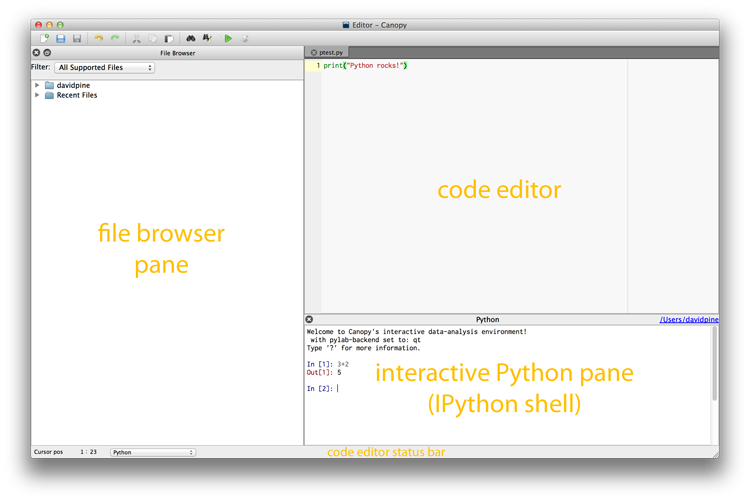
\includegraphics{CanopyWindow.png}}
\caption{Canopy window}\label{chap2/chap2_basics:fig-canopywindow}\end{figure}


\section{The Canopy window}
\label{chap2/chap2_basics:the-canopy-window}
\index{Canopy!window}
\index{Canopy!window}
The default Canopy window has three panes: the code editor, the interactive Python pane, and the file browser pane.  The \textbf{interactive Python pane} is the primary way that you interact with Python.  You can use it to run Python computer programs, test snippets of Python code, navigate your computer file directories, and perform system tasks like creating, moving, and deleting files and directories.  You will use the \textbf{code editor} to write and edit Python programs (or scripts), which are simply sequences of Python commands (code) stored in a file on your computer.  The \textbf{file browser pane} allows you to navigate your computer's file directory system in order to view and retrieve files on your computer.

The individual panes in the Canopy window are reconfigurable and detachable but we will leave them pretty much as they are for now.  However, you may want to adjust the overall size of the window to suit your computer screen.  You can find more information about Canopy in the \emph{Documentation Browser}, which you can access through the \emph{Welcome to Canopy} window.

\index{Canopy!IPython pane}

\section{The Interactive Python Pane}
\label{chap2/chap2_basics:the-interactive-python-pane}\label{chap2/chap2_basics:index-2}
The default input prompt of the interactive Python pane looks like this:

\begin{Verbatim}[commandchars=\\\{\}]
\PYG{g+go}{In [1]:}
\end{Verbatim}

\index{IPython!Canopy IPython pane}
This means that Canopy is running a particular version or ``shell'' of interactive Python called \textbf{IPython}. The IPython shell has been specifically designed for scientific and engineering use.  The standard Python interactive shell uses the prompt \code{\textgreater{}\textgreater{}\textgreater{}}.  You can pretty much do everything you want to do with either shell, but we will be using the IPython shell as we want to take advantage of some of its special features for scientific computing.

By typing short commands at the prompt, IPython can be used to perform various system tasks, such as running programs and creating and moving files around on your computer.  This is a different kind of computer interface than the icon-based interface (or ``graphical user interface'' GUI) that you usually use to communicate with your computer.  While it may seem more cumbersome for some tasks, it can be more powerful for other tasks, particularly those associated with programming.

Before getting started, we point out that like most modern computer languages, Python is \emph{case sensitive}.  That is, Python distinguishes between upper and lower case letters.  Thus, two words spelled the same but having different letters capitalized are treated as different names in Python.  Keep that in mind as we introduce different commands.


\subsection{Magic Functions}
\label{chap2/chap2_basics:magic-functions}
\index{IPython!magic functions}\index{magic functions!IPython}
IPython features a number of commands called ``magic'' commands that let you perform various useful tasks.  There are two types of magic commands, line magic commands that begin with \code{\%}---these are executed on a single line---and cell magic commands that begin with \code{\%\%}---these are executed on several lines.  Here we will concern ourselves only with line magic commands.

The first thing to know about magic commands is that you can toggle (turn on and off) the need to use the \code{\%} prefix for line magic commands by typing \code{\%automagic}.  By default, the \code{Automagic} switch is set to \code{ON} so you don't need the \code{\%} prefix.  To set \code{Automagic} to \code{OFF}, simply type \code{\%automagic} at the IPython prompt.  Cell magic commands always need the \code{\%\%} prefix.

In what follows below, we assume that the \code{Automagic} switch is set to \code{ON} so we omit the \code{\%} sign.

\index{IPython!navigation commands}

\subsubsection{Navigation Commands}
\label{chap2/chap2_basics:index-5}\label{chap2/chap2_basics:navigation-commands}
IPython recognizes several common navigation commands that are used under the Unix/Linux operating systems.  In the IPython shell, these few commands work on Macs, PCs, and Linux machines.

At the IPython prompt, type \code{cd \textasciitilde{}} (\emph{i.e.} ``\code{cd}'' -- ``space'' -- ``tilde'' , where tilde is found near the upper left part of most keyboards).  This will set your computer to its home (default) directory.  Next type \code{pwd} (\textbf{p}rint \textbf{w}orking \textbf{d}irectory) and press RETURN.  The console should return the name of the current directory of your computer.  It might look like this on a Mac:

\begin{Verbatim}[commandchars=\\\{\}]
\PYG{g+gp}{In [2]: }\PYG{n}{pwd}
\PYG{g+gr}{Out[2]: }\PYG{l+s}{u\PYGZsq{}}\PYG{l+s}{/Users/pine}\PYG{l+s}{\PYGZsq{}}
\end{Verbatim}

or this on a PC:

\begin{Verbatim}[commandchars=\\\{\}]
\PYG{g+gp}{In [3]: }\PYG{n}{pwd}
\PYG{g+gr}{Out[3]: }\PYG{n}{C}\PYG{p}{:}\PYGZbs{}\PYGZbs{}\PYG{n}{Users}\PYGZbs{}\PYGZbs{}\PYG{n}{pine}
\end{Verbatim}

The responses \code{Out{[}2{]}: u'/Users/pine'} for the Mac and \code{Out{[}3{]}: C:\textbackslash{}\textbackslash{}Users\textbackslash{}\textbackslash{}pine} for the PC mean the the current directory is \code{pine}, which is a subdirectory of \code{Users}.
Taken together \code{/Users/pine} on a Mac or \code{C:\textbackslash{}\textbackslash{}Users\textbackslash{}\textbackslash{}pine} on a PC is known as the \emph{path} of the current directory.
The path is just the name of a directory and the sequence of subdirectories in which it resides up to the \emph{root} directory.

Typing \code{cd ..} (``\code{cd}'' -- ``space'' -- two periods) moves the IPython shell up one directory in the directory tree, as illustrated by the set of commands below.

\begin{Verbatim}[commandchars=\\\{\}]
\PYG{g+gp}{In [4]: }\PYG{n}{cd} \PYG{o}{.}\PYG{o}{.}
\PYG{g+go}{/Users}

\PYG{g+gp}{In [5]: }\PYG{n}{pwd}
\PYG{g+gr}{Out[5]: }\PYG{l+s}{u\PYGZsq{}}\PYG{l+s}{/Users}\PYG{l+s}{\PYGZsq{}}
\end{Verbatim}

The directory moved up one from \code{/Users/pine} to \code{/Users}.  Now type \code{ls} (\textbf{l}i\textbf{s}t) and press \code{RETURN}.  The console should list the names of the files and subdirectories in the current directory.

\begin{Verbatim}[commandchars=\\\{\}]
\PYG{g+gp}{In [6]: }\PYG{n}{ls}
\PYG{g+go}{Shared/    pine/}
\end{Verbatim}

In this case, there are only two directories (indicated by the slash) and not files.  Type \code{cd \textasciitilde{}} again to return to your home directory and then type \code{pwd} to verify where you are in your directory tree.  {[}Technically, \code{ls} isn't a magic command, but typing it without the \code{\%} sign lists the contents of the current directory, irrespective of whether \code{Automagic} is \code{ON} or \code{OFF}.{]}

Let's create a directory within your documents directory that you can use to store your Python programs.  We will call it \code{PyProgs}.  First, return to your home directory by typing \code{cd \textasciitilde{}}.  To create directory \code{PyProgs}, type \code{mkdir PyProgs} (\textbf{m}a\textbf{k}e \textbf{dir}ectory).  Type \code{ls} to confirm that you have created \code{PyProgs} and then type \code{cd PyProgs} to switch to that directory.

Now let's say you want to return to the previous subdirectory, \code{Documents} or \code{My Documents}, which should be one up in the directory tree if you have followed along.  Type \code{cd ..} and then type \code{pwd}.  You should find that you are back in the previous directory, \code{Documents} or \code{My Documents}.  If you type \code{ls}, you should see the new directory \code{PyProgs} that you just created.


\subsubsection{More Magic Commands}
\label{chap2/chap2_basics:more-magic-commands}
\index{IPython!magic commands}
The most important magic command is \code{\%run} \emph{filename} where \emph{filename} is the name of a Python program you have created.  We haven't done this yet but include it here just for reference.  We will come back to this later.

Some other useful magic commands include \code{\%hist}, which lists the recent commands issued to the IPython terminal, and \code{\%edit}, which opens a new empty file in the code editor window.  Typing \code{\%edit} \emph{filename}, will open the file \emph{filename} if it exists in the current directory, or it will create a new file by that name if it does not, and will open it as a blank file in the code editor window.

There are a number of other magic commands.  You can get a list of them by typing \code{lsmagic}.

\begin{Verbatim}[commandchars=\\\{\}]
\PYG{g+gp}{In [7]: }\PYG{n}{lsmagic}
\PYG{g+go}{Available line magics:}
\PYG{g+go}{\PYGZpc{}alias  \PYGZpc{}alias\PYGZus{}magic  \PYGZpc{}autocall  \PYGZpc{}automagic  \PYGZpc{}bookmark  \PYGZpc{}cd}
\PYG{g+go}{\PYGZpc{}clear  \PYGZpc{}colors  \PYGZpc{}config  \PYGZpc{}connect\PYGZus{}info  \PYGZpc{}debug  \PYGZpc{}dhist  \PYGZpc{}dirs}
\PYG{g+go}{\PYGZpc{}doctest\PYGZus{}mode  \PYGZpc{}ed  \PYGZpc{}edit  \PYGZpc{}env  \PYGZpc{}gui  \PYGZpc{}guiref  \PYGZpc{}hist  \PYGZpc{}history}
\PYG{g+go}{\PYGZpc{}install\PYGZus{}default\PYGZus{}config  \PYGZpc{}install\PYGZus{}ext  \PYGZpc{}install\PYGZus{}profiles}
\PYG{g+go}{\PYGZpc{}killbgscripts  \PYGZpc{}less  \PYGZpc{}load  \PYGZpc{}load\PYGZus{}ext  \PYGZpc{}loadpy  \PYGZpc{}logoff  \PYGZpc{}logon}
\PYG{g+go}{\PYGZpc{}logstart \PYGZpc{}logstate  \PYGZpc{}logstop  \PYGZpc{}lsmagic  \PYGZpc{}macro  \PYGZpc{}magic  \PYGZpc{}man}
\PYG{g+go}{\PYGZpc{}more  \PYGZpc{}notebook  \PYGZpc{}page  \PYGZpc{}pastebin  \PYGZpc{}pdb  \PYGZpc{}pdef  \PYGZpc{}pdoc  \PYGZpc{}pfile}
\PYG{g+go}{\PYGZpc{}pinfo  \PYGZpc{}pinfo2  \PYGZpc{}popd  \PYGZpc{}pprint  \PYGZpc{}precision  \PYGZpc{}profile  \PYGZpc{}prun}
\PYG{g+go}{\PYGZpc{}psearch  \PYGZpc{}psource  \PYGZpc{}pushd  \PYGZpc{}pwd  \PYGZpc{}pycat  \PYGZpc{}pylab  \PYGZpc{}qtconsole}
\PYG{g+go}{\PYGZpc{}quickref  \PYGZpc{}recall  \PYGZpc{}rehashx  \PYGZpc{}reload\PYGZus{}ext  \PYGZpc{}rep  \PYGZpc{}rerun  \PYGZpc{}reset}
\PYG{g+go}{\PYGZpc{}reset\PYGZus{}selective  \PYGZpc{}run  \PYGZpc{}save  \PYGZpc{}sc  \PYGZpc{}store  \PYGZpc{}sx  \PYGZpc{}system  \PYGZpc{}tb}
\PYG{g+go}{\PYGZpc{}time  \PYGZpc{}timeit  \PYGZpc{}unalias  \PYGZpc{}unload\PYGZus{}ext  \PYGZpc{}who  \PYGZpc{}who\PYGZus{}ls  \PYGZpc{}whos}
\PYG{g+go}{\PYGZpc{}xdel  \PYGZpc{}xmode}

\PYG{g+go}{Available cell magics:}
\PYG{g+go}{\PYGZpc{}\PYGZpc{}!  \PYGZpc{}\PYGZpc{}bash  \PYGZpc{}\PYGZpc{}capture  \PYGZpc{}\PYGZpc{}file  \PYGZpc{}\PYGZpc{}javascript  \PYGZpc{}\PYGZpc{}latex  \PYGZpc{}\PYGZpc{}perl}
\PYG{g+go}{\PYGZpc{}\PYGZpc{}prun  \PYGZpc{}\PYGZpc{}pypy \PYGZpc{}\PYGZpc{}python  \PYGZpc{}\PYGZpc{}python3  \PYGZpc{}\PYGZpc{}ruby  \PYGZpc{}\PYGZpc{}script  \PYGZpc{}\PYGZpc{}sh  \PYGZpc{}\PYGZpc{}svg}
\PYG{g+go}{\PYGZpc{}\PYGZpc{}sx  \PYGZpc{}\PYGZpc{}system  \PYGZpc{}\PYGZpc{}timeit}

\PYG{g+go}{Automagic is ON, \PYGZpc{} prefix IS NOT needed for line magics.}
\end{Verbatim}

There are a lot of magic commands, most of which we don't need right now.  We will introduce them in the text as needed.


\subsection{System shell commands}
\label{chap2/chap2_basics:system-shell-commands}\label{chap2/chap2_basics:syscommands}
\index{IPython!system shell commands}
You can also run system shell commands from the IPython shell by typing \code{!} followed by a system shell command.  For Macs running OSX and for Linux machines, this means that Unix (or equivalently Linux) commands can be issued from the IPython prompt.  For PCs, this means that Windows (DOS) commands can be issued from the IPython prompt.  For example, typing  \code{!ls} (\textbf{l}i\textbf{s}t) and pressing RETURN lists all the files in the current directory on a Mac.  Typing \code{!dir} on a PC does essentially the same thing (note that system shell commands in Windows are \emph{not} case sensitive).

\index{IPython!tab completion}\index{tab completion!IPython}

\subsection{Tab completion}
\label{chap2/chap2_basics:tab-completion}\label{chap2/chap2_basics:index-8}
IPython also incorporates a number of shortcuts that make using the shell more efficient.  One of the most useful is \textbf{tab completion}.  Let's assume you have been following along and that your are in the directory  \code{Documents} or \code{My Documents}.  To switch to the directory \code{PyProgs}, you could type \code{cd PyProgs}.  Instead of doing that, type \code{cd PyP} and then press the \code{TAB} key.  This will complete the command, provided there is no ambiguity in how to finish the command.  In the present case, that would mean that there was no other subdirectory beginning with \code{PyP}.  Tab completion works with any command you type into the IPython terminal.  Try it out!  It will make your life more wonderful.

A related shortcut involves the \(\uparrow\) key.  If you type a command, say \code{cd} and then to press the \(\uparrow\) key, IPython will complete the \code{cd} command with the last instance of that command.  Thus, when you launch IPython, you can use this shortcut to take you to the directory you used when you last ran IPython.

You can also simply press the \(\uparrow\) key, which will simply recall the most recent command.  Repeated application of the \(\uparrow\) key scrolls though the most recent commands in reverse order.  The \(\downarrow\) key can be used to scroll in the other direction.


\subsection{Recap of commands}
\label{chap2/chap2_basics:recap-of-commands}
Let's recap the (magic) commands introduced above:
\begin{quote}
\begin{description}
\item[{\code{pwd}:}] \leavevmode
(\textbf{p}rint \textbf{w}orking \textbf{d}irectory) Prints the path of the current directory.

\item[{\code{ls}:}] \leavevmode
(\textbf{l}i\textbf{s}t)  Lists the names of the files and directories located in the current directory.

\item[{\code{mkdir} \emph{filename}:}] \leavevmode
(\textbf{m}a\textbf{k}e \textbf{dir}ectory)  Makes a new directory \emph{filename}.

\item[{\code{cd} \emph{directoryname}:}] \leavevmode
(\textbf{c}hange \textbf{d}irectory)  Changes the current directory to \emph{directoryname}.  Note: for this to work, \emph{directoryname} must be a subdirectory in the current directory.  Typing \code{cd \textasciitilde{}} changes to the home directory of your computer.  Typing \code{cd ..} moves the console one directory up in the directory tree.

\item[{\code{clear}:}] \leavevmode
Clears the IPython screen of previous commands.

\item[{\code{run} \emph{filename}:}] \leavevmode
Runs (executes) a Python script.  Described later in the section {\hyperref[chap2/chap2_basics:chap2-scriptexmp1]{\emph{Scripting Example 1}}}

\item[{Tab completion:}] \leavevmode
Provides convenient shortcuts, with or without the arrow keys, for executing commands in the IPython shell.

\end{description}
\end{quote}


\section{Interactive Python as a calculator}
\label{chap2/chap2_basics:interactive-python-as-a-calculator}
You can use the IPython shell to perform simple arithmatic calculations.  For example, to find the product \(3\times 15\), you type \code{3*15} at the \code{In} prompt and press \code{RETURN}:

\begin{Verbatim}[commandchars=\\\{\}]
\PYG{g+gp}{In [1]: }\PYG{l+m+mi}{3}\PYG{o}{*}\PYG{l+m+mi}{15}
\PYG{g+gr}{Out[1]: }\PYG{l+m+mi}{45}
\end{Verbatim}

Python returns the correct product, as expected.  You can do more complicated calculations:

\begin{Verbatim}[commandchars=\\\{\}]
\PYG{g+gp}{In [2]: }\PYG{l+m+mi}{6}\PYG{o}{+}\PYG{l+m+mi}{21}\PYG{o}{/}\PYG{l+m+mi}{3}
\PYG{g+gr}{Out[2]: }\PYG{l+m+mf}{13.0}
\end{Verbatim}

Let's try some more arithmetic:

\begin{Verbatim}[commandchars=\\\{\}]
\PYG{g+gp}{In [3]: }\PYG{p}{(}\PYG{l+m+mi}{6}\PYG{o}{+}\PYG{l+m+mi}{21}\PYG{p}{)}\PYG{o}{/}\PYG{l+m+mi}{3}
\PYG{g+gr}{Out[3]: }\PYG{l+m+mf}{9.0}
\end{Verbatim}

Notice that the effect of the parentheses in \code{In {[}3{]}: (6+21)/3} is to cause the addition to be performed first and then the division.  Without the parentheses, Python will always perform the multiplication and division operations \emph{before} performing the addition and subtraction operations.  The order in which arithmetic operations are performed is the same as for most calculators: exponentiation first, then multiplication or division, then addition or subtraction, then left to right.


\subsection{Binary arithmetic operations in Python}
\label{chap2/chap2_basics:binary-arithmetic-operations-in-python}
The table below lists the binary arithmatic operations in Python.  It has all the standard binary operators for arithmetic, plus a few you may not have seen before.
\begin{quote}

\begin{tabulary}{\linewidth}{|L|L|L|L|}
\hline
\textsf{\relax 
\textbf{Operation}
} & \textsf{\relax 
\textbf{Symbol}
} & \textsf{\relax 
\textbf{Example}
} & \textsf{\relax 
\textbf{Output}
}\\
\hline
addition
 & 
\code{+}
 & 
\code{12+7}
 & 
\code{19}
\\

subtraction
 & 
\code{-}
 & 
\code{12-7}
 & 
\code{5}
\\

multiplication
 & 
\code{*}
 & 
\code{12*7}
 & 
\code{84}
\\

division
 & 
\code{/}
 & 
\code{12/7}
 & 
\code{1.714285}
\\

floor division
 & 
\code{//}
 & 
\code{12//7}
 & 
\code{1}
\\

remainder
 & 
\code{\%}
 & 
\code{12\%7}
 & 
\code{5}
\\

exponentiation
 & 
\code{**}
 & 
\code{12**7}
 & 
\code{35831808}
\\
\hline\end{tabulary}

\end{quote}

\emph{Floor division}, designated by the symbols \code{//}, means divide and keep only the integer part without rounding.  \emph{Remainder}, designated by the symbols \code{\%}, gives the remainder of after a floor division.

\begin{notice}{warning}{Warning:}
Integer division is different in Python 2 and 3
\end{notice}

\index{integer division!Python 2 and 3 differences}
One peculiarity of all versions of Python prior to version 3 is that dividing two integers by each other yields the ``floor division'' result---another integer.  Therefore \code{12/7} yields \code{1} whereas \code{12./7} or \code{12/7.} or \code{12./7.} all yield \code{1.714285}.  Starting with version 3 of Python, all of the above expressions, including \code{3/2} yield \code{1.714285}.  Unfortunately, we are using version 2.7 of Python so \code{12/7} yields \code{1}.  You can force versions of Python prior to version 3 to divide integers like version 3 does by typing

\begin{Verbatim}[commandchars=\\\{\}]
\PYG{g+go}{from \PYGZus{}\PYGZus{}future\PYGZus{}\PYGZus{} import division}
\end{Verbatim}

at the beginning of an IPython session.  You only need to type it once and it works for the entire session.


\subsection{Types of numbers}
\label{chap2/chap2_basics:types-of-numbers}
There are four different types of numbers in Python: plain integers, long integers, floating point numbers, and complex numbers.

\textbf{Plain integers}, or simply \textbf{integers}, are 32 bits (binary digits) long, which means they extend from \(-2^{31}=-2147483648\) to \(2^{31}-1=2147483647\). One bit is used to store the sign of the integer so there are only 31 bits left---hence, the power of 31.  In Python, a number is automatically treated as an integer if is written without a decimal point and  it is within the bounds given above.  This means that \code{23}, written without a  decimal point, is an integer and \code{23.}, written with a decimal point, is a floating point number.  If an integer extends beyond the bounds of a simple integer, the it becomes a \textbf{long integer}, and is designated as such by an \code{L} following the last digit.  Here are some examples of integer arithmetic:

\begin{Verbatim}[commandchars=\\\{\}]
\PYG{g+gp}{In [4]: }\PYG{l+m+mi}{12}\PYG{o}{*}\PYG{l+m+mi}{3}
\PYG{g+gr}{Out[4]: }\PYG{l+m+mi}{36}

\PYG{g+gp}{In [5]: }\PYG{l+m+mi}{4}\PYG{o}{+}\PYG{l+m+mi}{5}\PYG{o}{*}\PYG{l+m+mi}{6}\PYG{o}{\PYGZhy{}}\PYG{p}{(}\PYG{l+m+mi}{21}\PYG{o}{*}\PYG{l+m+mi}{8}\PYG{p}{)}
\PYG{g+gr}{Out[5]: }\PYG{o}{\PYGZhy{}}\PYG{l+m+mi}{134}

\PYG{g+gp}{In [6]: }\PYG{l+m+mi}{11}\PYG{o}{/}\PYG{l+m+mi}{5}
\PYG{g+gr}{Out[6]: }\PYG{l+m+mf}{2.2}

\PYG{g+gp}{In [7]: }\PYG{l+m+mi}{11}\PYG{o}{/}\PYG{o}{/}\PYG{l+m+mi}{5}
\PYG{g+gr}{Out[7]: }\PYG{l+m+mi}{2}

\PYG{g+gp}{In [8]: }\PYG{l+m+mi}{9734828}\PYG{o}{*}\PYG{l+m+mi}{79372}    \PYG{c}{\PYGZsh{} product of these two large integers}
\PYG{g+gr}{Out[8]: }\PYG{l+m+mi+il}{772672768016L}    \PYG{c}{\PYGZsh{} is a long integer}
\end{Verbatim}

For the binary operators \code{+}, \code{-}, \code{*}, and \code{//}, the output is an integer if the inputs are integers.  The only exception is if the result of the calculation is out of the bounds of Python integers, in which case Python automatically converts the result to a long integer.  The output of the division operator \code{/} is a floating point as of version 3 of Python.  If an integer output is desired when two integers are divided, the floor division operator \code{//} must be used.

\textbf{Floating point} numbers are essentially rational numbers and can have a fractional part; integers, by their very nature, have no fractional part.  In most versions of Python running on PCs or Macs, floating point numbers go between approximately \(\pm 2 \times 10^{-308}\) and \(\pm 2 \times 10^{308}\).    Here are some examples of floating point arithmetic:

\begin{Verbatim}[commandchars=\\\{\}]
\PYG{g+gp}{In [9]: }\PYG{l+m+mf}{12.}\PYG{o}{*}\PYG{l+m+mf}{3.}
\PYG{g+gr}{Out[9]: }\PYG{l+m+mf}{36.0}

\PYG{g+gp}{In [10]: }\PYG{l+m+mf}{123.4}\PYG{o}{*}\PYG{p}{(}\PYG{o}{\PYGZhy{}}\PYG{l+m+mf}{53.9}\PYG{p}{)}\PYG{o}{/}\PYG{n}{sqrt}\PYG{p}{(}\PYG{l+m+mf}{5.}\PYG{p}{)}
\PYG{g+gr}{Out[10]: }\PYG{o}{\PYGZhy{}}\PYG{l+m+mf}{2974.5338992050501}

\PYG{g+gp}{In [11]: }\PYG{l+m+mf}{11.}\PYG{o}{/}\PYG{l+m+mf}{5.}
\PYG{g+gr}{Out[11]: }\PYG{l+m+mf}{2.2}

\PYG{g+gp}{In [12]: }\PYG{l+m+mf}{11.}\PYG{o}{/}\PYG{o}{/}\PYG{l+m+mf}{5.}
\PYG{g+gr}{Out[12]: }\PYG{l+m+mf}{2.0}

\PYG{g+gp}{In [13]: }\PYG{l+m+mf}{11.}\PYG{o}{\PYGZpc{}}\PYG{l+m+mf}{5.}
\PYG{g+gr}{Out[13]: }\PYG{l+m+mf}{1.0}

\PYG{g+gp}{In [14]: }\PYG{l+m+mf}{6.022e23}\PYG{o}{*}\PYG{l+m+mf}{300.}
\PYG{g+gr}{Out[14]: }\PYG{l+m+mf}{1.8066e+26}
\end{Verbatim}

Note that the result of any operation involving only floating point numbers as inputs is a real number, even in the cases where the floor division \code{//} or remainder \code{\%} operators are used.  The last output also illustrates an alternative way of writing floating point numbers as a mantissa followed by and \code{e} or \code{E} followed by a power of 10: so 1.23e-12 is equivalent to  \(1.23 \times 10^{-12}\).

We also sneaked into our calculations \code{sqrt}, the square root function.  We will have more to say about functions in a few pages.

\textbf{Complex numbers} are written in Python as a sum of a real and imaginary part.  For example, the complex number \(3-2i\) is represented as \code{3-2j} in Python where \code{j} represents \(\sqrt{-1}\).  Here are some examples of complex arithmetic:

\begin{Verbatim}[commandchars=\\\{\}]
\PYG{g+gp}{In [15]: }\PYG{p}{(}\PYG{l+m+mi}{2}\PYG{o}{+}\PYG{l+m+mi}{3j}\PYG{p}{)}\PYG{o}{*}\PYG{p}{(}\PYG{o}{\PYGZhy{}}\PYG{l+m+mi}{4}\PYG{o}{+}\PYG{l+m+mi}{9j}\PYG{p}{)}
\PYG{g+gr}{Out[15]: }\PYG{p}{(}\PYG{o}{\PYGZhy{}}\PYG{l+m+mi}{35}\PYG{o}{+}\PYG{l+m+mi}{6j}\PYG{p}{)}

\PYG{g+gp}{In [16]: }\PYG{p}{(}\PYG{l+m+mi}{2}\PYG{o}{+}\PYG{l+m+mi}{3j}\PYG{p}{)}\PYG{o}{/}\PYG{p}{(}\PYG{o}{\PYGZhy{}}\PYG{l+m+mi}{4}\PYG{o}{+}\PYG{l+m+mi}{9j}\PYG{p}{)}
\PYG{g+gr}{Out[16]: }\PYG{p}{(}\PYG{l+m+mf}{0.1958762886597938}\PYG{o}{\PYGZhy{}}\PYG{l+m+mf}{0.3092783505154639j}\PYG{p}{)}

\PYG{g+gp}{In [17]: }\PYG{n}{sqrt}\PYG{p}{(}\PYG{o}{\PYGZhy{}}\PYG{l+m+mi}{3}\PYG{p}{)}
\PYG{g+gr}{Out[17]: }\PYG{n}{nan}

\PYG{g+gp}{In [18]: }\PYG{n}{sqrt}\PYG{p}{(}\PYG{o}{\PYGZhy{}}\PYG{l+m+mi}{3}\PYG{o}{+}\PYG{l+m+mi}{0j}\PYG{p}{)}
\PYG{g+gr}{Out[18]: }\PYG{l+m+mf}{1.7320508075688772j}
\end{Verbatim}

Notice that to obtain the expected result or \(\sqrt{-3}\), you must write the argument of the square root function as a complex number.  Otherwise, Python returns \code{nan} (not a number).

If you multiply an integer by a floating point number, the result is a floating point number.  Similarly, if you multiply a floating point number by a complex number, the result is a complex number.  Python always promotes the result to the most complex of the inputs.

\index{Python!module}\index{module!NumPy}\index{NumPy!module}\index{module!SciPy}\index{SciPy!module}\index{module!MatPlotLib}\index{MatPlotLib!module}

\section{Python Modules}
\label{chap2/chap2_basics:python-modules}\label{chap2/chap2_basics:index-10}
The Python computer language consists of a ``core'' language plus a vast collection of supplementary software that is contained in \textbf{modules}.  Many of these modules come with the standard Python distribution and provide added functionality for performing computer system tasks.  Other modules provide more specialized capabilities that not every user may want.  You can think of these modules as a kind of library from which you can borrow according to your needs.

We will need three Python modules that are not part of the core Python distribution, but are nevertheless widely used for scientific computing.  The three modules are
\begin{quote}
\begin{description}
\item[{NumPy}] \leavevmode
is the standard Python package for scientific computing with Python.  It provides the all-important \code{array} data structure, which is at the very heart of NumPy.  In also provides tools for creating and manipulating arrays, including indexing and sorting, as well as basic logical operations and element-by-element arithmetic operations like addition, subtraction, multiplication, division, and exponentiation.  It includes the basic mathematical functions of trigonometry, exponentials, and logarithms, as well vast collection of special functions (Bessel functions, \emph{etc.}), statistical functions, and random number generators.  It also includes a large number of linear algebra routines that overlap with those in SciPy, although the SciPy routines tend to be more complete.  You can find more information about NumPy at \href{http://docs.scipy.org/doc/numpy/reference/index.html}{http://docs.scipy.org/doc/numpy/reference/index.html}.

\item[{SciPy}] \leavevmode
provides a wide spectrum of mathematical functions and numerical routines for Python.  SciPy makes extensive use of NumPy arrays so when you import SciPy, you should always import NumPy too.  In addition to providing basic mathematical functions, SciPy provides Python ``wrappers'' for numerical software written in other languages, like Fortran, C, or C++.  A  ``wrapper'' provides a transparent easy-to-use Python interface to standard numerical software, such as routines for doing curve fitting and numerically solving differential equations.  SciPy greatly extends the power of Python and saves you the trouble of writing software in Python that someone else has already written and optimized in some other language.  You can find more information about SciPy at \href{http://docs.scipy.org/doc/scipy/reference/}{http://docs.scipy.org/doc/scipy/reference/}.

\item[{MatPlotLib}] \leavevmode
is the standard Python package for making two and three dimensional plots.  MatPlotLib makes extensive use of NumPy arrays.  You will make all of your plots in Python using this package.  You can find more information about MatPlotLib at \href{http://MatPlotLib.sourceforge.net/}{http://MatPlotLib.sourceforge.net/}.

\end{description}
\end{quote}

We will use these three modules extensively and therefore will provide introductions to their capabilities as we develop Python in this manual.  The links above provide much more extensive information and you will certainly want to refer to them from time to time.

These modules, NumPy, MatPlotLib, and SciPy, are built into the IPython shell so we can use them freely in that environment.  Later, when we introduce Python programs (or scripts), we will see that in those cases you must explicitly load these modules using the \code{import} command to have access to them.

Finally, we note that you can write your own Python modules.  They are a convenient way of packaging and storing Python code so that you can reuse it.  We defer learning about how to write modules until after we have learned about Python.


\section{Python functions: a first look}
\label{chap2/chap2_basics:python-functions-a-first-look}\label{chap2/chap2_basics:chap2-numpyfuncs}
A function in Python is similar to a mathematical function.  In consists of a name and one or more arguments contained inside parentheses, and it produces some output.  For example, the NumPy function \code{sin(x)} calculates the sine of the number \code{x} (where \code{x} is expressed in radians).  Let's try it out in the IPython shell:

\begin{Verbatim}[commandchars=\\\{\}]
\PYG{g+gp}{In [1]: }\PYG{n}{sin}\PYG{p}{(}\PYG{l+m+mf}{0.5}\PYG{p}{)}
\PYG{g+gr}{Out[1]: }\PYG{l+m+mf}{0.47942553860420301}
\end{Verbatim}

The argument of the function can be a number or any kind of expression whose output produces a number.  For example, the function \code{log(x)} calculates the natural logarithm of \code{x}.  All of the following expressions are legal and produce the expected output:

\begin{Verbatim}[commandchars=\\\{\}]
\PYG{g+gp}{In [2]: }\PYG{n}{log}\PYG{p}{(}\PYG{n}{sin}\PYG{p}{(}\PYG{l+m+mf}{0.5}\PYG{p}{)}\PYG{p}{)}
\PYG{g+gr}{Out[2]: }\PYG{o}{\PYGZhy{}}\PYG{l+m+mf}{0.73516668638531424}

\PYG{g+gp}{In [3]: }\PYG{n}{log}\PYG{p}{(}\PYG{n}{sin}\PYG{p}{(}\PYG{l+m+mf}{0.5}\PYG{p}{)}\PYG{o}{+}\PYG{l+m+mf}{1.0}\PYG{p}{)}
\PYG{g+gr}{Out[3]: }\PYG{l+m+mf}{0.39165386283471759}

\PYG{g+gp}{In [4]: }\PYG{n}{log}\PYG{p}{(}\PYG{l+m+mf}{5.5}\PYG{o}{/}\PYG{l+m+mf}{1.2}\PYG{p}{)}
\PYG{g+gr}{Out[4]: }\PYG{l+m+mf}{1.5224265354444708}
\end{Verbatim}

\index{NumPy!functions}\index{functions!NumPy}

\subsection{Some NumPy functions}
\label{chap2/chap2_basics:some-numpy-functions}\label{chap2/chap2_basics:index-11}
\index{NumPy!functions}\index{functions!NumPy}
NumPy includes an extensive library of mathematical functions.  In the table below, we list some of the most useful ones.  A much more complete list is available at \href{http://docs.scipy.org/doc/numpy/reference/ufuncs.html\#math-operations}{http://docs.scipy.org/doc/numpy/reference/ufuncs.html\#math-operations}.
\begin{quote}

\begin{tabulary}{\linewidth}{|L|L|}
\hline
\textsf{\relax 
\textbf{Function}
} & \textsf{\relax 
\textbf{Description}
}\\
\hline
\code{sqrt(x)}
 & 
Square root of \(x\)
\\

\code{exp(x)}
 & 
Exponential of x, \emph{i.e.} \(e^{x}\)
\\

\code{log(x)}
 & 
Natural log of x, \emph{i.e.} \(\ln x\)
\\

\code{log10(x)}
 & 
Base 10 log of \(x\)
\\

\code{degrees(x)}
 & 
Converts \(x\) from radians to degrees
\\

\code{radians(x)}
 & 
Converts \(x\) from degrees to radians
\\

\code{sin(x)}
 & 
Sine of \(x\) (\(x\) in radians)
\\

\code{cos(x)}
 & 
Cosine \(x\) (\(x\) in radians)
\\

\code{tan(x)}
 & 
Tangent \(x\) (\(x\) in radians)
\\

\code{arcsin(x)}
 & 
Arc sine (in radians) of \(x\)
\\

\code{arccos(x)}
 & 
Arc cosine (in radians) of \(x\)
\\

\code{arctan(x)}
 & 
Arc tangent (in radians) of \(x\)
\\

\code{fabs(x)}
 & 
Absolute value of \(x\)
\\

\code{round(x)}
 & 
Rounds a float to nearest integer
\\

\code{floor(x)}
 & 
Rounds a float \emph{down} to nearest integer
\\

\code{ceil(x)}
 & 
Rounds a float \emph{up} to nearest integer
\\

\code{sign(x)}
 & 
-1 if \(x<0\), +1 if \(x>0\), 0 if \(x=0\)
\\
\hline\end{tabulary}

\end{quote}

The functions discussed here all have one input and one output.  Python functions can, in general, have multiple inputs and multiple outputs.  We will discuss these and other features of functions later when we take up functions in the context of user-defined functions.


\subsection{Keyword arguments}
\label{chap2/chap2_basics:keyword-arguments}
In addition to regular arguments, Python functions can have keyword arguments (\code{kwargs}).  Keyword arguments are \emph{optional} arguments that need not be specified when a function is called.  See {\hyperref[chap5/chap5_plot:chap5basicplotting]{\emph{Basic plotting}}} for examples of the use of keyword arguments.  For the moment, we don't need them so we defer a full discussion of keyword arguments until we introduce them in the section on {\hyperref[chap7/chap7_funcs:userdefdfuncs]{\emph{User-defined functions}}}.


\section{Variables}
\label{chap2/chap2_basics:variables}

\subsection{Names and the assignment operator}
\label{chap2/chap2_basics:names-and-the-assignment-operator}
\index{variable}\index{assignment operator}
A variable is a name that is used to store data.  It can be used to store different kinds of data, but here we consider the simplest case where the data is a single numerical value.  Here are a few examples:

\begin{Verbatim}[commandchars=\\\{\}]
\PYG{g+gp}{In [1]: }\PYG{n}{a} \PYG{o}{=} \PYG{l+m+mi}{23}

\PYG{g+gp}{In [2]: }\PYG{n}{p}\PYG{p}{,} \PYG{n}{q} \PYG{o}{=} \PYG{l+m+mf}{83.4}\PYG{p}{,} \PYG{n}{sqrt}\PYG{p}{(}\PYG{l+m+mi}{2}\PYG{p}{)}
\end{Verbatim}

The equal sign ``\code{=}'' is the \emph{assignment operator}.  In the first statement, it assigns the value of 23 to the variable \code{a}.  In the second statement it assigns a value of 83.4 to \code{p} and a value of 1.4142135623730951 to \code{q}.  To be more precise, the name of a variable, such as \code{a}, is associated with a \emph{memory location} in your computer; the assignment variable tells the computer to put a particular piece of data, in this case a numerical value, in that memory location.  Note that Python stores the \emph{numerical value}, not the expression used to generate it.  Thus, \code{q} is assigned the 17-digit number 1.4142135623730951 generated by evaluating the expression \code{sqrt(2)}, \emph{not} with \(\sqrt{2}\).  (Actually the value of \code{q} is stored as a  binary, base 2, number using scientific notation with a mantissa and an exponent.)

Suppose we write

\begin{Verbatim}[commandchars=\\\{\}]
\PYG{g+gp}{In [3]: }\PYG{n}{b} \PYG{o}{=} \PYG{n}{a}
\end{Verbatim}

In this case Python associates a new memory location with the name \code{b}, distinct from the one associated with \code{a}, and sets the value stored at that memory location to 23, the value of \code{a}.  The following sequence of statements demonstrate that fact.  Can you see how?  Notice that simply typing a variable name and pressing \code{Return} prints out the value of the variable.

\begin{Verbatim}[commandchars=\\\{\}]
\PYG{g+gp}{In [4]: }\PYG{n}{a}\PYG{o}{=}\PYG{l+m+mi}{23}

\PYG{g+gp}{In [5]: }\PYG{n}{b}\PYG{o}{=}\PYG{n}{a}

\PYG{g+gp}{In [6]: }\PYG{n}{a}
\PYG{g+gr}{Out[6]: }\PYG{l+m+mi}{23}

\PYG{g+gp}{In [7]: }\PYG{n}{b}
\PYG{g+gr}{Out[7]: }\PYG{l+m+mi}{23}

\PYG{g+gp}{In [8]: }\PYG{n}{a}\PYG{o}{=}\PYG{l+m+mi}{12}

\PYG{g+gp}{In [9]: }\PYG{n}{a}
\PYG{g+gr}{Out[9]: }\PYG{l+m+mi}{12}

\PYG{g+gp}{In [10]: }\PYG{n}{b}
\PYG{g+gr}{Out[10]: }\PYG{l+m+mi}{23}
\end{Verbatim}

The assignment variable works from right to left; that is, it assigns the value of the number on the right to the variable name on the left.  Therefore, the statement ``\code{5=a}'' makes no sense in Python.  The assignment operator ``\code{=}'' in Python is not equivalent to the equals sign ``\(=\)'' we are accustomed to in algebra.

The assignment operator can be used to increment or change the value of a variable

\begin{Verbatim}[commandchars=\\\{\}]
\PYG{g+gp}{In [11]: }\PYG{n}{b} \PYG{o}{=} \PYG{n}{b}\PYG{o}{+}\PYG{l+m+mi}{1}

\PYG{g+gp}{In [12]: }\PYG{n}{b}
\PYG{g+gr}{Out[12]: }\PYG{l+m+mi}{24}
\end{Verbatim}

The statement, \code{b = b+1} makes no sense in algebra, but in Python (and most computer languages), it makes perfect sense: it means ``add 1 to the current value of \code{b} and assign the result to \code{b}.''  This  construction appears so often in computer programming that there is a special set of operators to perform such changes to a variable: \code{+=}, \code{-=}, \code{*=}, and \code{/=}.  Here are some examples of how they work:

\begin{Verbatim}[commandchars=\\\{\}]
\PYG{g+gp}{In [13]: }\PYG{n}{c} \PYG{p}{,} \PYG{n}{d} \PYG{o}{=} \PYG{l+m+mi}{4}\PYG{p}{,} \PYG{l+m+mf}{7.92}

\PYG{g+gp}{In [14]: }\PYG{n}{c} \PYG{o}{+}\PYG{o}{=} \PYG{l+m+mi}{2}

\PYG{g+gp}{In [15]: }\PYG{n}{c}
\PYG{g+gr}{Out[15]: }\PYG{l+m+mi}{6}

\PYG{g+gp}{In [16]: }\PYG{n}{c} \PYG{o}{*}\PYG{o}{=} \PYG{l+m+mi}{3}

\PYG{g+gp}{In [16]: }\PYG{n}{c}
\PYG{g+gr}{Out[16]: }\PYG{l+m+mi}{18}

\PYG{g+gp}{In [17]: }\PYG{n}{d} \PYG{o}{/}\PYG{o}{=} \PYG{o}{\PYGZhy{}}\PYG{l+m+mi}{2}

\PYG{g+gp}{In [17]: }\PYG{n}{d}
\PYG{g+gr}{Out[17]: }\PYG{o}{\PYGZhy{}}\PYG{l+m+mf}{3.96}

\PYG{g+gp}{In [18]: }\PYG{n}{d} \PYG{o}{\PYGZhy{}}\PYG{o}{=} \PYG{l+m+mi}{4}

\PYG{g+gp}{In [19]: }\PYG{n}{d}
\PYG{g+gr}{Out[19]: }\PYG{o}{\PYGZhy{}}\PYG{l+m+mf}{7.96}
\end{Verbatim}

Verify that you understand how the above operations work.

\index{variable names}

\subsection{Legal and recommended variable names}
\label{chap2/chap2_basics:index-14}\label{chap2/chap2_basics:legal-and-recommended-variable-names}
Variable names in Python must start with a letter, and can be followed by as many alphanumeric characters as you like. Spaces are not allowed in variable names.  However, the underscore character ``\code{\_}'' is allowed, but no other character that is not a letter or a number is permitted.

Recall that Python is \emph{case sensitive}, so the variable \code{a} is distinct from the variable \code{A}.

We recommend giving your variables descriptive names as in the following calculation:

\begin{Verbatim}[commandchars=\\\{\}]
\PYG{g+gp}{In [20]: }\PYG{n}{distance} \PYG{o}{=} \PYG{l+m+mf}{34.}

\PYG{g+gp}{In [21]: }\PYG{n}{time\PYGZus{}traveled} \PYG{o}{=} \PYG{l+m+mf}{0.59}

\PYG{g+gp}{In [22]: }\PYG{n}{velocity} \PYG{o}{=} \PYG{n}{distance}\PYG{o}{/}\PYG{n}{time\PYGZus{}traveled}

\PYG{g+gp}{In [23]: }\PYG{n}{velocity}
\PYG{g+gr}{Out[23]: }\PYG{l+m+mf}{57.6271186440678}
\end{Verbatim}

The variable names \code{distance}, \code{time\_traveled}, and \code{velocity} immediately remind you of what is being calculated here.  This is good practice.  But so is keeping variable names reasonably short, so don't go nuts!

\index{reserved words}

\subsection{Reserved words in Python}
\label{chap2/chap2_basics:index-15}\label{chap2/chap2_basics:reserved-words-in-python}
There are also some names or words that are reserved by Python for special purposes or functions.  You must avoid using these names, which are provided here for your reference:
\begin{quote}

\begin{tabulary}{\linewidth}{|L|L|L|L|L|}
\hline

\code{and}
 & 
\code{del}
 & 
\code{from}
 & 
\code{not}
 & 
\code{while}
\\

\code{as}
 & 
\code{elif}
 & 
\code{global}
 & 
\code{or}
 & 
\code{with}
\\

\code{assert}
 & 
\code{else}
 & 
\code{if}
 & 
\code{pass}
 & 
\code{yield}
\\

\code{break}
 & 
\code{except}
 & 
\code{import}
 & 
\code{print}
 & \\

\code{class}
 & 
\code{exec}
 & 
\code{in}
 & 
\code{raise}
 & \\

\code{continue}
 & 
\code{finally}
 & 
\code{is}
 & 
\code{return}
 & \\

\code{def}
 & 
\code{for}
 & 
\code{lambda}
 & 
\code{try}
 & \\
\hline\end{tabulary}

\end{quote}

In addition, you should not use function names, like \code{sin}, \code{cos}, and \code{sqrt}, defined in the SciPy, NumPy, or any other library that you are using.

\index{scripts}\index{programs}

\section{Script files and programs}
\label{chap2/chap2_basics:index-16}\label{chap2/chap2_basics:script-files-and-programs}
Performing calculations in the IPython shell is handy if the calculations are short.  But calculations quickly become tedious when they are more than a few lines long.  If you discover you made a mistake at some early step, for example, you may have to go back and retype all the steps subsequent to the error.  The solution to this problem is to save your code in a file.  Saving code in a file means you can just correct the error and rerun the code without having to retype it.  Saving code can also be useful if you want to reuse it later, perhaps with different inputs.

When we save code in a computer file, we call the sequence of commands stored in the file a \emph{script} or a \emph{program} or sometimes a \emph{routine}.  Programs can become quite sophisticated and complex.  Here we are only going to introduce the simplest features of programming by writing a very simple script.  Much later, we will introduce some of the more advanced features of programming.

\index{Canopy!Code Editor}\index{Canopy!tab completion}\index{tab completion!Canopy}
To write a script you need a text editor.  In principle, any text editor will do, but it's more convenient to use an editor that was designed for the task.  We are going to use the \textbf{Code Editor} in the Canopy window that appears when you launch the Canopy application (see  {\hyperref[chap2/chap2_basics:fig-canopywindow]{\emph{Canopy window}}}).  This editor, like most good programming editors, provides syntax highlighting, which color codes key words, comments, and other features of the Python syntax according to their function, and thus makes it easier to read the code and easier to spot programming mistakes.  The Canopy code editor also provides syntax checking, much like a spell-checker in a word processing program, that identifies many coding errors.  This can greatly speed the coding process.  Tab completion also works in the Canopy Code Editor.


\subsection{Scripting Example 1}
\label{chap2/chap2_basics:chap2-scriptexmp1}\label{chap2/chap2_basics:scripting-example-1}
Let's work through an example to see how scripting works.  Suppose you are going on a road trip and you would like to estimate how long the drive will take, how much gas you will need, and the cost of the gas.  It's a simple calculation.  As inputs, you will need the distance of the trip, your average speed, the cost of gasoline, and the mileage of your car.

Writing a script to do these calculations is straightforward.  First, launch Canopy and open the code editor.  You should see a tab with the word \code{untitled} at the top left of the code editor pane (see {\hyperref[chap2/chap2_basics:fig-canopywindow]{\emph{Canopy window}}}).  If you don't, go to the \code{File} menu and select \code{New File}.  Use the mouse to place your cursor at the top of the code editor pane.  Enter the following code and \emph{save the code} in a file called \code{myTrip.py} in the \code{PyProgs} folder you created earlier.  This stores your script (or program) on your computer's disk.  The exact name of the file is not important but the extension \code{.py} is essential.  It tells the computer, and more importantly Python, that this is a Python program.

\begin{Verbatim}[commandchars=\\\{\}]
\PYG{c}{\PYGZsh{} Calculates time, gallons of gas used, and cost of gasoline for}
\PYG{c}{\PYGZsh{} a trip}
\PYG{n}{distance} \PYG{o}{=} \PYG{l+m+mf}{400.}         \PYG{c}{\PYGZsh{} miles}
\PYG{n}{mpg} \PYG{o}{=} \PYG{l+m+mf}{30.}               \PYG{c}{\PYGZsh{} car mileage}
\PYG{n}{speed} \PYG{o}{=} \PYG{l+m+mf}{60.}             \PYG{c}{\PYGZsh{} average speed}
\PYG{n}{costPerGallon} \PYG{o}{=} \PYG{l+m+mf}{4.10}    \PYG{c}{\PYGZsh{} price of gas}

\PYG{n}{time} \PYG{o}{=} \PYG{n}{distance}\PYG{o}{/}\PYG{n}{speed}
\PYG{n}{gallons} \PYG{o}{=} \PYG{n}{distance}\PYG{o}{/}\PYG{n}{mpg}
\PYG{n}{cost} \PYG{o}{=} \PYG{n}{gallons}\PYG{o}{*}\PYG{n}{costPerGallon}
\end{Verbatim}

The number (or hash) symbol \code{\#} is the ``comment'' character in Python; anything on a line following \code{\#} is ignored when the code is executed.  Judicious use of comments in your code will make your code much easier to understand days, weeks, or months after the time you wrote it.  Use comments generously.

Python ignores blank spaces or ``white space'' as it is sometimes called. The statement \code{costPerGallon = 4.10} in the above program could equally well be written as \code{costPerGallon=4.10} without the spaces before and after the \code{=} assignment operator; either way the statement means the same thing.  Similarly, the white space after \code{costPerGallon = 4.10} but before the comment (hash) symbol is also ignored by Python.  The idea is that you should use white space to make your program more readable.

Now you are ready to run the code.  Before doing so, you first need to use the IPython console to move to the \code{PyProgs} directory where the file containing the code resides.  From the IPython console, use the \code{cd} command to move to the \code{PyProgs} directory.  For example, you might type

\begin{Verbatim}[commandchars=\\\{\}]
\PYG{g+gp}{In [1]: }\PYG{n}{cd} \PYG{o}{\PYGZti{}}\PYG{o}{/}\PYG{n}{Documents}\PYG{o}{/}\PYG{n}{PyProgs}\PYG{o}{/}
\end{Verbatim}

To  \emph{run} or \emph{execute} a script, simply type \code{run} \emph{filename}, which in this case means type \code{run myTrip.py}.  When you run a script, Python simply executes the sequence of commands in the order they appear.

\begin{Verbatim}[commandchars=\\\{\}]
\PYG{g+gp}{In [2]: }\PYG{n}{run} \PYG{n}{myTrip}\PYG{o}{.}\PYG{n}{py}
\end{Verbatim}

Once you have run the script, you can see the values of the variables calculated in the script simply by typing the name of the variable.  IPython responds with the value of that variable.

\begin{Verbatim}[commandchars=\\\{\}]
\PYG{g+gp}{In [3]: }\PYG{n}{time}
\PYG{g+gr}{Out[3]: }\PYG{l+m+mf}{6.666666666666667}

\PYG{g+gp}{In [4]: }\PYG{n}{gallons}
\PYG{g+gr}{Out[4]: }\PYG{l+m+mf}{13.333333333333334}

\PYG{g+gp}{In [5]: }\PYG{n}{cost}
\PYG{g+gr}{Out[5]: }\PYG{l+m+mf}{54.666666666666664}
\end{Verbatim}

You can change the number of digits IPython displays using the command \code{\%precision}:

\begin{Verbatim}[commandchars=\\\{\}]
\PYG{g+gp}{In [6]: }\PYG{o}{\PYGZpc{}}\PYG{n}{precision} \PYG{l+m+mi}{2}
\PYG{g+gr}{Out[6]: }\PYG{l+s}{u\PYGZsq{}}\PYG{l+s+si}{\PYGZpc{}.2f}\PYG{l+s}{\PYGZsq{}}

\PYG{g+gp}{In [7]: }\PYG{n}{time}
\PYG{g+gr}{Out[7]: }\PYG{l+m+mf}{6.67}

\PYG{g+gp}{In [8]: }\PYG{n}{gallons}
\PYG{g+gr}{Out[8]: }\PYG{l+m+mf}{13.33}

\PYG{g+gp}{In [9]: }\PYG{n}{cost}
\PYG{g+gr}{Out[9]: }\PYG{l+m+mf}{54.67}
\end{Verbatim}

Typing \code{\%precision} returns IPython to its default state;  \code{\%precision \%e} causes IPython to display numbers in exponential format (scientific notation).


\subsubsection{Note about printing}
\label{chap2/chap2_basics:printnote}\label{chap2/chap2_basics:note-about-printing}
If you want your script to return the value of a variable (that is, print the value of the variable to your computer screen), use the \code{print} function.  For example, at the end of our script, if we include the code

\begin{Verbatim}[commandchars=\\\{\}]
\PYG{k}{print}\PYG{p}{(}\PYG{n}{time}\PYG{p}{)}
\PYG{k}{print}\PYG{p}{(}\PYG{n}{gallons}\PYG{p}{)}
\PYG{k}{print}\PYG{p}{(}\PYG{n}{cost}\PYG{p}{)}
\end{Verbatim}

the script will return the values of the variables \code{time}, \code{gallons}, and \code{cost} that the script calculated.  We will discuss the \code{print} function in much greater detail, as well as other methods for data output, in Chapter 4 on {\hyperref[chap4/chap4_io:chap4]{\emph{Input and Output}}}.


\subsection{Scripting Example 2}
\label{chap2/chap2_basics:scripting-example-2}\label{chap2/chap2_basics:chap2-scriptexmp2}
Let's try another problem.  Suppose you want to find the distance between two Cartesian coordinates \((x_1, y_1, z_1)\) and \((x_2, y_2, z_2)\).  The distance is given by the formula
\begin{gather}
\begin{split}\Delta r = \sqrt{(x_2-x_1)^2+(y_2-y_1)^2+(z_2-z_1)^2}\end{split}\notag
\end{gather}
Now let's write a script to do this calculation and save it in a file called \code{twoPointDistance.py}.

\begin{Verbatim}[commandchars=\\\{\},numbers=left,firstnumber=1,stepnumber=1]
\PYG{c}{\PYGZsh{} Calculates the distance between two 3d Cartesian coordinates}
\PYG{k+kn}{import} \PYG{n+nn}{numpy} \PYG{k+kn}{as} \PYG{n+nn}{np}

\PYG{n}{x1}\PYG{p}{,} \PYG{n}{y1}\PYG{p}{,} \PYG{n}{z1} \PYG{o}{=} \PYG{l+m+mf}{23.7}\PYG{p}{,} \PYG{o}{\PYGZhy{}}\PYG{l+m+mf}{9.2}\PYG{p}{,} \PYG{o}{\PYGZhy{}}\PYG{l+m+mf}{7.8}
\PYG{n}{x2}\PYG{p}{,} \PYG{n}{y2}\PYG{p}{,} \PYG{n}{z2} \PYG{o}{=} \PYG{o}{\PYGZhy{}}\PYG{l+m+mf}{3.5}\PYG{p}{,} \PYG{l+m+mf}{4.8}\PYG{p}{,} \PYG{l+m+mf}{8.1}

\PYG{n}{dr} \PYG{o}{=} \PYG{n}{np}\PYG{o}{.}\PYG{n}{sqrt}\PYG{p}{(} \PYG{p}{(}\PYG{n}{x2}\PYG{o}{\PYGZhy{}}\PYG{n}{x1}\PYG{p}{)}\PYG{o}{*}\PYG{o}{*}\PYG{l+m+mi}{2} \PYG{o}{+} \PYG{p}{(}\PYG{n}{y2}\PYG{o}{\PYGZhy{}}\PYG{n}{y1}\PYG{p}{)}\PYG{o}{*}\PYG{o}{*}\PYG{l+m+mi}{2} \PYG{o}{+} \PYG{p}{(}\PYG{n}{z2}\PYG{o}{\PYGZhy{}}\PYG{n}{z1}\PYG{p}{)}\PYG{o}{*}\PYG{o}{*}\PYG{l+m+mi}{2} \PYG{p}{)}
\end{Verbatim}

We have introduced extra spaces into some of the expressions to improve readability.  They are not necessary; where and whether you include them is largely a matter of taste.

There are two important differences between the code above and the commands we would have written into the IPython console to execute the same set of commands.  The first is the statement on the second line

\begin{Verbatim}[commandchars=\\\{\}]
\PYG{o}{.}\PYG{o}{.}\PYG{o}{.}
\PYG{k+kn}{import} \PYG{n+nn}{numpy} \PYG{k+kn}{as} \PYG{n+nn}{np}
\PYG{o}{.}\PYG{o}{.}\PYG{o}{.}
\end{Verbatim}

and the second is the ``\code{np.}'' in front of the \code{sqrt} function on the last line.  If you leave out the \code{import numpy as np} line and remove the \code{np.} in front of the \code{sqrt} function, you will get the following error message

\begin{Verbatim}[commandchars=\\\{\}]
\PYG{g+go}{\PYGZhy{}\PYGZhy{}\PYGZhy{}\PYGZhy{}\PYGZgt{} 7 dr = sqrt( (x2\PYGZhy{}x1)**2 + (y2\PYGZhy{}y1)**2 + (z2\PYGZhy{}z1)**2 )}

\PYG{g+go}{NameError: name \PYGZsq{}sqrt\PYGZsq{} is not defined}
\end{Verbatim}

The reason for the error is that the \code{sqrt} function is not a part of core Python.  But it is a part of the NumPy module discussed earlier.  To make the NumPy library available to the script, you need to add the statement \code{import numpy as np}.  Then, when you call a NumPy function, you need to write the function with the \code{np.} prefix.  Failure to do either will result in a error message.  Now we can run the script.

\begin{Verbatim}[commandchars=\\\{\}]
\PYG{g+gp}{In [10]: }\PYG{n}{run} \PYG{n}{twoPointDistance}\PYG{o}{.}\PYG{n}{py}

\PYG{g+gp}{In [11]: }\PYG{n}{dr}
\PYG{g+gr}{Out[11]: }\PYG{l+m+mf}{34.48}
\end{Verbatim}

The script works as expected.

The reason we do not have to import NumPy when working in the IPython shell is that it is done automatically when the IPython shell is launched.  Similarly, the package MatPlotLib is also automatically loaded (imported) when IPython is launched.  However, when a script or program is executed, it is run on its own outside the IPython shell, even if the command to run the script is executed from the IPython shell.

\index{line continuation}

\subsubsection{Line continuation}
\label{chap2/chap2_basics:index-18}\label{chap2/chap2_basics:line-continuation}
From time to time, a line of code in a script will be unusually long, which can make the code difficult to read.  In such cases, it is advisable to split the code onto several lines. For example, line 7 in the preceding script could be written as

\begin{Verbatim}[commandchars=\\\{\}]
\PYG{g+go}{dr = np.sqrt( (x2\PYGZhy{}x1)**2}
\PYG{g+go}{            + (y2\PYGZhy{}y1)**2}
\PYG{g+go}{            + (z2\PYGZhy{}z1)**2 )}
\end{Verbatim}

You can generally continue an expression on another line in Python for code that is within a function argument, as it is here where the line is split inside the argument of the square root function.  Note that the sub-expressions written on different lines are lined up.  This is done solely to improve readability; Python does not require it. Nevertheless, as the whole point of splitting a line is to improve readability, it's best to line up expressions so as to maximize readability.

You can split any Python line inside of parentheses, brackets, and braces, as illustrated above.  You can split it other places as well by using the backslash (\code{\textbackslash{}}) character.  For example, the code

\begin{Verbatim}[commandchars=\\\{\}]
\PYG{g+go}{a = 1 + 2 \PYGZbs{}}
\PYG{g+go}{  + 3 + 4}
\end{Verbatim}

is equivalent to

\begin{Verbatim}[commandchars=\\\{\}]
\PYG{g+go}{a = 1 + 2 + 3 + 4}
\end{Verbatim}

So you can use backslash character (\code{\textbackslash{}}) of explicit line continuation when implicit line continuation won't work.


\section{Importing Modules}
\label{chap2/chap2_basics:importmods}\label{chap2/chap2_basics:importing-modules}
\index{module!importing}
We saw in Example 2 in the last section that we needed to import the NumPy module in order to use the \code{sqrt} function.  Indeed the NumPy library contains many useful functions, some of which are listed in section {\hyperref[chap2/chap2_basics:chap2-numpyfuncs]{\emph{Python functions: a first look}}}.  Whenever any NumPy functions are used, the NumPy library must be loaded using an \code{import} statement.

There are a few ways to do this.  The one we generally recommend is to use the \code{import as} implementation that we used in Example 2.  For the main NumPy and MatPlotLib libraries, this is implemented as follows:

\begin{Verbatim}[commandchars=\\\{\}]
\PYG{k+kn}{import} \PYG{n+nn}{numpy} \PYG{k+kn}{as} \PYG{n+nn}{np}
\PYG{k+kn}{import} \PYG{n+nn}{maplotlib.pyplot} \PYG{k+kn}{as} \PYG{n+nn}{plt}
\end{Verbatim}

These statements import the entire library named in the \code{import} statement and associate a prefix with the imported library: \code{np} and \code{plt} in the above examples.  Functions from within these libraries are then called by attaching the appropriate prefix with a period \emph{before} the function name.  Thus, the functions \code{sqrt} or \code{sin} from the NumPy library are called using the syntax \code{np.sqrt} or \code{np.sin}; the functions \code{plot} or \code{xlabel} from the \code{maplotlib.pyplot} would be called using \code{plt.plot} or \code{plt.xlabel}.

Alternatively, the NumPy and MatPlotLib libraries can be called simply by writing

\begin{Verbatim}[commandchars=\\\{\}]
\PYG{k+kn}{import} \PYG{n+nn}{numpy}
\PYG{k+kn}{import} \PYG{n+nn}{maplotlib.pyplot}
\end{Verbatim}

When loaded this way, the \code{sqrt} function would be called as \code{numpy.sqrt} and the \code{plot} function would be called as \code{MatPlotLib.pyplot.plot}.  The \code{import as} syntax allows you to define nicknames for \code{numpy} and \code{maplotlib.pyplot}.  Nearly any nickname can be chosen, but the Python community has settled on the nicknames \code{np} and \code{plt} for \code{numpy} and \code{maplotlib.pyplot}, so you are advised to stick with those.  Using the standard nicknames makes your code more readable.

You can also import a single functions or subset of functions from a module without importing the entire module.  For example, suppose you wanted to import just the natural log function \code{log} from NumPy.  You could write

\begin{Verbatim}[commandchars=\\\{\}]
\PYG{k+kn}{from} \PYG{n+nn}{numpy} \PYG{k+kn}{import} \PYG{n}{log}
\end{Verbatim}

To use the \code{log} function in a script, you would write

\begin{Verbatim}[commandchars=\\\{\}]
\PYG{n}{a} \PYG{o}{=} \PYG{n}{log}\PYG{p}{(}\PYG{l+m+mi}{5}\PYG{p}{)}
\end{Verbatim}

which would assign the value \code{1.6094379124341003} to the variable \code{a}.  If you wanted to import the three functions, \code{log}, \code{sin}, and \code{cos}, you would write

\begin{Verbatim}[commandchars=\\\{\}]
\PYG{k+kn}{from} \PYG{n+nn}{numpy} \PYG{k+kn}{import} \PYG{n}{log}\PYG{p}{,} \PYG{n}{sin}\PYG{p}{,} \PYG{n}{cos}
\end{Verbatim}

and would similarly use them without an ``\code{np.}'' prefix.  In general, we do not recommend using the the \code{from} \emph{module} \code{import ...} way of importing functions.  When reading code, it makes it harder to determine from which modules functions are imported, and can lead to clashes between similarly named functions from different modules.  Nevertheless, you will see the form used in programs you encounter on the web and elsewhere so it is important to understand the syntax.


\section{Getting help: documentation in IPython shell}
\label{chap2/chap2_basics:getting-help-documentation-in-ipython-shell}
Help is never far away when you are running the IPython shell.  To obtain information on any valid Python or NumPy function, and many MatPlotLib functions, simply type \code{help(} \emph{function} \code{)}, as illustrated here

\begin{Verbatim}[commandchars=\\\{\}]
\PYG{g+gp}{In [1]: }\PYG{n}{help}\PYG{p}{(}\PYG{n+nb}{range}\PYG{p}{)}
\PYG{g+go}{range([start,] stop[, step]) \PYGZhy{}\PYGZgt{} list of integers}

\PYG{g+go}{Return a list containing an arithmetic progression of integers.}
\PYG{g+go}{range(i, j) returns [i, i+1, i+2, ..., j\PYGZhy{}1]; start (!) defaults}
\PYG{g+go}{to 0.  When step is given, it specifies the increment (or}
\PYG{g+go}{decrement).  For example, range(4) returns [0, 1, 2, 3].  The}
\PYG{g+go}{end point is omitted! These are exactly the valid indices for a}
\PYG{g+go}{list of 4 elements.}
\end{Verbatim}

Often, the information provided can be quite extensive and you might find it useful to clear the IPython window with the \code{clear} command so you can easily scroll back to find the beginning of the documentation.  You may have also noticed that when you type the name of a function plus the opening parenthesis, IPython displays a window showing the first dozen lines or so of the documentation on that function.


\section{Programming is a detail-oriented activity}
\label{chap2/chap2_basics:programming-is-a-detail-oriented-activity}
Now that you have a little experience with Python and computer programming, it's time for an important reminder: \emph{Programming is a detail-oriented activity}.  To be good at computer programming, to avoid frustration when programming, you must pay attention to details.  A misplaced or forgotten comma or colon can keep your code from working.  Note that I did not say it can ``keep your code from working \emph{well}''; it can keep your code from working at all!  Worse still, little errors can make your code give erroneous answers, where your code appears to work, but in fact does not!  So pay attention to the details!

This raises a second point: sometimes your code will run but give the wrong answer because of a programming error or because of a more subtle error in your algorithm.  For this reason, it is important to test your code to make sure it is behaving properly.  Test it to make sure it gives the correct answers for cases where you already know the correct answer or where you have some independent means of checking it.  Test it in limiting cases, that is, for cases that are at the extremes of the sets of parameters you will employ.  Always test your code; this is a cardinal rule of programming.
\newpage

\section{Exercises}
\label{chap2/chap2_basics:exercises}\begin{enumerate}
\item {} 
A ball is thrown vertically up in the air from a height \(h_0\) above the ground at an initial velocity \(v_0\). Its subsequent height \(h\) and velocity \(v\) are given by the equations
\begin{gather}
\begin{split}h &= h_0 + v_0t - \tfrac{1}{2}gt^2 \\
v &= v_0 - gt\end{split}\notag
\end{gather}
where \(g = 9.8\) is the acceleration due to gravity in \(\mathrm{m/s^2}\). Write a script that

\end{enumerate}

finds the height \(h\) and velocity \(v\) at a time \(t\) after the ball is thrown. Start the script by setting \(h_0 = 1.2\) (meters) and \(v_0 = 5.4\) (m/s) and have your script print out the values of height and velocity (see {\hyperref[chap2/chap2_basics:printnote]{\emph{Note about printing}}}). Then use the script to find the height and velocity after 0.5 seconds. Then modify your script to find them after 2.0 seconds.
\begin{enumerate}
\item {} 
Write a script that defines the variables \(V_0 = 10\), \(a = 2.5\), and \(z = 4\tfrac{1}{3}\), and then evaluates the expression
\begin{gather}
\begin{split}V = V_0 \left( 1 - \frac{z}{\sqrt{a^2+z^2}} \right) \;.\end{split}\notag
\end{gather}
Then find \(V\) for \(z=8\frac{2}{3}\) and print it out (see {\hyperref[chap2/chap2_basics:printnote]{\emph{Note about printing}}}). Then find \(V\) for \(z=13\) by changing the value of \(z\) in your script.

\item {} 
Write a single Python script that calculates the following expressions:
\begin{enumerate}
\item {} 
\(\displaystyle\frac{2 + e^{2.8}}{\sqrt{13}-2}\)

\item {} 
\(\displaystyle\frac{1-(1+\ln 2)^{-3.5}}{1+\sqrt{5}}\)

\item {} 
\(\displaystyle\sin\left( \frac{2-\sqrt{2}}{2+\sqrt{2}} \right)\)

\end{enumerate}

After running your script in the IPython shell, typing \code{a}, \code{b}, or \code{c} at the IPython prompt should yield the value of the expressions in (a), (b), or (c), respectively.

\item {} 
A quadratic equation with the general form
\begin{gather}
\begin{split}ax^2+bx+c=0\end{split}\notag
\end{gather}
has two solutions given by the quadratic formula
\begin{gather}
\begin{split}x = \frac{-b \pm \sqrt{b^2-4ac}}{2a} \;.\end{split}\notag
\end{gather}\begin{enumerate}
\item {} 
Given \(a\), \(b\), and \(c\) as inputs, write a script that gives the numerical values of the two solutions.  Write the constants \(a\), \(b\), and \(c\) as floats, and show that your script gives the correct solutions for a few test cases when the solutions are real numbers, that is, when the discriminant \(b^2-4ac \ge 0\).  Use the \code{print} function in your script, discussed at the end of Section 2.8.1 {\hyperref[chap2/chap2_basics:chap2-scriptexmp1]{\emph{Scripting Example 1}}}, to print out your two solutions.

\item {} 
Written this way, however, your script gives an error message when the solutions are complex.  For example, see what happens when \(a=1\), \(b=2\), and \(c=3\).  You can fix this using statements in your script like \code{a = a+0j} after setting \code{a} to some float value.  Thus, you can make the script work for any set of real inputs for \(a\), \(b\), and \(c\).  Again, use the \code{print} function to print out your two solutions.

\end{enumerate}

\end{enumerate}


\chapter{Strings, Lists, Arrays, and Dictionaries}
\label{chap3/chap3_arrays:chap3}\label{chap3/chap3_arrays:strings-lists-arrays-and-dictionaries}\label{chap3/chap3_arrays::doc}
\index{array (NumPy)}
The most import data structure for scientific computing in Python is the \textbf{NumPy array}.  NumPy arrays are used to store lists of numerical data and to represent vectors, matrices, and even tensors.  NumPy arrays are designed to handle large data sets efficiently and with a minimum of fuss.  The NumPy library has a large set of routines for creating, manipulating, and transforming NumPy arrays.  NumPy functions, like \code{sqrt} and \code{sin}, are designed specifically to work with NumPy arrays.  Core Python has an array data structure, but it's not nearly as versatile, efficient, or useful as the NumPy array.  We will not be using Python arrays at all.  Therefore, whenever we refer to an ``array,'' we mean a ``NumPy array.''

\index{list}
\textbf{Lists} are another data structure, similar to NumPy arrays, but unlike NumPy arrays, lists are a part of core Python.  Lists have a variety of uses.  They are useful, for example, in various bookkeeping tasks that arise in computer programming.  Like arrays, they are sometimes used to store data.  However, lists do not have the specialized properties and tools that make arrays so powerful for scientific computing.   So in general, we prefer arrays to lists for working with scientific data. For other tasks, lists work just fine and can even be preferable to arrays.

\index{string}
\textbf{Strings} are lists of keyboard characters as well as other characters not on your keyboard.  They are not particularly interesting in scientific computing, but they are nevertheless necessary and useful.  Texts on programming with Python typically devote a good deal of time and space to learning about strings and how to manipulate them.  Our uses of them are rather modest, however, so we take a minimalist's approach and only introduce a few of their features.

\index{dictionary}
\textbf{Dictionaries} are like lists, but the elements of dictionaries are accessed in a different way than for lists.  The elements of lists and arrays are numbered consecutively, and to access an element of a list or an array, you simply refer to the number corresponding to its position in the sequence.  The elements of dictionaries are accessed by ``keys'', which can be either strings or (arbitrary) integers (in no particular order).  Dictionaries are an important part of core Python.  However, we do not make much use of them in this introduction to scientific Python, so our discussion of them is limited.

\index{strings}

\section{Strings}
\label{chap3/chap3_arrays:index-4}\label{chap3/chap3_arrays:strings}
Strings are lists of characters.  Any character that you can type from a computer keyboard, plus a variety of other characters, can be elements in a string.  Strings are created by enclosing a sequence of characters within a pair of single or double quotes.  Examples of strings include \code{"Marylyn"}, \code{"omg"}, \code{"good\_bad\_\#5f\textgreater{}!"}, \code{"\{0:0.8g\}"}, and \code{"We hold these truths ..."}.  Caution: the quotes defining a given string must \emph{both} be single or \emph{both} be double quotes.

Strings can be assigned variable names

\begin{Verbatim}[commandchars=\\\{\}]
\PYG{g+gp}{In [1]: }\PYG{n}{a} \PYG{o}{=} \PYG{l+s}{\PYGZdq{}}\PYG{l+s}{My dog}\PYG{l+s}{\PYGZsq{}}\PYG{l+s}{s name is}\PYG{l+s}{\PYGZdq{}}
\PYG{g+gp}{In [2]: }\PYG{n}{b} \PYG{o}{=} \PYG{l+s}{\PYGZdq{}}\PYG{l+s}{Bingo}\PYG{l+s}{\PYGZdq{}}
\end{Verbatim}

Strings can be concatenated using the ``\code{+}'' operator:

\begin{Verbatim}[commandchars=\\\{\}]
\PYG{g+gp}{In [3]: }\PYG{n}{c} \PYG{o}{=} \PYG{n}{a} \PYG{o}{+} \PYG{l+s}{\PYGZdq{}}\PYG{l+s}{ }\PYG{l+s}{\PYGZdq{}} \PYG{o}{+} \PYG{n}{b}
\PYG{g+gp}{In [4]: }\PYG{n}{c}
\PYG{g+gr}{Out[4]: }\PYG{l+s}{\PYGZdq{}}\PYG{l+s}{My dog}\PYG{l+s}{\PYGZsq{}}\PYG{l+s}{s name is Bingo}\PYG{l+s}{\PYGZdq{}}
\end{Verbatim}

In forming the string \code{c}, we concatenated \emph{three} strings, \code{a}, \code{b}, and a \emph{string literal}, in this case a space \code{" "}, which is needed to provide a space to separate string \code{a} from \code{b}.

You will use strings for different purposes: labeling data in data files, labeling axes in plots, formatting numerical output, requesting input for your programs, as arguments in functions, \emph{etc}.

Because numbers---digits---are also alpha numeric characters, strings can be made up of numbers:

\begin{Verbatim}[commandchars=\\\{\}]
\PYG{g+gp}{In [5]: }\PYG{n}{d} \PYG{o}{=} \PYG{l+s}{\PYGZdq{}}\PYG{l+s}{927}\PYG{l+s}{\PYGZdq{}}
\PYG{g+gp}{In [6]: }\PYG{n}{e} \PYG{o}{=} \PYG{l+m+mi}{927}
\end{Verbatim}

The variable \code{d} is a string while the variable \code{e} is an integer.  What do you think happens if you try to add them by writing \code{d+e}?  Try it out and see if you understand the result.

\index{list}

\section{Lists}
\label{chap3/chap3_arrays:index-5}\label{chap3/chap3_arrays:lists}
Python has two data structures, \emph{lists} and \emph{tuples}, that consist of a list of one or more elements.  The elements of lists or tuples can be numbers or strings, or both.  Lists (we will discuss tuples later) are defined by a pair of \emph{square} brackets on either end with individual elements separated by commas.  Here are two examples of lists:

\begin{Verbatim}[commandchars=\\\{\}]
\PYG{g+gp}{In [1]: }\PYG{n}{a} \PYG{o}{=} \PYG{p}{[}\PYG{l+m+mi}{0}\PYG{p}{,} \PYG{l+m+mi}{1}\PYG{p}{,} \PYG{l+m+mi}{1}\PYG{p}{,} \PYG{l+m+mi}{2}\PYG{p}{,} \PYG{l+m+mi}{3}\PYG{p}{,} \PYG{l+m+mi}{5}\PYG{p}{,} \PYG{l+m+mi}{8}\PYG{p}{,} \PYG{l+m+mi}{13}\PYG{p}{]}
\PYG{g+gp}{In [2]: }\PYG{n}{b} \PYG{o}{=} \PYG{p}{[}\PYG{l+m+mf}{5.}\PYG{p}{,} \PYG{l+s}{\PYGZdq{}}\PYG{l+s}{girl}\PYG{l+s}{\PYGZdq{}}\PYG{p}{,} \PYG{l+m+mi}{2}\PYG{o}{+}\PYG{l+m+mi}{0j}\PYG{p}{,} \PYG{l+s}{\PYGZdq{}}\PYG{l+s}{horse}\PYG{l+s}{\PYGZdq{}}\PYG{p}{,} \PYG{l+m+mi}{21}\PYG{p}{]}
\end{Verbatim}

We can access individual elements of a list using the variable name for the list with square brackets:

\begin{Verbatim}[commandchars=\\\{\}]
\PYG{g+gp}{In [3]: }\PYG{n}{b}\PYG{p}{[}\PYG{l+m+mi}{0}\PYG{p}{]}
\PYG{g+gr}{Out[3]: }\PYG{l+m+mf}{5.0}

\PYG{g+gp}{In [4]: }\PYG{n}{b}\PYG{p}{[}\PYG{l+m+mi}{1}\PYG{p}{]}
\PYG{g+gr}{Out[4]: }\PYG{l+s}{\PYGZsq{}}\PYG{l+s}{girl}\PYG{l+s}{\PYGZsq{}}

\PYG{g+gp}{In [5]: }\PYG{n}{b}\PYG{p}{[}\PYG{l+m+mi}{2}\PYG{p}{]}
\PYG{g+gr}{Out[5]: }\PYG{p}{(}\PYG{l+m+mi}{2}\PYG{o}{+}\PYG{l+m+mi}{0j}\PYG{p}{)}
\end{Verbatim}

The first element of \code{b} is \code{b{[}0{]}}, the second is \code{b{[}1{]}}, the third is \code{b{[}2{]}}, and so on.  Some computer languages index lists starting with 0, like Python and C, while others index lists (or things more-or-less equivalent) starting with 1 (like Fortran and Matlab).  It's important to keep in mind that Python uses the former convention: lists are \emph{zero-indexed}.

The last element of this array is \code{b{[}4{]}}, because \code{b} has 5 elements.  The last element can also be accessed as \code{b{[}-1{]}}, no matter how many elements \code{b} has, and the next-to-last element of the list is \code{b{[}-2{]}}, \emph{etc}. Try it out:

\begin{Verbatim}[commandchars=\\\{\}]
\PYG{g+gp}{In [6]: }\PYG{n}{b}\PYG{p}{[}\PYG{l+m+mi}{4}\PYG{p}{]}
\PYG{g+gr}{Out[6]: }\PYG{l+m+mi}{21}

\PYG{g+gp}{In [7]: }\PYG{n}{b}\PYG{p}{[}\PYG{o}{\PYGZhy{}}\PYG{l+m+mi}{1}\PYG{p}{]}
\PYG{g+gr}{Out[7]: }\PYG{l+m+mi}{21}

\PYG{g+gp}{In [8]: }\PYG{n}{b}\PYG{p}{[}\PYG{o}{\PYGZhy{}}\PYG{l+m+mi}{2}\PYG{p}{]}
\PYG{g+gr}{Out[8]: }\PYG{l+s}{\PYGZsq{}}\PYG{l+s}{horse}\PYG{l+s}{\PYGZsq{}}
\end{Verbatim}

Individual elements of lists can be changed.  For example:

\begin{Verbatim}[commandchars=\\\{\}]
\PYG{g+gp}{In [9]: }\PYG{n}{b}
\PYG{g+gr}{Out[9]: }\PYG{p}{[}\PYG{l+m+mf}{5.0}\PYG{p}{,} \PYG{l+s}{\PYGZsq{}}\PYG{l+s}{girl}\PYG{l+s}{\PYGZsq{}}\PYG{p}{,} \PYG{p}{(}\PYG{l+m+mi}{2}\PYG{o}{+}\PYG{l+m+mi}{0j}\PYG{p}{)}\PYG{p}{,} \PYG{l+s}{\PYGZsq{}}\PYG{l+s}{horse}\PYG{l+s}{\PYGZsq{}}\PYG{p}{,} \PYG{l+m+mi}{21}\PYG{p}{]}

\PYG{g+gp}{In [10]: }\PYG{n}{b}\PYG{p}{[}\PYG{l+m+mi}{0}\PYG{p}{]} \PYG{o}{=} \PYG{n}{b}\PYG{p}{[}\PYG{l+m+mi}{0}\PYG{p}{]}\PYG{o}{+}\PYG{l+m+mi}{2}

\PYG{g+gp}{In [11]: }\PYG{n}{b}\PYG{p}{[}\PYG{l+m+mi}{3}\PYG{p}{]} \PYG{o}{=} \PYG{l+m+mf}{3.14159}

\PYG{g+gp}{In [12]: }\PYG{n}{b}
\PYG{g+gr}{Out[12]: }\PYG{p}{[}\PYG{l+m+mf}{7.0}\PYG{p}{,} \PYG{l+s}{\PYGZsq{}}\PYG{l+s}{girl}\PYG{l+s}{\PYGZsq{}}\PYG{p}{,} \PYG{p}{(}\PYG{l+m+mi}{2}\PYG{o}{+}\PYG{l+m+mi}{0j}\PYG{p}{)}\PYG{p}{,} \PYG{l+m+mf}{3.14159}\PYG{p}{,} \PYG{l+m+mi}{21}\PYG{p}{]}
\end{Verbatim}

Here we see that 2 was added to the previous value of \code{b{[}0{]}} and the string \code{'horse'} was replaced by the floating point number \code{3.14159}.  We can also manipulate individual elements that are strings:

\begin{Verbatim}[commandchars=\\\{\}]
\PYG{g+gp}{In [13]: }\PYG{n}{b}\PYG{p}{[}\PYG{l+m+mi}{1}\PYG{p}{]} \PYG{o}{=} \PYG{n}{b}\PYG{p}{[}\PYG{l+m+mi}{1}\PYG{p}{]} \PYG{o}{+} \PYG{l+s}{\PYGZdq{}}\PYG{l+s}{s \PYGZam{} boys}\PYG{l+s}{\PYGZdq{}}

\PYG{g+gp}{In [14]: }\PYG{n}{b}
\PYG{g+gr}{Out[14]: }\PYG{p}{[}\PYG{l+m+mf}{10.0}\PYG{p}{,} \PYG{l+s}{\PYGZsq{}}\PYG{l+s}{girls \PYGZam{} boys}\PYG{l+s}{\PYGZsq{}}\PYG{p}{,} \PYG{p}{(}\PYG{l+m+mi}{2}\PYG{o}{+}\PYG{l+m+mi}{0j}\PYG{p}{)}\PYG{p}{,} \PYG{l+m+mf}{3.14159}\PYG{p}{,} \PYG{l+m+mi}{21}\PYG{p}{]}
\end{Verbatim}

You can also add lists, but the result might surprise you:

\begin{Verbatim}[commandchars=\\\{\}]
\PYG{g+gp}{In [15]: }\PYG{n}{a}
\PYG{g+gr}{Out[15]: }\PYG{p}{[}\PYG{l+m+mi}{0}\PYG{p}{,} \PYG{l+m+mi}{1}\PYG{p}{,} \PYG{l+m+mi}{1}\PYG{p}{,} \PYG{l+m+mi}{2}\PYG{p}{,} \PYG{l+m+mi}{3}\PYG{p}{,} \PYG{l+m+mi}{5}\PYG{p}{,} \PYG{l+m+mi}{8}\PYG{p}{,} \PYG{l+m+mi}{13}\PYG{p}{]}

\PYG{g+gp}{In [16]: }\PYG{n}{a}\PYG{o}{+}\PYG{n}{a}
\PYG{g+gr}{Out[16]: }\PYG{p}{[}\PYG{l+m+mi}{0}\PYG{p}{,} \PYG{l+m+mi}{1}\PYG{p}{,} \PYG{l+m+mi}{1}\PYG{p}{,} \PYG{l+m+mi}{2}\PYG{p}{,} \PYG{l+m+mi}{3}\PYG{p}{,} \PYG{l+m+mi}{5}\PYG{p}{,} \PYG{l+m+mi}{8}\PYG{p}{,} \PYG{l+m+mi}{13}\PYG{p}{,} \PYG{l+m+mi}{0}\PYG{p}{,} \PYG{l+m+mi}{1}\PYG{p}{,} \PYG{l+m+mi}{1}\PYG{p}{,} \PYG{l+m+mi}{2}\PYG{p}{,} \PYG{l+m+mi}{3}\PYG{p}{,} \PYG{l+m+mi}{5}\PYG{p}{,} \PYG{l+m+mi}{8}\PYG{p}{,} \PYG{l+m+mi}{13}\PYG{p}{]}

\PYG{g+gp}{In [17]: }\PYG{n}{a}\PYG{o}{+}\PYG{n}{b}
\PYG{g+gr}{Out[17]: }\PYG{p}{[}\PYG{l+m+mi}{0}\PYG{p}{,} \PYG{l+m+mi}{1}\PYG{p}{,} \PYG{l+m+mi}{1}\PYG{p}{,} \PYG{l+m+mi}{2}\PYG{p}{,} \PYG{l+m+mi}{3}\PYG{p}{,} \PYG{l+m+mi}{5}\PYG{p}{,} \PYG{l+m+mi}{8}\PYG{p}{,} \PYG{l+m+mi}{13}\PYG{p}{,} \PYG{l+m+mf}{10.0}\PYG{p}{,} \PYG{l+s}{\PYGZsq{}}\PYG{l+s}{girls \PYGZam{} boys}\PYG{l+s}{\PYGZsq{}}\PYG{p}{,} \PYG{p}{(}\PYG{l+m+mi}{2}\PYG{o}{+}\PYG{l+m+mi}{0j}\PYG{p}{)}\PYG{p}{,}
\PYG{g+go}{          3.14159, 21]}
\end{Verbatim}

Adding lists concatenates them, just as the ``\code{+}'' operator concatenates strings.


\subsection{Slicing lists}
\label{chap3/chap3_arrays:slicing-lists}
You can access pieces of lists using the \emph{slicing} feature of Python:

\begin{Verbatim}[commandchars=\\\{\}]
\PYG{g+gp}{In [18]: }\PYG{n}{b}
\PYG{g+gr}{Out[18]: }\PYG{p}{[}\PYG{l+m+mf}{10.0}\PYG{p}{,} \PYG{l+s}{\PYGZsq{}}\PYG{l+s}{girls \PYGZam{} boys}\PYG{l+s}{\PYGZsq{}}\PYG{p}{,} \PYG{p}{(}\PYG{l+m+mi}{2}\PYG{o}{+}\PYG{l+m+mi}{0j}\PYG{p}{)}\PYG{p}{,} \PYG{l+m+mf}{3.14159}\PYG{p}{,} \PYG{l+m+mi}{21}\PYG{p}{]}

\PYG{g+gp}{In [19]: }\PYG{n}{b}\PYG{p}{[}\PYG{l+m+mi}{1}\PYG{p}{:}\PYG{l+m+mi}{4}\PYG{p}{]}
\PYG{g+gr}{Out[19]: }\PYG{p}{[}\PYG{l+s}{\PYGZsq{}}\PYG{l+s}{girls \PYGZam{} boys}\PYG{l+s}{\PYGZsq{}}\PYG{p}{,} \PYG{p}{(}\PYG{l+m+mi}{2}\PYG{o}{+}\PYG{l+m+mi}{0j}\PYG{p}{)}\PYG{p}{,} \PYG{l+m+mf}{3.14159}\PYG{p}{]}

\PYG{g+gp}{In [20]: }\PYG{n}{b}\PYG{p}{[}\PYG{l+m+mi}{3}\PYG{p}{:}\PYG{l+m+mi}{5}\PYG{p}{]}
\PYG{g+gr}{Out[20]: }\PYG{p}{[}\PYG{l+m+mf}{3.14159}\PYG{p}{,} \PYG{l+m+mi}{21}\PYG{p}{]}
\end{Verbatim}

You access a subset of a list by specifying two indices separated by a colon ``\code{:}''.  This is a powerful feature of lists that we will use often.  Here are a few other useful slicing shortcuts:

\begin{Verbatim}[commandchars=\\\{\}]
\PYG{g+gp}{In [21]: }\PYG{n}{b}\PYG{p}{[}\PYG{l+m+mi}{2}\PYG{p}{:}\PYG{p}{]}
\PYG{g+gr}{Out[21]: }\PYG{p}{[}\PYG{p}{(}\PYG{l+m+mi}{2}\PYG{o}{+}\PYG{l+m+mi}{0j}\PYG{p}{)}\PYG{p}{,} \PYG{l+m+mf}{3.14159}\PYG{p}{,} \PYG{l+m+mi}{21}\PYG{p}{]}

\PYG{g+gp}{In [22]: }\PYG{n}{b}\PYG{p}{[}\PYG{p}{:}\PYG{l+m+mi}{3}\PYG{p}{]}
\PYG{g+gr}{Out[22]: }\PYG{p}{[}\PYG{l+m+mf}{10.0}\PYG{p}{,} \PYG{l+s}{\PYGZsq{}}\PYG{l+s}{girls \PYGZam{} boys}\PYG{l+s}{\PYGZsq{}}\PYG{p}{,} \PYG{p}{(}\PYG{l+m+mi}{2}\PYG{o}{+}\PYG{l+m+mi}{0j}\PYG{p}{)}\PYG{p}{]}

\PYG{g+gp}{In [23]: }\PYG{n}{b}\PYG{p}{[}\PYG{p}{:}\PYG{p}{]}
\PYG{g+gr}{Out[23]: }\PYG{p}{[}\PYG{l+m+mf}{10.0}\PYG{p}{,} \PYG{l+s}{\PYGZsq{}}\PYG{l+s}{girls \PYGZam{} boys}\PYG{l+s}{\PYGZsq{}}\PYG{p}{,} \PYG{p}{(}\PYG{l+m+mi}{2}\PYG{o}{+}\PYG{l+m+mi}{0j}\PYG{p}{)}\PYG{p}{,} \PYG{l+m+mf}{3.14159}\PYG{p}{,} \PYG{l+m+mi}{21}\PYG{p}{]}
\end{Verbatim}

Thus, if the left slice index is \code{0}, you can leave it out; similarly, if the right slice index is the length of the list, you can leave it out also.

What does the following slice of an array give you?

\begin{Verbatim}[commandchars=\\\{\}]
\PYG{g+gp}{In [24]: }\PYG{n}{b}\PYG{p}{[}\PYG{l+m+mi}{1}\PYG{p}{:}\PYG{o}{\PYGZhy{}}\PYG{l+m+mi}{1}\PYG{p}{]}
\end{Verbatim}

You can get the length of a list using Python's \code{len} function:

\begin{Verbatim}[commandchars=\\\{\}]
\PYG{g+gp}{In [25]: }\PYG{n+nb}{len}\PYG{p}{(}\PYG{n}{b}\PYG{p}{)}
\PYG{g+gr}{Out[25]: }\PYG{l+m+mi}{5}
\end{Verbatim}


\subsection{Creating and modifying lists}
\label{chap3/chap3_arrays:creating-and-modifying-lists}
Python has functions for creating and augmenting lists.  The most useful is the \code{range} function, which can be used to create a uniformly spaced sequence of integers.  The general form of the function is \code{range({[}start,{]} stop{[}, step{]})}, where the arguments are all integers; those in square brackets are optional:

\begin{Verbatim}[commandchars=\\\{\}]
\PYG{g+gp}{In [26]: }\PYG{n+nb}{range}\PYG{p}{(}\PYG{l+m+mi}{10}\PYG{p}{)}      \PYG{c}{\PYGZsh{} makes a list of 10 integers from 0 to 9}
\PYG{g+gr}{Out[26]: }\PYG{p}{[}\PYG{l+m+mi}{0}\PYG{p}{,} \PYG{l+m+mi}{1}\PYG{p}{,} \PYG{l+m+mi}{2}\PYG{p}{,} \PYG{l+m+mi}{3}\PYG{p}{,} \PYG{l+m+mi}{4}\PYG{p}{,} \PYG{l+m+mi}{5}\PYG{p}{,} \PYG{l+m+mi}{6}\PYG{p}{,} \PYG{l+m+mi}{7}\PYG{p}{,} \PYG{l+m+mi}{8}\PYG{p}{,} \PYG{l+m+mi}{9}\PYG{p}{]}

\PYG{g+gp}{In [27]: }\PYG{n+nb}{range}\PYG{p}{(}\PYG{l+m+mi}{3}\PYG{p}{,}\PYG{l+m+mi}{10}\PYG{p}{)}    \PYG{c}{\PYGZsh{} makes a list of 10 integers from 3 to 9}
\PYG{g+gr}{Out[27]: }\PYG{p}{[}\PYG{l+m+mi}{3}\PYG{p}{,} \PYG{l+m+mi}{4}\PYG{p}{,} \PYG{l+m+mi}{5}\PYG{p}{,} \PYG{l+m+mi}{6}\PYG{p}{,} \PYG{l+m+mi}{7}\PYG{p}{,} \PYG{l+m+mi}{8}\PYG{p}{,} \PYG{l+m+mi}{9}\PYG{p}{]}

\PYG{g+gp}{In [28]: }\PYG{n+nb}{range}\PYG{p}{(}\PYG{l+m+mi}{0}\PYG{p}{,}\PYG{l+m+mi}{10}\PYG{p}{,}\PYG{l+m+mi}{2}\PYG{p}{)}  \PYG{c}{\PYGZsh{} makes a list of 10 integers from 0 to 9}
\PYG{g+go}{                        \PYGZsh{} with increment 2}
\PYG{g+gr}{Out[28]: }\PYG{p}{[}\PYG{l+m+mi}{0}\PYG{p}{,} \PYG{l+m+mi}{2}\PYG{p}{,} \PYG{l+m+mi}{4}\PYG{p}{,} \PYG{l+m+mi}{6}\PYG{p}{,} \PYG{l+m+mi}{8}\PYG{p}{]}
\end{Verbatim}

You can add one or more elements to the beginning or end of a list using the ``\code{+}'' operator:

\begin{Verbatim}[commandchars=\\\{\}]
\PYG{g+gp}{In [29]: }\PYG{n}{a} \PYG{o}{=} \PYG{n+nb}{range}\PYG{p}{(}\PYG{l+m+mi}{1}\PYG{p}{,}\PYG{l+m+mi}{10}\PYG{p}{,}\PYG{l+m+mi}{3}\PYG{p}{)}

\PYG{g+gp}{In [30]: }\PYG{n}{a}
\PYG{g+gr}{Out[30]: }\PYG{p}{[}\PYG{l+m+mi}{1}\PYG{p}{,} \PYG{l+m+mi}{4}\PYG{p}{,} \PYG{l+m+mi}{7}\PYG{p}{]}

\PYG{g+gp}{In [31]: }\PYG{n}{a} \PYG{o}{+}\PYG{o}{=} \PYG{p}{[}\PYG{l+m+mi}{16}\PYG{p}{,} \PYG{l+m+mi}{31}\PYG{p}{,} \PYG{l+m+mi}{64}\PYG{p}{,} \PYG{l+m+mi}{127}\PYG{p}{]}

\PYG{g+gp}{In [32]: }\PYG{n}{a}
\PYG{g+gr}{Out[32]: }\PYG{p}{[}\PYG{l+m+mi}{1}\PYG{p}{,} \PYG{l+m+mi}{4}\PYG{p}{,} \PYG{l+m+mi}{7}\PYG{p}{,} \PYG{l+m+mi}{16}\PYG{p}{,} \PYG{l+m+mi}{31}\PYG{p}{,} \PYG{l+m+mi}{64}\PYG{p}{,} \PYG{l+m+mi}{127}\PYG{p}{]}

\PYG{g+gp}{In [33]: }\PYG{n}{a} \PYG{o}{=} \PYG{p}{[}\PYG{l+m+mi}{0}\PYG{p}{,} \PYG{l+m+mi}{0}\PYG{p}{]} \PYG{o}{+} \PYG{n}{a}

\PYG{g+gp}{In [34]: }\PYG{n}{a}
\PYG{g+gr}{Out[34]: }\PYG{p}{[}\PYG{l+m+mi}{0}\PYG{p}{,} \PYG{l+m+mi}{0}\PYG{p}{,} \PYG{l+m+mi}{1}\PYG{p}{,} \PYG{l+m+mi}{4}\PYG{p}{,} \PYG{l+m+mi}{7}\PYG{p}{,} \PYG{l+m+mi}{16}\PYG{p}{,} \PYG{l+m+mi}{31}\PYG{p}{,} \PYG{l+m+mi}{64}\PYG{p}{,} \PYG{l+m+mi}{127}\PYG{p}{]}
\end{Verbatim}

You can insert elements into a list using slicing:

\begin{Verbatim}[commandchars=\\\{\}]
\PYG{g+gp}{In [35]: }\PYG{n}{b} \PYG{o}{=} \PYG{n}{a}\PYG{p}{[}\PYG{p}{:}\PYG{l+m+mi}{5}\PYG{p}{]} \PYG{o}{+} \PYG{p}{[}\PYG{l+m+mi}{101}\PYG{p}{,} \PYG{l+m+mi}{102}\PYG{p}{]} \PYG{o}{+} \PYG{n}{a}\PYG{p}{[}\PYG{l+m+mi}{5}\PYG{p}{:}\PYG{p}{]}

\PYG{g+gp}{In [36]: }\PYG{n}{b}
\PYG{g+gr}{Out[36]: }\PYG{p}{[}\PYG{l+m+mi}{0}\PYG{p}{,} \PYG{l+m+mi}{1}\PYG{p}{,} \PYG{l+m+mi}{1}\PYG{p}{,} \PYG{l+m+mi}{4}\PYG{p}{,} \PYG{l+m+mi}{7}\PYG{p}{,} \PYG{l+m+mi}{101}\PYG{p}{,} \PYG{l+m+mi}{102}\PYG{p}{,} \PYG{l+m+mi}{16}\PYG{p}{,} \PYG{l+m+mi}{31}\PYG{p}{,} \PYG{l+m+mi}{64}\PYG{p}{,} \PYG{l+m+mi}{127}\PYG{p}{]}
\end{Verbatim}


\subsection{Tuples}
\label{chap3/chap3_arrays:tuples}
Finally, a word about tuples: tuples are lists that are \emph{immutable}.  That is, once defined, the individual elements of a tuple cannot be changed.  Whereas a list is written as a sequence of numbers enclosed in \emph{square} brackets, a tuple is written as a sequence of numbers enclosed in \emph{round} parentheses.  Individual elements of a tuple are addressed in the same way as individual elements of lists are addressed, but those individual elements cannot be changed.  All of this illustrated by this simple example:

\begin{Verbatim}[commandchars=\\\{\}]
\PYG{g+gp}{In [37]: }\PYG{n}{c} \PYG{o}{=} \PYG{p}{(}\PYG{l+m+mi}{1}\PYG{p}{,} \PYG{l+m+mi}{1}\PYG{p}{,} \PYG{l+m+mi}{2}\PYG{p}{,} \PYG{l+m+mi}{3}\PYG{p}{,} \PYG{l+m+mi}{5}\PYG{p}{,} \PYG{l+m+mi}{8}\PYG{p}{,} \PYG{l+m+mi}{13}\PYG{p}{)}
\PYG{g+gp}{In [37]: }\PYG{n}{c}\PYG{p}{[}\PYG{l+m+mi}{4}\PYG{p}{]}
\PYG{g+gr}{Out[38]: }\PYG{l+m+mi}{5}

\PYG{g+gp}{In [39]: }\PYG{n}{c}\PYG{p}{[}\PYG{l+m+mi}{4}\PYG{p}{]} \PYG{o}{=} \PYG{l+m+mi}{7}
\PYG{g+go}{\PYGZhy{}\PYGZhy{}\PYGZhy{}\PYGZhy{}\PYGZhy{}\PYGZhy{}\PYGZhy{}\PYGZhy{}\PYGZhy{}\PYGZhy{}\PYGZhy{}\PYGZhy{}\PYGZhy{}\PYGZhy{}\PYGZhy{}\PYGZhy{}\PYGZhy{}\PYGZhy{}\PYGZhy{}\PYGZhy{}\PYGZhy{}\PYGZhy{}\PYGZhy{}\PYGZhy{}\PYGZhy{}\PYGZhy{}\PYGZhy{}\PYGZhy{}\PYGZhy{}\PYGZhy{}\PYGZhy{}\PYGZhy{}\PYGZhy{}\PYGZhy{}\PYGZhy{}\PYGZhy{}\PYGZhy{}\PYGZhy{}\PYGZhy{}\PYGZhy{}\PYGZhy{}\PYGZhy{}\PYGZhy{}\PYGZhy{}\PYGZhy{}\PYGZhy{}\PYGZhy{}\PYGZhy{}\PYGZhy{}\PYGZhy{}\PYGZhy{}\PYGZhy{}\PYGZhy{}\PYGZhy{}\PYGZhy{}\PYGZhy{}\PYGZhy{}\PYGZhy{}\PYGZhy{}\PYGZhy{}\PYGZhy{}\PYGZhy{}\PYGZhy{}\PYGZhy{}\PYGZhy{}\PYGZhy{}\PYGZhy{}\PYGZhy{}\PYGZhy{}\PYGZhy{}\PYGZhy{}\PYGZhy{}\PYGZhy{}\PYGZhy{}\PYGZhy{}}
\PYG{g+go}{TypeError: \PYGZsq{}tuple\PYGZsq{} object does not support item assignment}
\end{Verbatim}

When we tried to change \code{c{[}4{]}}, the system returned an error because we are prohibited from changing an element of a tuple.  Tuples offer some degree of safety when we want to define lists of immutable constants.


\subsection{Multidimensional lists and tuples}
\label{chap3/chap3_arrays:multidimensional-lists-and-tuples}
We can also make multidimensional lists, or lists of lists.  Consider, for example, a list of three elements, where each element in the list is itself a list:

\begin{Verbatim}[commandchars=\\\{\}]
\PYG{g+gp}{In [40]: }\PYG{n}{a} \PYG{o}{=} \PYG{p}{[}\PYG{p}{[}\PYG{l+m+mi}{3}\PYG{p}{,} \PYG{l+m+mi}{9}\PYG{p}{]}\PYG{p}{,} \PYG{p}{[}\PYG{l+m+mi}{8}\PYG{p}{,} \PYG{l+m+mi}{5}\PYG{p}{]}\PYG{p}{,} \PYG{p}{[}\PYG{l+m+mi}{11}\PYG{p}{,} \PYG{l+m+mi}{1}\PYG{p}{]}\PYG{p}{]}
\end{Verbatim}

Here we have a three-element list where each element consists of a two-element list.  Such constructs can be useful in making tables and other structures.  They also become relevant later on in our discussion of NumPy arrays and matrices, which we introduce below.

We can access the various elements of a list with a straightforward extension of the indexing scheme we have been using.  The first element of the list \code{a} above is \code{a{[}0{]}}, which is \code{{[}3, 9{]}}; the second is \code{a{[}1{]}}, which is \code{{[}8, 5{]}}.  The first element of \code{a{[}1{]}} is accessed as  \code{a{[}1{]}{[}0{]}}, which  is 8, as illustrated below:

\begin{Verbatim}[commandchars=\\\{\}]
\PYG{g+gp}{In [41]: }\PYG{n}{a}\PYG{p}{[}\PYG{l+m+mi}{0}\PYG{p}{]}
\PYG{g+gr}{Out[41]: }\PYG{p}{[}\PYG{l+m+mi}{3}\PYG{p}{,} \PYG{l+m+mi}{9}\PYG{p}{]}

\PYG{g+gp}{In [42]: }\PYG{n}{a}\PYG{p}{[}\PYG{l+m+mi}{1}\PYG{p}{]}
\PYG{g+gr}{Out[42]: }\PYG{p}{[}\PYG{l+m+mi}{8}\PYG{p}{,} \PYG{l+m+mi}{5}\PYG{p}{]}

\PYG{g+gp}{In [43]: }\PYG{n}{a}\PYG{p}{[}\PYG{l+m+mi}{1}\PYG{p}{]}\PYG{p}{[}\PYG{l+m+mi}{0}\PYG{p}{]}
\PYG{g+gr}{Out[43]: }\PYG{l+m+mi}{8}

\PYG{g+gp}{In [44]: }\PYG{n}{a}\PYG{p}{[}\PYG{l+m+mi}{2}\PYG{p}{]}\PYG{p}{[}\PYG{l+m+mi}{1}\PYG{p}{]}
\PYG{g+gr}{Out[44]: }\PYG{l+m+mi}{1}
\end{Verbatim}

Multidimensional tuples work exactly like multidimensional lists, except they are immutable.

\index{NumPy!array}

\section{NumPy arrays}
\label{chap3/chap3_arrays:index-6}\label{chap3/chap3_arrays:numpy-arrays}
The NumPy array is the real workhorse of data structures for scientific and engineering applications.  The NumPy array, formally called \code{ndarray} in NumPy documentation, is similar to a list but where all the elements of the list are of the same type.  The elements of a NumPy array, or simply an \emph{array}, are usually numbers, but can also be boolians, strings, or other objects.  When the elements are numbers, they must all be of the same type.  For example, they might be all integers or all floating point numbers.


\subsection{Creating arrays (1-d)}
\label{chap3/chap3_arrays:creating-arrays-1-d}
NumPy has a number of functions for creating arrays.  We focus on four (or five or six, depending on how you count!).  The \textbf{first} of these, the \code{array} function, converts a list to an array:

\begin{Verbatim}[commandchars=\\\{\}]
\PYG{g+gp}{In [1]: }\PYG{n}{a} \PYG{o}{=} \PYG{p}{[}\PYG{l+m+mi}{0}\PYG{p}{,} \PYG{l+m+mi}{0}\PYG{p}{,} \PYG{l+m+mi}{1}\PYG{p}{,} \PYG{l+m+mi}{4}\PYG{p}{,} \PYG{l+m+mi}{7}\PYG{p}{,} \PYG{l+m+mi}{16}\PYG{p}{,} \PYG{l+m+mi}{31}\PYG{p}{,} \PYG{l+m+mi}{64}\PYG{p}{,} \PYG{l+m+mi}{127}\PYG{p}{]}

\PYG{g+gp}{In [2]: }\PYG{n}{b} \PYG{o}{=} \PYG{n}{array}\PYG{p}{(}\PYG{n}{a}\PYG{p}{)}

\PYG{g+gp}{In [3]: }\PYG{n}{b}
\PYG{g+gr}{Out[3]: }\PYG{n}{array}\PYG{p}{(}\PYG{p}{[}  \PYG{l+m+mi}{0}\PYG{p}{,}  \PYG{l+m+mi}{0}\PYG{p}{,}  \PYG{l+m+mi}{1}\PYG{p}{,}  \PYG{l+m+mi}{4}\PYG{p}{,}  \PYG{l+m+mi}{7}\PYG{p}{,} \PYG{l+m+mi}{16}\PYG{p}{,} \PYG{l+m+mi}{31}\PYG{p}{,} \PYG{l+m+mi}{64}\PYG{p}{,} \PYG{l+m+mi}{127}\PYG{p}{]}\PYG{p}{)}

\PYG{g+gp}{In [4]: }\PYG{n}{c} \PYG{o}{=} \PYG{n}{array}\PYG{p}{(}\PYG{p}{[}\PYG{l+m+mi}{1}\PYG{p}{,} \PYG{l+m+mf}{4.}\PYG{p}{,} \PYG{o}{\PYGZhy{}}\PYG{l+m+mi}{2}\PYG{p}{,} \PYG{l+m+mi}{7}\PYG{p}{]}\PYG{p}{)}

\PYG{g+gp}{In [5]: }\PYG{n}{c}
\PYG{g+gr}{Out[5]: }\PYG{n}{array}\PYG{p}{(}\PYG{p}{[} \PYG{l+m+mf}{1.}\PYG{p}{,} \PYG{l+m+mf}{4.}\PYG{p}{,} \PYG{o}{\PYGZhy{}}\PYG{l+m+mf}{2.}\PYG{p}{,} \PYG{l+m+mf}{7.}\PYG{p}{]}\PYG{p}{)}
\end{Verbatim}

Notice that \code{b} is an integer array, as it was created from a list of integers.  On the other hand, \code{c} is a floating point array even though only one of the elements of the list from which it was made was a floating point number.  The \code{array} function automatically promotes all of the numbers to the type of the most general entry in the list, which in this case is a floating point number. In the case that elements of the list is made up of numbers and strings, all the elements become strings when an array is formed from a list.

The \textbf{second} way arrays can be created is using the NumPy \code{linspace} or \code{logspace} functions.  The \code{linspace} function creates an array of \(N\) evenly spaced points between a starting point and an ending point.  The form of the function is \code{linspace(start, stop, N)}.  If the third argument \code{N} is omitted, then \code{N=50}.

\begin{Verbatim}[commandchars=\\\{\}]
\PYG{g+gp}{In [6]: }\PYG{n}{linspace}\PYG{p}{(}\PYG{l+m+mi}{0}\PYG{p}{,} \PYG{l+m+mi}{10}\PYG{p}{,} \PYG{l+m+mi}{5}\PYG{p}{)}
\PYG{g+gr}{Out[6]: }\PYG{n}{array}\PYG{p}{(}\PYG{p}{[}  \PYG{l+m+mf}{0.} \PYG{p}{,}  \PYG{l+m+mf}{2.5}\PYG{p}{,}  \PYG{l+m+mf}{5.} \PYG{p}{,}  \PYG{l+m+mf}{7.5}\PYG{p}{,} \PYG{l+m+mf}{10.} \PYG{p}{]}\PYG{p}{)}
\end{Verbatim}

The \code{linspace} function produced 5 evenly spaced points between 0 and 10 inclusive.  NumPy also has a closely related function \code{logspace} that produces evenly spaced points on a logarithmically spaced scale.  The arguments are the same as those for \code{linspace} except that \code{start} and \code{stop} refer to a power of 10.  That is, the array starts at \(10^{\mathrm{start}}\) and ends at \(10^{\mathrm{stop}}\).

\begin{Verbatim}[commandchars=\\\{\}]
\PYG{g+gp}{In [7]: }\PYG{o}{\PYGZpc{}}\PYG{n}{precision} \PYG{l+m+mi}{1}       \PYG{c}{\PYGZsh{} display only 1 digit after decimal}
\PYG{g+gr}{Out[7]: }\PYG{l+s}{u\PYGZsq{}}\PYG{l+s+si}{\PYGZpc{}.1f}\PYG{l+s}{\PYGZsq{}}

\PYG{g+gp}{In [8]: }\PYG{n}{logspace}\PYG{p}{(}\PYG{l+m+mi}{1}\PYG{p}{,} \PYG{l+m+mi}{3}\PYG{p}{,} \PYG{l+m+mi}{5}\PYG{p}{)}
\PYG{g+gr}{Out[8]: }\PYG{n}{array}\PYG{p}{(}\PYG{p}{[}   \PYG{l+m+mf}{10.} \PYG{p}{,}   \PYG{l+m+mf}{31.6}\PYG{p}{,}  \PYG{l+m+mf}{100.} \PYG{p}{,}  \PYG{l+m+mf}{316.2}\PYG{p}{,} \PYG{l+m+mf}{1000.} \PYG{p}{]}\PYG{p}{)}
\end{Verbatim}

The \code{logspace} function created an array with 5 points evenly spaced on a logarithmic axis starting at \(10^1\) and ending at  \(10^3\).  The \code{logspace} function is particularly useful when you want to create a log-log plot.

The \textbf{third} way arrays can be created is using the NumPy \code{arange} function, which is similar to the Python \code{range} function for creating lists.  The form of the function is \code{arange(start, stop, step)}.  If the third argument is omitted \code{step=1}.  If the first and third arguments are omitted, then \code{start=0} and \code{step=1}.

\begin{Verbatim}[commandchars=\\\{\}]
\PYG{g+gp}{In [9]: }\PYG{n}{arange}\PYG{p}{(}\PYG{l+m+mi}{0}\PYG{p}{,} \PYG{l+m+mi}{10}\PYG{p}{,} \PYG{l+m+mi}{2}\PYG{p}{)}
\PYG{g+gr}{Out[9]: }\PYG{n}{array}\PYG{p}{(}\PYG{p}{[}\PYG{l+m+mi}{0}\PYG{p}{,} \PYG{l+m+mi}{2}\PYG{p}{,} \PYG{l+m+mi}{4}\PYG{p}{,} \PYG{l+m+mi}{6}\PYG{p}{,} \PYG{l+m+mi}{8}\PYG{p}{]}\PYG{p}{)}

\PYG{g+gp}{In [10]: }\PYG{n}{arange}\PYG{p}{(}\PYG{l+m+mf}{0.}\PYG{p}{,} \PYG{l+m+mi}{10}\PYG{p}{,} \PYG{l+m+mi}{2}\PYG{p}{)}
\PYG{g+gr}{Out[10]: }\PYG{n}{array}\PYG{p}{(}\PYG{p}{[} \PYG{l+m+mf}{0.}\PYG{p}{,} \PYG{l+m+mf}{2.}\PYG{p}{,} \PYG{l+m+mf}{4.}\PYG{p}{,} \PYG{l+m+mf}{6.}\PYG{p}{,} \PYG{l+m+mf}{8.}\PYG{p}{]}\PYG{p}{)}

\PYG{g+gp}{In [11]: }\PYG{n}{arange}\PYG{p}{(}\PYG{l+m+mi}{0}\PYG{p}{,} \PYG{l+m+mi}{10}\PYG{p}{,} \PYG{l+m+mf}{1.5}\PYG{p}{)}
\PYG{g+gr}{Out[11]: }\PYG{n}{array}\PYG{p}{(}\PYG{p}{[} \PYG{l+m+mf}{0.} \PYG{p}{,} \PYG{l+m+mf}{1.5}\PYG{p}{,} \PYG{l+m+mf}{3.} \PYG{p}{,} \PYG{l+m+mf}{4.5}\PYG{p}{,} \PYG{l+m+mf}{6.} \PYG{p}{,} \PYG{l+m+mf}{7.5}\PYG{p}{,} \PYG{l+m+mf}{9.} \PYG{p}{]}\PYG{p}{)}
\end{Verbatim}

The \code{arange} function produces points evenly spaced between 0 and 10 exclusive of the final point.  Notice that \code{arange} produces an integer array in the first case but a floating point array in the other two cases.  In general \code{arange} produces an integer array if the arguments are all integers; making any one of the arguments a float causes the array that is created to be a float.

A \textbf{fourth} way to create an array is with the \code{zeros} and \code{ones} functions.  As their names imply, they create arrays where all the elements are either zeros or ones.  They each take on mandatory argument, the number of elements in the array, and one optional argument that specifies the data type of the array.  Left unspecified, the data type is a float.  Here are three examples

\begin{Verbatim}[commandchars=\\\{\}]
\PYG{g+gp}{In [12]: }\PYG{n}{zeros}\PYG{p}{(}\PYG{l+m+mi}{6}\PYG{p}{)}
\PYG{g+gr}{Out[12]: }\PYG{n}{array}\PYG{p}{(}\PYG{p}{[} \PYG{l+m+mf}{0.}\PYG{p}{,} \PYG{l+m+mf}{0.}\PYG{p}{,} \PYG{l+m+mf}{0.}\PYG{p}{,} \PYG{l+m+mf}{0.}\PYG{p}{,} \PYG{l+m+mf}{0.}\PYG{p}{,} \PYG{l+m+mf}{0.}\PYG{p}{]}\PYG{p}{)}

\PYG{g+go}{In [13]ones(8)}
\PYG{g+gr}{Out[13]: }\PYG{n}{array}\PYG{p}{(}\PYG{p}{[} \PYG{l+m+mf}{1.}\PYG{p}{,} \PYG{l+m+mf}{1.}\PYG{p}{,} \PYG{l+m+mf}{1.}\PYG{p}{,} \PYG{l+m+mf}{1.}\PYG{p}{,} \PYG{l+m+mf}{1.}\PYG{p}{,} \PYG{l+m+mf}{1.}\PYG{p}{,} \PYG{l+m+mf}{1.}\PYG{p}{,} \PYG{l+m+mf}{1.}\PYG{p}{]}\PYG{p}{)}

\PYG{g+go}{In [14]ones(8, dtype=int)}
\PYG{g+gr}{Out[14]: }\PYG{n}{array}\PYG{p}{(}\PYG{p}{[}\PYG{l+m+mi}{1}\PYG{p}{,} \PYG{l+m+mi}{1}\PYG{p}{,} \PYG{l+m+mi}{1}\PYG{p}{,} \PYG{l+m+mi}{1}\PYG{p}{,} \PYG{l+m+mi}{1}\PYG{p}{,} \PYG{l+m+mi}{1}\PYG{p}{,} \PYG{l+m+mi}{1}\PYG{p}{,} \PYG{l+m+mi}{1}\PYG{p}{]}\PYG{p}{)}
\end{Verbatim}

\begin{tabulary}{\linewidth}{|L|}
\hline

\textbf{Recap of ways to create a 1-d array}
\\
\hline\end{tabulary}

\begin{quote}
\begin{description}
\item[{\code{array(a)}:}] \leavevmode
Creates an array from the list \code{a}.

\item[{\code{linspace(start, stop, num)}:}] \leavevmode
Returns \code{num} evenly spaced numbers over an interval from \code{start} to \code{stop} inclusive.  {[}\code{num=50} if omitted.{]}

\item[{\code{logspace(start, stop, num)}:}] \leavevmode
Returns \code{num} logarithmically spaced numbers over an interval from \(10^{\mathrm{start}}\) to \(10^{\mathrm{stop}}\) inclusive.  {[}\code{num=50} if omitted.{]}

\item[{\code{arange({[}start,{]} stop{[}, step,{]}, dtype=None)}:}] \leavevmode
Returns data points from \code{start} to \code{end}, exclusive, evenly spaced by \code{step}.  {[}\code{step=1} if omitted.  \code{start=0} and \code{step=1} if both are omitted.{]}

\item[{\code{zeros(num, dtype=float)}:}] \leavevmode
Returns an an array of 0s with \code{num} elements.  Optional \code{dtype} argument can be used to set data type; left unspecified, a float array is made.

\item[{\code{ones(num, dtype=float)}:}] \leavevmode
Returns an an array of 1s with \code{num} elements.  Optional \code{dtype} argument can be used to set data type; left unspecified, a float array is made.

\end{description}
\end{quote}


\subsection{Mathematical operations with arrays}
\label{chap3/chap3_arrays:mathematical-operations-with-arrays}
The utility and power of arrays in Python comes from the fact that you can process and transform all the elements of an array in one fell swoop.  The best way to see how this works is look at an example.

\begin{Verbatim}[commandchars=\\\{\}]
\PYG{g+gp}{In [15]: }\PYG{n}{a} \PYG{o}{=} \PYG{n}{linspace}\PYG{p}{(}\PYG{o}{\PYGZhy{}}\PYG{l+m+mf}{1.}\PYG{p}{,} \PYG{l+m+mi}{5}\PYG{p}{,} \PYG{l+m+mi}{7}\PYG{p}{)}

\PYG{g+gp}{In [16]: }\PYG{n}{a}
\PYG{g+gr}{Out[16]: }\PYG{n}{array}\PYG{p}{(}\PYG{p}{[}\PYG{o}{\PYGZhy{}}\PYG{l+m+mf}{1.}\PYG{p}{,} \PYG{l+m+mf}{0.}\PYG{p}{,} \PYG{l+m+mf}{1.}\PYG{p}{,} \PYG{l+m+mf}{2.}\PYG{p}{,} \PYG{l+m+mf}{3.}\PYG{p}{,} \PYG{l+m+mf}{4.}\PYG{p}{,} \PYG{l+m+mf}{5.}\PYG{p}{]}\PYG{p}{)}

\PYG{g+gp}{In [17]: }\PYG{n}{a}\PYG{o}{*}\PYG{l+m+mi}{6}
\PYG{g+gr}{Out[17]: }\PYG{n}{array}\PYG{p}{(}\PYG{p}{[} \PYG{o}{\PYGZhy{}}\PYG{l+m+mf}{6.}\PYG{p}{,}  \PYG{l+m+mf}{0.}\PYG{p}{,}  \PYG{l+m+mf}{6.}\PYG{p}{,} \PYG{l+m+mf}{12.}\PYG{p}{,} \PYG{l+m+mf}{18.}\PYG{p}{,} \PYG{l+m+mf}{24.}\PYG{p}{,} \PYG{l+m+mf}{30.}\PYG{p}{]}\PYG{p}{)}
\end{Verbatim}

Here we can see that each element of the array has been multiplied by 6.  This works not only for multiplication, but for any other mathematical operation you can imagine: division, exponentiation, \emph{etc}.

\begin{Verbatim}[commandchars=\\\{\}]
\PYG{g+gp}{In [18]: }\PYG{n}{a}\PYG{o}{/}\PYG{l+m+mi}{5}
\PYG{g+gr}{Out[18]: }\PYG{n}{array}\PYG{p}{(}\PYG{p}{[}\PYG{o}{\PYGZhy{}}\PYG{l+m+mf}{0.2}\PYG{p}{,} \PYG{l+m+mf}{0.} \PYG{p}{,} \PYG{l+m+mf}{0.2}\PYG{p}{,} \PYG{l+m+mf}{0.4}\PYG{p}{,} \PYG{l+m+mf}{0.6}\PYG{p}{,} \PYG{l+m+mf}{0.8}\PYG{p}{,} \PYG{l+m+mf}{1.} \PYG{p}{]}\PYG{p}{)}

\PYG{g+gp}{In [19]: }\PYG{n}{a}\PYG{o}{*}\PYG{o}{*}\PYG{l+m+mi}{3}
\PYG{g+gr}{Out[19]: }\PYG{n}{array}\PYG{p}{(}\PYG{p}{[}  \PYG{o}{\PYGZhy{}}\PYG{l+m+mf}{1.}\PYG{p}{,}   \PYG{l+m+mf}{0.}\PYG{p}{,}   \PYG{l+m+mf}{1.}\PYG{p}{,}   \PYG{l+m+mf}{8.}\PYG{p}{,}  \PYG{l+m+mf}{27.}\PYG{p}{,}  \PYG{l+m+mf}{64.}\PYG{p}{,} \PYG{l+m+mf}{125.}\PYG{p}{]}\PYG{p}{)}

\PYG{g+gp}{In [20]: }\PYG{n}{a}\PYG{o}{+}\PYG{l+m+mi}{4}
\PYG{g+gr}{Out[20]: }\PYG{n}{array}\PYG{p}{(}\PYG{p}{[} \PYG{l+m+mf}{3.}\PYG{p}{,} \PYG{l+m+mf}{4.}\PYG{p}{,} \PYG{l+m+mf}{5.}\PYG{p}{,} \PYG{l+m+mf}{6.}\PYG{p}{,} \PYG{l+m+mf}{7.}\PYG{p}{,} \PYG{l+m+mf}{8.}\PYG{p}{,} \PYG{l+m+mf}{9.}\PYG{p}{]}\PYG{p}{)}

\PYG{g+gp}{In [21]: }\PYG{n}{a}\PYG{o}{\PYGZhy{}}\PYG{l+m+mi}{10}
\PYG{g+gr}{Out[21]: }\PYG{n}{array}\PYG{p}{(}\PYG{p}{[}\PYG{o}{\PYGZhy{}}\PYG{l+m+mf}{11.}\PYG{p}{,} \PYG{o}{\PYGZhy{}}\PYG{l+m+mf}{10.}\PYG{p}{,} \PYG{o}{\PYGZhy{}}\PYG{l+m+mf}{9.}\PYG{p}{,} \PYG{o}{\PYGZhy{}}\PYG{l+m+mf}{8.}\PYG{p}{,} \PYG{o}{\PYGZhy{}}\PYG{l+m+mf}{7.}\PYG{p}{,} \PYG{o}{\PYGZhy{}}\PYG{l+m+mf}{6.}\PYG{p}{,} \PYG{o}{\PYGZhy{}}\PYG{l+m+mf}{5.}\PYG{p}{]}\PYG{p}{)}

\PYG{g+gp}{In [22]: }\PYG{p}{(}\PYG{n}{a}\PYG{o}{+}\PYG{l+m+mi}{3}\PYG{p}{)}\PYG{o}{*}\PYG{l+m+mi}{2}
\PYG{g+gr}{Out[22]: }\PYG{n}{array}\PYG{p}{(}\PYG{p}{[}  \PYG{l+m+mf}{4.}\PYG{p}{,}  \PYG{l+m+mf}{6.}\PYG{p}{,}  \PYG{l+m+mf}{8.}\PYG{p}{,} \PYG{l+m+mf}{10.}\PYG{p}{,} \PYG{l+m+mf}{12.}\PYG{p}{,} \PYG{l+m+mf}{14.}\PYG{p}{,} \PYG{l+m+mf}{16.}\PYG{p}{]}\PYG{p}{)}

\PYG{g+gp}{In [23]: }\PYG{n}{sin}\PYG{p}{(}\PYG{n}{a}\PYG{p}{)}
\PYG{g+gr}{Out[23]: }\PYG{n}{array}\PYG{p}{(}\PYG{p}{[}\PYG{o}{\PYGZhy{}}\PYG{l+m+mf}{0.84147098}\PYG{p}{,} \PYG{l+m+mf}{0.}        \PYG{p}{,} \PYG{l+m+mf}{0.84147098}\PYG{p}{,} \PYG{l+m+mf}{0.90929743}\PYG{p}{,}
\PYG{g+go}{                 0.14112001, \PYGZhy{}0.7568025 , \PYGZhy{}0.95892427])}

\PYG{g+gp}{In [24]: }\PYG{n}{exp}\PYG{p}{(}\PYG{o}{\PYGZhy{}}\PYG{n}{a}\PYG{p}{)}
\PYG{g+gr}{Out[24]: }\PYG{n}{array}\PYG{p}{(}\PYG{p}{[} \PYG{l+m+mf}{2.71828183}\PYG{p}{,} \PYG{l+m+mf}{1.}        \PYG{p}{,} \PYG{l+m+mf}{0.36787944}\PYG{p}{,} \PYG{l+m+mf}{0.13533528}\PYG{p}{,}
\PYG{g+go}{                 0.04978707, 0.01831564, 0.00673795])}

\PYG{g+gp}{In [25]: }\PYG{l+m+mf}{1.} \PYG{o}{+} \PYG{n}{exp}\PYG{p}{(}\PYG{o}{\PYGZhy{}}\PYG{n}{a}\PYG{p}{)}
\PYG{g+gr}{Out[25]: }\PYG{n}{array}\PYG{p}{(}\PYG{p}{[} \PYG{l+m+mf}{3.71828183}\PYG{p}{,} \PYG{l+m+mf}{2.}        \PYG{p}{,} \PYG{l+m+mf}{1.36787944}\PYG{p}{,} \PYG{l+m+mf}{1.13533528}\PYG{p}{,}
\PYG{g+go}{                 1.04978707, 1.01831564, 1.00673795])}

\PYG{g+gp}{In [26]: }\PYG{n}{b} \PYG{o}{=} \PYG{l+m+mi}{5}\PYG{o}{*}\PYG{n}{ones}\PYG{p}{(}\PYG{l+m+mi}{8}\PYG{p}{)}

\PYG{g+gp}{In [27]: }\PYG{n}{b}
\PYG{g+gr}{Out[27]: }\PYG{n}{array}\PYG{p}{(}\PYG{p}{[} \PYG{l+m+mf}{5.}\PYG{p}{,} \PYG{l+m+mf}{5.}\PYG{p}{,} \PYG{l+m+mf}{5.}\PYG{p}{,} \PYG{l+m+mf}{5.}\PYG{p}{,} \PYG{l+m+mf}{5.}\PYG{p}{,} \PYG{l+m+mf}{5.}\PYG{p}{,} \PYG{l+m+mf}{5.}\PYG{p}{,} \PYG{l+m+mf}{5.}\PYG{p}{]}\PYG{p}{)}

\PYG{g+go}{In [28] b += 4}

\PYG{g+go}{In [29] b}
\PYG{g+gr}{Out[29]: }\PYG{n}{array}\PYG{p}{(}\PYG{p}{[} \PYG{l+m+mf}{9.}\PYG{p}{,} \PYG{l+m+mf}{9.}\PYG{p}{,} \PYG{l+m+mf}{9.}\PYG{p}{,} \PYG{l+m+mf}{9.}\PYG{p}{,} \PYG{l+m+mf}{9.}\PYG{p}{,} \PYG{l+m+mf}{9.}\PYG{p}{,} \PYG{l+m+mf}{9.}\PYG{p}{,} \PYG{l+m+mf}{9.}\PYG{p}{]}\PYG{p}{)}
\end{Verbatim}

In each case, you can see that the same mathematical operations are performed individually on each element of each array.  Even fairly complex algebraic computations can be carried out this way.

Let's say you want to create an \(x\)-\(y\) data set of \(y=\cos x\) \emph{vs}. \(x\) over the interval from -3.14 to 3.14.  Here is how you might do it.

\begin{Verbatim}[commandchars=\\\{\}]
\PYG{g+gp}{In [30]: }\PYG{n}{x} \PYG{o}{=} \PYG{n}{linspace}\PYG{p}{(}\PYG{o}{\PYGZhy{}}\PYG{l+m+mf}{3.14}\PYG{p}{,} \PYG{l+m+mf}{3.14}\PYG{p}{,} \PYG{l+m+mi}{21}\PYG{p}{)}

\PYG{g+gp}{In [31]: }\PYG{n}{y} \PYG{o}{=} \PYG{n}{cos}\PYG{p}{(}\PYG{n}{x}\PYG{p}{)}

\PYG{g+gp}{In [32]: }\PYG{n}{x}
\PYG{g+gr}{Out[32]: }\PYG{n}{array}\PYG{p}{(}\PYG{p}{[}\PYG{o}{\PYGZhy{}}\PYG{l+m+mf}{3.14} \PYG{p}{,} \PYG{o}{\PYGZhy{}}\PYG{l+m+mf}{2.826}\PYG{p}{,} \PYG{o}{\PYGZhy{}}\PYG{l+m+mf}{2.512}\PYG{p}{,} \PYG{o}{\PYGZhy{}}\PYG{l+m+mf}{2.198}\PYG{p}{,} \PYG{o}{\PYGZhy{}}\PYG{l+m+mf}{1.884}\PYG{p}{,} \PYG{o}{\PYGZhy{}}\PYG{l+m+mf}{1.57} \PYG{p}{,}
\PYG{g+go}{                \PYGZhy{}1.256, \PYGZhy{}0.942, \PYGZhy{}0.628, \PYGZhy{}0.314, 0.   , 0.314,}
\PYG{g+go}{                 0.628, 0.942, 1.256, 1.57 , 1.884, 2.198,}
\PYG{g+go}{                 2.512, 2.826, 3.14 ])}

\PYG{g+gp}{In [33]: }\PYG{n}{y}
\PYG{g+gr}{Out[33]: }\PYG{n}{array}\PYG{p}{(}\PYG{p}{[} \PYG{o}{\PYGZhy{}}\PYG{l+m+mf}{1.000e+00}\PYG{p}{,} \PYG{o}{\PYGZhy{}}\PYG{l+m+mf}{9.506e\PYGZhy{}01}\PYG{p}{,} \PYG{o}{\PYGZhy{}}\PYG{l+m+mf}{8.083e\PYGZhy{}01}\PYG{p}{,}
\PYG{g+go}{                 \PYGZhy{}5.869e\PYGZhy{}01, \PYGZhy{}3.081e\PYGZhy{}01,  7.963e\PYGZhy{}04,}
\PYG{g+go}{                  3.096e\PYGZhy{}01,  5.882e\PYGZhy{}01,  8.092e\PYGZhy{}01,}
\PYG{g+go}{                  9.511e\PYGZhy{}01,  1.000e+00,  9.511e\PYGZhy{}01,}
\PYG{g+go}{                  8.092e\PYGZhy{}01,  5.882e\PYGZhy{}01,  3.096e\PYGZhy{}01,}
\PYG{g+go}{                  7.963e\PYGZhy{}04, \PYGZhy{}3.081e\PYGZhy{}01, \PYGZhy{}5.869e\PYGZhy{}01,}
\PYG{g+go}{                  \PYGZhy{}8.083e\PYGZhy{}01, \PYGZhy{}9.506e\PYGZhy{}01, \PYGZhy{}1.000e+00])}
\end{Verbatim}

You can use arrays as inputs for any of the functions introduced in the section on {\hyperref[chap2/chap2_basics:chap2-numpyfuncs]{\emph{Python functions: a first look}}}.  You might well wonder what happens if Python encounters an illegal operation.  Here is one example.

\begin{Verbatim}[commandchars=\\\{\}]
\PYG{g+gp}{In [34]: }\PYG{n}{a}
\PYG{g+gr}{Out[34]: }\PYG{n}{array}\PYG{p}{(}\PYG{p}{[}\PYG{o}{\PYGZhy{}}\PYG{l+m+mf}{1.}\PYG{p}{,} \PYG{l+m+mf}{0.}\PYG{p}{,} \PYG{l+m+mf}{1.}\PYG{p}{,} \PYG{l+m+mf}{2.}\PYG{p}{,} \PYG{l+m+mf}{3.}\PYG{p}{,} \PYG{l+m+mf}{4.}\PYG{p}{,} \PYG{l+m+mf}{5.}\PYG{p}{]}\PYG{p}{)}

\PYG{g+gp}{In [35]: }\PYG{n}{log}\PYG{p}{(}\PYG{n}{a}\PYG{p}{)}
\PYG{g+go}{\PYGZhy{}c:1: RuntimeWarning: divide by zero encountered in log}
\PYG{g+go}{\PYGZhy{}c:1: RuntimeWarning: invalid value encountered in log}
\PYG{g+gr}{Out[35]: }\PYG{n}{array}\PYG{p}{(}\PYG{p}{[}   \PYG{n}{nan}\PYG{p}{,}  \PYG{o}{\PYGZhy{}}\PYG{n}{inf}\PYG{p}{,} \PYG{l+m+mf}{0.}   \PYG{p}{,} \PYG{l+m+mf}{0.693}\PYG{p}{,} \PYG{l+m+mf}{1.099}\PYG{p}{,} \PYG{l+m+mf}{1.386}\PYG{p}{,}
\PYG{g+go}{                 1.609])}
\end{Verbatim}

We see that NumPy calculates the logarithm where it can, and returns \code{nan} (not a number) for an illegal operation, taking the logarithm of a negative number, and \code{-inf}, or \(-\infty\) for the logarithm of zero.  The other values in the array are correctly reported.  NumPy also prints out a warning message to let you know that something untoward has occurred.

Arrays can also be added, subtracted, multiplied, and divided by each other on an element-by-element basis, provided the two arrays have the same size.  Consider adding the two arrays \code{a} and \code{b} defined below:

\begin{Verbatim}[commandchars=\\\{\}]
\PYG{g+gp}{In [36]: }\PYG{n}{a} \PYG{o}{=} \PYG{n}{array}\PYG{p}{(}\PYG{p}{[}\PYG{l+m+mf}{34.}\PYG{p}{,} \PYG{o}{\PYGZhy{}}\PYG{l+m+mi}{12}\PYG{p}{,} \PYG{l+m+mf}{5.}\PYG{p}{]}\PYG{p}{)}

\PYG{g+gp}{In [37]: }\PYG{n}{b} \PYG{o}{=} \PYG{n}{array}\PYG{p}{(}\PYG{p}{[}\PYG{l+m+mf}{68.}\PYG{p}{,} \PYG{l+m+mf}{5.0}\PYG{p}{,} \PYG{l+m+mf}{20.}\PYG{p}{]}\PYG{p}{)}

\PYG{g+gp}{In [38]: }\PYG{n}{a}\PYG{o}{+}\PYG{n}{b}
\PYG{g+gr}{Out[38]: }\PYG{n}{array}\PYG{p}{(}\PYG{p}{[} \PYG{l+m+mf}{102.}\PYG{p}{,}   \PYG{o}{\PYGZhy{}}\PYG{l+m+mf}{7.}\PYG{p}{,}   \PYG{l+m+mf}{25.}\PYG{p}{]}\PYG{p}{)}
\end{Verbatim}

The result is that each element of the two arrays are added.  Similar results are obtained for subtraction, multiplication, and division:

\begin{Verbatim}[commandchars=\\\{\}]
\PYG{g+gp}{In [39]: }\PYG{n}{a}\PYG{o}{\PYGZhy{}}\PYG{n}{b}
\PYG{g+gr}{Out[39]: }\PYG{n}{array}\PYG{p}{(}\PYG{p}{[}\PYG{o}{\PYGZhy{}}\PYG{l+m+mf}{34.}\PYG{p}{,} \PYG{o}{\PYGZhy{}}\PYG{l+m+mf}{17.}\PYG{p}{,} \PYG{o}{\PYGZhy{}}\PYG{l+m+mf}{15.}\PYG{p}{]}\PYG{p}{)}

\PYG{g+gp}{In [40]: }\PYG{n}{a}\PYG{o}{*}\PYG{n}{b}
\PYG{g+gr}{Out[40]: }\PYG{n}{array}\PYG{p}{(}\PYG{p}{[} \PYG{l+m+mf}{2312.}\PYG{p}{,}   \PYG{o}{\PYGZhy{}}\PYG{l+m+mf}{60.}\PYG{p}{,}   \PYG{l+m+mf}{100.}\PYG{p}{]}\PYG{p}{)}

\PYG{g+gp}{In [41]: }\PYG{n}{a}\PYG{o}{/}\PYG{n}{b}
\PYG{g+gr}{Out[41]: }\PYG{n}{array}\PYG{p}{(}\PYG{p}{[} \PYG{l+m+mf}{0.5} \PYG{p}{,} \PYG{o}{\PYGZhy{}}\PYG{l+m+mf}{2.4} \PYG{p}{,}  \PYG{l+m+mf}{0.25}\PYG{p}{]}\PYG{p}{)}
\end{Verbatim}

These kinds of operations with arrays are called \emph{vectorized} operations because the entire array, or ``vector'', is processed as a unit.  Vectorized operations are much faster than processing each element of arrays one by one.  Writing code that takes advantage of these kinds of vectorized operations is almost always to be preferred to other means of accomplishing the same task, both because it is faster and because it is usually syntactically simpler.  You will see examples of this later on when we discuss loops in Chapter 6.


\subsection{Slicing and addressing arrays}
\label{chap3/chap3_arrays:slicing-and-addressing-arrays}
Arrays can be sliced in the same ways that strings and lists can be sliced---any way you slice it!  Ditto for accessing individual array elements: 1-d arrays are addressed the same way as strings and lists.  Slicing, combined with the vectorized operations can lead to some pretty compact and powerful code.

Suppose, for example, that we have two arrays \code{y}, and \code{t} for position \emph{vs} time of a falling object, say a ball, and we want to use these data to calculate the velocity as a function of time:

\begin{Verbatim}[commandchars=\\\{\}]
\PYG{g+gp}{In [42]: }\PYG{n}{y} \PYG{o}{=} \PYG{n}{array}\PYG{p}{(}\PYG{p}{[} \PYG{l+m+mf}{0.} \PYG{p}{,} \PYG{l+m+mf}{1.3}\PYG{p}{,}  \PYG{l+m+mf}{5.} \PYG{p}{,} \PYG{l+m+mf}{10.9}\PYG{p}{,} \PYG{l+m+mf}{18.9}\PYG{p}{,} \PYG{l+m+mf}{28.7}\PYG{p}{,} \PYG{l+m+mf}{40.} \PYG{p}{]}\PYG{p}{)}

\PYG{g+gp}{In [43]: }\PYG{n}{t} \PYG{o}{=} \PYG{n}{array}\PYG{p}{(}\PYG{p}{[} \PYG{l+m+mf}{0.} \PYG{p}{,} \PYG{l+m+mf}{0.49}\PYG{p}{,} \PYG{l+m+mf}{1.} \PYG{p}{,} \PYG{l+m+mf}{1.5} \PYG{p}{,} \PYG{l+m+mf}{2.08}\PYG{p}{,} \PYG{l+m+mf}{2.55}\PYG{p}{,} \PYG{l+m+mf}{3.2} \PYG{p}{]}\PYG{p}{)}
\end{Verbatim}

We can get find the average velocity for time interval \(i\) by the formula
\begin{gather}
\begin{split}v_i = \frac{y_i-y_{i-1}}{t_i-t_{i-1}}\end{split}\notag
\end{gather}
We can easily calculate the entire array of of velocities using the slicing and vectorized subtraction properties of NumPy arrays by noting that we can create two \code{y} arrays displaced by one index

\begin{Verbatim}[commandchars=\\\{\}]
\PYG{g+gp}{In [44]: }\PYG{n}{y}\PYG{p}{[}\PYG{p}{:}\PYG{o}{\PYGZhy{}}\PYG{l+m+mi}{1}\PYG{p}{]}
\PYG{g+gr}{Out[44]: }\PYG{n}{array}\PYG{p}{(}\PYG{p}{[}  \PYG{l+m+mf}{0.} \PYG{p}{,}   \PYG{l+m+mf}{1.3}\PYG{p}{,}   \PYG{l+m+mf}{5.} \PYG{p}{,}  \PYG{l+m+mf}{10.9}\PYG{p}{,}  \PYG{l+m+mf}{18.9}\PYG{p}{,}  \PYG{l+m+mf}{28.7}\PYG{p}{]}\PYG{p}{)}

\PYG{g+gp}{In [45]: }\PYG{n}{y}\PYG{p}{[}\PYG{l+m+mi}{1}\PYG{p}{:}\PYG{p}{]}
\PYG{g+gr}{Out[45]: }\PYG{n}{array}\PYG{p}{(}\PYG{p}{[}  \PYG{l+m+mf}{1.3}\PYG{p}{,}   \PYG{l+m+mf}{5.} \PYG{p}{,}  \PYG{l+m+mf}{10.9}\PYG{p}{,}  \PYG{l+m+mf}{18.9}\PYG{p}{,}  \PYG{l+m+mf}{28.7}\PYG{p}{,}  \PYG{l+m+mf}{40.} \PYG{p}{]}\PYG{p}{)}
\end{Verbatim}

The element-by-element difference of these two arrays is

\begin{Verbatim}[commandchars=\\\{\}]
\PYG{g+gp}{In [46]: }\PYG{n}{y}\PYG{p}{[}\PYG{l+m+mi}{1}\PYG{p}{:}\PYG{p}{]}\PYG{o}{\PYGZhy{}}\PYG{n}{y}\PYG{p}{[}\PYG{p}{:}\PYG{o}{\PYGZhy{}}\PYG{l+m+mi}{1}\PYG{p}{]}
\PYG{g+gr}{Out[46]: }\PYG{n}{array}\PYG{p}{(}\PYG{p}{[}  \PYG{l+m+mf}{1.3}\PYG{p}{,}   \PYG{l+m+mf}{3.7}\PYG{p}{,}   \PYG{l+m+mf}{5.9}\PYG{p}{,}   \PYG{l+m+mf}{8.} \PYG{p}{,}   \PYG{l+m+mf}{9.8}\PYG{p}{,}  \PYG{l+m+mf}{11.3}\PYG{p}{]}\PYG{p}{)}
\end{Verbatim}

The element-by-element difference of the two arrays \code{y{[}1:{]}-y{[}:-1{]}} divided by \code{t{[}1:{]}-t{[}:-1{]}} gives the entire array of velocities

\begin{Verbatim}[commandchars=\\\{\}]
\PYG{g+gp}{In [47]: }\PYG{n}{v} \PYG{o}{=} \PYG{p}{(}\PYG{n}{y}\PYG{p}{[}\PYG{l+m+mi}{1}\PYG{p}{:}\PYG{p}{]}\PYG{o}{\PYGZhy{}}\PYG{n}{y}\PYG{p}{[}\PYG{p}{:}\PYG{o}{\PYGZhy{}}\PYG{l+m+mi}{1}\PYG{p}{]}\PYG{p}{)}\PYG{o}{/}\PYG{p}{(}\PYG{n}{t}\PYG{p}{[}\PYG{l+m+mi}{1}\PYG{p}{:}\PYG{p}{]}\PYG{o}{\PYGZhy{}}\PYG{n}{t}\PYG{p}{[}\PYG{p}{:}\PYG{o}{\PYGZhy{}}\PYG{l+m+mi}{1}\PYG{p}{]}\PYG{p}{)}

\PYG{g+gp}{In [48]: }\PYG{n}{v}
\PYG{g+gr}{Out[48]: }\PYG{n}{array}\PYG{p}{(}\PYG{p}{[}  \PYG{l+m+mf}{2.65306122}\PYG{p}{,}   \PYG{l+m+mf}{7.25490196}\PYG{p}{,}  \PYG{l+m+mf}{11.8}       \PYG{p}{,}
\PYG{g+go}{                13.79310345,  20.85106383,  17.38461538])}
\end{Verbatim}

Of course, these are the average velocities over each interval so the times best associated with each interval are the times halfway in between the original time array, which we can calculate using a similar trick of slicing:

\begin{Verbatim}[commandchars=\\\{\}]
\PYG{g+gp}{In [49]: }\PYG{n}{tv} \PYG{o}{=} \PYG{p}{(}\PYG{n}{t}\PYG{p}{[}\PYG{l+m+mi}{1}\PYG{p}{:}\PYG{p}{]}\PYG{o}{+}\PYG{n}{t}\PYG{p}{[}\PYG{p}{:}\PYG{o}{\PYGZhy{}}\PYG{l+m+mi}{1}\PYG{p}{]}\PYG{p}{)}\PYG{o}{/}\PYG{l+m+mf}{2.}

\PYG{g+gp}{In [50]: }\PYG{n}{tv}
\PYG{g+gr}{Out[50]: }\PYG{n}{array}\PYG{p}{(}\PYG{p}{[} \PYG{l+m+mf}{0.245}\PYG{p}{,}  \PYG{l+m+mf}{0.745}\PYG{p}{,}  \PYG{l+m+mf}{1.25} \PYG{p}{,}  \PYG{l+m+mf}{1.79} \PYG{p}{,}  \PYG{l+m+mf}{2.315}\PYG{p}{,}  \PYG{l+m+mf}{2.875}\PYG{p}{]}\PYG{p}{)}
\end{Verbatim}


\subsection{Multi-dimensional arrays and matrices}
\label{chap3/chap3_arrays:multi-dimensional-arrays-and-matrices}
So far we have examined only one-dimensional NumPy arrays, that is, arrays that consist of a simple sequence of numbers.   However, NumPy arrays can be used to represent multidimensional arrays.   For example, you may be familiar with the concept of a \emph{matrix}, which consists of a series of rows and columns of numbers.  Matrices can be represented using two-dimensional NumPy arrays.  Higher dimension arrays can also be created as the application demands.


\subsubsection{Creating NumPy arrays}
\label{chap3/chap3_arrays:creating-numpy-arrays}
There are a number of ways of creating multidimensional NumPy arrays.  The most straightforward way is to convert a list to an array using NumPy's \code{array} function, which we demonstrate here:

\begin{Verbatim}[commandchars=\\\{\}]
\PYG{g+gp}{In [51]: }\PYG{n}{b} \PYG{o}{=} \PYG{n}{array}\PYG{p}{(}\PYG{p}{[}\PYG{p}{[}\PYG{l+m+mf}{1.}\PYG{p}{,} \PYG{l+m+mi}{4}\PYG{p}{,} \PYG{l+m+mi}{5}\PYG{p}{]}\PYG{p}{,} \PYG{p}{[}\PYG{l+m+mi}{9}\PYG{p}{,} \PYG{l+m+mi}{7}\PYG{p}{,} \PYG{l+m+mi}{4}\PYG{p}{]}\PYG{p}{]}\PYG{p}{)}

\PYG{g+gp}{In [52]: }\PYG{n}{b}
\PYG{g+gr}{Out[52]: }\PYG{n}{array}\PYG{p}{(}\PYG{p}{[}\PYG{p}{[}\PYG{l+m+mf}{1.}\PYG{p}{,} \PYG{l+m+mf}{4.}\PYG{p}{,} \PYG{l+m+mf}{5.}\PYG{p}{]}\PYG{p}{,}
\PYG{g+go}{                [9., 7., 4.]])}
\end{Verbatim}

Notice the syntax used above in which two one-dimensional lists \code{{[}1., 4, 5{]}} and \code{{[}9, 7, 4{]}} are enclosed in square brackets to make a two-dimensional list.  The \code{array} function converts the two-dimensional list, a structure we introduced earlier, to a two-dimensional array.  When it makes the conversion from a list to an array, the array function makes all the elements have the same data type as the most complex entry, in this case a float.  This points out an important difference between NumPy arrays and lists: all elements of a NumPy array must be of the same data type: floats, or integers, or complex numbers, \emph{etc}.

There are a number of other functions for creating arrays.  For example, a 3 row by 4 column array or \(3 \times 4\) array with all the elements filled with 1 can be created using the \code{ones} function introduced earlier.

\begin{Verbatim}[commandchars=\\\{\}]
\PYG{g+gp}{In [53]: }\PYG{n}{a} \PYG{o}{=} \PYG{n}{ones}\PYG{p}{(}\PYG{p}{(}\PYG{l+m+mi}{3}\PYG{p}{,}\PYG{l+m+mi}{4}\PYG{p}{)}\PYG{p}{,} \PYG{n}{dtype}\PYG{o}{=}\PYG{n+nb}{float}\PYG{p}{)}

\PYG{g+gp}{In [54]: }\PYG{n}{a}
\PYG{g+gr}{Out[54]: }\PYG{n}{array}\PYG{p}{(}\PYG{p}{[}\PYG{p}{[} \PYG{l+m+mf}{1.}\PYG{p}{,} \PYG{l+m+mf}{1.}\PYG{p}{,} \PYG{l+m+mf}{1.}\PYG{p}{,} \PYG{l+m+mf}{1.}\PYG{p}{]}\PYG{p}{,}
\PYG{g+go}{                [ 1., 1., 1., 1.],}
\PYG{g+go}{                [ 1., 1., 1., 1.]])}
\end{Verbatim}

Using a tuple to specify the size of the array in the first argument of the \code{ones} function creates a multidimensional array, in this case a two-dimensional array with the two elements of the tuple specifying the number of rows and columns, respectively.  The \code{zeros} function can be used in the same way to create a matrix or other multidimensional array of zeros.

The \code{eye(N)} function creates an \(N \times N\) two-dimensional identity matrix with ones along the diagonal:

\begin{Verbatim}[commandchars=\\\{\}]
\PYG{g+gp}{In [55]: }\PYG{n}{eye}\PYG{p}{(}\PYG{l+m+mi}{4}\PYG{p}{)}
\PYG{g+gr}{Out[55]: }\PYG{n}{array}\PYG{p}{(}\PYG{p}{[}\PYG{p}{[} \PYG{l+m+mf}{1.}\PYG{p}{,} \PYG{l+m+mf}{0.}\PYG{p}{,} \PYG{l+m+mf}{0.}\PYG{p}{,} \PYG{l+m+mf}{0.}\PYG{p}{]}\PYG{p}{,}
\PYG{g+go}{                [ 0., 1., 0., 0.],}
\PYG{g+go}{                [ 0., 0., 1., 0.],}
\PYG{g+go}{                [ 0., 0., 0., 1.]])}
\end{Verbatim}

Multidimensional arrays can also be created from one-dimensional arrays using the \code{reshape} function.  For example, a \(2 \times 3\) array can be created as follows:

\begin{Verbatim}[commandchars=\\\{\}]
\PYG{g+gp}{In [56]: }\PYG{n}{c} \PYG{o}{=} \PYG{n}{arange}\PYG{p}{(}\PYG{l+m+mi}{6}\PYG{p}{)}

\PYG{g+gp}{In [57]: }\PYG{n}{c}
\PYG{g+gr}{Out[57]: }\PYG{n}{array}\PYG{p}{(}\PYG{p}{[}\PYG{l+m+mi}{0}\PYG{p}{,} \PYG{l+m+mi}{1}\PYG{p}{,} \PYG{l+m+mi}{2}\PYG{p}{,} \PYG{l+m+mi}{3}\PYG{p}{,} \PYG{l+m+mi}{4}\PYG{p}{,} \PYG{l+m+mi}{5}\PYG{p}{]}\PYG{p}{)}

\PYG{g+gp}{In [58]: }\PYG{n}{c} \PYG{o}{=} \PYG{n}{reshape}\PYG{p}{(}\PYG{n}{c}\PYG{p}{,} \PYG{p}{(}\PYG{l+m+mi}{2}\PYG{p}{,}\PYG{l+m+mi}{3}\PYG{p}{)}\PYG{p}{)}

\PYG{g+gp}{In [59]: }\PYG{n}{c}
\PYG{g+gr}{Out[59]: }\PYG{n}{array}\PYG{p}{(}\PYG{p}{[}\PYG{p}{[}\PYG{l+m+mi}{0}\PYG{p}{,} \PYG{l+m+mi}{1}\PYG{p}{,} \PYG{l+m+mi}{2}\PYG{p}{]}\PYG{p}{,}
\PYG{g+go}{                [3, 4, 5]])}
\end{Verbatim}


\subsubsection{Indexing multidimensional arrays}
\label{chap3/chap3_arrays:indexing-multidimensional-arrays}
The individual elements of arrays can be accessed in the same way as for lists:

\begin{Verbatim}[commandchars=\\\{\}]
\PYG{g+gp}{In [60]: }\PYG{n}{b}\PYG{p}{[}\PYG{l+m+mi}{0}\PYG{p}{]}\PYG{p}{[}\PYG{l+m+mi}{2}\PYG{p}{]}
\PYG{g+gr}{Out[60]: }\PYG{l+m+mf}{5.}
\end{Verbatim}

You can also use the syntax

\begin{Verbatim}[commandchars=\\\{\}]
\PYG{g+gp}{In [61]: }\PYG{n}{b}\PYG{p}{[}\PYG{l+m+mi}{0}\PYG{p}{,}\PYG{l+m+mi}{2}\PYG{p}{]}
\PYG{g+gr}{Out[61]: }\PYG{l+m+mf}{5.}
\end{Verbatim}

which means the same thing.  Caution: both the \code{b{[}0{]}{[}2{]}} and the \code{b{[}0,2{]}} syntax work for NumPy arrays and mean exactly the same thing; for lists only the \code{b{[}0{]}{[}2{]}} syntax works.


\subsubsection{Matrix operations}
\label{chap3/chap3_arrays:matrix-operations}
Addition, subtraction, multiplication, division, and exponentiation all work with multidimensional arrays the same way they work with one dimensional arrays, on an element-by-element basis, as illustrated below:

\begin{Verbatim}[commandchars=\\\{\}]
\PYG{g+gp}{In [62]: }\PYG{n}{b}
\PYG{g+gr}{Out[62]: }\PYG{n}{array}\PYG{p}{(}\PYG{p}{[}\PYG{p}{[} \PYG{l+m+mf}{1.}\PYG{p}{,} \PYG{l+m+mf}{4.}\PYG{p}{,} \PYG{l+m+mf}{5.}\PYG{p}{]}\PYG{p}{,}
\PYG{g+go}{                [ 9., 7., 4.]])}

\PYG{g+gp}{In [63]: }\PYG{l+m+mi}{2}\PYG{o}{*}\PYG{n}{b}
\PYG{g+gr}{Out[63]: }\PYG{n}{array}\PYG{p}{(}\PYG{p}{[}\PYG{p}{[}  \PYG{l+m+mf}{2.}\PYG{p}{,}  \PYG{l+m+mf}{8.}\PYG{p}{,} \PYG{l+m+mf}{10.}\PYG{p}{]}\PYG{p}{,}
\PYG{g+go}{               [ 18., 14.,  8.]])}

\PYG{g+gp}{In [64]: }\PYG{n}{b}\PYG{o}{/}\PYG{l+m+mf}{4.}
\PYG{g+gr}{Out[64]: }\PYG{n}{array}\PYG{p}{(}\PYG{p}{[}\PYG{p}{[} \PYG{l+m+mf}{0.25}\PYG{p}{,} \PYG{l+m+mf}{1.}  \PYG{p}{,} \PYG{l+m+mf}{1.25}\PYG{p}{]}\PYG{p}{,}
\PYG{g+go}{                [ 2.25, 1.75, 1.  ]])}

\PYG{g+gp}{In [65]: }\PYG{n}{b}\PYG{o}{*}\PYG{o}{*}\PYG{l+m+mi}{2}
\PYG{g+gr}{Out[65]: }\PYG{n}{array}\PYG{p}{(}\PYG{p}{[}\PYG{p}{[}  \PYG{l+m+mf}{1.}\PYG{p}{,} \PYG{l+m+mf}{16.}\PYG{p}{,} \PYG{l+m+mf}{25.}\PYG{p}{]}\PYG{p}{,}
\PYG{g+go}{                [ 81., 49., 16.]])}

\PYG{g+gp}{In [66]: }\PYG{n}{b}\PYG{o}{\PYGZhy{}}\PYG{l+m+mi}{2}
\PYG{g+gr}{Out[66]: }\PYG{n}{array}\PYG{p}{(}\PYG{p}{[}\PYG{p}{[}\PYG{o}{\PYGZhy{}}\PYG{l+m+mf}{1.}\PYG{p}{,} \PYG{l+m+mf}{2.}\PYG{p}{,} \PYG{l+m+mf}{3.}\PYG{p}{]}\PYG{p}{,}
\PYG{g+go}{                [ 7., 5., 2.]])}
\end{Verbatim}

Functions also act on an element-to-element basis

\begin{Verbatim}[commandchars=\\\{\}]
\PYG{g+gp}{In [67]: }\PYG{n}{sin}\PYG{p}{(}\PYG{n}{b}\PYG{p}{)}
\PYG{g+gr}{Out[67]: }\PYG{n}{array}\PYG{p}{(}\PYG{p}{[}\PYG{p}{[} \PYG{l+m+mf}{0.84147098}\PYG{p}{,} \PYG{o}{\PYGZhy{}}\PYG{l+m+mf}{0.7568025} \PYG{p}{,} \PYG{o}{\PYGZhy{}}\PYG{l+m+mf}{0.95892427}\PYG{p}{]}\PYG{p}{,}
\PYG{g+go}{                [ 0.41211849, 0.6569866 , \PYGZhy{}0.7568025 ]])}
\end{Verbatim}

Multiplying two arrays together is done on an element-by-element basis.  Using the matrices \code{b} and \code{c} defined above, multiplying them together gives

\begin{Verbatim}[commandchars=\\\{\}]
\PYG{g+gp}{In [68]: }\PYG{n}{b}
\PYG{g+gr}{Out[68]: }\PYG{n}{array}\PYG{p}{(}\PYG{p}{[}\PYG{p}{[} \PYG{l+m+mf}{1.}\PYG{p}{,} \PYG{l+m+mf}{4.}\PYG{p}{,} \PYG{l+m+mf}{5.}\PYG{p}{]}\PYG{p}{,}
\PYG{g+go}{                [ 9., 7., 4.]])}

\PYG{g+gp}{In [69]: }\PYG{n}{c}
\PYG{g+gr}{Out[69]: }\PYG{n}{array}\PYG{p}{(}\PYG{p}{[}\PYG{p}{[}\PYG{l+m+mi}{0}\PYG{p}{,} \PYG{l+m+mi}{1}\PYG{p}{,} \PYG{l+m+mi}{2}\PYG{p}{]}\PYG{p}{,}
\PYG{g+go}{                [3, 4, 5]])}

\PYG{g+gp}{In [70]: }\PYG{n}{b}\PYG{o}{*}\PYG{n}{c}
\PYG{g+gr}{Out[70]: }\PYG{n}{array}\PYG{p}{(}\PYG{p}{[}\PYG{p}{[}  \PYG{l+m+mf}{0.}\PYG{p}{,}  \PYG{l+m+mf}{4.}\PYG{p}{,} \PYG{l+m+mf}{10.}\PYG{p}{]}\PYG{p}{,}
\PYG{g+go}{                [ 27., 28., 20.]])}
\end{Verbatim}

Of course, this requires that both arrays have the same shape.  Beware: array multiplication, done on an element-by-element basis, is not the same as matrix multiplication as defined in linear algebra. Therefore, we distinguish between \emph{array} multiplication and \emph{matrix} multiplication in Python.

Normal matrix multiplication is done with NumPy's \code{dot} function.  For example, defining \code{d} to be the transpose of \code{c} using using the \code{array} function's \code{T} transpose method creates an array with the correct dimensions that we can use to find the matrix product of \code{b} and \code{d}:

\begin{Verbatim}[commandchars=\\\{\}]
\PYG{g+gp}{In [71]: }\PYG{n}{d} \PYG{o}{=} \PYG{n}{c}\PYG{o}{.}\PYG{n}{T}

\PYG{g+gp}{In [72]: }\PYG{n}{d}
\PYG{g+gr}{Out[72]: }\PYG{n}{array}\PYG{p}{(}\PYG{p}{[}\PYG{p}{[}\PYG{l+m+mi}{0}\PYG{p}{,} \PYG{l+m+mi}{3}\PYG{p}{]}\PYG{p}{,}
\PYG{g+go}{                [1, 4],}
\PYG{g+go}{                [2, 5]])}

\PYG{g+gp}{In [73]: }\PYG{n}{dot}\PYG{p}{(}\PYG{n}{b}\PYG{p}{,}\PYG{n}{d}\PYG{p}{)}
\PYG{g+gr}{Out[73]: }\PYG{n}{array}\PYG{p}{(}\PYG{p}{[}\PYG{p}{[} \PYG{l+m+mf}{14.}\PYG{p}{,} \PYG{l+m+mf}{44.}\PYG{p}{]}\PYG{p}{,}
\PYG{g+go}{                [ 15., 75.]])}
\end{Verbatim}


\subsection{Differences between lists and  arrays}
\label{chap3/chap3_arrays:differences-between-lists-and-arrays}
While lists and arrays are superficially similar---they are both multi-element data structures---they behave quite differently in a number of circumstances.  First of all, lists are part of the core Python programming language; arrays are a part of the numerical computing package NumPy.  Therefore, you have access to NumPy arrays only if you load the NumPy package using the \code{import} command.

Here we list some of the differences between Python lists and NumPy arrays, and why you might prefer to use one or the other depending on the circumstance.
\begin{itemize}
\item {} 
\textbf{The elements of a NumPy array must all be of the same type}, whereas the elements of a Python list can be of completely different types.

\item {} 
\textbf{NumPy arrays support ``vectorized'' operations} like element-by-element addition and multiplication.  This is made possible, in part, by the fact that all elements of the array have the same type, which allows array operations like element-by-element addition and multiplication to be carried out by very efficient C loops.  Such ``vectorized'' operations on arrays, which includes operations by NumPy functions such as \code{numpy.sin} and \code{numpy.exp}, are much faster than operations performed by loops using the core Python \code{math} package functions, such as \code{math.sin} and \code{math.exp}, that act only on individual elements and not on whole lists or arrays.

\item {} 
\textbf{Adding one or more additional elements to a NumPy array creates a new array and destroys the old one.}  Therefore it can be very inefficient to build up large arrays by appending elements one by one, especially if the array is very large, because you repeatedly create and destroy large arrays.  By contrast, elements can be added to a list without creating a whole new list.  If you need to build an array element by element, it is usually better to build it as a list, and then convert it to an array when the list is complete.  At this point, it may be difficult for you to appreciate how and under what circumstances you might want build up an array element by element.  Examples are provided later on: for an example see the section on {\hyperref[chap7/chap7_funcs:loopingarrays]{\emph{Looping over arrays in user-defined functions}}}.

\end{itemize}

\index{dictionary}

\section{Dictionaries}
\label{chap3/chap3_arrays:chap3dictionaries}\label{chap3/chap3_arrays:index-7}\label{chap3/chap3_arrays:dictionaries}
A Python \emph{list} is a collection of Python objects indexed by an ordered sequence of integers starting from zero.  A \textbf{dictionary} is also collection of Python objects, just like a list, but one that is indexed by strings or numbers (not necessarily integers and not in any particular order) or even tuples!  For example, suppose we want to make a dictionary of room numbers indexed by the name of the person who occupies each room.  We create our dictionary using curly brackets \code{\{...\}}.

\begin{Verbatim}[commandchars=\\\{\}]
\PYG{g+gp}{In [1]: }\PYG{n}{room} \PYG{o}{=} \PYG{p}{\PYGZob{}}\PYG{l+s}{\PYGZdq{}}\PYG{l+s}{Emma}\PYG{l+s}{\PYGZdq{}}\PYG{p}{:}\PYG{l+m+mi}{309}\PYG{p}{,} \PYG{l+s}{\PYGZdq{}}\PYG{l+s}{Jacob}\PYG{l+s}{\PYGZdq{}}\PYG{p}{:}\PYG{l+m+mi}{582}\PYG{p}{,} \PYG{l+s}{\PYGZdq{}}\PYG{l+s}{Olivia}\PYG{l+s}{\PYGZdq{}}\PYG{p}{:}\PYG{l+m+mi}{764}\PYG{p}{\PYGZcb{}}
\end{Verbatim}

The dictionary above has three entries separated by commas, each entry consisting of a \textbf{key}, which in this case is a string, and a \textbf{value}, which in this case is a room number.  Each key and its value are separated by a colon.  The syntax for accessing the various entries is similar to a that of a list, with the key replacing the index number.  For example, to find out the room number of Olivia, we type

\begin{Verbatim}[commandchars=\\\{\}]
\PYG{g+gp}{In [2]: }\PYG{n}{room}\PYG{p}{[}\PYG{l+s}{\PYGZdq{}}\PYG{l+s}{Olivia}\PYG{l+s}{\PYGZdq{}}\PYG{p}{]}
\PYG{g+gr}{Out[2]: }\PYG{l+m+mi}{764}
\end{Verbatim}

The key need not be a string; it can be any immutable Python object.  So a key can be a string, an integer, or even a tuple, but it can't be a list.  And the elements accessed by their keys need not be a string, but can be almost any legitimate Python object, just as for lists.  Here is a weird example

\begin{Verbatim}[commandchars=\\\{\}]
\PYG{g+gp}{In [3]: }\PYG{n}{weird} \PYG{o}{=} \PYG{p}{\PYGZob{}}\PYG{l+s}{\PYGZdq{}}\PYG{l+s}{tank}\PYG{l+s}{\PYGZdq{}}\PYG{p}{:}\PYG{l+m+mi}{52}\PYG{p}{,} \PYG{l+m+mi}{846}\PYG{p}{:}\PYG{l+s}{\PYGZdq{}}\PYG{l+s}{horse}\PYG{l+s}{\PYGZdq{}}\PYG{p}{,} \PYG{l+s}{\PYGZdq{}}\PYG{l+s}{bones}\PYG{l+s}{\PYGZdq{}}\PYG{p}{:}\PYG{p}{[}\PYG{l+m+mi}{23}\PYG{p}{,}
\PYG{g+gp}{   ...:} \PYG{l+s}{\PYGZdq{}}\PYG{l+s}{fox}\PYG{l+s}{\PYGZdq{}}\PYG{p}{,} \PYG{l+s}{\PYGZdq{}}\PYG{l+s}{grass}\PYG{l+s}{\PYGZdq{}}\PYG{p}{]}\PYG{p}{,} \PYG{l+s}{\PYGZdq{}}\PYG{l+s}{phrase}\PYG{l+s}{\PYGZdq{}}\PYG{p}{:}\PYG{l+s}{\PYGZdq{}}\PYG{l+s}{I am here}\PYG{l+s}{\PYGZdq{}}\PYG{p}{\PYGZcb{}}

\PYG{g+gp}{In [4]: }\PYG{n}{weird}\PYG{p}{[}\PYG{l+s}{\PYGZdq{}}\PYG{l+s}{tank}\PYG{l+s}{\PYGZdq{}}\PYG{p}{]}
\PYG{g+gr}{Out[4]: }\PYG{l+m+mi}{52}

\PYG{g+gp}{In [5]: }\PYG{n}{weird}\PYG{p}{[}\PYG{l+m+mi}{846}\PYG{p}{]}
\PYG{g+gr}{Out[5]: }\PYG{l+s}{\PYGZsq{}}\PYG{l+s}{horse}\PYG{l+s}{\PYGZsq{}}

\PYG{g+gp}{In [6]: }\PYG{n}{weird}\PYG{p}{[}\PYG{l+s}{\PYGZdq{}}\PYG{l+s}{bones}\PYG{l+s}{\PYGZdq{}}\PYG{p}{]}
\PYG{g+gr}{Out[6]: }\PYG{p}{[}\PYG{l+m+mi}{23}\PYG{p}{,} \PYG{l+s}{\PYGZsq{}}\PYG{l+s}{fox}\PYG{l+s}{\PYGZsq{}}\PYG{p}{,} \PYG{l+s}{\PYGZsq{}}\PYG{l+s}{grass}\PYG{l+s}{\PYGZsq{}}\PYG{p}{]}

\PYG{g+gp}{In [7]: }\PYG{n}{weird}\PYG{p}{[}\PYG{l+s}{\PYGZdq{}}\PYG{l+s}{phrase}\PYG{l+s}{\PYGZdq{}}\PYG{p}{]}
\PYG{g+gr}{Out[7]: }\PYG{l+s}{\PYGZsq{}}\PYG{l+s}{I am here}\PYG{l+s}{\PYGZsq{}}
\end{Verbatim}

Dictionaries can be built up and added to in a straightforward manner

\begin{Verbatim}[commandchars=\\\{\}]
\PYG{g+gp}{In [8]: }\PYG{n}{d} \PYG{o}{=} \PYG{p}{\PYGZob{}}\PYG{p}{\PYGZcb{}}

\PYG{g+gp}{In [9]: }\PYG{n}{d}\PYG{p}{[}\PYG{l+s}{\PYGZdq{}}\PYG{l+s}{last name}\PYG{l+s}{\PYGZdq{}}\PYG{p}{]} \PYG{o}{=} \PYG{l+s}{\PYGZdq{}}\PYG{l+s}{Alberts}\PYG{l+s}{\PYGZdq{}}

\PYG{g+gp}{In [10]: }\PYG{n}{d}\PYG{p}{[}\PYG{l+s}{\PYGZdq{}}\PYG{l+s}{first name}\PYG{l+s}{\PYGZdq{}}\PYG{p}{]} \PYG{o}{=} \PYG{l+s}{\PYGZdq{}}\PYG{l+s}{Marie}\PYG{l+s}{\PYGZdq{}}

\PYG{g+gp}{In [11]: }\PYG{n}{d}\PYG{p}{[}\PYG{l+s}{\PYGZdq{}}\PYG{l+s}{birthday}\PYG{l+s}{\PYGZdq{}}\PYG{p}{]} \PYG{o}{=} \PYG{l+s}{\PYGZdq{}}\PYG{l+s}{January 27}\PYG{l+s}{\PYGZdq{}}

\PYG{g+gp}{In [12]: }\PYG{n}{d}
\PYG{g+gr}{Out[12]: }\PYG{p}{\PYGZob{}}\PYG{l+s}{\PYGZsq{}}\PYG{l+s}{birthday}\PYG{l+s}{\PYGZsq{}}\PYG{p}{:} \PYG{l+s}{\PYGZsq{}}\PYG{l+s}{January 27}\PYG{l+s}{\PYGZsq{}}\PYG{p}{,} \PYG{l+s}{\PYGZsq{}}\PYG{l+s}{first name}\PYG{l+s}{\PYGZsq{}}\PYG{p}{:} \PYG{l+s}{\PYGZsq{}}\PYG{l+s}{Marie}\PYG{l+s}{\PYGZsq{}}\PYG{p}{,}
\PYG{g+go}{          \PYGZsq{}last name\PYGZsq{}: \PYGZsq{}Alberts\PYGZsq{}\PYGZcb{}}
\end{Verbatim}

You can get a list of all the keys or values of a dictionary by typing the dictionary name followed by \code{.keys()} or \code{.values()}.

\begin{Verbatim}[commandchars=\\\{\}]
\PYG{g+gp}{In [13]: }\PYG{n}{d}\PYG{o}{.}\PYG{n}{keys}\PYG{p}{(}\PYG{p}{)}
\PYG{g+gr}{Out[13]: }\PYG{p}{[}\PYG{l+s}{\PYGZsq{}}\PYG{l+s}{last name}\PYG{l+s}{\PYGZsq{}}\PYG{p}{,} \PYG{l+s}{\PYGZsq{}}\PYG{l+s}{first name}\PYG{l+s}{\PYGZsq{}}\PYG{p}{,} \PYG{l+s}{\PYGZsq{}}\PYG{l+s}{birthday}\PYG{l+s}{\PYGZsq{}}\PYG{p}{]}

\PYG{g+gp}{In [14]: }\PYG{n}{d}\PYG{o}{.}\PYG{n}{values}\PYG{p}{(}\PYG{p}{)}
\PYG{g+gr}{Out[14]: }\PYG{p}{[}\PYG{l+s}{\PYGZsq{}}\PYG{l+s}{Alberts}\PYG{l+s}{\PYGZsq{}}\PYG{p}{,} \PYG{l+s}{\PYGZsq{}}\PYG{l+s}{Marie}\PYG{l+s}{\PYGZsq{}}\PYG{p}{,} \PYG{l+s}{\PYGZsq{}}\PYG{l+s}{January 27}\PYG{l+s}{\PYGZsq{}}\PYG{p}{]}
\end{Verbatim}

In other languages, data types similar to Python dictionaries may be called ``hashmaps'' or ``associative arrays'', so you may see such term used if you read on the web about dictionaries.

\index{random numbers}

\section{Random numbers}
\label{chap3/chap3_arrays:index-8}\label{chap3/chap3_arrays:random-numbers}
Random numbers are widely used in science and engineering computations.  They can be used to simulate noisy data, or to model physical phenomena like the distribution of velocities of molecules in a gas, or to act like the roll of dice in a game.  There are even methods for numerically evaluating multi-dimensional integrals using random numbers.

The basic idea of a random number generator is that it should be able to produce a sequence of numbers that are distributed according to some predetermined distribution function.  NumPy provides a number of such random number generators in its library \code{numpy.random}.  Here we focus on three: \code{rand}, \code{randn}, and \code{randint}.


\subsection{Uniformly distributed random numbers}
\label{chap3/chap3_arrays:uniformly-distributed-random-numbers}
The \code{rand(num)} function creates and array of \code{num} floats uniformly distributed on the interval from 0 to 1.

\begin{Verbatim}[commandchars=\\\{\}]
\PYG{g+gp}{In [1]: }\PYG{n}{rand}\PYG{p}{(}\PYG{p}{)}
\PYG{g+gr}{Out[1]: }\PYG{l+m+mf}{0.5885170150833566}

\PYG{g+gp}{In [2]: }\PYG{n}{rand}\PYG{p}{(}\PYG{l+m+mi}{5}\PYG{p}{)}
\PYG{g+gr}{Out[2]: }\PYG{n}{array}\PYG{p}{(}\PYG{p}{[} \PYG{l+m+mf}{0.85586399}\PYG{p}{,} \PYG{l+m+mf}{0.21183612}\PYG{p}{,} \PYG{l+m+mf}{0.80235691}\PYG{p}{,}
\PYG{g+go}{                0.65943861, 0.25519987])}
\end{Verbatim}

If \code{rand} has no argument, a single random number is generated.  Otherwise, the argument specifies the number of size of the array of random numbers that is created.

If you want random numbers uniformly distributed over some other interval, say from \(a\) to \(b\), then you can do that simply by stretching the interval so that it has a width of \(b-a\) and displacing the lower limit from 0 to \(a\).  The following statements produce random numbers uniformly distributed from 10 to 20:

\begin{Verbatim}[commandchars=\\\{\}]
\PYG{g+gp}{In [3]: }\PYG{n}{a}\PYG{p}{,} \PYG{n}{b} \PYG{o}{=} \PYG{l+m+mi}{10}\PYG{p}{,} \PYG{l+m+mi}{20}

\PYG{g+gp}{In [4]: }\PYG{p}{(}\PYG{n}{b}\PYG{o}{\PYGZhy{}}\PYG{n}{a}\PYG{p}{)}\PYG{o}{*}\PYG{n}{rand}\PYG{p}{(}\PYG{l+m+mi}{20}\PYG{p}{)} \PYG{o}{+} \PYG{n}{a}
\PYG{g+gr}{Out[4]: }\PYG{n}{array}\PYG{p}{(}\PYG{p}{[} \PYG{l+m+mf}{10.99031149}\PYG{p}{,} \PYG{l+m+mf}{18.11685555}\PYG{p}{,} \PYG{l+m+mf}{11.48302458}\PYG{p}{,}
\PYG{g+go}{                18.25559651, 17.55568817, 11.86290145,}
\PYG{g+go}{                17.84258224, 12.1309852 , 14.30479884,}
\PYG{g+go}{                12.05787676, 19.63135536, 16.58552886,}
\PYG{g+go}{                19.15872073, 17.59104303, 11.48499468,}
\PYG{g+go}{                10.16094915, 13.95534353, 18.21502143,}
\PYG{g+go}{                19.61360422, 19.21058726])}
\end{Verbatim}


\subsection{Normally distributed random numbers}
\label{chap3/chap3_arrays:normally-distributed-random-numbers}
The function \code{randn(num)} produces a \emph{normal} or \emph{Gaussian} distribution of \code{num} random numbers with a mean of 0 and a standard deviation of 1.  That is, they are distributed according to
\begin{gather}
\begin{split}P(x) = \frac{1}{\sqrt{2\pi}} e^{-\frac{1}{2}x^2} \;.\end{split}\notag
\end{gather}
The figure below shows histograms for the distributions of 10,000 random numbers generated by the \code{np.random.rand} (blue) and \code{np.random.randn} (green) functions.  As advertised, the \code{np.random.rand} function produces an array of random numbers that is uniformly distributed between the values of 0 and 1, while \code{np.random.randn} function produces an array of random numbers that follows a distribution of mean 0 and standard deviation 1.
\begin{figure}[htbp]
\centering
\capstart

\scalebox{0.800000}{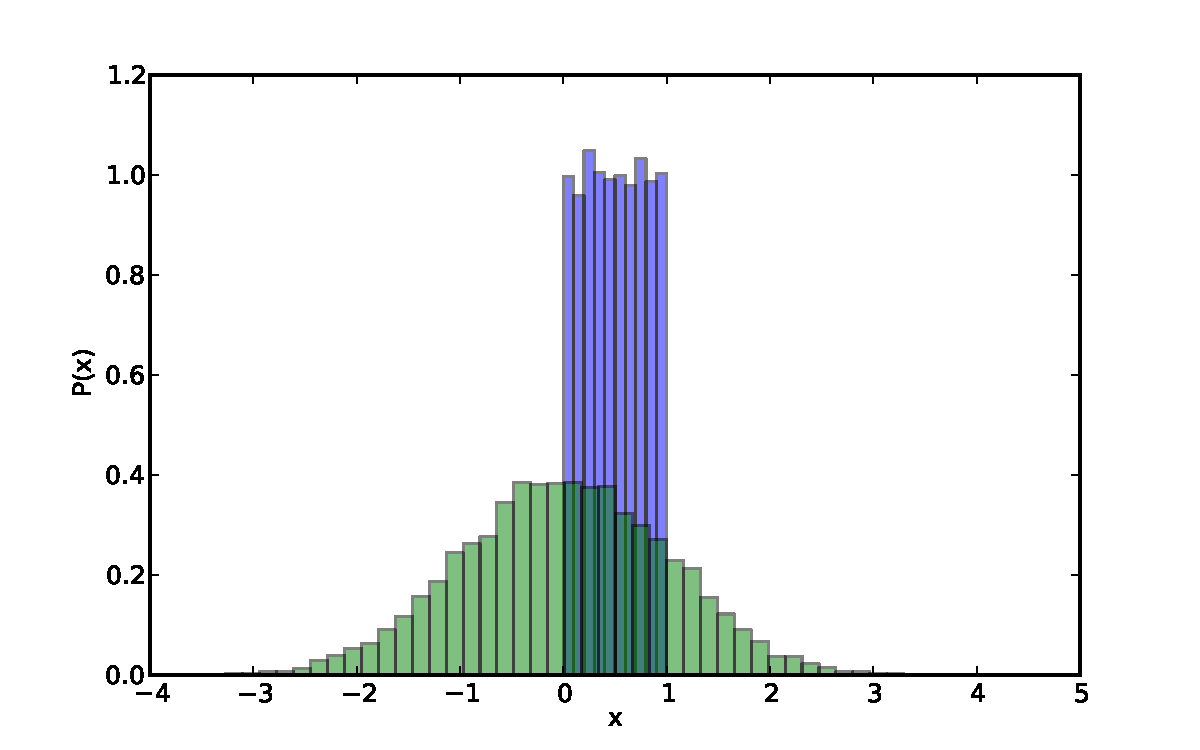
\includegraphics{randhistos.pdf}}
\caption{Histograms of random numbers.}\label{chap3/chap3_arrays:fig-randhistos}\end{figure}

If we want a random numbers with a Gaussian distribution of width \(\sigma\) centered about \(x_0\), we stretch the interval by a factor of \(\sigma\) and displace it by \(x_0\).  The following code produces 20 random numbers normally distributed around 15 with a width of 10:

\begin{Verbatim}[commandchars=\\\{\}]
\PYG{g+gp}{In [5]: }\PYG{n}{x0}\PYG{p}{,} \PYG{n}{sigma} \PYG{o}{=} \PYG{l+m+mi}{15}\PYG{p}{,} \PYG{l+m+mi}{10}

\PYG{g+gp}{In [6]: }\PYG{n}{sigma}\PYG{o}{*}\PYG{n}{randn}\PYG{p}{(}\PYG{l+m+mi}{20}\PYG{p}{)} \PYG{o}{+} \PYG{n}{x0}
\PYG{g+gr}{Out[6]: }\PYG{n}{array}\PYG{p}{(}\PYG{p}{[}  \PYG{l+m+mf}{9.36069244}\PYG{p}{,} \PYG{l+m+mf}{13.49260733}\PYG{p}{,}  \PYG{l+m+mf}{6.12550102}\PYG{p}{,}
\PYG{g+go}{                18.50471781,  9.89499319, 14.09576728,}
\PYG{g+go}{                12.45076637, 17.83073628,  2.95085564,}
\PYG{g+go}{                18.2756275 , 14.781659  , 31.80264078,}
\PYG{g+go}{                20.8457924 , 13.87890601, 25.41433678,}
\PYG{g+go}{                15.44237582, 21.2385386 , \PYGZhy{}3.91668973,}
\PYG{g+go}{                31.19120157, 26.24254326])}
\end{Verbatim}


\subsection{Random distribution of integers}
\label{chap3/chap3_arrays:random-distribution-of-integers}
The function \code{randint(low, high, num)} produces a uniform random distribution of \code{num} integers between \code{low} (inculsive) and \code{high} (exclsusive).  For example, we can simulate a dozen rolls a single die with the following statement

\begin{Verbatim}[commandchars=\\\{\}]
\PYG{g+gp}{In [7]: }\PYG{n}{randint}\PYG{p}{(}\PYG{l+m+mi}{1}\PYG{p}{,} \PYG{l+m+mi}{7}\PYG{p}{,} \PYG{l+m+mi}{12}\PYG{p}{)}
\PYG{g+gr}{Out[7]: }\PYG{n}{array}\PYG{p}{(}\PYG{p}{[}\PYG{l+m+mi}{6}\PYG{p}{,} \PYG{l+m+mi}{2}\PYG{p}{,} \PYG{l+m+mi}{1}\PYG{p}{,} \PYG{l+m+mi}{5}\PYG{p}{,} \PYG{l+m+mi}{4}\PYG{p}{,} \PYG{l+m+mi}{6}\PYG{p}{,} \PYG{l+m+mi}{3}\PYG{p}{,} \PYG{l+m+mi}{6}\PYG{p}{,} \PYG{l+m+mi}{5}\PYG{p}{,} \PYG{l+m+mi}{4}\PYG{p}{,} \PYG{l+m+mi}{6}\PYG{p}{,} \PYG{l+m+mi}{2}\PYG{p}{]}\PYG{p}{)}
\end{Verbatim}


\subsection{Loading random number functions}
\label{chap3/chap3_arrays:loading-random-number-functions}
When working within the IPython shell, you can use the random number functions simply by writing \code{rand(10)}, \code{randn(10)},  or, \code{randint(10)}, because the \code{np.random} library is loaded when IPython is launched.  However, to use these functions in a script or program, you need to load them from the \code{numpy.random} library, as discussed in section on {\hyperref[chap2/chap2_basics:importmods]{\emph{Importing Modules}}}, and as illustrated in the above program for making the histogram in the above figure.

\begin{tabulary}{\linewidth}{|L|}
\hline

\textbf{Recap of random number generators}
\\
\hline\end{tabulary}

\begin{quote}
\begin{description}
\item[{Random number generators}] \leavevmode
must be imported from the \code{numpy.random} library.  For more information, see \href{http://docs.scipy.org/doc/numpy/reference/routines.random.html}{http://docs.scipy.org/doc/numpy/reference/routines.random.html}

\item[{\code{rand(num)}}] \leavevmode
generates an array of \code{num} random floats uniformly distributed on the interval from 0 to 1.

\item[{\code{randn(num)}}] \leavevmode
generates an array of \code{num} random floats normally distributed with a width of 1.

\item[{\code{randint(low, high, num)}}] \leavevmode
generates an array of \code{num} random integers between \code{low} (inclusive) and \code{high} exclusive.

\end{description}
\end{quote}
\newpage

\section{Exercises}
\label{chap3/chap3_arrays:exercises}\begin{enumerate}
\item {} 
Create at array of 9 evenly spaced numbers going from 0 to 29 (inclusive) and give it the variable name \code{r}.  Find the square of each element of the array (as simply as possible).  Find twice the value of each element of the array in two different ways: (\emph{i}) using addition and (\emph{ii}) using multiplication.

\item {} 
Create the following arrays:
\begin{enumerate}
\item {} 
an array of 100 elements all equal to \(e\), the base of the natural logarithm;

\item {} 
an array in 1-degree increments of all the angles in degrees from 0 to 360 degrees;

\item {} 
an array in 1-degree increments of all the angles in radians from 0 to 360 degrees;

\item {} 
an array from 12 to 17, not including 17, in 0.2 increments;

\item {} 
an array from 12 to 17, including 17, in 0.2 increments.

\end{enumerate}

\item {} 
The position of a ball at time \(t\) dropped with zero initial velocity from a height \(h_0\) is given by
\begin{gather}
\begin{split}y = h_0 - \tfrac{1}{2}gt^2\end{split}\notag
\end{gather}
where \(g=9.8~\mathrm{m/s}^2\).  Suppose \(h_0=10~\mathrm{m}\).  Find the sequence of times when the ball passes each half meter assuming the ball is dropped at \(t=0\).  Hint: Create a NumPy array for \(y\) that goes from 10 to 0 in increments of -0.5 using the \code{arange} function.  Solving the above equation for \(t\), show that
\begin{gather}
\begin{split}t = \sqrt{\frac{2(h_0-y)}{g}} \;.\end{split}\notag
\end{gather}
Using this equation and the array you created, find the sequence of times when the ball passes each half meter.  Save your code as a Python script.  It should yield the following results for the \code{y} and \code{t} arrays:

\begin{Verbatim}[commandchars=\\\{\}]
\PYG{g+gp}{In [2]: }\PYG{n}{y}
\PYG{g+gr}{Out[2]: }\PYG{n}{array}\PYG{p}{(}\PYG{p}{[}\PYG{l+m+mf}{10.} \PYG{p}{,} \PYG{l+m+mf}{9.5}\PYG{p}{,} \PYG{l+m+mf}{9.} \PYG{p}{,} \PYG{l+m+mf}{8.5}\PYG{p}{,} \PYG{l+m+mf}{8.} \PYG{p}{,} \PYG{l+m+mf}{7.5}\PYG{p}{,} \PYG{l+m+mf}{7.} \PYG{p}{,} \PYG{l+m+mf}{6.5}\PYG{p}{,}
\PYG{g+go}{                6. , 5.5, 5. , 4.5, 4. , 3.5, 3. , 2.5,}
\PYG{g+go}{                2. , 1.5, 1. , 0.5])}

\PYG{g+gp}{In [3]: }\PYG{n}{t}
\PYG{g+gr}{Out[3]: }\PYG{n}{array}\PYG{p}{(}\PYG{p}{[} \PYG{l+m+mf}{0.}        \PYG{p}{,} \PYG{l+m+mf}{0.31943828}\PYG{p}{,} \PYG{l+m+mf}{0.45175395}\PYG{p}{,}
\PYG{g+go}{                0.55328334, 0.63887656, 0.71428571,}
\PYG{g+go}{                0.7824608 , 0.84515425, 0.9035079 ,}
\PYG{g+go}{                0.95831485, 1.01015254, 1.05945693,}
\PYG{g+go}{                1.10656667, 1.15175111, 1.19522861,}
\PYG{g+go}{                1.23717915, 1.27775313, 1.31707778,}
\PYG{g+go}{                1.35526185, 1.39239919])}
\end{Verbatim}

\item {} 
Recalling that the average velocity over an interval \(\Delta t\) is defined as \(\bar{v} = \Delta y/\Delta t\), find the average velocity for each time interval in the previous problem using NumPy arrays.  Keep in mind that the number of time intervals is one less than the number of times.  Hint: What are the arrays \code{y{[}1:20{]}} and \code{y{[}0:19{]}}?  What does the array \code{y{[}1:20{]}-y{[}0:19{]}} represent?  (Try printing out the two arrays from the IPython shell.) Using this last array and a similar one involving time, find the array of average velocities.  Bonus: Can you think of a more elegant way of representing \code{y{[}1:20{]}-y{[}0:19{]}} that does not make explicit reference to the number of elements in the \code{y} array---one that would work for any length array?

\end{enumerate}
\begin{quote}

You should get the following answer for the array of velocities:
\begin{quote}

\begin{Verbatim}[commandchars=\\\{\}]
\PYG{g+gp}{In [5]: }\PYG{n}{v}
\PYG{g+gr}{Out[5]: }\PYG{n}{array}\PYG{p}{(}\PYG{p}{[}\PYG{o}{\PYGZhy{}}\PYG{l+m+mf}{1.56524758}\PYG{p}{,}  \PYG{o}{\PYGZhy{}}\PYG{l+m+mf}{3.77884195}\PYG{p}{,}  \PYG{o}{\PYGZhy{}}\PYG{l+m+mf}{4.9246827} \PYG{p}{,}
\PYG{g+go}{               \PYGZhy{}5.84158351,  \PYGZhy{}6.63049517,  \PYGZhy{}7.3340579 ,}
\PYG{g+go}{               \PYGZhy{}7.97531375,  \PYGZhy{}8.56844457,  \PYGZhy{}9.12293148,}
\PYG{g+go}{               \PYGZhy{}9.64549022,  \PYGZhy{}10.14108641, \PYGZhy{}10.61351563,}
\PYG{g+go}{               \PYGZhy{}11.06575711, \PYGZhy{}11.50020061, \PYGZhy{}11.91879801,}
\PYG{g+go}{               \PYGZhy{}12.32316816, \PYGZhy{}12.71467146, \PYGZhy{}13.09446421,}
\PYG{g+go}{               \PYGZhy{}13.46353913])}
\end{Verbatim}
\end{quote}
\end{quote}


\chapter{Input and Output}
\label{chap4/chap4_io:input-and-output}\label{chap4/chap4_io:chap4}\label{chap4/chap4_io::doc}
\index{input}\index{output}
A good relationship depends on good communication.  In this chapter you learn how to communicate with Python.  Of course, communicating is a two-way street: input and output.  Generally, when you have Python perform some task, you need to feed it information---input.  When it is done with that task, it reports back to you the results of its calculations---output.

There are two venues for input that concern us: the computer keyboard and the input data file.  Similarly, there are two venues for output: the computer screen and the output data file.  We start with input from the keyboard and output to the computer screen.  Then we deal with data file input and output---or ``io.''

\index{input!keyboard}

\section{Keyboard input}
\label{chap4/chap4_io:keyboard-input}\label{chap4/chap4_io:index-1}
Many computer programs need input from the user.  In {\hyperref[chap2/chap2_basics:chap2-scriptexmp1]{\emph{Scripting Example 1}}}, the program needed the distance traveled as an input in order to determine the duration of the trip and the cost of the gasoline.  As you might like to use this same script to determine the cost of several different trips, it would be useful if the program requested that input when it was run from the IPython shell.

Python has a function called \code{raw\_input} (renamed \code{input} in Python 3) for getting input from the user and assigning it a variable name.  It has the form

\begin{Verbatim}[commandchars=\\\{\}]
\PYG{n}{strname} \PYG{o}{=} \PYG{n+nb}{raw\PYGZus{}input}\PYG{p}{(}\PYG{l+s}{\PYGZdq{}}\PYG{l+s}{prompt to user}\PYG{l+s}{\PYGZdq{}}\PYG{p}{)}
\end{Verbatim}

When the \code{raw\_input} statement is executed, it prints the text in the quotes to the computer screen and waits for input from the user.  The user types a string of characters and presses the return key.  The \code{raw\_input} function then assigns that string to the variable name on the right of the assignment operator \code{=}.

Let's try it out this snippet of code in the IPython shell.

\begin{Verbatim}[commandchars=\\\{\}]
\PYG{g+gp}{In [1]: }\PYG{n}{distance} \PYG{o}{=} \PYG{n+nb}{raw\PYGZus{}input}\PYG{p}{(}\PYG{l+s}{\PYGZdq{}}\PYG{l+s}{Input distance of trip in miles: }\PYG{l+s}{\PYGZdq{}}\PYG{p}{)}

\PYG{g+go}{Input distance of trip in miles:}
\end{Verbatim}

Python prints out the string argument of the \code{raw\_input} function and waits for a response from you.  Let's go ahead and type \code{450} for ``450 miles'' and press return.  Now type the variable name \code{distance} to see its value

\begin{Verbatim}[commandchars=\\\{\}]
\PYG{g+gp}{In [2]: }\PYG{n}{distance}
\PYG{g+gr}{Out[2]: }\PYG{l+s}{u\PYGZsq{}}\PYG{l+s}{450}\PYG{l+s}{\PYGZsq{}}
\end{Verbatim}

The value of the \code{distance} is \code{450} as expected, but it is a string (the \code{u} stands for ``unicode'' which refers to the string coding system Python uses).  Because we want to use \code{450} as a number and not a distance, we need to convert it from a string to a number.  We can do that with the \code{eval} function by writing

\begin{Verbatim}[commandchars=\\\{\}]
\PYG{g+gp}{In [3]: }\PYG{n}{distance} \PYG{o}{=} \PYG{n+nb}{eval}\PYG{p}{(}\PYG{n}{distance}\PYG{p}{)}

\PYG{g+gp}{In [4]: }\PYG{n}{distance}
\PYG{g+gr}{Out[4]: }\PYG{l+m+mi}{450}
\end{Verbatim}

The eval function has converted \emph{distance} to an integer.  This is fine and we are ready to move on.  However, we might prefer that \code{distance} be a float instead of an integer.  There are two ways to do this.  We could assume the user is very smart and will type ``\code{450.}'' instead of ``\code{450}'', which will cause distance to be a float when \code{eval} does the conversion.  That is, the number 450 is dynamically typed to be a float or an integer depending on whether or not the user uses a decimal point.  Alternatively, we could use the function \code{float} in place of \code{eval}, which would ensure that \code{distance} is a floating point variable.  Thus, our code would look like this (including the user response):

\begin{Verbatim}[commandchars=\\\{\}]
\PYG{g+gp}{In [5]: }\PYG{n}{distance} \PYG{o}{=} \PYG{n+nb}{raw\PYGZus{}input}\PYG{p}{(}\PYG{l+s}{\PYGZdq{}}\PYG{l+s}{Input distance of trip in miles: }\PYG{l+s}{\PYGZdq{}}\PYG{p}{)}

\PYG{g+go}{Input distance of trip in miles: 450}

\PYG{g+gp}{In [5]: }\PYG{n}{distance}
\PYG{g+gr}{Out[5]: }\PYG{l+s}{u\PYGZsq{}}\PYG{l+s}{450}\PYG{l+s}{\PYGZsq{}}

\PYG{g+gp}{In [7]: }\PYG{n}{distance} \PYG{o}{=} \PYG{n+nb}{float}\PYG{p}{(}\PYG{n}{distance}\PYG{p}{)}

\PYG{g+gp}{In [8]: }\PYG{n}{distance}
\PYG{g+gr}{Out[8]: }\PYG{l+m+mf}{450.0}
\end{Verbatim}

Now let's incorporate what we have learned into the code we wrote for {\hyperref[chap2/chap2_basics:chap2-scriptexmp1]{\emph{Scripting Example 1}}}

\begin{Verbatim}[commandchars=\\\{\},numbers=left,firstnumber=1,stepnumber=1]
\PYG{c}{\PYGZsh{} Calculates time, gallons of gas used, and cost of gasoline for}
\PYG{c}{\PYGZsh{} a trip}

\PYG{n}{distance} \PYG{o}{=} \PYG{n+nb}{raw\PYGZus{}input}\PYG{p}{(}\PYG{l+s}{\PYGZdq{}}\PYG{l+s}{Input distance of trip in miles: }\PYG{l+s}{\PYGZdq{}}\PYG{p}{)}
\PYG{n}{distance} \PYG{o}{=} \PYG{n+nb}{float}\PYG{p}{(}\PYG{n}{distance}\PYG{p}{)}

\PYG{n}{mpg} \PYG{o}{=} \PYG{l+m+mf}{30.}               \PYG{c}{\PYGZsh{} car mileage}
\PYG{n}{speed} \PYG{o}{=} \PYG{l+m+mf}{60.}             \PYG{c}{\PYGZsh{} average speed}
\PYG{n}{costPerGallon} \PYG{o}{=} \PYG{l+m+mf}{4.10}    \PYG{c}{\PYGZsh{} price of gas}

\PYG{n}{time} \PYG{o}{=} \PYG{n}{distance}\PYG{o}{/}\PYG{n}{speed}
\PYG{n}{gallons} \PYG{o}{=} \PYG{n}{distance}\PYG{o}{/}\PYG{n}{mpg}
\PYG{n}{cost} \PYG{o}{=} \PYG{n}{gallons}\PYG{o}{*}\PYG{n}{costPerGallon}
\end{Verbatim}

Lines 4 and 5 can be combined into a single line, which is a little more efficient:

\begin{Verbatim}[commandchars=\\\{\}]
\PYG{n}{distance} \PYG{o}{=} \PYG{n+nb}{float}\PYG{p}{(}\PYG{n+nb}{raw\PYGZus{}input}\PYG{p}{(}\PYG{l+s}{\PYGZdq{}}\PYG{l+s}{Input distance of trip in miles: }\PYG{l+s}{\PYGZdq{}}\PYG{p}{)}\PYG{p}{)}
\end{Verbatim}

Whether you use \code{float} or \code{int} or \code{eval} depends on whether you want a float, an integer, or a dynamically typed variable.  In this program, it doesn't matter.

Now you can simply run the program and then type \code{time}, \code{gallons}, and \code{cost} to view the results of the calculations done by the program.

Before moving on to output, we note that sometimes you may want string input rather that numerical input.  For example, you might want the user to input their name, in which case you would simply use the \code{raw\_input} function without converting its output.

\index{output!screen}

\section{Screen output}
\label{chap4/chap4_io:screen-output}\label{chap4/chap4_io:index-2}\label{chap4/chap4_io:screenoutput}
It would be much more convenient if the program in the previous section would simply write its output to the computer screen, instead of requiring the user to type \code{time}, \code{gallons}, and \code{cost} to view the results.  Fortunately, this can be accomplished very simply using Python's \code{print} function.  For example, simply including the statement \code{print(time, gallons, cost)} after line 12, running the program would give the following result:

\begin{Verbatim}[commandchars=\\\{\}]
\PYG{g+gp}{In [1]: }\PYG{n}{run} \PYG{n}{myTripIO}\PYG{o}{.}\PYG{n}{py}

\PYG{g+go}{What is the distance of your trip in miles? 450}
\PYG{g+go}{(7.5, 15.0, 61.49999999999999)}
\end{Verbatim}

The program prints out the results as a tuple of time (in hours), gasoline used (in gallons), and cost (in dollars).  Of course, the program doesn't give the user a clue as to which quantity is which.  The user has to know.


\subsection{Formatting output with \texttt{str.format()}}
\label{chap4/chap4_io:formatting-output-with-str-format}
We can clean up the output of the example above and make it considerably more user friendly.  The program below demonstrates how to do this.

\begin{Verbatim}[commandchars=\\\{\},numbers=left,firstnumber=1,stepnumber=1]
\PYG{c}{\PYGZsh{} Calculates time, gallons of gas used, and cost of gasoline for}
\PYG{c}{\PYGZsh{} a trip}

\PYG{n}{distance} \PYG{o}{=} \PYG{n+nb}{float}\PYG{p}{(}\PYG{n+nb}{raw\PYGZus{}input}\PYG{p}{(}\PYG{l+s}{\PYGZdq{}}\PYG{l+s}{Input distance of trip in miles: }\PYG{l+s}{\PYGZdq{}}\PYG{p}{)}\PYG{p}{)}
\PYG{n}{mpg} \PYG{o}{=} \PYG{l+m+mf}{30.}               \PYG{c}{\PYGZsh{} car mileage}
\PYG{n}{speed} \PYG{o}{=} \PYG{l+m+mf}{60.}             \PYG{c}{\PYGZsh{} average speed}
\PYG{n}{costPerGallon} \PYG{o}{=} \PYG{l+m+mf}{4.10}    \PYG{c}{\PYGZsh{} price of gas}

\PYG{n}{time} \PYG{o}{=} \PYG{n}{distance}\PYG{o}{/}\PYG{n}{speed}
\PYG{n}{gallons} \PYG{o}{=} \PYG{n}{distance}\PYG{o}{/}\PYG{n}{mpg}
\PYG{n}{cost} \PYG{o}{=} \PYG{n}{gallons}\PYG{o}{*}\PYG{n}{costPerGallon}

\PYG{k}{print}\PYG{p}{(}\PYG{l+s}{\PYGZdq{}}\PYG{l+s+se}{\PYGZbs{}n}\PYG{l+s}{Duration of trip = \PYGZob{}0:0.1f\PYGZcb{} hours}\PYG{l+s}{\PYGZdq{}}\PYG{o}{.}\PYG{n}{format}\PYG{p}{(}\PYG{n}{time}\PYG{p}{)}\PYG{p}{)}
\PYG{k}{print}\PYG{p}{(}\PYG{l+s}{\PYGZdq{}}\PYG{l+s}{Gasoline used = \PYGZob{}0:0.1f\PYGZcb{} gallons (@ \PYGZob{}1:0.0f\PYGZcb{} mpg)}\PYG{l+s}{\PYGZdq{}}
      \PYG{o}{.}\PYG{n}{format}\PYG{p}{(}\PYG{n}{gallons}\PYG{p}{,} \PYG{n}{mpg}\PYG{p}{)}\PYG{p}{)}
\PYG{k}{print}\PYG{p}{(}\PYG{l+s}{\PYGZdq{}}\PYG{l+s}{Cost of gasoline = \PYGZdl{}\PYGZob{}0:0.2f\PYGZcb{} (@ \PYGZdl{}\PYGZob{}1:0.2f\PYGZcb{}/gallon)}\PYG{l+s}{\PYGZdq{}}
      \PYG{o}{.}\PYG{n}{format}\PYG{p}{(}\PYG{n}{cost}\PYG{p}{,} \PYG{n}{costPerGallon}\PYG{p}{)}\PYG{p}{)}
\end{Verbatim}

The final two \code{print} function calls in this script are continued on a second line in order to improve readability.
Running this program, with the distance provided by the user, gives

\begin{Verbatim}[commandchars=\\\{\}]
\PYG{g+gp}{In [9]: }\PYG{n}{run} \PYG{n}{myTripNiceIO}\PYG{o}{.}\PYG{n}{py}

\PYG{g+go}{What is the trip distance in miles? 450}

\PYG{g+go}{Duration of trip = 7.5 hours}
\PYG{g+go}{Gasoline used = 15.0 gallons (@ 30 mpg)}
\PYG{g+go}{Cost of gasoline = \PYGZdl{}61.50 (@ \PYGZdl{}4.10/gallon)}
\end{Verbatim}

Now the output is presented in a way that is immediately understandable to the user.  Moreover, the numerical output is formatted with an appropriate number of digits to the right of the decimal point.  For good measure, we also included the assumed mileage (30 mpg) and the cost of the gasoline.  All of this is controlled by the \code{str.format()} function within the \code{print} function.

The argument of the \code{print} function is of the form \code{str.format()} where  \code{str} is a string that contains text that is written to be the screen, as well as certain format specifiers contained in curly braces \code{\{\}}.  The \code{format} function contains the list of variables that are to be printed.
\begin{itemize}
\item {} 
The \code{\textbackslash{}n} at the start of the string in the \code{print} statement on line 12 in the newline character.  It creates the blank line before the output is printed.

\item {} 
The positions of the curly braces determine where the variables in the \code{format} function at the end of the statement are printed.

\item {} 
The format string inside the curly braces specifies how each variable in the \code{format} function is printed.

\item {} 
The number before the colon in the format string specifies which variable in the list in the \code{format} function is printed.  Remember, Python is zero-indexed, so 0 means the first variable is printed, 1 means the second variable, \emph{etc}.

\item {} 
The zero after the colon specifies the \emph{minimum} number of spaces reserved for printing out the variable in the format function. A zero means that only as many spaces as needed will be used.

\item {} 
The number after the period specifies the number of digits to the right of the decimal point that will be printed: \code{1} for \code{time} and \code{gallons} and \code{2} for \code{cost}.

\item {} 
The \code{f} specifies that a number with a fixed number of decimal points.  If the \code{f} format specifier is replaced with \code{e}, then the number is printed out in exponential format (scientific notation).

\end{itemize}

In addition to \code{f} and \code{e} format types, there are two more that are commonly used: \code{d} for integers (digits) and \code{s} for strings.  There are, in fact, many more formatting possibilities.  Python has a whole ``Format Specification Mini-Language'' that is documented at \href{http://docs.python.org/library/string.html\#formatspec}{http://docs.python.org/library/string.html\#formatspec}.  It's very flexible but arcane.  You might find it simplest to look at the ``Format examples'' section further down the same web page.

The program below illustrates most of the formatting you will need for writing a few variables, be they strings, integers, or floats, to screen or to data files (which we discuss in the next section).

\begin{Verbatim}[commandchars=\\\{\}]
\PYG{n}{string1} \PYG{o}{=} \PYG{l+s}{\PYGZdq{}}\PYG{l+s}{How}\PYG{l+s}{\PYGZdq{}}
\PYG{n}{string2} \PYG{o}{=} \PYG{l+s}{\PYGZdq{}}\PYG{l+s}{are you my friend?}\PYG{l+s}{\PYGZdq{}}
\PYG{n}{int1} \PYG{o}{=} \PYG{l+m+mi}{34}
\PYG{n}{int2} \PYG{o}{=} \PYG{l+m+mi}{942885}
\PYG{n}{float1} \PYG{o}{=} \PYG{o}{\PYGZhy{}}\PYG{l+m+mf}{3.0}
\PYG{n}{float2} \PYG{o}{=} \PYG{l+m+mf}{3.141592653589793e\PYGZhy{}14}

\PYG{k}{print}\PYG{p}{(}\PYG{l+s}{\PYGZsq{}}\PYG{l+s}{ ***}\PYG{l+s}{\PYGZsq{}}\PYG{p}{)}
\PYG{k}{print}\PYG{p}{(}\PYG{n}{string1}\PYG{p}{)}
\PYG{k}{print}\PYG{p}{(}\PYG{n}{string1} \PYG{o}{+} \PYG{l+s}{\PYGZsq{}}\PYG{l+s}{ }\PYG{l+s}{\PYGZsq{}} \PYG{o}{+} \PYG{n}{string2}\PYG{p}{)}
\PYG{k}{print}\PYG{p}{(}\PYG{l+s}{\PYGZsq{}}\PYG{l+s}{ 1. \PYGZob{}\PYGZcb{} \PYGZob{}\PYGZcb{}}\PYG{l+s}{\PYGZsq{}}\PYG{o}{.}\PYG{n}{format}\PYG{p}{(}\PYG{n}{string1}\PYG{p}{,} \PYG{n}{string2}\PYG{p}{)}\PYG{p}{)}
\PYG{k}{print}\PYG{p}{(}\PYG{l+s}{\PYGZsq{}}\PYG{l+s}{ 2. \PYGZob{}0:s\PYGZcb{} \PYGZob{}1:s\PYGZcb{}}\PYG{l+s}{\PYGZsq{}}\PYG{o}{.}\PYG{n}{format}\PYG{p}{(}\PYG{n}{string1}\PYG{p}{,} \PYG{n}{string2}\PYG{p}{)}\PYG{p}{)}
\PYG{k}{print}\PYG{p}{(}\PYG{l+s}{\PYGZsq{}}\PYG{l+s}{ 3. \PYGZob{}0:s\PYGZcb{} \PYGZob{}0:s\PYGZcb{} \PYGZob{}1:s\PYGZcb{} \PYGZhy{} \PYGZob{}0:s\PYGZcb{} \PYGZob{}1:s\PYGZcb{}}\PYG{l+s}{\PYGZsq{}}
      \PYG{o}{.}\PYG{n}{format}\PYG{p}{(}\PYG{n}{string1}\PYG{p}{,} \PYG{n}{string2}\PYG{p}{)}\PYG{p}{)}
\PYG{k}{print}\PYG{p}{(}\PYG{l+s}{\PYGZsq{}}\PYG{l+s}{ 4. \PYGZob{}0:10s\PYGZcb{}\PYGZob{}1:5s\PYGZcb{}}\PYG{l+s}{\PYGZsq{}}
      \PYG{o}{.}\PYG{n}{format}\PYG{p}{(}\PYG{n}{string1}\PYG{p}{,} \PYG{n}{string2}\PYG{p}{)}\PYG{p}{)}
\PYG{k}{print}\PYG{p}{(}\PYG{l+s}{\PYGZsq{}}\PYG{l+s}{ ***}\PYG{l+s}{\PYGZsq{}}\PYG{p}{)}
\PYG{k}{print}\PYG{p}{(}\PYG{n}{int1}\PYG{p}{,} \PYG{n}{int2}\PYG{p}{)}
\PYG{k}{print}\PYG{p}{(}\PYG{l+s}{\PYGZsq{}}\PYG{l+s}{ 6. \PYGZob{}0:d\PYGZcb{} \PYGZob{}1:d\PYGZcb{}}\PYG{l+s}{\PYGZsq{}}\PYG{o}{.}\PYG{n}{format}\PYG{p}{(}\PYG{n}{int1}\PYG{p}{,} \PYG{n}{int2}\PYG{p}{)}\PYG{p}{)}
\PYG{k}{print}\PYG{p}{(}\PYG{l+s}{\PYGZsq{}}\PYG{l+s}{ 7. \PYGZob{}0:8d\PYGZcb{} \PYGZob{}1:10d\PYGZcb{}}\PYG{l+s}{\PYGZsq{}}\PYG{o}{.}\PYG{n}{format}\PYG{p}{(}\PYG{n}{int1}\PYG{p}{,} \PYG{n}{int2}\PYG{p}{)}\PYG{p}{)}
\PYG{k}{print}\PYG{p}{(}\PYG{l+s}{\PYGZsq{}}\PYG{l+s}{ ***}\PYG{l+s}{\PYGZsq{}}\PYG{p}{)}
\PYG{k}{print}\PYG{p}{(}\PYG{l+s}{\PYGZsq{}}\PYG{l+s}{ 8. \PYGZob{}0:0.3f\PYGZcb{}}\PYG{l+s}{\PYGZsq{}}\PYG{o}{.}\PYG{n}{format}\PYG{p}{(}\PYG{n}{float1}\PYG{p}{)}\PYG{p}{)}
\PYG{k}{print}\PYG{p}{(}\PYG{l+s}{\PYGZsq{}}\PYG{l+s}{ 9. \PYGZob{}0:6.3f\PYGZcb{}}\PYG{l+s}{\PYGZsq{}}\PYG{o}{.}\PYG{n}{format}\PYG{p}{(}\PYG{n}{float1}\PYG{p}{)}\PYG{p}{)}
\PYG{k}{print}\PYG{p}{(}\PYG{l+s}{\PYGZsq{}}\PYG{l+s}{10. \PYGZob{}0:8.3f\PYGZcb{}}\PYG{l+s}{\PYGZsq{}}\PYG{o}{.}\PYG{n}{format}\PYG{p}{(}\PYG{n}{float1}\PYG{p}{)}\PYG{p}{)}
\PYG{k}{print}\PYG{p}{(}\PYG{l+m+mi}{2}\PYG{o}{*}\PYG{l+s}{\PYGZsq{}}\PYG{l+s}{11. \PYGZob{}0:8.3f\PYGZcb{}}\PYG{l+s}{\PYGZsq{}}\PYG{o}{.}\PYG{n}{format}\PYG{p}{(}\PYG{n}{float1}\PYG{p}{)}\PYG{p}{)}
\PYG{k}{print}\PYG{p}{(}\PYG{l+s}{\PYGZsq{}}\PYG{l+s}{ ***}\PYG{l+s}{\PYGZsq{}}\PYG{p}{)}
\PYG{k}{print}\PYG{p}{(}\PYG{l+s}{\PYGZsq{}}\PYG{l+s}{12. \PYGZob{}0:0.3e\PYGZcb{}}\PYG{l+s}{\PYGZsq{}}\PYG{o}{.}\PYG{n}{format}\PYG{p}{(}\PYG{n}{float2}\PYG{p}{)}\PYG{p}{)}
\PYG{k}{print}\PYG{p}{(}\PYG{l+s}{\PYGZsq{}}\PYG{l+s}{13. \PYGZob{}0:10.3e\PYGZcb{}}\PYG{l+s}{\PYGZsq{}}\PYG{o}{.}\PYG{n}{format}\PYG{p}{(}\PYG{n}{float2}\PYG{p}{)}\PYG{p}{)}
\PYG{k}{print}\PYG{p}{(}\PYG{l+s}{\PYGZsq{}}\PYG{l+s}{14. \PYGZob{}0:10.3f\PYGZcb{}}\PYG{l+s}{\PYGZsq{}}\PYG{o}{.}\PYG{n}{format}\PYG{p}{(}\PYG{n}{float2}\PYG{p}{)}\PYG{p}{)}
\PYG{k}{print}\PYG{p}{(}\PYG{l+s}{\PYGZsq{}}\PYG{l+s}{ ***}\PYG{l+s}{\PYGZsq{}}\PYG{p}{)}
\PYG{k}{print}\PYG{p}{(}\PYG{l+s}{\PYGZsq{}}\PYG{l+s}{15. 12345678901234567890}\PYG{l+s}{\PYGZsq{}}\PYG{p}{)}
\PYG{k}{print}\PYG{p}{(}\PYG{l+s}{\PYGZsq{}}\PYG{l+s}{16. \PYGZob{}0:s\PYGZcb{}\PYGZhy{}\PYGZhy{}\PYGZob{}1:8d\PYGZcb{},\PYGZob{}2:10.3e\PYGZcb{}}\PYG{l+s}{\PYGZsq{}}
      \PYG{o}{.}\PYG{n}{format}\PYG{p}{(}\PYG{n}{string2}\PYG{p}{,} \PYG{n}{int1}\PYG{p}{,} \PYG{n}{float2}\PYG{p}{)}\PYG{p}{)}
\end{Verbatim}

Here is the output:

\begin{Verbatim}[commandchars=\\\{\},numbers=left,firstnumber=1,stepnumber=1]
 ***
How
How are you my friend?
 1. How are you my friend?
 2. How are you my friend?
 3. How How are you my friend? \PYGZhy{} How are you my friend?
 4. How       are you my friend?
 ***
(34, 942885)
 6. 34 942885
 7.       34     942885
 ***
 8. \PYGZhy{}3.000
 9. \PYGZhy{}3.000
10.   \PYGZhy{}3.000
11.   \PYGZhy{}3.00011.   \PYGZhy{}3.000
 ***
12. 3.142e\PYGZhy{}14
13.  3.142e\PYGZhy{}14
14.      0.000
 ***
15. 12345678901234567890
16. are you my friend?\PYGZhy{}\PYGZhy{}      34, 3.142e\PYGZhy{}14
\end{Verbatim}

Successive empty brackets \code{\{\}} like those that appear in the statement above \code{print(' 1. \{\} \{\}'.format(string1, string2))} are numbered consecutively starting at 0 and will print out whatever variables appear inside the \code{format()} method using their default format.

Finally, note that the code starting on lines 14 and 16 each are split into two lines.  We have done this so that the lines fit on the page without running off the edge.  Python allows you to break lines up like this to improve readability.


\subsection{Printing arrays}
\label{chap4/chap4_io:printing-arrays}
\index{array (NumPy)!printing}
Formatting NumPy arrays for printing requires another approach.  As an example, let's create an array and then format it in various ways.  From the IPython terminal

\begin{Verbatim}[commandchars=\\\{\}]
\PYG{g+gp}{In [10]: }\PYG{n}{a} \PYG{o}{=} \PYG{n}{linspace}\PYG{p}{(}\PYG{l+m+mi}{3}\PYG{p}{,} \PYG{l+m+mi}{19}\PYG{p}{,} \PYG{l+m+mi}{7}\PYG{p}{)}
\PYG{g+gp}{In [11]: }\PYG{k}{print}\PYG{p}{(}\PYG{n}{a}\PYG{p}{)}
\PYG{g+go}{[  3.           5.66666667   8.33333333  11.}
\PYG{g+go}{   13.66666667  16.33333333  19.        ]}
\end{Verbatim}

Simply using the \code{print} function does print out the array, but perhaps not in the format you desire.  To control the output format, you use the NumPy function \code{set\_printoptions}.  For example, suppose you want to see no more than two digits to the right of the decimal point.  Then you simply write

\begin{Verbatim}[commandchars=\\\{\}]
\PYG{g+gp}{In [12]: }\PYG{n}{set\PYGZus{}printoptions}\PYG{p}{(}\PYG{n}{precision}\PYG{o}{=}\PYG{l+m+mi}{2}\PYG{p}{)}
\PYG{g+gp}{In [13]: }\PYG{k}{print}\PYG{p}{(}\PYG{n}{a}\PYG{p}{)}
\PYG{g+go}{[  3.     5.67   8.33  11.    13.67  16.33  19.  ]}
\end{Verbatim}

If you want to change the number of digits to the right of the decimal point to 4, you set the keyword argument \code{precision} to 4

\begin{Verbatim}[commandchars=\\\{\}]
\PYG{g+gp}{In [14]: }\PYG{n}{set\PYGZus{}printoptions}\PYG{p}{(}\PYG{n}{precision}\PYG{o}{=}\PYG{l+m+mi}{4}\PYG{p}{)}
\PYG{g+gp}{In [15]: }\PYG{k}{print}\PYG{p}{(}\PYG{n}{a}\PYG{p}{)}
\PYG{g+go}{[  3.       5.6667   8.3333  11.      13.6667  16.3333  19.    ]}
\end{Verbatim}

Suppose you want to use scientific notation.  The method for doing it is somewhat arcane, using something called a \code{lambda} function.  For now, you don't need to understand how it works to use it.  Just follow the examples shown below, which illustrate several different output formats using the \code{print} function with NumPy arrays.

\begin{Verbatim}[commandchars=\\\{\}]
\PYG{g+gp}{In [16]: }\PYG{n}{set\PYGZus{}printoptions}\PYG{p}{(}
\PYG{g+go}{    ...: formatter=\PYGZob{}\PYGZsq{}float\PYGZsq{}: lambda x: format(x, \PYGZsq{}6.2e\PYGZsq{})\PYGZcb{})}

\PYG{g+gp}{In [17]: }\PYG{k}{print}\PYG{p}{(}\PYG{n}{a}\PYG{p}{)}
\PYG{g+go}{[3.00e+00 5.67e+00 8.33e+00 1.10e+01 1.37e+01 1.63e+01 1.90e+01]}
\end{Verbatim}

To specify the format of the output, you use the \code{formatter} keyword argument.  The first entry to the right of the curly bracket is a string that can be \code{'float'}, as it is above, or \code{'int'}, or \code{'str'}, or a number of other data types that you can look up in the online NumPy documentation.  The only other thing you should change is the format specifier string.  In the above example, it is \code{'6.2e'}, specifying that Python should allocate at least 6 spaces, with 2 digits to the right of the decimal point in scientific (exponential) notation.  For fixed width floats with 3 digits to the right of the decimal point, use the \code{f} in place of the \code{e} format specifier, as follows

\begin{Verbatim}[commandchars=\\\{\}]
\PYG{g+gp}{In [18]: }\PYG{n}{set\PYGZus{}printoptions}\PYG{p}{(}
\PYG{g+go}{    ...: formatter=\PYGZob{}\PYGZsq{}float\PYGZsq{}: lambda x: format(x, \PYGZsq{}6.3f\PYGZsq{})\PYGZcb{})}
\PYG{g+gp}{In [19]: }\PYG{k}{print}\PYG{p}{(}\PYG{n}{a}\PYG{p}{)}
\PYG{g+go}{[ 3.000  5.667  8.333 11.000 13.667 16.333 19.000]}
\end{Verbatim}

To return to the default format, type the following

\begin{Verbatim}[commandchars=\\\{\}]
\PYG{g+gp}{In [20]: }\PYG{n}{set\PYGZus{}printoptions}\PYG{p}{(}\PYG{n}{precision}\PYG{o}{=}\PYG{l+m+mi}{8}\PYG{p}{)}
\PYG{g+gp}{In [21]: }\PYG{k}{print}\PYG{p}{(}\PYG{n}{a}\PYG{p}{)}
\PYG{g+go}{[  3.           5.66666667   8.33333333  11.}
\PYG{g+go}{   13.66666667  16.33333333  19.        ]}
\end{Verbatim}

The \code{set\_printoptions} is a NumPy function, so if you use it in a script or program, you should call it by writing \code{np.set\_printoptions}.

\index{input!reading data from a file}

\section{File input}
\label{chap4/chap4_io:index-4}\label{chap4/chap4_io:file-input}

\subsection{Reading data from a text file}
\label{chap4/chap4_io:reading-data-from-a-text-file}
Often you would like to analyze data that you have stored in a text file.  Consider, for example, the data file below for an experiment measuring the free fall of a mass.

\begin{Verbatim}[commandchars=\\\{\},numbers=left,firstnumber=1,stepnumber=1]
Data for falling mass experiment
Date: 16\PYGZhy{}Aug\PYGZhy{}2013
Data taken by Lauren and John

data point      time (sec)      height (mm)     uncertainty (mm)
    0               0.0             180             3.5
    1               0.5             182             4.5
    2               1.0             178             4.0
    3               1.5             165             5.5
    4               2.0             160             2.5
    5               2.5             148             3.0
    6               3.0             136             2.5
    7               3.5             120             3.0
    8               4.0              99             4.0
    9               4.5              83             2.5
   10               5.0              55             3.6
   11               5.5              35             1.75
   12               6.0               5             0.75
\end{Verbatim}

We would like to read these data into a Python program, associating the data in each column with an appropriately named array.  While there are a multitude of ways to do this in Python, the simplest by far is to use the NumPy \code{loadtxt} function, whose use we illustrate here.  Suppose that the name of the text file is \code{MyData.txt}.  Then we can read the data into four different arrays with the following statement

\begin{Verbatim}[commandchars=\\\{\}]
\PYG{g+gp}{In [1]: }\PYG{n}{dataPt}\PYG{p}{,} \PYG{n}{time}\PYG{p}{,} \PYG{n}{height}\PYG{p}{,} \PYG{n}{error} \PYG{o}{=} \PYG{n}{np}\PYG{o}{.}\PYG{n}{loadtxt}\PYG{p}{(}\PYG{l+s}{\PYGZdq{}}\PYG{l+s}{MyData.txt}\PYG{l+s}{\PYGZdq{}}\PYG{p}{,}
\PYG{g+go}{      skiprows=5 , unpack=True)}
\end{Verbatim}

In this case, the \code{loadtxt} function takes three arguments: the first is a string that is the name of the file to be read, the second tells \code{loadtxt} to skip the first 5 lines at the top of file, sometimes called the \emph{header}, and the third tells \code{loadtxt} to output the data (\emph{unpack} the data) so that it can be directly read into arrays.  \code{loadtxt} reads however many columns of data are present in the text file to the array names listed to the left of the ``\code{=}'' sign.  The names labeling the columns in the text file are not used, but you are free to choose the same or similar names, of course, as long as they are legal array names.  By the way, for the above \code{loadtxt} call to work, the file \code{MyData.txt} should be in the current working directory of the IPython shell. Otherwise, you need to specify the directory path with the file name.

It is critically important that the data file be a \emph{text} file.  It cannot be a MSWord file, for example, or an Excel file, or anything other than a plain text file.  Such files can be created by a text editor programs like \textbf{Notepad} and \textbf{Notepad++} (for a PC) or \textbf{TextEdit} and \textbf{TextWrangler} (for a Mac).  They can also be created by MSWord and Excel provided you explicitly save the files as text files.  \textbf{Beware}: You should exit any text file you make and save it with a program that allows you to save the text file using \textbf{UNIX}-type formatting, which uses a \emph{line feed} (LF) to end a line.  Some programs, like MSWord under Windows, may include a carriage return (CR) character, which can confuse \code{loadtxt}.  Note that we give the file name a \code{.txt} \emph{extension}, which indicates to most operating systems that this is a \emph{text} file, as opposed to an Excel file, for example, which might have a \code{.xlsx} or \code{.xls} extension.

If you don't want to read in all the columns of data, you can specify which columns to read in using the \code{usecols} key word.  For example, the call

\begin{Verbatim}[commandchars=\\\{\}]
\PYG{g+gp}{In [2]: }\PYG{n}{time}\PYG{p}{,} \PYG{n}{height} \PYG{o}{=} \PYG{n}{loadtxt}\PYG{p}{(}\PYG{l+s}{\PYGZsq{}}\PYG{l+s}{MyData.txt}\PYG{l+s}{\PYGZsq{}}\PYG{p}{,} \PYG{n}{skiprows}\PYG{o}{=}\PYG{l+m+mi}{5} \PYG{p}{,}
\PYG{g+go}{                                 usecols = (1,2), unpack=True)}
\end{Verbatim}

reads in only columns 1 and 2; columns 0 and 3 are skipped.  As a consequence, only two array names are included to the left of the ``\code{=}'' sign, corresponding to the two column that are read.  Writing \code{usecols = (0,2,3)} would skip column 1 and read in only the data in colums 0, 2, and 3.  In this case, 3 array names would need to be provided on the left hand side of the ``\code{=}'' sign.

One convenient feature of the \code{loadtxt} function is that it recognizes any \emph{white space} as a column separator: spaces, tabs, \emph{etc.}

Finally you should remember that \code{loadtxt} is a NumPy function.  So if you are using it in a Python module, you must be sure to include an ``\code{import numpy as np}''  statement before calling ``\code{np.loadtxt}''.


\subsection{Reading data from a CSV file}
\label{chap4/chap4_io:reading-data-from-a-csv-file}
Sometimes you have data stored in a spreadsheet program like Excel that you would like to read into a Python program.  The {\hyperref[chap4/chap4_io:fig-excelwindow]{\emph{Excel data sheet}}} shown here contains the same data set we saw above in a text file.
\begin{figure}[htbp]
\centering
\capstart

\scalebox{0.650000}{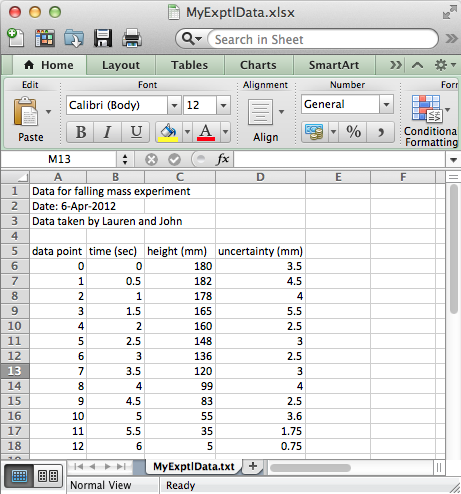
\includegraphics{ExcelDataFile.png}}
\caption{Excel data sheet}\label{chap4/chap4_io:fig-excelwindow}\end{figure}

While there are a number of different approaches one can use to reading such files, one of the simplest of most robust is to save the spreadsheet as a CSV (``comma separated value'') file, a format which all common spreadsheet programs can create and read.  So, if your Excel spreadsheet was called \code{MyData.xlsx}, the CSV file saved using Excel's \code{Save As} command would by default be \code{MyData.csv}.  It would look like this

\begin{Verbatim}[commandchars=\\\{\},numbers=left,firstnumber=1,stepnumber=1]
Data for falling mass experiment,,,
Date: 16\PYGZhy{}Aug\PYGZhy{}2013,,,
Data taken by Lauren and John,,,
,,,
data point,time (sec),height (mm),uncertainty (mm)
0,0,180,3.5
1,0.5,182,4.5
2,1,178,4
3,1.5,165,5.5
4,2,160,2.5
5,2.5,148,3
6,3,136,2.5
7,3.5,120,3
8,4,99,4
9,4.5,83,2.5
10,5,55,3.6
11,5.5,35,1.75
12,6,5,0.75
\end{Verbatim}

As its name suggests, the CSV file is simply a text file with the data that was formerly in spreadsheet columns now separated by commas.  We can read the data in this file into a Python program using the \code{loadtxt} NumPy function once again.  Here is the code

\begin{Verbatim}[commandchars=\\\{\}]
\PYG{g+gp}{In [3]: }\PYG{n}{dataPt}\PYG{p}{,} \PYG{n}{time}\PYG{p}{,} \PYG{n}{height}\PYG{p}{,} \PYG{n}{error} \PYG{o}{=} \PYG{n}{loadtxt}\PYG{p}{(}\PYG{l+s}{\PYGZdq{}}\PYG{l+s}{MyData.csv}\PYG{l+s}{\PYGZdq{}}\PYG{p}{,}
\PYG{g+go}{                      skiprows=5 , unpack=True, delimiter=\PYGZsq{},\PYGZsq{})}
\end{Verbatim}

The form of the function is exactly the same as before except we have added the argument \code{delimiter=','} that tells \code{loadtxt} that the columns are separated by commas instead of white space (spaces or tabs), which is the default.  Once again, we set the \code{skiprows} argument to skip the header at the beginning of the file and to start reading at the first row of data.  The data are output to the arrays to the right of the assignment operator \code{=} exactly as in the previous example.

\index{output!writing data to a file}

\section{File output}
\label{chap4/chap4_io:index-5}\label{chap4/chap4_io:file-output}

\subsection{Writing data to a text file}
\label{chap4/chap4_io:writing-data-to-a-text-file}
There is a plethora of ways to write data to a data file in Python.  We will stick to one very simple one that's suitable for writing data files in text format.  It uses the NumPy \code{savetxt} routine, which is the counterpart of the \code{loadtxt} routine introduced in the previous section.  The general form of the routine is

\begin{Verbatim}[commandchars=\\\{\}]
\PYG{n}{savetxt}\PYG{p}{(}\PYG{n}{filename}\PYG{p}{,} \PYG{n}{array}\PYG{p}{,} \PYG{n}{fmt}\PYG{o}{=}\PYG{l+s}{\PYGZdq{}}\PYG{l+s+si}{\PYGZpc{}0.18e}\PYG{l+s}{\PYGZdq{}}\PYG{p}{,} \PYG{n}{delimiter}\PYG{o}{=}\PYG{l+s}{\PYGZdq{}}\PYG{l+s}{ }\PYG{l+s}{\PYGZdq{}}\PYG{p}{,} \PYG{n}{newline}\PYG{o}{=}\PYG{l+s}{\PYGZdq{}}\PYG{l+s+se}{\PYGZbs{}n}\PYG{l+s}{\PYGZdq{}}\PYG{p}{,}
    \PYG{n}{header}\PYG{o}{=}\PYG{l+s}{\PYGZdq{}}\PYG{l+s}{\PYGZdq{}}\PYG{p}{,} \PYG{n}{footer}\PYG{o}{=}\PYG{l+s}{\PYGZdq{}}\PYG{l+s}{\PYGZdq{}}\PYG{p}{,} \PYG{n}{comments}\PYG{o}{=}\PYG{l+s}{\PYGZdq{}}\PYG{l+s}{\PYGZsh{} }\PYG{l+s}{\PYGZdq{}}\PYG{p}{)}
\end{Verbatim}

We illustrate \code{savetext} below with a script that first creates four arrays by reading in the data file \code{MyData.txt}, as discussed in the previous section, and then writes that same data set to another file \code{MyDataOut.txt}.

\begin{Verbatim}[commandchars=\\\{\},numbers=left,firstnumber=1,stepnumber=1]
\PYG{k+kn}{import} \PYG{n+nn}{numpy} \PYG{k+kn}{as} \PYG{n+nn}{np}

\PYG{n}{dataPt}\PYG{p}{,} \PYG{n}{time}\PYG{p}{,} \PYG{n}{height}\PYG{p}{,} \PYG{n}{error} \PYG{o}{=} \PYG{n}{np}\PYG{o}{.}\PYG{n}{loadtxt}\PYG{p}{(}\PYG{l+s}{\PYGZdq{}}\PYG{l+s}{MyData.txt}\PYG{l+s}{\PYGZdq{}}\PYG{p}{,}
                                 \PYG{n}{skiprows}\PYG{o}{=}\PYG{l+m+mi}{5}\PYG{p}{,} \PYG{n}{unpack}\PYG{o}{=}\PYG{n+nb+bp}{True}\PYG{p}{)}

\PYG{n}{np}\PYG{o}{.}\PYG{n}{savetxt}\PYG{p}{(}\PYG{l+s}{\PYGZsq{}}\PYG{l+s}{MyDataOut.txt}\PYG{l+s}{\PYGZsq{}}\PYG{p}{,}
    \PYG{n+nb}{zip}\PYG{p}{(}\PYG{n}{dataPt}\PYG{p}{,} \PYG{n}{time}\PYG{p}{,} \PYG{n}{height}\PYG{p}{,} \PYG{n}{error}\PYG{p}{)}\PYG{p}{,} \PYG{n}{fmt}\PYG{o}{=}\PYG{l+s}{\PYGZdq{}}\PYG{l+s+si}{\PYGZpc{}12.1f}\PYG{l+s}{\PYGZdq{}}\PYG{p}{)}
\end{Verbatim}

The first argument of of \code{savetxt} is a string, the name of the data file to be created.  Here we have chosen the name \code{MyDataOut.txt}, inserted with quotes, which designates it as a string literal.  Beware, if there is already a file of that name on your computer, it will be overwritten---the old file will be destroyed and a new one will be created.

The second argument is the data array the is to be written to the data file.  Because we want to write not one but four data arrays to the file, we have to package the four data arrays as one, which we do using the \code{zip} function, a Python function that combines returns a list of tuples, where the \(i^\mathrm{th}\) tuple contains the \(i^\mathrm{th}\) element from each of the arrays (or lists, or tuples) listed as its arguments.  Since there are four arrays, each row will be a tuple with four entries, producing a table with four columns.  Note that the first two arguments, the filename and data array, are regular arguments and thus must appear as the first and second arguments in the correct order.  The remaining arguments are all keyword arguments, meaning that they are optional and can appear in any order, provided you use the keyword.

The next argument is a format string that determines how the elements of the array are displayed in the data file.  The argument is optional and, if left out, is the format \code{0.18e}, which displays numbers as 18 digit floats in exponential (scientific) notation.  Here we choose a different format, \code{12.1f}, which is a float displayed with 1 digit to the right of the decimal point and a minimum width of 12.  By choosing 12, which is more digits than any of the numbers in the various arrays have, we ensure that all the columns will have the same width.  It also ensures that the decimal points in column of numbers are aligned.   This is evident in the data file below, \emph{MyDataOut.txt}, which was produced by the above script.

\begin{Verbatim}[commandchars=\\\{\}]
 \PYG{l+m+mf}{0.0}          \PYG{l+m+mf}{0.0}        \PYG{l+m+mf}{180.0}          \PYG{l+m+mf}{3.5}
 \PYG{l+m+mf}{1.0}          \PYG{l+m+mf}{0.5}        \PYG{l+m+mf}{182.0}          \PYG{l+m+mf}{4.5}
 \PYG{l+m+mf}{2.0}          \PYG{l+m+mf}{1.0}        \PYG{l+m+mf}{178.0}          \PYG{l+m+mf}{4.0}
 \PYG{l+m+mf}{3.0}          \PYG{l+m+mf}{1.5}        \PYG{l+m+mf}{165.0}          \PYG{l+m+mf}{5.5}
 \PYG{l+m+mf}{4.0}          \PYG{l+m+mf}{2.0}        \PYG{l+m+mf}{160.0}          \PYG{l+m+mf}{2.5}
 \PYG{l+m+mf}{5.0}          \PYG{l+m+mf}{2.5}        \PYG{l+m+mf}{148.0}          \PYG{l+m+mf}{3.0}
 \PYG{l+m+mf}{6.0}          \PYG{l+m+mf}{3.0}        \PYG{l+m+mf}{136.0}          \PYG{l+m+mf}{2.5}
 \PYG{l+m+mf}{7.0}          \PYG{l+m+mf}{3.5}        \PYG{l+m+mf}{120.0}          \PYG{l+m+mf}{3.0}
 \PYG{l+m+mf}{8.0}          \PYG{l+m+mf}{4.0}         \PYG{l+m+mf}{99.0}          \PYG{l+m+mf}{4.0}
 \PYG{l+m+mf}{9.0}          \PYG{l+m+mf}{4.5}         \PYG{l+m+mf}{83.0}          \PYG{l+m+mf}{2.5}
\PYG{l+m+mf}{10.0}          \PYG{l+m+mf}{5.0}         \PYG{l+m+mf}{55.0}          \PYG{l+m+mf}{3.6}
\PYG{l+m+mf}{11.0}          \PYG{l+m+mf}{5.5}         \PYG{l+m+mf}{35.0}          \PYG{l+m+mf}{1.8}
\PYG{l+m+mf}{12.0}          \PYG{l+m+mf}{6.0}          \PYG{l+m+mf}{5.0}          \PYG{l+m+mf}{0.8}
\end{Verbatim}

We omitted the optional \code{delimiter} keyword argument, which leaves the delimiter as the default space.

We also omitted the optional \code{header} keyword argument, which is a string variable that allows you to write header text above the data.  For example, you might want to label the data columns and also include the information that was in the header of the original data file.  To do so, you just need to create a string with the information you want to include and then use the \code{header} keyword argument.  The code below illustrates how to do this.

\begin{Verbatim}[commandchars=\\\{\},numbers=left,firstnumber=1,stepnumber=1]
\PYG{k+kn}{import} \PYG{n+nn}{numpy} \PYG{k+kn}{as} \PYG{n+nn}{np}

\PYG{n}{dataPt}\PYG{p}{,} \PYG{n}{time}\PYG{p}{,} \PYG{n}{height}\PYG{p}{,} \PYG{n}{error} \PYG{o}{=} \PYG{n}{np}\PYG{o}{.}\PYG{n}{loadtxt}\PYG{p}{(}\PYG{l+s}{\PYGZdq{}}\PYG{l+s}{MyData.txt}\PYG{l+s}{\PYGZdq{}}\PYG{p}{,}
                                 \PYG{n}{skiprows}\PYG{o}{=}\PYG{l+m+mi}{5}\PYG{p}{,} \PYG{n}{unpack}\PYG{o}{=}\PYG{n+nb+bp}{True}\PYG{p}{)}

\PYG{n}{info} \PYG{o}{=} \PYG{l+s}{\PYGZsq{}}\PYG{l+s}{Data for falling mass experiment}\PYG{l+s}{\PYGZsq{}}
\PYG{n}{info} \PYG{o}{+}\PYG{o}{=} \PYG{l+s}{\PYGZsq{}}\PYG{l+s+se}{\PYGZbs{}n}\PYG{l+s}{Date: 16\PYGZhy{}Aug\PYGZhy{}2013}\PYG{l+s}{\PYGZsq{}}
\PYG{n}{info} \PYG{o}{+}\PYG{o}{=} \PYG{l+s}{\PYGZsq{}}\PYG{l+s+se}{\PYGZbs{}n}\PYG{l+s}{Data taken by Lauren and John}\PYG{l+s}{\PYGZsq{}}
\PYG{n}{info} \PYG{o}{+}\PYG{o}{=} \PYG{l+s}{\PYGZsq{}}\PYG{l+s+se}{\PYGZbs{}n}\PYG{l+s+se}{\PYGZbs{}n}\PYG{l+s}{   data point    time (sec) height (mm)  }\PYG{l+s}{\PYGZsq{}}
\PYG{n}{info} \PYG{o}{+}\PYG{o}{=} \PYG{l+s}{\PYGZsq{}}\PYG{l+s}{uncertainty (mm)}\PYG{l+s}{\PYGZsq{}}

\PYG{n}{np}\PYG{o}{.}\PYG{n}{savetxt}\PYG{p}{(}\PYG{l+s}{\PYGZsq{}}\PYG{l+s}{MyDataOut.txt}\PYG{l+s}{\PYGZsq{}}\PYG{p}{,}
      \PYG{n+nb}{zip}\PYG{p}{(}\PYG{n}{dataPt}\PYG{p}{,} \PYG{n}{time}\PYG{p}{,} \PYG{n}{height}\PYG{p}{,} \PYG{n}{error}\PYG{p}{)}\PYG{p}{,} \PYG{n}{header}\PYG{o}{=}\PYG{n}{info}\PYG{p}{,} \PYG{n}{fmt}\PYG{o}{=}\PYG{l+s}{\PYGZdq{}}\PYG{l+s+si}{\PYGZpc{}12.1f}\PYG{l+s}{\PYGZdq{}}\PYG{p}{)}
\end{Verbatim}

Now the data file produces has a header preceding the data.  Notice that the header rows all start with a \code{\#} comment character, which is the default setting for the \code{savetxt} function. This can be changed using the keyword argument \code{comments}.  You can find more information about \code{savetxt} using the IPython \code{help} function or from the online NumPy documentation.

\begin{Verbatim}[commandchars=\\\{\}]
\PYG{c}{\PYGZsh{} Data for falling mass experiment}
\PYG{c}{\PYGZsh{} Date: 16\PYGZhy{}Aug\PYGZhy{}2013}
\PYG{c}{\PYGZsh{} Data taken by Lauren and John}
\PYG{c}{\PYGZsh{}}
\PYG{c}{\PYGZsh{}    data point    time (sec) height (mm)  uncertainty (mm)}
         \PYG{l+m+mf}{0.0}          \PYG{l+m+mf}{0.0}        \PYG{l+m+mf}{180.0}          \PYG{l+m+mf}{3.5}
         \PYG{l+m+mf}{1.0}          \PYG{l+m+mf}{0.5}        \PYG{l+m+mf}{182.0}          \PYG{l+m+mf}{4.5}
         \PYG{l+m+mf}{2.0}          \PYG{l+m+mf}{1.0}        \PYG{l+m+mf}{178.0}          \PYG{l+m+mf}{4.0}
         \PYG{l+m+mf}{3.0}          \PYG{l+m+mf}{1.5}        \PYG{l+m+mf}{165.0}          \PYG{l+m+mf}{5.5}
         \PYG{l+m+mf}{4.0}          \PYG{l+m+mf}{2.0}        \PYG{l+m+mf}{160.0}          \PYG{l+m+mf}{2.5}
         \PYG{l+m+mf}{5.0}          \PYG{l+m+mf}{2.5}        \PYG{l+m+mf}{148.0}          \PYG{l+m+mf}{3.0}
         \PYG{l+m+mf}{6.0}          \PYG{l+m+mf}{3.0}        \PYG{l+m+mf}{136.0}          \PYG{l+m+mf}{2.5}
         \PYG{l+m+mf}{7.0}          \PYG{l+m+mf}{3.5}        \PYG{l+m+mf}{120.0}          \PYG{l+m+mf}{3.0}
         \PYG{l+m+mf}{8.0}          \PYG{l+m+mf}{4.0}         \PYG{l+m+mf}{99.0}          \PYG{l+m+mf}{4.0}
         \PYG{l+m+mf}{9.0}          \PYG{l+m+mf}{4.5}         \PYG{l+m+mf}{83.0}          \PYG{l+m+mf}{2.5}
        \PYG{l+m+mf}{10.0}          \PYG{l+m+mf}{5.0}         \PYG{l+m+mf}{55.0}          \PYG{l+m+mf}{3.6}
        \PYG{l+m+mf}{11.0}          \PYG{l+m+mf}{5.5}         \PYG{l+m+mf}{35.0}          \PYG{l+m+mf}{1.8}
        \PYG{l+m+mf}{12.0}          \PYG{l+m+mf}{6.0}          \PYG{l+m+mf}{5.0}          \PYG{l+m+mf}{0.8}
\end{Verbatim}


\subsection{Writing data to a CSV file}
\label{chap4/chap4_io:writing-data-to-a-csv-file}
To produce a CSV file, you would specify a comma as the delimiter.  You might use the \code{0.1f} format specifier, which leaves no extra spaces between the comma data separators, as the file is to be read by a spreadsheet program, which will determine how the numbers are displayed.  The code, which could be substituted for the \code{savetxt} line in the above code reads

\begin{Verbatim}[commandchars=\\\{\}]
\PYG{n}{np}\PYG{o}{.}\PYG{n}{savetxt}\PYG{p}{(}\PYG{l+s}{\PYGZsq{}}\PYG{l+s}{MyDataOut.csv}\PYG{l+s}{\PYGZsq{}}\PYG{p}{,}
        \PYG{n+nb}{zip}\PYG{p}{(}\PYG{n}{dataPt}\PYG{p}{,} \PYG{n}{time}\PYG{p}{,} \PYG{n}{height}\PYG{p}{,} \PYG{n}{error}\PYG{p}{)}\PYG{p}{,} \PYG{n}{fmt}\PYG{o}{=}\PYG{l+s}{\PYGZdq{}}\PYG{l+s+si}{\PYGZpc{}0.1f}\PYG{l+s}{\PYGZdq{}}\PYG{p}{,}
        \PYG{n}{delimiter}\PYG{o}{=}\PYG{l+s}{\PYGZdq{}}\PYG{l+s}{,}\PYG{l+s}{\PYGZdq{}}\PYG{p}{)}
\end{Verbatim}

and produces the following data file

\begin{Verbatim}[commandchars=\\\{\}]
\PYG{l+m+mf}{0.0}\PYG{p}{,}\PYG{l+m+mf}{0.0}\PYG{p}{,}\PYG{l+m+mf}{180.0}\PYG{p}{,}\PYG{l+m+mf}{3.5}
\PYG{l+m+mf}{1.0}\PYG{p}{,}\PYG{l+m+mf}{0.5}\PYG{p}{,}\PYG{l+m+mf}{182.0}\PYG{p}{,}\PYG{l+m+mf}{4.5}
\PYG{l+m+mf}{2.0}\PYG{p}{,}\PYG{l+m+mf}{1.0}\PYG{p}{,}\PYG{l+m+mf}{178.0}\PYG{p}{,}\PYG{l+m+mf}{4.0}
\PYG{l+m+mf}{3.0}\PYG{p}{,}\PYG{l+m+mf}{1.5}\PYG{p}{,}\PYG{l+m+mf}{165.0}\PYG{p}{,}\PYG{l+m+mf}{5.5}
\PYG{l+m+mf}{4.0}\PYG{p}{,}\PYG{l+m+mf}{2.0}\PYG{p}{,}\PYG{l+m+mf}{160.0}\PYG{p}{,}\PYG{l+m+mf}{2.5}
\PYG{l+m+mf}{5.0}\PYG{p}{,}\PYG{l+m+mf}{2.5}\PYG{p}{,}\PYG{l+m+mf}{148.0}\PYG{p}{,}\PYG{l+m+mf}{3.0}
\PYG{l+m+mf}{6.0}\PYG{p}{,}\PYG{l+m+mf}{3.0}\PYG{p}{,}\PYG{l+m+mf}{136.0}\PYG{p}{,}\PYG{l+m+mf}{2.5}
\PYG{l+m+mf}{7.0}\PYG{p}{,}\PYG{l+m+mf}{3.5}\PYG{p}{,}\PYG{l+m+mf}{120.0}\PYG{p}{,}\PYG{l+m+mf}{3.0}
\PYG{l+m+mf}{8.0}\PYG{p}{,}\PYG{l+m+mf}{4.0}\PYG{p}{,}\PYG{l+m+mf}{99.0}\PYG{p}{,}\PYG{l+m+mf}{4.0}
\PYG{l+m+mf}{9.0}\PYG{p}{,}\PYG{l+m+mf}{4.5}\PYG{p}{,}\PYG{l+m+mf}{83.0}\PYG{p}{,}\PYG{l+m+mf}{2.5}
\PYG{l+m+mf}{10.0}\PYG{p}{,}\PYG{l+m+mf}{5.0}\PYG{p}{,}\PYG{l+m+mf}{55.0}\PYG{p}{,}\PYG{l+m+mf}{3.6}
\PYG{l+m+mf}{11.0}\PYG{p}{,}\PYG{l+m+mf}{5.5}\PYG{p}{,}\PYG{l+m+mf}{35.0}\PYG{p}{,}\PYG{l+m+mf}{1.8}
\PYG{l+m+mf}{12.0}\PYG{p}{,}\PYG{l+m+mf}{6.0}\PYG{p}{,}\PYG{l+m+mf}{5.0}\PYG{p}{,}\PYG{l+m+mf}{0.8}
\end{Verbatim}

This data file, with a \code{csv} extension, can be directly read into a spreadsheet program like Excel.
\newpage

\section{Exercises}
\label{chap4/chap4_io:exercises}\begin{enumerate}
\item {} 
Write a Python program that calculates how much money you can spend each day for lunch for the rest of the month based on today's date and how much money you currently have in your lunch account.  The program should ask you: (1) how much money you have in your account, (2) what today's date is, and (3) how many days there are in month.  The program should return your daily allowance.  The results of running your program should look like this:

\begin{Verbatim}[commandchars=\\\{\}]
How much money (in dollars) in your lunch account? 118.39

What day of the month is today? 17

How many days in this month? 30

You can spend \PYGZdl{}8.46 each day for the rest of the month.
\end{Verbatim}

\emph{Extra:} Create a dictionary (see {\hyperref[chap3/chap3_arrays:chap3dictionaries]{\emph{Dictionaries}}}) that stores the number of days in each month (forget about leap years) and have your program ask what month it is rather than the number of days in the month.

\item {} 
From the IPython terminal, create the following three NumPy arrays:

\begin{Verbatim}[commandchars=\\\{\}]
\PYG{n}{a} \PYG{o}{=} \PYG{n}{array}\PYG{p}{(}\PYG{p}{[}\PYG{l+m+mi}{1}\PYG{p}{,} \PYG{l+m+mi}{3}\PYG{p}{,} \PYG{l+m+mi}{5}\PYG{p}{,} \PYG{l+m+mi}{7}\PYG{p}{]}\PYG{p}{)}
\PYG{n}{b} \PYG{o}{=} \PYG{n}{array}\PYG{p}{(}\PYG{p}{[}\PYG{l+m+mi}{8}\PYG{p}{,} \PYG{l+m+mi}{7}\PYG{p}{,} \PYG{l+m+mi}{5}\PYG{p}{,} \PYG{l+m+mi}{4}\PYG{p}{]}\PYG{p}{)}
\PYG{n}{c} \PYG{o}{=} \PYG{n}{array}\PYG{p}{(}\PYG{p}{[}\PYG{l+m+mi}{0}\PYG{p}{,} \PYG{l+m+mi}{9}\PYG{p}{,}\PYG{o}{\PYGZhy{}}\PYG{l+m+mi}{6}\PYG{p}{,}\PYG{o}{\PYGZhy{}}\PYG{l+m+mi}{8}\PYG{p}{]}\PYG{p}{)}
\end{Verbatim}

Now use the \code{zip} function to create the object \code{d} defined as

\begin{Verbatim}[commandchars=\\\{\}]
\PYG{n}{d} \PYG{o}{=} \PYG{n+nb}{zip}\PYG{p}{(}\PYG{n}{a}\PYG{p}{,} \PYG{n}{b}\PYG{p}{,} \PYG{n}{c}\PYG{p}{)}
\end{Verbatim}

Print \code{d} out at the terminal prompt.  What kind of object is \code{d}?  Hint: It is not a NumPy array.  Convert \code{d} into a NumPy array and call that array \code{e}.  Type \code{e} at the terminal prompt so that \code{e} is printed out on the IPython terminal.  One of the elements of \code{e} is \code{-8}.  Show how to address and print out just that element of \code{e}.  Show how to address that same element of \code{d}.  What has become of the three original arrays \code{a}, \code{b}, and \code{c}, that is, how do they appear in \code{e}?

\item {} 
Create the following data file and then write a Python script to read it into a three NumPy arrays with the variable names \code{f}, \code{a}, \code{da} for the frequency, amplitude, and amplitude error.

\begin{Verbatim}[commandchars=\\\{\}]
\PYG{n}{Date}\PYG{p}{:} \PYG{l+m+mi}{2013}\PYG{o}{\PYGZhy{}}\PYG{l+m+mi}{09}\PYG{o}{\PYGZhy{}}\PYG{l+m+mi}{16}
\PYG{n}{Data} \PYG{n}{taken} \PYG{n}{by} \PYG{n}{Liam} \PYG{o+ow}{and} \PYG{n}{Selena}
\PYG{n}{frequency} \PYG{p}{(}\PYG{n}{Hz}\PYG{p}{)} \PYG{n}{amplitude} \PYG{p}{(}\PYG{n}{mm}\PYG{p}{)}  \PYG{n}{amp} \PYG{n}{error} \PYG{p}{(}\PYG{n}{mm}\PYG{p}{)}
  \PYG{l+m+mf}{0.7500}        \PYG{l+m+mf}{13.52}         \PYG{l+m+mf}{0.32}
  \PYG{l+m+mf}{1.7885}        \PYG{l+m+mf}{12.11}         \PYG{l+m+mf}{0.92}
  \PYG{l+m+mf}{2.8269}        \PYG{l+m+mf}{14.27}         \PYG{l+m+mf}{0.73}
  \PYG{l+m+mf}{3.8654}        \PYG{l+m+mf}{16.60}         \PYG{l+m+mf}{2.06}
  \PYG{l+m+mf}{4.9038}        \PYG{l+m+mf}{22.91}         \PYG{l+m+mf}{1.75}
  \PYG{l+m+mf}{5.9423}        \PYG{l+m+mf}{35.28}         \PYG{l+m+mf}{0.91}
  \PYG{l+m+mf}{6.9808}        \PYG{l+m+mf}{60.99}         \PYG{l+m+mf}{0.99}
  \PYG{l+m+mf}{8.0192}        \PYG{l+m+mf}{33.38}         \PYG{l+m+mf}{0.36}
  \PYG{l+m+mf}{9.0577}        \PYG{l+m+mf}{17.78}         \PYG{l+m+mf}{2.32}
 \PYG{l+m+mf}{10.0962}        \PYG{l+m+mf}{10.99}         \PYG{l+m+mf}{0.21}
 \PYG{l+m+mf}{11.1346}         \PYG{l+m+mf}{7.47}         \PYG{l+m+mf}{0.48}
 \PYG{l+m+mf}{12.1731}         \PYG{l+m+mf}{6.72}         \PYG{l+m+mf}{0.51}
 \PYG{l+m+mf}{13.2115}         \PYG{l+m+mf}{4.40}         \PYG{l+m+mf}{0.58}
 \PYG{l+m+mf}{14.2500}         \PYG{l+m+mf}{4.07}         \PYG{l+m+mf}{0.63}
\end{Verbatim}

Show that you have correctly read in the data by having your script print out to your computer screen the three arrays.  Format the printing so that it produces output like this:

\begin{Verbatim}[commandchars=\\\{\}]
\PYG{n}{f} \PYG{o}{=}
\PYG{p}{[}  \PYG{l+m+mf}{0.75}     \PYG{l+m+mf}{1.7885}   \PYG{l+m+mf}{2.8269}   \PYG{l+m+mf}{3.8654}   \PYG{l+m+mf}{4.9038}   \PYG{l+m+mf}{5.9423}
   \PYG{l+m+mf}{6.9808}   \PYG{l+m+mf}{8.0192}   \PYG{l+m+mf}{9.0577}  \PYG{l+m+mf}{10.0962}  \PYG{l+m+mf}{11.1346}  \PYG{l+m+mf}{12.1731}
   \PYG{l+m+mf}{13.2115}  \PYG{l+m+mf}{14.25}  \PYG{p}{]}
\PYG{n}{a} \PYG{o}{=}
\PYG{p}{[} \PYG{l+m+mf}{13.52}  \PYG{l+m+mf}{12.11}  \PYG{l+m+mf}{14.27}  \PYG{l+m+mf}{16.6}   \PYG{l+m+mf}{22.91}  \PYG{l+m+mf}{35.28}  \PYG{l+m+mf}{60.99}  \PYG{l+m+mf}{33.38}
  \PYG{l+m+mf}{17.78}  \PYG{l+m+mf}{10.99}   \PYG{l+m+mf}{7.47}   \PYG{l+m+mf}{6.72}   \PYG{l+m+mf}{4.4}    \PYG{l+m+mf}{4.07}\PYG{p}{]}
\PYG{n}{da} \PYG{o}{=}
\PYG{p}{[} \PYG{l+m+mf}{0.32}  \PYG{l+m+mf}{0.92}  \PYG{l+m+mf}{0.73}  \PYG{l+m+mf}{2.06}  \PYG{l+m+mf}{1.75}  \PYG{l+m+mf}{0.91}  \PYG{l+m+mf}{0.99}  \PYG{l+m+mf}{0.36}  \PYG{l+m+mf}{2.32}
  \PYG{l+m+mf}{0.21}  \PYG{l+m+mf}{0.48}  \PYG{l+m+mf}{0.51}  \PYG{l+m+mf}{0.58}  \PYG{l+m+mf}{0.63}\PYG{p}{]}
\end{Verbatim}

Note that the array \code{f} is displayed with four digits to the right of the decimal point while the arrays \code{a} and \code{da} are displayed with only two.  The columns of the displayed arrays need not line up as they do above.

\item {} 
Write a script to read the data from the previous problem into three NumPy arrays with the variable names \code{f}, \code{a}, \code{da} for the frequency, amplitude, and amplitude error and then, in the same script, write the data out to a data file, including the header, with the data displayed in three columns, just as its displayed in the problem above.  It's ok if the header lines begin with the \code{\#} comment character.  Your data file should have the extension \code{.txt}.

\item {} 
Write a script to read the data from the previous problem into three NumPy arrays with the variable names \code{f}, \code{a}, \code{da} for the frequency, amplitude, and amplitude error and then, in the same script, write the data out to a csv data file, without the header, to a data file with the data displayed in three columns.  Use a single format specifier and set it to \code{"\%0.16e"}.  If you have access the spreadsheet program (like MS Excel), try opening the file you have created with your Python script and verify that the arrays are displayed in three columns.  Note that your csv file should have the extension \code{.csv}.

\end{enumerate}


\chapter{Plotting}
\label{chap5/chap5_plot:chap5}\label{chap5/chap5_plot::doc}\label{chap5/chap5_plot:plotting}
\index{MatPlotLib}\index{plots}
The graphical representation of data---plotting---is one of the most important tools for evaluating and understanding scientific data and theoretical predictions.  However, plotting is not a part of core Python but is provided through one of several possible library modules.  The most highly developed and widely used plotting package for Python is MatPlotLib (\href{http://MatPlotLib.sourceforge.net/}{http://MatPlotLib.sourceforge.net/}).  It is a powerful and flexible program that has become the \emph{de facto} standard for 2-d plotting with Python.

Because MatPlotLib is an external library---in fact it's a collection of libraries---it must be imported into any routine that uses it.  MatPlotLib makes extensive use of NumPy so the two should be imported together.  Therefore, for any program for which you would like to produce 2-d plots, you should include the lines

\begin{Verbatim}[commandchars=\\\{\}]
\PYG{k+kn}{import} \PYG{n+nn}{numpy} \PYG{k+kn}{as} \PYG{n+nn}{np}
\PYG{k+kn}{import} \PYG{n+nn}{matplotlib.pyplot} \PYG{k+kn}{as} \PYG{n+nn}{plt}
\end{Verbatim}

There are other MatPlotLib sub-libraries, but the \code{pyplot} library provides nearly everything that you need for 2-d plotting.  The standard prefix for it is \code{plt}.  The two statements above must appear before any calls to NumPy or MatPlotLib routines are made.  MatPlotLib is automatically loaded with the IPython shell so you do not need to use import matplotlib.pyplot nor do you need to use the \code{plt} prefix when working in the IPython shell.

One final word before we get started: We only scratch the surface of what is possible using MatPlotLib and as you become familiar with it, you will surely want to do more than this manual describes.  In that case, you need to go the the web to get more information.  A good place to start is \href{http://matplotlib.org/api/pyplot\_summary.html}{http://matplotlib.org/api/pyplot\_summary.html}.  Another interesting web page is \href{http://matplotlib.org/gallery.html}{http://matplotlib.org/gallery.html}.


\section{An interactive session with \texttt{pyplot}}
\label{chap5/chap5_plot:an-interactive-session-with-pyplot}
\index{plots!interactive}
We begin with an interactive plotting session that illustrates some very basic features of MatPlotLib.  Type in the \code{plot} command shown below and press the return key.  Take care to follow the exact syntax.

\begin{Verbatim}[commandchars=\\\{\}]
\PYG{g+gp}{In [1]: }\PYG{n}{plot}\PYG{p}{(}\PYG{p}{[}\PYG{l+m+mi}{1}\PYG{p}{,}\PYG{l+m+mi}{2}\PYG{p}{,}\PYG{l+m+mi}{3}\PYG{p}{,}\PYG{l+m+mi}{2}\PYG{p}{,}\PYG{l+m+mi}{3}\PYG{p}{,}\PYG{l+m+mi}{4}\PYG{p}{,}\PYG{l+m+mi}{3}\PYG{p}{,}\PYG{l+m+mi}{4}\PYG{p}{,}\PYG{l+m+mi}{5}\PYG{p}{]}\PYG{p}{)}
\PYG{g+gr}{Out[1]: }\PYG{p}{[}\PYG{o}{\PYGZlt{}}\PYG{n}{MatPlotLib}\PYG{o}{.}\PYG{n}{lines}\PYG{o}{.}\PYG{n}{Line2D} \PYG{n}{at} \PYG{l+m+mh}{0x94e1310}\PYG{o}{\PYGZgt{}}\PYG{p}{]}
\end{Verbatim}
\begin{figure}[htbp]
\centering
\capstart

\scalebox{0.800000}{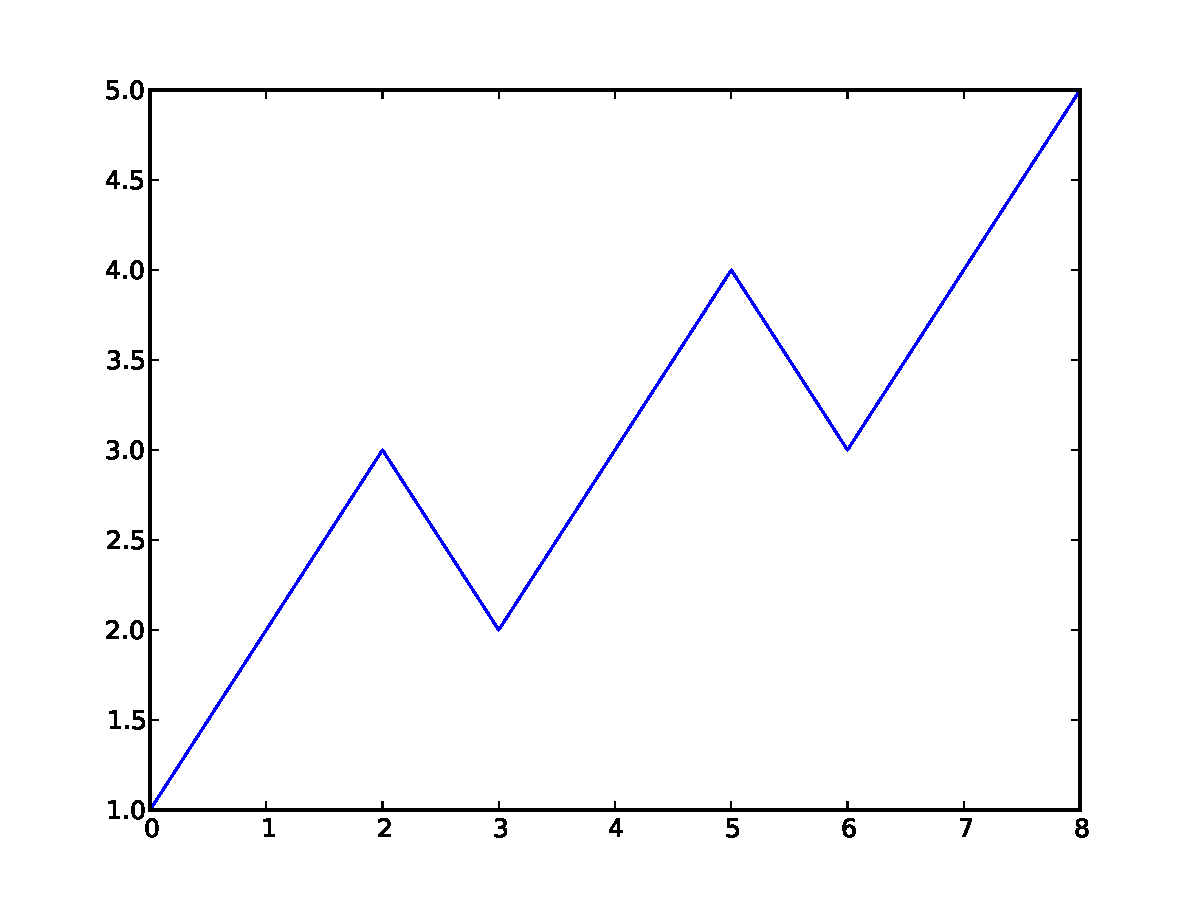
\includegraphics{zigzagPlotDemo.pdf}}
\caption{Interactive plot window}\label{chap5/chap5_plot:fig-zigzagplotdemo}\end{figure}

A window should appear with a plot that looks something like the {\hyperref[chap5/chap5_plot:fig-zigzagplotdemo]{\emph{Interactive plot window}}} shown here.  By default, the \code{plot} function draws a line between the data points that were entered.  You can save this plot to an image file by clicking on the floppy disk icon at the top of the plot window.  You can also zoom, pan, scroll through the plot, and return to the original view using the other icons in the plot window.  Experimenting with them reveals their functions.

When you are finished, be sure to close the plot window.

Let's take a closer look at the \code{plot} function.  It is used to plot \(x\)-\(y\) data sets and is written like this

\begin{Verbatim}[commandchars=\\\{\}]
\PYG{n}{plot}\PYG{p}{(}\PYG{n}{x}\PYG{p}{,} \PYG{n}{y}\PYG{p}{)}
\end{Verbatim}

where \code{x} and \code{y} are arrays (or lists) that have the same size.  If the \code{x} array is missing, that is, if there is only a single array, as in our example above, the \code{plot} function uses \code{0, 1, ..., N-1} for the \code{x} array, where \code{N} is the size of the \code{y} array.  Thus, the \code{plot} function provides a quick graphical way of examining a data set.

More typically, you supply both an \(x\) and a \(y\) data set to plot.  Taking things a bit further, you may also want to plot several data sets on the same graph, use symbols as well as lines, label the axes, create a title and a legend, and control the color of symbols and lines.  All of this is possible but requires calling a number of plotting functions.  For this reason, plotting is usually done using a Python script or program.


\section{Basic plotting}
\label{chap5/chap5_plot:chap5basicplotting}\label{chap5/chap5_plot:basic-plotting}
\index{plots!basic}
The quickest way to learn how to plot using the MatPlotLib library is by example.  For our first task, let's plot the sine function over the interval from 0 to \(4\pi\).  The main plotting function \code{plot} in MatPlotLib does not plot functions \emph{per se}, it plots \((x,y)\) data points.  As we shall see, we can instruct the function \code{plot} either to just draw point---or dots---at each data point, or we can instruct it to draw straight lines between the data points.  To create the illusion of the smooth function that the sine function is, we need to create enough \((x,y)\) data points so that when \code{plot} draws straight lines between the data points, the function appears to be smooth.  The sine function undergoes two full oscillations with two maxima and two minima between 0 and \(4\pi\).  So let's start by creating an array with 33 data points between 0 and \(4\pi\), and then let MatPlotLib draw a straight line between them.  Our code consists of four parts
\begin{itemize}
\item {} 
import the NumPy and MatPlotLib modules (lines 1-2 below)

\item {} 
create the \((x,y)\) data arrays (lines 3-4 below)

\item {} 
have \code{plot} draw straight lines between the \((x,y)\) data points (line 5 below)

\item {} 
display the plot in a figure window using the \code{show} function (line 6 below)

\end{itemize}

Here is our code, which consists of only 6 lines:

\begin{Verbatim}[commandchars=\\\{\},numbers=left,firstnumber=1,stepnumber=1]
\PYG{k+kn}{import} \PYG{n+nn}{numpy} \PYG{k+kn}{as} \PYG{n+nn}{np}
\PYG{k+kn}{import} \PYG{n+nn}{matplotlib.pyplot} \PYG{k+kn}{as} \PYG{n+nn}{plt}
\PYG{n}{x} \PYG{o}{=} \PYG{n}{np}\PYG{o}{.}\PYG{n}{linspace}\PYG{p}{(}\PYG{l+m+mi}{0}\PYG{p}{,} \PYG{l+m+mf}{4.}\PYG{o}{*}\PYG{n}{np}\PYG{o}{.}\PYG{n}{pi}\PYG{p}{,} \PYG{l+m+mi}{33}\PYG{p}{)}
\PYG{n}{y} \PYG{o}{=} \PYG{n}{np}\PYG{o}{.}\PYG{n}{sin}\PYG{p}{(}\PYG{n}{x}\PYG{p}{)}
\PYG{n}{plt}\PYG{o}{.}\PYG{n}{plot}\PYG{p}{(}\PYG{n}{x}\PYG{p}{,} \PYG{n}{y}\PYG{p}{)}
\PYG{n}{plt}\PYG{o}{.}\PYG{n}{show}\PYG{p}{(}\PYG{p}{)}
\end{Verbatim}
\begin{figure}[htbp]
\centering
\capstart

\scalebox{0.700000}{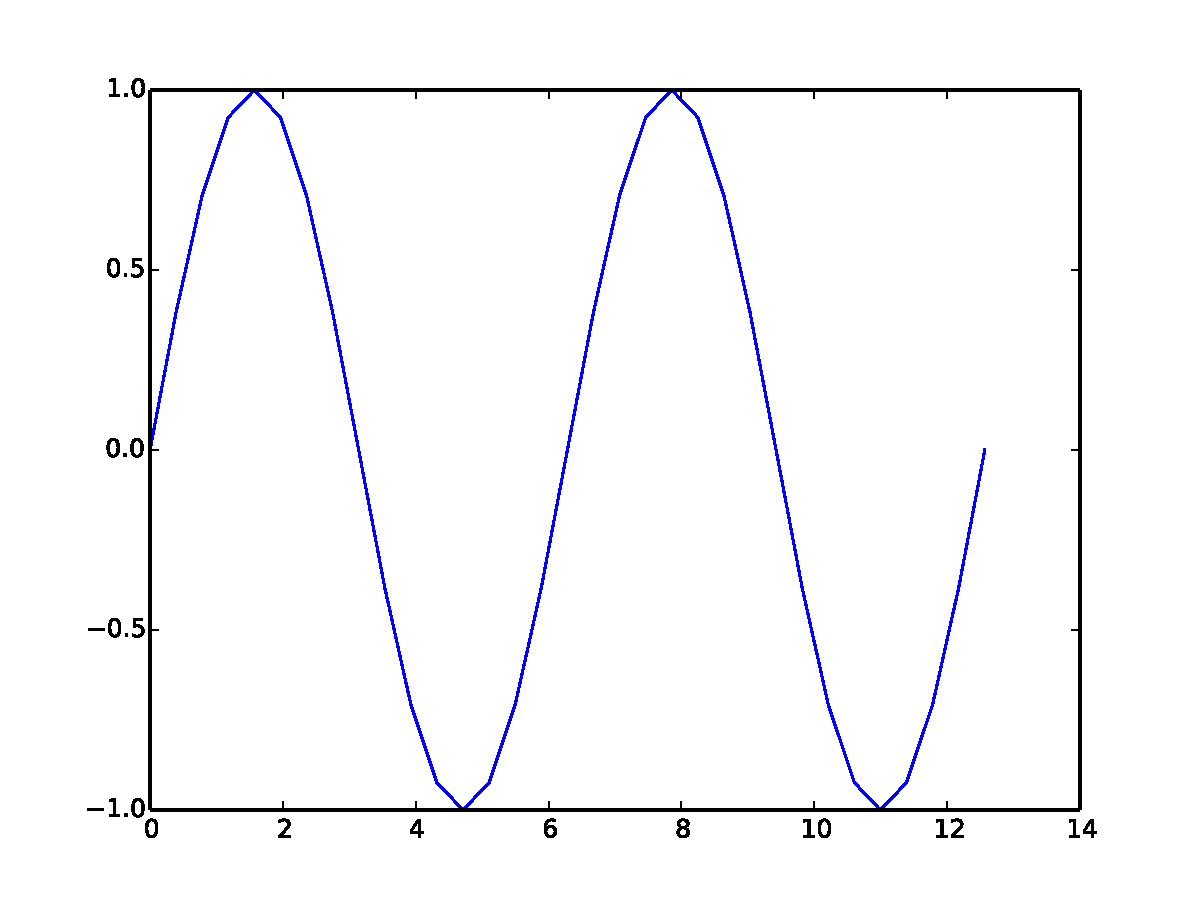
\includegraphics{sinePlot.pdf}}
\caption{Sine function}\label{chap5/chap5_plot:fig-sineplot}\end{figure}

Only 6 lines suffice to create the plot, which consists of the sine function over the interval from 0 to \(4\pi\), as advertised, as well as axes annotated with nice whole numbers over the appropriate interval.  It's a pretty nice plot made with very little code.

One problem, however, is that while the plot oscillates like a sine wave, it is not smooth.  This is because we did not create the \((x,y)\) arrays with enough data points.  To correct this, we need more data points.  The plot below was created using the same program shown above but with 129 \((x,y)\) data points instead of 33.  Try it out your self by copying the above program and replacing 33 in line 3 with 129 so that the function \code{linspace} creates an array with 129 data points instead of 33.
\begin{figure}[htbp]
\centering
\capstart

\scalebox{0.700000}{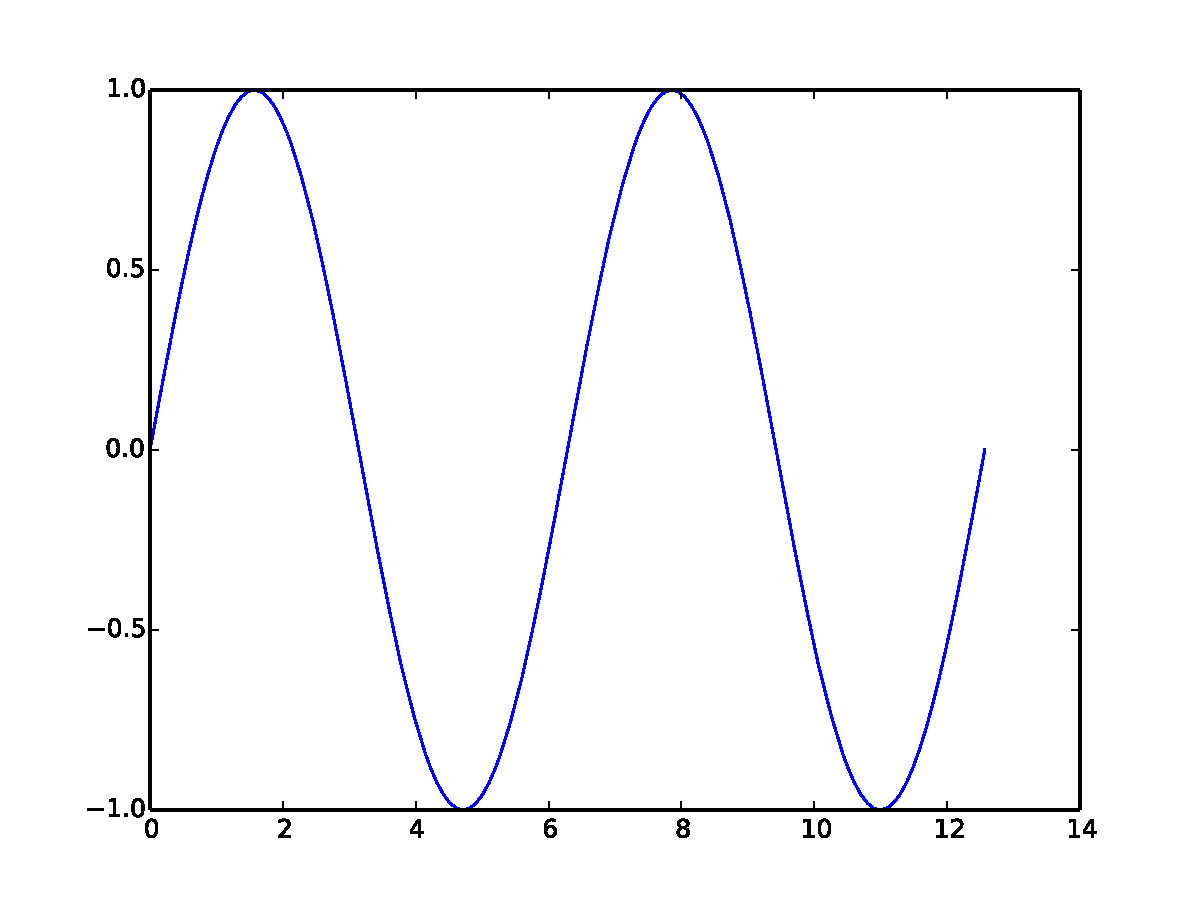
\includegraphics{sinePlotDenserXY.pdf}}
\caption{Sine function plotted using more data points}\label{chap5/chap5_plot:fig-sineplotdenserxy}\end{figure}

The code above illustrates how plots can be made with very little code using the MatPlotLib module.  In making this plot, MatPlotLib has made a number of choices, such as the size of the figure, the blue color of the line, even the fact that by default a line is drawn between successive data points in the \((x,y)\) arrays.  All of these choices can be changed by explicitly instructing MatPlotLib to do so.  This involves including more arguments in the function calls we have used and using new functions that control other properties of the plot.  The next example illustrates a few of the simpler embellishments that are possible.

In the {\hyperref[chap5/chap5_plot:fig-wavypulse]{\emph{Wavy pulse}}} figure, we plot two \((x,y)\) data sets: a smooth line curve and some data represented by red circles.  In this plot, we label the \(x\) and \(y\) axes, create a legend, and draw lines to indicate where \(x\) and \(y\) are zero.  The code that creates this plot is shown below.

\begin{Verbatim}[commandchars=\\\{\},numbers=left,firstnumber=1,stepnumber=1]
\PYG{k+kn}{import} \PYG{n+nn}{numpy} \PYG{k+kn}{as} \PYG{n+nn}{np}
\PYG{k+kn}{import} \PYG{n+nn}{matplotlib.pyplot} \PYG{k+kn}{as} \PYG{n+nn}{plt}

\PYG{c}{\PYGZsh{} read data from file}
\PYG{n}{xdata}\PYG{p}{,} \PYG{n}{ydata} \PYG{o}{=} \PYG{n}{np}\PYG{o}{.}\PYG{n}{loadtxt}\PYG{p}{(}\PYG{l+s}{\PYGZsq{}}\PYG{l+s}{wavePulseData.txt}\PYG{l+s}{\PYGZsq{}}\PYG{p}{,} \PYG{n}{unpack}\PYG{o}{=}\PYG{n+nb+bp}{True}\PYG{p}{)}

\PYG{c}{\PYGZsh{} create x and y arrays for theory}
\PYG{n}{x} \PYG{o}{=} \PYG{n}{np}\PYG{o}{.}\PYG{n}{linspace}\PYG{p}{(}\PYG{o}{\PYGZhy{}}\PYG{l+m+mf}{10.}\PYG{p}{,} \PYG{l+m+mf}{10.}\PYG{p}{,} \PYG{l+m+mi}{200}\PYG{p}{)}
\PYG{n}{y} \PYG{o}{=} \PYG{n}{np}\PYG{o}{.}\PYG{n}{sin}\PYG{p}{(}\PYG{n}{x}\PYG{p}{)} \PYG{o}{*} \PYG{n}{np}\PYG{o}{.}\PYG{n}{exp}\PYG{p}{(}\PYG{o}{\PYGZhy{}}\PYG{p}{(}\PYG{n}{x}\PYG{o}{/}\PYG{l+m+mf}{5.0}\PYG{p}{)}\PYG{o}{*}\PYG{o}{*}\PYG{l+m+mi}{2}\PYG{p}{)}

\PYG{c}{\PYGZsh{} create plot}
\PYG{n}{plt}\PYG{o}{.}\PYG{n}{figure}\PYG{p}{(}\PYG{l+m+mi}{1}\PYG{p}{,} \PYG{n}{figsize} \PYG{o}{=} \PYG{p}{(}\PYG{l+m+mi}{6}\PYG{p}{,}\PYG{l+m+mi}{4}\PYG{p}{)} \PYG{p}{)}
\PYG{n}{plt}\PYG{o}{.}\PYG{n}{plot}\PYG{p}{(}\PYG{n}{x}\PYG{p}{,} \PYG{n}{y}\PYG{p}{,} \PYG{l+s}{\PYGZsq{}}\PYG{l+s}{b\PYGZhy{}}\PYG{l+s}{\PYGZsq{}}\PYG{p}{,} \PYG{n}{label}\PYG{o}{=}\PYG{l+s}{\PYGZsq{}}\PYG{l+s}{theory}\PYG{l+s}{\PYGZsq{}}\PYG{p}{)}
\PYG{n}{plt}\PYG{o}{.}\PYG{n}{plot}\PYG{p}{(}\PYG{n}{xdata}\PYG{p}{,} \PYG{n}{ydata}\PYG{p}{,} \PYG{l+s}{\PYGZsq{}}\PYG{l+s}{ro}\PYG{l+s}{\PYGZsq{}}\PYG{p}{,} \PYG{n}{label}\PYG{o}{=}\PYG{l+s}{\PYGZdq{}}\PYG{l+s}{data}\PYG{l+s}{\PYGZdq{}}\PYG{p}{)}
\PYG{n}{plt}\PYG{o}{.}\PYG{n}{xlabel}\PYG{p}{(}\PYG{l+s}{\PYGZsq{}}\PYG{l+s}{x}\PYG{l+s}{\PYGZsq{}}\PYG{p}{)}
\PYG{n}{plt}\PYG{o}{.}\PYG{n}{ylabel}\PYG{p}{(}\PYG{l+s}{\PYGZsq{}}\PYG{l+s}{transverse displacement}\PYG{l+s}{\PYGZsq{}}\PYG{p}{)}
\PYG{n}{plt}\PYG{o}{.}\PYG{n}{legend}\PYG{p}{(}\PYG{n}{loc}\PYG{o}{=}\PYG{l+s}{\PYGZsq{}}\PYG{l+s}{upper right}\PYG{l+s}{\PYGZsq{}}\PYG{p}{)}
\PYG{n}{plt}\PYG{o}{.}\PYG{n}{axhline}\PYG{p}{(}\PYG{n}{color} \PYG{o}{=} \PYG{l+s}{\PYGZsq{}}\PYG{l+s}{gray}\PYG{l+s}{\PYGZsq{}}\PYG{p}{,} \PYG{n}{zorder}\PYG{o}{=}\PYG{o}{\PYGZhy{}}\PYG{l+m+mi}{1}\PYG{p}{)}
\PYG{n}{plt}\PYG{o}{.}\PYG{n}{axvline}\PYG{p}{(}\PYG{n}{color} \PYG{o}{=} \PYG{l+s}{\PYGZsq{}}\PYG{l+s}{gray}\PYG{l+s}{\PYGZsq{}}\PYG{p}{,} \PYG{n}{zorder}\PYG{o}{=}\PYG{o}{\PYGZhy{}}\PYG{l+m+mi}{1}\PYG{p}{)}

\PYG{c}{\PYGZsh{} save plot to file}
\PYG{n}{plt}\PYG{o}{.}\PYG{n}{savefig}\PYG{p}{(}\PYG{l+s}{\PYGZsq{}}\PYG{l+s}{WavyPulse.pdf}\PYG{l+s}{\PYGZsq{}}\PYG{p}{)}

\PYG{c}{\PYGZsh{} display plot on screen}
\PYG{n}{plt}\PYG{o}{.}\PYG{n}{show}\PYG{p}{(}\PYG{p}{)}
\end{Verbatim}
\begin{figure}[htbp]
\centering
\capstart

\scalebox{0.800000}{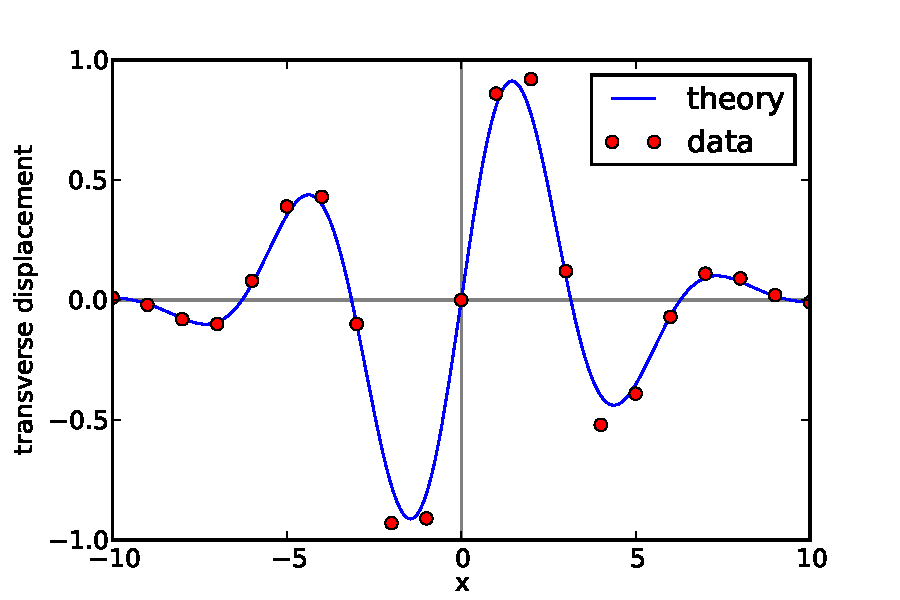
\includegraphics{WavyPulse.pdf}}
\caption{Wavy pulse}\label{chap5/chap5_plot:fig-wavypulse}\end{figure}

If you have read the first four chapters, the code in lines 1-9 in the above script should  be familiar to you.  Fist, the script loads the NumPy and MatPlotLib modules, then reads data from a data file into two arrays, \code{xdata} and \code{ydata}, and then creates two more arrays, \code{x} and \code{y}.  The first pair or arrays, \code{xdata} and \code{ydata}, contain the \(x\)-\(y\) data that are plotted as red circles in the {\hyperref[chap5/chap5_plot:fig-wavypulse]{\emph{Wavy pulse}}} figure; the arrays created in line 8 and 9 contain the \(x\)-\(y\) data that are plotted as a blue line.

The functions that do the plotting begin on line 12.  Let's go through them one by one and see what they do.  You will notice in several cases that \emph{keyword arguments} (\code{kwargs}) are used in several cases.  Keyword arguments are \emph{optional} arguments that have the form \code{kwarg=} \emph{data}, where \emph{data} might be a number, a string, a tuple, or some other form of data.
\begin{quote}
\begin{description}
\item[{\code{figure()}}] \leavevmode
creates a blank figure window.  If it has no arguments, it creates a window that is 8 inches wide and 6 inches high by default, although the size that appears on your computer depends on your screen's resolution.  For most computers, it will be much smaller.  You can create a window whose size differs from the default using the optional keyword argument \code{figsize}, as we have done here.  If you use \code{figsize}, set it equal to a 2-element tuple where the elements are the width and height, respectively, of the plot.  Multiple calls to \code{figure()} opens multiple windows:  \code{figure(1)} opens up one window for plotting, \code{figure(2)} another, and \code{figure(3)} yet another.

\item[{\code{plot(x, y,} \emph{optional arguments} \code{)}}] \leavevmode
graphs the \(x\)-\(y\) data in the arrays \code{x} and \code{y}.  The third argument is a format string that specifies the color and the type of line or symbol that is used to plot the data.  The string \code{'ro'} specifies a red (\code{r}) circle (\code{o}).  The string \code{'b-'} specifies a blue (\code{b}) solid line (\code{-}).  The keyword argument \code{label} is set equal to a string that labels the data if the \code{legend} function is called subsequently.

\item[{\code{xlabel(} \emph{string} \code{)}}] \leavevmode
takes a string argument that specifies the label for the graph's \(x\)-axis.

\item[{\code{ylabel(} \emph{string} \code{)}}] \leavevmode
takes a string argument that specifies the label for the graph's \(y\)-axis.

\item[{\code{legend()}}] \leavevmode
makes a legend for the data plotted.  Each \(x\)-\(y\) data set is labeled  using the string that was supplied by the \code{label} keyword in the \code{plot} function that graphed the data set.  The \code{loc} keyword argument specifies the location of the legend.

\item[{\code{axhline()}}] \leavevmode
draws a horizontal line across the width of the plot at \code{y=0}.  The optional keyword argument \code{color} is a string that specifies the color of the line.  The default color is black.  The optional keyword argument \code{zorder} is an integer that specifies which plotting elements are in front of or behind others.  By default, new plotting elements appear \emph{on top of} previously plotted elements and have a value of \code{zorder=0}.  By specifying \code{zorder=-1}, the horizontal line is plotted \emph{behind} all existing plot elements that have not be assigned an explicit \code{zorder} less than -1.

\item[{\code{axvline()}}] \leavevmode
draws a vertical line from the top to the bottom of the plot at \code{x=0}.  See \code{axhline()} for explanation of the arguments.

\item[{\code{savefig(} \emph{string} \code{)}}] \leavevmode
saves the figure to data data file with a name specified by the string argument.  The string argument can also contain path information if you want to save the file so some place other than the default directory.

\item[{\code{show()}}] \leavevmode
displays the plot on the computer screen.  No screen output is produced before this function is called.

\end{description}
\end{quote}

\index{MatPlotLib functions!figure}\index{MatPlotLib functions!plot}\index{MatPlotLib functions!xlabel, ylabel}\index{MatPlotLib functions!legend}\index{MatPlotLib functions!ayhline, axhline}\index{MatPlotLib functions!savefig}\index{MatPlotLib functions!show}
To plot the solid blue line, the code uses the \code{'b-'} format specifier in the \code{plot} function call.  It is important to understand that MatPlotLib draws \emph{straight lines} between data points.  Therefore, the curve will appear smooth only if the data in the NumPy arrays are sufficiently dense.  If the space between data points is too large, the straight lines the \code{plot} function draws between data points will be visible.  For plotting a typical function, something on the order of 100-200 data points usually produces a smooth curve, depending on just how curvy the function is.  On the other hand, only two points are required to draw a smooth straight line.

Detailed information about the MatPlotLib plotting functions are available online, starting with the site \href{http://matplotlib.org/api/pyplot\_summary.html}{http://matplotlib.org/api/pyplot\_summary.html}.  The main MatPlotLib site is \href{http://matplotlib.org/}{http://matplotlib.org/}.


\subsection{Specifying line and symbol types and colors}
\label{chap5/chap5_plot:specifying-line-and-symbol-types-and-colors}
In the above example, we illustrated how to draw one line type (solid), one symbol type (circle), and two colors (blue and red).  There are many more possibilities, which are specified in the tables below.  The way it works is to specify a string consisting of one or more plotting format specifiers.  There are two types of format specifiers, one for the line or symbol type and another for the color.  It does not matter in which order the  format specifiers are listed in the string.  Examples are given following the two tables.  Try them out to make sure you understand how these plotting format specifiers work.

\index{plots!line and symbol specifiers}
The first table below shows the characters used to specify the line or symbol type that is used.  If a line type is chosen, the lines are drawn between the data points.  If a marker type is chosen, the a marker is plotted at each data point.
\begin{quote}

\begin{tabulary}{\linewidth}{|L|L|L|L|}
\hline
\textsf{\relax 
character
} & \textsf{\relax 
description
} & \textsf{\relax 
character
} & \textsf{\relax 
description
}\\
\hline
\code{-}
 & 
solid line style
 & 
\code{3}
 & 
tri\_left marker
\\

\code{-{-}}
 & 
dashed line style
 & 
\code{4}
 & 
tri\_right marker
\\

\code{-.}
 & 
dash-dot line style
 & 
\code{s}
 & 
square marker
\\

\code{:}
 & 
dotted line style
 & 
\code{p}
 & 
pentagon marker
\\

\code{.}
 & 
point marker
 & 
\code{*}
 & 
star marker
\\

\code{,}
 & 
pixel marker
 & 
\code{h}
 & 
hexagon1 marker
\\

\code{o}
 & 
circle marker
 & 
\code{H}
 & 
hexagon2 marker
\\

\code{v}
 & 
triangle\_down marker
 & 
\code{+}
 & 
plus marker
\\

\code{\textasciicircum{}}
 & 
triangle\_up marker
 & 
\code{x}
 & 
x marker
\\

\code{\textless{}}
 & 
triangle\_left marker
 & 
\code{D}
 & 
diamond marker
\\

\code{\textgreater{}}
 & 
triangle\_right marker
 & 
\code{d}
 & 
thin\_diamond marker
\\

\code{1}
 & 
tri\_down marker
 & 
\code{\textbar{}}
 & 
vline marker
\\

\code{2}
 & 
tri\_up marker
 & 
\code{\_}
 & 
hline marker
\\
\hline\end{tabulary}

\end{quote}

This second table gives the character codes for eight different colors.  Many more are possible but the color specification becomes more complex. You can consult the web-based MatPlotLib documentation for further details.
\begin{quote}

\begin{tabulary}{\linewidth}{|L|L|}
\hline
\textsf{\relax 
character
} & \textsf{\relax 
color
}\\
\hline
\code{b}
 & 
blue
\\

\code{g}
 & 
green
\\

\code{r}
 & 
red
\\

\code{c}
 & 
cyan
\\

\code{m}
 & 
magenta
\\

\code{y}
 & 
yellow
\\

\code{k}
 & 
black
\\

\code{w}
 & 
white
\\
\hline\end{tabulary}

\end{quote}

Here are some examples of how these format specifiers can be used:

\begin{Verbatim}[commandchars=\\\{\}]
\PYG{n}{plot}\PYG{p}{(}\PYG{n}{x}\PYG{p}{,} \PYG{n}{y}\PYG{p}{,} \PYG{l+s}{\PYGZsq{}}\PYG{l+s}{ro}\PYG{l+s}{\PYGZsq{}}\PYG{p}{)}    \PYG{c}{\PYGZsh{} plots red circles}
\PYG{n}{plot}\PYG{p}{(}\PYG{n}{x}\PYG{p}{,} \PYG{n}{y}\PYG{p}{,} \PYG{l+s}{\PYGZsq{}}\PYG{l+s}{ks\PYGZhy{}}\PYG{l+s}{\PYGZsq{}}\PYG{p}{)}   \PYG{c}{\PYGZsh{} plot black squares connected by black lines}
\PYG{n}{plot}\PYG{p}{(}\PYG{n}{x}\PYG{p}{,} \PYG{n}{y}\PYG{p}{,} \PYG{l+s}{\PYGZsq{}}\PYG{l+s}{g\PYGZca{}}\PYG{l+s}{\PYGZsq{}}\PYG{p}{)}    \PYG{c}{\PYGZsh{} plots green triangles that point up}

\PYG{n}{plot}\PYG{p}{(}\PYG{n}{x}\PYG{p}{,} \PYG{n}{y}\PYG{p}{,} \PYG{l+s}{\PYGZsq{}}\PYG{l+s}{k\PYGZhy{}}\PYG{l+s}{\PYGZsq{}}\PYG{p}{)}    \PYG{c}{\PYGZsh{} plots a black line between the points}
\PYG{n}{plot}\PYG{p}{(}\PYG{n}{x}\PYG{p}{,} \PYG{n}{y}\PYG{p}{,} \PYG{l+s}{\PYGZsq{}}\PYG{l+s}{ms}\PYG{l+s}{\PYGZsq{}}\PYG{p}{)}    \PYG{c}{\PYGZsh{} plots magenta squares}
\end{Verbatim}

You can also make two calls sequentially for added versatility.  For example, by sequentially calling the last two plot calls, the plot produces magenta squares on top of black lines connecting the data points.

These format specifiers give rudimentary control of the plotting symbols and lines.  MatPlotLib provides much more precise and detailed control of the plotting symbol size, line types, and colors using optional keyword arguments instead of the plotting format strings introduced above.  For example, the following command creates a plot of large yellow diamond symbols with blue edges connected by a green dashed line:

\begin{Verbatim}[commandchars=\\\{\}]
\PYG{n}{plot}\PYG{p}{(}\PYG{n}{x}\PYG{p}{,} \PYG{n}{y}\PYG{p}{,} \PYG{n}{color}\PYG{o}{=}\PYG{l+s}{\PYGZsq{}}\PYG{l+s}{green}\PYG{l+s}{\PYGZsq{}}\PYG{p}{,} \PYG{n}{linestyle}\PYG{o}{=}\PYG{l+s}{\PYGZsq{}}\PYG{l+s}{dashed}\PYG{l+s}{\PYGZsq{}}\PYG{p}{,} \PYG{n}{marker}\PYG{o}{=}\PYG{l+s}{\PYGZsq{}}\PYG{l+s}{d}\PYG{l+s}{\PYGZsq{}}\PYG{p}{,}
     \PYG{n}{markerfacecolor}\PYG{o}{=}\PYG{l+s}{\PYGZsq{}}\PYG{l+s}{yellow}\PYG{l+s}{\PYGZsq{}}\PYG{p}{,} \PYG{n}{markersize}\PYG{o}{=}\PYG{l+m+mi}{12}\PYG{p}{,}
     \PYG{n}{markeredgecolor}\PYG{o}{=}\PYG{l+s}{\PYGZsq{}}\PYG{l+s}{blue}\PYG{l+s}{\PYGZsq{}}\PYG{p}{)}
\end{Verbatim}

Try it out!  The online MatPlotLib documentation provides all the plotting format keyword arguments and their possible values.


\subsection{Error bars}
\label{chap5/chap5_plot:error-bars}
\index{plots!error bars}
When plotting experimental data it is customary to include error bars that indicate graphically the degree of uncertainty that exists in the measurement of each data point.  The MatPlotLib function \code{errorbar} plots data with error bars attached.  It can be used in a way that either replaces or augments the \code{plot} function.  Both vertical and horizontal error bars can be displayed.  The figure below illustrates the use of error bars.
\begin{figure}[htbp]
\centering
\capstart

\scalebox{0.750000}{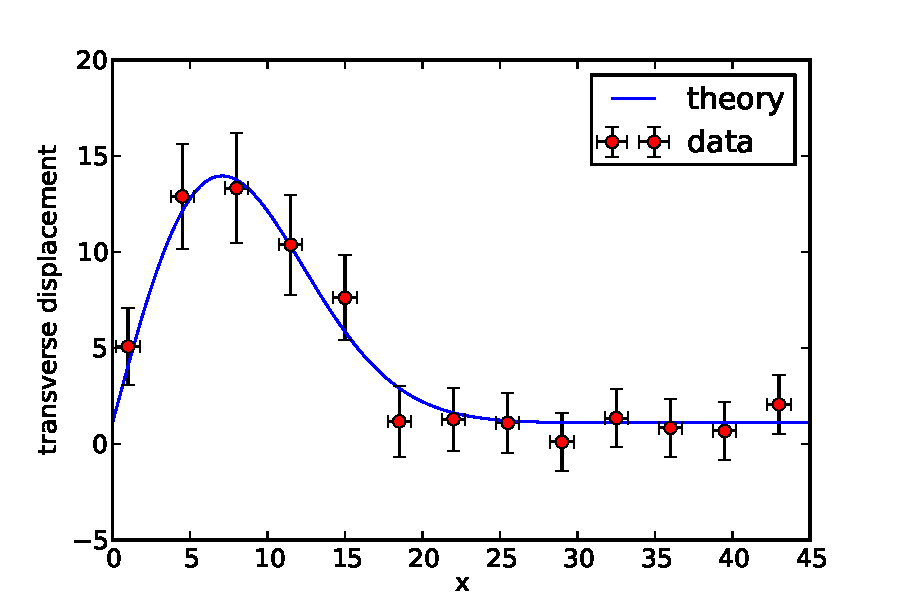
\includegraphics{ExpDecay.pdf}}
\caption{Error Bars}\label{chap5/chap5_plot:fig-expdecay}\end{figure}

When error bars are desired, you typically replace the \code{plot} function with the \code{errorbar} function.  The first two arguments of the  \code{errorbar} function are the \code{x} and \code{y} arrays to be plotted, just as for the \code{plot} function.  The keyword \code{fmt} \emph{must be used} to specify the format of the points to be plotted; the format specifiers are the same as for \code{plot}.  The keywords \code{xerr} and \code{yerr} are used to specify the \(x\) and \(y\) error bars.  Setting one or both of them to a constant specifies one size for all the error bars.  Alternatively, setting one or both of them equal to an array that has the same length as the \code{x} and \code{y} arrays allows you to give each data point an error bar with a different value.  If you only want \(y\) error bars, then you should only specify the \code{yerr} keyword and omit the \code{xerr} keyword.  The color of the error bars is set with the keyword \code{ecolor}.

The code and plot below illustrates how to make error bars and was used to make the above plot.  Lines 14 and 15 contain the call to the \code{errorbar} function.  The \(x\) error bars are all set to a constant value of 0.75, meaning that the error bars extend 0.75 to the left and 0.75 to the right of each data point.  The \(y\) error bars are set equal to an array, which was read in from the data file containing the data to be plotted, so each data point has a different \(y\) error bar.  By the way, leaving out the \code{xerr} keyword argument in the \code{errorbar} function call below would mean that only the \(y\) error bars would be plotted.

\begin{Verbatim}[commandchars=\\\{\},numbers=left,firstnumber=1,stepnumber=1]
\PYG{k+kn}{import} \PYG{n+nn}{numpy} \PYG{k+kn}{as} \PYG{n+nn}{np}
\PYG{k+kn}{import} \PYG{n+nn}{matplotlib.pyplot} \PYG{k+kn}{as} \PYG{n+nn}{plt}

\PYG{c}{\PYGZsh{} read data from file}
\PYG{n}{xdata}\PYG{p}{,} \PYG{n}{ydata}\PYG{p}{,} \PYG{n}{yerror} \PYG{o}{=} \PYG{n}{np}\PYG{o}{.}\PYG{n}{loadtxt}\PYG{p}{(}\PYG{l+s}{\PYGZsq{}}\PYG{l+s}{expDecayData.txt}\PYG{l+s}{\PYGZsq{}}\PYG{p}{,} \PYG{n}{unpack}\PYG{o}{=}\PYG{n+nb+bp}{True}\PYG{p}{)}

\PYG{c}{\PYGZsh{} create theoretical fitting curve}
\PYG{n}{x} \PYG{o}{=} \PYG{n}{np}\PYG{o}{.}\PYG{n}{linspace}\PYG{p}{(}\PYG{l+m+mi}{0}\PYG{p}{,} \PYG{l+m+mi}{45}\PYG{p}{,} \PYG{l+m+mi}{128}\PYG{p}{)}
\PYG{n}{y} \PYG{o}{=} \PYG{l+m+mf}{1.1}\PYG{o}{+} \PYG{l+m+mf}{3.0}\PYG{o}{*}\PYG{n}{x}\PYG{o}{*}\PYG{n}{np}\PYG{o}{.}\PYG{n}{exp}\PYG{p}{(}\PYG{o}{\PYGZhy{}}\PYG{p}{(}\PYG{n}{x}\PYG{o}{/}\PYG{l+m+mf}{10.0}\PYG{p}{)}\PYG{o}{*}\PYG{o}{*}\PYG{l+m+mi}{2}\PYG{p}{)}

\PYG{c}{\PYGZsh{} create plot}
\PYG{n}{plt}\PYG{o}{.}\PYG{n}{figure}\PYG{p}{(}\PYG{l+m+mi}{1}\PYG{p}{,} \PYG{n}{figsize} \PYG{o}{=} \PYG{p}{(}\PYG{l+m+mi}{6}\PYG{p}{,}\PYG{l+m+mi}{4}\PYG{p}{)} \PYG{p}{)}
\PYG{n}{plt}\PYG{o}{.}\PYG{n}{plot}\PYG{p}{(}\PYG{n}{x}\PYG{p}{,} \PYG{n}{y}\PYG{p}{,} \PYG{l+s}{\PYGZsq{}}\PYG{l+s}{b\PYGZhy{}}\PYG{l+s}{\PYGZsq{}}\PYG{p}{,} \PYG{n}{label}\PYG{o}{=}\PYG{l+s}{\PYGZdq{}}\PYG{l+s}{theory}\PYG{l+s}{\PYGZdq{}}\PYG{p}{)}
\PYG{n}{plt}\PYG{o}{.}\PYG{n}{errorbar}\PYG{p}{(}\PYG{n}{xdata}\PYG{p}{,} \PYG{n}{ydata}\PYG{p}{,} \PYG{n}{fmt}\PYG{o}{=}\PYG{l+s}{\PYGZsq{}}\PYG{l+s}{ro}\PYG{l+s}{\PYGZsq{}}\PYG{p}{,} \PYG{n}{label}\PYG{o}{=}\PYG{l+s}{\PYGZdq{}}\PYG{l+s}{data}\PYG{l+s}{\PYGZdq{}}\PYG{p}{,}
             \PYG{n}{xerr}\PYG{o}{=}\PYG{l+m+mf}{0.75}\PYG{p}{,} \PYG{n}{yerr}\PYG{o}{=}\PYG{n}{yerror}\PYG{p}{,} \PYG{n}{ecolor}\PYG{o}{=}\PYG{l+s}{\PYGZsq{}}\PYG{l+s}{black}\PYG{l+s}{\PYGZsq{}}\PYG{p}{)}
\PYG{n}{plt}\PYG{o}{.}\PYG{n}{xlabel}\PYG{p}{(}\PYG{l+s}{\PYGZsq{}}\PYG{l+s}{x}\PYG{l+s}{\PYGZsq{}}\PYG{p}{)}
\PYG{n}{plt}\PYG{o}{.}\PYG{n}{ylabel}\PYG{p}{(}\PYG{l+s}{\PYGZsq{}}\PYG{l+s}{transverse displacement}\PYG{l+s}{\PYGZsq{}}\PYG{p}{)}
\PYG{n}{plt}\PYG{o}{.}\PYG{n}{legend}\PYG{p}{(}\PYG{n}{loc}\PYG{o}{=}\PYG{l+s}{\PYGZsq{}}\PYG{l+s}{upper right}\PYG{l+s}{\PYGZsq{}}\PYG{p}{)}

\PYG{c}{\PYGZsh{} save plot to file}
\PYG{n}{plt}\PYG{o}{.}\PYG{n}{savefig}\PYG{p}{(}\PYG{l+s}{\PYGZsq{}}\PYG{l+s}{ExpDecay.pdf}\PYG{l+s}{\PYGZsq{}}\PYG{p}{)}

\PYG{c}{\PYGZsh{} display plot on screen}
\PYG{n}{plt}\PYG{o}{.}\PYG{n}{show}\PYG{p}{(}\PYG{p}{)}
\end{Verbatim}

We have more to say about the \code{errorbar} function in the sections on  logarithmic plots.  But the brief introduction given here should suffice for making most plots not involving logarithmic axes.


\subsection{Setting plotting limits and excluding data}
\label{chap5/chap5_plot:setting-plotting-limits-and-excluding-data}
It turns out that you often want to restrict the range of numerical values over which you plot data or functions.  In these cases you may need to manually specify the plotting window or, alternatively, you may wish to exclude data points that are outside some set of limits.  Here we demonstrate methods for doing this.


\subsubsection{Setting plotting limits}
\label{chap5/chap5_plot:setting-plotting-limits}
\index{plots!setting axis limits}
Suppose you want to plot the tangent function over the interval from 0 to 10.  The following script offers an straightforward first attempt.

\begin{Verbatim}[commandchars=\\\{\}]
\PYG{k+kn}{import} \PYG{n+nn}{numpy} \PYG{k+kn}{as} \PYG{n+nn}{np}
\PYG{k+kn}{import} \PYG{n+nn}{matplotlib.pyplot} \PYG{k+kn}{as} \PYG{n+nn}{plt}

\PYG{n}{theta} \PYG{o}{=} \PYG{n}{np}\PYG{o}{.}\PYG{n}{arange}\PYG{p}{(}\PYG{l+m+mf}{0.01}\PYG{p}{,} \PYG{l+m+mf}{10.}\PYG{p}{,} \PYG{l+m+mf}{0.04}\PYG{p}{)}
\PYG{n}{ytan} \PYG{o}{=} \PYG{n}{np}\PYG{o}{.}\PYG{n}{tan}\PYG{p}{(}\PYG{n}{theta}\PYG{p}{)}

\PYG{n}{plt}\PYG{o}{.}\PYG{n}{figure}\PYG{p}{(}\PYG{p}{)}
\PYG{n}{plt}\PYG{o}{.}\PYG{n}{plot}\PYG{p}{(}\PYG{n}{theta}\PYG{p}{,} \PYG{n}{ytan}\PYG{p}{)}
\PYG{n}{plt}\PYG{o}{.}\PYG{n}{show}\PYG{p}{(}\PYG{p}{)}
\end{Verbatim}
\begin{figure}[htbp]
\centering

\scalebox{0.800000}{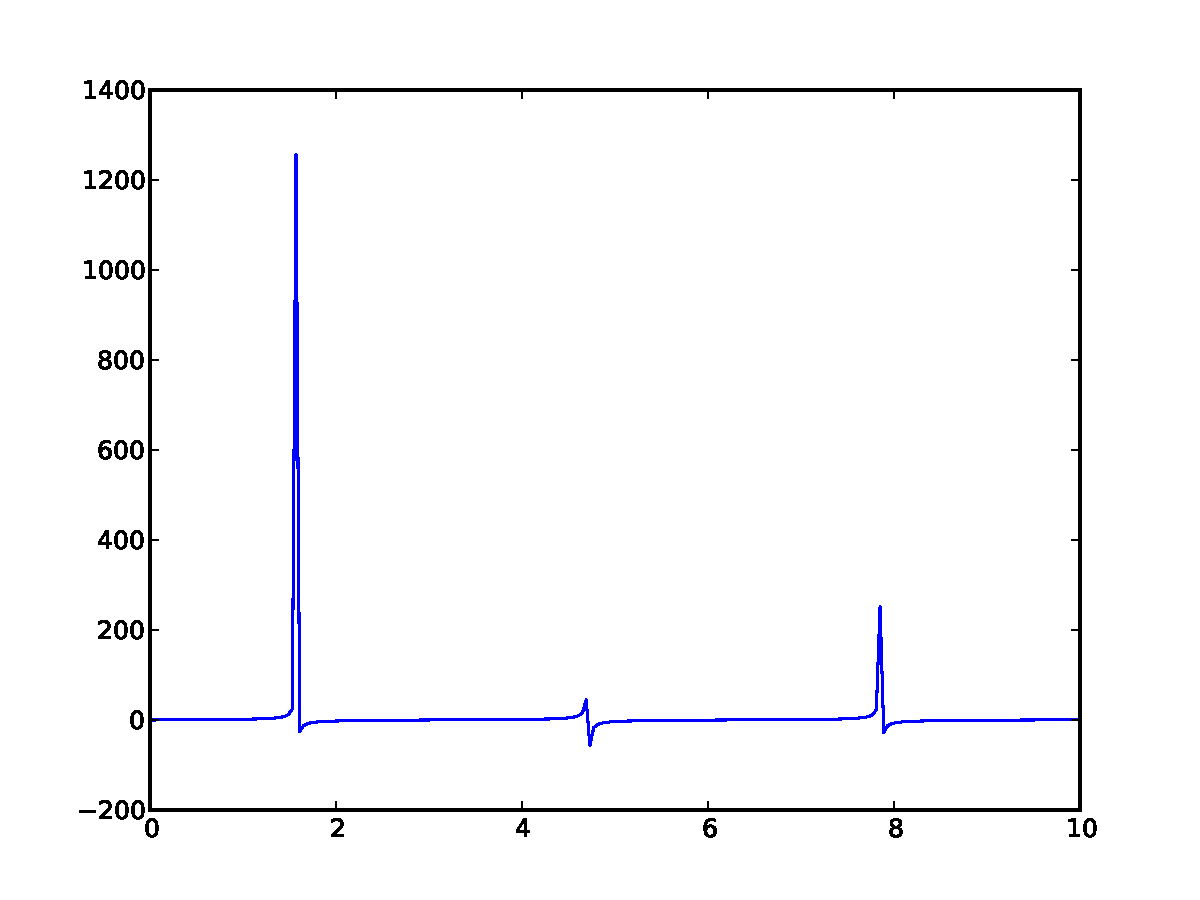
\includegraphics{plotLimits1.pdf}}
\label{chap5/chap5_plot:fig-plotlimits1}\end{figure}

The resulting plot, shown above, doesn't quite look like what you might have expected for \(\tan\theta\) \emph{vs} \(\theta\).  The problem is that \(\tan\theta\) diverges at \(\theta = \pi/2, 3\pi/2, 5\pi/2, ...\), which leads to large spikes in the plots as values in the \code{theta} array come near those values.  Of course, we don't want the plot to extend all the way out to \(\pm\infty\) in the \(y\) direction, nor can it.  Instead, we would like the plot to extend far enough that we get the idea of what is going on as \(y\rightarrow\pm\infty\), but we would still like to see the behavior of the graph near \(y=0\).  We can restrict the range of \code{ytan} values that are plotted using the MatPlotLib function \code{ylim}, as we demonstrate in the script below.

\begin{Verbatim}[commandchars=\\\{\}]
\PYG{k+kn}{import} \PYG{n+nn}{numpy} \PYG{k+kn}{as} \PYG{n+nn}{np}
\PYG{k+kn}{import} \PYG{n+nn}{matplotlib.pyplot} \PYG{k+kn}{as} \PYG{n+nn}{plt}

\PYG{n}{theta} \PYG{o}{=} \PYG{n}{np}\PYG{o}{.}\PYG{n}{arange}\PYG{p}{(}\PYG{l+m+mf}{0.01}\PYG{p}{,} \PYG{l+m+mf}{10.}\PYG{p}{,} \PYG{l+m+mf}{0.04}\PYG{p}{)}
\PYG{n}{ytan} \PYG{o}{=} \PYG{n}{np}\PYG{o}{.}\PYG{n}{tan}\PYG{p}{(}\PYG{n}{theta}\PYG{p}{)}

\PYG{n}{plt}\PYG{o}{.}\PYG{n}{figure}\PYG{p}{(}\PYG{p}{)}
\PYG{n}{plt}\PYG{o}{.}\PYG{n}{plot}\PYG{p}{(}\PYG{n}{theta}\PYG{p}{,} \PYG{n}{ytan}\PYG{p}{)}
\PYG{n}{plt}\PYG{o}{.}\PYG{n}{ylim}\PYG{p}{(}\PYG{o}{\PYGZhy{}}\PYG{l+m+mi}{8}\PYG{p}{,} \PYG{l+m+mi}{8}\PYG{p}{)}         \PYG{c}{\PYGZsh{} restricts range of y axis from \PYGZhy{}8 to +8}
\PYG{n}{plt}\PYG{o}{.}\PYG{n}{axhline}\PYG{p}{(}\PYG{n}{color}\PYG{o}{=}\PYG{l+s}{\PYGZdq{}}\PYG{l+s}{gray}\PYG{l+s}{\PYGZdq{}}\PYG{p}{,} \PYG{n}{zorder}\PYG{o}{=}\PYG{o}{\PYGZhy{}}\PYG{l+m+mi}{1}\PYG{p}{)}

\PYG{n}{plt}\PYG{o}{.}\PYG{n}{show}\PYG{p}{(}\PYG{p}{)}
\end{Verbatim}

The figure produced by this script is shown below.  The plot now looks much more like the familiar \(\tan\theta\) function we know.  We have also include a call to the \code{axline} function to create an \(x\) axis.
\begin{figure}[htbp]
\centering
\capstart

\scalebox{0.800000}{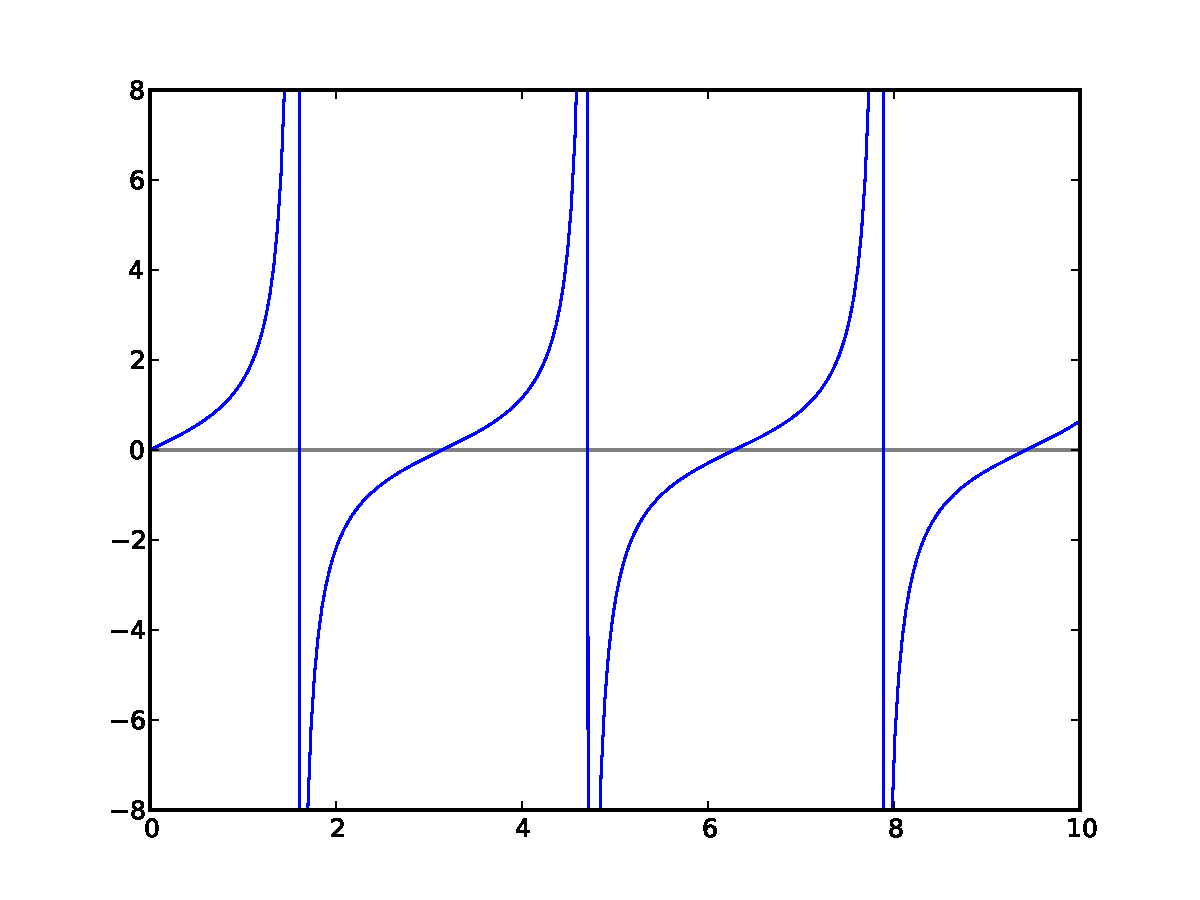
\includegraphics{plotLimits2.pdf}}
\caption{Tangent function (with spurious lines)}\label{chap5/chap5_plot:fig-plotlimits2}\end{figure}

The vertical blue lines at \(\theta = \pi/2, 3\pi/2, 5\pi/2\) should not appear in a plot of \(\tan\theta\) \emph{vs} \(\theta\).  However, they do appear because the \code{plot} function simply draws lines between the data points in the \code{x}-\code{y} arrays provided in its arguments.  Thus, \code{plot} draws a line between the very large positive and negative \code{ytan} values corresponding to the \code{theta} values on either side of \(\pi/2\) where \(\tan\theta\) diverges to \(\pm\infty\).  It would be nice to exclude that line.


\subsubsection{Masked arrays}
\label{chap5/chap5_plot:masked-arrays}
\index{plots!masked arrays}\index{masked arrays}
We can exclude the data points near \(\theta = \pi/2, 3\pi/2, 5\pi/2\) in the above plot, and thus avoid drawing the nearly vertical lines at those points, using NumPy's \emph{masked array} feature.  The code below shows how this is done and produces the graph below.  The masked array feature is implemented in line 6 with a call to NumPy's \code{masked\_where} function in the sub-module \code{ma} (masked array).  Therefore, it is called by writing \code{np.ma.masked\_where}.  The \code{masked\_where} function works as follows.  The first argument sets the condition for masking elements of the array, which is specified by the second argument.  In this case, the function says to mask all elements of the array \code{ytan} (the second argument) where the absolute value of \code{ytan} is greater than 20.  The result is set equal to \code{ytanM}.  When \code{ytanM} is plotted, MatPlotLib's \code{plot} function omits all masked points from the plot.  You can think of it as the \code{plot} function lifting the pen that is drawing the line in the plot when it comes to the masked points in the array \code{ytanM}.
\begin{figure}[htbp]
\centering
\capstart

\scalebox{0.800000}{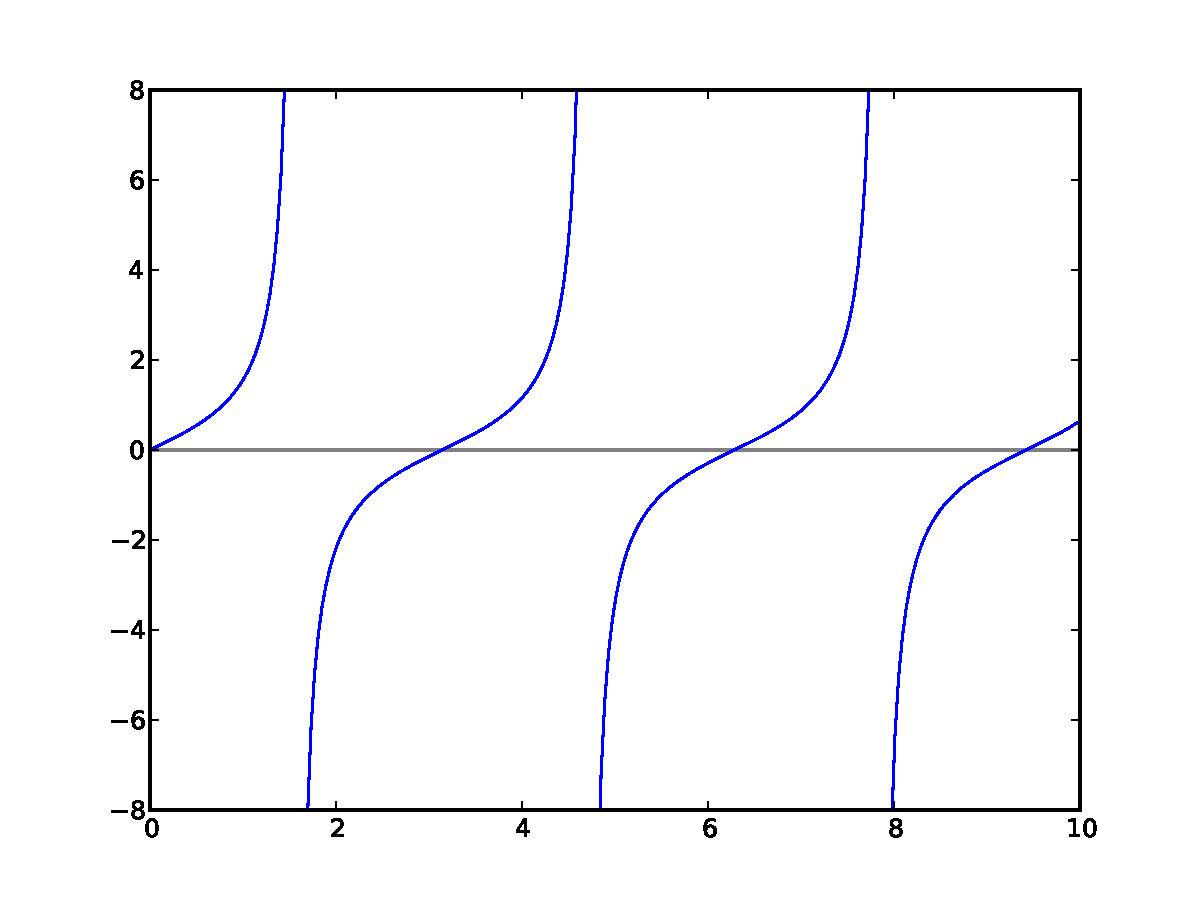
\includegraphics{plotLimits3.pdf}}
\caption{Tangent function}\label{chap5/chap5_plot:fig-plotlimits3}\end{figure}

\begin{Verbatim}[commandchars=\\\{\},numbers=left,firstnumber=1,stepnumber=1]
\PYG{k+kn}{import} \PYG{n+nn}{numpy} \PYG{k+kn}{as} \PYG{n+nn}{np}
\PYG{k+kn}{import} \PYG{n+nn}{matplotlib.pyplot} \PYG{k+kn}{as} \PYG{n+nn}{plt}

\PYG{n}{theta} \PYG{o}{=} \PYG{n}{np}\PYG{o}{.}\PYG{n}{arange}\PYG{p}{(}\PYG{l+m+mf}{0.01}\PYG{p}{,} \PYG{l+m+mf}{10.}\PYG{p}{,} \PYG{l+m+mf}{0.04}\PYG{p}{)}
\PYG{n}{ytan} \PYG{o}{=} \PYG{n}{np}\PYG{o}{.}\PYG{n}{tan}\PYG{p}{(}\PYG{n}{theta}\PYG{p}{)}
\PYG{n}{ytanM} \PYG{o}{=} \PYG{n}{np}\PYG{o}{.}\PYG{n}{ma}\PYG{o}{.}\PYG{n}{masked\PYGZus{}where}\PYG{p}{(}\PYG{n}{np}\PYG{o}{.}\PYG{n}{abs}\PYG{p}{(}\PYG{n}{ytan}\PYG{p}{)}\PYG{o}{\PYGZgt{}}\PYG{l+m+mf}{20.}\PYG{p}{,} \PYG{n}{ytan}\PYG{p}{)}

\PYG{n}{plt}\PYG{o}{.}\PYG{n}{figure}\PYG{p}{(}\PYG{p}{)}
\PYG{n}{plt}\PYG{o}{.}\PYG{n}{plot}\PYG{p}{(}\PYG{n}{theta}\PYG{p}{,} \PYG{n}{ytanM}\PYG{p}{)}
\PYG{n}{plt}\PYG{o}{.}\PYG{n}{ylim}\PYG{p}{(}\PYG{o}{\PYGZhy{}}\PYG{l+m+mi}{8}\PYG{p}{,} \PYG{l+m+mi}{8}\PYG{p}{)}
\PYG{n}{plt}\PYG{o}{.}\PYG{n}{axhline}\PYG{p}{(}\PYG{n}{color}\PYG{o}{=}\PYG{l+s}{\PYGZdq{}}\PYG{l+s}{gray}\PYG{l+s}{\PYGZdq{}}\PYG{p}{,} \PYG{n}{zorder}\PYG{o}{=}\PYG{o}{\PYGZhy{}}\PYG{l+m+mi}{1}\PYG{p}{)}

\PYG{n}{plt}\PYG{o}{.}\PYG{n}{show}\PYG{p}{(}\PYG{p}{)}
\end{Verbatim}


\subsection{Subplots}
\label{chap5/chap5_plot:subplots}
\index{plots!subplots}
Often you want to create two or more graphs and place them next to one another, generally because they are related to each other in some way.  The plot below shows an example of such a plot.  In the top graph, \(\tan\theta\) and \(\sqrt{(8/\theta)^2-1}\) \emph{vs} \(\theta\) are plotted.  The two curves cross each other at the points where \(\tan\theta=\sqrt{(8/\theta)^2-1}\).  In the bottom  \(\cot\theta\) and \(-\sqrt{(8/\theta)^2-1}\) \emph{vs} \(\theta\) are plotted.  These two curves cross each other at the points where \(\cot\theta=-\sqrt{(8/\theta)^2-1}\).
\begin{figure}[htbp]
\centering
\capstart

\scalebox{0.900000}{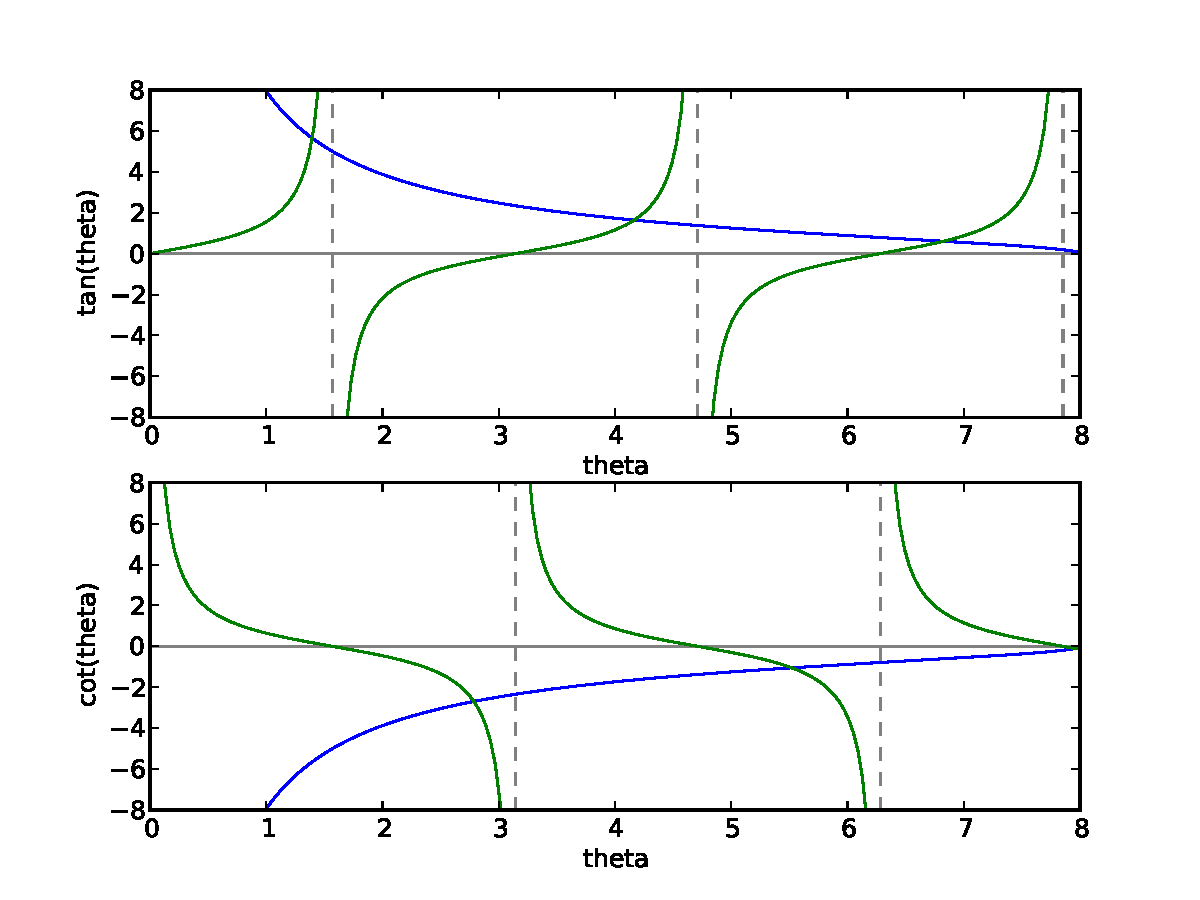
\includegraphics{subplotDemo.pdf}}
\caption{Crossing functions}\label{chap5/chap5_plot:fig-subplotdemo}\end{figure}

The code that produces this plot is provided below.

\begin{Verbatim}[commandchars=\\\{\},numbers=left,firstnumber=1,stepnumber=1]
\PYG{k+kn}{import} \PYG{n+nn}{numpy} \PYG{k+kn}{as} \PYG{n+nn}{np}
\PYG{k+kn}{import} \PYG{n+nn}{matplotlib.pyplot} \PYG{k+kn}{as} \PYG{n+nn}{plt}

\PYG{n}{theta} \PYG{o}{=} \PYG{n}{np}\PYG{o}{.}\PYG{n}{arange}\PYG{p}{(}\PYG{l+m+mf}{0.01}\PYG{p}{,} \PYG{l+m+mf}{8.}\PYG{p}{,} \PYG{l+m+mf}{0.04}\PYG{p}{)}
\PYG{n}{y} \PYG{o}{=} \PYG{n}{np}\PYG{o}{.}\PYG{n}{sqrt}\PYG{p}{(}\PYG{p}{(}\PYG{l+m+mf}{8.}\PYG{o}{/}\PYG{n}{theta}\PYG{p}{)}\PYG{o}{*}\PYG{o}{*}\PYG{l+m+mi}{2}\PYG{o}{\PYGZhy{}}\PYG{l+m+mf}{1.}\PYG{p}{)}
\PYG{n}{ytan} \PYG{o}{=} \PYG{n}{np}\PYG{o}{.}\PYG{n}{tan}\PYG{p}{(}\PYG{n}{theta}\PYG{p}{)}
\PYG{n}{ytan} \PYG{o}{=} \PYG{n}{np}\PYG{o}{.}\PYG{n}{ma}\PYG{o}{.}\PYG{n}{masked\PYGZus{}where}\PYG{p}{(}\PYG{n}{np}\PYG{o}{.}\PYG{n}{abs}\PYG{p}{(}\PYG{n}{ytan}\PYG{p}{)}\PYG{o}{\PYGZgt{}}\PYG{l+m+mf}{20.}\PYG{p}{,} \PYG{n}{ytan}\PYG{p}{)}
\PYG{n}{ycot} \PYG{o}{=} \PYG{l+m+mf}{1.}\PYG{o}{/}\PYG{n}{np}\PYG{o}{.}\PYG{n}{tan}\PYG{p}{(}\PYG{n}{theta}\PYG{p}{)}
\PYG{n}{ycot} \PYG{o}{=} \PYG{n}{np}\PYG{o}{.}\PYG{n}{ma}\PYG{o}{.}\PYG{n}{masked\PYGZus{}where}\PYG{p}{(}\PYG{n}{np}\PYG{o}{.}\PYG{n}{abs}\PYG{p}{(}\PYG{n}{ycot}\PYG{p}{)}\PYG{o}{\PYGZgt{}}\PYG{l+m+mf}{20.}\PYG{p}{,} \PYG{n}{ycot}\PYG{p}{)}

\PYG{n}{plt}\PYG{o}{.}\PYG{n}{figure}\PYG{p}{(}\PYG{l+m+mi}{1}\PYG{p}{)}

\PYG{n}{plt}\PYG{o}{.}\PYG{n}{subplot}\PYG{p}{(}\PYG{l+m+mi}{2}\PYG{p}{,} \PYG{l+m+mi}{1}\PYG{p}{,} \PYG{l+m+mi}{1}\PYG{p}{)}
\PYG{n}{plt}\PYG{o}{.}\PYG{n}{plot}\PYG{p}{(}\PYG{n}{theta}\PYG{p}{,} \PYG{n}{y}\PYG{p}{)}
\PYG{n}{plt}\PYG{o}{.}\PYG{n}{plot}\PYG{p}{(}\PYG{n}{theta}\PYG{p}{,} \PYG{n}{ytan}\PYG{p}{)}
\PYG{n}{plt}\PYG{o}{.}\PYG{n}{ylim}\PYG{p}{(}\PYG{o}{\PYGZhy{}}\PYG{l+m+mi}{8}\PYG{p}{,} \PYG{l+m+mi}{8}\PYG{p}{)}
\PYG{n}{plt}\PYG{o}{.}\PYG{n}{axhline}\PYG{p}{(}\PYG{n}{color}\PYG{o}{=}\PYG{l+s}{\PYGZdq{}}\PYG{l+s}{gray}\PYG{l+s}{\PYGZdq{}}\PYG{p}{,} \PYG{n}{zorder}\PYG{o}{=}\PYG{o}{\PYGZhy{}}\PYG{l+m+mi}{1}\PYG{p}{)}
\PYG{n}{plt}\PYG{o}{.}\PYG{n}{axvline}\PYG{p}{(}\PYG{n}{x}\PYG{o}{=}\PYG{n}{np}\PYG{o}{.}\PYG{n}{pi}\PYG{o}{/}\PYG{l+m+mf}{2.}\PYG{p}{,} \PYG{n}{color}\PYG{o}{=}\PYG{l+s}{\PYGZdq{}}\PYG{l+s}{gray}\PYG{l+s}{\PYGZdq{}}\PYG{p}{,} \PYG{n}{linestyle}\PYG{o}{=}\PYG{l+s}{\PYGZsq{}}\PYG{l+s}{\PYGZhy{}\PYGZhy{}}\PYG{l+s}{\PYGZsq{}}\PYG{p}{,} \PYG{n}{zorder}\PYG{o}{=}\PYG{o}{\PYGZhy{}}\PYG{l+m+mi}{1}\PYG{p}{)}
\PYG{n}{plt}\PYG{o}{.}\PYG{n}{axvline}\PYG{p}{(}\PYG{n}{x}\PYG{o}{=}\PYG{l+m+mf}{3.}\PYG{o}{*}\PYG{n}{np}\PYG{o}{.}\PYG{n}{pi}\PYG{o}{/}\PYG{l+m+mf}{2.}\PYG{p}{,} \PYG{n}{color}\PYG{o}{=}\PYG{l+s}{\PYGZdq{}}\PYG{l+s}{gray}\PYG{l+s}{\PYGZdq{}}\PYG{p}{,} \PYG{n}{linestyle}\PYG{o}{=}\PYG{l+s}{\PYGZsq{}}\PYG{l+s}{\PYGZhy{}\PYGZhy{}}\PYG{l+s}{\PYGZsq{}}\PYG{p}{,} \PYG{n}{zorder}\PYG{o}{=}\PYG{o}{\PYGZhy{}}\PYG{l+m+mi}{1}\PYG{p}{)}
\PYG{n}{plt}\PYG{o}{.}\PYG{n}{axvline}\PYG{p}{(}\PYG{n}{x}\PYG{o}{=}\PYG{l+m+mf}{5.}\PYG{o}{*}\PYG{n}{np}\PYG{o}{.}\PYG{n}{pi}\PYG{o}{/}\PYG{l+m+mf}{2.}\PYG{p}{,} \PYG{n}{color}\PYG{o}{=}\PYG{l+s}{\PYGZdq{}}\PYG{l+s}{gray}\PYG{l+s}{\PYGZdq{}}\PYG{p}{,} \PYG{n}{linestyle}\PYG{o}{=}\PYG{l+s}{\PYGZsq{}}\PYG{l+s}{\PYGZhy{}\PYGZhy{}}\PYG{l+s}{\PYGZsq{}}\PYG{p}{,} \PYG{n}{zorder}\PYG{o}{=}\PYG{o}{\PYGZhy{}}\PYG{l+m+mi}{1}\PYG{p}{)}
\PYG{n}{plt}\PYG{o}{.}\PYG{n}{xlabel}\PYG{p}{(}\PYG{l+s}{\PYGZdq{}}\PYG{l+s}{theta}\PYG{l+s}{\PYGZdq{}}\PYG{p}{)}
\PYG{n}{plt}\PYG{o}{.}\PYG{n}{ylabel}\PYG{p}{(}\PYG{l+s}{\PYGZdq{}}\PYG{l+s}{tan(theta)}\PYG{l+s}{\PYGZdq{}}\PYG{p}{)}

\PYG{n}{plt}\PYG{o}{.}\PYG{n}{subplot}\PYG{p}{(}\PYG{l+m+mi}{2}\PYG{p}{,} \PYG{l+m+mi}{1}\PYG{p}{,} \PYG{l+m+mi}{2}\PYG{p}{)}
\PYG{n}{plt}\PYG{o}{.}\PYG{n}{plot}\PYG{p}{(}\PYG{n}{theta}\PYG{p}{,} \PYG{o}{\PYGZhy{}}\PYG{n}{y}\PYG{p}{)}
\PYG{n}{plt}\PYG{o}{.}\PYG{n}{plot}\PYG{p}{(}\PYG{n}{theta}\PYG{p}{,} \PYG{n}{ycot}\PYG{p}{)}
\PYG{n}{plt}\PYG{o}{.}\PYG{n}{ylim}\PYG{p}{(}\PYG{o}{\PYGZhy{}}\PYG{l+m+mi}{8}\PYG{p}{,} \PYG{l+m+mi}{8}\PYG{p}{)}
\PYG{n}{plt}\PYG{o}{.}\PYG{n}{axhline}\PYG{p}{(}\PYG{n}{color}\PYG{o}{=}\PYG{l+s}{\PYGZdq{}}\PYG{l+s}{gray}\PYG{l+s}{\PYGZdq{}}\PYG{p}{,} \PYG{n}{zorder}\PYG{o}{=}\PYG{o}{\PYGZhy{}}\PYG{l+m+mi}{1}\PYG{p}{)}
\PYG{n}{plt}\PYG{o}{.}\PYG{n}{axvline}\PYG{p}{(}\PYG{n}{x}\PYG{o}{=}\PYG{n}{np}\PYG{o}{.}\PYG{n}{pi}\PYG{p}{,} \PYG{n}{color}\PYG{o}{=}\PYG{l+s}{\PYGZdq{}}\PYG{l+s}{gray}\PYG{l+s}{\PYGZdq{}}\PYG{p}{,} \PYG{n}{linestyle}\PYG{o}{=}\PYG{l+s}{\PYGZsq{}}\PYG{l+s}{\PYGZhy{}\PYGZhy{}}\PYG{l+s}{\PYGZsq{}}\PYG{p}{,} \PYG{n}{zorder}\PYG{o}{=}\PYG{o}{\PYGZhy{}}\PYG{l+m+mi}{1}\PYG{p}{)}
\PYG{n}{plt}\PYG{o}{.}\PYG{n}{axvline}\PYG{p}{(}\PYG{n}{x}\PYG{o}{=}\PYG{l+m+mf}{2.}\PYG{o}{*}\PYG{n}{np}\PYG{o}{.}\PYG{n}{pi}\PYG{p}{,} \PYG{n}{color}\PYG{o}{=}\PYG{l+s}{\PYGZdq{}}\PYG{l+s}{gray}\PYG{l+s}{\PYGZdq{}}\PYG{p}{,} \PYG{n}{linestyle}\PYG{o}{=}\PYG{l+s}{\PYGZsq{}}\PYG{l+s}{\PYGZhy{}\PYGZhy{}}\PYG{l+s}{\PYGZsq{}}\PYG{p}{,} \PYG{n}{zorder}\PYG{o}{=}\PYG{o}{\PYGZhy{}}\PYG{l+m+mi}{1}\PYG{p}{)}
\PYG{n}{plt}\PYG{o}{.}\PYG{n}{xlabel}\PYG{p}{(}\PYG{l+s}{\PYGZdq{}}\PYG{l+s}{theta}\PYG{l+s}{\PYGZdq{}}\PYG{p}{)}
\PYG{n}{plt}\PYG{o}{.}\PYG{n}{ylabel}\PYG{p}{(}\PYG{l+s}{\PYGZdq{}}\PYG{l+s}{cot(theta)}\PYG{l+s}{\PYGZdq{}}\PYG{p}{)}

\PYG{n}{plt}\PYG{o}{.}\PYG{n}{show}\PYG{p}{(}\PYG{p}{)}
\end{Verbatim}

The function  \code{subplot}, called on lines 13 and 24, creates the two subplots in the above figure.   \code{subplot} has three arguments.  The first specifies the number of rows that the figure space is to be divided into; on line 13, it's two.  The second specifies the number of columns that the figure space is to be divided into;  on line 13, it's one.  The third argument specifies which rectangle the will contain the plot specified by the following function calls.  Line 13 specifies that the plotting commands that follow will be act on the first box.  Line 24 specifies that the plotting commands that follow will be act on the second box.

We have also labeled the axes and included dashed vertical lines at the values of \(\theta\) where \(\tan\theta\) and \(\cot\theta\) diverge.


\section{Logarithmic plots}
\label{chap5/chap5_plot:logarithmic-plots}
\index{plots!logarithmic axes}
Data sets can span many orders of magnitude from fractional quantities much smaller than unity to values much larger than unity.  In such cases it is often useful to plot the data on logarithmic axes.


\subsection{Semi-log plots}
\label{chap5/chap5_plot:semi-log-plots}
\index{plots!semi-log}
For data sets that vary exponentially in the independent variable, it is often useful to use one or more logarithmic axes.  Radioactive decay of unstable nuclei, for example, exhibits an exponential decrease in the number of particles emitted from the nuclei as a function of time.  In the plot below, for example, we show the decay of the radioactive isotope Phosphorus-32 over a period of 6 months, where the radioactivity is measured once each week.  Starting at a decay rate of nearly \(10^4\) electrons (counts) per second, the decay rate diminishes to only about 1 count per second after about 6 months or 180 days.  If we plot counts per second as a function of time on a normal plot, as we have done in the plot on the left below, then the count rate is indistinguishable from zero after about 100 days.  On the other hand, if we use a logarithmic axis for the count rate, as we have done in the plot on the right below, then we can follow the count rate well past 100 days and can readily distinguish it from zero.  Moreover, if the data vary exponentially in time, then the data will fall along a straight line, as they do for the case of radioactive decay.
\begin{figure}[htbp]
\centering
\capstart

\scalebox{1.000000}{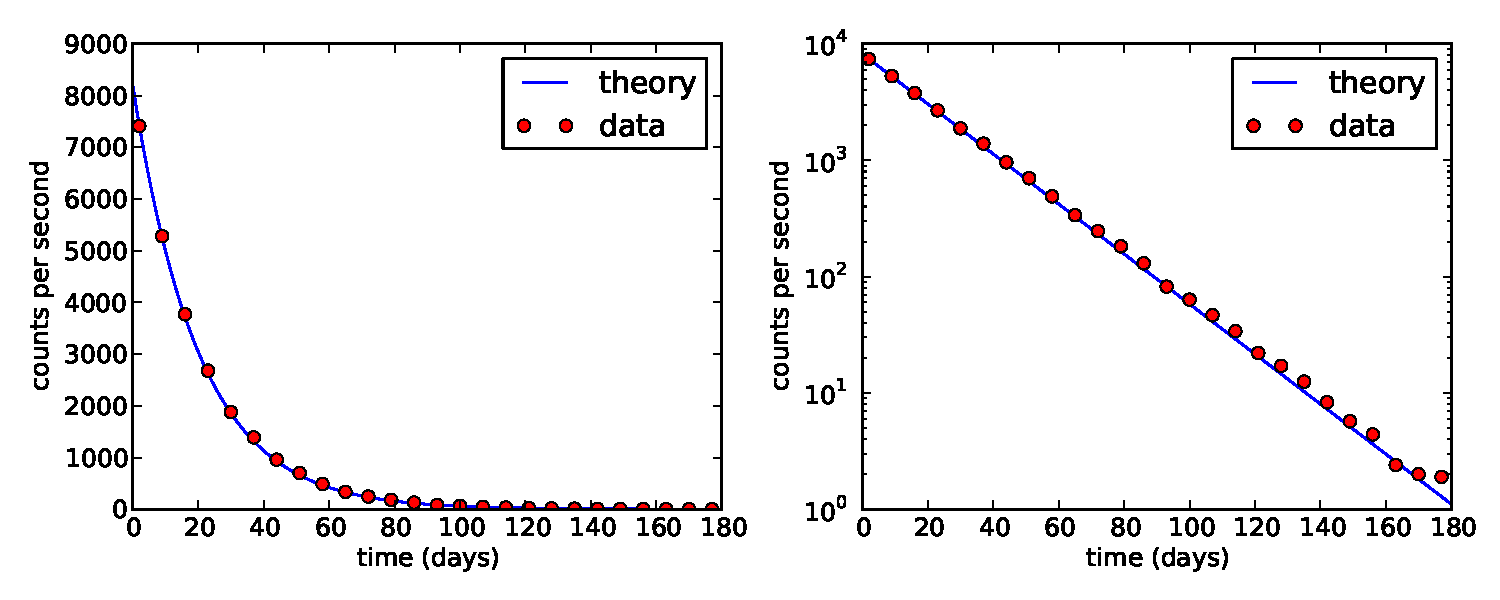
\includegraphics{semilogDemo.pdf}}
\caption{Semi-log plotting}\label{chap5/chap5_plot:fig-semilogdemo}\end{figure}

MatPlotLib provides two functions for making semi-logarithmic plots, \code{semilogx} and \code{semilogy}, for creating plots with logarithmic \(x\) and \(y\) axes, with linear \(y\) and \(x\) axes, respectively.  We illustrate their use in the program below, which made the above plots.

\begin{Verbatim}[commandchars=\\\{\},numbers=left,firstnumber=1,stepnumber=1]
\PYG{k+kn}{import} \PYG{n+nn}{numpy} \PYG{k+kn}{as} \PYG{n+nn}{np}
\PYG{k+kn}{import} \PYG{n+nn}{matplotlib.pyplot} \PYG{k+kn}{as} \PYG{n+nn}{plt}

\PYG{c}{\PYGZsh{} read data from file}
\PYG{n}{time}\PYG{p}{,} \PYG{n}{counts}\PYG{p}{,} \PYG{n}{unc} \PYG{o}{=} \PYG{n}{np}\PYG{o}{.}\PYG{n}{loadtxt}\PYG{p}{(}\PYG{l+s}{\PYGZsq{}}\PYG{l+s}{SemilogDemo.txt}\PYG{l+s}{\PYGZsq{}}\PYG{p}{,} \PYG{n}{unpack}\PYG{o}{=}\PYG{n+nb+bp}{True}\PYG{p}{)}

\PYG{c}{\PYGZsh{} create theoretical fitting curve}
\PYG{n}{tau} \PYG{o}{=} \PYG{l+m+mf}{20.2}      \PYG{c}{\PYGZsh{} Phosphorus\PYGZhy{}32 half life = 14 days; tau = t\PYGZus{}half/ln(2)}
\PYG{n}{N0} \PYG{o}{=} \PYG{l+m+mf}{8200.}       \PYG{c}{\PYGZsh{} Initial count rate (per second)}
\PYG{n}{t} \PYG{o}{=} \PYG{n}{np}\PYG{o}{.}\PYG{n}{linspace}\PYG{p}{(}\PYG{l+m+mi}{0}\PYG{p}{,} \PYG{l+m+mi}{180}\PYG{p}{,} \PYG{l+m+mi}{128}\PYG{p}{)}
\PYG{n}{N} \PYG{o}{=} \PYG{n}{N0} \PYG{o}{*} \PYG{n}{np}\PYG{o}{.}\PYG{n}{exp}\PYG{p}{(}\PYG{o}{\PYGZhy{}}\PYG{n}{t}\PYG{o}{/}\PYG{n}{tau}\PYG{p}{)}

\PYG{c}{\PYGZsh{} create plot}
\PYG{n}{plt}\PYG{o}{.}\PYG{n}{figure}\PYG{p}{(}\PYG{l+m+mi}{1}\PYG{p}{,} \PYG{n}{figsize} \PYG{o}{=} \PYG{p}{(}\PYG{l+m+mi}{10}\PYG{p}{,}\PYG{l+m+mi}{4}\PYG{p}{)} \PYG{p}{)}

\PYG{n}{plt}\PYG{o}{.}\PYG{n}{subplot}\PYG{p}{(}\PYG{l+m+mi}{1}\PYG{p}{,} \PYG{l+m+mi}{2}\PYG{p}{,} \PYG{l+m+mi}{1}\PYG{p}{)}
\PYG{n}{plt}\PYG{o}{.}\PYG{n}{plot}\PYG{p}{(}\PYG{n}{t}\PYG{p}{,} \PYG{n}{N}\PYG{p}{,} \PYG{l+s}{\PYGZsq{}}\PYG{l+s}{b\PYGZhy{}}\PYG{l+s}{\PYGZsq{}}\PYG{p}{,} \PYG{n}{label}\PYG{o}{=}\PYG{l+s}{\PYGZdq{}}\PYG{l+s}{theory}\PYG{l+s}{\PYGZdq{}}\PYG{p}{)}
\PYG{n}{plt}\PYG{o}{.}\PYG{n}{plot}\PYG{p}{(}\PYG{n}{time}\PYG{p}{,} \PYG{n}{counts}\PYG{p}{,} \PYG{l+s}{\PYGZsq{}}\PYG{l+s}{ro}\PYG{l+s}{\PYGZsq{}}\PYG{p}{,} \PYG{n}{label}\PYG{o}{=}\PYG{l+s}{\PYGZdq{}}\PYG{l+s}{data}\PYG{l+s}{\PYGZdq{}}\PYG{p}{)}
\PYG{n}{plt}\PYG{o}{.}\PYG{n}{xlabel}\PYG{p}{(}\PYG{l+s}{\PYGZsq{}}\PYG{l+s}{time (days)}\PYG{l+s}{\PYGZsq{}}\PYG{p}{)}
\PYG{n}{plt}\PYG{o}{.}\PYG{n}{ylabel}\PYG{p}{(}\PYG{l+s}{\PYGZsq{}}\PYG{l+s}{counts per second}\PYG{l+s}{\PYGZsq{}}\PYG{p}{)}
\PYG{n}{plt}\PYG{o}{.}\PYG{n}{legend}\PYG{p}{(}\PYG{n}{loc}\PYG{o}{=}\PYG{l+s}{\PYGZsq{}}\PYG{l+s}{upper right}\PYG{l+s}{\PYGZsq{}}\PYG{p}{)}

\PYG{n}{plt}\PYG{o}{.}\PYG{n}{subplot}\PYG{p}{(}\PYG{l+m+mi}{1}\PYG{p}{,} \PYG{l+m+mi}{2}\PYG{p}{,} \PYG{l+m+mi}{2}\PYG{p}{)}
\PYG{n}{plt}\PYG{o}{.}\PYG{n}{semilogy}\PYG{p}{(}\PYG{n}{t}\PYG{p}{,} \PYG{n}{N}\PYG{p}{,} \PYG{l+s}{\PYGZsq{}}\PYG{l+s}{b\PYGZhy{}}\PYG{l+s}{\PYGZsq{}}\PYG{p}{,} \PYG{n}{label}\PYG{o}{=}\PYG{l+s}{\PYGZdq{}}\PYG{l+s}{theory}\PYG{l+s}{\PYGZdq{}}\PYG{p}{)}
\PYG{n}{plt}\PYG{o}{.}\PYG{n}{semilogy}\PYG{p}{(}\PYG{n}{time}\PYG{p}{,} \PYG{n}{counts}\PYG{p}{,} \PYG{l+s}{\PYGZsq{}}\PYG{l+s}{ro}\PYG{l+s}{\PYGZsq{}}\PYG{p}{,} \PYG{n}{label}\PYG{o}{=}\PYG{l+s}{\PYGZdq{}}\PYG{l+s}{data}\PYG{l+s}{\PYGZdq{}}\PYG{p}{)}
\PYG{n}{plt}\PYG{o}{.}\PYG{n}{xlabel}\PYG{p}{(}\PYG{l+s}{\PYGZsq{}}\PYG{l+s}{time (days)}\PYG{l+s}{\PYGZsq{}}\PYG{p}{)}
\PYG{n}{plt}\PYG{o}{.}\PYG{n}{ylabel}\PYG{p}{(}\PYG{l+s}{\PYGZsq{}}\PYG{l+s}{counts per second}\PYG{l+s}{\PYGZsq{}}\PYG{p}{)}
\PYG{n}{plt}\PYG{o}{.}\PYG{n}{legend}\PYG{p}{(}\PYG{n}{loc}\PYG{o}{=}\PYG{l+s}{\PYGZsq{}}\PYG{l+s}{upper right}\PYG{l+s}{\PYGZsq{}}\PYG{p}{)}

\PYG{n}{plt}\PYG{o}{.}\PYG{n}{tight\PYGZus{}layout}\PYG{p}{(}\PYG{p}{)}

\PYG{c}{\PYGZsh{} display plot on screen}
\PYG{n}{plt}\PYG{o}{.}\PYG{n}{show}\PYG{p}{(}\PYG{p}{)}
\end{Verbatim}

The \code{semilogx} and \code{semilogy} functions work the same way as the \code{plot} function.  You just use one or the other depending on which axis you want to be logarithmic.


\subsubsection{The \texttt{tight\_layout()} function}
\label{chap5/chap5_plot:the-tight-layout-function}
\index{MatPlotLib functions!tight\_layout}
You may have noticed the \code{tight\_layout()} function, called without arguments on line 30 of the program.  This is a convenience function that adjusts the sizes of the plots to make room for the axes labels.  If it is not called, the \(y\)-axis label of the right plot runs into the left plot.  The \code{tight\_layout()} function can also be useful in graphics windows with only one plot sometimes.


\subsection{Log-log plots}
\label{chap5/chap5_plot:log-log-plots}
\index{plots!log-log}
MatPlotLib can also make log-log or double-logarithmic plots using the function \code{loglog}.  It is useful when both the \(x\) and \(y\) data span many orders of magnitude.  Data that are described by a power law \(y=Ax^b\), where \(A\) and \(b\) are constants, appear as straight lines when plotted on a log-log plot.  Again, the \code{loglog} function works just like the \code{plot} function but with logarithmic axes.


\section{More advanced graphical output}
\label{chap5/chap5_plot:more-advanced-graphical-output}
The plotting methods introduced in the previous sections are perfectly adequate for basic plotting and are therefore recommended for simple graphical output.  Here, we introduce an alternative syntax that harnesses the full power of MatPlotLib.  It gives the user more options and greater control.  Perhaps the most efficient way to learn this alternative syntax is to look at an example.  The figure below illustrating {\hyperref[chap5/chap5_plot:multplotdemo]{\emph{Mulitple plots in the same window}}} is produced by the following code:
\begin{figure}[htbp]
\centering
\capstart

\scalebox{0.800000}{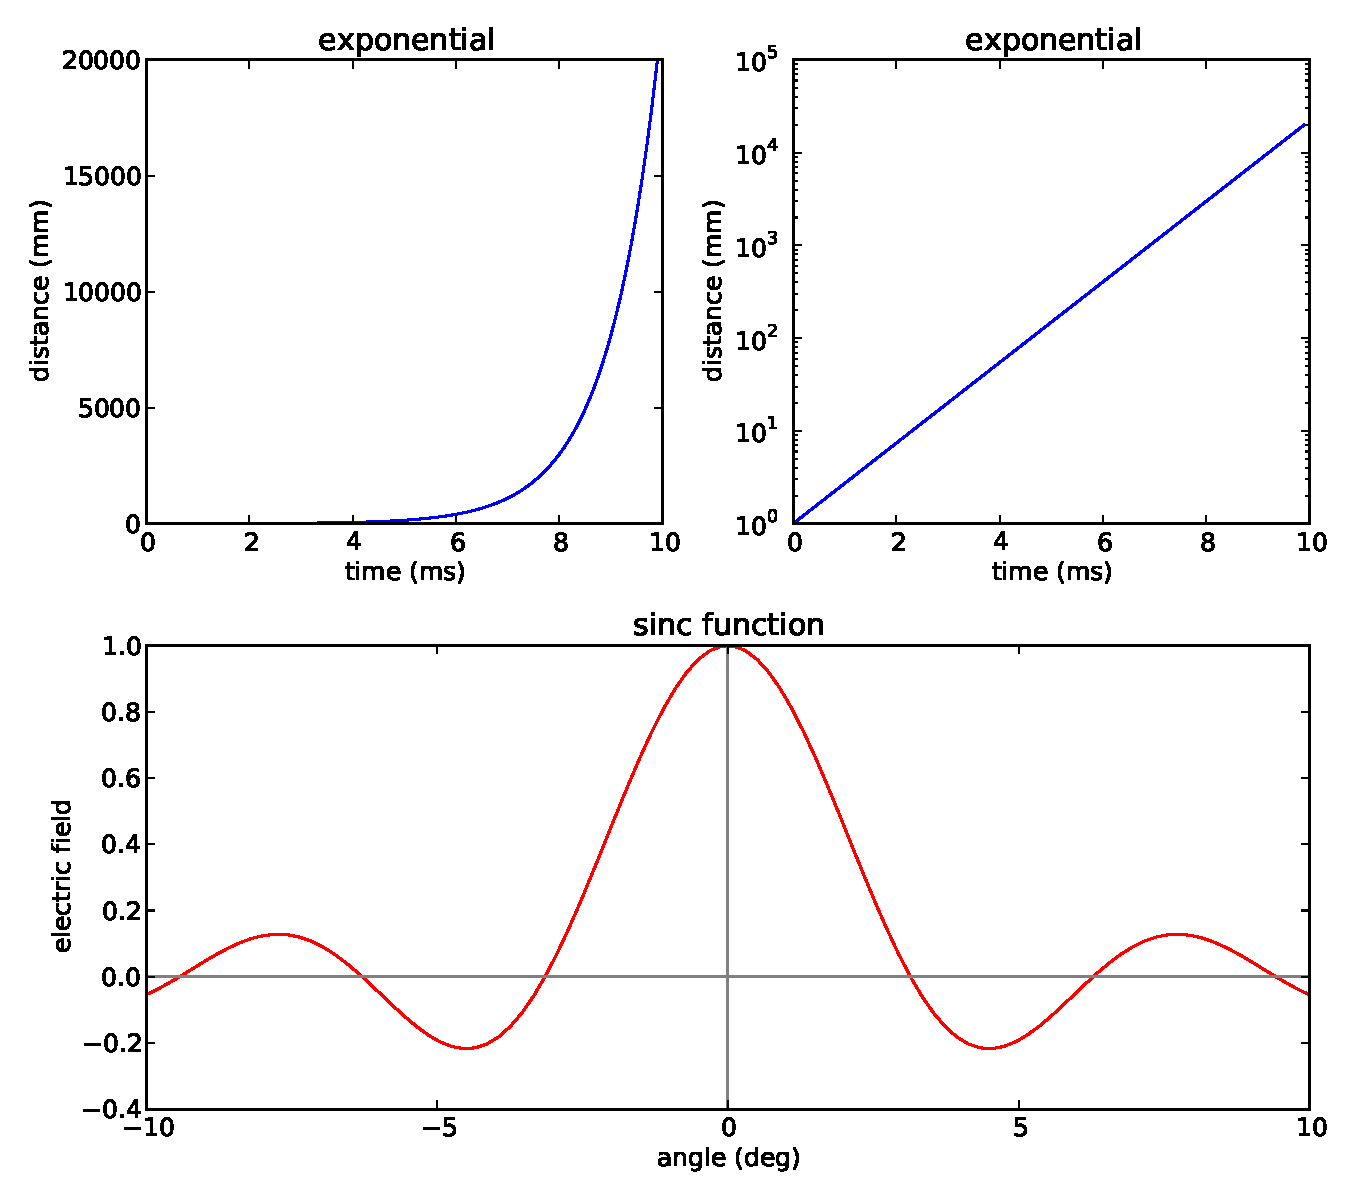
\includegraphics{MultPlotDemo.pdf}}
\caption{Mulitple plots in the same window}\label{chap5/chap5_plot:multplotdemo}\end{figure}

\begin{Verbatim}[commandchars=\\\{\},numbers=left,firstnumber=1,stepnumber=1]
\PYG{c}{\PYGZsh{} Demonstrates the following:}
\PYG{c}{\PYGZsh{}     plotting logarithmic axes}
\PYG{c}{\PYGZsh{}     user\PYGZhy{}defined functions}
\PYG{c}{\PYGZsh{}     \PYGZdq{}where\PYGZdq{} function, NumPy array conditional}

\PYG{k+kn}{import} \PYG{n+nn}{numpy} \PYG{k+kn}{as} \PYG{n+nn}{np}
\PYG{k+kn}{import} \PYG{n+nn}{matplotlib.pyplot} \PYG{k+kn}{as} \PYG{n+nn}{plt}

\PYG{c}{\PYGZsh{} Define the sinc function, with output for x=0 defined}
\PYG{c}{\PYGZsh{} as a special case to avoid division by zero. The code}
\PYG{c}{\PYGZsh{} below defining the sinc function is developed and}
\PYG{c}{\PYGZsh{} explained in Chapter 7, Section 1.}
\PYG{k}{def} \PYG{n+nf}{s}\PYG{p}{(}\PYG{n}{x}\PYG{p}{)}\PYG{p}{:}
  \PYG{n}{a} \PYG{o}{=} \PYG{n}{np}\PYG{o}{.}\PYG{n}{where}\PYG{p}{(}\PYG{n}{x}\PYG{o}{==}\PYG{l+m+mf}{0.}\PYG{p}{,} \PYG{l+m+mf}{1.}\PYG{p}{,} \PYG{n}{np}\PYG{o}{.}\PYG{n}{sin}\PYG{p}{(}\PYG{n}{x}\PYG{p}{)}\PYG{o}{/}\PYG{n}{x}\PYG{p}{)}
  \PYG{k}{return} \PYG{n}{a}

\PYG{c}{\PYGZsh{} create arrays for plotting}
\PYG{n}{x} \PYG{o}{=} \PYG{n}{np}\PYG{o}{.}\PYG{n}{arange}\PYG{p}{(}\PYG{l+m+mf}{0.}\PYG{p}{,} \PYG{l+m+mf}{10.}\PYG{p}{,} \PYG{l+m+mf}{0.1}\PYG{p}{)}
\PYG{n}{y} \PYG{o}{=} \PYG{n}{np}\PYG{o}{.}\PYG{n}{exp}\PYG{p}{(}\PYG{n}{x}\PYG{p}{)}

\PYG{n}{t} \PYG{o}{=} \PYG{n}{np}\PYG{o}{.}\PYG{n}{linspace}\PYG{p}{(}\PYG{o}{\PYGZhy{}}\PYG{l+m+mf}{10.}\PYG{p}{,} \PYG{l+m+mf}{10.}\PYG{p}{,} \PYG{l+m+mi}{100}\PYG{p}{)}
\PYG{n}{z} \PYG{o}{=} \PYG{n}{s}\PYG{p}{(}\PYG{n}{t}\PYG{p}{)}

\PYG{c}{\PYGZsh{} create a figure window}
\PYG{n}{fig} \PYG{o}{=} \PYG{n}{plt}\PYG{o}{.}\PYG{n}{figure}\PYG{p}{(}\PYG{l+m+mi}{1}\PYG{p}{,} \PYG{n}{figsize}\PYG{o}{=}\PYG{p}{(}\PYG{l+m+mi}{9}\PYG{p}{,}\PYG{l+m+mi}{8}\PYG{p}{)}\PYG{p}{)}

\PYG{c}{\PYGZsh{} subplot: linear plot of exponential}
\PYG{n}{ax1} \PYG{o}{=} \PYG{n}{fig}\PYG{o}{.}\PYG{n}{add\PYGZus{}subplot}\PYG{p}{(}\PYG{l+m+mi}{2}\PYG{p}{,}\PYG{l+m+mi}{2}\PYG{p}{,}\PYG{l+m+mi}{1}\PYG{p}{)}
\PYG{n}{ax1}\PYG{o}{.}\PYG{n}{plot}\PYG{p}{(}\PYG{n}{x}\PYG{p}{,} \PYG{n}{y}\PYG{p}{)}
\PYG{n}{ax1}\PYG{o}{.}\PYG{n}{set\PYGZus{}xlabel}\PYG{p}{(}\PYG{l+s}{\PYGZsq{}}\PYG{l+s}{time (ms)}\PYG{l+s}{\PYGZsq{}}\PYG{p}{)}
\PYG{n}{ax1}\PYG{o}{.}\PYG{n}{set\PYGZus{}ylabel}\PYG{p}{(}\PYG{l+s}{\PYGZsq{}}\PYG{l+s}{distance (mm)}\PYG{l+s}{\PYGZsq{}}\PYG{p}{)}
\PYG{n}{ax1}\PYG{o}{.}\PYG{n}{set\PYGZus{}title}\PYG{p}{(}\PYG{l+s}{\PYGZsq{}}\PYG{l+s}{exponential}\PYG{l+s}{\PYGZsq{}}\PYG{p}{)}

\PYG{c}{\PYGZsh{} subplot: semi\PYGZhy{}log plot of exponential}
\PYG{n}{ax2} \PYG{o}{=} \PYG{n}{fig}\PYG{o}{.}\PYG{n}{add\PYGZus{}subplot}\PYG{p}{(}\PYG{l+m+mi}{2}\PYG{p}{,}\PYG{l+m+mi}{2}\PYG{p}{,}\PYG{l+m+mi}{2}\PYG{p}{)}
\PYG{n}{ax2}\PYG{o}{.}\PYG{n}{plot}\PYG{p}{(}\PYG{n}{x}\PYG{p}{,} \PYG{n}{y}\PYG{p}{)}
\PYG{n}{ax2}\PYG{o}{.}\PYG{n}{set\PYGZus{}yscale}\PYG{p}{(}\PYG{l+s}{\PYGZsq{}}\PYG{l+s}{log}\PYG{l+s}{\PYGZsq{}}\PYG{p}{)}
\PYG{n}{ax2}\PYG{o}{.}\PYG{n}{set\PYGZus{}xlabel}\PYG{p}{(}\PYG{l+s}{\PYGZsq{}}\PYG{l+s}{time (ms)}\PYG{l+s}{\PYGZsq{}}\PYG{p}{)}
\PYG{n}{ax2}\PYG{o}{.}\PYG{n}{set\PYGZus{}ylabel}\PYG{p}{(}\PYG{l+s}{\PYGZsq{}}\PYG{l+s}{distance (mm)}\PYG{l+s}{\PYGZsq{}}\PYG{p}{)}
\PYG{n}{ax2}\PYG{o}{.}\PYG{n}{set\PYGZus{}title}\PYG{p}{(}\PYG{l+s}{\PYGZsq{}}\PYG{l+s}{exponential}\PYG{l+s}{\PYGZsq{}}\PYG{p}{)}

\PYG{c}{\PYGZsh{} subplot: wide subplot of sinc function}
\PYG{n}{ax3} \PYG{o}{=} \PYG{n}{fig}\PYG{o}{.}\PYG{n}{add\PYGZus{}subplot}\PYG{p}{(}\PYG{l+m+mi}{2}\PYG{p}{,}\PYG{l+m+mi}{1}\PYG{p}{,}\PYG{l+m+mi}{2}\PYG{p}{)}
\PYG{n}{ax3}\PYG{o}{.}\PYG{n}{plot}\PYG{p}{(}\PYG{n}{t}\PYG{p}{,} \PYG{n}{z}\PYG{p}{,} \PYG{l+s}{\PYGZsq{}}\PYG{l+s}{r}\PYG{l+s}{\PYGZsq{}}\PYG{p}{)}
\PYG{n}{ax3}\PYG{o}{.}\PYG{n}{axhline}\PYG{p}{(}\PYG{n}{color}\PYG{o}{=}\PYG{l+s}{\PYGZsq{}}\PYG{l+s}{gray}\PYG{l+s}{\PYGZsq{}}\PYG{p}{)}
\PYG{n}{ax3}\PYG{o}{.}\PYG{n}{axvline}\PYG{p}{(}\PYG{n}{color}\PYG{o}{=}\PYG{l+s}{\PYGZsq{}}\PYG{l+s}{gray}\PYG{l+s}{\PYGZsq{}}\PYG{p}{)}
\PYG{n}{ax3}\PYG{o}{.}\PYG{n}{set\PYGZus{}xlabel}\PYG{p}{(}\PYG{l+s}{\PYGZsq{}}\PYG{l+s}{angle (deg)}\PYG{l+s}{\PYGZsq{}}\PYG{p}{)}
\PYG{n}{ax3}\PYG{o}{.}\PYG{n}{set\PYGZus{}ylabel}\PYG{p}{(}\PYG{l+s}{\PYGZsq{}}\PYG{l+s}{electric field}\PYG{l+s}{\PYGZsq{}}\PYG{p}{)}
\PYG{n}{ax3}\PYG{o}{.}\PYG{n}{set\PYGZus{}title}\PYG{p}{(}\PYG{l+s}{\PYGZsq{}}\PYG{l+s}{sinc function}\PYG{l+s}{\PYGZsq{}}\PYG{p}{)}

\PYG{c}{\PYGZsh{} Adjusts white space to avoid collisions between subplots}
\PYG{n}{fig}\PYG{o}{.}\PYG{n}{tight\PYGZus{}layout}\PYG{p}{(}\PYG{p}{)}
\PYG{n}{plt}\PYG{o}{.}\PYG{n}{show}\PYG{p}{(}\PYG{p}{)}
\end{Verbatim}

After defining several arrays for plotting, the above program opens a figure window in line 23 with the statement

\begin{Verbatim}[commandchars=\\\{\}]
\PYG{n}{fig} \PYG{o}{=} \PYG{n}{plt}\PYG{o}{.}\PYG{n}{figure}\PYG{p}{(}\PYG{n}{figsize}\PYG{o}{=}\PYG{p}{(}\PYG{l+m+mi}{9}\PYG{p}{,}\PYG{l+m+mi}{8}\PYG{p}{)}\PYG{p}{)}
\end{Verbatim}

The MatPlotLib statement above creates a \textbf{Figure} object, assigns it the name \code{fig}, and opens a blank figure window.  Thus, just as we give lists, arrays, and numbers variable names (\emph{e.g.} \code{a = {[}1, 2, 5, 7{]}}, \code{dd = np.array({[}2.3, 5.1, 3.9{]})}, or \code{st = 4.3}), we can give a figure object and the window in creates a name: here it is \code{fig}.  In fact we can use the \code{figure} function to open up multiple figure objects with different figure windows.  The statements

\begin{Verbatim}[commandchars=\\\{\}]
\PYG{n}{fig1} \PYG{o}{=} \PYG{n}{plt}\PYG{o}{.}\PYG{n}{figure}\PYG{p}{(}\PYG{p}{)}
\PYG{n}{fig2} \PYG{o}{=} \PYG{n}{plt}\PYG{o}{.}\PYG{n}{figure}\PYG{p}{(}\PYG{p}{)}
\end{Verbatim}

open up two separate windows, one named \code{fig1} and the other \code{fig2}.  We can then use the names \code{fig1} and \code{fig2} to plot things in either window.  The \code{figure} function need not take any arguments if you are satisfied with the default settings such as the figure size and the background color.  On the other hane, by supplying one or more keyword arguments, you can customize the figure size, the background color, and a few other properties.  For example, in the program listing (line 23), the keyword argument \code{figsize} sets the width and height of the figure window; the default size is \code{(8, 6)}; in our program we set it to \code{(9, 8)}, which is a bit wider and higher than the default size.  In the example above, we also choose to open only a single window, hence the single \code{figure} call.

The \code{fig.add\_subplot(2,2,1)} in line 30 is a MatPlotLib function that divides the figure window into 2 rows (the first argument) and 2 columns (the second argument).  The third argument creates a subplot in the first of the 4 subregions (\emph{i.e.} of the 2 rows \(\times\) 2 columns) created by the \code{fig.add\_subplot(2,2,1)} call.   To see how this works, type the following code into a Python module and run it:

\begin{Verbatim}[commandchars=\\\{\},numbers=left,firstnumber=1,stepnumber=1]
\PYG{k+kn}{import} \PYG{n+nn}{numpy} \PYG{k+kn}{as} \PYG{n+nn}{np}
\PYG{k+kn}{import} \PYG{n+nn}{matplotlib.pyplot} \PYG{k+kn}{as} \PYG{n+nn}{plt}

\PYG{n}{fig} \PYG{o}{=} \PYG{n}{plt}\PYG{o}{.}\PYG{n}{figure}\PYG{p}{(}\PYG{n}{figsize}\PYG{o}{=}\PYG{p}{(}\PYG{l+m+mi}{9}\PYG{p}{,}\PYG{l+m+mi}{8}\PYG{p}{)}\PYG{p}{)}
\PYG{n}{ax1} \PYG{o}{=} \PYG{n}{fig}\PYG{o}{.}\PYG{n}{add\PYGZus{}subplot}\PYG{p}{(}\PYG{l+m+mi}{2}\PYG{p}{,}\PYG{l+m+mi}{2}\PYG{p}{,}\PYG{l+m+mi}{1}\PYG{p}{)}

\PYG{n}{plt}\PYG{o}{.}\PYG{n}{show}\PYG{p}{(}\PYG{p}{)}
\end{Verbatim}

You should get a figure window with axes drawn in the upper left quadrant.  The \code{fig.} prefix used with the \code{add\_subplot(2,2,1)} function directs Python to draw these axes in the figure window named \code{fig}.  If we had opened two figure windows, changing the prefix to correspond to the name of one or the other of the figure windows would direct the axes to be drawn in the appropriate window.  Writing \code{ax1 = fig.add\_subplot(2,2,1)} assigns the name ax1 to the axes in the upper left quadrant of the figure window.

The \code{ax1.plot(x, y)} in line 27 directs Python to plot the previously-defined \code{x} and \code{y} arrays onto the axes named \code{ax1}. The \code{ax2 = fig.add\_subplot(2,2,2)} draws axes in the second, or upper right, quadrant of the figure window. The \code{ax3 = fig.add\_subplot(2,1,2)} divides the figure window into 2 rows (first argument) and 1 column (second argument), creates axes in the second or these two sections, and assigns those axes (\emph{i.e.} that subplot) the name \code{ax3}.  That is, it divides the figure window into 2 halves, top and bottom, and then draws axes in the half number 2 (the third argument), or lower half of the figure window.

You may have noticed in above code that some of the function calls are a bit different from those used before: \code{xlabel(’time (ms)’)} becomes \code{set\_xlabel(’time (ms)’)}, \code{title(’exponential’)} becomes \code{set\_title(’exponential’)}, \emph{etc.}

The call \code{ax2.set\_yscale('log')} sets the \(y\)-axes in the second plot to be logarithmic, thus creating a semi-log plot.  Creating properly-labeled logarthmic axes like this is more straightforward with the advanced syntax illustrated in the above example.

Using the prefixes \code{ax1}, \code{ax2}, or \code{ax3}, direct graphical instructions to their respective subplots.  By creating and specifying names for the different figure windows and subplots within them, you access the different plot windows more efficiently.  For example, the following code makes four identical subplots in a single figure window using a \code{for} loop.

\begin{Verbatim}[commandchars=\\\{\}]
\PYG{g+gp}{In [1]: }\PYG{n}{fig} \PYG{o}{=} \PYG{n}{figure}\PYG{p}{(}\PYG{p}{)}

\PYG{g+gp}{In [2]: }\PYG{n}{ax1} \PYG{o}{=} \PYG{n}{fig}\PYG{o}{.}\PYG{n}{add\PYGZus{}subplot}\PYG{p}{(}\PYG{l+m+mi}{221}\PYG{p}{)}

\PYG{g+gp}{In [3]: }\PYG{n}{ax2} \PYG{o}{=} \PYG{n}{fig}\PYG{o}{.}\PYG{n}{add\PYGZus{}subplot}\PYG{p}{(}\PYG{l+m+mi}{222}\PYG{p}{)}

\PYG{g+gp}{In [4]: }\PYG{n}{ax3} \PYG{o}{=} \PYG{n}{fig}\PYG{o}{.}\PYG{n}{add\PYGZus{}subplot}\PYG{p}{(}\PYG{l+m+mi}{223}\PYG{p}{)}

\PYG{g+gp}{In [5]: }\PYG{n}{ax4} \PYG{o}{=} \PYG{n}{fig}\PYG{o}{.}\PYG{n}{add\PYGZus{}subplot}\PYG{p}{(}\PYG{l+m+mi}{224}\PYG{p}{)}

\PYG{g+gp}{In [6]: }\PYG{k}{for} \PYG{n}{ax} \PYG{o+ow}{in} \PYG{p}{[}\PYG{n}{ax1}\PYG{p}{,} \PYG{n}{ax2}\PYG{p}{,} \PYG{n}{ax3}\PYG{p}{,} \PYG{n}{ax4}\PYG{p}{]}\PYG{p}{:}
\PYG{g+gp}{   ...:}     \PYG{n}{ax}\PYG{o}{.}\PYG{n}{plot}\PYG{p}{(}\PYG{p}{[}\PYG{l+m+mi}{3}\PYG{p}{,}\PYG{l+m+mi}{5}\PYG{p}{,}\PYG{l+m+mi}{8}\PYG{p}{]}\PYG{p}{,}\PYG{p}{[}\PYG{l+m+mi}{6}\PYG{p}{,}\PYG{l+m+mi}{3}\PYG{p}{,}\PYG{l+m+mi}{1}\PYG{p}{]}\PYG{p}{)}

\PYG{g+gp}{In [7]: }\PYG{n}{show}\PYG{p}{(}\PYG{p}{)}
\end{Verbatim}
\newpage

\section{Exercises}
\label{chap5/chap5_plot:exercises}\begin{enumerate}
\item {} 
Plot the function \(y=3x^2\) for \(-1 \le x \le 3\) as a continuous line.  Include enough points so that the curve you plot appears smooth.  Label the axes \(x\) and \(y\).

\item {} 
Plot the following function for \(-15 \le x \le 15\):
\begin{gather}
\begin{split}y = \frac{\cos x}{1+\frac{1}{5}x^2}\end{split}\notag
\end{gather}
Include enough points so that the curve you plot appears smooth.  Label the axes \(x\) and \(y\).

\item {} 
Plot the functions \(\sin x\) and \(\cos x\) \emph{vs} \(x\) on the same plot with \(x\) going from \(-\pi\) to \(\pi\).  Make sure the limits of \(x\)-axis do not extend beyond the limits of the data.  Plot \(\sin x\) in the color green and \(\cos x\) in the color black and include a legend to label the two curves.  Place the legend within the plot, but such that it does not cover either of the sine or cosine traces.

\item {} 
Create a data file with the data shown below.
\begin{enumerate}
\item {} 
Read the data into Python program and plot \(t\) \emph{vs} \(y\) using circles for data points with error bars.  Use the data in the \code{dy} column as the error estimates for the \(y\) data.  Label the horizontal and vertical axes ``time (s)'' and ``position (cm)''.

\item {} 
On the same graph, plot the function below as a smooth line.  Make the line pass \emph{behind} the data points.
\begin{gather}
\begin{split}y(t) = \left[3 +
       \frac{1}{2}\sin\frac{\pi t}{5}\right]
       t\, e^{-t/10}\end{split}\notag
\end{gather}
\begin{Verbatim}[commandchars=\\\{\},numbers=left,firstnumber=1,stepnumber=1]
Data for Exercise 4
Date: 16\PYGZhy{}Aug\PYGZhy{}2013
Data taken by Lauren and John

 t      d       dy
 1.0    2.94    0.7
 4.5    8.29    1.2
 8.0    9.36    1.2
11.5   11.60    1.4
15.0    9.32    1.3
18.5    7.75    1.1
22.0    8.06    1.2
25.5    5.60    1.0
29.0    4.50    0.8
32.5    4.01    0.8
36.0    2.62    0.7
39.5    1.70    0.6
43.0    2.03    0.6
\end{Verbatim}

\end{enumerate}

\item {} 
Use MatPlotLib's function \code{hist} along with NumPy's function's \code{random.rand} and \code{random.randn} to create the histogram graphs shown in Fig. {\hyperref[chap3/chap3_arrays:fig-randhistos]{\emph{Histograms of random numbers.}}}

\item {} 
Plot force \emph{vs} distance with error bars using the following data:

\begin{Verbatim}[commandchars=\\\{\}]
\PYG{n}{d}\PYG{o}{=}\PYG{n}{np}\PYG{o}{.}\PYG{n}{array}\PYG{p}{(}\PYG{p}{[}\PYG{l+m+mf}{0.38}\PYG{p}{,} \PYG{l+m+mf}{0.64}\PYG{p}{,} \PYG{l+m+mf}{0.91}\PYG{p}{,} \PYG{l+m+mf}{1.26}\PYG{p}{,} \PYG{l+m+mf}{1.41}\PYG{p}{,} \PYG{l+m+mf}{1.66}\PYG{p}{,} \PYG{l+m+mf}{1.90}\PYG{p}{,} \PYG{l+m+mf}{2.18}\PYG{p}{]}\PYG{p}{)}
\PYG{n}{f}\PYG{o}{=}\PYG{n}{np}\PYG{o}{.}\PYG{n}{array}\PYG{p}{(}\PYG{p}{[}\PYG{l+m+mf}{1.4}\PYG{p}{,} \PYG{l+m+mf}{1.65}\PYG{p}{,} \PYG{l+m+mf}{3.0}\PYG{p}{,} \PYG{l+m+mf}{3.95}\PYG{p}{,} \PYG{l+m+mf}{4.3}\PYG{p}{,} \PYG{l+m+mf}{5.20}\PYG{p}{,} \PYG{l+m+mf}{6.85}\PYG{p}{,} \PYG{l+m+mf}{7.4}\PYG{p}{]}\PYG{p}{)}
\PYG{n}{df}\PYG{o}{=}\PYG{n}{np}\PYG{o}{.}\PYG{n}{array}\PYG{p}{(}\PYG{p}{[} \PYG{l+m+mf}{0.4}\PYG{p}{,} \PYG{l+m+mf}{0.5}\PYG{p}{,} \PYG{l+m+mf}{0.4}\PYG{p}{,} \PYG{l+m+mf}{0.5}\PYG{p}{,} \PYG{l+m+mf}{0.6}\PYG{p}{,} \PYG{l+m+mf}{0.5}\PYG{p}{,} \PYG{l+m+mf}{0.5}\PYG{p}{,} \PYG{l+m+mf}{0.4}\PYG{p}{]}\PYG{p}{)}
\end{Verbatim}

Your plot should also include a visual straight ``best fit'' to the data as well as visual ``fits'' that give the smallest and largest slopes consistent with the data.  Note, you only need two points to define a straight line so the straight lines you draw on the plot should be arrays of length 2 and no longer.  All of your fitted lines should lie \emph{behind} the data.  Try to make your plot look like the one below.  \emph{In addition}, add a legend to your plot the gives the slope with its uncertainty obtained from your visual fits to the data.
\begin{figure}[htbp]
\centering

\scalebox{0.800000}{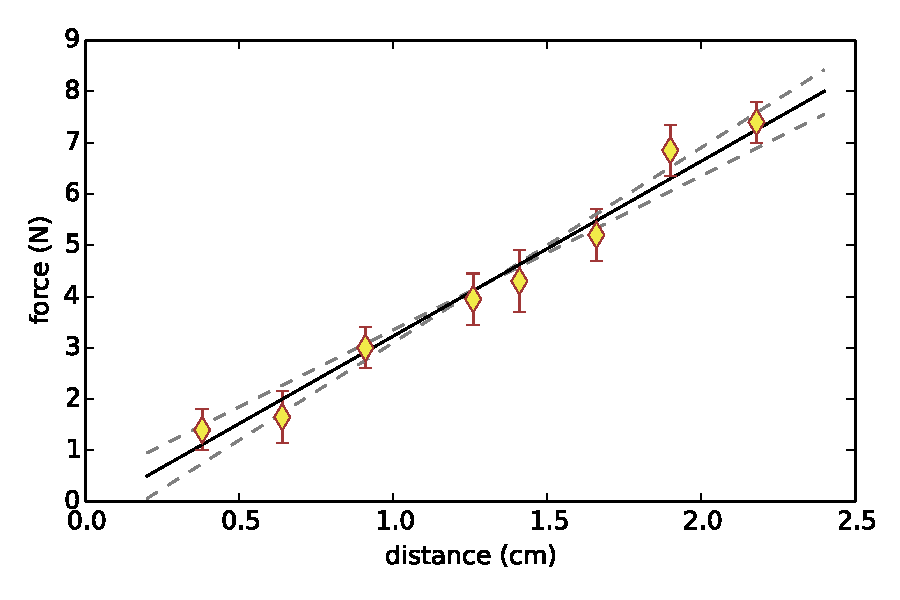
\includegraphics{LinearData.pdf}}
\label{chap5/chap5_plot:fig-lineardata}\end{figure}

The web page \href{http://matplotlib.org/api/pyplot\_summary.html}{http://matplotlib.org/api/pyplot\_summary.html} gives a summary of the main plotting commands available in MatPlotLib.  The two important ones here are \code{plot} and \code{errorbar}, which make regular plots and plots with error bars, respectively.  You will find the following keyword arguments useful: \code{yerr}, \code{ls}, \code{marker}, \code{mfc}, \code{mec}, \code{ms}, and \code{ecolor}, which you can find described by clicking on the \code{errorbar} function link on the web page cited above.

\item {} 
The data file below shows data obtained for the displacement (position) \emph{vs} time of a falling object, together with the estimated uncertainty in the displacement.
\begin{quote}

\begin{Verbatim}[commandchars=\\\{\},numbers=left,firstnumber=1,stepnumber=1]
Measurements of fall velocity vs time
Taken by A.P. Crawford and S.M. Torres
19\PYGZhy{}Sep\PYGZhy{}13
time (s)    position (m)    uncertainty (m)
 0.0            0.0             0.04
 0.5            1.3             0.12
 1.0            5.1             0.2
 1.5           10.9             0.3
 2.0           18.9             0.4
 2.5           28.7             0.4
 3.0           40.3             0.5
 3.5           53.1             0.6
 4.0           67.5             0.6
 4.5           82.3             0.6
 5.0           97.6             0.7
 5.5          113.8             0.7
 6.0          131.2             0.7
 6.5          148.5             0.7
 7.0          166.2             0.7
 7.5          184.2             0.7
 8.0          201.6             0.7
 8.5          220.1             0.7
 9.0          238.3             0.7
 9.5          256.5             0.7
10.0          275.6             0.8
\end{Verbatim}
\end{quote}
\begin{enumerate}
\item {} 
Use these data to calculate the velocity and acceleration (in a Python program \code{.py} file), together with their uncertainties propagated from the displacement \emph{vs} time uncertainties.  Be sure to calculate time arrays corresponding the midpoint in time between the two displacements or velocities for the velocity and acceleration arrays, respectively.

\item {} 
In a single window frame, make three vertically stacked plots of the displacement, velocity, and acceleration \emph{vs} time.  Show the error bars on the different plots.  Make sure that the time axes of all three plots cover the same range of times. Why do the relative sizes of the error bars grow progressively greater as one progresses from displacement to velocity to acceleration?

\end{enumerate}

\end{enumerate}


\chapter{Conditionals and Loops}
\label{chap6/chap6_loopsconds:chap6}\label{chap6/chap6_loopsconds:conditionals-and-loops}\label{chap6/chap6_loopsconds::doc}
Computer programs are useful for performing repetitive tasks.  Without complaining, getting bored, or growing tired, they can repetitively perform the same calculations with minor, but important, variations over and over again.  Humans share with computers none of these qualities.  And so we humans employ computers to perform the massive repetitive tasks we would rather avoid. However, we need efficient ways of telling the computer to do these repetitive tasks; we don't want to have stop to tell the computer each time it finishes one iteration of a task to do the task again, but for a slightly different case.  We want to tell it once, ``Do this task 1000 times with slightly different conditions and report back to me when you are done.''  This is what \textbf{loops} were made for.

In the course of doing these repetitive tasks, computers often need to make decisions.  In general, we don't want the computer to stop and ask us what it should do if a certain result is obtained from its calculations.  We might prefer to say,  ``Look, if you get result A during your calculations, do this, otherwise, do this other thing.''  That is, we often want to tell the computer ahead of time what to do if it encounters different situations.  This is what \textbf{conditionals} were made for.

Conditionals and loops control the flow of a program.  They are essential to performing virtually any significant computational task.  Python, like most computer languages, provides a variety of ways of implementing loops and conditionals.

\index{conditionals}

\section{Conditionals}
\label{chap6/chap6_loopsconds:index-0}\label{chap6/chap6_loopsconds:conditionals}
Conditional statements allow a computer program to take different actions based on whether some condition, or set of conditions is true or false.  In this way, the programmer can control the flow of a program.


\subsection{\texttt{if}, \texttt{elif}, and \texttt{else} statements}
\label{chap6/chap6_loopsconds:if-elif-and-else-statements}
The \code{if}, \code{elif}, and \code{else} statements are used to define conditionals in Python.  We illustrate their use with a few examples.


\subsubsection{\texttt{if}-\texttt{elif}-\texttt{else} example}
\label{chap6/chap6_loopsconds:if-elif-else-example}
Suppose we want to know if the solutions to the quadratic equation
\begin{gather}
\begin{split}ax^2 + bx + c = 0\end{split}\notag
\end{gather}
are real, imaginary, or complex for a given set of coefficients \(a\), \(b\), and \(c\).  Of course, the answer to that question depends on the value of the discriminant \(d=b^2-4ac\).  The solutions are real if \(d \ge 0\), imaginary if \(b=0\) and \(d < 0\), and complex if \(b \ne 0\) and \(d < 0\).  The program below implements the above logic in a Python program.

\begin{Verbatim}[commandchars=\\\{\},numbers=left,firstnumber=1,stepnumber=1]
\PYG{n}{a} \PYG{o}{=} \PYG{n+nb}{float}\PYG{p}{(}\PYG{n+nb}{raw\PYGZus{}input}\PYG{p}{(}\PYG{l+s}{\PYGZdq{}}\PYG{l+s}{What is the coefficients a? }\PYG{l+s}{\PYGZdq{}}\PYG{p}{)}\PYG{p}{)}
\PYG{n}{b} \PYG{o}{=} \PYG{n+nb}{float}\PYG{p}{(}\PYG{n+nb}{raw\PYGZus{}input}\PYG{p}{(}\PYG{l+s}{\PYGZdq{}}\PYG{l+s}{What is the coefficients b? }\PYG{l+s}{\PYGZdq{}}\PYG{p}{)}\PYG{p}{)}
\PYG{n}{c} \PYG{o}{=} \PYG{n+nb}{float}\PYG{p}{(}\PYG{n+nb}{raw\PYGZus{}input}\PYG{p}{(}\PYG{l+s}{\PYGZdq{}}\PYG{l+s}{What is the coefficients c? }\PYG{l+s}{\PYGZdq{}}\PYG{p}{)}\PYG{p}{)}

\PYG{n}{d} \PYG{o}{=} \PYG{n}{b}\PYG{o}{*}\PYG{n}{b} \PYG{o}{\PYGZhy{}} \PYG{l+m+mf}{4.}\PYG{o}{*}\PYG{n}{a}\PYG{o}{*}\PYG{n}{c}

\PYG{k}{if} \PYG{n}{d} \PYG{o}{\PYGZgt{}}\PYG{o}{=} \PYG{l+m+mf}{0.0}\PYG{p}{:}
    \PYG{k}{print}\PYG{p}{(}\PYG{l+s}{\PYGZdq{}}\PYG{l+s}{Solutions are real}\PYG{l+s}{\PYGZdq{}}\PYG{p}{)}         \PYG{c}{\PYGZsh{} block 1}
\PYG{k}{elif} \PYG{n}{b} \PYG{o}{==} \PYG{l+m+mf}{0.0}\PYG{p}{:}
    \PYG{k}{print}\PYG{p}{(}\PYG{l+s}{\PYGZdq{}}\PYG{l+s}{Solutions are imaginary}\PYG{l+s}{\PYGZdq{}}\PYG{p}{)}    \PYG{c}{\PYGZsh{} block 2}
\PYG{k}{else}\PYG{p}{:}
    \PYG{k}{print}\PYG{p}{(}\PYG{l+s}{\PYGZdq{}}\PYG{l+s}{Solutions are complex}\PYG{l+s}{\PYGZdq{}}\PYG{p}{)}      \PYG{c}{\PYGZsh{} block 3}

\PYG{k}{print}\PYG{p}{(}\PYG{l+s}{\PYGZdq{}}\PYG{l+s}{Finished!}\PYG{l+s}{\PYGZdq{}}\PYG{p}{)}
\end{Verbatim}

After getting the inputs of from the user, the program evaluates the discriminant \(d\).  The code \code{d \textgreater{}= 0.0} has a boolean truth value of either \code{True} or \code{False} depending on whether or not \(d \ge 0\).  You can check this out in the interactive IPython shell by typing the following set of commands

\begin{Verbatim}[commandchars=\\\{\}]
\PYG{g+gp}{In [2]: }\PYG{n}{d} \PYG{o}{=} \PYG{l+m+mi}{5}

\PYG{g+gp}{In [3]: }\PYG{n}{d} \PYG{o}{\PYGZgt{}}\PYG{o}{=} \PYG{l+m+mi}{2}
\PYG{g+gr}{Out[3]: }\PYG{n+nb+bp}{True}

\PYG{g+gp}{In [4]: }\PYG{n}{d} \PYG{o}{\PYGZgt{}}\PYG{o}{=} \PYG{l+m+mi}{7}
\PYG{g+gr}{Out[4]: }\PYG{n+nb+bp}{False}
\end{Verbatim}

Therefore, the \code{if} statement in line 7 is simply testing to see if the statement \code{d \textgreater{}= 0.0} if \code{True} or \code{False}.  If the statement is \code{True}, Python executes the indented block of statements following the \code{if} statement.  In this case, there is only one line in indented block.  Once it executes this statement, Python skips past the \code{elif} and \code{else} blocks and executes the \code{print("Finished!")} statement.

If the \code{if} statement in line 7 is \code{False}, Python skips the indented block directly below the \code{if} statement and executes the \code{elif} statement.  If the condition \code{b == 0.0} is \code{True}, it executes the indented block immediately below the \code{elif} statement and then skips the \code{else} statement and the indented block below it.  It then executes the \code{print("Finished!")} statement.

Finally, if the \code{elif} statement is \code{False}, Python skips to the \code{else} statement and executes the block immediately below the \code{else} statement.  Once finished with that indented block, it then executes the \code{print("Finished!")} statement.

As you can see, each time a \code{False} result is obtained in an \code{if} or \code{elif} statement, Python skips the indented code block associated with that  statement and drops down to the next conditional statement, that is, the next \code{elif} or \code{else}.  A flowchart of the if-elif-else code is shown below.
\begin{figure}[htbp]
\centering
\capstart

\scalebox{0.800000}{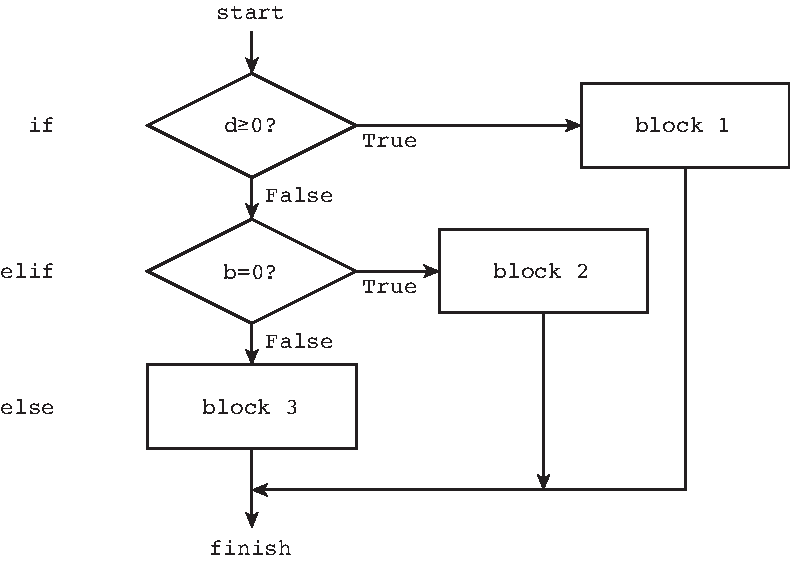
\includegraphics{flow_if_elif_else.pdf}}
\caption{Flowchart for \code{if}-\code{elif}-\code{else} code.}\label{chap6/chap6_loopsconds:fig-flow-if-elif-else}\end{figure}

At the outset of this problem we stated that the solutions to the quadratic equation are imaginary only if \(b=0\) and \(d < 0\).  In the \code{elif b == 0.0} statement on line 9, however, we only check to see if  \(b=0\).  The reason that we don't have to check if \(d < 0\) is that the \code{elif} statement is executed only if the condition \code{if d \textgreater{}= 0.0} on line 7 is \code{False}.  Similarly, we don't have to check if if \(b=0\) and \(d < 0\) for the final \code{else} statement because this part of the \code{if}, \code{elif}, and \code{else} block will only be executed if the preceding \code{if} and \code{elif} statements are \code{False}.  This illustrates a key feature of the \code{if}, \code{elif}, and \code{else} statements: these statements are executed sequentially until one of the \code{if} or \code{elif} statements is found to be \code{True}.  Therefore, Python reaches an \code{elif} or \code{else} statement only if all the preceding \code{if} and \code{elif} statements are \code{False}.

The \code{if}-\code{elif}-\code{else} logical structure can accomodate as many \code{elif} blocks as desired.  This allows you to set up logic with more than the three possible outcomes illustrated in the example above.  When designing the logical structure you should keep in mind that once Python finds a true condition, it skips all subsequent \code{elif} and \code{else} statements in a given \code{if}, \code{elif}, and \code{else} block, irrespective of their truth values.


\subsubsection{\texttt{if}-\texttt{else} example}
\label{chap6/chap6_loopsconds:if-else-example}
You will often run into situations where you simply want the program to execute one of two possible blocks based on the outcome of an \code{if} statement.  In this case, the \code{elif} block is omitted and you simply use an \code{if}-\code{else} structure.  The following program testing whether an integer is even or odd provides a simple example.

\begin{Verbatim}[commandchars=\\\{\}]
\PYG{g+go}{a = int(raw\PYGZus{}input(\PYGZdq{}Please input an integer: \PYGZdq{}))}
\PYG{g+go}{if a\PYGZpc{}2 == 0:}
\PYG{g+go}{    print(\PYGZdq{}\PYGZob{}0:0d\PYGZcb{} is an even number.\PYGZdq{}.format(a))}
\PYG{g+go}{else:}
\PYG{g+go}{    print(\PYGZdq{}\PYGZob{}0:0d\PYGZcb{} is an odd number.\PYGZdq{}.format(a))}
\end{Verbatim}

The flowchart below shows the logical structure of an \code{if}-\code{else} structure.
\begin{figure}[htbp]
\centering
\capstart

\scalebox{0.800000}{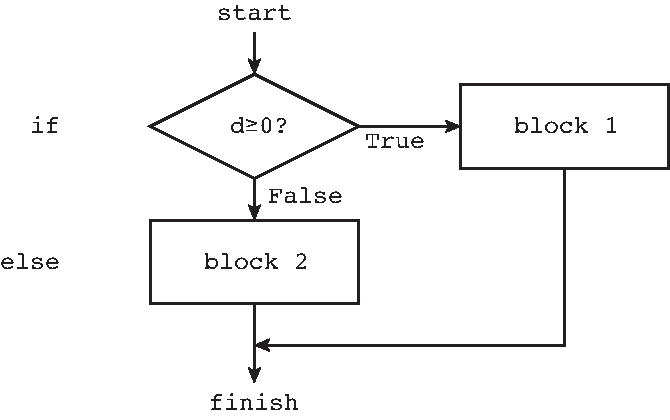
\includegraphics{flow_if_else.pdf}}
\caption{Flowchart for \code{if}-\code{else} code.}\label{chap6/chap6_loopsconds:fig-flow-if-else}\end{figure}


\subsubsection{\texttt{if} example}
\label{chap6/chap6_loopsconds:if-example}
The simplest logical structure you can make is a simple \code{if} statement, which executes a block of code if some condition is met but otherwise does nothing.  The program below, which takes the absolute value of a number, provides a simple example of such a case.

\begin{Verbatim}[commandchars=\\\{\}]
\PYG{g+go}{a = eval(raw\PYGZus{}input(\PYGZdq{}Please input a number: \PYGZdq{}))}
\PYG{g+go}{if a \PYGZlt{} 0:}
\PYG{g+go}{    a = \PYGZhy{}a}
\PYG{g+go}{print(\PYGZdq{}The absolute value is \PYGZob{}0\PYGZcb{}\PYGZdq{}.format(a))}
\end{Verbatim}

When the block of code in an \code{if} or \code{elif} statement is only one line long, you can write it on the same line as the \code{if} or \code{elif} statement.  For example, the above code can be written as follows.

\begin{Verbatim}[commandchars=\\\{\}]
\PYG{g+go}{a = eval(raw\PYGZus{}input(\PYGZdq{}Please input a number: \PYGZdq{}))}
\PYG{g+go}{if a \PYGZlt{} 0: a = \PYGZhy{}a}
\PYG{g+go}{print(\PYGZdq{}The absolute value is \PYGZob{}0\PYGZcb{}\PYGZdq{}.format(a))}
\end{Verbatim}

This works exactly as the preceding code.  Note, however, that if the block of code associated with an \code{if} or \code{elif} statement is more than one line long, the entire block of code should be written as indented text below the \code{if} or \code{elif} statement.

The flowchart below shows the logical structure of a simple \code{if} structure.
\begin{figure}[htbp]
\centering
\capstart

\scalebox{0.800000}{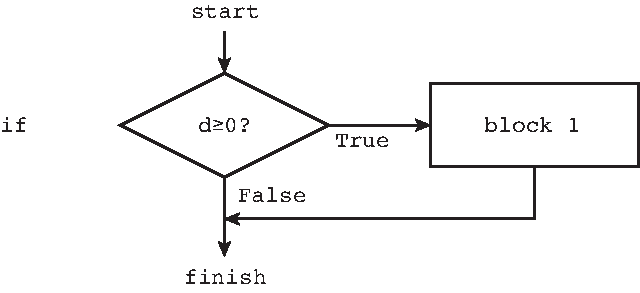
\includegraphics{flow_if.pdf}}
\caption{Flowchart for \code{if} code.}\label{chap6/chap6_loopsconds:fig-flow-if}\end{figure}

\index{logical operators}

\subsection{Logical operators}
\label{chap6/chap6_loopsconds:logical-operators}\label{chap6/chap6_loopsconds:index-1}
It is important to understand that ``\code{==}'' in Python is not the same as ``\code{=}''.  The operator ``\code{=}'' is the assignment operator: \code{d = 5} assigns the value of 5 to the valiable \code{d}.  On the other hand ``\code{==}'' is the \emph{logical equals operator} and \code{d == 5} is a \emph{logical truth statement}.  It tells Python to check to see if \code{d} is equal to \code{5} or not, and assigns a value of \code{True} or \code{False} to the statement \code{d == 5} depending on whether or not \code{d} is equal to \code{5}.  The table below summarizes the various logical operators available in Python.
\begin{quote}

\begin{tabulary}{\linewidth}{|L|L|}
\hline
\textsf{\relax 
operator
} & \textsf{\relax 
function
}\\
\hline
\textless{}
 & 
less than
\\

\textless{}=
 & 
less than or equal to
\\

\textgreater{}
 & 
greater than
\\

\textgreater{}=
 & 
greater than or equal to
\\

==
 & 
equal
\\

!=
 & 
not equal
\\

\code{and}
 & 
both must be true
\\

\code{or}
 & 
one or both must be true
\\

\code{not}
 & 
reverses the truth value
\\
\hline\end{tabulary}


Logical operators in Python
\end{quote}

The table above list three logical operators, \code{and}, \code{or}, and \code{not}, that we haven't encountered before.  There are useful for combining different logical conditions.  For example, suppose you want to check if \(a>2\) and \(b<10\) simultaneously.  To do so, you would write \code{a\textgreater{}2 and b\textless{}10}.  The code below illustrates the use of the logical operators \code{and}, \code{or}, and \code{not}.

\begin{Verbatim}[commandchars=\\\{\}]
\PYG{g+gp}{In [5]: }\PYG{n}{a} \PYG{o}{=} \PYG{l+m+mi}{5}

\PYG{g+gp}{In [6]: }\PYG{n}{b} \PYG{o}{=} \PYG{l+m+mi}{10}

\PYG{g+gp}{In [7]: }\PYG{n}{a} \PYG{o}{!=} \PYG{l+m+mi}{5}          \PYG{c}{\PYGZsh{} a is not equal to 5}
\PYG{g+gr}{Out[7]: }\PYG{n+nb+bp}{False}

\PYG{g+gp}{In [8]: }\PYG{n}{a}\PYG{o}{\PYGZgt{}}\PYG{l+m+mi}{2} \PYG{o+ow}{and} \PYG{n}{b}\PYG{o}{\PYGZlt{}}\PYG{l+m+mi}{20}
\PYG{g+gr}{Out[8]: }\PYG{n+nb+bp}{True}

\PYG{g+gp}{In [9]: }\PYG{n}{a}\PYG{o}{\PYGZgt{}}\PYG{l+m+mi}{2} \PYG{o+ow}{and} \PYG{n}{b}\PYG{o}{\PYGZgt{}}\PYG{l+m+mi}{10}
\PYG{g+gr}{Out[9]: }\PYG{n+nb+bp}{False}

\PYG{g+gp}{In [10]: }\PYG{n}{a}\PYG{o}{\PYGZgt{}}\PYG{l+m+mi}{2} \PYG{o+ow}{or} \PYG{n}{b}\PYG{o}{\PYGZgt{}}\PYG{l+m+mi}{10}
\PYG{g+gr}{Out[10]: }\PYG{n+nb+bp}{True}

\PYG{g+gp}{In [11]: }\PYG{n}{a}\PYG{o}{\PYGZgt{}}\PYG{l+m+mi}{2}
\PYG{g+gr}{Out[11]: }\PYG{n+nb+bp}{True}

\PYG{g+gp}{In [12]: }\PYG{o+ow}{not} \PYG{n}{a}\PYG{o}{\PYGZgt{}}\PYG{l+m+mi}{2}
\PYG{g+gr}{Out[12]: }\PYG{n+nb+bp}{False}
\end{Verbatim}

Logical statements like those above can be used in \code{if}, \code{elif}, and, as we shall see below, \code{while} statements, according to your needs.

\index{loops}

\section{Loops}
\label{chap6/chap6_loopsconds:loops}\label{chap6/chap6_loopsconds:index-2}
In computer programming a \emph{loop} is statement or block of statements that is executed repeatedly.  Python has two kinds of loops, a \code{for} loop and a \code{while} loop.  We first introduce the \code{for} loop and illustrate its use for a variety of tasks.  We then introduce the \code{while} loop and, after a few illustrative examples, compare the two kinds of loops and discuss when to use one or the other.

\index{loops!for loops}

\subsection{\texttt{for} loops}
\label{chap6/chap6_loopsconds:for-loops}\label{chap6/chap6_loopsconds:index-3}
The general form of a \code{for} loop in Python is

\begin{Verbatim}[commandchars=\\\{\}]
\PYG{k}{for} \PYG{o}{\PYGZlt{}}\PYG{n}{itervar}\PYG{o}{\PYGZgt{}} \PYG{o+ow}{in} \PYG{o}{\PYGZlt{}}\PYG{n}{sequence}\PYG{o}{\PYGZgt{}}\PYG{p}{:}
    \PYG{o}{\PYGZlt{}}\PYG{n}{body}\PYG{o}{\PYGZgt{}}
\end{Verbatim}

where \code{\textless{}intervar\textgreater{}} is a variable, \code{\textless{}sequence\textgreater{}} is a sequence such as list or string or array, and \code{\textless{}body\textgreater{}} is a series of Python commands to be executed repeatedly for each element in the \code{\textless{}sequence\textgreater{}}.  The \code{\textless{}body\textgreater{}} is indented from the rest of the text, which difines the extent of the loop.  Let's look at a few examples.

\begin{Verbatim}[commandchars=\\\{\}]
\PYG{k}{for} \PYG{n}{dogname} \PYG{o+ow}{in} \PYG{p}{[}\PYG{l+s}{\PYGZdq{}}\PYG{l+s}{Max}\PYG{l+s}{\PYGZdq{}}\PYG{p}{,} \PYG{l+s}{\PYGZdq{}}\PYG{l+s}{Molly}\PYG{l+s}{\PYGZdq{}}\PYG{p}{,} \PYG{l+s}{\PYGZdq{}}\PYG{l+s}{Buster}\PYG{l+s}{\PYGZdq{}}\PYG{p}{,} \PYG{l+s}{\PYGZdq{}}\PYG{l+s}{Maggie}\PYG{l+s}{\PYGZdq{}}\PYG{p}{,} \PYG{l+s}{\PYGZdq{}}\PYG{l+s}{Lucy}\PYG{l+s}{\PYGZdq{}}\PYG{p}{]}\PYG{p}{:}
    \PYG{k}{print}\PYG{p}{(}\PYG{n}{dogname}\PYG{p}{)}
    \PYG{k}{print}\PYG{p}{(}\PYG{l+s}{\PYGZdq{}}\PYG{l+s}{    Arf, arf!}\PYG{l+s}{\PYGZdq{}}\PYG{p}{)}
\PYG{k}{print}\PYG{p}{(}\PYG{l+s}{\PYGZdq{}}\PYG{l+s}{All done.}\PYG{l+s}{\PYGZdq{}}\PYG{p}{)}
\end{Verbatim}

Running this program produces the following output.

\begin{Verbatim}[commandchars=\\\{\}]
\PYG{g+gp}{In [1]: }\PYG{n}{run} \PYG{n}{doggyloop}\PYG{o}{.}\PYG{n}{py}
\PYG{g+go}{Max}
\PYG{g+go}{    Arf, arf!}
\PYG{g+go}{Molly}
\PYG{g+go}{    Arf, arf!}
\PYG{g+go}{Buster}
\PYG{g+go}{    Arf, arf!}
\PYG{g+go}{Maggie}
\PYG{g+go}{    Arf, arf!}
\PYG{g+go}{Lucy}
\PYG{g+go}{    Arf, arf!}
\PYG{g+go}{All done.}
\end{Verbatim}

The \code{for} loop works as follows: the \emph{iteration variable} or \emph{loop index} \code{dogname} is set equal to the first element in the list, \code{"Max"}, and then the two lines in the indented body are executed.  Then \code{dogname} is set equal to second element in the list, \code{"Molly"}, and the two lines in the indented body are executed.  The loop cycles through all the elements of the list, and then moves on to the code that follows the \code{for} loop and prints \code{All done.}

When indenting a block of code in a Python \code{for} loop, it is critical that every line be indented by the same amount.  Using the \textbf{\textless{}tab\textgreater{}} key causes the Code Editor to indent 4 spaces.  Any amount of indentation works, as long as it is the same for all lines in a \code{for} loop.  While code editors designed to work with Python (including Canopy and Spyder) translate the \textbf{\textless{}tab\textgreater{}} key to 4 spaces, not all text editors do.  In those cases, 4 spaces are not equivalent to a \textbf{\textless{}tab\textgreater{}} character even if they appear the same on the display.  Indenting some lines by 4 spaces and other lines by a \textbf{\textless{}tab\textgreater{}} character will produce an error.  So beware!

The figure below shows the flowchart for a \code{for} loop.  It starts with an implicit conditional asking if there are any more elements in the sequence.  If there are, it sets the iteration variable equal to the next element in the sequence and then executes the body---the indented text---using that value of the iteration variable.  It then  returns to the beginning to see if there are more elements in the sequence and continues the loop until there is none remaining.
\begin{figure}[htbp]
\centering
\capstart

\scalebox{0.800000}{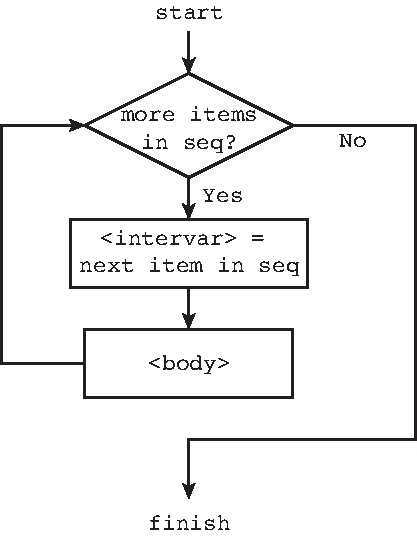
\includegraphics{flow_for.pdf}}
\caption{Flowchart for \code{for}-loop.}\label{chap6/chap6_loopsconds:fig-flow-for}\end{figure}


\subsection{Accumulators}
\label{chap6/chap6_loopsconds:accumulators}
Let's look at another application of Python's \code{for} loop.  Suppose you want to calculate the sum of all the odd numbers between 1 and 100.  Before writing a computer program to do this, let's think about how you would do it by hand.  You might start by adding 1+3=4.  Then take the result 4 and add the next odd integer, 5, to get 4+5=9; then 9+7=16, then 16+9=25, and so forth.  You are doing repeated additions, starting with 1+3, while keeping track of the running sum, until you reach the last number 99.

In developing an algorithm for having the computer sum the series of numbers, we are going to do the same thing: add the numbers one at a time while keeping track of the running sum, until we reach the last number.  We will keep track of the running sum with the variable \code{s}, which is called the \emph{accumulator}.  Initially \code{s=0}, since we haven't adding any numbers yet.  Then we add the first number, 1, to \code{s} and \code{s} becomes 1.  Then we add then next number, 3, in our sequence of odd numbers to \code{s} and \code{s} becomes 4.  We continue doing this over and over again using a \code{for} loop while the variable \code{s} accumulates the running sum until we reach the final number.  The code below illustrates how to do this.

\begin{Verbatim}[commandchars=\\\{\},numbers=left,firstnumber=1,stepnumber=1]
\PYG{n}{s} \PYG{o}{=} \PYG{l+m+mi}{0}
\PYG{k}{for} \PYG{n}{i} \PYG{o+ow}{in} \PYG{n+nb}{range}\PYG{p}{(}\PYG{l+m+mi}{1}\PYG{p}{,} \PYG{l+m+mi}{100}\PYG{p}{,} \PYG{l+m+mi}{2}\PYG{p}{)}\PYG{p}{:}
    \PYG{n}{s} \PYG{o}{=} \PYG{n}{s}\PYG{o}{+}\PYG{n}{i}
\PYG{k}{print}\PYG{p}{(}\PYG{n}{s}\PYG{p}{)}
\end{Verbatim}

The \code{range} function defines the list \code{{[}1, 3, 5, ..., 97, 99{]}}.  The \code{for} loop successively adds each number in the list to the running sum until it reaches the last element in the list and the sum is complete.  Once the \code{for} loop finishes, the program exits the loop and the final value of \code{s}, which is the sum of the odd numbers from 1 to 99, is printed out.  Copy the above program and run it.  You should get an answer of 2500.

\index{loops!while loops}

\subsection{\texttt{while} loops}
\label{chap6/chap6_loopsconds:index-4}\label{chap6/chap6_loopsconds:while-loops}
The general form of a \code{while} loop in Python is

\begin{Verbatim}[commandchars=\\\{\}]
\PYG{k}{while} \PYG{o}{\PYGZlt{}}\PYG{n}{condition}\PYG{o}{\PYGZgt{}}\PYG{p}{:}
    \PYG{o}{\PYGZlt{}}\PYG{n}{body}\PYG{o}{\PYGZgt{}}
\end{Verbatim}

where \code{\textless{}condition\textgreater{}} is a statement that can be either \code{True} or \code{False} and \code{\textless{}body\textgreater{}} is a series of Python commands that is executed repeatedly until \code{\textless{}condition\textgreater{}} becomes false.  This means that somewhere in \code{\textless{}body\textgreater{}}, the truth value of \textless{}condition\textgreater{} must be changed so that it becomes false after a finite number of iterations.  Consider the following example.

Suppose you want to calculate all the Fibonacci numbers smaller than 1000.  The Fibonacci numbers are determined by starting with the integers 0 and 1.  The next number in the sequence is the sum of the previous two.  So, starting with 0 and 1, the next Fibonacci number is \(0+1=1\), giving the sequence \(0, 1, 1\).  Continuing this process, we obtain \(0, 1, 1, 2, 3, 5, 8, ...\) where each element in the list is the sum of the previous two.   Using a \code{for} loop to calculate the Fibonacci numbers is impractical because we do not know ahead of time how many Fibonacci numbers there are smaller than 1000.  By contrast a \code{while} loop is perfect for calculating all the Fibonacci numbers because it keeps calculating Fibonacci numbers until it reaches the desired goal, in this case 1000.  Here is the code using a \code{while} loop.

\begin{Verbatim}[commandchars=\\\{\}]
\PYG{n}{x}\PYG{p}{,} \PYG{n}{y} \PYG{o}{=} \PYG{l+m+mi}{0}\PYG{p}{,} \PYG{l+m+mi}{1}
\PYG{k}{while} \PYG{n}{x} \PYG{o}{\PYGZlt{}} \PYG{l+m+mi}{1000}\PYG{p}{:}
    \PYG{k}{print}\PYG{p}{(}\PYG{n}{x}\PYG{p}{)}
    \PYG{n}{x}\PYG{p}{,} \PYG{n}{y} \PYG{o}{=} \PYG{n}{y}\PYG{p}{,} \PYG{n}{x}\PYG{o}{+}\PYG{n}{y}
\end{Verbatim}

We have used the multiple assignment feature of Python in this code.  Recall that all the values on the left are assigned using the original values of \code{x} and \code{y}.

The figure below shows the flowchart for the \code{while} loop.  The loop starts with the evaluation of a condition.  If the condition is \code{False}, the code in the body is skipped, the flow exits the loop, and then continues with the rest of the program.  If the condition is \code{True}, the code in the body---the indented text---is executed.  Once the body is finished, the flow returns to the condition and proceeds along the \code{True} or \code{False} branches depending on the truth value of the condition.  Implicit in this loop is the idea that somewhere during the execution of the body of the while loop, the variable that is evaluated in the condition is changed in some way.  Eventually that change will cause the condition to return a value of \code{False} so that the loop will end.
\begin{figure}[htbp]
\centering
\capstart

\scalebox{0.800000}{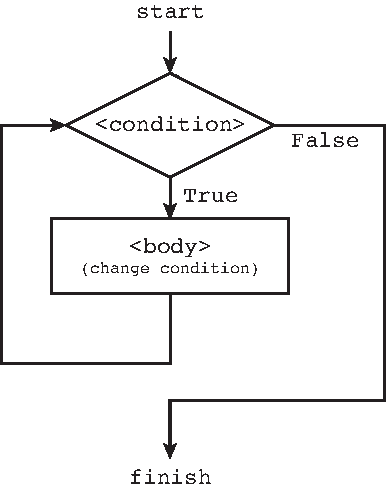
\includegraphics{flow_while.pdf}}
\caption{Flowchart for \code{while} loop.}\label{chap6/chap6_loopsconds:fig-flow-while}\end{figure}

One danger of a \code{while} loop is that it entirely possible to write a loop that never terminates---an \emph{infinite loop}.  For example, if we had written \code{while y \textgreater{} 0:}, in place of \code{while x \textless{} 1000:}, the loop would never end.  If you execute code that has an infinite loop, you can often terminate the program from the keyboard by typing \textbf{ctrl-C} a couple of times.  If that doesn't work, you may have to terminate and then restart Python.

For the kind of work we do in science and engineering, we generally find that the \code{for} loop is more useful than the \code{while} loop.  Nevertheless, there are times when using a \code{while} loop is better suited to a task than is a \code{for} loop.


\subsection{Loops and array operations}
\label{chap6/chap6_loopsconds:loops-and-array-operations}
Loops are often used to sequentially modify the elements of an array.  For example, suppose we want to square each element of the array \code{a = np.linspace(0, 32, 1e7)}.  This is a hefty array with 10 million elements.  Nevertheless, the following loop does the trick.

\begin{Verbatim}[commandchars=\\\{\}]
\PYG{k+kn}{import} \PYG{n+nn}{numpy} \PYG{k+kn}{as} \PYG{n+nn}{np}
\PYG{n}{a} \PYG{o}{=} \PYG{n}{np}\PYG{o}{.}\PYG{n}{linspace}\PYG{p}{(}\PYG{l+m+mi}{0}\PYG{p}{,} \PYG{l+m+mi}{32}\PYG{p}{,} \PYG{l+m+mf}{1e7}\PYG{p}{)}
\PYG{k}{print}\PYG{p}{(}\PYG{n}{a}\PYG{p}{)}
\PYG{k}{for} \PYG{n}{i} \PYG{o+ow}{in} \PYG{n+nb}{range}\PYG{p}{(}\PYG{n+nb}{len}\PYG{p}{(}\PYG{n}{a}\PYG{p}{)}\PYG{p}{)}\PYG{p}{:}
    \PYG{n}{a}\PYG{p}{[}\PYG{n}{i}\PYG{p}{]} \PYG{o}{=} \PYG{n}{a}\PYG{p}{[}\PYG{n}{i}\PYG{p}{]}\PYG{o}{*}\PYG{n}{a}\PYG{p}{[}\PYG{n}{i}\PYG{p}{]}
\PYG{k}{print}\PYG{p}{(}\PYG{n}{a}\PYG{p}{)}
\end{Verbatim}

Running this on my computer returns the result in about 8 seconds---not bad for having performed 10 million multiplications.  Of course we could have performed the same calculation using the array multiplication we learned in Chapter 3 ({\hyperref[chap3/chap3_arrays:chap3]{\emph{Strings, Lists, Arrays, and Dictionaries}}}).  Here is the code.

\begin{Verbatim}[commandchars=\\\{\}]
\PYG{k+kn}{import} \PYG{n+nn}{numpy} \PYG{k+kn}{as} \PYG{n+nn}{np}
\PYG{n}{a} \PYG{o}{=} \PYG{n}{np}\PYG{o}{.}\PYG{n}{linspace}\PYG{p}{(}\PYG{l+m+mi}{0}\PYG{p}{,} \PYG{l+m+mi}{32}\PYG{p}{,} \PYG{l+m+mf}{1e7}\PYG{p}{)}
\PYG{k}{print}\PYG{p}{(}\PYG{n}{a}\PYG{p}{)}
\PYG{n}{a} \PYG{o}{=} \PYG{n}{a}\PYG{o}{*}\PYG{n}{a}
\PYG{k}{print}\PYG{p}{(}\PYG{n}{a}\PYG{p}{)}
\end{Verbatim}

Running this on my computer returns the results faster than I can discern, but certainly much less than a second.  This illustrates an important point: \textbf{for loops are slow}.  Array operations run much faster and are therefore to be preferred in any case where you have a choice.  Sometimes finding an array operation that is equivalent to a loop can be difficult, especially for a novice.  Nevertheless, doing so pays rich rewards in execution time.  Moreover, the array notation is usually simpler and clearer, providing further reasons to prefer array operations over loops.

\index{list comprehension}

\section{List Comprehensions}
\label{chap6/chap6_loopsconds:index-5}\label{chap6/chap6_loopsconds:list-comprehensions}
List comprehensions are a special feature of core Python for processing and constructing lists.  We introduce them here because they use a looping process.  They are used quite commonly in Python coding and they often provide elegant compact solutions to some common computing tasks.

Consider, for example the \(3 \times 3\) matrix

\begin{Verbatim}[commandchars=\\\{\}]
\PYG{g+gp}{In [1]: }\PYG{n}{x} \PYG{o}{=} \PYG{p}{[}\PYG{p}{[}\PYG{l+m+mi}{1}\PYG{p}{,} \PYG{l+m+mi}{2}\PYG{p}{,} \PYG{l+m+mi}{3}\PYG{p}{]}\PYG{p}{,} \PYG{p}{[}\PYG{l+m+mi}{4}\PYG{p}{,} \PYG{l+m+mi}{5}\PYG{p}{,} \PYG{l+m+mi}{6}\PYG{p}{]}\PYG{p}{,} \PYG{p}{[}\PYG{l+m+mi}{7}\PYG{p}{,} \PYG{l+m+mi}{8}\PYG{p}{,} \PYG{l+m+mi}{9}\PYG{p}{]}\PYG{p}{]}
\end{Verbatim}

Suppose we want to construct a vector from the diagonal elements of this matrix.  We could do so with a \code{for} loop with an accumulator as follows

\begin{Verbatim}[commandchars=\\\{\}]
\PYG{g+gp}{In [2]: }\PYG{n}{diag} \PYG{o}{=} \PYG{p}{[}\PYG{p}{]}
\PYG{g+gp}{   ...:} \PYG{k}{for} \PYG{n}{i} \PYG{o+ow}{in} \PYG{p}{[}\PYG{l+m+mi}{0}\PYG{p}{,} \PYG{l+m+mi}{1}\PYG{p}{,} \PYG{l+m+mi}{2}\PYG{p}{]}\PYG{p}{:}
\PYG{g+gp}{   ...:}     \PYG{n}{diag}\PYG{o}{.}\PYG{n}{append}\PYG{p}{(}\PYG{n}{x}\PYG{p}{[}\PYG{n}{i}\PYG{p}{]}\PYG{p}{[}\PYG{n}{i}\PYG{p}{]}\PYG{p}{)}
\PYG{g+gp}{   ...:}

\PYG{g+gp}{In [3]: }\PYG{n}{diag}
\PYG{g+gr}{Out[3]: }\PYG{p}{[}\PYG{l+m+mi}{1}\PYG{p}{,} \PYG{l+m+mi}{5}\PYG{p}{,} \PYG{l+m+mi}{9}\PYG{p}{]}
\end{Verbatim}

List comprehensions provide a simpler, cleaner, and faster way of doing the same thing

\begin{Verbatim}[commandchars=\\\{\}]
\PYG{g+gp}{In [4]: }\PYG{n}{diagLC} \PYG{o}{=} \PYG{p}{[}\PYG{n}{x}\PYG{p}{[}\PYG{n}{i}\PYG{p}{]}\PYG{p}{[}\PYG{n}{i}\PYG{p}{]} \PYG{k}{for} \PYG{n}{i} \PYG{o+ow}{in} \PYG{p}{[}\PYG{l+m+mi}{0}\PYG{p}{,} \PYG{l+m+mi}{1}\PYG{p}{,} \PYG{l+m+mi}{2}\PYG{p}{]}\PYG{p}{]}

\PYG{g+gp}{In [5]: }\PYG{n}{diagLC}
\PYG{g+gr}{Out[5]: }\PYG{p}{[}\PYG{l+m+mi}{1}\PYG{p}{,} \PYG{l+m+mi}{5}\PYG{p}{,} \PYG{l+m+mi}{9}\PYG{p}{]}
\end{Verbatim}

A one-line list comprehension replaces a three-line accumulator plus loop code.

Suppose we now want the square of this list:

\begin{Verbatim}[commandchars=\\\{\}]
\PYG{g+gp}{In [6]: }\PYG{p}{[}\PYG{n}{y}\PYG{o}{*}\PYG{n}{y} \PYG{k}{for} \PYG{n}{y} \PYG{o+ow}{in} \PYG{n}{diagLC}\PYG{p}{]}
\PYG{g+gr}{Out[6]: }\PYG{p}{[}\PYG{l+m+mi}{1}\PYG{p}{,} \PYG{l+m+mi}{25}\PYG{p}{,} \PYG{l+m+mi}{81}\PYG{p}{]}
\end{Verbatim}

Notice here how \code{y} serves as a dummy variable accessing the various elements of the list \code{diagLC}.

Extracting a column from a 2-dimensaional array such as \code{x} is quite easy.   For example the second row is obtained quite simply in the following fashion

\begin{Verbatim}[commandchars=\\\{\}]
\PYG{g+gp}{In [7]: }\PYG{n}{x}\PYG{p}{[}\PYG{l+m+mi}{1}\PYG{p}{]}
\PYG{g+gr}{Out[7]: }\PYG{p}{[}\PYG{l+m+mi}{4}\PYG{p}{,} \PYG{l+m+mi}{5}\PYG{p}{,} \PYG{l+m+mi}{6}\PYG{p}{]}
\end{Verbatim}

Obtaining a column is not as simple, but a list comprehension makes it quite straightforward:

\begin{Verbatim}[commandchars=\\\{\}]
\PYG{g+gp}{In [7]: }\PYG{n}{c1} \PYG{o}{=} \PYG{p}{[}\PYG{n}{a}\PYG{p}{[}\PYG{l+m+mi}{1}\PYG{p}{]} \PYG{k}{for} \PYG{n}{a} \PYG{o+ow}{in} \PYG{n}{x}\PYG{p}{]}
\PYG{g+gp}{In [8]: }\PYG{n}{c1}
\PYG{g+gr}{Out[8]: }\PYG{p}{[}\PYG{l+m+mi}{2}\PYG{p}{,} \PYG{l+m+mi}{5}\PYG{p}{,} \PYG{l+m+mi}{8}\PYG{p}{]}
\end{Verbatim}

Another, slightly less elegant way to accomplish the same thing is

\begin{Verbatim}[commandchars=\\\{\}]
\PYG{g+gp}{In [9]: }\PYG{p}{[}\PYG{n}{x}\PYG{p}{[}\PYG{n}{i}\PYG{p}{]}\PYG{p}{[}\PYG{l+m+mi}{1}\PYG{p}{]} \PYG{k}{for} \PYG{n}{i} \PYG{o+ow}{in} \PYG{n+nb}{range}\PYG{p}{(}\PYG{l+m+mi}{3}\PYG{p}{)}\PYG{p}{]}
\PYG{g+gr}{Out[9]: }\PYG{p}{[}\PYG{l+m+mi}{2}\PYG{p}{,} \PYG{l+m+mi}{5}\PYG{p}{,} \PYG{l+m+mi}{8}\PYG{p}{]}
\end{Verbatim}

Suppose you have a list of numbers and you want to extract all the elements of the list that are divisible by three.  A slightly fancier list comprehension accomplishes the task quite simply and demonstrates a new feature:

\begin{Verbatim}[commandchars=\\\{\}]
\PYG{g+gp}{In [10]: } \PYG{n}{y} \PYG{o}{=} \PYG{p}{[}\PYG{o}{\PYGZhy{}}\PYG{l+m+mi}{5}\PYG{p}{,} \PYG{o}{\PYGZhy{}}\PYG{l+m+mi}{3}\PYG{p}{,} \PYG{l+m+mi}{1}\PYG{p}{,} \PYG{l+m+mi}{7}\PYG{p}{,} \PYG{l+m+mi}{4}\PYG{p}{,} \PYG{l+m+mi}{23}\PYG{p}{,} \PYG{l+m+mi}{27}\PYG{p}{,} \PYG{o}{\PYGZhy{}}\PYG{l+m+mi}{9}\PYG{p}{,} \PYG{l+m+mi}{11}\PYG{p}{,} \PYG{l+m+mi}{41}\PYG{p}{]}
\PYG{g+gp}{In [14]: }\PYG{p}{[}\PYG{n}{a} \PYG{k}{for} \PYG{n}{a} \PYG{o+ow}{in} \PYG{n}{y} \PYG{k}{if} \PYG{n}{a}\PYG{o}{\PYGZpc{}}\PYG{l+m+mi}{3}\PYG{o}{==}\PYG{l+m+mi}{0}\PYG{p}{]}
\PYG{g+gr}{Out[14]: }\PYG{p}{[}\PYG{o}{\PYGZhy{}}\PYG{l+m+mi}{3}\PYG{p}{,} \PYG{l+m+mi}{27}\PYG{p}{,} \PYG{o}{\PYGZhy{}}\PYG{l+m+mi}{9}\PYG{p}{]}
\end{Verbatim}

As we see in this example, a conditional statement can be added to a list comprehension.  Here it serves as a filter to select out only those elements that are divisible by three.
\newpage

\section{Exercises}
\label{chap6/chap6_loopsconds:exercises}\begin{enumerate}
\item {} 
Write a program to calculate the factorial of a positive integer input by the user.  Recall that the factorial function is given by \(x! = x (x-1) (x-2) ... (2) (1)\) so that \(1!=1\), \(2!=2\), \(3!=6\), \(4!=24\), ...
\begin{enumerate}
\item {} 
Write the factorial function using a Python \code{while} loop.

\item {} 
Write the factorial function using a Python \code{for} loop.

\end{enumerate}

Check your programs to make sure they work for 1, 2, 3, 5, and beyond, but especially for the first 5 integers.

\item {} 
The following Python program finds the smallest non-trivial (not 1) prime factor of a positive integer.

\begin{Verbatim}[commandchars=\\\{\}]
\PYG{n}{n} \PYG{o}{=} \PYG{n+nb}{int}\PYG{p}{(}\PYG{n+nb}{raw\PYGZus{}input}\PYG{p}{(}\PYG{l+s}{\PYGZdq{}}\PYG{l+s}{Input an integer \PYGZgt{} 1: }\PYG{l+s}{\PYGZdq{}}\PYG{p}{)}\PYG{p}{)}
\PYG{n}{i} \PYG{o}{=} \PYG{l+m+mi}{2}

\PYG{k}{while} \PYG{p}{(}\PYG{n}{n} \PYG{o}{\PYGZpc{}} \PYG{n}{i}\PYG{p}{)} \PYG{o}{!=} \PYG{l+m+mi}{0}\PYG{p}{:}
    \PYG{n}{i} \PYG{o}{+}\PYG{o}{=} \PYG{l+m+mi}{1}

\PYG{k}{print}\PYG{p}{(}\PYG{l+s}{\PYGZdq{}}\PYG{l+s}{The smallest factor of n is:}\PYG{l+s}{\PYGZdq{}}\PYG{p}{,} \PYG{n}{i} \PYG{p}{)}
\end{Verbatim}
\begin{enumerate}
\item {} 
Type this program into your computer and verify that it works as advertised.  Then briefly explain how it works and why the while loop always terminates.

\item {} 
Modify the program so that it tells you if the integer input is a prime number or not.  If it is not a prime number, write your program so that it prints out the smallest prime factor.  Using your program verify that the following integers are prime numbers: 101, 8191, 947431.

\end{enumerate}

\item {} 
Consider the matrix list \code{x = {[}{[}1, 2, 3{]}, {[}4, 5, 6{]}, {[}7, 8, 9{]}{]}}.  Write a list comprehension to extract the last column of the matrix {[}3, 6, 9{]}.  Write another list comprehension to create a vector of twice the square of the middle column \code{{[}8, 50, 128{]}}.

\item {} 
Write a program that calculates the value of an investment after some number of years specified by the user if
\begin{enumerate}
\item {} 
the principal is compounded annually

\item {} 
the principle is compounded monthly

\item {} 
the principle is compounded daily

\end{enumerate}

Your program should ask the user for the initial investment (principal), the interest rate in percent, and the number of years the money will be invested (allow for fractional years).  For an initial investment of \$1000 at an interest rate of 6\%, after 10 years I get \$1790.85 when compounded annually, \$1819.40 when compounded monthly, and \$1822.03 when compounded daily, assuming 12 months in a year and 365.24 days in a year, where the monthly interest rate is the annual rate divided by 12 and the daily rate is the annual rate divided by 365 (don't worry about leap years).

\item {} 
Write a program that determines the day of the week for any given calendar date after January 1, 1900, which was a Monday.  Your program will need to take into account leap years, which occur in every year that is divisible by 4, except for years that are divisible by 100 but are not divisible by 400.  For example, 1900 was not a leap year, but 2000 was a leap year.  Test that your program gives the following answers: Monday 1900 January 1, Tuesday 1933 December 5, Wednesday 1993 June 23, Thursday 1953 January 15, Friday 1963 November 22, Saturday 1919 June 28, Sunday 2005 August 28.

\end{enumerate}


\chapter{Functions}
\label{chap7/chap7_funcs:chap7}\label{chap7/chap7_funcs:functions}\label{chap7/chap7_funcs::doc}
As you develop more complex computer code, it becomes increasingly important to organize your code into modular blocks.  One important means for doing so is  \emph{user-defined} Python functions.  User-defined functions are a lot like built-in functions that we have encountered in core Python as well as in NumPy and Matplotlib.  The main difference is that user-defined functions are written by you.  The idea is to define functions to simplify your code and to allow you to reuse the same code in different contexts.

The number of ways that functions are used in programming is so varied that we cannot possibly enumerate all the possibilities.  As our use of Python functions in scientific program is somewhat specialized, we introduce only a few of the possible uses of Python functions, ones that are the most common in scientific programming.

\index{functions!user defined}

\section{User-defined functions}
\label{chap7/chap7_funcs:userdefdfuncs}\label{chap7/chap7_funcs:user-defined-functions}\label{chap7/chap7_funcs:index-0}
The NumPy package contains a plethora of mathematical functions.  You can find a listing of the mathematical functions available through NumPy on the web page \href{http://docs.scipy.org/doc/numpy/reference/routines.math.html}{http://docs.scipy.org/doc/numpy/reference/routines.math.html}.  While the list may seem pretty exhaustive, you may nevertheless find that you need a function that is not available in the NumPy Python library.  In those cases, you will want to write your own function.

In studies of optics and signal processing one often runs into the sinc function, which is defined as
\begin{gather}
\begin{split}\mathrm{sinc}\,x \equiv \frac{\sin x}{x} \;.\end{split}\notag
\end{gather}
Let's write a Python function for the sinc function.  Here is our first attempt:

\begin{Verbatim}[commandchars=\\\{\}]
\PYG{k}{def} \PYG{n+nf}{sinc}\PYG{p}{(}\PYG{n}{x}\PYG{p}{)}\PYG{p}{:}
    \PYG{n}{y} \PYG{o}{=} \PYG{n}{np}\PYG{o}{.}\PYG{n}{sin}\PYG{p}{(}\PYG{n}{x}\PYG{p}{)}\PYG{o}{/}\PYG{n}{x}
    \PYG{k}{return} \PYG{n}{y}
\end{Verbatim}

Every function definition begins with the word \code{def} followed by the name you want to give to the function, \code{sinc} in this case, then a list of arguments enclosed in parentheses, and finally terminated with a colon.  In this case there is only one argument, \code{x}, but in general there can be as many arguments as you want, including no arguments at all.  For the moment, we will consider just the case of a single argument.

The indented block of code following the first line defines what the function does.  In this case, the first line calculates \(\mathrm{sinc}\,x = \sin x/x\) and sets it equal to \code{y}.  The \code{return} statement of the last line tells Python to return the value of \code{y} to the user.

We can try it out in the IPython shell.  First we type in the function definition.

\begin{Verbatim}[commandchars=\\\{\}]
\PYG{g+gp}{In [1]: }\PYG{k}{def} \PYG{n+nf}{sinc}\PYG{p}{(}\PYG{n}{x}\PYG{p}{)}\PYG{p}{:}
\PYG{g+gp}{   ...:}     \PYG{n}{y} \PYG{o}{=} \PYG{n}{sin}\PYG{p}{(}\PYG{n}{x}\PYG{p}{)}\PYG{o}{/}\PYG{n}{x}
\PYG{g+gp}{   ...:}     \PYG{k}{return} \PYG{n}{y}
\end{Verbatim}

Because we are doing this from the IPython shell, we don't need to import NumPy; it's preloaded.  Now the function \(\mathrm{sinc}\,x\) is available to be used from the IPython shell

\begin{Verbatim}[commandchars=\\\{\}]
\PYG{g+gp}{In [2]: }\PYG{n}{sinc}\PYG{p}{(}\PYG{l+m+mi}{4}\PYG{p}{)}
\PYG{g+gr}{Out[2]: }\PYG{o}{\PYGZhy{}}\PYG{l+m+mf}{0.18920062382698205}

\PYG{g+gp}{In [3]: }\PYG{n}{a} \PYG{o}{=} \PYG{n}{sinc}\PYG{p}{(}\PYG{l+m+mf}{1.2}\PYG{p}{)}

\PYG{g+gp}{In [4]: }\PYG{n}{a}
\PYG{g+gr}{Out[4]: }\PYG{l+m+mf}{0.77669923830602194}

\PYG{g+gp}{In [5]: }\PYG{n}{sin}\PYG{p}{(}\PYG{l+m+mf}{1.2}\PYG{p}{)}\PYG{o}{/}\PYG{l+m+mf}{1.2}
\PYG{g+gr}{Out[5]: }\PYG{l+m+mf}{0.77669923830602194}
\end{Verbatim}

Inputs and outputs 4 and 5 verify that the function does indeed give the same result as an explicit calculation of \(\sin x/x\).

You may have noticed that there is a problem with our definition of \(\mathrm{sinc}\,x\) when \code{x=0.0}.  Let's try it out and see what happens

\begin{Verbatim}[commandchars=\\\{\}]
\PYG{g+gp}{In [6]: }\PYG{n}{sinc}\PYG{p}{(}\PYG{l+m+mf}{0.0}\PYG{p}{)}
\PYG{g+gr}{Out[6]: }\PYG{n}{nan}
\end{Verbatim}

IPython returns \code{nan} or ``not a number'', which occurs when Python attempts a division by zero, which is not defined.  This is not the desired response as \(\mathrm{sinc}\,x\) is, in fact, perfectly well defined for \(x=0\).  You can verify this using L'Hopital's rule, which you may have learned in your study of calculus, or you can ascertain the correct answer by calculating the Taylor series for \(\mathrm{sinc}\,x\).  Here is what we get
\begin{gather}
\begin{split}\mathrm{sinc}\,x = \frac{\sin x}{x}
                = \frac{x - \frac{x^3}{3!} + \frac{x^5}{5!} + ...}{x}
                = 1 - \frac{x^2}{3!} + \frac{x^4}{5!} + ... \;.\end{split}\notag
\end{gather}
From the Taylor series, it is clear that \(\mathrm{sinc}\,x\) is well-defined at and near \(x=0\) and that, in fact,  \(\mathrm{sinc}(0)=1\).  Let's modify our function so that it gives the correct value for \code{x=0}.

\begin{Verbatim}[commandchars=\\\{\}]
\PYG{g+gp}{In [7]: }\PYG{k}{def} \PYG{n+nf}{sinc}\PYG{p}{(}\PYG{n}{x}\PYG{p}{)}\PYG{p}{:}
\PYG{g+gp}{   ...:}     \PYG{k}{if} \PYG{n}{x}\PYG{o}{==}\PYG{l+m+mf}{0.0}\PYG{p}{:}
\PYG{g+gp}{   ...:}         \PYG{n}{y} \PYG{o}{=} \PYG{l+m+mf}{1.0}
\PYG{g+gp}{   ...:}     \PYG{k}{else}\PYG{p}{:}
\PYG{g+gp}{   ...:}         \PYG{n}{y} \PYG{o}{=} \PYG{n}{sin}\PYG{p}{(}\PYG{n}{x}\PYG{p}{)}\PYG{o}{/}\PYG{n}{x}
\PYG{g+gp}{   ...:}     \PYG{k}{return} \PYG{n}{y}

\PYG{g+gp}{In [8]: }\PYG{n}{sinc}\PYG{p}{(}\PYG{l+m+mi}{0}\PYG{p}{)}
\PYG{g+gr}{Out[8]: }\PYG{l+m+mf}{1.0}

\PYG{g+gp}{In [9]: }\PYG{n}{sinc}\PYG{p}{(}\PYG{l+m+mf}{1.2}\PYG{p}{)}
\PYG{g+gr}{Out[9]: }\PYG{l+m+mf}{0.77669923830602194}
\end{Verbatim}

Now our function gives the correct value for \code{x=0} as well as for values different from zero.

\index{functions!looping over arrays}

\subsection{Looping over arrays in user-defined functions}
\label{chap7/chap7_funcs:index-1}\label{chap7/chap7_funcs:loopingarrays}\label{chap7/chap7_funcs:looping-over-arrays-in-user-defined-functions}
The code for \(\mathrm{sinc}\,x\) works just fine when the argument is a single number or a variable that represents a single number.  However, if the argument is a NumPy array, we run into a problem, as illustrated below.

\begin{Verbatim}[commandchars=\\\{\}]
\PYG{g+gp}{In [10]: }\PYG{n}{x} \PYG{o}{=} \PYG{n}{arange}\PYG{p}{(}\PYG{l+m+mi}{0}\PYG{p}{,} \PYG{l+m+mf}{5.}\PYG{p}{,} \PYG{l+m+mf}{0.5}\PYG{p}{)}

\PYG{g+gp}{In [11]: }\PYG{n}{x}
\PYG{g+gr}{Out[11]: }\PYG{n}{array}\PYG{p}{(}\PYG{p}{[} \PYG{l+m+mf}{0.} \PYG{p}{,}  \PYG{l+m+mf}{0.5}\PYG{p}{,}  \PYG{l+m+mf}{1.} \PYG{p}{,}  \PYG{l+m+mf}{1.5}\PYG{p}{,}  \PYG{l+m+mf}{2.} \PYG{p}{,}  \PYG{l+m+mf}{2.5}\PYG{p}{,}  \PYG{l+m+mf}{3.} \PYG{p}{,}  \PYG{l+m+mf}{3.5}\PYG{p}{,}
\PYG{g+go}{                 4. ,  4.5])}

\PYG{g+gp}{In [12]: }\PYG{n}{sinc}\PYG{p}{(}\PYG{n}{x}\PYG{p}{)}
\PYG{g+go}{\PYGZhy{}\PYGZhy{}\PYGZhy{}\PYGZhy{}\PYGZhy{}\PYGZhy{}\PYGZhy{}\PYGZhy{}\PYGZhy{}\PYGZhy{}\PYGZhy{}\PYGZhy{}\PYGZhy{}\PYGZhy{}\PYGZhy{}\PYGZhy{}\PYGZhy{}\PYGZhy{}\PYGZhy{}\PYGZhy{}\PYGZhy{}\PYGZhy{}\PYGZhy{}\PYGZhy{}\PYGZhy{}\PYGZhy{}\PYGZhy{}\PYGZhy{}\PYGZhy{}\PYGZhy{}\PYGZhy{}\PYGZhy{}\PYGZhy{}\PYGZhy{}\PYGZhy{}\PYGZhy{}\PYGZhy{}\PYGZhy{}\PYGZhy{}\PYGZhy{}\PYGZhy{}\PYGZhy{}\PYGZhy{}\PYGZhy{}\PYGZhy{}\PYGZhy{}\PYGZhy{}\PYGZhy{}\PYGZhy{}\PYGZhy{}\PYGZhy{}\PYGZhy{}\PYGZhy{}\PYGZhy{}\PYGZhy{}\PYGZhy{}\PYGZhy{}\PYGZhy{}}
\PYG{g+go}{ValueError               Traceback (most recent call last)}
\PYG{g+go}{\PYGZhy{}\PYGZhy{}\PYGZhy{}\PYGZhy{}\PYGZgt{} 1 sinc(x)}

\PYG{g+go}{      1 def sinc(x):}
\PYG{g+go}{\PYGZhy{}\PYGZhy{}\PYGZhy{}\PYGZhy{}\PYGZgt{} 2     if x==0.0:}
\PYG{g+go}{      3         y = 1.0}
\PYG{g+go}{      4     else:}
\PYG{g+go}{      5         y = np.sin(x)/x}

\PYG{g+go}{ValueError: The truth value of an array with more than one}
\PYG{g+go}{            element is ambiguous.}
\end{Verbatim}

The \code{if} statement in Python is set up to evaluate the truth value of a single variable, not of multielement arrays.  When Python is asked to evaluate the truth value for a multi-element array, it doesn't know what to do and therefore returns an error.

An obvious way to handle this problem is to write the code so that it processes the array one element at a time, which you could do using a \code{for} loop, as illustrated below.

\begin{Verbatim}[commandchars=\\\{\},numbers=left,firstnumber=1,stepnumber=1]
\PYG{k}{def} \PYG{n+nf}{sinc}\PYG{p}{(}\PYG{n}{x}\PYG{p}{)}\PYG{p}{:}
    \PYG{n}{y} \PYG{o}{=} \PYG{p}{[}\PYG{p}{]}              \PYG{c}{\PYGZsh{} creates an empty list to store results}
    \PYG{k}{for} \PYG{n}{xx} \PYG{o+ow}{in} \PYG{n}{x}\PYG{p}{:}        \PYG{c}{\PYGZsh{} loops over all elements in x array}
        \PYG{k}{if} \PYG{n}{xx}\PYG{o}{==}\PYG{l+m+mf}{0.0}\PYG{p}{:}     \PYG{c}{\PYGZsh{} adds result of 1.0 to y list if}
            \PYG{n}{y} \PYG{o}{+}\PYG{o}{=} \PYG{p}{[}\PYG{l+m+mf}{1.0}\PYG{p}{]}  \PYG{c}{\PYGZsh{} xx is zero}
        \PYG{k}{else}\PYG{p}{:}           \PYG{c}{\PYGZsh{} adds result of sin(xx)/xx to y list if}
            \PYG{n}{y} \PYG{o}{+}\PYG{o}{=} \PYG{p}{[}\PYG{n}{np}\PYG{o}{.}\PYG{n}{sin}\PYG{p}{(}\PYG{n}{xx}\PYG{p}{)}\PYG{o}{/}\PYG{n}{xx}\PYG{p}{]}  \PYG{c}{\PYGZsh{} xx is not zero}
    \PYG{k}{return} \PYG{n}{np}\PYG{o}{.}\PYG{n}{array}\PYG{p}{(}\PYG{n}{y}\PYG{p}{)}  \PYG{c}{\PYGZsh{} converts y to array and returns array}

\PYG{k+kn}{import} \PYG{n+nn}{numpy} \PYG{k+kn}{as} \PYG{n+nn}{np}
\PYG{k+kn}{import} \PYG{n+nn}{matplotlib.pyplot} \PYG{k+kn}{as} \PYG{n+nn}{plt}

\PYG{n}{x} \PYG{o}{=} \PYG{n}{np}\PYG{o}{.}\PYG{n}{linspace}\PYG{p}{(}\PYG{o}{\PYGZhy{}}\PYG{l+m+mi}{10}\PYG{p}{,} \PYG{l+m+mi}{10}\PYG{p}{,} \PYG{l+m+mi}{256}\PYG{p}{)}
\PYG{n}{y} \PYG{o}{=} \PYG{n}{sinc}\PYG{p}{(}\PYG{n}{x}\PYG{p}{)}

\PYG{n}{plt}\PYG{o}{.}\PYG{n}{plot}\PYG{p}{(}\PYG{n}{x}\PYG{p}{,} \PYG{n}{y}\PYG{p}{)}
\PYG{n}{plt}\PYG{o}{.}\PYG{n}{axhline}\PYG{p}{(}\PYG{n}{color}\PYG{o}{=}\PYG{l+s}{\PYGZdq{}}\PYG{l+s}{gray}\PYG{l+s}{\PYGZdq{}}\PYG{p}{,} \PYG{n}{zorder}\PYG{o}{=}\PYG{o}{\PYGZhy{}}\PYG{l+m+mi}{1}\PYG{p}{)}
\PYG{n}{plt}\PYG{o}{.}\PYG{n}{axvline}\PYG{p}{(}\PYG{n}{color}\PYG{o}{=}\PYG{l+s}{\PYGZdq{}}\PYG{l+s}{gray}\PYG{l+s}{\PYGZdq{}}\PYG{p}{,} \PYG{n}{zorder}\PYG{o}{=}\PYG{o}{\PYGZhy{}}\PYG{l+m+mi}{1}\PYG{p}{)}
\PYG{n}{plt}\PYG{o}{.}\PYG{n}{show}\PYG{p}{(}\PYG{p}{)}
\end{Verbatim}

The \code{for} loop evaluates the elements of the \code{x} array one by one and appends the results to the list \code{y} one by one.  When it is finished, it converts the list to an array and returns the array.  The code following the function definition plots \(\mathrm{sinc}\,x\) as a function of \(x\).

In the program above, you may have noticed that the NumPy library is imported \emph{after} the \code{sinc(x)} function definition.  As the function uses the NumPy functions \code{sin} and \code{array}, you may wonder how this program can work.  Doesn't the \code{import numpy} statement have to be called before any NumPy functions are used?  The answer it an emphatic ``YES''.  What you need to understand is that the function definition is \emph{not executed} when it is defined, nor can it be as it has no input \code{x} data to process.  That part of the code is just a definition.  The first time the code for the \code{sinc(x)} function is actually executed is when it is called on line 14 of the program, which occurs after the NumPy library is imported in line 10.  The figure below shows the plot of the \(\mathrm{sinc}\,x\) function generated by the above code.
\begin{figure}[htbp]
\centering
\capstart

\scalebox{0.800000}{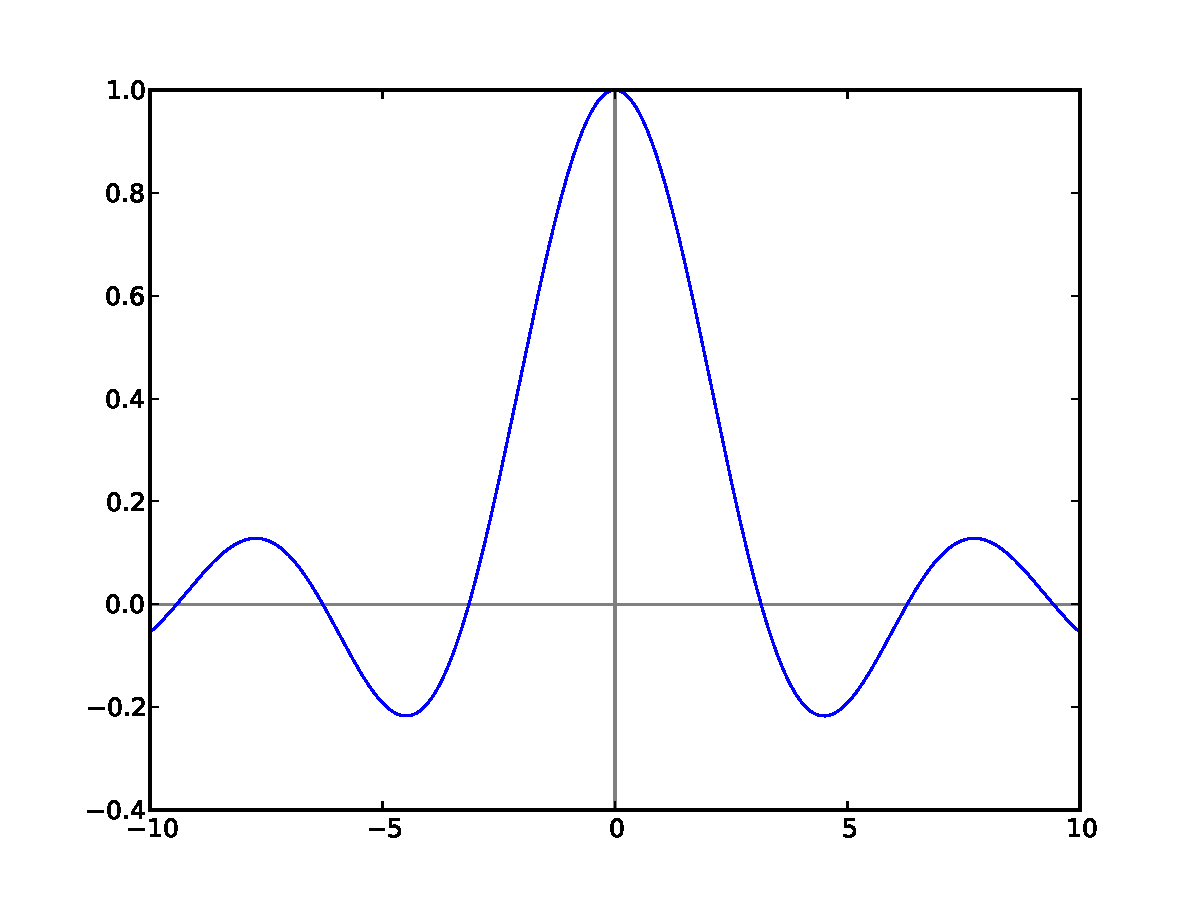
\includegraphics{sinc.pdf}}
\caption{Plot of user-defined \code{sinc(x)} function.}\end{figure}

\index{functions!fast array processing}\index{conditionals!applied to arrays}

\subsection{Fast array processing in user-defined functions}
\label{chap7/chap7_funcs:fast-array-processing-in-user-defined-functions}\label{chap7/chap7_funcs:index-2}
While using loops to process arrays works just fine, it is usually not the best way to accomplish the task in Python.  The reason is that loops in Python are executed rather slowly.  To deal with this problem, the developers of NumPy introduced a number of functions designed to process arrays quickly and efficiently.  For the present case, what we need is a conditional statement or function that can process arrays directly.  The function we want is called \code{where} and it is a part of the NumPy library.  There \code{where} function has the form

\begin{Verbatim}[commandchars=\\\{\}]
\PYG{n}{where}\PYG{p}{(}\PYG{n}{condition}\PYG{p}{,} \PYG{n}{output} \PYG{k}{if} \PYG{n+nb+bp}{True}\PYG{p}{,} \PYG{n}{output} \PYG{k}{if} \PYG{n+nb+bp}{False}\PYG{p}{)}
\end{Verbatim}

The first argument of the \code{where} function is a conditional statement involving an array.  The \code{where} function applies the condition to the array element by element, and returns the second argument for those array elements for which the condition is \code{True}, and returns the third argument for those array elements that are \code{False}.  We can apply it to the \code{sinc(x)} function as follows

\begin{Verbatim}[commandchars=\\\{\}]
\PYG{k}{def} \PYG{n+nf}{sinc}\PYG{p}{(}\PYG{n}{x}\PYG{p}{)}\PYG{p}{:}
    \PYG{n}{z} \PYG{o}{=} \PYG{n}{np}\PYG{o}{.}\PYG{n}{where}\PYG{p}{(}\PYG{n}{x}\PYG{o}{==}\PYG{l+m+mf}{0.0}\PYG{p}{,} \PYG{l+m+mf}{1.0}\PYG{p}{,} \PYG{n}{np}\PYG{o}{.}\PYG{n}{sin}\PYG{p}{(}\PYG{n}{x}\PYG{p}{)}\PYG{o}{/}\PYG{n}{x}\PYG{p}{)}
    \PYG{k}{return} \PYG{n}{z}
\end{Verbatim}

The \code{where} function creates the array \code{y} and sets the elements of \code{y} equal to 1.0 where the corresponding elements of \code{x} are zero, and otherwise sets the corresponding elements to \code{sin(x)/x}.  This code executes much faster, 25 to 100 times, depending on the size of the array, than the code using a \code{for} loop.  Moreover, the new code is much simpler to write and read.  An additional benefit of the \code{where} function is that it can handle single variables and arrays equally well.  The code we wrote for the sinc function with the \code{for} loop cannot handle single variables.  Of course we could rewrite the code so that it did, but the code becomes even more clunky.  It's better just to use NumPy's \code{where} function.


\subsubsection{The moral of the story}
\label{chap7/chap7_funcs:the-moral-of-the-story}
The moral of the story is that you should avoid using \code{for} and \code{while} loops to process arrays in Python programs whenever an array-processing method is available.  As a beginning Python programmer, you may not always see how to avoid loops, and indeed, avoiding them is not always possible, but you should look for ways to avoid loops, especially loops that iterate a large number of times. As you become more experienced, you will find that using array-processing methods in Python becomes more natural. Using them can greatly speed up the execution of your code, especially when working with large arrays.


\subsection{Functions with more (or less) than one input or output}
\label{chap7/chap7_funcs:functions-with-more-or-less-than-one-input-or-output}
Python functions can have any number of input arguments and can return any number of variables.  For example, suppose you want a function that outputs \(n\) \((x,y)\) coordinates around a circle of radius \(r\) centered at the point \((x_0,y_0)\).  The inputs to the function would be  \(r\), \(x_0\), \(y_0\), and  \(n\).  The outputs would be the \(n\) \((x,y)\) coordinates.  The following code implements this function.

\begin{Verbatim}[commandchars=\\\{\}]
\PYG{k}{def} \PYG{n+nf}{circle}\PYG{p}{(}\PYG{n}{r}\PYG{p}{,} \PYG{n}{x0}\PYG{p}{,} \PYG{n}{y0}\PYG{p}{,} \PYG{n}{n}\PYG{p}{)}\PYG{p}{:}
    \PYG{n}{theta} \PYG{o}{=} \PYG{n}{np}\PYG{o}{.}\PYG{n}{linspace}\PYG{p}{(}\PYG{l+m+mf}{0.}\PYG{p}{,} \PYG{l+m+mf}{2.}\PYG{o}{*}\PYG{n}{np}\PYG{o}{.}\PYG{n}{pi}\PYG{p}{,} \PYG{n}{n}\PYG{p}{,} \PYG{n}{endpoint}\PYG{o}{=}\PYG{n+nb+bp}{False}\PYG{p}{)}
    \PYG{n}{x} \PYG{o}{=} \PYG{n}{r} \PYG{o}{*} \PYG{n}{np}\PYG{o}{.}\PYG{n}{cos}\PYG{p}{(}\PYG{n}{theta}\PYG{p}{)}
    \PYG{n}{y} \PYG{o}{=} \PYG{n}{r} \PYG{o}{*} \PYG{n}{np}\PYG{o}{.}\PYG{n}{sin}\PYG{p}{(}\PYG{n}{theta}\PYG{p}{)}
    \PYG{k}{return} \PYG{n}{x0}\PYG{o}{+}\PYG{n}{x}\PYG{p}{,} \PYG{n}{y0}\PYG{o}{+}\PYG{n}{y}
\end{Verbatim}

This function has four inputs and two outputs.  In this case, the four inputs are simple numeric variables and the two outputs are NumPy arrays.  In general, the inputs and outputs can be any combination of data types: arrays, lists, strings, \emph{etc}. Of course, the body of the function must be written to be consistent with the prescribed data types.

Functions can also return nothing to the calling program but just perform some task.  For example, here is a program that clears the terminal screen

\begin{Verbatim}[commandchars=\\\{\}]
\PYG{k+kn}{import} \PYG{n+nn}{subprocess}
\PYG{k+kn}{import} \PYG{n+nn}{platform}

\PYG{k}{def} \PYG{n+nf}{clear}\PYG{p}{(}\PYG{p}{)}\PYG{p}{:}
    \PYG{n}{subprocess}\PYG{o}{.}\PYG{n}{Popen}\PYG{p}{(} \PYG{l+s}{\PYGZdq{}}\PYG{l+s}{cls}\PYG{l+s}{\PYGZdq{}} \PYG{k}{if} \PYG{n}{platform}\PYG{o}{.}\PYG{n}{system}\PYG{p}{(}\PYG{p}{)} \PYG{o}{==}
                      \PYG{l+s}{\PYGZdq{}}\PYG{l+s}{Windows}\PYG{l+s}{\PYGZdq{}} \PYG{k}{else} \PYG{l+s}{\PYGZdq{}}\PYG{l+s}{clear}\PYG{l+s}{\PYGZdq{}}\PYG{p}{,} \PYG{n}{shell}\PYG{o}{=}\PYG{n+nb+bp}{True}\PYG{p}{)}
\end{Verbatim}

The function is invoked by typing \code{clear()}.  It has no inputs and no outputs but it performs a useful task.  This function uses two standard Python libraries, \code{subprocess} and \code{platform} that are useful for performing computer system tasks.  It's not important that you know anything about them at this point.  We simply use them here to demonstrate a useful cross-platform function that has no inputs and returns no values.

\index{functions!arguments!keyword}\index{functions!arguments!positional}

\subsection{Positional and keyword arguments}
\label{chap7/chap7_funcs:positional-and-keyword-arguments}\label{chap7/chap7_funcs:index-3}
It is often useful to have function arguments that have some default setting.  This happens when you want an input to a function to have some standard value or setting most of the time, but you would like to reserve the possibility of giving it some value other than the default value.

For example, in the program \code{circle} from the previous section, we might decide that under most circumstances, we want \code{n=12} points around the circle, like the points on a clock face, and we want the circle to be centered at the origin.  In this case, we would rewrite the code to read

\begin{Verbatim}[commandchars=\\\{\}]
\PYG{k}{def} \PYG{n+nf}{circle}\PYG{p}{(}\PYG{n}{r}\PYG{p}{,} \PYG{n}{x0}\PYG{o}{=}\PYG{l+m+mf}{0.0}\PYG{p}{,} \PYG{n}{y0}\PYG{o}{=}\PYG{l+m+mf}{0.0}\PYG{p}{,} \PYG{n}{n}\PYG{o}{=}\PYG{l+m+mi}{12}\PYG{p}{)}\PYG{p}{:}
    \PYG{n}{theta} \PYG{o}{=} \PYG{n}{np}\PYG{o}{.}\PYG{n}{linspace}\PYG{p}{(}\PYG{l+m+mf}{0.}\PYG{p}{,} \PYG{l+m+mf}{2.}\PYG{o}{*}\PYG{n}{np}\PYG{o}{.}\PYG{n}{pi}\PYG{p}{,} \PYG{n}{n}\PYG{p}{,} \PYG{n}{endpoint}\PYG{o}{=}\PYG{n+nb+bp}{False}\PYG{p}{)}
    \PYG{n}{x} \PYG{o}{=} \PYG{n}{r} \PYG{o}{*} \PYG{n}{np}\PYG{o}{.}\PYG{n}{cos}\PYG{p}{(}\PYG{n}{theta}\PYG{p}{)}
    \PYG{n}{y} \PYG{o}{=} \PYG{n}{r} \PYG{o}{*} \PYG{n}{np}\PYG{o}{.}\PYG{n}{sin}\PYG{p}{(}\PYG{n}{theta}\PYG{p}{)}
    \PYG{k}{return} \PYG{n}{x0}\PYG{o}{+}\PYG{n}{x}\PYG{p}{,} \PYG{n}{y0}\PYG{o}{+}\PYG{n}{y}
\end{Verbatim}

The default values of the arguments \code{x0}, \code{y0}, and \code{n} are specified in the argument of the function definition in the \code{def} line.  Arguments whose default values are specified in this manner are called \emph{keyword arguments}, and they can be omitted from the function call if the user is content using those values.  For example, writing \code{circle(4)} is now a perfectly legal way to call the \code{circle} function and it would produce 12 \((x,y)\) coordinates centered about the origin \((x,y)=(0,0)\).  On the other hand, if you want the values of  \code{x0}, \code{y0}, and \code{n} to be something different from the default values, you can specify their values as you would have before.

If you want to change only some of the keyword arguments, you can do so by using the keywords in the function call.  For example, suppose you are content with have the circle centered on \((x,y)=(0,0)\) but you want only 6 points around the circle rather than 12.  Then you would call the \code{circle} function as follows:

\begin{Verbatim}[commandchars=\\\{\}]
\PYG{n}{circle}\PYG{p}{(}\PYG{l+m+mi}{2}\PYG{p}{,} \PYG{n}{n}\PYG{o}{=}\PYG{l+m+mi}{6}\PYG{p}{)}
\end{Verbatim}

The unspecified keyword arguments keep their default values of zero but the number of points \code{n} around the circle is now 6 instead of the default value of 12.

The normal arguments without keywords are called \emph{positional arguments}; they have to appear \emph{before} any keyword arguments and, when the function is called, must be supplied values in the same order as specified in the function definition.  The keyword arguments, if supplied, can be supplied in any order providing they are supplied with their keywords.  If supplied without their keywords, they too must be supplied in the order they appear in the function definition.  The following function calls to \code{circle} both give the same output.

\begin{Verbatim}[commandchars=\\\{\}]
\PYG{g+gp}{In [13]: }\PYG{n}{circle}\PYG{p}{(}\PYG{l+m+mi}{3}\PYG{p}{,} \PYG{n}{n}\PYG{o}{=}\PYG{l+m+mi}{3}\PYG{p}{,} \PYG{n}{y0}\PYG{o}{=}\PYG{l+m+mi}{4}\PYG{p}{,} \PYG{n}{x0}\PYG{o}{=}\PYG{o}{\PYGZhy{}}\PYG{l+m+mi}{2}\PYG{p}{)}
\PYG{g+gr}{Out[13]: }\PYG{p}{(}\PYG{n}{array}\PYG{p}{(}\PYG{p}{[} \PYG{l+m+mf}{1.} \PYG{p}{,} \PYG{o}{\PYGZhy{}}\PYG{l+m+mf}{3.5}\PYG{p}{,} \PYG{o}{\PYGZhy{}}\PYG{l+m+mf}{3.5}\PYG{p}{]}\PYG{p}{)}\PYG{p}{,}
\PYG{g+go}{          array([ 4.        ,  6.59807621,  1.40192379]))}

\PYG{g+gp}{In [14]: }\PYG{n}{circle}\PYG{p}{(}\PYG{l+m+mi}{3}\PYG{p}{,} \PYG{o}{\PYGZhy{}}\PYG{l+m+mi}{2}\PYG{p}{,} \PYG{l+m+mi}{4}\PYG{p}{,} \PYG{l+m+mi}{3}\PYG{p}{)}    \PYG{c}{\PYGZsh{} w/o keywords, arguments}
\PYG{g+go}{                                \PYGZsh{} supplied in order}
\PYG{g+gr}{Out[14]: }\PYG{p}{(}\PYG{n}{array}\PYG{p}{(}\PYG{p}{[} \PYG{l+m+mf}{1.} \PYG{p}{,} \PYG{o}{\PYGZhy{}}\PYG{l+m+mf}{3.5}\PYG{p}{,} \PYG{o}{\PYGZhy{}}\PYG{l+m+mf}{3.5}\PYG{p}{]}\PYG{p}{)}\PYG{p}{,} \PYG{n}{array}\PYG{p}{(}\PYG{p}{[} \PYG{l+m+mf}{4.}        \PYG{p}{,}
\PYG{g+go}{                  6.59807621,  1.40192379]))}
\end{Verbatim}

By now you probably have noticed that we used the keyword argument \code{endpoint} in calling \code{linspace} in our definition of the \code{circle} function.  The default value of \code{endpoint} is \code{True}, meaning that \code{linspace} includes the endpoint specified in the second argument of \code{linspace}.  We set it equal to \code{False} so that the last point was not included.  Do you see why?

\index{functions!arguments!variable number}\index{functions!arguments!*args}\index{functions!arguments!**kwargs}

\subsection{Variable number of arguments}
\label{chap7/chap7_funcs:index-4}\label{chap7/chap7_funcs:variable-number-of-arguments}
While it may seem odd, it is sometimes useful to leave the number of arguments unspecified.  A simple example is a function that computes the product of an arbitrary number of numbers:

\begin{Verbatim}[commandchars=\\\{\}]
\PYG{k}{def} \PYG{n+nf}{product}\PYG{p}{(}\PYG{o}{*}\PYG{n}{args}\PYG{p}{)}\PYG{p}{:}
    \PYG{k}{print}\PYG{p}{(}\PYG{l+s}{\PYGZdq{}}\PYG{l+s}{args = \PYGZob{}\PYGZcb{}}\PYG{l+s}{\PYGZdq{}}\PYG{o}{.}\PYG{n}{format}\PYG{p}{(}\PYG{n}{args}\PYG{p}{)}\PYG{p}{)}
    \PYG{n}{p} \PYG{o}{=} \PYG{l+m+mi}{1}
    \PYG{k}{for} \PYG{n}{num} \PYG{o+ow}{in} \PYG{n}{args}\PYG{p}{:}
        \PYG{n}{p} \PYG{o}{*}\PYG{o}{=} \PYG{n}{num}
    \PYG{k}{return} \PYG{n}{p}
\end{Verbatim}

\begin{Verbatim}[commandchars=\\\{\}]
\PYG{g+gp}{In [15]: }\PYG{n}{product}\PYG{p}{(}\PYG{l+m+mf}{11.}\PYG{p}{,} \PYG{o}{\PYGZhy{}}\PYG{l+m+mi}{2}\PYG{p}{,} \PYG{l+m+mi}{3}\PYG{p}{)}
\PYG{g+go}{args = (11.0, \PYGZhy{}2, 3)}
\PYG{g+gr}{Out[15]: }\PYG{o}{\PYGZhy{}}\PYG{l+m+mf}{66.0}

\PYG{g+gp}{In [16]: }\PYG{n}{product}\PYG{p}{(}\PYG{l+m+mf}{2.31}\PYG{p}{,} \PYG{l+m+mi}{7}\PYG{p}{)}
\PYG{g+go}{args = (2.31, 7)}
\PYG{g+gr}{Out[16]: }\PYG{l+m+mf}{16.17}
\end{Verbatim}

The \code{print("args...)} statement in the function definition is not necessary, of course, but is put in to show that the argument \code{args} is a tuple inside the function.  Here it used because one does not know ahead of time how many numbers are to be multiplied together.

The \code{*args} argument is also quite useful in another context: when passing the name of a function as an argument in another function.  In many cases, the function name that is passed may have a number of parameters that must also be passed but aren't known ahead of time.  If this all sounds a bit confusing---functions calling other functions---a concrete example will help you understand.

Suppose we have the following function that numerically computes the value of the derivative of an arbitrary function \(f(x)\):

\begin{Verbatim}[commandchars=\\\{\}]
\PYG{k}{def} \PYG{n+nf}{deriv}\PYG{p}{(}\PYG{n}{f}\PYG{p}{,} \PYG{n}{x}\PYG{p}{,} \PYG{n}{h}\PYG{o}{=}\PYG{l+m+mf}{1.e\PYGZhy{}9}\PYG{p}{,} \PYG{o}{*}\PYG{n}{params}\PYG{p}{)}\PYG{p}{:}
    \PYG{k}{return} \PYG{p}{(}\PYG{n}{f}\PYG{p}{(}\PYG{n}{x}\PYG{o}{+}\PYG{n}{h}\PYG{p}{,} \PYG{o}{*}\PYG{n}{params}\PYG{p}{)}\PYG{o}{\PYGZhy{}}\PYG{n}{f}\PYG{p}{(}\PYG{n}{x}\PYG{o}{\PYGZhy{}}\PYG{n}{h}\PYG{p}{,} \PYG{o}{*}\PYG{n}{params}\PYG{p}{)}\PYG{p}{)}\PYG{o}{/}\PYG{p}{(}\PYG{l+m+mf}{2.}\PYG{o}{*}\PYG{n}{h}\PYG{p}{)}
\end{Verbatim}

The argument \code{*params} is an optional positional argument.  We begin by demonstrating the use of the function \code{deriv} without using the optional \code{*params} argument.  Suppose we want to compute the derivative of the function \(f_0(x)=4x^5\).  First, we define the function

\begin{Verbatim}[commandchars=\\\{\}]
\PYG{k}{def} \PYG{n+nf}{f0}\PYG{p}{(}\PYG{n}{x}\PYG{p}{)}\PYG{p}{:}
    \PYG{k}{return} \PYG{l+m+mf}{4.}\PYG{o}{*}\PYG{n}{x}\PYG{o}{*}\PYG{o}{*}\PYG{l+m+mi}{5}
\end{Verbatim}

Now let's find the derivative of \(f_0(x)=4x^5\) at \(x=3\) using the function \code{deriv}:

\begin{Verbatim}[commandchars=\\\{\}]
\PYG{g+gp}{In [17]: }\PYG{n}{deriv}\PYG{p}{(}\PYG{n}{f0}\PYG{p}{,} \PYG{l+m+mi}{3}\PYG{p}{)}
\PYG{g+gr}{Out[17]: }\PYG{l+m+mf}{1620.0001482502557}
\end{Verbatim}

The exact result, given by evaluating \(f_0^\prime(x)=20x^4\) at \(x=3\) is 1620, so our function to numerically calculate the derivative works pretty well.

Suppose we had defined a more general function \(f_1(x)=ax^p\) as follows:

\begin{Verbatim}[commandchars=\\\{\}]
\PYG{k}{def} \PYG{n+nf}{f1}\PYG{p}{(}\PYG{n}{x}\PYG{p}{,} \PYG{n}{a}\PYG{p}{,} \PYG{n}{p}\PYG{p}{)}\PYG{p}{:}
    \PYG{k}{return} \PYG{n}{a}\PYG{o}{*}\PYG{n}{x}\PYG{o}{*}\PYG{o}{*}\PYG{n}{p}
\end{Verbatim}

Suppose we want to calculate the derivative of this function for a particular set of parameters \(a\) and \(p\).  Now we face a problem, because it might seem that there is no way to pass the parameters \(a\) and \(p\) to the \code{deriv} function.  Moreover, this is a generic problem for functions such as \code{deriv} that use a function as an input, because different functions you want to use as inputs generally come with different parameters. Therefore, we would like to write our program \code{deriv} so that it works, irrespective of how many parameters are needed to specify a particular function.

This is what the optional positional argument \code{*params} defined in \code{deriv} is for: to pass parameters of \code{f1}, like \(a\) and \(b\), through \code{deriv}.  To see how this works, let's set \(a\) and \(b\) to be 4 and 5, respectively, the same values we used in the definition of \code{f0}, so that we can compare the results:

\begin{Verbatim}[commandchars=\\\{\}]
\PYG{g+gp}{In [16]: }\PYG{n}{deriv}\PYG{p}{(}\PYG{n}{f1}\PYG{p}{,} \PYG{l+m+mi}{3}\PYG{p}{,} \PYG{l+m+mf}{1.e\PYGZhy{}9}\PYG{p}{,} \PYG{l+m+mi}{4}\PYG{p}{,} \PYG{l+m+mi}{5}\PYG{p}{)}
\PYG{g+gr}{Out[16]: }\PYG{l+m+mf}{1620.0001482502557}
\end{Verbatim}

We get the same answer as before, but this time we have used \code{deriv} with a more general form of the function \(f_1(x)=ax^p\).

The order of the parameters is important.  The function \code{deriv} uses \code{x}, the first argument of \code{f1}, as its principal argument, and then uses \code{a} and \code{p}, in the same order that they are defined in the function \code{f1}, to fill in the additional arguments---the parameters---of the function \code{f1}.

Optional arguments must appear after the regular positional and keyword arguments in a function call. The order of the arguments must adhere to the following convention:

\begin{Verbatim}[commandchars=\\\{\}]
\PYG{k}{def} \PYG{n+nf}{func}\PYG{p}{(}\PYG{n}{pos1}\PYG{p}{,} \PYG{n}{pos2}\PYG{p}{,} \PYG{o}{.}\PYG{o}{.}\PYG{o}{.}\PYG{p}{,} \PYG{n}{keywd1}\PYG{p}{,} \PYG{n}{keywd2}\PYG{p}{,} \PYG{o}{.}\PYG{o}{.}\PYG{o}{.}\PYG{p}{,} \PYG{o}{*}\PYG{n}{args}\PYG{p}{,} \PYG{o}{*}\PYG{o}{*}\PYG{n}{kwargs}\PYG{p}{)}\PYG{p}{:}
\end{Verbatim}

That is, the order of arguments is: positional arguments first, then keyword arguments, then optional positional arguments (\code{*args}), then optional keyword arguments (\code{**kwargs}).  Note that to use the \code{*params} argument, we had to explicitly include the keyword argument \code{h} even though we didn't need to change it from its default value.

Python also allows for a variable number of keyword arguments---\code{**kwargs}---in a function call.  While \code{*args} is a tuple, \code{kwargs} is a dictionary, so that the value of an optional keyword argument is accessed through its dictionary key.


\subsection{Passing data to and from functions}
\label{chap7/chap7_funcs:passing-data-to-and-from-functions}
Functions are like mini-programs within the larger programs that call them.  Each function has a set of variables with certain names that are to some degree or other isolated from the calling program.  We shall get more specific about just how isolated those variables are below, but before we do, we introduce the concept of a \emph{namespace}.  Each function has its own namespace, which is essentially a mapping of variable names to objects, like numerics, strings, lists, and so forth.  It's a kind of dictionary.  The calling program has its own namespace, distinct from that of any functions it calls.  The distinctiveness of these namespaces plays an important role in how functions work, as we shall see below.


\subsubsection{Variables and arrays created entirely within a function}
\label{chap7/chap7_funcs:variables-and-arrays-created-entirely-within-a-function}
An important feature of functions is that variables and arrays created \emph{entirely within} a function cannot be seen by the program that calls the function unless the variable or array is explicitly passed to the calling program in the \code{return} statement.  This is important because it means you can create and manipulate variables and arrays, giving them any name you please, without affecting any variables or arrays outside the function, even if the variables and arrays inside and outside a function share the same name.

To see what how this works, let's rewrite our program to plot the sinc function using the sinc function definition that uses the \code{where} function.

\begin{Verbatim}[commandchars=\\\{\},numbers=left,firstnumber=1,stepnumber=1]
\PYG{k}{def} \PYG{n+nf}{sinc}\PYG{p}{(}\PYG{n}{x}\PYG{p}{)}\PYG{p}{:}
    \PYG{n}{z} \PYG{o}{=} \PYG{n}{np}\PYG{o}{.}\PYG{n}{where}\PYG{p}{(}\PYG{n}{x}\PYG{o}{==}\PYG{l+m+mf}{0.0}\PYG{p}{,} \PYG{l+m+mf}{1.0}\PYG{p}{,} \PYG{n}{np}\PYG{o}{.}\PYG{n}{sin}\PYG{p}{(}\PYG{n}{x}\PYG{p}{)}\PYG{o}{/}\PYG{n}{x}\PYG{p}{)}
    \PYG{k}{return} \PYG{n}{z}

\PYG{k+kn}{import} \PYG{n+nn}{numpy} \PYG{k+kn}{as} \PYG{n+nn}{np}
\PYG{k+kn}{import} \PYG{n+nn}{matplotlib.pyplot} \PYG{k+kn}{as} \PYG{n+nn}{plt}

\PYG{n}{x} \PYG{o}{=} \PYG{n}{np}\PYG{o}{.}\PYG{n}{linspace}\PYG{p}{(}\PYG{o}{\PYGZhy{}}\PYG{l+m+mi}{10}\PYG{p}{,} \PYG{l+m+mi}{10}\PYG{p}{,} \PYG{l+m+mi}{256}\PYG{p}{)}
\PYG{n}{y} \PYG{o}{=} \PYG{n}{sinc}\PYG{p}{(}\PYG{n}{x}\PYG{p}{)}

\PYG{n}{plt}\PYG{o}{.}\PYG{n}{plot}\PYG{p}{(}\PYG{n}{x}\PYG{p}{,} \PYG{n}{y}\PYG{p}{)}
\PYG{n}{plt}\PYG{o}{.}\PYG{n}{axhline}\PYG{p}{(}\PYG{n}{color}\PYG{o}{=}\PYG{l+s}{\PYGZdq{}}\PYG{l+s}{gray}\PYG{l+s}{\PYGZdq{}}\PYG{p}{,} \PYG{n}{zorder}\PYG{o}{=}\PYG{o}{\PYGZhy{}}\PYG{l+m+mi}{1}\PYG{p}{)}
\PYG{n}{plt}\PYG{o}{.}\PYG{n}{axvline}\PYG{p}{(}\PYG{n}{color}\PYG{o}{=}\PYG{l+s}{\PYGZdq{}}\PYG{l+s}{gray}\PYG{l+s}{\PYGZdq{}}\PYG{p}{,} \PYG{n}{zorder}\PYG{o}{=}\PYG{o}{\PYGZhy{}}\PYG{l+m+mi}{1}\PYG{p}{)}
\PYG{n}{plt}\PYG{o}{.}\PYG{n}{show}\PYG{p}{(}\PYG{p}{)}
\end{Verbatim}

Running this program produces a plot like the plot of sinc shown in the previous section.  Notice that the array variable \code{z} is only defined within the function definition of sinc.  If we run the program from the IPython terminal, it produces the plot, of course.  Then if we ask IPython to print out the arrays, \code{x}, \code{y}, and \code{z}, we get some interesting and informative results, as shown below.

\begin{Verbatim}[commandchars=\\\{\}]
\PYG{g+gp}{In [15]: }\PYG{n}{run} \PYG{n}{sinc3}\PYG{o}{.}\PYG{n}{py}

\PYG{g+gp}{In [16]: }\PYG{n}{x}
\PYG{g+gr}{Out[16]: }\PYG{n}{array}\PYG{p}{(}\PYG{p}{[}\PYG{o}{\PYGZhy{}}\PYG{l+m+mf}{10.}        \PYG{p}{,}  \PYG{o}{\PYGZhy{}}\PYG{l+m+mf}{9.99969482}\PYG{p}{,}  \PYG{o}{\PYGZhy{}}\PYG{l+m+mf}{9.99938964}\PYG{p}{,} \PYG{o}{.}\PYG{o}{.}\PYG{o}{.}\PYG{p}{,}
\PYG{g+go}{         9.99938964,   9.99969482,  10.        ])}

\PYG{g+gp}{In [17]: }\PYG{n}{y}
\PYG{g+gr}{Out[17]: }\PYG{n}{array}\PYG{p}{(}\PYG{p}{[}\PYG{o}{\PYGZhy{}}\PYG{l+m+mf}{0.05440211}\PYG{p}{,} \PYG{o}{\PYGZhy{}}\PYG{l+m+mf}{0.05437816}\PYG{p}{,} \PYG{o}{\PYGZhy{}}\PYG{l+m+mf}{0.0543542} \PYG{p}{,} \PYG{o}{.}\PYG{o}{.}\PYG{o}{.}\PYG{p}{,}
\PYG{g+go}{                \PYGZhy{}0.0543542 , \PYGZhy{}0.05437816, \PYGZhy{}0.05440211])}

\PYG{g+gp}{In [18]: }\PYG{n}{z}
\PYG{g+go}{\PYGZhy{}\PYGZhy{}\PYGZhy{}\PYGZhy{}\PYGZhy{}\PYGZhy{}\PYGZhy{}\PYGZhy{}\PYGZhy{}\PYGZhy{}\PYGZhy{}\PYGZhy{}\PYGZhy{}\PYGZhy{}\PYGZhy{}\PYGZhy{}\PYGZhy{}\PYGZhy{}\PYGZhy{}\PYGZhy{}\PYGZhy{}\PYGZhy{}\PYGZhy{}\PYGZhy{}\PYGZhy{}\PYGZhy{}\PYGZhy{}\PYGZhy{}\PYGZhy{}\PYGZhy{}\PYGZhy{}\PYGZhy{}\PYGZhy{}\PYGZhy{}\PYGZhy{}\PYGZhy{}\PYGZhy{}\PYGZhy{}\PYGZhy{}\PYGZhy{}\PYGZhy{}\PYGZhy{}\PYGZhy{}\PYGZhy{}\PYGZhy{}\PYGZhy{}\PYGZhy{}\PYGZhy{}\PYGZhy{}\PYGZhy{}\PYGZhy{}\PYGZhy{}\PYGZhy{}\PYGZhy{}\PYGZhy{}\PYGZhy{}\PYGZhy{}}
\PYG{g+go}{NameError               Traceback (most recent call last)}

\PYG{g+go}{NameError: name \PYGZsq{}z\PYGZsq{} is not defined}
\end{Verbatim}

When we type in \code{x} at the \code{In {[}16{]}:} prompt, IPython prints out the array \code{x} (some of the output is suppressed because the array \code{x} has many elements); similarly for \code{y}.  But when we type \code{z} at the \code{In {[}18{]}:} prompt, IPython returns a \code{NameError} because \code{z} is not defined.  The IPython terminal is working in the same \emph{namespace} as the program.  But the namespace of the sinc function is isolated from the namespace of the program that calls it, and therefore isolated from IPython.  This also means that when the sinc function ends with \code{return z}, it doesn't return the name \code{z}, but instead assigns the values in the array \code{z} to the array \code{y}, as directed by the main program in line 9.


\subsubsection{Passing variables and arrays to functions: mutable and immutable objects}
\label{chap7/chap7_funcs:passing-variables-and-arrays-to-functions-mutable-and-immutable-objects}
What happens to a variable or an array passed to a function when the variable or array is \emph{changed} within the function?  It turns out that the answers are different depending on whether the variable passed is a simple numeric variable, string, or tuple, or whether it is an array or list.  The program below illustrates the different ways that Python handles single variables \emph{vs} the way it handles lists and arrays.

\begin{Verbatim}[commandchars=\\\{\},numbers=left,firstnumber=1,stepnumber=1]
\PYG{k}{def} \PYG{n+nf}{test}\PYG{p}{(}\PYG{n}{s}\PYG{p}{,} \PYG{n}{v}\PYG{p}{,} \PYG{n}{t}\PYG{p}{,} \PYG{n}{l}\PYG{p}{,} \PYG{n}{a}\PYG{p}{)}\PYG{p}{:}
    \PYG{n}{s} \PYG{o}{=} \PYG{l+s}{\PYGZdq{}}\PYG{l+s}{I am doing fine}\PYG{l+s}{\PYGZdq{}}
    \PYG{n}{v} \PYG{o}{=} \PYG{n}{np}\PYG{o}{.}\PYG{n}{pi}\PYG{o}{*}\PYG{o}{*}\PYG{l+m+mi}{2}
    \PYG{n}{t} \PYG{o}{=} \PYG{p}{(}\PYG{l+m+mf}{1.1}\PYG{p}{,} \PYG{l+m+mf}{2.9}\PYG{p}{)}
    \PYG{n}{l}\PYG{p}{[}\PYG{o}{\PYGZhy{}}\PYG{l+m+mi}{1}\PYG{p}{]} \PYG{o}{=} \PYG{l+s}{\PYGZsq{}}\PYG{l+s}{end}\PYG{l+s}{\PYGZsq{}}
    \PYG{n}{a}\PYG{p}{[}\PYG{l+m+mi}{0}\PYG{p}{]} \PYG{o}{=} \PYG{l+m+mf}{963.2}
    \PYG{k}{return} \PYG{n}{s}\PYG{p}{,} \PYG{n}{v}\PYG{p}{,} \PYG{n}{t}\PYG{p}{,} \PYG{n}{l}\PYG{p}{,} \PYG{n}{a}

\PYG{k+kn}{import} \PYG{n+nn}{numpy} \PYG{k+kn}{as} \PYG{n+nn}{np}

\PYG{n}{s} \PYG{o}{=} \PYG{l+s}{\PYGZdq{}}\PYG{l+s}{How do you do?}\PYG{l+s}{\PYGZdq{}}
\PYG{n}{v} \PYG{o}{=} \PYG{l+m+mf}{5.0}
\PYG{n}{t} \PYG{o}{=} \PYG{p}{(}\PYG{l+m+mf}{97.5}\PYG{p}{,} \PYG{l+m+mf}{82.9}\PYG{p}{,} \PYG{l+m+mf}{66.7}\PYG{p}{)}
\PYG{n}{l} \PYG{o}{=} \PYG{p}{[}\PYG{l+m+mf}{3.9}\PYG{p}{,} \PYG{l+m+mf}{5.7}\PYG{p}{,} \PYG{l+m+mf}{7.5}\PYG{p}{,} \PYG{l+m+mf}{9.3}\PYG{p}{]}
\PYG{n}{a} \PYG{o}{=} \PYG{n}{np}\PYG{o}{.}\PYG{n}{array}\PYG{p}{(}\PYG{n}{l}\PYG{p}{)}

\PYG{k}{print}\PYG{p}{(}\PYG{l+s}{\PYGZsq{}}\PYG{l+s}{*************}\PYG{l+s}{\PYGZsq{}}\PYG{p}{)}
\PYG{k}{print}\PYG{p}{(}\PYG{l+s}{\PYGZdq{}}\PYG{l+s}{s = \PYGZob{}0:s\PYGZcb{}}\PYG{l+s}{\PYGZdq{}}\PYG{o}{.}\PYG{n}{format}\PYG{p}{(}\PYG{n}{s}\PYG{p}{)}\PYG{p}{)}
\PYG{k}{print}\PYG{p}{(}\PYG{l+s}{\PYGZdq{}}\PYG{l+s}{v = \PYGZob{}0:5.2f\PYGZcb{}}\PYG{l+s}{\PYGZdq{}}\PYG{o}{.}\PYG{n}{format}\PYG{p}{(}\PYG{n}{v}\PYG{p}{)}\PYG{p}{)}
\PYG{k}{print}\PYG{p}{(}\PYG{l+s}{\PYGZdq{}}\PYG{l+s}{t = \PYGZob{}0:s\PYGZcb{}}\PYG{l+s}{\PYGZdq{}}\PYG{o}{.}\PYG{n}{format}\PYG{p}{(}\PYG{n}{t}\PYG{p}{)}\PYG{p}{)}
\PYG{k}{print}\PYG{p}{(}\PYG{l+s}{\PYGZdq{}}\PYG{l+s}{l = \PYGZob{}0:s\PYGZcb{}}\PYG{l+s}{\PYGZdq{}}\PYG{o}{.}\PYG{n}{format}\PYG{p}{(}\PYG{n}{l}\PYG{p}{)}\PYG{p}{)}
\PYG{k}{print}\PYG{p}{(}\PYG{l+s}{\PYGZdq{}}\PYG{l+s}{a = }\PYG{l+s}{\PYGZdq{}}\PYG{p}{)}\PYG{p}{,}              \PYG{c}{\PYGZsh{} comma suppresses line feed}
\PYG{k}{print}\PYG{p}{(}\PYG{n}{a}\PYG{p}{)}
\PYG{k}{print}\PYG{p}{(}\PYG{l+s}{\PYGZsq{}}\PYG{l+s}{*************}\PYG{l+s}{\PYGZsq{}}\PYG{p}{)}
\PYG{k}{print}\PYG{p}{(}\PYG{l+s}{\PYGZsq{}}\PYG{l+s}{*call }\PYG{l+s}{\PYGZdq{}}\PYG{l+s}{test}\PYG{l+s}{\PYGZdq{}}\PYG{l+s}{*}\PYG{l+s}{\PYGZsq{}}\PYG{p}{)}

\PYG{n}{s1}\PYG{p}{,} \PYG{n}{v1}\PYG{p}{,} \PYG{n}{t1}\PYG{p}{,} \PYG{n}{l1}\PYG{p}{,} \PYG{n}{a1} \PYG{o}{=} \PYG{n}{test}\PYG{p}{(}\PYG{n}{s}\PYG{p}{,} \PYG{n}{v}\PYG{p}{,} \PYG{n}{t}\PYG{p}{,} \PYG{n}{l}\PYG{p}{,} \PYG{n}{a}\PYG{p}{)}

\PYG{k}{print}\PYG{p}{(}\PYG{l+s}{\PYGZsq{}}\PYG{l+s}{*************}\PYG{l+s}{\PYGZsq{}}\PYG{p}{)}
\PYG{k}{print}\PYG{p}{(}\PYG{l+s}{\PYGZdq{}}\PYG{l+s}{s1 = \PYGZob{}0:s\PYGZcb{}}\PYG{l+s}{\PYGZdq{}}\PYG{o}{.}\PYG{n}{format}\PYG{p}{(}\PYG{n}{s1}\PYG{p}{)}\PYG{p}{)}
\PYG{k}{print}\PYG{p}{(}\PYG{l+s}{\PYGZdq{}}\PYG{l+s}{v1 = \PYGZob{}0:5.2f\PYGZcb{}}\PYG{l+s}{\PYGZdq{}}\PYG{o}{.}\PYG{n}{format}\PYG{p}{(}\PYG{n}{v1}\PYG{p}{)}\PYG{p}{)}
\PYG{k}{print}\PYG{p}{(}\PYG{l+s}{\PYGZdq{}}\PYG{l+s}{t1 = \PYGZob{}0:s\PYGZcb{}}\PYG{l+s}{\PYGZdq{}}\PYG{o}{.}\PYG{n}{format}\PYG{p}{(}\PYG{n}{t1}\PYG{p}{)}\PYG{p}{)}
\PYG{k}{print}\PYG{p}{(}\PYG{l+s}{\PYGZdq{}}\PYG{l+s}{l1 = \PYGZob{}0:s\PYGZcb{}}\PYG{l+s}{\PYGZdq{}}\PYG{o}{.}\PYG{n}{format}\PYG{p}{(}\PYG{n}{l1}\PYG{p}{)}\PYG{p}{)}
\PYG{k}{print}\PYG{p}{(}\PYG{l+s}{\PYGZdq{}}\PYG{l+s}{a1 = }\PYG{l+s}{\PYGZdq{}}\PYG{p}{)}\PYG{p}{,}
\PYG{k}{print}\PYG{p}{(}\PYG{n}{a1}\PYG{p}{)}
\PYG{k}{print}\PYG{p}{(}\PYG{l+s}{\PYGZsq{}}\PYG{l+s}{*************}\PYG{l+s}{\PYGZsq{}}\PYG{p}{)}
\PYG{k}{print}\PYG{p}{(}\PYG{l+s}{\PYGZdq{}}\PYG{l+s}{s = \PYGZob{}0:s\PYGZcb{}}\PYG{l+s}{\PYGZdq{}}\PYG{o}{.}\PYG{n}{format}\PYG{p}{(}\PYG{n}{s}\PYG{p}{)}\PYG{p}{)}
\PYG{k}{print}\PYG{p}{(}\PYG{l+s}{\PYGZdq{}}\PYG{l+s}{v = \PYGZob{}0:5.2f\PYGZcb{}}\PYG{l+s}{\PYGZdq{}}\PYG{o}{.}\PYG{n}{format}\PYG{p}{(}\PYG{n}{v}\PYG{p}{)}\PYG{p}{)}
\PYG{k}{print}\PYG{p}{(}\PYG{l+s}{\PYGZdq{}}\PYG{l+s}{t = \PYGZob{}0:s\PYGZcb{}}\PYG{l+s}{\PYGZdq{}}\PYG{o}{.}\PYG{n}{format}\PYG{p}{(}\PYG{n}{t}\PYG{p}{)}\PYG{p}{)}
\PYG{k}{print}\PYG{p}{(}\PYG{l+s}{\PYGZdq{}}\PYG{l+s}{l = \PYGZob{}0:s\PYGZcb{}}\PYG{l+s}{\PYGZdq{}}\PYG{o}{.}\PYG{n}{format}\PYG{p}{(}\PYG{n}{l}\PYG{p}{)}\PYG{p}{)}
\PYG{k}{print}\PYG{p}{(}\PYG{l+s}{\PYGZdq{}}\PYG{l+s}{a = }\PYG{l+s}{\PYGZdq{}}\PYG{p}{)}\PYG{p}{,}              \PYG{c}{\PYGZsh{} comma suppresses line feed}
\PYG{k}{print}\PYG{p}{(}\PYG{n}{a}\PYG{p}{)}
\PYG{k}{print}\PYG{p}{(}\PYG{l+s}{\PYGZsq{}}\PYG{l+s}{*************}\PYG{l+s}{\PYGZsq{}}\PYG{p}{)}
\end{Verbatim}

The function \code{test} has five arguments, a string \code{s}, a numerical variable \code{v}, a tuple \code{t}, a list \code{l}, and a NumPy array \code{a}.  \code{test} modifies each of these arguments and then returns the modified \code{s}, \code{v}, \code{t}, \code{l}, \code{a}.  Running the program produces the following output.

\begin{Verbatim}[commandchars=\\\{\}]
\PYG{g+gp}{In [17]: }\PYG{n}{run} \PYG{n}{passingVars}\PYG{o}{.}\PYG{n}{py}
\PYG{g+go}{*************}
\PYG{g+go}{s = How do you do?}
\PYG{g+go}{v =  5.00}
\PYG{g+go}{t = (97.5, 82.9, 66.7)}
\PYG{g+go}{l = [3.9, 5.7, 7.5, 9.3]}
\PYG{g+go}{a =  [ 3.9  5.7  7.5  9.3]}
\PYG{g+go}{*************}
\PYG{g+go}{*call \PYGZdq{}test\PYGZdq{}*}
\PYG{g+go}{*************}
\PYG{g+go}{s1 = I am doing fine}
\PYG{g+go}{v1 =  9.87}
\PYG{g+go}{t1 = (1.1, 2.9)}
\PYG{g+go}{l1 = [3.9, 5.7, 7.5, \PYGZsq{}end\PYGZsq{}]}
\PYG{g+go}{a1 =  [ 963.2    5.7    7.5    9.3]}
\PYG{g+go}{*************}
\PYG{g+go}{s = How do you do?}
\PYG{g+go}{v =  5.00}
\PYG{g+go}{t = (97.5, 82.9, 66.7)}
\PYG{g+go}{l = [3.9, 5.7, 7.5, \PYGZsq{}end\PYGZsq{}]}
\PYG{g+go}{a =  [ 963.2    5.7    7.5    9.3]}
\PYG{g+go}{*************}
\end{Verbatim}

The program prints out three blocks of variables separated by asterisks.  The first block merely verifies that the contents of \code{s}, \code{v}, \code{t}, \code{l}, and \code{a} are those assigned in lines 10-13.  Then the function \code{test} is called.  The next block prints the output of the call to the function \code{test}, namely the variables  \code{s1}, \code{v1}, \code{t1}, \code{l1}, and \code{a1}.  The results verify that the function modified the inputs as directed by the \code{test} function.

The third block prints out the variables \code{s}, \code{v}, \code{t}, \code{l}, and \code{a} from the calling program \emph{after} the function \code{test} was called.  These variables served as the inputs to the function \code{test}.  Examining the output from the third printing block, we see that the values of the string \code{s}, the numeric variable \code{v}, and the contents of \code{t} are unchanged after the function call.  This is probably what you would expect.  On the other hand, we see that the list \code{l} and the array \code{a} are changed after the function call.  This might surprise you!  But these are important points to remember, so important that we summarize them in two bullet points here:
\begin{itemize}
\item {} 
Changes to string, variable, and tuple arguments of a function within the function do not affect their values in the calling program.

\item {} 
Changes to values of elements in list and array arguments of a function within the function are reflected in the values of the same list and array elements in the calling function.

\end{itemize}

The point is that simple numerics, strings and tuples are immutable while lists and arrays are mutable.  Because immutable objects can't be changed, changing them within a function creates new objects with the same name inside of the function, but the old immutable objects that were used as arguments in the function call remain unchanged in the calling program.  On the other hand, if elements of mutable objects like those in lists or arrays are changed, then those elements that are changed inside the function are also changed in the calling program.


\section{Methods and attributes}
\label{chap7/chap7_funcs:methods-and-attributes}
You have already encountered quite a number of functions that are part of either NumPy or Python or Matplotlib.  But there is another way in which Python implements things that act like functions.  To understand what they are, you need to understand that variables, strings, arrays, lists, and other such data structures in Python are not merely the numbers or strings we have defined them to be.  They are \emph{objects}.  In general, an object in Python has associated with it a number of \emph{attributes} and a number of specialized functions called \emph{methods} that act on the object.  How attributes and methods work with objects is best illustrated by example.

Let's start with the NumPy array.  A NumPy array is a Python object and therefore has associated with it a number of attributes and methods. Suppose, for example, we write \code{a = random.random(10)}, which creates an array of 10 uniformly distributed random numbers between 0 and 1.  An example of an attribute of an array is the size or number of elements in the array.  An attribute of an object in Python is accessed by typing the object name followed by a period followed by the attribute name.  The code below illustrates how to access two different attributes of an array, it's size and its data type.

\begin{Verbatim}[commandchars=\\\{\}]
\PYG{g+gp}{In [18]: }\PYG{n}{a} \PYG{o}{=} \PYG{n}{random}\PYG{o}{.}\PYG{n}{random}\PYG{p}{(}\PYG{l+m+mi}{10}\PYG{p}{)}

\PYG{g+gp}{In [19]: }\PYG{n}{a}\PYG{o}{.}\PYG{n}{size}
\PYG{g+gr}{Out[19]: }\PYG{l+m+mi}{10}

\PYG{g+gp}{In [20]: }\PYG{n}{a}\PYG{o}{.}\PYG{n}{dtype}
\PYG{g+gr}{Out[20]: }\PYG{n}{dtype}\PYG{p}{(}\PYG{l+s}{\PYGZsq{}}\PYG{l+s}{float64}\PYG{l+s}{\PYGZsq{}}\PYG{p}{)}
\end{Verbatim}

Any object in Python can and in general does have a number of attributes that are accessed in just the way demonstrated above, with a period and the attribute name following the name of the particular object.  In general, attributes involve properties of the object that are stored by Python with the object and require no computation.   Python just looks up the attribute and returns its value.

Objects in Python also have associated with them a number of specialized functions called \emph{methods} that act on the object.  In contrast to attributes, methods generally involve Python performing some kind of computation.  Methods are accessed in a fashion similar to attributes, by appending a period followed the method's name, which is followed by a pair of open-close parentheses, consistent with methods being a kind of function that acts on the object.  Often methods are used with no arguments, as methods by default act on the object whose name they follow.  In some cases. however, methods can take arguments.  Examples of methods for NumPy arrays are sorting, calculating the mean, or standard deviation of the array.  The code below illustrates a few array methods.

\begin{Verbatim}[commandchars=\\\{\}]
\PYG{g+gp}{In [21]: }\PYG{n}{a}
\PYG{g+go}{Out[21]:}
\PYG{g+go}{array([ 0.859057  ,  0.27228037,  0.87780026,  0.14341207,}
\PYG{g+go}{        0.05067356,  0.83490135,  0.54844515,  0.33583966,}
\PYG{g+go}{        0.31527767,  0.15868803])}

\PYG{g+gp}{In [22]: }\PYG{n}{a}\PYG{o}{.}\PYG{n}{sum}\PYG{p}{(}\PYG{p}{)}                \PYG{c}{\PYGZsh{} sum}
\PYG{g+gr}{Out[22]: }\PYG{l+m+mf}{4.3963751104791005}

\PYG{g+gp}{In [23]: }\PYG{n}{a}\PYG{o}{.}\PYG{n}{mean}\PYG{p}{(}\PYG{p}{)}               \PYG{c}{\PYGZsh{} mean or average}
\PYG{g+gr}{Out[23]: }\PYG{l+m+mf}{0.43963751104791005}

\PYG{g+gp}{In [24]: }\PYG{n}{a}\PYG{o}{.}\PYG{n}{var}\PYG{p}{(}\PYG{p}{)}                \PYG{c}{\PYGZsh{} variance}
\PYG{g+gr}{Out[24]: }\PYG{l+m+mf}{0.090819477333711512}

\PYG{g+gp}{In [25]: }\PYG{n}{a}\PYG{o}{.}\PYG{n}{std}\PYG{p}{(}\PYG{p}{)}                \PYG{c}{\PYGZsh{} standard deviation}
\PYG{g+gr}{Out[25]: }\PYG{l+m+mf}{0.30136270063448711}

\PYG{g+gp}{In [26]: }\PYG{n}{a}\PYG{o}{.}\PYG{n}{sort}\PYG{p}{(}\PYG{p}{)}               \PYG{c}{\PYGZsh{} sort small to large}

\PYG{g+gp}{In [27]: }\PYG{n}{a}
\PYG{g+go}{Out[27]:}
\PYG{g+go}{array([ 0.05067356,  0.14341207,  0.15868803,  0.27228037,}
\PYG{g+go}{        0.31527767,  0.33583966,  0.54844515,  0.83490135,}
\PYG{g+go}{        0.859057  ,  0.87780026])}

\PYG{g+gp}{In [28]: }\PYG{n}{a}\PYG{o}{.}\PYG{n}{clip}\PYG{p}{(}\PYG{l+m+mf}{0.3}\PYG{p}{,} \PYG{l+m+mf}{0.8}\PYG{p}{)}
\PYG{g+go}{Out[29]:}
\PYG{g+go}{array([ 0.3       ,  0.3       ,  0.3       ,  0.3       ,}
\PYG{g+go}{        0.31527767,  0.33583966,  0.54844515,  0.8       ,}
\PYG{g+go}{        0.8       ,  0.8       ])}
\end{Verbatim}

The \code{clip()} method provides an example of a method that takes an argument, in this case the arguments are the lower and upper values to which array elements are cutoff if their values are outside the range set by these values.

\index{curve fitting!linear}

\section{Example: linear least squares fitting}
\label{chap7/chap7_funcs:example-linear-least-squares-fitting}\label{chap7/chap7_funcs:linfitfunc}\label{chap7/chap7_funcs:index-5}
In this section we illustrate how to use functions and methods in the context of modeling experimental data.

In science and engineering we often have some theoretical curve or \emph{fitting function} that we would like to fit to some experimental data.  In general, the fitting function is of the form \(f(x; a, b, c, ...)\), where \(x\) is the independent variable and \(a\), \(b\), \(c\), ... are parameters to be adjusted so that the function \(f(x; a, b, c, ...)\) best fits the experimental data.  For example, suppose we had some data of the velocity \emph{vs} time for a falling mass.  If the mass falls only a short distance such that its velocity remains well below its terminal velocity, we can ignore air resistance.  In this case, we expect the acceleration to be constant and the velocity to change linearly in time according to the equation
\phantomsection\label{chap7/chap7_funcs:equation-eq:veltime}\begin{gather}
\begin{split}v(t) = v_{0} - g t \;,\end{split}\label{chap7/chap7_funcs-eq:veltime}
\end{gather}
where \(g\) is the local gravitational acceleration.  We can fit the data graphically, say by plotting it as shown below in Fig. {\hyperref[chap7/chap7_funcs:fig-fallingmassdataplot]{\emph{4.6}}} and then drawing a line through the data.  When we draw a straight line through a data, we try to minimize the distance between the points and the line, globally averaged over the whole data set.
\begin{figure}[htbp]
\centering
\capstart

\scalebox{0.800000}{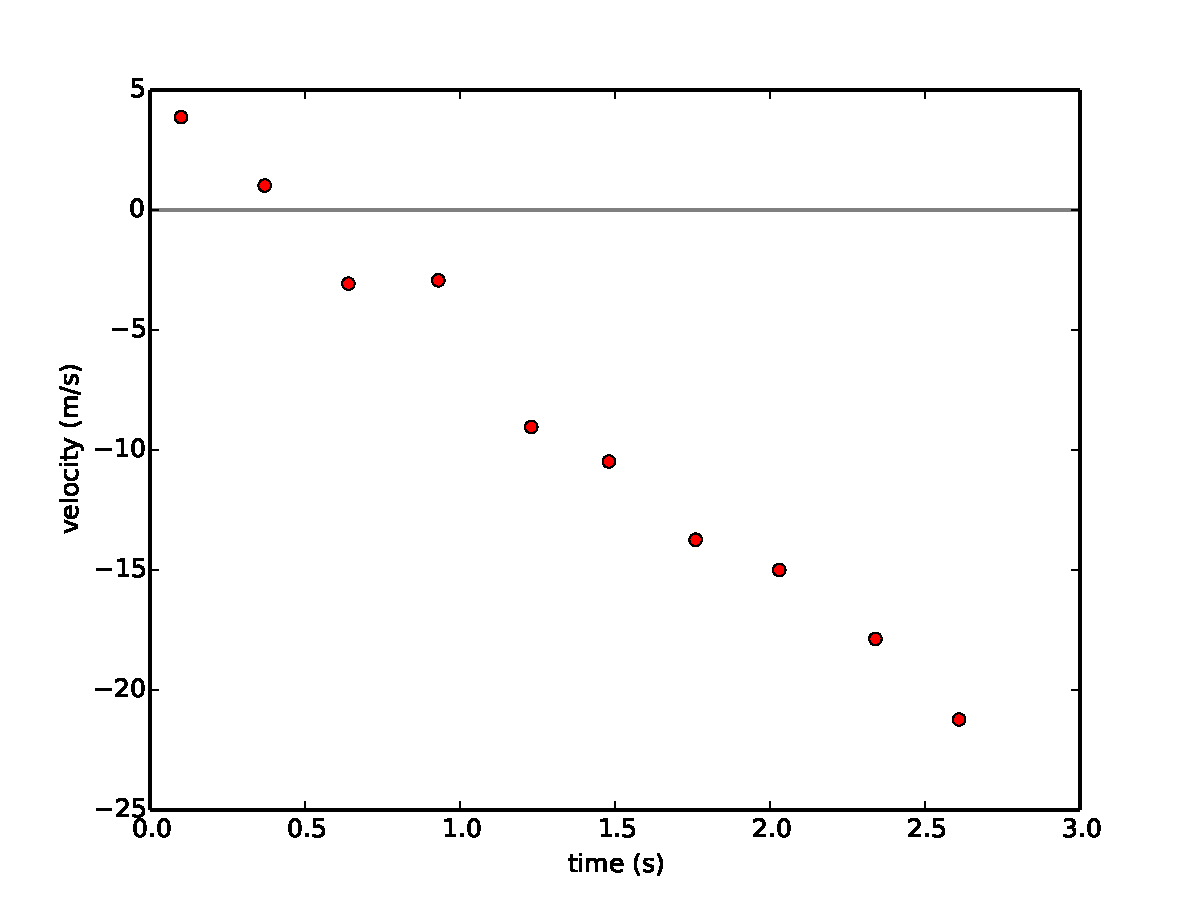
\includegraphics{VelocityVsTimePlot.pdf}}
\caption{Velocity \emph{vs} time for falling mass.}\label{chap7/chap7_funcs:fig-fallingmassdataplot}\end{figure}

While this can give a reasonable estimate of the best fit to the data, the procedure is rather \emph{ad hoc}.  We would prefer to have a more well-defined analytical method for determining what constitutes a ``best fit''.  One way to do that is to consider the sum
\phantomsection\label{chap7/chap7_funcs:equation-eq:lsqrsum}\begin{gather}
\begin{split}S = \sum_{i}^{n} [y_{i} - f(x_{i}; a, b, c, ...)]^2 \;,\end{split}\label{chap7/chap7_funcs-eq:lsqrsum}
\end{gather}
where \(y_{i}\) and \(f(x_{i}; a, b, c, ...)\) are the values of the experimental data and the fitting function, respectively, at \(x_{i}\), and \(S\) is the square of their difference summed over all \(n\) data points.  The quantity \(S\) is a sort of global measure of how much the the fit \(f(x_{i}; a, b, c, ...)\) differs from the experimental data \(y_{i}\).

Notice that for a given set of data points \(\{x_i, y_i\}\), \(S\) is a function only of the fitting parameters \(a, b, ...\), that is, \(S=S(a, b, c, ...)\).  One way of defining a \emph{best} fit, then, is to find the values of the fitting parameters \(a, b, ...\) that minimize the \(S\).

In principle, finding the values of the fitting parameters \(a, b, ...\) that minimize the \(S\) is a simple matter.  Just set the partial derivatives of \(S\) with respect to the fitting parameter equal to zero and solve the resulting system of equations:
\phantomsection\label{chap7/chap7_funcs:equation-eq:sysSzero}\begin{gather}
\begin{split}\frac{\partial S}{\partial a} = 0 \;, \quad
\frac{\partial S}{\partial b} = 0 \;, ...\end{split}\label{chap7/chap7_funcs-eq:sysSzero}
\end{gather}
Because there are as many equations as there are fitting paramters, we should be able to solve the system of equations and find the values of the fitting parameters that minimize \(S\).  Solving those systems of equations is straightforward if the fitting function \(f(x; a, b, ...)\) is linear in the fitting parameters.  Some examples of fitting functions linear in the fitting parameters are:
\phantomsection\label{chap7/chap7_funcs:equation-eq:fitfuncs}\begin{gather}
\begin{split}f(x; a, b) &= a + bx \\
f(x; a, b, c) &= a + bx + cx^2 \\
f(x; a, b, c) &= a \sin x + b e^x + c e^{-x^2} \;.\end{split}\label{chap7/chap7_funcs-eq:fitfuncs}
\end{gather}
For fitting functions such as these, taking the partial derivatives with respect to the fitting parameters, as proposed in \eqref{chap7/chap7_funcs-eq:sysSzero}, results in a set of algebraic equations that are linear in the fitting paramters \(a, b, ...\) Because they are linear, these equations can be solved in a straightforward manner.

For cases in which the fitting function is not linear in the fitting parameters, one can generally still find the values of the fitting parameters that minimize \(S\) but finding them requires more work, which goes beyond our immediate interests here.


\subsection{Linear regression}
\label{chap7/chap7_funcs:linear-regression}
We start by considering the simplest case, fitting a straight line to a data set, such as the one shown in Fig. {\hyperref[chap7/chap7_funcs:fig-fallingmassdataplot]{\emph{4.6}}} above.  Here the fitting function is \(f(x) = a + bx\), which is linear in the fitting parameters \(a\) and \(b\).  For a straight line, the sum in \eqref{chap7/chap7_funcs-eq:lsqrsum} becomes
\phantomsection\label{chap7/chap7_funcs:equation-eq:linreg1}\begin{gather}
\begin{split}S(a,b) = \sum_{i} (y_{i} - a - bx_{i})^2 \;.\end{split}\label{chap7/chap7_funcs-eq:linreg1}
\end{gather}
Finding the best fit in this case corresponds to finding the values of the fitting parameters \(a\) and \(b\) for which \(S(a,b)\) is a minimum.  To find the minimum, we set the derivatives of \(S(a,b)\) equal to zero:
\phantomsection\label{chap7/chap7_funcs:equation-eq:linreg2}\begin{gather}
\begin{split}\frac{\partial S}{\partial a} &= \sum_{i}-2(y_{i}-a-bx_{i}) = 2 \left(na + b\sum_{i}x_{i} - \sum_{i}y_{i} \right) = 0 \\
\frac{\partial S}{\partial b} &= \sum_{i}-2(y_{i}-a-bx_{i})\,x_{i} = 2 \left(a\sum_{i}x_{i} + b\sum_{i}x_{i}^2 - \sum_{i}x_{i}y_{i} \right) = 0\end{split}\label{chap7/chap7_funcs-eq:linreg2}
\end{gather}
Dividing both equations by \(2n\) leads to the equations
\phantomsection\label{chap7/chap7_funcs:equation-eq:ablinreg}\begin{gather}
\begin{split}a + b\bar{x} &= \bar{y}\\
a\bar{x} + b\frac{1}{n}\sum_{i}x_{i}^2  &=  \frac{1}{n}\sum_{i}x_{i}y_{i}\end{split}\label{chap7/chap7_funcs-eq:ablinreg}
\end{gather}
where
\phantomsection\label{chap7/chap7_funcs:equation-eq:linreg3}\begin{gather}
\begin{split}\bar{x} &= \frac{1}{n}\sum_{i}x_{i}\\
\bar{y} &= \frac{1}{n}\sum_{i}y_{i}\;.\end{split}\label{chap7/chap7_funcs-eq:linreg3}
\end{gather}
Solving Eq. \eqref{chap7/chap7_funcs-eq:ablinreg} for the fitting parameters gives
\phantomsection\label{chap7/chap7_funcs:equation-eq:b1}\begin{gather}
\begin{split}b &= \frac{\sum_{i}x_{i}y_{i} - n\bar{x}\bar{y}} {\sum_{i}x_{i}^2 - n \bar{x}^2}\\
a &= \bar{y} - b\bar{x} \;.\end{split}\label{chap7/chap7_funcs-eq:b1}
\end{gather}
Noting that \(n\bar{y}=\sum_{i}y\) and \(n\bar{x}=\sum_{i}x\), the results can be written as
\phantomsection\label{chap7/chap7_funcs:equation-eq:b2}\begin{gather}
\begin{split}b &= \frac{\sum_{i}(x_{i}- \bar{x})\,y_{i}} {\sum_{i}(x_{i}- \bar{x})\,x_{i}} \\
a &= \bar{y} - b\bar{x} \;.\end{split}\label{chap7/chap7_funcs-eq:b2}
\end{gather}
While Eqs. \eqref{chap7/chap7_funcs-eq:b1} and \eqref{chap7/chap7_funcs-eq:b2} are equivalent analytically, Eq. \eqref{chap7/chap7_funcs-eq:b2} is preferred for numerical calculations because Eq. \eqref{chap7/chap7_funcs-eq:b2} is less sensitive to roundoff errors.  Here is a Python function implementing this algorithm:

\begin{Verbatim}[commandchars=\\\{\},numbers=left,firstnumber=1,stepnumber=1]
\PYG{k}{def} \PYG{n+nf}{LineFit}\PYG{p}{(}\PYG{n}{x}\PYG{p}{,} \PYG{n}{y}\PYG{p}{)}\PYG{p}{:}
    \PYG{l+s+sd}{\PYGZsq{}\PYGZsq{}\PYGZsq{} Returns slope and y\PYGZhy{}intercept of linear fit to (x,y)}
\PYG{l+s+sd}{    data set\PYGZsq{}\PYGZsq{}\PYGZsq{}}
    \PYG{n}{xavg} \PYG{o}{=} \PYG{n}{x}\PYG{o}{.}\PYG{n}{mean}\PYG{p}{(}\PYG{p}{)}
    \PYG{n}{slope} \PYG{o}{=} \PYG{p}{(}\PYG{n}{y}\PYG{o}{*}\PYG{p}{(}\PYG{n}{x}\PYG{o}{\PYGZhy{}}\PYG{n}{xavg}\PYG{p}{)}\PYG{p}{)}\PYG{o}{.}\PYG{n}{sum}\PYG{p}{(}\PYG{p}{)}\PYG{o}{/}\PYG{p}{(}\PYG{n}{x}\PYG{o}{*}\PYG{p}{(}\PYG{n}{x}\PYG{o}{\PYGZhy{}}\PYG{n}{xavg}\PYG{p}{)}\PYG{p}{)}\PYG{o}{.}\PYG{n}{sum}\PYG{p}{(}\PYG{p}{)}
    \PYG{n}{yint} \PYG{o}{=} \PYG{n}{y}\PYG{o}{.}\PYG{n}{mean}\PYG{p}{(}\PYG{p}{)}\PYG{o}{\PYGZhy{}}\PYG{n}{slope}\PYG{o}{*}\PYG{n}{xavg}
    \PYG{k}{return} \PYG{n}{slope}\PYG{p}{,} \PYG{n}{yint}
\end{Verbatim}

It's hard to imagine a simpler implementation of the linear regression algorithm.

\index{curve fitting!linear!with weighting}

\subsection{Linear regression with weighting: \(\chi^2\)}
\label{chap7/chap7_funcs:index-6}\label{chap7/chap7_funcs:linear-regression-with-weighting}
The linear regression routine of the previous section weights all data points equally.  That is fine if the absolute uncertainty is the same for all data points.  In many cases, however, the uncertainty is different for different points in a data set.  In such cases, we would like to weight the data that has smaller uncertainty more heavily than those data that have greater uncertainty.  For this case, there is a standard method of weighting and fitting data that is known as \(\chi^2\)  (or \emph{chi-squared}) fitting.  In this method we suppose that associated with each \((x_{i},y_{i})\) data point is an uncertainty in the value of \(y_{i}\) of \(\pm\sigma_{i}\).  In this case, the ``best fit'' is defined as the the one with the set of fitting parameters that minimizes the sum
\phantomsection\label{chap7/chap7_funcs:equation-eq:chisq}\begin{gather}
\begin{split}\chi^2 = \sum_{i} \left(\frac{y_{i} - f(x_{i})} {\sigma_{i}}\right)^2 \;.\end{split}\label{chap7/chap7_funcs-eq:chisq}
\end{gather}
Setting the uncertainties \(\sigma_{i}=1\) for all data points yields the same sum \(S\) we introduced in the previous section.  In this case, all data points are weighted equally.  However, if \(\sigma_{i}\) varies from point to point, it is clear that those points with large \(\sigma_{i}\) contribute less to the sum than those with small \(\sigma_{i}\).  Thus, data points with large \(\sigma_{i}\) are weighted less than those with small \(\sigma_{i}\).

To fit data to a straight line, we set \(f(x) = a + bx\) and write
\phantomsection\label{chap7/chap7_funcs:equation-eq:chisqlin}\begin{gather}
\begin{split}\chi^2(a,b) = \sum_{i} \left(\frac{y_{i} - a -bx_{i}} {\sigma_{i}}\right)^2 \;.\end{split}\label{chap7/chap7_funcs-eq:chisqlin}
\end{gather}
Finding the minimum for \(\chi^2(a,b)\) follows the same procedure used for finding the minimum of \(S(a,b)\) in the previous section.  The result is
\phantomsection\label{chap7/chap7_funcs:equation-eq:abwchisq}\begin{gather}
\begin{split}b &= \frac{\sum_{i}(x_{i} - \hat{x})\,y_{i}/\sigma_{i}^2} {\sum_{i}(x_{i} - \hat{x})\,x_{i}/\sigma_{i}^2}\\
a &= \hat{y} - b\hat{x} \;.\end{split}\label{chap7/chap7_funcs-eq:abwchisq}
\end{gather}
where
\phantomsection\label{chap7/chap7_funcs:equation-eq:xychisq}\begin{gather}
\begin{split}\hat{x} &= \frac{\sum_{i}x_{i}/\sigma_{i}^2} {\sum_{i}1/\sigma_{i}^2}\\
\hat{y} &= \frac{\sum_{i}y_{i}/\sigma_{i}^2} {\sum_{i}1/\sigma_{i}^2}\;.\end{split}\label{chap7/chap7_funcs-eq:xychisq}
\end{gather}
For a fit to a straight line, the overall quality of the fit can be measured by the reduced chi-squared parameter
\phantomsection\label{chap7/chap7_funcs:equation-:eq:linreg13}\begin{gather}
\begin{split}\chi_{r}^2 = \frac{\chi^2}{n-2}\end{split}\label{chap7/chap7_funcs-:eq:linreg13}
\end{gather}
where \(\chi^2\) is given by Eq. \eqref{chap7/chap7_funcs-eq:chisq} evaluated at the optimal values of \(a\) and \(b\) given by Eq. \eqref{chap7/chap7_funcs-eq:abwchisq}.  A good fit is characterized by \(\chi_{r}^2 \approx 1\).  This makes sense because if the uncertainties \(\sigma_{i}\) have been properly estimated, then \([y_{i}-f(x_{i})]^2\) should on average be roughly equal to \(\sigma_{i}^2\), so that the sum in Eq. \eqref{chap7/chap7_funcs-eq:chisq} should consist of \(n\) terms approximately equal to 1.  Of course, if there were only 2 terms (\emph{n=2}), then \(\chi^2\) would be zero as the best straight line fit to two points is a perfect fit.  That is essentially why \(\chi_{r}^2\) is normalized using \(n-2\) instead of \(n\).  If \(\chi_{r}^2\) is significantly greater than 1, this indicates a poor fit to the fitting function (or an underestimation of the uncertainties \(\sigma_{i}\)).  If \(\chi_{r}^2\) is significantly less than 1, then it indicates that the uncertainties were probably overestimated (the fit and fitting function may or may not be good).
\begin{figure}[htbp]
\centering
\capstart

\scalebox{0.800000}{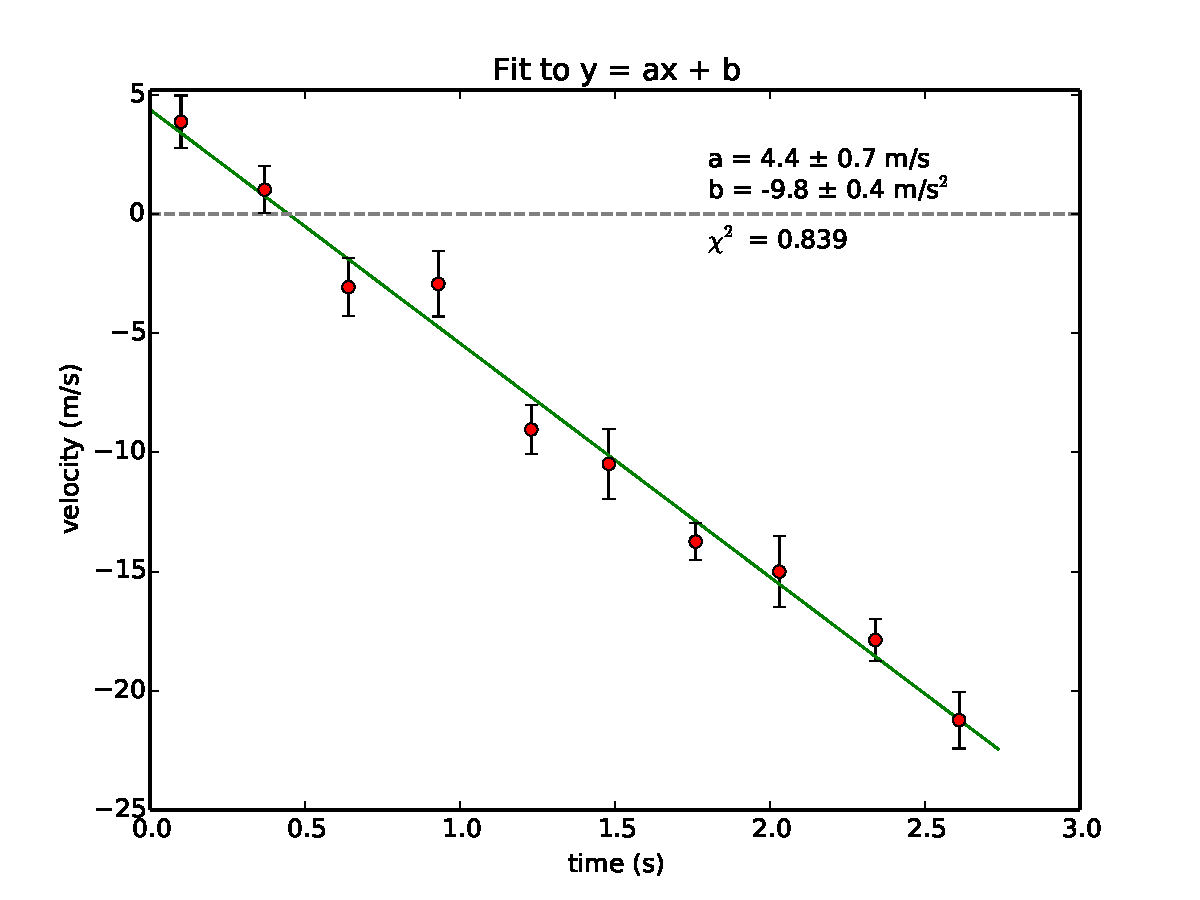
\includegraphics{VelocityVsTimeFit.pdf}}
\caption{Fit using \(\chi^2\) least squares fitting routine with data weighted by error bars.}\label{chap7/chap7_funcs:fig-linregerrbars}\end{figure}

We can also get estimates of the uncertainties in our determination of the fitting parameters \(a\) and \(b\), although deriving the formulas is a bit more involved that we want to get into here.  Therefore, we just give the results:
\phantomsection\label{chap7/chap7_funcs:equation-eq:absigma}\begin{gather}
\begin{split}\sigma_{b}^2 &= \frac{1} {\sum_{i}(x_{i} - \hat{x})\,x_{i}/\sigma_{i}^2}\\
\sigma_{a}^2 &= \sigma_{b}^2 \frac{\sum_{i}x_{i}^2/\sigma_{i}^2} {\sum_{i}1/\sigma_{i}^2}\;.\end{split}\label{chap7/chap7_funcs-eq:absigma}
\end{gather}
The estimates of uncertainties in the fitting parameters depend explicitly on \(\{\sigma_{i}\}\) and will only be meaningful if (\emph{i}) \(\chi_{r}^2 \approx 1\) and (\emph{ii}) the estimates of the uncertainties \(\sigma_{i}\) are accurate.

You can find more information, including a derivation of Eq. \eqref{chap7/chap7_funcs-eq:absigma}, in \emph{Data Reduction and Error Analysis for the Physical Sciences, 3rd ed} by P. R. Bevington \& D. K. Robinson, McGraw-Hill, New York, 2003.

\index{Anonymous functions}\index{Anonymous functions!lambda expressions}\index{lambda expressions}

\section{Anonymous functions (lambda)}
\label{chap7/chap7_funcs:anonymous-functions-lambda}\label{chap7/chap7_funcs:index-7}\label{chap7/chap7_funcs:lambda}
Python provides another way to generate functions called \emph{lambda} expressions.  A lambda expression is a kind of in-line function that can be generated on the fly to accomplish some small task.  You can assign lambda functions a name, but you don't need to; hence, they are often called \emph{anonymous} functions.  A lambda uses the keyword \code{lambda} and has the general form

\begin{Verbatim}[commandchars=\\\{\}]
\PYG{g+go}{lambda arg1, arg2, ... : output}
\end{Verbatim}

The arguments \code{arg1, arg2, ...} are inputs to a lambda, just as for a functions, and the output is an expression using the arguments.

While lambda expressions need not be named, we illustrate their use by comparing a conventional Python function definition to a lambda expression to which we give a name.  First, we define a conventional python function

\begin{Verbatim}[commandchars=\\\{\}]
\PYG{g+gp}{In [1]: }\PYG{k}{def} \PYG{n+nf}{f}\PYG{p}{(}\PYG{n}{a}\PYG{p}{,} \PYG{n}{b}\PYG{p}{)}\PYG{p}{:}
\PYG{g+gp}{   ...:}     \PYG{k}{return} \PYG{l+m+mi}{3}\PYG{o}{*}\PYG{n}{a}\PYG{o}{+}\PYG{n}{b}\PYG{o}{*}\PYG{o}{*}\PYG{l+m+mi}{2}

\PYG{g+gp}{In [2]: }\PYG{n}{f}\PYG{p}{(}\PYG{l+m+mi}{2}\PYG{p}{,}\PYG{l+m+mi}{3}\PYG{p}{)}
\PYG{g+gr}{Out[2]: }\PYG{l+m+mi}{15}
\end{Verbatim}

Next, we define a lambda that does the same thing

\begin{Verbatim}[commandchars=\\\{\}]
\PYG{g+gp}{In [3]: }\PYG{n}{g} \PYG{o}{=} \PYG{k}{lambda} \PYG{n}{a}\PYG{p}{,} \PYG{n}{b} \PYG{p}{:} \PYG{l+m+mi}{3}\PYG{o}{*}\PYG{n}{a}\PYG{o}{+}\PYG{n}{b}\PYG{o}{*}\PYG{o}{*}\PYG{l+m+mi}{2}

\PYG{g+gp}{In [4]: }\PYG{n}{g}\PYG{p}{(}\PYG{l+m+mi}{2}\PYG{p}{,}\PYG{l+m+mi}{3}\PYG{p}{)}
\PYG{g+gr}{Out[4]: }\PYG{l+m+mi}{15}
\end{Verbatim}

The \code{lambda} defined by \code{g} does the same thing as the function \code{f}.  Such \code{lambda} expressions are useful when you need a very short function definition, usually to be used locally only once or a few times.

Sometimes lambda expressions are used in function arguments that call for a function \emph{name}, as opposed to the function itself.  Moreover, in cases where a the function to be integrated is already defined but is a function one independent variable and several parameters, the lambda expression can be a convenient way of fashioning a single variable function.  Don't worry if this doesn't quite make sense to you right now.  You will see examples of lambda expressions used in just this way in the section {\hyperref[chap9/chap9_scipy:numericalintegration]{\emph{Numerical integration}}}.

There are also a number of nifty programming tricks that can be implemented using \code{lambda} expressions, but we will not go into them here.  Look up \code{lambdas} on the web if you are curious about their more exotic uses.
\newpage

\section{Exercises}
\label{chap7/chap7_funcs:exercises}\begin{enumerate}
\item {} 
Write a function that can return each of the first three spherical Bessel functions \(j_n(x)\):
\phantomsection\label{chap7/chap7_funcs:equation-eq:bessel}\begin{gather}
\begin{split}j_0(x) &= \frac{\sin x}{x}\\
j_1(x) &= \frac{\sin x}{x^2} - \frac{\cos x}{x}\\
j_2(x) &= \left(\frac{3}{x^2}-1\right)\frac{\sin x}{x} - \frac{3\cos x}{x^2}\end{split}\label{chap7/chap7_funcs-eq:bessel}
\end{gather}
Your function should take as arguments a NumPy array \(x\) and the order \(n\), and should return an array of the designated order \(n\) spherical Bessel function.  Take care to make sure that your functions behave properly at \(x=0\).

Demonstrate the use of your function by writing a Python routine that plots the three Bessel functions for \(0 \le x \le 20\).  Your plot should look like the one below.  Something to think about: You might note that \(j_1(x)\) can be written in terms of \(j_0(x)\), and that \(j_2(x)\) can be written in terms of \(j_1(x)\) and \(j_0(x)\).  Can you take advantage of this to write a more efficient function for the calculations of \(j_1(x)\) and \(j_2(x)\)?
\begin{figure}[htbp]
\centering

\scalebox{0.800000}{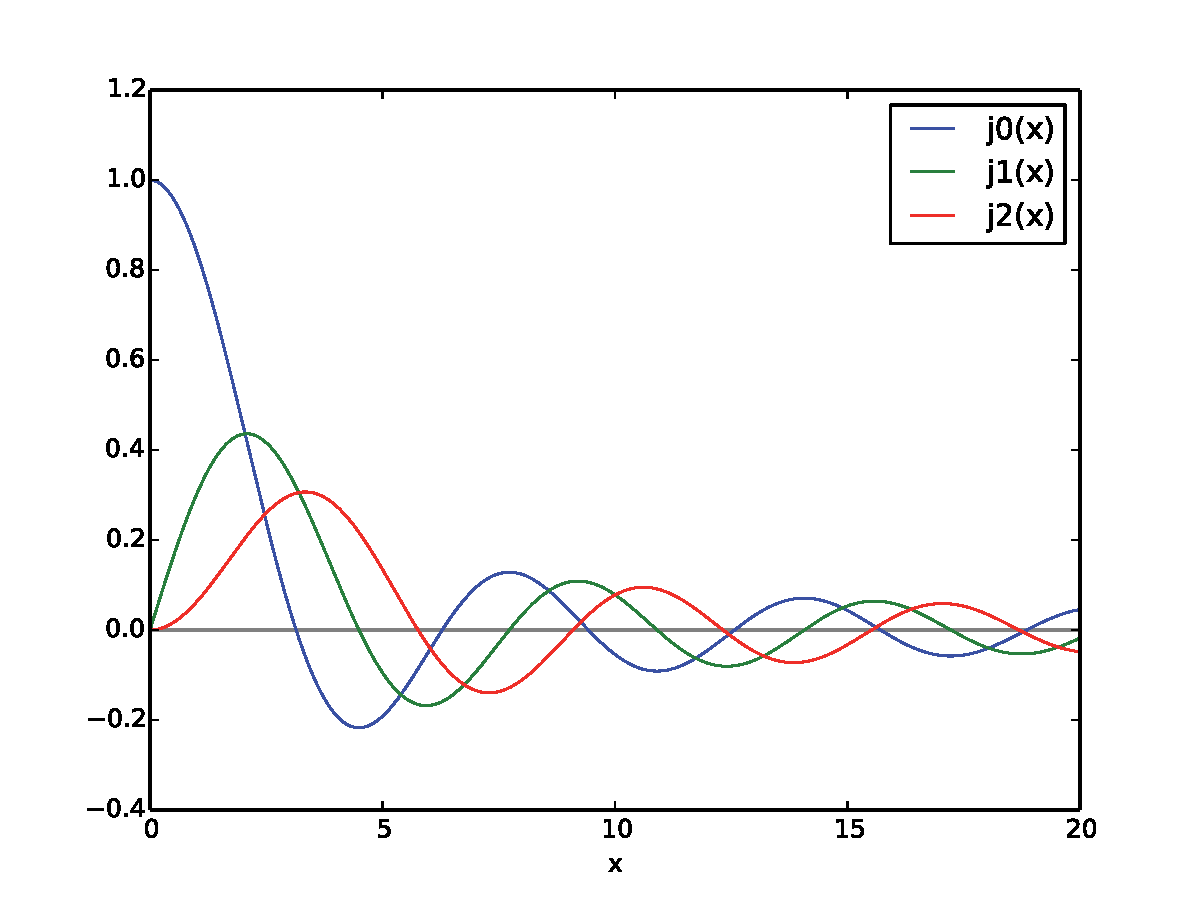
\includegraphics{besselSph.pdf}}
\label{chap7/chap7_funcs:fig-besselsph}\end{figure}

\item {} \begin{enumerate}
\item {} 
Write a function that simulates the rolling of \(n\) dice.  Use the NumPy function \code{random.random\_integers(6)}, which generates a random integer between 1 and 6 with equal probability (like rolling fair dice).  The input of your function should be the number of dice thrown each roll and the output should be the sum of the \(n\) dice.

\item {} 
``Roll'' 2 dice 10,000 times keeping track of all the sums of each set of rolls in a list.  Then use your program to generate a histogram  summarizing the rolls of two dice 10,000 times.  The result should look like the histogram plotted below.  Use the MatPlotLib function \code{hist} (see \href{http://matplotlib.org/api/pyplot\_summary.html}{http://matplotlib.org/api/pyplot\_summary.html}) and set the number of bins in the histogram equal to the number of different possible outcomes of a roll of your dice.  For example, the sum of two dice can be anything between 2 and 12, which corresponds to 11 possible outcomes.  You should get a histogram that looks like the one below.

\item {} 
``Repeat part (b) using 3 dice and plot the resulting histogram.

\end{enumerate}
\begin{figure}[htbp]
\centering

\scalebox{0.800000}{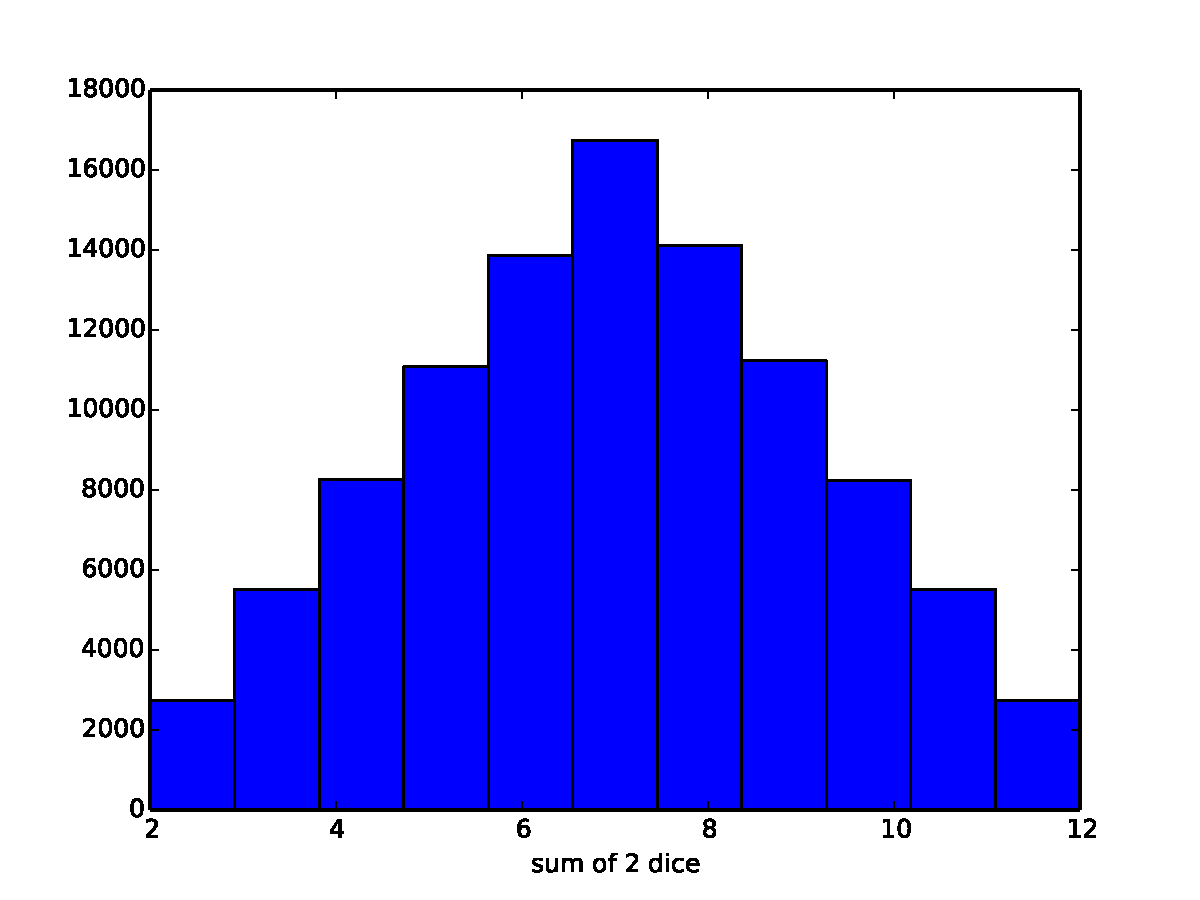
\includegraphics{diceRoll2.pdf}}
\label{chap7/chap7_funcs:fig-dicerolln}\end{figure}

\item {} 
Write a function to draw a circular smiley face with eyes, a nose, and a mouth.  One argument should set the overall size of the face (the circle radius).  Optional arguments should allow the user to specify the \((x,y)\) position of the face, whether the face is smiling or frowning, and the color of the lines.  The default should be a smiling blue face centered at \((0,0)\).  Once you write your function, write a program that calls it several times to produce a plot like the one below (creative improvisation is encouraged!).  In producing your plot, you may find the call \code{plt.axes().set\_aspect(1)} useful so that circles appear as circles and not ovals.  You should only use MatPlotLib functions introduced in this text.  To create a circle you can create an array of angles that goes from 0 to \(2\pi\) and then produce the \(x\) and \(y\) arrays for your circle by taking the cosine and sine, respectively, of the array.  Hint: You can use the same \((x,y)\) arrays to make the smile and frown as you used to make the circle by plotting appropriate slices of those arrays.  You do not need to create new arrays.
\begin{figure}[htbp]
\centering

\scalebox{0.800000}{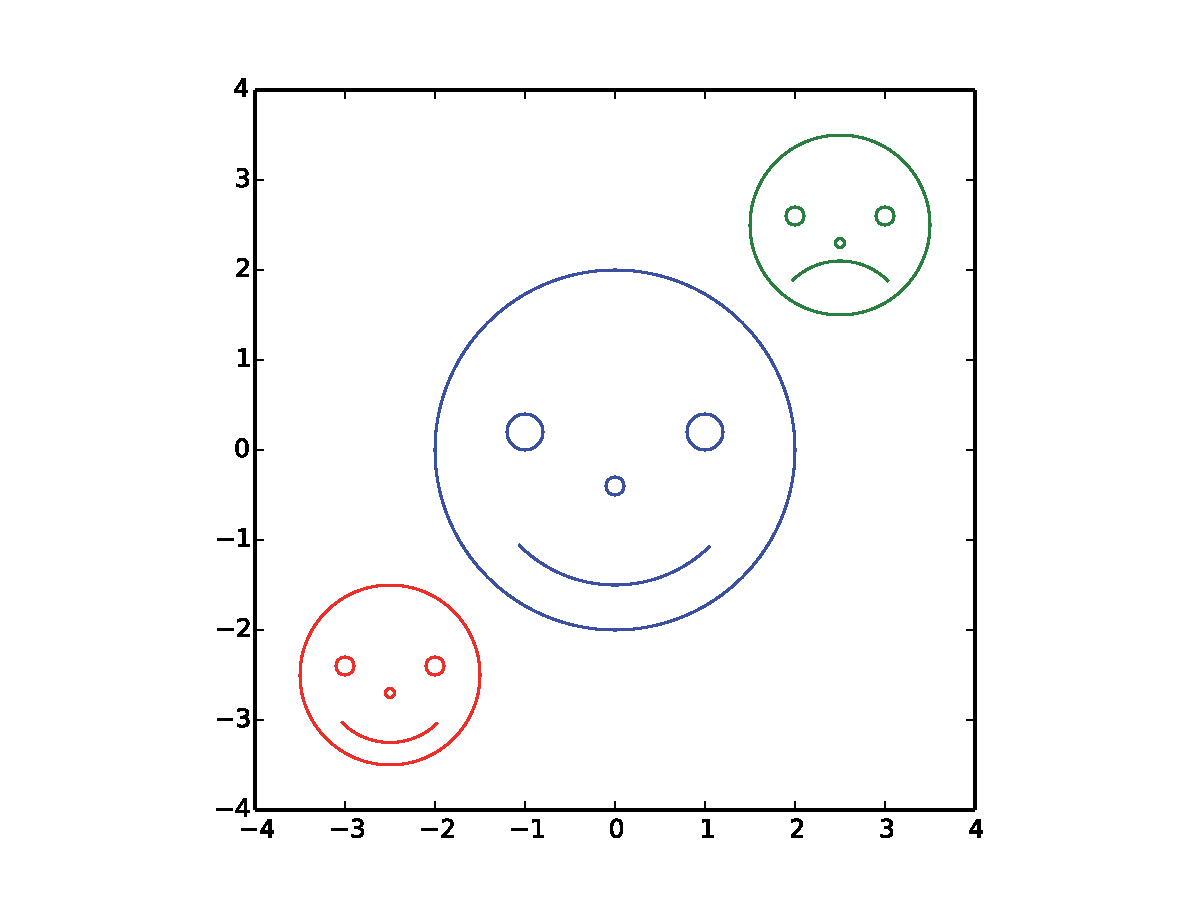
\includegraphics{smiley.pdf}}
\label{chap7/chap7_funcs:fig-faces}\end{figure}

\item {} 
In the section {\hyperref[chap7/chap7_funcs:linfitfunc]{\emph{Example: linear least squares fitting}}}, we showed that the best fit of a line \(y = a + bx\) to a set of data \(\{(x_i,y_i)\}\) is obtained for the values of \(a\) and \(b\) given by Eq. \eqref{chap7/chap7_funcs-eq:b2}.  Those formulas were obtained by finding the values of \(a\) and \(b\) that minimized the sum in Eq. \eqref{chap7/chap7_funcs-eq:linreg1}. This approach and these formulas are valid when the uncertainties in the data are the same for all data points.  The Python function \code{LineFit(x, y)} in the section {\hyperref[chap7/chap7_funcs:linfitfunc]{\emph{Example: linear least squares fitting}}} implements Eq. \eqref{chap7/chap7_funcs-eq:b2}.
\begin{enumerate}
\item {} 
Write a new fitting function \code{LineFitWt(x, y)} that implements the formulas given in Eq. \eqref{chap7/chap7_funcs-eq:xychisq} that minimize the \(\chi^2\) function give by Eq. \eqref{chap7/chap7_funcs-eq:chisqlin}.  This more general approach is valid when the individual data points have different weightings \emph{or} when they all have the same weighting.  You should also write a function to calculate the reduced chi-squared \(\chi_r^2\) defined by Eq. \eqref{chap7/chap7_funcs-eq:chisqlin}.

\item {} 
Write a Python program that reads in the data below, plots it, and fits it using the two fitting functions  \code{LineFit(x, y)} and \code{LineFitWt(x, y)}.  Your program should plot the data with error bars and with \emph{both} fits with and without weighting, that is from \code{LineFit(x, y)} and \code{LineFitWt(x, y, dy)}.  It should also report the results for both fits on the plot, similar to the output of the supplied program above, as well as the values of \(\chi_r^2\), the reduce chi-squared value, for both fits.  Explain why weighting the data gives a steeper or less steep slope than the fit without weighting.

\begin{Verbatim}[commandchars=\\\{\},numbers=left,firstnumber=1,stepnumber=1]
Velocity vs time data
for a falling mass
time (s)   velocity (m/s)   uncertainty (m/s)
  2.23          139               16
  4.78          123               16
  7.21          115                4
  9.37           96                9
 11.64           62               17
 14.23           54               17
 16.55           10               12
 18.70           \PYGZhy{}3               15
 21.05          \PYGZhy{}13               18
 23.21          \PYGZhy{}55               10
\end{Verbatim}

\end{enumerate}

\item {} 
Modify the function \code{LineFitWt(x, y)} you wrote in Exercise 4 above so that in addition to returning the fitting parameters \(a\) and \(b\), it also returns the uncertainties in the fitting parameters \(\sigma_a\) and \(\sigma_b\) using the formulas given by Eq. \eqref{chap7/chap7_funcs-eq:absigma}.  Use your new fitting function to find the uncertainties in the fitted slope and \(y\)-intercept for the data provided with Exercise 4.

\end{enumerate}

\index{curve fitting}

\chapter{Curve Fitting}
\label{chap8/chap8_fitting:index-0}\label{chap8/chap8_fitting::doc}\label{chap8/chap8_fitting:curve-fitting}\label{chap8/chap8_fitting:chap8}
One of the most important tasks in any experimental science is modeling data and determining how well some theoretical function describes experimental data.  In the last chapter, we illustrated how this can be done when the theoretical function is a simple straight line in the context of learning about Python functions and methods.  Here we show how this can be done for a arbitrary fitting functions, including linear, exponential, power law, and other nonlinear fitting functions.


\section{Using linear regression for fitting non-linear functions}
\label{chap8/chap8_fitting:using-linear-regression-for-fitting-non-linear-functions}
We can use our results for linear regression with \(\chi^2\) weighting that we developed in Chapter 7 to fit functions that are nonlinear in the fitting parameters, \emph{provided} we can transform the fitting function into one that is linear in the fitting parameters and in the independent variable (\(x\)).

\index{curve fitting!linear!exponential function}

\subsection{Linear regression for fitting an exponential function}
\label{chap8/chap8_fitting:linear-regression-for-fitting-an-exponential-function}\label{chap8/chap8_fitting:index-1}
To illustrate this approach, let's consider some experimental data taken from a radioactive source that was emitting beta particles (electrons).  We notice that the number of electrons emitted per unit time is decreasing with time.  Theory suggests that the number of electrons \(N\) emitted per unit time should decay exponentially according to the equation
\phantomsection\label{chap8/chap8_fitting:equation-eq:decay}\begin{gather}
\begin{split}N(t) = N_0 e^{-t/\tau} \;.\end{split}\label{chap8/chap8_fitting-eq:decay}
\end{gather}
This equation is nonlinear in \(t\) and in the fitting parameter \(\tau\) and thus cannot be fit using the method of the previous chapter.  Fortunately, this is a special case for which the fitting function can be transformed into a linear form.  Doing so will allow us to use the fitting routine we developed for fitting linear functions.

We begin our analysis by transforming our fitting function to a linear form.  To this end we take the logarithm of Eq. \eqref{chap8/chap8_fitting-eq:decay}:
\begin{gather}
\begin{split}\ln N = \ln N_{0} -\frac{t}{\tau} \;.\end{split}\notag
\end{gather}
With this tranformation our fitting function is linear in the independent variable \(t\).  To make our method work, however, our fitting function must be linear in the \emph{fitting parameters}, and our transformed function is still nonlinear in the fitting parameters \(\tau\) and \(N_0\).  Therefore, we define new fitting parameters as follows
\phantomsection\label{chap8/chap8_fitting:equation-eq:eq15}\begin{gather}
\begin{split}a &= \ln N_{0}\\
b &= -1/\tau\end{split}\label{chap8/chap8_fitting-eq:eq15}
\end{gather}
Now if we define a new dependent variable \(y = \ln N\), then our fitting function takes the form of a fitting function that is linear in the fitting parameters \(a\) and \(b\)
\begin{gather}
\begin{split}y = a + bx\end{split}\notag
\end{gather}
where the independent variable is \(x=t\) and the dependent variable is \(y=\ln N\).

We are almost ready to fit our transformed fitting function, with transformed fitting parameters \(a\) and \(b\), to our transformed independent and dependent data, \(x\) and \(y\).  The last thing we have to do is to transform the estimates of the uncertainties \(\delta N\) in \(N\) to the uncertainties \(\delta y\) in \(y\) \((= \ln N)\).  So how much does a given uncertainty in \(N\) translate into an uncertainty in \(y\)?  In most cases, the uncertainty in \(y\) is much smaller than \(y\), \emph{i.e.} \(\delta y \ll y\); similarly \(\delta N \ll N\).  In this limit we can use differentials to figure out the relationship between these uncertainties.  Here is how it works for this example:
\phantomsection\label{chap8/chap8_fitting:equation-eq:sigmaLnN}\begin{gather}
\begin{split}y &= \ln N\\
\delta y &= \left|\frac{\partial y}{\partial N}\right|\delta N\\
\delta y &= \frac{\delta N} {N} \;.\end{split}\label{chap8/chap8_fitting-eq:sigmaLnN}
\end{gather}
Equation \eqref{chap8/chap8_fitting-eq:sigmaLnN} tells us how a small change \(\delta N\) in \(N\) produces a small change \(\delta y\) in \(y\).  Here we identify the differentials \(dy\) and \(dN\) with the uncertainties \(\delta y\) and \(\delta N\).  Therefore, an uncertainty of \(\delta N\) in \(N\) corresponds, or translates, to an uncertainty \(\delta y\) in \(y\).

Let's summarize what we have done so far.  We started with the some data points \(\{t_i,N_i\}\) and some addition data \(\{\delta N_i\}\) where each datum \(\delta N_i\) corresponds to the uncertainty in the experimentally measured \(N_i\).  We wish to fit these data to the fitting function
\begin{gather}
\begin{split}N(t) = N_0 e^{-t/\tau} \;.\end{split}\notag
\end{gather}
We then take the natural logarithm of both sides and obtain the linear equation
\phantomsection\label{chap8/chap8_fitting:equation-eq:TransformedSemilog}\begin{gather}
\begin{split}\ln N &= \ln N_{0} -\frac{t}{\tau} \\
y &= a + bx\end{split}\label{chap8/chap8_fitting-eq:TransformedSemilog}
\end{gather}
with the obvious correspondences
\phantomsection\label{chap8/chap8_fitting:equation-eq:eqlist}\begin{gather}
\begin{split}x &= t\\
y &= \ln N\\
a &= \ln N_{0}\\
b &= -1/\tau\end{split}\label{chap8/chap8_fitting-eq:eqlist}
\end{gather}
Now we can use the linear regression routine with \(\chi^2\) weighting that we developed in the previous section to fit  \eqref{chap8/chap8_fitting-eq:TransformedSemilog} to the transformed data \(x_i (= t_i)\) and  \(y_i (= \ln N_i)\).  The inputs are the tranformed data \({x_i}, {y_i}, {\delta y_i}\).  The outputs are the fitting parameters \(a\) and \(b\), as well as the estimates of their uncertainties \(\delta a\) and \(\delta b\) along with the value of \(\chi^2\).  You can obtain the values of the original fitting parameters \(N_0\) and \(\tau\) by taking the differentials of the last two equations in Eq. \eqref{chap8/chap8_fitting-eq:eqlist}:
\phantomsection\label{chap8/chap8_fitting:equation-eq:paramunc}\begin{gather}
\begin{split}\delta a &= \left|\frac{\partial a}{\partial N_0}\right|\delta N_0
          = \frac{\delta N_{0}}{N_{0}}\\
\delta b &= \left|\frac{\partial b}{\partial \tau}\right|\delta \tau
          = \frac{\delta \tau}{\tau^2}\end{split}\label{chap8/chap8_fitting-eq:paramunc}
\end{gather}
The Python routine below shows how to implement all of this for a set of experimental data that is read in from a data file.

Figure {\hyperref[chap8/chap8_fitting:fig-betadecay]{\emph{8.1}}} shows the output of the fit to simulated beta decay data obtained using the program below.  Note that the error bars are large when the number of counts \(N\) are small.  This is consistent with what is known as \emph{shot noise} (noise that arises from counting discrete events), which obeys \emph{Poisson} statistics.  You will study sources of noise, including shot noise, later in your lab courses.  The program also prints out the fitting parameters of the transformed data as well as the fitting parameters for the exponential fitting function.
\begin{figure}[htbp]
\centering
\capstart

\scalebox{0.800000}{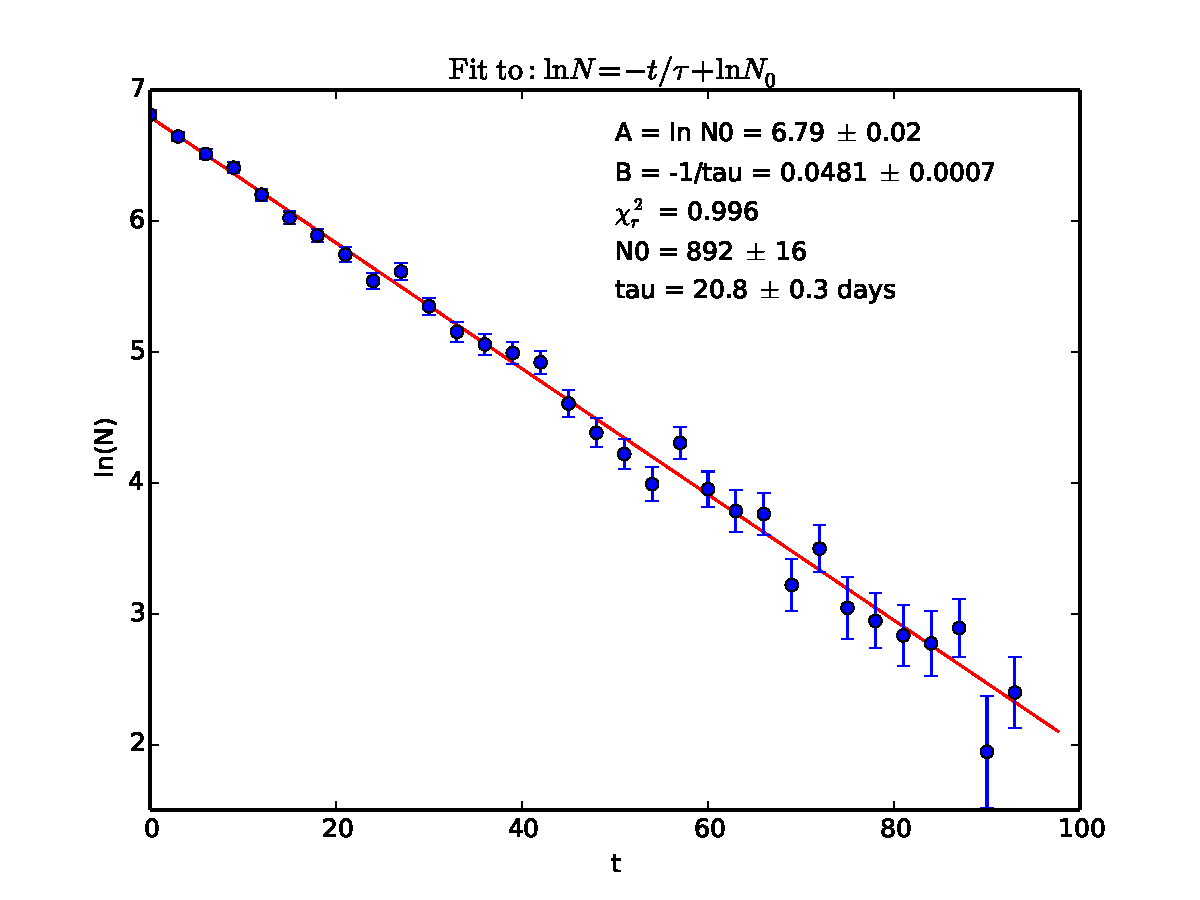
\includegraphics{betaDecay.pdf}}
\caption{Semi-log plot of beta decay measurements from Phosphorus-32.}\label{chap8/chap8_fitting:fig-betadecay}\end{figure}

\begin{Verbatim}[commandchars=\\\{\}]
\PYG{k+kn}{import} \PYG{n+nn}{numpy} \PYG{k+kn}{as} \PYG{n+nn}{np}
\PYG{k+kn}{import} \PYG{n+nn}{matplotlib.pyplot} \PYG{k+kn}{as} \PYG{n+nn}{plt}

\PYG{k}{def} \PYG{n+nf}{LineFitWt}\PYG{p}{(}\PYG{n}{x}\PYG{p}{,} \PYG{n}{y}\PYG{p}{,} \PYG{n}{sig}\PYG{p}{)}\PYG{p}{:}
    \PYG{l+s+sd}{\PYGZdq{}\PYGZdq{}\PYGZdq{}}
\PYG{l+s+sd}{    Fit to straight line.}
\PYG{l+s+sd}{    Inputs: x and y arrays and uncertainty array (unc) for y data.}
\PYG{l+s+sd}{    Ouputs: slope and y\PYGZhy{}intercept of best fit to data.}
\PYG{l+s+sd}{    \PYGZdq{}\PYGZdq{}\PYGZdq{}}
    \PYG{n}{sig2} \PYG{o}{=} \PYG{n}{sig}\PYG{o}{*}\PYG{o}{*}\PYG{l+m+mi}{2}
    \PYG{n}{norm} \PYG{o}{=} \PYG{p}{(}\PYG{l+m+mf}{1.}\PYG{o}{/}\PYG{n}{sig2}\PYG{p}{)}\PYG{o}{.}\PYG{n}{sum}\PYG{p}{(}\PYG{p}{)}
    \PYG{n}{xhat} \PYG{o}{=} \PYG{p}{(}\PYG{n}{x}\PYG{o}{/}\PYG{n}{sig2}\PYG{p}{)}\PYG{o}{.}\PYG{n}{sum}\PYG{p}{(}\PYG{p}{)} \PYG{o}{/} \PYG{n}{norm}
    \PYG{n}{yhat} \PYG{o}{=} \PYG{p}{(}\PYG{n}{y}\PYG{o}{/}\PYG{n}{sig2}\PYG{p}{)}\PYG{o}{.}\PYG{n}{sum}\PYG{p}{(}\PYG{p}{)} \PYG{o}{/} \PYG{n}{norm}
    \PYG{n}{slope} \PYG{o}{=} \PYG{p}{(}\PYG{p}{(}\PYG{n}{x}\PYG{o}{\PYGZhy{}}\PYG{n}{xhat}\PYG{p}{)}\PYG{o}{*}\PYG{n}{y}\PYG{o}{/}\PYG{n}{sig2}\PYG{p}{)}\PYG{o}{.}\PYG{n}{sum}\PYG{p}{(}\PYG{p}{)}\PYG{o}{/}\PYG{p}{(}\PYG{p}{(}\PYG{n}{x}\PYG{o}{\PYGZhy{}}\PYG{n}{xhat}\PYG{p}{)}\PYG{o}{*}\PYG{n}{x}\PYG{o}{/}\PYG{n}{sig2}\PYG{p}{)}\PYG{o}{.}\PYG{n}{sum}\PYG{p}{(}\PYG{p}{)}
    \PYG{n}{yint} \PYG{o}{=} \PYG{n}{yhat} \PYG{o}{\PYGZhy{}} \PYG{n}{slope}\PYG{o}{*}\PYG{n}{xhat}
    \PYG{n}{sig2\PYGZus{}slope} \PYG{o}{=} \PYG{l+m+mf}{1.}\PYG{o}{/}\PYG{p}{(}\PYG{p}{(}\PYG{n}{x}\PYG{o}{\PYGZhy{}}\PYG{n}{xhat}\PYG{p}{)}\PYG{o}{*}\PYG{n}{x}\PYG{o}{/}\PYG{n}{sig2}\PYG{p}{)}\PYG{o}{.}\PYG{n}{sum}\PYG{p}{(}\PYG{p}{)}
    \PYG{n}{sig2\PYGZus{}yint} \PYG{o}{=} \PYG{n}{sig2\PYGZus{}slope} \PYG{o}{*} \PYG{p}{(}\PYG{n}{x}\PYG{o}{*}\PYG{n}{x}\PYG{o}{/}\PYG{n}{sig2}\PYG{p}{)}\PYG{o}{.}\PYG{n}{sum}\PYG{p}{(}\PYG{p}{)} \PYG{o}{/} \PYG{n}{norm}
    \PYG{k}{return} \PYG{n}{slope}\PYG{p}{,} \PYG{n}{yint}\PYG{p}{,} \PYG{n}{np}\PYG{o}{.}\PYG{n}{sqrt}\PYG{p}{(}\PYG{n}{sig2\PYGZus{}slope}\PYG{p}{)}\PYG{p}{,} \PYG{n}{np}\PYG{o}{.}\PYG{n}{sqrt}\PYG{p}{(}\PYG{n}{sig2\PYGZus{}yint}\PYG{p}{)}

\PYG{k}{def} \PYG{n+nf}{redchisq}\PYG{p}{(}\PYG{n}{x}\PYG{p}{,} \PYG{n}{y}\PYG{p}{,} \PYG{n}{dy}\PYG{p}{,} \PYG{n}{slope}\PYG{p}{,} \PYG{n}{yint}\PYG{p}{)}\PYG{p}{:}
    \PYG{n}{chisq} \PYG{o}{=} \PYG{p}{(}\PYG{p}{(}\PYG{p}{(}\PYG{n}{y}\PYG{o}{\PYGZhy{}}\PYG{n}{yint}\PYG{o}{\PYGZhy{}}\PYG{n}{slope}\PYG{o}{*}\PYG{n}{x}\PYG{p}{)}\PYG{o}{/}\PYG{n}{dy}\PYG{p}{)}\PYG{o}{*}\PYG{o}{*}\PYG{l+m+mi}{2}\PYG{p}{)}\PYG{o}{.}\PYG{n}{sum}\PYG{p}{(}\PYG{p}{)}
    \PYG{k}{return} \PYG{n}{chisq}\PYG{o}{/}\PYG{n+nb}{float}\PYG{p}{(}\PYG{n}{x}\PYG{o}{.}\PYG{n}{size}\PYG{o}{\PYGZhy{}}\PYG{l+m+mi}{2}\PYG{p}{)}

\PYG{c}{\PYGZsh{} Read data from data file}
\PYG{n}{t}\PYG{p}{,} \PYG{n}{N}\PYG{p}{,} \PYG{n}{dN} \PYG{o}{=} \PYG{n}{np}\PYG{o}{.}\PYG{n}{loadtxt}\PYG{p}{(}\PYG{l+s}{\PYGZdq{}}\PYG{l+s}{betaDecay.txt}\PYG{l+s}{\PYGZdq{}}\PYG{p}{,} \PYG{n}{skiprows}\PYG{o}{=}\PYG{l+m+mi}{2}\PYG{p}{,} \PYG{n}{unpack}\PYG{o}{=}\PYG{n+nb+bp}{True}\PYG{p}{)}

\PYG{c}{\PYGZsh{}\PYGZsh{}\PYGZsh{}\PYGZsh{}\PYGZsh{}\PYGZsh{}\PYGZsh{}\PYGZsh{}\PYGZsh{}\PYGZsh{} Code to tranform \PYGZam{} fit data starts here \PYGZsh{}\PYGZsh{}\PYGZsh{}\PYGZsh{}\PYGZsh{}\PYGZsh{}\PYGZsh{}\PYGZsh{}\PYGZsh{}\PYGZsh{}}

\PYG{c}{\PYGZsh{} Transform data and parameters to linear form: Y = A + B*X}
\PYG{n}{X} \PYG{o}{=} \PYG{n}{t}         \PYG{c}{\PYGZsh{} transform t data for fitting (trivial)}
\PYG{n}{Y} \PYG{o}{=} \PYG{n}{np}\PYG{o}{.}\PYG{n}{log}\PYG{p}{(}\PYG{n}{N}\PYG{p}{)} \PYG{c}{\PYGZsh{} transform N data for fitting}
\PYG{n}{dY} \PYG{o}{=} \PYG{n}{dN}\PYG{o}{/}\PYG{n}{N}     \PYG{c}{\PYGZsh{} transform uncertainties for fitting}

\PYG{c}{\PYGZsh{} Fit transformed data X, Y, dY to obtain fitting parameters A \PYGZam{} B}
\PYG{c}{\PYGZsh{} Also returns uncertainties in A and B}
\PYG{n}{B}\PYG{p}{,} \PYG{n}{A}\PYG{p}{,} \PYG{n}{dB}\PYG{p}{,} \PYG{n}{dA} \PYG{o}{=} \PYG{n}{LineFitWt}\PYG{p}{(}\PYG{n}{X}\PYG{p}{,} \PYG{n}{Y}\PYG{p}{,} \PYG{n}{dY}\PYG{p}{)}
\PYG{c}{\PYGZsh{} Return reduced chi\PYGZhy{}squared}
\PYG{n}{redchisqr} \PYG{o}{=} \PYG{n}{redchisq}\PYG{p}{(}\PYG{n}{X}\PYG{p}{,} \PYG{n}{Y}\PYG{p}{,} \PYG{n}{dY}\PYG{p}{,} \PYG{n}{B}\PYG{p}{,} \PYG{n}{A}\PYG{p}{)}

\PYG{c}{\PYGZsh{} Determine fitting parameters for original exponential function}
\PYG{c}{\PYGZsh{} N = N0 exp(\PYGZhy{}t/tau) ...}
\PYG{n}{N0} \PYG{o}{=} \PYG{n}{np}\PYG{o}{.}\PYG{n}{exp}\PYG{p}{(}\PYG{n}{A}\PYG{p}{)}
\PYG{n}{tau} \PYG{o}{=} \PYG{o}{\PYGZhy{}}\PYG{l+m+mf}{1.0}\PYG{o}{/}\PYG{n}{B}
\PYG{c}{\PYGZsh{} ... and their uncertainties}
\PYG{n}{dN0} \PYG{o}{=} \PYG{n}{N0} \PYG{o}{*} \PYG{n}{dA}
\PYG{n}{dtau} \PYG{o}{=} \PYG{n}{tau}\PYG{o}{*}\PYG{o}{*}\PYG{l+m+mi}{2} \PYG{o}{*} \PYG{n}{dB}

\PYG{c}{\PYGZsh{}\PYGZsh{}\PYGZsh{}\PYGZsh{}\PYGZsh{}\PYGZsh{}\PYGZsh{} Code to plot transformed data and fit starts here \PYGZsh{}\PYGZsh{}\PYGZsh{}\PYGZsh{}\PYGZsh{}\PYGZsh{}\PYGZsh{}}

\PYG{c}{\PYGZsh{} Create line corresponding to fit using fitting parameters}
\PYG{c}{\PYGZsh{} Only two points are needed to specify a straight line}
\PYG{n}{Xext} \PYG{o}{=} \PYG{l+m+mf}{0.05}\PYG{o}{*}\PYG{p}{(}\PYG{n}{X}\PYG{o}{.}\PYG{n}{max}\PYG{p}{(}\PYG{p}{)}\PYG{o}{\PYGZhy{}}\PYG{n}{X}\PYG{o}{.}\PYG{n}{min}\PYG{p}{(}\PYG{p}{)}\PYG{p}{)}
\PYG{n}{Xfit} \PYG{o}{=} \PYG{n}{np}\PYG{o}{.}\PYG{n}{array}\PYG{p}{(}\PYG{p}{[}\PYG{n}{X}\PYG{o}{.}\PYG{n}{min}\PYG{p}{(}\PYG{p}{)}\PYG{o}{\PYGZhy{}}\PYG{n}{Xext}\PYG{p}{,} \PYG{n}{X}\PYG{o}{.}\PYG{n}{max}\PYG{p}{(}\PYG{p}{)}\PYG{o}{+}\PYG{n}{Xext}\PYG{p}{]}\PYG{p}{)}
\PYG{n}{Yfit} \PYG{o}{=} \PYG{n}{A} \PYG{o}{+} \PYG{n}{B}\PYG{o}{*}\PYG{n}{Xfit}

\PYG{n}{plt}\PYG{o}{.}\PYG{n}{errorbar}\PYG{p}{(}\PYG{n}{X}\PYG{p}{,} \PYG{n}{Y}\PYG{p}{,} \PYG{n}{dY}\PYG{p}{,} \PYG{n}{fmt}\PYG{o}{=}\PYG{l+s}{\PYGZdq{}}\PYG{l+s}{bo}\PYG{l+s}{\PYGZdq{}}\PYG{p}{)}
\PYG{n}{plt}\PYG{o}{.}\PYG{n}{plot}\PYG{p}{(}\PYG{n}{Xfit}\PYG{p}{,} \PYG{n}{Yfit}\PYG{p}{,} \PYG{l+s}{\PYGZdq{}}\PYG{l+s}{r\PYGZhy{}}\PYG{l+s}{\PYGZdq{}}\PYG{p}{,} \PYG{n}{zorder}\PYG{o}{=}\PYG{o}{\PYGZhy{}}\PYG{l+m+mi}{1}\PYG{p}{)}
\PYG{n}{plt}\PYG{o}{.}\PYG{n}{xlim}\PYG{p}{(}\PYG{l+m+mi}{0}\PYG{p}{,} \PYG{l+m+mi}{100}\PYG{p}{)}
\PYG{n}{plt}\PYG{o}{.}\PYG{n}{ylim}\PYG{p}{(}\PYG{l+m+mf}{1.5}\PYG{p}{,} \PYG{l+m+mi}{7}\PYG{p}{)}
\PYG{n}{plt}\PYG{o}{.}\PYG{n}{title}\PYG{p}{(}\PYG{l+s}{\PYGZdq{}}\PYG{l+s}{\PYGZdl{}}\PYG{l+s}{\PYGZbs{}}\PYG{l+s}{mathrm\PYGZob{}Fit}\PYG{l+s+se}{\PYGZbs{}\PYGZbs{}}\PYG{l+s}{ to:\PYGZcb{}}\PYG{l+s+se}{\PYGZbs{}\PYGZbs{}}\PYG{l+s}{ }\PYG{l+s}{\PYGZbs{}}\PYG{l+s}{ln N = \PYGZhy{}t/}\PYG{l+s+se}{\PYGZbs{}\PYGZbs{}}\PYG{l+s}{tau + }\PYG{l+s}{\PYGZbs{}}\PYG{l+s}{ln N\PYGZus{}0\PYGZdl{}}\PYG{l+s}{\PYGZdq{}}\PYG{p}{)}
\PYG{n}{plt}\PYG{o}{.}\PYG{n}{xlabel}\PYG{p}{(}\PYG{l+s}{\PYGZdq{}}\PYG{l+s}{t}\PYG{l+s}{\PYGZdq{}}\PYG{p}{)}
\PYG{n}{plt}\PYG{o}{.}\PYG{n}{ylabel}\PYG{p}{(}\PYG{l+s}{\PYGZdq{}}\PYG{l+s}{ln(N)}\PYG{l+s}{\PYGZdq{}}\PYG{p}{)}

\PYG{n}{plt}\PYG{o}{.}\PYG{n}{text}\PYG{p}{(}\PYG{l+m+mi}{50}\PYG{p}{,} \PYG{l+m+mf}{6.6}\PYG{p}{,} \PYG{l+s}{\PYGZdq{}}\PYG{l+s}{A = ln N0 = \PYGZob{}0:0.2f\PYGZcb{} \PYGZdl{}}\PYG{l+s}{\PYGZbs{}}\PYG{l+s}{pm\PYGZdl{} \PYGZob{}1:0.2f\PYGZcb{}}\PYG{l+s}{\PYGZdq{}}
         \PYG{o}{.}\PYG{n}{format}\PYG{p}{(}\PYG{n}{A}\PYG{p}{,} \PYG{n}{dA}\PYG{p}{)}\PYG{p}{)}
\PYG{n}{plt}\PYG{o}{.}\PYG{n}{text}\PYG{p}{(}\PYG{l+m+mi}{50}\PYG{p}{,} \PYG{l+m+mf}{6.3}\PYG{p}{,} \PYG{l+s}{\PYGZdq{}}\PYG{l+s}{B = \PYGZhy{}1/tau = \PYGZob{}0:0.4f\PYGZcb{} \PYGZdl{}}\PYG{l+s}{\PYGZbs{}}\PYG{l+s}{pm\PYGZdl{} \PYGZob{}1:0.4f\PYGZcb{}}\PYG{l+s}{\PYGZdq{}}
         \PYG{o}{.}\PYG{n}{format}\PYG{p}{(}\PYG{o}{\PYGZhy{}}\PYG{n}{B}\PYG{p}{,} \PYG{n}{dB}\PYG{p}{)}\PYG{p}{)}
\PYG{n}{plt}\PYG{o}{.}\PYG{n}{text}\PYG{p}{(}\PYG{l+m+mi}{50}\PYG{p}{,} \PYG{l+m+mf}{6.0}\PYG{p}{,} \PYG{l+s}{\PYGZdq{}}\PYG{l+s}{\PYGZdl{}}\PYG{l+s}{\PYGZbs{}}\PYG{l+s}{chi\PYGZus{}r\PYGZca{}2\PYGZdl{} = \PYGZob{}0:0.3f\PYGZcb{}}\PYG{l+s}{\PYGZdq{}}
         \PYG{o}{.}\PYG{n}{format}\PYG{p}{(}\PYG{n}{redchisqr}\PYG{p}{)}\PYG{p}{)}

\PYG{n}{plt}\PYG{o}{.}\PYG{n}{text}\PYG{p}{(}\PYG{l+m+mi}{50}\PYG{p}{,} \PYG{l+m+mf}{5.7}\PYG{p}{,} \PYG{l+s}{\PYGZdq{}}\PYG{l+s}{N0 = \PYGZob{}0:0.0f\PYGZcb{} \PYGZdl{}}\PYG{l+s}{\PYGZbs{}}\PYG{l+s}{pm\PYGZdl{} \PYGZob{}1:0.0f\PYGZcb{}}\PYG{l+s}{\PYGZdq{}}
         \PYG{o}{.}\PYG{n}{format}\PYG{p}{(}\PYG{n}{N0}\PYG{p}{,} \PYG{n}{dN0}\PYG{p}{)}\PYG{p}{)}
\PYG{n}{plt}\PYG{o}{.}\PYG{n}{text}\PYG{p}{(}\PYG{l+m+mi}{50}\PYG{p}{,} \PYG{l+m+mf}{5.4}\PYG{p}{,} \PYG{l+s}{\PYGZdq{}}\PYG{l+s}{tau = \PYGZob{}0:0.1f\PYGZcb{} \PYGZdl{}}\PYG{l+s}{\PYGZbs{}}\PYG{l+s}{pm\PYGZdl{} \PYGZob{}1:0.1f\PYGZcb{} days}\PYG{l+s}{\PYGZdq{}}
         \PYG{o}{.}\PYG{n}{format}\PYG{p}{(}\PYG{n}{tau}\PYG{p}{,} \PYG{n}{dtau}\PYG{p}{)}\PYG{p}{)}

\PYG{n}{plt}\PYG{o}{.}\PYG{n}{show}\PYG{p}{(}\PYG{p}{)}
\end{Verbatim}

\index{curve fitting!linear!power law function}
\index{curve fitting!linear!power-law function}

\subsection{Linear regression for fitting a power-law function}
\label{chap8/chap8_fitting:linear-regression-for-fitting-a-power-law-function}\label{chap8/chap8_fitting:index-3}
You can use a similar approach to the one outlined above to fit experimental data to a power law fitting function of the form
\phantomsection\label{chap8/chap8_fitting:equation-eq:pwrlaw}\begin{gather}
\begin{split}P(s) = P_0 s^\alpha \;.\end{split}\label{chap8/chap8_fitting-eq:pwrlaw}
\end{gather}
We follow the same approach we used for the exponential fitting function and first take the logarithm of both sides of \eqref{chap8/chap8_fitting-eq:pwrlaw}
\phantomsection\label{chap8/chap8_fitting:equation-eq:logpwrlaw}\begin{gather}
\begin{split}\ln P = \ln P_0 + \alpha \ln s \;.\end{split}\label{chap8/chap8_fitting-eq:logpwrlaw}
\end{gather}
We recast this in the form of a linear equation \(y = a + bx\) with the following identifications:
\phantomsection\label{chap8/chap8_fitting:equation-eq:eqPwrTrans}\begin{gather}
\begin{split}x &= \ln s\\
y &= \ln P\\
a &= \ln P_{0}\\
b &= \alpha\end{split}\label{chap8/chap8_fitting-eq:eqPwrTrans}
\end{gather}
Following a procedure similar to that used to fit using an exponential fitting function, you can use the tranformations given by \eqref{chap8/chap8_fitting-eq:eqPwrTrans} as the basis for a program to fit a power-law fitting function such as \eqref{chap8/chap8_fitting-eq:logpwrlaw} to experimental data.

\index{curve fitting!nonlinear}

\section{Nonlinear fitting}
\label{chap8/chap8_fitting:index-4}\label{chap8/chap8_fitting:sec-nonlinfit}\label{chap8/chap8_fitting:nonlinear-fitting}
The method introduced in the previous section for fitting nonlinear fitting functions can be used only if the fitting function can be transformed into a fitting function that is linear in the fitting parameters  \(a\), \(b\), \(c\)...  When we have a nonlinear fitting function that cannot be transformed into a linear form, we need another approach.

The problem of finding values of the fitting parameters that minimize \(\chi^2\) is a nonlinear optimization problem to which there is quite generally no analytical solution (in contrast to the linear optimization problem).  We can gain some insight into this nonlinear optimization problem, namely the fitting of a nonlinear fitting function to a data set, by considering a fitting function with only two fitting parameters.  That is, we are trying to fit some data set \(\{x_{i},y_{i}\}\), with uncertainties in \(\{y_{i}\}\) of \(\{\sigma_{i}\}\), to a fitting function is \(f(x;a,b)\) where \(a\) and \(b\) are the two fitting parameters.  To do so, we look for the minimum in
\begin{gather}
\begin{split}\chi^2(a,b) = \sum_{i} \left(\frac{y_{i} - f(x_{i})}{\sigma_{i}}\right)^2 \;.\end{split}\notag
\end{gather}
Note that once the data set, uncertainties, and fitting function are specified,  \(\chi^2(a,b)\) is simply a function of \(a\) and \(b\).  We can picture the function \(\chi^2(a,b)\) as a of landscape with peaks and valleys: as we vary \(a\) and \(b\), \(\chi^2(a,b)\) rises and falls.  The basic idea of all nonlinear fitting routines is to start with some initial guesses for the fitting parameters, here \(a\) and \(b\), and by scanning the \(\chi^2(a,b)\) landscape, find values of \(a\) and \(b\) that minimize \(\chi^2(a,b)\).

There are a number of different methods for trying to find the minimum in \(\chi^2\) for nonlinear fitting problems.  Nevertheless, the method that is most widely used goes by the name of the \emph{Levenberg-Marquardt} method.  Actually the Levenberg-Marquardt method is a combination of two other methods, the \emph{steepest descent} (or gradient) method and \emph{parabolic extrapolation}.  Roughly speaking, when the values of \(a\) and \(b\) are not too near their optimal values, the gradient descent method determines in which direction in \((a,b)\)-space the function \(\chi^2(a,b)\) decreases most quickly---the direction of steepest descent---and then changes \(a\) and \(b\) accordingly to move in that direction.  This method is very efficient unless \(a\) and \(b\) are very near their optimal values.  Near the optimal values of \(a\) and \(b\), parabolic extrapolation is more efficient.  Therefore, as  \(a\) and \(b\) approach their optimal values, the Levenberg-Marquardt method gradually changes to the parabolic extrapolation method, which approximates \(\chi^2(a,b)\) by a Taylor series second order in \(a\) and \(b\) and then computes directly the analytical minimum of the Taylor series approximation of \(\chi^2(a,b)\).  This method is only good if the second order Taylor series provides a good approximation of \(\chi^2(a,b)\).  That is why parabolic extrapolation only works well very near the minimum in \(\chi^2(a,b)\).

Before illustrating the Levenberg-Marquardt method, we make one important cautionary remark: the Levenberg-Marquardt method can fail if the initial guesses of the fitting parameters are too far away from the desired solution.  This problem becomes more serious the greater the number of fitting parameters.  Thus it is important to provide reasonable initial guesses for the fitting parameters.  Usually, this is not a problem, as it is clear from the physical situation of a particular experiment what reasonable values of the fitting parameters are.  But beware!

The \code{scipy.optimize} module provides routines that implement the Levenberg-Marquardt non-linear fitting method.  One is called \code{scipy.optimize.leastsq}.  A somewhat more user-friendly version of the same method is accessed through another routine in the same \code{scipy.optimize} module: it's called \code{scipy.optimize.curve\_fit} and it is the one we demonstrate here.  The function call is

\begin{Verbatim}[commandchars=\\\{\}]
import scipy.optimize
[... insert code here ...]
scipy.optimize.curve\PYGZus{}fit(f, xdata, ydata, p0=None, sigma=None,
                         **kwargs)
\end{Verbatim}

The arguments of \code{curve\_fit} are
\begin{itemize}
\item {} 
\code{f(xdata, a, b, ...)}: is the fitting function where \code{xdata} is the data for the independent variable and \code{a, b, ...} are the fitting parameters, however many there are, listed as separate arguments.  Obviously, \code{f(xdata, a, b, ...)} should return the \(y\) value of the fitting function.

\item {} 
\code{xdata}: is the array containing the \(x\) data.

\item {} 
\code{ydata}: is the array containing the \(y\) data.

\item {} 
\code{p0}: is a tuple containing the initial guesses for the fitting parameters.  The guesses for the fitting parameters are set equal to 1 if they are left unspecified.  It is almost always a good idea to specify the initial guesses for the fitting parameters.

\item {} 
\code{sigma}: is the array containing the uncertainties in the \(y\) data.

\item {} 
\code{**kwargs}: are keyword arguments that can be passed to the fitting routine \code{scipy.optimize.leastsq} that \code{curve\_fit} calls.  These are usually left unspecified.

\end{itemize}

We demonstrate the use of \code{curve\_fit} to fit the data plotted in the figure below:
\begin{figure}[htbp]
\centering

\scalebox{0.800000}{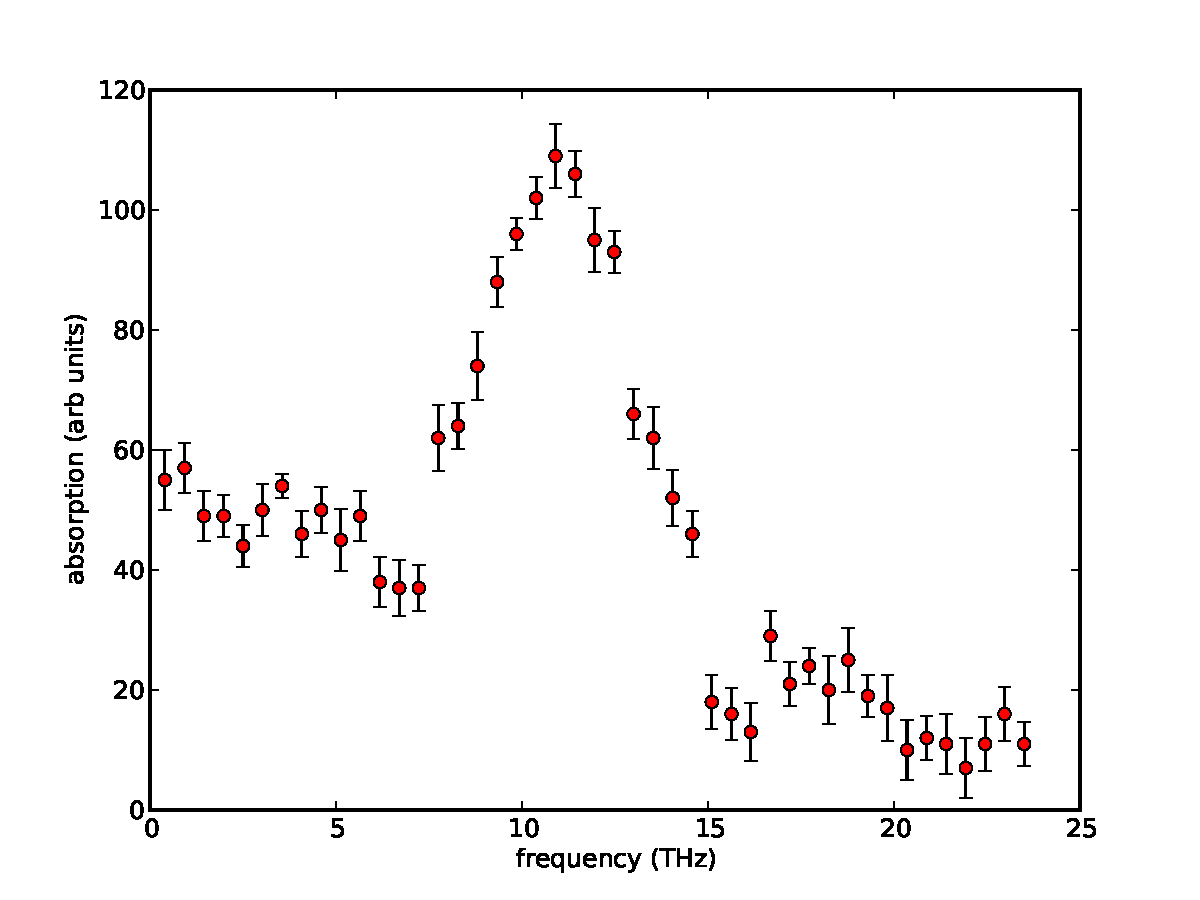
\includegraphics{Spectrum.pdf}}
\label{chap8/chap8_fitting:fig-spectrum}\end{figure}

We model the data with the fitting function that consists of a quadratic polynomial background with a Gaussian peak:
\begin{gather}
\begin{split}A(f) = a + bf + cf^2 + P e^{-\frac{1}{2}[(f-f_p)/f_w]^2} .\end{split}\notag
\end{gather}
Lines 7 and 8 define the fitting functions.  Note that the independent variable \code{f} is the first argument, which is followed by the six fitting parameters \(a\), \(b\), \(c\), \(P\), \(f_p\), and \(f_w\).

To fit the data with \(A(f)\), we need good estimates of the fitting parameters.  Setting \(f=0\), we see that \(a \approx 60\).  An estimate of the slope of the baseline gives \(b \approx -60/20=-3\).  The curvature in the baseline is small so we take \(c \approx 0\).  The amplitude of the peak above the baseline is \(P \approx 110-30=80\).  The peak is centered at \(f_p \approx 11\), while width of peak is about \(f_w \approx 2\).  We use these estimates to set the initial guesses of the fitting parameters in lines 14 and 15 in the code below.

\index{list comprehension}
The function that performs the Levenverg-Marquardt algorithm, \emph{scipy.optimize.curve\_fit}, is called in lines 19-20 with the output set equal to the one and two-dimensional arrays \code{nlfit} and \code{nlpcov}, respectively.  The array \code{nlfit}, which gives the optimal values of the  fitting parameters, is unpacked in line 23.  The square root of the diagonal of the two-dimensional array \code{nlpcov}, which gives the estimates of the uncertainties in the fitting parameters, is unpacked in lines 26-27 using a list comprehension.

The rest of the code plots the data, the fitting function using the optimal values of the fitting parameters found by \code{scipy.optimize.curve\_fit}, and the values of the fitting parameters and their uncertainties.

\begin{Verbatim}[commandchars=\\\{\},numbers=left,firstnumber=1,stepnumber=1]
\PYG{k+kn}{import} \PYG{n+nn}{numpy} \PYG{k+kn}{as} \PYG{n+nn}{np}
\PYG{k+kn}{import} \PYG{n+nn}{matplotlib.pyplot} \PYG{k+kn}{as} \PYG{n+nn}{plt}
\PYG{k+kn}{import} \PYG{n+nn}{matplotlib.gridspec} \PYG{k+kn}{as} \PYG{n+nn}{gridspec}  \PYG{c}{\PYGZsh{} for unequal plot boxes}
\PYG{k+kn}{import} \PYG{n+nn}{scipy.optimize}

\PYG{c}{\PYGZsh{} define fitting function}
\PYG{k}{def} \PYG{n+nf}{GaussPolyBase}\PYG{p}{(}\PYG{n}{f}\PYG{p}{,} \PYG{n}{a}\PYG{p}{,} \PYG{n}{b}\PYG{p}{,} \PYG{n}{c}\PYG{p}{,} \PYG{n}{P}\PYG{p}{,} \PYG{n}{fp}\PYG{p}{,} \PYG{n}{fw}\PYG{p}{)}\PYG{p}{:}
    \PYG{k}{return} \PYG{n}{a} \PYG{o}{+} \PYG{n}{b}\PYG{o}{*}\PYG{n}{f} \PYG{o}{+} \PYG{n}{c}\PYG{o}{*}\PYG{n}{f}\PYG{o}{*}\PYG{n}{f} \PYG{o}{+} \PYG{n}{P}\PYG{o}{*}\PYG{n}{np}\PYG{o}{.}\PYG{n}{exp}\PYG{p}{(}\PYG{o}{\PYGZhy{}}\PYG{l+m+mf}{0.5}\PYG{o}{*}\PYG{p}{(}\PYG{p}{(}\PYG{n}{f}\PYG{o}{\PYGZhy{}}\PYG{n}{fp}\PYG{p}{)}\PYG{o}{/}\PYG{n}{fw}\PYG{p}{)}\PYG{o}{*}\PYG{o}{*}\PYG{l+m+mi}{2}\PYG{p}{)}

\PYG{c}{\PYGZsh{} read in spectrum from data file}
\PYG{c}{\PYGZsh{} f=frequency, s=signal, ds=s uncertainty}
\PYG{n}{f}\PYG{p}{,} \PYG{n}{s}\PYG{p}{,} \PYG{n}{ds} \PYG{o}{=} \PYG{n}{np}\PYG{o}{.}\PYG{n}{loadtxt}\PYG{p}{(}\PYG{l+s}{\PYGZdq{}}\PYG{l+s}{Spectrum.txt}\PYG{l+s}{\PYGZdq{}}\PYG{p}{,} \PYG{n}{skiprows}\PYG{o}{=}\PYG{l+m+mi}{4}\PYG{p}{,} \PYG{n}{unpack}\PYG{o}{=}\PYG{n+nb+bp}{True}\PYG{p}{)}

\PYG{c}{\PYGZsh{} initial guesses for fitting parameters}
\PYG{n}{a0}\PYG{p}{,} \PYG{n}{b0}\PYG{p}{,} \PYG{n}{c0} \PYG{o}{=} \PYG{l+m+mf}{60.}\PYG{p}{,} \PYG{o}{\PYGZhy{}}\PYG{l+m+mf}{3.}\PYG{p}{,} \PYG{l+m+mf}{0.}
\PYG{n}{P0}\PYG{p}{,} \PYG{n}{fp0}\PYG{p}{,} \PYG{n}{fw0} \PYG{o}{=} \PYG{l+m+mf}{80.}\PYG{p}{,} \PYG{l+m+mf}{11.}\PYG{p}{,} \PYG{l+m+mf}{2.}

\PYG{c}{\PYGZsh{} fit data using SciPy\PYGZsq{}s Levenberg\PYGZhy{}Marquart method}
\PYG{n}{nlfit}\PYG{p}{,} \PYG{n}{nlpcov} \PYG{o}{=} \PYG{n}{scipy}\PYG{o}{.}\PYG{n}{optimize}\PYG{o}{.}\PYG{n}{curve\PYGZus{}fit}\PYG{p}{(}\PYG{n}{GaussPolyBase}\PYG{p}{,}
                \PYG{n}{f}\PYG{p}{,} \PYG{n}{s}\PYG{p}{,} \PYG{n}{p0}\PYG{o}{=}\PYG{p}{[}\PYG{n}{a0}\PYG{p}{,} \PYG{n}{b0}\PYG{p}{,} \PYG{n}{c0}\PYG{p}{,} \PYG{n}{P0}\PYG{p}{,} \PYG{n}{fp0}\PYG{p}{,} \PYG{n}{fw0}\PYG{p}{]}\PYG{p}{,} \PYG{n}{sigma}\PYG{o}{=}\PYG{n}{ds}\PYG{p}{)}

\PYG{c}{\PYGZsh{} unpack fitting parameters}
\PYG{n}{a}\PYG{p}{,} \PYG{n}{b}\PYG{p}{,} \PYG{n}{c}\PYG{p}{,} \PYG{n}{P}\PYG{p}{,} \PYG{n}{fp}\PYG{p}{,} \PYG{n}{fw} \PYG{o}{=} \PYG{n}{nlfit}
\PYG{c}{\PYGZsh{} unpack uncertainties in fitting parameters from diagonal}
\PYG{c}{\PYGZsh{} of covariance matrix}
\PYG{n}{da}\PYG{p}{,} \PYG{n}{db}\PYG{p}{,} \PYG{n}{dc}\PYG{p}{,} \PYG{n}{dP}\PYG{p}{,} \PYG{n}{dfp}\PYG{p}{,} \PYG{n}{dfw} \PYG{o}{=} \PYGZbs{}
          \PYG{p}{[}\PYG{n}{np}\PYG{o}{.}\PYG{n}{sqrt}\PYG{p}{(}\PYG{n}{nlpcov}\PYG{p}{[}\PYG{n}{j}\PYG{p}{,}\PYG{n}{j}\PYG{p}{]}\PYG{p}{)} \PYG{k}{for} \PYG{n}{j} \PYG{o+ow}{in} \PYG{n+nb}{range}\PYG{p}{(}\PYG{n}{nlfit}\PYG{o}{.}\PYG{n}{size}\PYG{p}{)}\PYG{p}{]}

\PYG{c}{\PYGZsh{} create fitting function from fitted parameters}
\PYG{n}{f\PYGZus{}fit} \PYG{o}{=} \PYG{n}{np}\PYG{o}{.}\PYG{n}{linspace}\PYG{p}{(}\PYG{l+m+mf}{0.0}\PYG{p}{,} \PYG{l+m+mf}{25.}\PYG{p}{,} \PYG{l+m+mi}{128}\PYG{p}{)}
\PYG{n}{s\PYGZus{}fit} \PYG{o}{=} \PYG{n}{GaussPolyBase}\PYG{p}{(}\PYG{n}{f\PYGZus{}fit}\PYG{p}{,} \PYG{n}{a}\PYG{p}{,} \PYG{n}{b}\PYG{p}{,} \PYG{n}{c}\PYG{p}{,} \PYG{n}{P}\PYG{p}{,} \PYG{n}{fp}\PYG{p}{,} \PYG{n}{fw}\PYG{p}{)}

\PYG{c}{\PYGZsh{} Calculate residuals and reduced chi squared}
\PYG{n}{resids} \PYG{o}{=} \PYG{n}{s} \PYG{o}{\PYGZhy{}} \PYG{n}{GaussPolyBase}\PYG{p}{(}\PYG{n}{f}\PYG{p}{,} \PYG{n}{a}\PYG{p}{,} \PYG{n}{b}\PYG{p}{,} \PYG{n}{c}\PYG{p}{,} \PYG{n}{P}\PYG{p}{,} \PYG{n}{fp}\PYG{p}{,} \PYG{n}{fw}\PYG{p}{)}
\PYG{n}{redchisqr} \PYG{o}{=} \PYG{p}{(}\PYG{p}{(}\PYG{n}{resids}\PYG{o}{/}\PYG{n}{ds}\PYG{p}{)}\PYG{o}{*}\PYG{o}{*}\PYG{l+m+mi}{2}\PYG{p}{)}\PYG{o}{.}\PYG{n}{sum}\PYG{p}{(}\PYG{p}{)}\PYG{o}{/}\PYG{n+nb}{float}\PYG{p}{(}\PYG{n}{f}\PYG{o}{.}\PYG{n}{size}\PYG{o}{\PYGZhy{}}\PYG{l+m+mi}{6}\PYG{p}{)}

\PYG{c}{\PYGZsh{} Create figure window to plot data}
\PYG{n}{fig} \PYG{o}{=} \PYG{n}{plt}\PYG{o}{.}\PYG{n}{figure}\PYG{p}{(}\PYG{l+m+mi}{1}\PYG{p}{,} \PYG{n}{figsize}\PYG{o}{=}\PYG{p}{(}\PYG{l+m+mi}{8}\PYG{p}{,}\PYG{l+m+mi}{8}\PYG{p}{)}\PYG{p}{)}
\PYG{n}{gs} \PYG{o}{=} \PYG{n}{gridspec}\PYG{o}{.}\PYG{n}{GridSpec}\PYG{p}{(}\PYG{l+m+mi}{2}\PYG{p}{,} \PYG{l+m+mi}{1}\PYG{p}{,} \PYG{n}{height\PYGZus{}ratios}\PYG{o}{=}\PYG{p}{[}\PYG{l+m+mi}{6}\PYG{p}{,} \PYG{l+m+mi}{2}\PYG{p}{]}\PYG{p}{)}

\PYG{c}{\PYGZsh{} Top plot: data and fit}
\PYG{n}{ax1} \PYG{o}{=} \PYG{n}{fig}\PYG{o}{.}\PYG{n}{add\PYGZus{}subplot}\PYG{p}{(}\PYG{n}{gs}\PYG{p}{[}\PYG{l+m+mi}{0}\PYG{p}{]}\PYG{p}{)}
\PYG{n}{ax1}\PYG{o}{.}\PYG{n}{plot}\PYG{p}{(}\PYG{n}{f\PYGZus{}fit}\PYG{p}{,} \PYG{n}{s\PYGZus{}fit}\PYG{p}{)}
\PYG{n}{ax1}\PYG{o}{.}\PYG{n}{errorbar}\PYG{p}{(}\PYG{n}{f}\PYG{p}{,} \PYG{n}{s}\PYG{p}{,} \PYG{n}{yerr}\PYG{o}{=}\PYG{n}{ds}\PYG{p}{,} \PYG{n}{fmt}\PYG{o}{=}\PYG{l+s}{\PYGZsq{}}\PYG{l+s}{or}\PYG{l+s}{\PYGZsq{}}\PYG{p}{,} \PYG{n}{ecolor}\PYG{o}{=}\PYG{l+s}{\PYGZsq{}}\PYG{l+s}{black}\PYG{l+s}{\PYGZsq{}}\PYG{p}{)}
\PYG{n}{ax1}\PYG{o}{.}\PYG{n}{set\PYGZus{}xlabel}\PYG{p}{(}\PYG{l+s}{\PYGZsq{}}\PYG{l+s}{frequency (THz)}\PYG{l+s}{\PYGZsq{}}\PYG{p}{)}
\PYG{n}{ax1}\PYG{o}{.}\PYG{n}{set\PYGZus{}ylabel}\PYG{p}{(}\PYG{l+s}{\PYGZsq{}}\PYG{l+s}{absorption (arb units)}\PYG{l+s}{\PYGZsq{}}\PYG{p}{)}
\PYG{n}{ax1}\PYG{o}{.}\PYG{n}{text}\PYG{p}{(}\PYG{l+m+mf}{0.7}\PYG{p}{,} \PYG{l+m+mf}{0.95}\PYG{p}{,} \PYG{l+s}{\PYGZsq{}}\PYG{l+s}{a = \PYGZob{}0:0.1f\PYGZcb{}\PYGZdl{}}\PYG{l+s}{\PYGZbs{}}\PYG{l+s}{pm\PYGZdl{}\PYGZob{}1:0.1f\PYGZcb{}}\PYG{l+s}{\PYGZsq{}}
         \PYG{o}{.}\PYG{n}{format}\PYG{p}{(}\PYG{n}{a}\PYG{p}{,} \PYG{n}{da}\PYG{p}{)}\PYG{p}{,} \PYG{n}{transform} \PYG{o}{=} \PYG{n}{ax1}\PYG{o}{.}\PYG{n}{transAxes}\PYG{p}{)}
\PYG{n}{ax1}\PYG{o}{.}\PYG{n}{text}\PYG{p}{(}\PYG{l+m+mf}{0.7}\PYG{p}{,} \PYG{l+m+mf}{0.90}\PYG{p}{,} \PYG{l+s}{\PYGZsq{}}\PYG{l+s}{b = \PYGZob{}0:0.2f\PYGZcb{}\PYGZdl{}}\PYG{l+s}{\PYGZbs{}}\PYG{l+s}{pm\PYGZdl{}\PYGZob{}1:0.2f\PYGZcb{}}\PYG{l+s}{\PYGZsq{}}
         \PYG{o}{.}\PYG{n}{format}\PYG{p}{(}\PYG{n}{b}\PYG{p}{,} \PYG{n}{db}\PYG{p}{)}\PYG{p}{,} \PYG{n}{transform} \PYG{o}{=} \PYG{n}{ax1}\PYG{o}{.}\PYG{n}{transAxes}\PYG{p}{)}
\PYG{n}{ax1}\PYG{o}{.}\PYG{n}{text}\PYG{p}{(}\PYG{l+m+mf}{0.7}\PYG{p}{,} \PYG{l+m+mf}{0.85}\PYG{p}{,} \PYG{l+s}{\PYGZsq{}}\PYG{l+s}{c = \PYGZob{}0:0.2f\PYGZcb{}\PYGZdl{}}\PYG{l+s}{\PYGZbs{}}\PYG{l+s}{pm\PYGZdl{}\PYGZob{}1:0.2f\PYGZcb{}}\PYG{l+s}{\PYGZsq{}}
         \PYG{o}{.}\PYG{n}{format}\PYG{p}{(}\PYG{n}{c}\PYG{p}{,} \PYG{n}{dc}\PYG{p}{)}\PYG{p}{,} \PYG{n}{transform} \PYG{o}{=} \PYG{n}{ax1}\PYG{o}{.}\PYG{n}{transAxes}\PYG{p}{)}
\PYG{n}{ax1}\PYG{o}{.}\PYG{n}{text}\PYG{p}{(}\PYG{l+m+mf}{0.7}\PYG{p}{,} \PYG{l+m+mf}{0.80}\PYG{p}{,} \PYG{l+s}{\PYGZsq{}}\PYG{l+s}{P = \PYGZob{}0:0.1f\PYGZcb{}\PYGZdl{}}\PYG{l+s}{\PYGZbs{}}\PYG{l+s}{pm\PYGZdl{}\PYGZob{}1:0.1f\PYGZcb{}}\PYG{l+s}{\PYGZsq{}}
         \PYG{o}{.}\PYG{n}{format}\PYG{p}{(}\PYG{n}{P}\PYG{p}{,} \PYG{n}{dP}\PYG{p}{)}\PYG{p}{,} \PYG{n}{transform} \PYG{o}{=} \PYG{n}{ax1}\PYG{o}{.}\PYG{n}{transAxes}\PYG{p}{)}
\PYG{n}{ax1}\PYG{o}{.}\PYG{n}{text}\PYG{p}{(}\PYG{l+m+mf}{0.7}\PYG{p}{,} \PYG{l+m+mf}{0.75}\PYG{p}{,} \PYG{l+s}{\PYGZsq{}}\PYG{l+s}{fp = \PYGZob{}0:0.1f\PYGZcb{}\PYGZdl{}}\PYG{l+s}{\PYGZbs{}}\PYG{l+s}{pm\PYGZdl{}\PYGZob{}1:0.1f\PYGZcb{}}\PYG{l+s}{\PYGZsq{}}
         \PYG{o}{.}\PYG{n}{format}\PYG{p}{(}\PYG{n}{fp}\PYG{p}{,} \PYG{n}{dfp}\PYG{p}{)}\PYG{p}{,} \PYG{n}{transform} \PYG{o}{=} \PYG{n}{ax1}\PYG{o}{.}\PYG{n}{transAxes}\PYG{p}{)}
\PYG{n}{ax1}\PYG{o}{.}\PYG{n}{text}\PYG{p}{(}\PYG{l+m+mf}{0.7}\PYG{p}{,} \PYG{l+m+mf}{0.70}\PYG{p}{,} \PYG{l+s}{\PYGZsq{}}\PYG{l+s}{fw = \PYGZob{}0:0.1f\PYGZcb{}\PYGZdl{}}\PYG{l+s}{\PYGZbs{}}\PYG{l+s}{pm\PYGZdl{}\PYGZob{}1:0.1f\PYGZcb{}}\PYG{l+s}{\PYGZsq{}}
         \PYG{o}{.}\PYG{n}{format}\PYG{p}{(}\PYG{n}{fw}\PYG{p}{,} \PYG{n}{dfw}\PYG{p}{)}\PYG{p}{,} \PYG{n}{transform} \PYG{o}{=} \PYG{n}{ax1}\PYG{o}{.}\PYG{n}{transAxes}\PYG{p}{)}
\PYG{n}{ax1}\PYG{o}{.}\PYG{n}{text}\PYG{p}{(}\PYG{l+m+mf}{0.7}\PYG{p}{,} \PYG{l+m+mf}{0.60}\PYG{p}{,} \PYG{l+s}{\PYGZsq{}}\PYG{l+s}{\PYGZdl{}}\PYG{l+s}{\PYGZbs{}}\PYG{l+s}{chi\PYGZus{}r\PYGZca{}2\PYGZdl{} = \PYGZob{}0:0.2f\PYGZcb{}}\PYG{l+s}{\PYGZsq{}}
         \PYG{o}{.}\PYG{n}{format}\PYG{p}{(}\PYG{n}{redchisqr}\PYG{p}{)}\PYG{p}{,}\PYG{n}{transform} \PYG{o}{=} \PYG{n}{ax1}\PYG{o}{.}\PYG{n}{transAxes}\PYG{p}{)}
\PYG{n}{ax1}\PYG{o}{.}\PYG{n}{set\PYGZus{}title}\PYG{p}{(}\PYG{l+s}{\PYGZsq{}}\PYG{l+s}{\PYGZdl{}s(f) = a+bf+cf\PYGZca{}2+P}\PYG{l+s}{\PYGZbs{}}\PYG{l+s}{,e\PYGZca{}\PYGZob{}\PYGZhy{}(f\PYGZhy{}f\PYGZus{}p)\PYGZca{}2/2f\PYGZus{}w\PYGZca{}2\PYGZcb{}\PYGZdl{}}\PYG{l+s}{\PYGZsq{}}\PYG{p}{)}

\PYG{c}{\PYGZsh{} Bottom plot: residuals}
\PYG{n}{ax2} \PYG{o}{=} \PYG{n}{fig}\PYG{o}{.}\PYG{n}{add\PYGZus{}subplot}\PYG{p}{(}\PYG{n}{gs}\PYG{p}{[}\PYG{l+m+mi}{1}\PYG{p}{]}\PYG{p}{)}
\PYG{n}{ax2}\PYG{o}{.}\PYG{n}{errorbar}\PYG{p}{(}\PYG{n}{f}\PYG{p}{,} \PYG{n}{resids}\PYG{p}{,} \PYG{n}{yerr} \PYG{o}{=} \PYG{n}{ds}\PYG{p}{,} \PYG{n}{ecolor}\PYG{o}{=}\PYG{l+s}{\PYGZdq{}}\PYG{l+s}{black}\PYG{l+s}{\PYGZdq{}}\PYG{p}{,} \PYG{n}{fmt}\PYG{o}{=}\PYG{l+s}{\PYGZdq{}}\PYG{l+s}{ro}\PYG{l+s}{\PYGZdq{}}\PYG{p}{)}
\PYG{n}{ax2}\PYG{o}{.}\PYG{n}{axhline}\PYG{p}{(}\PYG{n}{color}\PYG{o}{=}\PYG{l+s}{\PYGZdq{}}\PYG{l+s}{gray}\PYG{l+s}{\PYGZdq{}}\PYG{p}{,} \PYG{n}{zorder}\PYG{o}{=}\PYG{o}{\PYGZhy{}}\PYG{l+m+mi}{1}\PYG{p}{)}
\PYG{n}{ax2}\PYG{o}{.}\PYG{n}{set\PYGZus{}xlabel}\PYG{p}{(}\PYG{l+s}{\PYGZsq{}}\PYG{l+s}{frequency (THz)}\PYG{l+s}{\PYGZsq{}}\PYG{p}{)}
\PYG{n}{ax2}\PYG{o}{.}\PYG{n}{set\PYGZus{}ylabel}\PYG{p}{(}\PYG{l+s}{\PYGZsq{}}\PYG{l+s}{residuals}\PYG{l+s}{\PYGZsq{}}\PYG{p}{)}
\PYG{n}{ax2}\PYG{o}{.}\PYG{n}{set\PYGZus{}ylim}\PYG{p}{(}\PYG{o}{\PYGZhy{}}\PYG{l+m+mi}{20}\PYG{p}{,} \PYG{l+m+mi}{20}\PYG{p}{)}
\PYG{n}{ax2}\PYG{o}{.}\PYG{n}{set\PYGZus{}yticks}\PYG{p}{(}\PYG{p}{(}\PYG{o}{\PYGZhy{}}\PYG{l+m+mi}{20}\PYG{p}{,} \PYG{l+m+mi}{0}\PYG{p}{,} \PYG{l+m+mi}{20}\PYG{p}{)}\PYG{p}{)}

\PYG{n}{plt}\PYG{o}{.}\PYG{n}{show}\PYG{p}{(}\PYG{p}{)}
\end{Verbatim}

The above code also plots the difference between the data and fit, known as the \emph{residuals} in the subplot below the plot of the data and fit.  Plotting the residuals in this way gives a graphical representation of the goodness of the fit.  To the extent that the residuals vary randomly about zero and do not show any overall upward or downward curvature, or any long wavelength oscillations, the fit would seem to be a good fit.
\begin{figure}[htbp]
\centering
\capstart

\scalebox{0.800000}{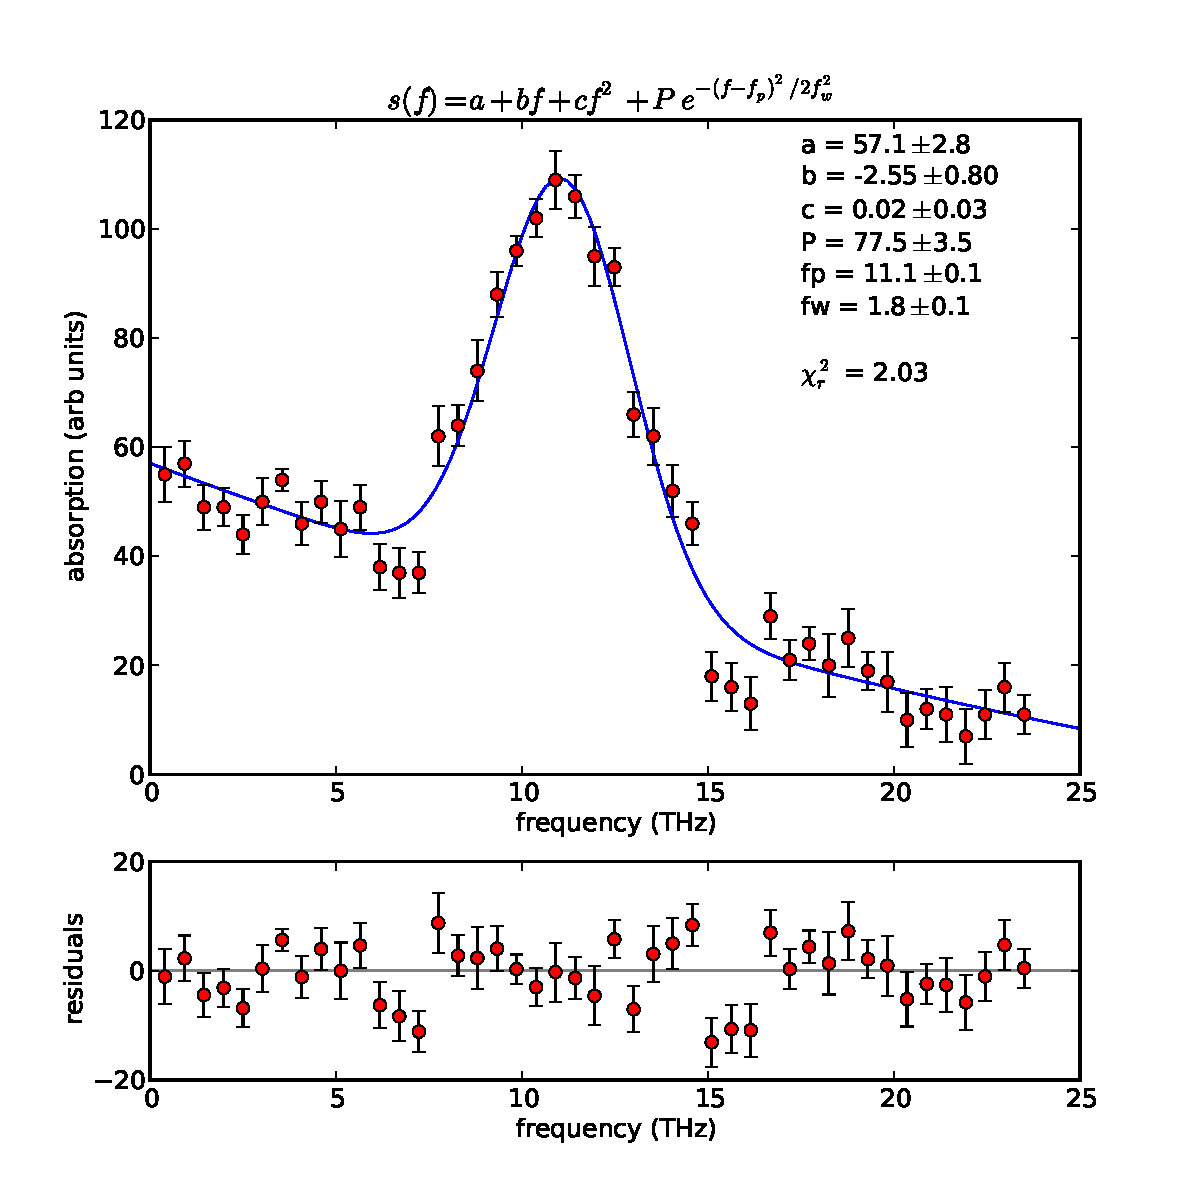
\includegraphics{FitSpectrum.pdf}}
\caption{Fit to Gaussian with quadratic polynomial background.}\label{chap8/chap8_fitting:fig-fitspectrum}\end{figure}

Finally, we note that we have used the MatPlotLib package \code{gridspec} to create the two subplots with different heights.  The \code{gridspec} are made in lines 3 (where the package is imported), 36 (where 2 rows and 1 column are specified with relative heights of 6 to 2), 39 (where the first \code{gs{[}0{]}} height is specified), and 54 (where the second \code{gs{[}1{]}} height is specified).  More details about the \code{gridspec} package can be found at the MatPlotLib web site.
\newpage

\section{Exercises}
\label{chap8/chap8_fitting:exercises}\begin{enumerate}
\item {} 
When a voltage source is connected across a resistor and inductor in series, the voltage across the inductor \(V_i(t)\) is predicted to obey the equation
\phantomsection\label{chap8/chap8_fitting:equation-eq:inductorDecay}\begin{gather}
\begin{split}V(t) = V_0 e^{-\Gamma t}\end{split}\label{chap8/chap8_fitting-eq:inductorDecay}
\end{gather}
where \(t\) is the time and the decay rate \(\Gamma=R/L\) is the ratio of the  resistance \(R\) to the inductance \(L\) of the circuit.  In this problem, you are to write a Python routine that fits the above equation to the data below for the voltage measured across an inductor after it is connected in series with a resistor to a voltage source.  Following the example in the text, linearize the \eqref{chap8/chap8_fitting-eq:inductorDecay} and use a linear fitting routine, either the one you wrote from the previous chapter or one from NumPy or SciPy.
\begin{enumerate}
\item {} 
Find the best values of \(\Gamma\) and \(V_0\) and the uncertainties in their values \(\sigma_\Gamma\) and \(\sigma_{V_0}\).

\item {} 
Find the value of \(\chi_r^2\) for your fit.  Does it make sense?

\item {} 
Make a semi-log plot of the data using symbols with error bars (no line) and of the fit (line only).  The fit should appear as a straight line that goes through the data points.

\item {} 
If the resistor has a value of 10.0 \(\mathrm{k}\Omega\), what is the value of the inductance and its uncertainty according to your fit, assuming that the error in the resistance is negligibly small.

\begin{Verbatim}[commandchars=\\\{\},numbers=left,firstnumber=1,stepnumber=1]
Data for decay of voltage across an inductor
in an RL circuit
Date: 24\PYGZhy{}Oct\PYGZhy{}2012
Data taken by D. M. Blantogg and T. P. Chaitor

time (ns)   voltage (volts)  uncertainty (volts)
    0.0        5.08e+00        1.12e\PYGZhy{}01
   32.8        3.29e+00        9.04e\PYGZhy{}02
   65.6        2.23e+00        7.43e\PYGZhy{}02
   98.4        1.48e+00        6.05e\PYGZhy{}02
  131.2        1.11e+00        5.25e\PYGZhy{}02
  164.0        6.44e\PYGZhy{}01        4.00e\PYGZhy{}02
  196.8        4.76e\PYGZhy{}01        3.43e\PYGZhy{}02
  229.6        2.73e\PYGZhy{}01        2.60e\PYGZhy{}02
  262.4        1.88e\PYGZhy{}01        2.16e\PYGZhy{}02
  295.2        1.41e\PYGZhy{}01        1.87e\PYGZhy{}02
  328.0        9.42e\PYGZhy{}02        1.53e\PYGZhy{}02
  360.8        7.68e\PYGZhy{}02        1.38e\PYGZhy{}02
  393.6        3.22e\PYGZhy{}02        8.94e\PYGZhy{}03
  426.4        3.22e\PYGZhy{}02        8.94e\PYGZhy{}03
  459.2        1.98e\PYGZhy{}02        7.01e\PYGZhy{}03
  492.0        1.98e\PYGZhy{}02        7.01e\PYGZhy{}03
\end{Verbatim}

\end{enumerate}

\item {} 
Small nanoparticles of soot suspended in water start to aggregate when salt is added.  The average radius \(r\) of the aggregates is predicted to grow as a power law in time \(t\) according to the equation \(r = r_0t^n\).  Taking the logarithm of this equation gives \(\ln r = n\ln t + \ln r_0\).  Thus the data should fall on a straight line if \(\ln r\) is plotted \emph{vs} \(\ln t\).
\begin{enumerate}
\item {} 
Plot the data below on a graph of \(\ln r\) \emph{vs} \(\ln t\) to see if the data fall approximately on a straight line.

\begin{Verbatim}[commandchars=\\\{\},numbers=left,firstnumber=1,stepnumber=1]
Size of growing aggregate
Date: 19\PYGZhy{}Nov\PYGZhy{}2013
Data taken by M. D. Gryart and M. L. Waites
time (m)   size (nm)    unc (nm)
  0.12        115         10
  0.18        130         12
  0.42        202         14
  0.90        335         18
  2.10        510         20
  6.00        890         30
 18.00       1700         40
 42.00       2600         50
\end{Verbatim}

\item {} 
Defining \(y = \ln r\) and \(x = \ln t\), use the linear fitting routine you wrote for the previous problem to fit the data and find the optimal values for the slope and \(y\) intercept, as well as their uncertainties.  Use these fitted values to find the optimal values of the the amplitude \(r_0\) and the power \(n\) in the fitting function \(r = r_0t^n\).  What are the fitted values of \(r_0\) and \(n\)?  What is the value of \(\chi_r^2\)?  Does a power law provide an adequate model for the data?

\end{enumerate}

\item {} 
In this problem you explore using a non-linear least square fitting routine to fit the data shown in the figure below.   The data, including the uncertainties in the \(y\) values, are provided in the table below.  Your task is to fit the function
\phantomsection\label{chap8/chap8_fitting:equation-eq:OscDecay}\begin{gather}
\begin{split}d(t) = A (1+B\,\cos\omega t) e^{-t^2/2\tau^2} + C\end{split}\label{chap8/chap8_fitting-eq:OscDecay}
\end{gather}
to the data, where the fitting parameters are \(A\), \(B\), \(C\), \(\omega\), and \(\tau\).
\begin{figure}[htbp]
\centering

\scalebox{0.800000}{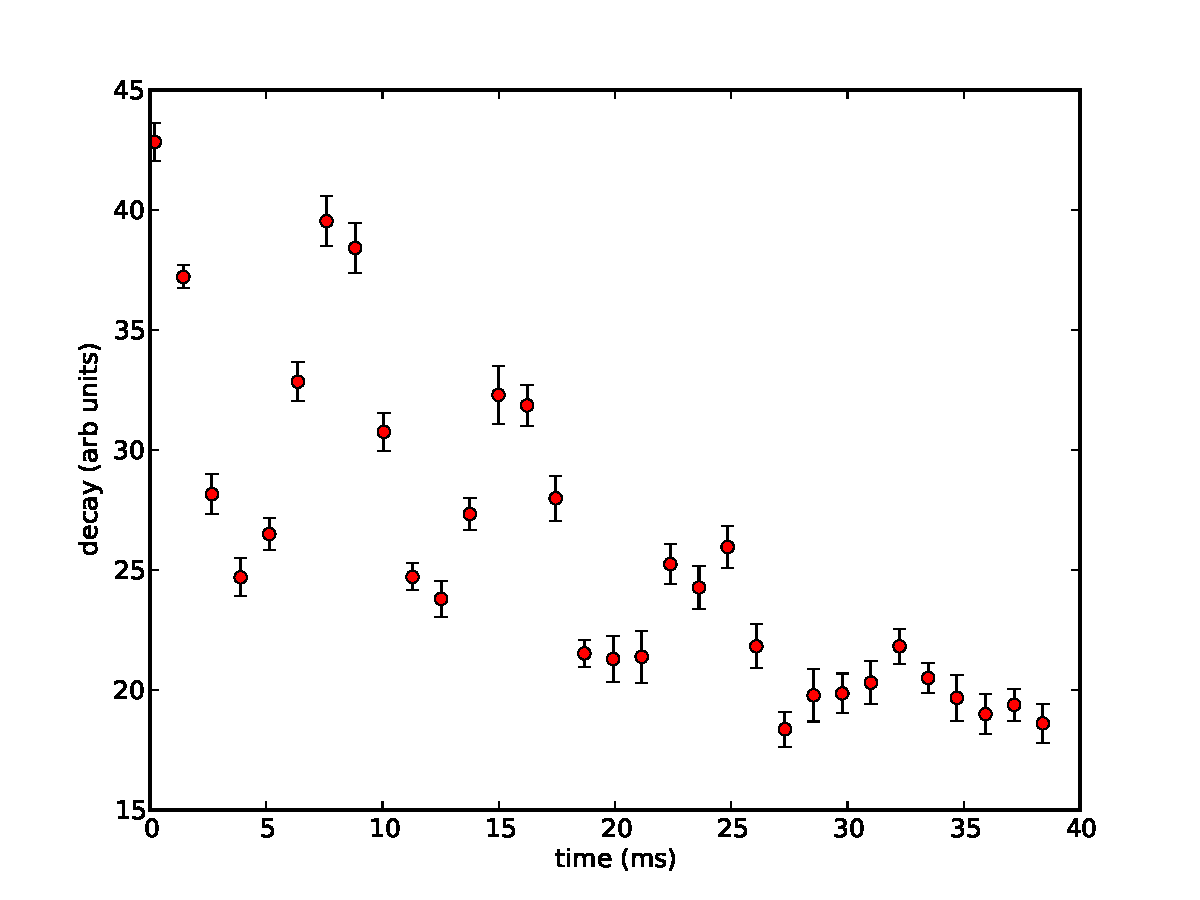
\includegraphics{DataOscDecay.pdf}}
\label{chap8/chap8_fitting:fig-oscdata}\end{figure}
\begin{enumerate}
\item {} 
Write a Python program that (\emph{i}) reads the data in from a data file, (\emph{ii}) defines a function \code{oscDecay(t, A, B, C, tau, omega)} for the function \(d(t)\) above, and (\emph{iii}) produces a plot of the data and the function \(d(t)\).  Choose the fitting parameters  \code{A}, \code{B}, \code{C}, \code{tau}, and \code{omega} to produce an approximate fit ``by eye'' to the data.  You should be able estimate reasonable values for these parameters just by looking at the data and thinking about the behavior of \(d(t)\).  For example, \(d(0)=A(1+B)+C\) while \(d(\infty)=C\).  What parameter in \(d(t)\) controls the period of the peaks observed in the data?  Use that information to estimate the value of that parameter.

\item {} 
Following the example in section {\hyperref[chap8/chap8_fitting:sec-nonlinfit]{\emph{Nonlinear fitting}}}, write a program using the SciPy function \code{scipy.optimize.curve\_fit} to fit Eq. \eqref{chap8/chap8_fitting-eq:OscDecay} to the data and thus find the optimal values of the fitting parameters \(A\), \(B\), \(C\), \(\omega\), and \(\tau\).  Your program should plot the data along with the fitting function using the optimal values of the fitting parameters.  Write a function to calculate the reduced \(\chi^2\).  Print out the value of the reduced \(\chi^2\) on your plot along with the optimal values of the fitting parameters.  You can use the results from part (a) to estimate good starting values of the fitting parameters

\item {} 
Once you have found the optimal fitting parameters, run your fitting program again using for starting values the optimal values of the fitting parameters \(A\), \(B\), \(C\), and \(\tau\), but set the starting value of \(\omega\) to be 3 times the optimal value.  You should find that the program converges to a different set of fitting parameters than the ones you found in part (b).  Using the program you wrote for part (b) make a plot of the data and the fit like the one you did for part (a).  The fit should be noticeably worse.  What is the value of the reduced \(\chi^2\) for this fit; it should be much larger than the one you found for part (c).  The program  has found a local minimum in \(\chi^2\)---one that is obviously is not the best fit!

\item {} 
Setting the fitting parameters \(A\), \(B\), \(C\), and \(\tau\) to the optimal values you found in part (b), plot \(\chi_r^2\) as a function of \(\omega\) for \(\omega\) spanning the range from 0.05 to 3.95.  You should observe several local minima for different values of \(\chi_r^2\); the global minimum in \(\chi_r^2\) should occur for the optimal value of \(\omega\) you found in part (b).

\begin{Verbatim}[commandchars=\\\{\},numbers=left,firstnumber=1,stepnumber=1]
Data for absorption spectrum
Date: 21\PYGZhy{}Nov\PYGZhy{}2012
Data taken by P. Dubson and M. Sparks
time (ms)  signal  uncertainty
  0.2      41.1       0.9
  1.4      37.2       0.9
  2.7      28.3       0.9
  3.9      24.8       1.1
  5.1      27.8       0.8
  6.4      34.5       0.7
  7.6      39.0       0.9
  8.8      37.7       0.8
 10.1      29.8       0.9
 11.3      22.2       0.7
 12.5      22.3       0.6
 13.8      26.7       1.1
 15.0      30.4       0.7
 16.2      32.6       0.8
 17.5      28.9       0.8
 18.7      22.9       1.3
 19.9      21.7       0.9
 21.1      22.1       1.0
 22.4      22.3       1.0
 23.6      26.3       1.0
 24.8      26.2       0.8
 26.1      21.4       0.9
 27.3      20.0       1.0
 28.5      20.1       1.2
 29.8      21.2       0.5
 31.0      22.0       0.9
 32.2      21.6       0.7
 33.5      21.0       0.7
 34.7      19.7       0.9
 35.9      17.9       0.9
 37.2      18.1       0.8
 38.4      18.9       1.1
\end{Verbatim}

\end{enumerate}

\end{enumerate}


\chapter{Numerical Routines: SciPy and NumPy}
\label{chap9/chap9_scipy::doc}\label{chap9/chap9_scipy:numerical-routines-scipy-and-numpy}\label{chap9/chap9_scipy:chap9}
SciPy is a Python library of mathematical routines.  Many of the SciPy routines are Python ``wrappers'', that is, Python routines that provide a Python interface for numerical libraries and routines originally written in Fortran, C, or C++.  Thus, SciPy lets you take advantage of the decades of work that has gone into creating and optimizing numerical routines for science and engineering.  Because the Fortran, C, or C++ code that Python accesses is compiled, these routines typically run very fast.  Therefore, there is no real downside---no speed penalty---for using Python in these cases.

We have already encountered one of SciPy's routines, \code{scipy.optimize.leastsq}, for fitting nonlinear functions to experimental data, which was introduced in the the chapter on {\hyperref[chap8/chap8_fitting:chap8]{\emph{Curve Fitting}}}.   Here we will provide a further introduction to a number of other SciPy packages, in particular those on special functions, numerical integration, including routines for numerically solving ordinary differential equations (ODEs), discrete Fourier transforms, linear algebra, and solving non-linear equations.  Our introduction to these capabilities does not include extensive background on the numerical methods employed; that is a topic for another text.  Here we simply introduce the SciPy routines for performing some of the more frequently required numerical tasks.

One final note:  SciPy makes extensive use of NumPy arrays, so NumPy should always be imported with SciPy

\index{special functions}

\section{Special functions}
\label{chap9/chap9_scipy:index-0}\label{chap9/chap9_scipy:specfunc}\label{chap9/chap9_scipy:special-functions}
SciPy provides a plethora of special functions, including Bessel functions (and routines for finding their zeros, derivatives, and integrals), error functions, the gamma function, Legendre, Laguerre, and Hermite polynomials (and other polynomial functions), Mathieu functions, many statistical functions, and a number of other functions.  Most are contained in the \code{scipy.special} library, and each has its own special arguments and syntax, depending on the vagaries of the particular function.  We demonstrate a number of them in the code below that produces a plot of the different functions called.  For more information, you should consult the SciPy web site on the \code{scipy.special} library.
\begin{quote}
\begin{figure}[htbp]
\centering
\capstart

\scalebox{1.000000}{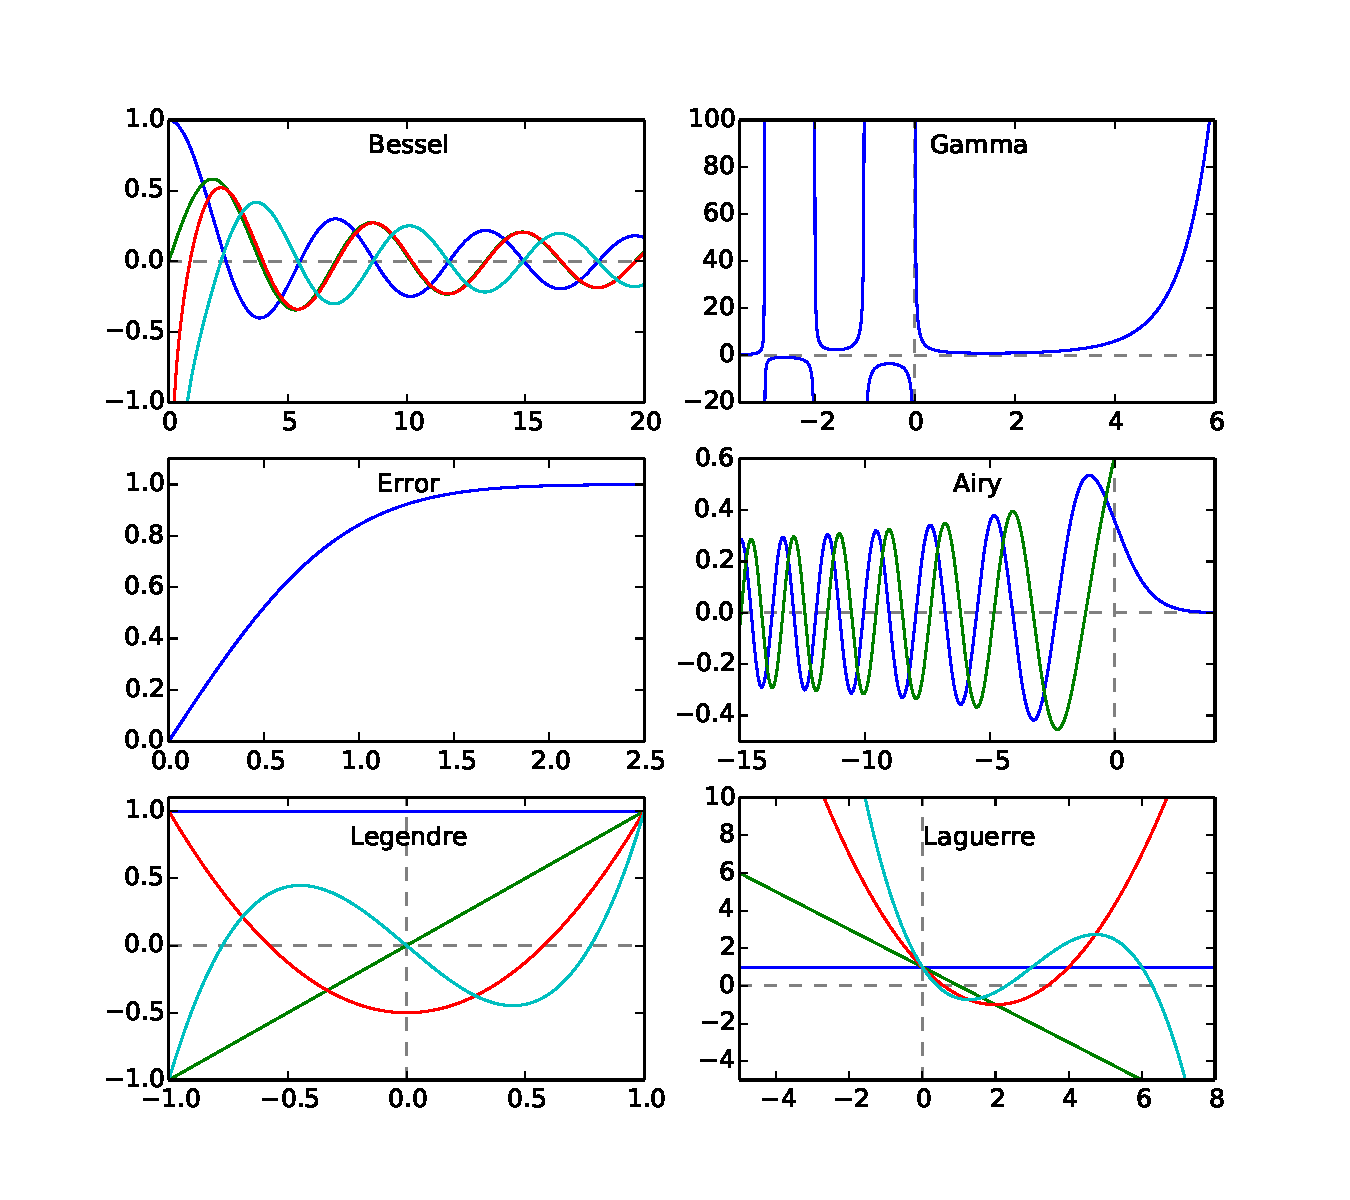
\includegraphics{specFuncPlots.pdf}}
\caption{Plots of a few selected special functions}\label{chap9/chap9_scipy:fig-specfuncplots}\end{figure}
\end{quote}

\begin{Verbatim}[commandchars=\\\{\},numbers=left,firstnumber=1,stepnumber=1]
    \PYG{k+kn}{import} \PYG{n+nn}{numpy} \PYG{k+kn}{as} \PYG{n+nn}{np}
    \PYG{k+kn}{import} \PYG{n+nn}{scipy.special}
    \PYG{k+kn}{import} \PYG{n+nn}{matplotlib.pyplot} \PYG{k+kn}{as} \PYG{n+nn}{plt}

    \PYG{c}{\PYGZsh{} create a figure window}
    \PYG{n}{fig} \PYG{o}{=} \PYG{n}{plt}\PYG{o}{.}\PYG{n}{figure}\PYG{p}{(}\PYG{l+m+mi}{1}\PYG{p}{,} \PYG{n}{figsize}\PYG{o}{=}\PYG{p}{(}\PYG{l+m+mi}{9}\PYG{p}{,}\PYG{l+m+mi}{8}\PYG{p}{)}\PYG{p}{)}

    \PYG{c}{\PYGZsh{} create arrays for a few Bessel functions and plot them}
    \PYG{n}{x} \PYG{o}{=} \PYG{n}{np}\PYG{o}{.}\PYG{n}{linspace}\PYG{p}{(}\PYG{l+m+mi}{0}\PYG{p}{,} \PYG{l+m+mi}{20}\PYG{p}{,} \PYG{l+m+mi}{256}\PYG{p}{)}
    \PYG{n}{j0} \PYG{o}{=} \PYG{n}{scipy}\PYG{o}{.}\PYG{n}{special}\PYG{o}{.}\PYG{n}{jn}\PYG{p}{(}\PYG{l+m+mi}{0}\PYG{p}{,} \PYG{n}{x}\PYG{p}{)}
    \PYG{n}{j1} \PYG{o}{=} \PYG{n}{scipy}\PYG{o}{.}\PYG{n}{special}\PYG{o}{.}\PYG{n}{jn}\PYG{p}{(}\PYG{l+m+mi}{1}\PYG{p}{,} \PYG{n}{x}\PYG{p}{)}
    \PYG{n}{y0} \PYG{o}{=} \PYG{n}{scipy}\PYG{o}{.}\PYG{n}{special}\PYG{o}{.}\PYG{n}{yn}\PYG{p}{(}\PYG{l+m+mi}{0}\PYG{p}{,} \PYG{n}{x}\PYG{p}{)}
    \PYG{n}{y1} \PYG{o}{=} \PYG{n}{scipy}\PYG{o}{.}\PYG{n}{special}\PYG{o}{.}\PYG{n}{yn}\PYG{p}{(}\PYG{l+m+mi}{1}\PYG{p}{,} \PYG{n}{x}\PYG{p}{)}
    \PYG{n}{ax1} \PYG{o}{=} \PYG{n}{fig}\PYG{o}{.}\PYG{n}{add\PYGZus{}subplot}\PYG{p}{(}\PYG{l+m+mi}{321}\PYG{p}{)}
    \PYG{n}{ax1}\PYG{o}{.}\PYG{n}{plot}\PYG{p}{(}\PYG{n}{x}\PYG{p}{,}\PYG{n}{j0}\PYG{p}{,} \PYG{n}{x}\PYG{p}{,}\PYG{n}{j1}\PYG{p}{,} \PYG{n}{x}\PYG{p}{,}\PYG{n}{y0}\PYG{p}{,} \PYG{n}{x}\PYG{p}{,}\PYG{n}{y1}\PYG{p}{)}
    \PYG{n}{ax1}\PYG{o}{.}\PYG{n}{axhline}\PYG{p}{(}\PYG{n}{color}\PYG{o}{=}\PYG{l+s}{\PYGZdq{}}\PYG{l+s}{grey}\PYG{l+s}{\PYGZdq{}}\PYG{p}{,} \PYG{n}{ls}\PYG{o}{=}\PYG{l+s}{\PYGZdq{}}\PYG{l+s}{\PYGZhy{}\PYGZhy{}}\PYG{l+s}{\PYGZdq{}}\PYG{p}{,} \PYG{n}{zorder}\PYG{o}{=}\PYG{o}{\PYGZhy{}}\PYG{l+m+mi}{1}\PYG{p}{)}
    \PYG{n}{ax1}\PYG{o}{.}\PYG{n}{set\PYGZus{}ylim}\PYG{p}{(}\PYG{o}{\PYGZhy{}}\PYG{l+m+mi}{1}\PYG{p}{,}\PYG{l+m+mi}{1}\PYG{p}{)}
    \PYG{n}{ax1}\PYG{o}{.}\PYG{n}{text}\PYG{p}{(}\PYG{l+m+mf}{0.5}\PYG{p}{,} \PYG{l+m+mf}{0.95}\PYG{p}{,}\PYG{l+s}{\PYGZsq{}}\PYG{l+s}{Bessel}\PYG{l+s}{\PYGZsq{}}\PYG{p}{,} \PYG{n}{ha}\PYG{o}{=}\PYG{l+s}{\PYGZsq{}}\PYG{l+s}{center}\PYG{l+s}{\PYGZsq{}}\PYG{p}{,} \PYG{n}{va}\PYG{o}{=}\PYG{l+s}{\PYGZsq{}}\PYG{l+s}{top}\PYG{l+s}{\PYGZsq{}}\PYG{p}{,}
         \PYG{n}{transform} \PYG{o}{=} \PYG{n}{ax1}\PYG{o}{.}\PYG{n}{transAxes}\PYG{p}{)}

    \PYG{c}{\PYGZsh{} gamma function}
    \PYG{n}{x} \PYG{o}{=} \PYG{n}{np}\PYG{o}{.}\PYG{n}{linspace}\PYG{p}{(}\PYG{o}{\PYGZhy{}}\PYG{l+m+mf}{3.5}\PYG{p}{,} \PYG{l+m+mf}{6.}\PYG{p}{,} \PYG{l+m+mi}{3601}\PYG{p}{)}
    \PYG{n}{g} \PYG{o}{=} \PYG{n}{scipy}\PYG{o}{.}\PYG{n}{special}\PYG{o}{.}\PYG{n}{gamma}\PYG{p}{(}\PYG{n}{x}\PYG{p}{)}
    \PYG{n}{g} \PYG{o}{=} \PYG{n}{np}\PYG{o}{.}\PYG{n}{ma}\PYG{o}{.}\PYG{n}{masked\PYGZus{}outside}\PYG{p}{(}\PYG{n}{g}\PYG{p}{,} \PYG{o}{\PYGZhy{}}\PYG{l+m+mi}{100}\PYG{p}{,} \PYG{l+m+mi}{400}\PYG{p}{)}
    \PYG{n}{ax2} \PYG{o}{=} \PYG{n}{fig}\PYG{o}{.}\PYG{n}{add\PYGZus{}subplot}\PYG{p}{(}\PYG{l+m+mi}{322}\PYG{p}{)}
    \PYG{n}{ax2}\PYG{o}{.}\PYG{n}{plot}\PYG{p}{(}\PYG{n}{x}\PYG{p}{,}\PYG{n}{g}\PYG{p}{)}
    \PYG{n}{ax2}\PYG{o}{.}\PYG{n}{set\PYGZus{}xlim}\PYG{p}{(}\PYG{o}{\PYGZhy{}}\PYG{l+m+mf}{3.5}\PYG{p}{,} \PYG{l+m+mi}{6}\PYG{p}{)}
    \PYG{n}{ax2}\PYG{o}{.}\PYG{n}{axhline}\PYG{p}{(}\PYG{n}{color}\PYG{o}{=}\PYG{l+s}{\PYGZdq{}}\PYG{l+s}{grey}\PYG{l+s}{\PYGZdq{}}\PYG{p}{,} \PYG{n}{ls}\PYG{o}{=}\PYG{l+s}{\PYGZdq{}}\PYG{l+s}{\PYGZhy{}\PYGZhy{}}\PYG{l+s}{\PYGZdq{}}\PYG{p}{,} \PYG{n}{zorder}\PYG{o}{=}\PYG{o}{\PYGZhy{}}\PYG{l+m+mi}{1}\PYG{p}{)}
    \PYG{n}{ax2}\PYG{o}{.}\PYG{n}{axvline}\PYG{p}{(}\PYG{n}{color}\PYG{o}{=}\PYG{l+s}{\PYGZdq{}}\PYG{l+s}{grey}\PYG{l+s}{\PYGZdq{}}\PYG{p}{,} \PYG{n}{ls}\PYG{o}{=}\PYG{l+s}{\PYGZdq{}}\PYG{l+s}{\PYGZhy{}\PYGZhy{}}\PYG{l+s}{\PYGZdq{}}\PYG{p}{,} \PYG{n}{zorder}\PYG{o}{=}\PYG{o}{\PYGZhy{}}\PYG{l+m+mi}{1}\PYG{p}{)}
    \PYG{n}{ax2}\PYG{o}{.}\PYG{n}{set\PYGZus{}ylim}\PYG{p}{(}\PYG{o}{\PYGZhy{}}\PYG{l+m+mi}{20}\PYG{p}{,} \PYG{l+m+mi}{100}\PYG{p}{)}
    \PYG{n}{ax2}\PYG{o}{.}\PYG{n}{text}\PYG{p}{(}\PYG{l+m+mf}{0.5}\PYG{p}{,} \PYG{l+m+mf}{0.95}\PYG{p}{,}\PYG{l+s}{\PYGZsq{}}\PYG{l+s}{Gamma}\PYG{l+s}{\PYGZsq{}}\PYG{p}{,} \PYG{n}{ha}\PYG{o}{=}\PYG{l+s}{\PYGZsq{}}\PYG{l+s}{center}\PYG{l+s}{\PYGZsq{}}\PYG{p}{,} \PYG{n}{va}\PYG{o}{=}\PYG{l+s}{\PYGZsq{}}\PYG{l+s}{top}\PYG{l+s}{\PYGZsq{}}\PYG{p}{,}
         \PYG{n}{transform} \PYG{o}{=} \PYG{n}{ax2}\PYG{o}{.}\PYG{n}{transAxes}\PYG{p}{)}

    \PYG{c}{\PYGZsh{} error function}
    \PYG{n}{x} \PYG{o}{=} \PYG{n}{np}\PYG{o}{.}\PYG{n}{linspace}\PYG{p}{(}\PYG{l+m+mi}{0}\PYG{p}{,} \PYG{l+m+mf}{2.5}\PYG{p}{,} \PYG{l+m+mi}{256}\PYG{p}{)}
    \PYG{n}{ef} \PYG{o}{=} \PYG{n}{scipy}\PYG{o}{.}\PYG{n}{special}\PYG{o}{.}\PYG{n}{erf}\PYG{p}{(}\PYG{n}{x}\PYG{p}{)}
    \PYG{n}{ax3} \PYG{o}{=} \PYG{n}{fig}\PYG{o}{.}\PYG{n}{add\PYGZus{}subplot}\PYG{p}{(}\PYG{l+m+mi}{323}\PYG{p}{)}
    \PYG{n}{ax3}\PYG{o}{.}\PYG{n}{plot}\PYG{p}{(}\PYG{n}{x}\PYG{p}{,}\PYG{n}{ef}\PYG{p}{)}
    \PYG{n}{ax3}\PYG{o}{.}\PYG{n}{set\PYGZus{}ylim}\PYG{p}{(}\PYG{l+m+mi}{0}\PYG{p}{,}\PYG{l+m+mf}{1.1}\PYG{p}{)}
    \PYG{n}{ax3}\PYG{o}{.}\PYG{n}{text}\PYG{p}{(}\PYG{l+m+mf}{0.5}\PYG{p}{,} \PYG{l+m+mf}{0.95}\PYG{p}{,}\PYG{l+s}{\PYGZsq{}}\PYG{l+s}{Error}\PYG{l+s}{\PYGZsq{}}\PYG{p}{,} \PYG{n}{ha}\PYG{o}{=}\PYG{l+s}{\PYGZsq{}}\PYG{l+s}{center}\PYG{l+s}{\PYGZsq{}}\PYG{p}{,} \PYG{n}{va}\PYG{o}{=}\PYG{l+s}{\PYGZsq{}}\PYG{l+s}{top}\PYG{l+s}{\PYGZsq{}}\PYG{p}{,}
         \PYG{n}{transform} \PYG{o}{=} \PYG{n}{ax3}\PYG{o}{.}\PYG{n}{transAxes}\PYG{p}{)}

    \PYG{c}{\PYGZsh{} Airy function}
    \PYG{n}{x} \PYG{o}{=} \PYG{n}{np}\PYG{o}{.}\PYG{n}{linspace}\PYG{p}{(}\PYG{o}{\PYGZhy{}}\PYG{l+m+mi}{15}\PYG{p}{,} \PYG{l+m+mi}{4}\PYG{p}{,} \PYG{l+m+mi}{256}\PYG{p}{)}
    \PYG{n}{ai}\PYG{p}{,} \PYG{n}{aip}\PYG{p}{,} \PYG{n}{bi}\PYG{p}{,} \PYG{n}{bip} \PYG{o}{=} \PYG{n}{scipy}\PYG{o}{.}\PYG{n}{special}\PYG{o}{.}\PYG{n}{airy}\PYG{p}{(}\PYG{n}{x}\PYG{p}{)}
    \PYG{n}{ax4} \PYG{o}{=} \PYG{n}{fig}\PYG{o}{.}\PYG{n}{add\PYGZus{}subplot}\PYG{p}{(}\PYG{l+m+mi}{324}\PYG{p}{)}
    \PYG{n}{ax4}\PYG{o}{.}\PYG{n}{plot}\PYG{p}{(}\PYG{n}{x}\PYG{p}{,}\PYG{n}{ai}\PYG{p}{,} \PYG{n}{x}\PYG{p}{,}\PYG{n}{bi}\PYG{p}{)}
    \PYG{n}{ax4}\PYG{o}{.}\PYG{n}{axhline}\PYG{p}{(}\PYG{n}{color}\PYG{o}{=}\PYG{l+s}{\PYGZdq{}}\PYG{l+s}{grey}\PYG{l+s}{\PYGZdq{}}\PYG{p}{,} \PYG{n}{ls}\PYG{o}{=}\PYG{l+s}{\PYGZdq{}}\PYG{l+s}{\PYGZhy{}\PYGZhy{}}\PYG{l+s}{\PYGZdq{}}\PYG{p}{,} \PYG{n}{zorder}\PYG{o}{=}\PYG{o}{\PYGZhy{}}\PYG{l+m+mi}{1}\PYG{p}{)}
    \PYG{n}{ax4}\PYG{o}{.}\PYG{n}{axvline}\PYG{p}{(}\PYG{n}{color}\PYG{o}{=}\PYG{l+s}{\PYGZdq{}}\PYG{l+s}{grey}\PYG{l+s}{\PYGZdq{}}\PYG{p}{,} \PYG{n}{ls}\PYG{o}{=}\PYG{l+s}{\PYGZdq{}}\PYG{l+s}{\PYGZhy{}\PYGZhy{}}\PYG{l+s}{\PYGZdq{}}\PYG{p}{,} \PYG{n}{zorder}\PYG{o}{=}\PYG{o}{\PYGZhy{}}\PYG{l+m+mi}{1}\PYG{p}{)}
    \PYG{n}{ax4}\PYG{o}{.}\PYG{n}{set\PYGZus{}xlim}\PYG{p}{(}\PYG{o}{\PYGZhy{}}\PYG{l+m+mi}{15}\PYG{p}{,}\PYG{l+m+mi}{4}\PYG{p}{)}
    \PYG{n}{ax4}\PYG{o}{.}\PYG{n}{set\PYGZus{}ylim}\PYG{p}{(}\PYG{o}{\PYGZhy{}}\PYG{l+m+mf}{0.5}\PYG{p}{,}\PYG{l+m+mf}{0.6}\PYG{p}{)}
    \PYG{n}{ax4}\PYG{o}{.}\PYG{n}{text}\PYG{p}{(}\PYG{l+m+mf}{0.5}\PYG{p}{,} \PYG{l+m+mf}{0.95}\PYG{p}{,}\PYG{l+s}{\PYGZsq{}}\PYG{l+s}{Airy}\PYG{l+s}{\PYGZsq{}}\PYG{p}{,} \PYG{n}{ha}\PYG{o}{=}\PYG{l+s}{\PYGZsq{}}\PYG{l+s}{center}\PYG{l+s}{\PYGZsq{}}\PYG{p}{,} \PYG{n}{va}\PYG{o}{=}\PYG{l+s}{\PYGZsq{}}\PYG{l+s}{top}\PYG{l+s}{\PYGZsq{}}\PYG{p}{,}
         \PYG{n}{transform} \PYG{o}{=} \PYG{n}{ax4}\PYG{o}{.}\PYG{n}{transAxes}\PYG{p}{)}

    \PYG{c}{\PYGZsh{} Legendre polynomials}
    \PYG{n}{x} \PYG{o}{=} \PYG{n}{np}\PYG{o}{.}\PYG{n}{linspace}\PYG{p}{(}\PYG{o}{\PYGZhy{}}\PYG{l+m+mi}{1}\PYG{p}{,} \PYG{l+m+mi}{1}\PYG{p}{,} \PYG{l+m+mi}{256}\PYG{p}{)}
    \PYG{n}{lp0} \PYG{o}{=} \PYG{n}{np}\PYG{o}{.}\PYG{n}{polyval}\PYG{p}{(}\PYG{n}{scipy}\PYG{o}{.}\PYG{n}{special}\PYG{o}{.}\PYG{n}{legendre}\PYG{p}{(}\PYG{l+m+mi}{0}\PYG{p}{)}\PYG{p}{,}\PYG{n}{x}\PYG{p}{)}
    \PYG{n}{lp1} \PYG{o}{=} \PYG{n}{np}\PYG{o}{.}\PYG{n}{polyval}\PYG{p}{(}\PYG{n}{scipy}\PYG{o}{.}\PYG{n}{special}\PYG{o}{.}\PYG{n}{legendre}\PYG{p}{(}\PYG{l+m+mi}{1}\PYG{p}{)}\PYG{p}{,}\PYG{n}{x}\PYG{p}{)}
    \PYG{n}{lp2} \PYG{o}{=} \PYG{n}{np}\PYG{o}{.}\PYG{n}{polyval}\PYG{p}{(}\PYG{n}{scipy}\PYG{o}{.}\PYG{n}{special}\PYG{o}{.}\PYG{n}{legendre}\PYG{p}{(}\PYG{l+m+mi}{2}\PYG{p}{)}\PYG{p}{,}\PYG{n}{x}\PYG{p}{)}
    \PYG{n}{lp3} \PYG{o}{=} \PYG{n}{np}\PYG{o}{.}\PYG{n}{polyval}\PYG{p}{(}\PYG{n}{scipy}\PYG{o}{.}\PYG{n}{special}\PYG{o}{.}\PYG{n}{legendre}\PYG{p}{(}\PYG{l+m+mi}{3}\PYG{p}{)}\PYG{p}{,}\PYG{n}{x}\PYG{p}{)}
    \PYG{n}{ax5} \PYG{o}{=} \PYG{n}{fig}\PYG{o}{.}\PYG{n}{add\PYGZus{}subplot}\PYG{p}{(}\PYG{l+m+mi}{325}\PYG{p}{)}
    \PYG{n}{ax5}\PYG{o}{.}\PYG{n}{plot}\PYG{p}{(}\PYG{n}{x}\PYG{p}{,}\PYG{n}{lp0}\PYG{p}{,} \PYG{n}{x}\PYG{p}{,}\PYG{n}{lp1}\PYG{p}{,} \PYG{n}{x}\PYG{p}{,}\PYG{n}{lp2}\PYG{p}{,} \PYG{n}{x}\PYG{p}{,}\PYG{n}{lp3}\PYG{p}{)}
    \PYG{n}{ax5}\PYG{o}{.}\PYG{n}{axhline}\PYG{p}{(}\PYG{n}{color}\PYG{o}{=}\PYG{l+s}{\PYGZdq{}}\PYG{l+s}{grey}\PYG{l+s}{\PYGZdq{}}\PYG{p}{,} \PYG{n}{ls}\PYG{o}{=}\PYG{l+s}{\PYGZdq{}}\PYG{l+s}{\PYGZhy{}\PYGZhy{}}\PYG{l+s}{\PYGZdq{}}\PYG{p}{,} \PYG{n}{zorder}\PYG{o}{=}\PYG{o}{\PYGZhy{}}\PYG{l+m+mi}{1}\PYG{p}{)}
    \PYG{n}{ax5}\PYG{o}{.}\PYG{n}{axvline}\PYG{p}{(}\PYG{n}{color}\PYG{o}{=}\PYG{l+s}{\PYGZdq{}}\PYG{l+s}{grey}\PYG{l+s}{\PYGZdq{}}\PYG{p}{,} \PYG{n}{ls}\PYG{o}{=}\PYG{l+s}{\PYGZdq{}}\PYG{l+s}{\PYGZhy{}\PYGZhy{}}\PYG{l+s}{\PYGZdq{}}\PYG{p}{,} \PYG{n}{zorder}\PYG{o}{=}\PYG{o}{\PYGZhy{}}\PYG{l+m+mi}{1}\PYG{p}{)}
    \PYG{n}{ax5}\PYG{o}{.}\PYG{n}{set\PYGZus{}ylim}\PYG{p}{(}\PYG{o}{\PYGZhy{}}\PYG{l+m+mi}{1}\PYG{p}{,}\PYG{l+m+mf}{1.1}\PYG{p}{)}
    \PYG{n}{ax5}\PYG{o}{.}\PYG{n}{text}\PYG{p}{(}\PYG{l+m+mf}{0.5}\PYG{p}{,} \PYG{l+m+mf}{0.9}\PYG{p}{,}\PYG{l+s}{\PYGZsq{}}\PYG{l+s}{Legendre}\PYG{l+s}{\PYGZsq{}}\PYG{p}{,} \PYG{n}{ha}\PYG{o}{=}\PYG{l+s}{\PYGZsq{}}\PYG{l+s}{center}\PYG{l+s}{\PYGZsq{}}\PYG{p}{,} \PYG{n}{va}\PYG{o}{=}\PYG{l+s}{\PYGZsq{}}\PYG{l+s}{top}\PYG{l+s}{\PYGZsq{}}\PYG{p}{,}
         \PYG{n}{transform} \PYG{o}{=} \PYG{n}{ax5}\PYG{o}{.}\PYG{n}{transAxes}\PYG{p}{)}

    \PYG{c}{\PYGZsh{} Laguerre polynomials}
    \PYG{n}{x} \PYG{o}{=} \PYG{n}{np}\PYG{o}{.}\PYG{n}{linspace}\PYG{p}{(}\PYG{o}{\PYGZhy{}}\PYG{l+m+mi}{5}\PYG{p}{,} \PYG{l+m+mi}{8}\PYG{p}{,} \PYG{l+m+mi}{256}\PYG{p}{)}
    \PYG{n}{lg0} \PYG{o}{=} \PYG{n}{np}\PYG{o}{.}\PYG{n}{polyval}\PYG{p}{(}\PYG{n}{scipy}\PYG{o}{.}\PYG{n}{special}\PYG{o}{.}\PYG{n}{laguerre}\PYG{p}{(}\PYG{l+m+mi}{0}\PYG{p}{)}\PYG{p}{,}\PYG{n}{x}\PYG{p}{)}
    \PYG{n}{lg1} \PYG{o}{=} \PYG{n}{np}\PYG{o}{.}\PYG{n}{polyval}\PYG{p}{(}\PYG{n}{scipy}\PYG{o}{.}\PYG{n}{special}\PYG{o}{.}\PYG{n}{laguerre}\PYG{p}{(}\PYG{l+m+mi}{1}\PYG{p}{)}\PYG{p}{,}\PYG{n}{x}\PYG{p}{)}
    \PYG{n}{lg2} \PYG{o}{=} \PYG{n}{np}\PYG{o}{.}\PYG{n}{polyval}\PYG{p}{(}\PYG{n}{scipy}\PYG{o}{.}\PYG{n}{special}\PYG{o}{.}\PYG{n}{laguerre}\PYG{p}{(}\PYG{l+m+mi}{2}\PYG{p}{)}\PYG{p}{,}\PYG{n}{x}\PYG{p}{)}
    \PYG{n}{lg3} \PYG{o}{=} \PYG{n}{np}\PYG{o}{.}\PYG{n}{polyval}\PYG{p}{(}\PYG{n}{scipy}\PYG{o}{.}\PYG{n}{special}\PYG{o}{.}\PYG{n}{laguerre}\PYG{p}{(}\PYG{l+m+mi}{3}\PYG{p}{)}\PYG{p}{,}\PYG{n}{x}\PYG{p}{)}
    \PYG{n}{ax6} \PYG{o}{=} \PYG{n}{fig}\PYG{o}{.}\PYG{n}{add\PYGZus{}subplot}\PYG{p}{(}\PYG{l+m+mi}{326}\PYG{p}{)}
    \PYG{n}{ax6}\PYG{o}{.}\PYG{n}{plot}\PYG{p}{(}\PYG{n}{x}\PYG{p}{,}\PYG{n}{lg0}\PYG{p}{,} \PYG{n}{x}\PYG{p}{,}\PYG{n}{lg1}\PYG{p}{,} \PYG{n}{x}\PYG{p}{,}\PYG{n}{lg2}\PYG{p}{,} \PYG{n}{x}\PYG{p}{,}\PYG{n}{lg3}\PYG{p}{)}
    \PYG{n}{ax6}\PYG{o}{.}\PYG{n}{axhline}\PYG{p}{(}\PYG{n}{color}\PYG{o}{=}\PYG{l+s}{\PYGZdq{}}\PYG{l+s}{grey}\PYG{l+s}{\PYGZdq{}}\PYG{p}{,} \PYG{n}{ls}\PYG{o}{=}\PYG{l+s}{\PYGZdq{}}\PYG{l+s}{\PYGZhy{}\PYGZhy{}}\PYG{l+s}{\PYGZdq{}}\PYG{p}{,} \PYG{n}{zorder}\PYG{o}{=}\PYG{o}{\PYGZhy{}}\PYG{l+m+mi}{1}\PYG{p}{)}
    \PYG{n}{ax6}\PYG{o}{.}\PYG{n}{axvline}\PYG{p}{(}\PYG{n}{color}\PYG{o}{=}\PYG{l+s}{\PYGZdq{}}\PYG{l+s}{grey}\PYG{l+s}{\PYGZdq{}}\PYG{p}{,} \PYG{n}{ls}\PYG{o}{=}\PYG{l+s}{\PYGZdq{}}\PYG{l+s}{\PYGZhy{}\PYGZhy{}}\PYG{l+s}{\PYGZdq{}}\PYG{p}{,} \PYG{n}{zorder}\PYG{o}{=}\PYG{o}{\PYGZhy{}}\PYG{l+m+mi}{1}\PYG{p}{)}
    \PYG{n}{ax6}\PYG{o}{.}\PYG{n}{set\PYGZus{}xlim}\PYG{p}{(}\PYG{o}{\PYGZhy{}}\PYG{l+m+mi}{5}\PYG{p}{,}\PYG{l+m+mi}{8}\PYG{p}{)}
    \PYG{n}{ax6}\PYG{o}{.}\PYG{n}{set\PYGZus{}ylim}\PYG{p}{(}\PYG{o}{\PYGZhy{}}\PYG{l+m+mi}{5}\PYG{p}{,}\PYG{l+m+mi}{10}\PYG{p}{)}
    \PYG{n}{ax6}\PYG{o}{.}\PYG{n}{text}\PYG{p}{(}\PYG{l+m+mf}{0.5}\PYG{p}{,} \PYG{l+m+mf}{0.9}\PYG{p}{,}\PYG{l+s}{\PYGZsq{}}\PYG{l+s}{Laguerre}\PYG{l+s}{\PYGZsq{}}\PYG{p}{,} \PYG{n}{ha}\PYG{o}{=}\PYG{l+s}{\PYGZsq{}}\PYG{l+s}{center}\PYG{l+s}{\PYGZsq{}}\PYG{p}{,} \PYG{n}{va}\PYG{o}{=}\PYG{l+s}{\PYGZsq{}}\PYG{l+s}{top}\PYG{l+s}{\PYGZsq{}}\PYG{p}{,}
         \PYG{n}{transform} \PYG{o}{=} \PYG{n}{ax6}\PYG{o}{.}\PYG{n}{transAxes}\PYG{p}{)}

    \PYG{n}{plt}\PYG{o}{.}\PYG{n}{show}\PYG{p}{(}\PYG{p}{)}
\end{Verbatim}

The arguments of the different functions depend, of course, on the nature of the particular function.  For example, the first argument of the two types of Bessel functions called in lines 10-13 is the so-called \emph{order} of the  Bessel function, and the second argument is the independent variable.  The Gamma and Error functions take one argument each and produce one output.  The Airy function takes only one input argument, but returns four outputs, which correspond the two Airy functions, normally designated \(\mathrm{Ai}(x)\) and \(\mathrm{Bi}(x)\), and their derivatives \(\mathrm{Ai}^\prime(x)\) and \(\mathrm{Bi}^\prime(x)\).  The plot shows only \(\mathrm{Ai}(x)\) and \(\mathrm{Bi}(x)\).

The polynomial functions shown have a special syntax that uses NumPy's \code{polyval} function for generating polynomials.  If \code{p} is a list or array of \code{N} numbers and \code{x} is an array, then

\begin{Verbatim}[commandchars=\\\{\}]
\PYG{n}{polyval}\PYG{p}{(}\PYG{n}{p}\PYG{p}{,} \PYG{n}{x}\PYG{p}{)} \PYG{o}{=} \PYG{n}{p}\PYG{p}{[}\PYG{l+m+mi}{0}\PYG{p}{]}\PYG{o}{*}\PYG{n}{x}\PYG{o}{*}\PYG{o}{*}\PYG{p}{(}\PYG{n}{N}\PYG{o}{\PYGZhy{}}\PYG{l+m+mi}{1}\PYG{p}{)} \PYG{o}{+} \PYG{n}{p}\PYG{p}{[}\PYG{l+m+mi}{1}\PYG{p}{]}\PYG{o}{*}\PYG{n}{x}\PYG{o}{*}\PYG{o}{*}\PYG{p}{(}\PYG{n}{N}\PYG{o}{\PYGZhy{}}\PYG{l+m+mi}{2}\PYG{p}{)} \PYG{o}{+} \PYG{o}{.}\PYG{o}{.}\PYG{o}{.} \PYG{o}{+} \PYG{n}{p}\PYG{p}{[}\PYG{n}{N}\PYG{o}{\PYGZhy{}}\PYG{l+m+mi}{2}\PYG{p}{]}\PYG{o}{*}\PYG{n}{x} \PYG{o}{+}
                 \PYG{n}{p}\PYG{p}{[}\PYG{n}{N}\PYG{o}{\PYGZhy{}}\PYG{l+m+mi}{1}\PYG{p}{]}
\end{Verbatim}

For example, if \code{p = {[}2.0, 5.0, 1.0{]}}, \code{polyval(p, x)} generates the following quadratic polynomial: \(2x^2 + 5x +1\).

SciPy's \code{special.legendre(n)} and \code{special.laguerre(n)} functions output the coefficients \code{p} needed in \code{polyval} to produce the \(n^\mathrm{th}\)-order Legendre and Laguerre polynomials, respectively.  The \code{scipy.special} library has functions that specify many other polynomial functions in this same way.

\index{numerical integration}\index{numerical integration!single integrals}

\section{Numerical integration}
\label{chap9/chap9_scipy:numericalintegration}\label{chap9/chap9_scipy:index-1}\label{chap9/chap9_scipy:numerical-integration}
When a function cannot be integrated analytically, or is very difficult to integrate analytically, one generally turns to numerical integration methods.   SciPy has a number of routines for performing numerical integration.  Most of them are found in the same \code{scipy.integrate} library.  We list them here for reference.
\begin{quote}

\begin{tabulary}{\linewidth}{|L|L|}
\hline
\textsf{\relax 
\textbf{Function}
} & \textsf{\relax 
\textbf{Description}
}\\
\hline
\code{quad}
 & 
single integration
\\

\code{dblquad}
 & 
double integration
\\

\code{tplquad}
 & 
triple integration
\\

\code{nquad}
 & 
\(n\)-fold multiple integration
\\

\code{fixed\_quad}
 & 
Gaussian quadrature, order n
\\

\code{quadrature}
 & 
Gaussian quadrature to tolerance
\\

\code{romberg}
 & 
Romberg integration
\\
 & \\

\code{trapz}
 & 
trapezoidal rule
\\

\code{cumtrapz}
 & 
trapezoidal rule to cumulatively compute integral
\\

\code{simps}
 & 
Simpson's rule
\\

\code{romb}
 & 
Romberg integration
\\
 & \\

\code{polyint}
 & 
Analytical polynomial integration (NumPy)
\\

\code{poly1d}
 & 
Helper function for \code{polyint} (NumPy)
\\
\hline\end{tabulary}

\end{quote}


\subsection{Single integrals}
\label{chap9/chap9_scipy:single-integrals}
The function \code{quad} is the workhorse of SciPy's integration functions. Numerical integration is sometimes called \emph{quadrature}, hence the name.  It is normally the default choice for performing single integrals of a function \(f(x)\) over a given fixed range from \(a\) to \(b\)
\begin{gather}
\begin{split}\int_a^b f(x)\, dx\end{split}\notag
\end{gather}
The general form of \code{quad} is \code{scipy.integrate.quad(f, a, b)}, where \code{f} is the name of the function to be integrated and \code{a} and \code{b} are the lower and upper limits, respectively.  The routine uses \emph{adaptive quadrature} methods to numerically evaluate integrals, meaning it successively refines the subintervals (makes them smaller) until a desired level of numerical precision is achieved.  For the \code{quad} routine, this is about \(10^{-8}\), although it usually does even better.

As an example, let's integrate a Gaussian function over the range from 0 to 1
\begin{gather}
\begin{split}\int_0^1 e^{-x^2} dx\end{split}\notag
\end{gather}
We first need to define the function \(f(x)=e^{-x^2}\), which we do using a lambda expression, and then we call the function \code{quad} to perform the integration.

\begin{Verbatim}[commandchars=\\\{\}]
\PYG{g+gp}{In [1]: }\PYG{k+kn}{import} \PYG{n+nn}{scipy.integrate}

\PYG{g+gp}{In [2]: }\PYG{n}{f} \PYG{o}{=} \PYG{k}{lambda} \PYG{n}{x} \PYG{p}{:} \PYG{n}{exp}\PYG{p}{(}\PYG{o}{\PYGZhy{}}\PYG{n}{x}\PYG{o}{*}\PYG{o}{*}\PYG{l+m+mi}{2}\PYG{p}{)}

\PYG{g+gp}{In [3]: }\PYG{n}{scipy}\PYG{o}{.}\PYG{n}{integrate}\PYG{o}{.}\PYG{n}{quad}\PYG{p}{(}\PYG{n}{f}\PYG{p}{,} \PYG{l+m+mi}{0}\PYG{p}{,} \PYG{l+m+mi}{1}\PYG{p}{)}
\PYG{g+gr}{Out[3]: }\PYG{p}{(}\PYG{l+m+mf}{0.7468241328124271}\PYG{p}{,} \PYG{l+m+mf}{8.291413475940725e\PYGZhy{}15}\PYG{p}{)}
\end{Verbatim}

The function call \code{scipy.integrate.quad(f, 0, 1)} returns two numbers.  The first is \code{0.7468...}, which is the value of the integral, and the second is \code{8.29...e-15}, which is an estimate of the absolute error in the value of the integral, which we see is quite small compared to \code{0.7468}.

Because \code{quad} requires a function \emph{name} as its first argument, we can't simply use the expression \code{exp(-x**2)}.  On the other hand, we could use the usual \code{def} statement to create a normal function, and then use the name of that function in \code{quad}.  However, it's simpler here to use a lambda expression.  In fact, we can just put the lambda expression directly into the first argument, as illustrated here

\begin{Verbatim}[commandchars=\\\{\}]
\PYG{g+gp}{In [4]: }\PYG{n}{scipy}\PYG{o}{.}\PYG{n}{integrate}\PYG{o}{.}\PYG{n}{quad}\PYG{p}{(}\PYG{k}{lambda} \PYG{n}{x} \PYG{p}{:} \PYG{n}{exp}\PYG{p}{(}\PYG{o}{\PYGZhy{}}\PYG{n}{x}\PYG{o}{*}\PYG{o}{*}\PYG{l+m+mi}{2}\PYG{p}{)}\PYG{p}{,} \PYG{l+m+mi}{0}\PYG{p}{,} \PYG{l+m+mi}{1}\PYG{p}{)}
\PYG{g+gr}{Out[4]: }\PYG{p}{(}\PYG{l+m+mf}{0.7468241328124271}\PYG{p}{,} \PYG{l+m+mf}{8.291413475940725e\PYGZhy{}15}\PYG{p}{)}
\end{Verbatim}

That works too!  We simply use a \code{lambda} expression.  Hence we see a \code{lambda} expression used as an \emph{anonymous function}, a function with no name, as promised in the section {\hyperref[chap7/chap7_funcs:lambda]{\emph{Anonymous functions (lambda)}}}.

\begin{notice}{note}{Note:}
The \code{quad} function accepts positive and negative infinity as limits.
\end{notice}

\begin{Verbatim}[commandchars=\\\{\}]
\PYG{g+gp}{In [5]: }\PYG{n}{scipy}\PYG{o}{.}\PYG{n}{integrate}\PYG{o}{.}\PYG{n}{quad}\PYG{p}{(}\PYG{k}{lambda} \PYG{n}{x} \PYG{p}{:} \PYG{n}{exp}\PYG{p}{(}\PYG{o}{\PYGZhy{}}\PYG{n}{x}\PYG{o}{*}\PYG{o}{*}\PYG{l+m+mi}{2}\PYG{p}{)}\PYG{p}{,} \PYG{l+m+mi}{0}\PYG{p}{,} \PYG{n}{inf}\PYG{p}{)}
\PYG{g+gr}{Out[5]: }\PYG{p}{(}\PYG{l+m+mf}{0.8862269254527579}\PYG{p}{,} \PYG{l+m+mf}{7.101318390472462e\PYGZhy{}09}\PYG{p}{)}

\PYG{g+gp}{In [6]: }\PYG{n}{scipy}\PYG{o}{.}\PYG{n}{integrate}\PYG{o}{.}\PYG{n}{quad}\PYG{p}{(}\PYG{k}{lambda} \PYG{n}{x} \PYG{p}{:} \PYG{n}{exp}\PYG{p}{(}\PYG{o}{\PYGZhy{}}\PYG{n}{x}\PYG{o}{*}\PYG{o}{*}\PYG{l+m+mi}{2}\PYG{p}{)}\PYG{p}{,} \PYG{o}{\PYGZhy{}}\PYG{n}{inf}\PYG{p}{,} \PYG{l+m+mi}{1}\PYG{p}{)}
\PYG{g+gr}{Out[6]: }\PYG{p}{(}\PYG{l+m+mf}{1.6330510582651852}\PYG{p}{,} \PYG{l+m+mf}{3.669607414547701e\PYGZhy{}11}\PYG{p}{)}
\end{Verbatim}

The \code{quad} function handles infinite limits just fine. The absolute errors are somewhat larger but still well within acceptable bounds for practical work.

The \code{quad} function can integrate standard predefined NumPy functions of a single variable, like \code{exp}, \code{sin}, and \code{cos}.

\begin{Verbatim}[commandchars=\\\{\}]
\PYG{g+gp}{In [7]: }\PYG{n}{scipy}\PYG{o}{.}\PYG{n}{integrate}\PYG{o}{.}\PYG{n}{quad}\PYG{p}{(}\PYG{n}{exp}\PYG{p}{,} \PYG{l+m+mi}{0}\PYG{p}{,} \PYG{l+m+mi}{1}\PYG{p}{)}
\PYG{g+gr}{Out[7]: }\PYG{p}{(}\PYG{l+m+mf}{1.7182818284590453}\PYG{p}{,} \PYG{l+m+mf}{1.9076760487502457e\PYGZhy{}14}\PYG{p}{)}

\PYG{g+gp}{In [8]: }\PYG{n}{scipy}\PYG{o}{.}\PYG{n}{integrate}\PYG{o}{.}\PYG{n}{quad}\PYG{p}{(}\PYG{n}{sin}\PYG{p}{,} \PYG{o}{\PYGZhy{}}\PYG{l+m+mf}{0.5}\PYG{p}{,} \PYG{l+m+mf}{0.5}\PYG{p}{)}
\PYG{g+gr}{Out[8]: }\PYG{p}{(}\PYG{l+m+mf}{0.0}\PYG{p}{,} \PYG{l+m+mf}{2.707864644566304e\PYGZhy{}15}\PYG{p}{)}

\PYG{g+gp}{In [9]: }\PYG{n}{scipy}\PYG{o}{.}\PYG{n}{integrate}\PYG{o}{.}\PYG{n}{quad}\PYG{p}{(}\PYG{n}{cos}\PYG{p}{,} \PYG{o}{\PYGZhy{}}\PYG{l+m+mf}{0.5}\PYG{p}{,} \PYG{l+m+mf}{0.5}\PYG{p}{)}
\PYG{g+gr}{Out[9]: }\PYG{p}{(}\PYG{l+m+mf}{0.9588510772084061}\PYG{p}{,} \PYG{l+m+mf}{1.0645385431034061e\PYGZhy{}14}\PYG{p}{)}
\end{Verbatim}

Let's integrate the first order Bessel function of the first kind, usually denoted \(J_1(x)\), over the interval from 0 to 5.  Here is how we do it, using \code{scipy.special.jn(v,x)} where \code{v} is the (real) order of the Bessel function:

\begin{Verbatim}[commandchars=\\\{\}]
\PYG{g+gp}{In [10]: }\PYG{k+kn}{import} \PYG{n+nn}{scipy.special}

\PYG{g+gp}{In [11]: }\PYG{n}{scipy}\PYG{o}{.}\PYG{n}{integrate}\PYG{o}{.}\PYG{n}{quad}\PYG{p}{(}\PYG{k}{lambda} \PYG{n}{x}\PYG{p}{:} \PYG{n}{scipy}\PYG{o}{.}\PYG{n}{special}\PYG{o}{.}\PYG{n}{jn}\PYG{p}{(}\PYG{l+m+mi}{1}\PYG{p}{,}\PYG{n}{x}\PYG{p}{)}\PYG{p}{,}\PYG{l+m+mi}{0}\PYG{p}{,}\PYG{l+m+mi}{5}\PYG{p}{)}
\PYG{g+gr}{Out[11]: }\PYG{p}{(}\PYG{l+m+mf}{1.177596771314338}\PYG{p}{,} \PYG{l+m+mf}{1.8083362065765924e\PYGZhy{}14}\PYG{p}{)}
\end{Verbatim}

Because the SciPy function \code{scipy.special.jn(v, x)} is a function of two variables, \code{v} and \code{x}, we cannot use the function name \code{scipy.special.jn} in \code{quad}.  So we use a \code{lambda} expression, which is a function of only one variable, \code{x}, because we have set the \code{v} argument equal to 1.

\index{numerical integration!integrals of polynomials}

\subsubsection{Integrating polynomials}
\label{chap9/chap9_scipy:integrating-polynomials}\label{chap9/chap9_scipy:index-2}
Working in concert with the NumPy \code{poly1d}, the NumPy function \code{polyint} takes the \(n^\mathrm{th}\) antiderivative of a polynomial and can be used to evaluate definite integrals.  The function \code{poly1d} essentially does the same thing as \code{polyval} that we encountered in the section {\hyperref[chap9/chap9_scipy:specfunc]{\emph{Special functions}}}, but with a different syntax.  Suppose we want to make the polynomial function \(p(x) = 2x^2 + 5x +1\).  Then we write

\begin{Verbatim}[commandchars=\\\{\}]
\PYG{g+gp}{In [12]: }\PYG{n}{p} \PYG{o}{=} \PYG{n}{np}\PYG{o}{.}\PYG{n}{poly1d}\PYG{p}{(}\PYG{p}{[}\PYG{l+m+mi}{2}\PYG{p}{,} \PYG{l+m+mi}{5}\PYG{p}{,} \PYG{l+m+mi}{1}\PYG{p}{]}\PYG{p}{)}

\PYG{g+gp}{In [13]: }\PYG{n}{p}
\PYG{g+gr}{Out[13]: }\PYG{n}{poly1d}\PYG{p}{(}\PYG{p}{[}\PYG{l+m+mi}{2}\PYG{p}{,} \PYG{l+m+mi}{5}\PYG{p}{,} \PYG{l+m+mi}{1}\PYG{p}{]}\PYG{p}{)}
\end{Verbatim}

The polynomial \(p(x) = 2x^2 + 5x +1\) is evaluated using the syntax \code{p(x)}.  Below, we evaluate the polynomial at three different values of \code{x}.

\begin{Verbatim}[commandchars=\\\{\}]
\PYG{g+gp}{In [14]: }\PYG{n}{p}\PYG{p}{(}\PYG{l+m+mi}{1}\PYG{p}{)}\PYG{p}{,} \PYG{n}{p}\PYG{p}{(}\PYG{l+m+mi}{2}\PYG{p}{)}\PYG{p}{,} \PYG{n}{p}\PYG{p}{(}\PYG{l+m+mf}{3.5}\PYG{p}{)}
\PYG{g+gr}{Out[14]: }\PYG{p}{(}\PYG{l+m+mi}{8}\PYG{p}{,} \PYG{l+m+mi}{19}\PYG{p}{,} \PYG{l+m+mf}{43.0}\PYG{p}{)}
\end{Verbatim}

Thus \code{polyval} allows us to define the function \(p(x) = 2x^2 + 5x +1\).  Now the antiderivative of \(p(x) = 2x^2 + 5x +1\) is \(P(x) = \frac{2}{3}x^3 + \frac{5}{2}x^2 +x+C\) where \(C\) is the integration constant.  The NumPy function \code{polyint}, which takes the \(n^\mathrm{th}\) antiderivative of a polynomial, works as follows

\begin{Verbatim}[commandchars=\\\{\}]
\PYG{g+gp}{In [15]: }\PYG{n}{P} \PYG{o}{=} \PYG{n}{polyint}\PYG{p}{(}\PYG{n}{p}\PYG{p}{)}

\PYG{g+gp}{In [16]: }\PYG{n}{P}
\PYG{g+gr}{Out[16]: }\PYG{n}{poly1d}\PYG{p}{(}\PYG{p}{[} \PYG{l+m+mf}{0.66666667}\PYG{p}{,}  \PYG{l+m+mf}{2.5}     \PYG{p}{,}  \PYG{l+m+mf}{1.}      \PYG{p}{,}  \PYG{l+m+mf}{0.}      \PYG{p}{]}\PYG{p}{)}
\end{Verbatim}

When \code{polyint} has a single input, \code{p} is this case, \code{polyint} returns the coefficients of the antiderivative with the integration constant set to zero, as \code{Out{[}16{]}} illustrates.  It is then an easy matter to determine any definite integral of the polynomial \(p(x) = 2x^2 + 5x +1\) since
\begin{gather}
\begin{split}q \equiv \int_a^b p(x)\, dx = P(b) - P(a) \;.\end{split}\notag
\end{gather}
For example, if \(a=1\) and \(b=5\),

\begin{Verbatim}[commandchars=\\\{\}]
\PYG{g+gp}{In [17]: }\PYG{n}{q}\PYG{o}{=}\PYG{n}{P}\PYG{p}{(}\PYG{l+m+mi}{5}\PYG{p}{)}\PYG{o}{\PYGZhy{}}\PYG{n}{P}\PYG{p}{(}\PYG{l+m+mi}{1}\PYG{p}{)}

\PYG{g+gp}{In [18]: }\PYG{n}{q}
\PYG{g+gr}{Out[18]: }\PYG{l+m+mf}{146.66666666666666}
\end{Verbatim}

or
\begin{gather}
\begin{split}\int_1^5 \left(2x^2 + 5x +1\right)\, dx = 146\tfrac{2}{3} \;.\end{split}\notag
\end{gather}
\index{numerical integration!double integrals}

\subsection{Double integrals}
\label{chap9/chap9_scipy:double-integrals}\label{chap9/chap9_scipy:index-3}
The \code{scipy.integrate} function \code{dblquad} can be used to numerically evaluate double integrals of the form
\begin{gather}
\begin{split}\int_{y=a}^{y=b} dy \int_{x=g(y)}^{x=h(y)} dx\,f(x,y)\end{split}\notag
\end{gather}
The general form of \code{dblquad} is

\begin{Verbatim}[commandchars=\\\{\}]
\PYG{g+go}{scipy.integrate.dblquad(func, a, b, gfun, hfun)}
\end{Verbatim}

where \code{func} if the name of the function to be integrated, \code{a} and \code{b} are the lower and upper limits of the \code{x} variable, respectively, and \code{gfun} and \code{hfun} are the \emph{names} of the functions that define the lower and upper limits of the \code{y} variable.

As an example, let's perform the double integral
\begin{gather}
\begin{split}\int_0^{1/2} dy \int_0^{\sqrt{1-4y^2}} 16xy\, dx\end{split}\notag
\end{gather}
We define the functions \emph{f}, \emph{g}, and \emph{h}, using lambda expressions.  Note that even if \emph{g}, and \emph{h} are constants, as they may be in many cases, they must be defined as functions, as we have done here for the lower limit.

\begin{Verbatim}[commandchars=\\\{\}]
\PYG{g+gp}{In [19]: }\PYG{n}{f} \PYG{o}{=} \PYG{k}{lambda} \PYG{n}{x}\PYG{p}{,} \PYG{n}{y} \PYG{p}{:} \PYG{l+m+mi}{16}\PYG{o}{*}\PYG{n}{x}\PYG{o}{*}\PYG{n}{y}

\PYG{g+gp}{In [20]: }\PYG{n}{g} \PYG{o}{=} \PYG{k}{lambda} \PYG{n}{x} \PYG{p}{:} \PYG{l+m+mi}{0}

\PYG{g+gp}{In [21]: }\PYG{n}{h} \PYG{o}{=} \PYG{k}{lambda} \PYG{n}{y} \PYG{p}{:} \PYG{n}{sqrt}\PYG{p}{(}\PYG{l+m+mi}{1}\PYG{o}{\PYGZhy{}}\PYG{l+m+mi}{4}\PYG{o}{*}\PYG{n}{y}\PYG{o}{*}\PYG{o}{*}\PYG{l+m+mi}{2}\PYG{p}{)}

\PYG{g+gp}{In [22]: }\PYG{n}{scipy}\PYG{o}{.}\PYG{n}{integrate}\PYG{o}{.}\PYG{n}{dblquad}\PYG{p}{(}\PYG{n}{f}\PYG{p}{,} \PYG{l+m+mi}{0}\PYG{p}{,} \PYG{l+m+mf}{0.5}\PYG{p}{,} \PYG{n}{g}\PYG{p}{,} \PYG{n}{h}\PYG{p}{)}
\PYG{g+gr}{Out[22]: }\PYG{p}{(}\PYG{l+m+mf}{0.5}\PYG{p}{,} \PYG{l+m+mf}{5.551115123125783e\PYGZhy{}15}\PYG{p}{)}
\end{Verbatim}

Once again, there are two outputs: the first is the value of the integral and the second is its absolute uncertainty.

Of course, the lower limit can also be a function of \(y\), as we demonstrate here by performing the integral
\begin{gather}
\begin{split}\int_0^{1/2} dy \int_{1-2y}^{\sqrt{1-4y^2}} 16xy\, dx\end{split}\notag
\end{gather}
The code for this is given by

\begin{Verbatim}[commandchars=\\\{\}]
\PYG{g+gp}{In [23]: }\PYG{n}{g} \PYG{o}{=} \PYG{k}{lambda} \PYG{n}{y} \PYG{p}{:} \PYG{l+m+mi}{1}\PYG{o}{\PYGZhy{}}\PYG{l+m+mi}{2}\PYG{o}{*}\PYG{n}{y}

\PYG{g+gp}{In [24]: }\PYG{n}{scipy}\PYG{o}{.}\PYG{n}{integrate}\PYG{o}{.}\PYG{n}{dblquad}\PYG{p}{(}\PYG{n}{f}\PYG{p}{,} \PYG{l+m+mi}{0}\PYG{p}{,} \PYG{l+m+mf}{0.5}\PYG{p}{,} \PYG{n}{g}\PYG{p}{,} \PYG{n}{h}\PYG{p}{)}
\PYG{g+gr}{Out[24]: }\PYG{p}{(}\PYG{l+m+mf}{0.33333333333333326}\PYG{p}{,} \PYG{l+m+mf}{3.700743415417188e\PYGZhy{}15}\PYG{p}{)}
\end{Verbatim}


\subsubsection{Other integration routines}
\label{chap9/chap9_scipy:other-integration-routines}
In addition to the routines described above, \code{scipy.integrate} has a number of other integration routines, including \code{nquad}, which performs \(n\)-fold multiple integration, as well as other routines that implement other integration algorithms.  You will find, however, that \code{quad} and \code{dblquad} meet most of your needs for numerical integration.

\index{ODEs!numerical solutions}

\section{Solving ODEs}
\label{chap9/chap9_scipy:index-4}\label{chap9/chap9_scipy:solving-odes}
The \code{scipy.integrate} library has two powerful powerful routines, \code{ode} and \code{odeint}, for numerically solving systems of coupled first order ordinary differential equations (ODEs).  While \code{ode} is more versatile, \code{odeint} (ODE integrator) has a simpler Python interface works very well for most problems.  It can handle both stiff and non-stiff problems.  Here we provide an introduction to \code{odeint}.

A typical problem is to solve a second or higher order ODE for a given set of initial conditions.  Here we illustrate using \code{odeint} to solve the equation for a driven damped pendulum.  The equation of motion for the angle \(\theta\) that the pendulum makes with the vertical is given by
\begin{gather}
\begin{split}\frac{d^2\theta}{dt^2} = -\frac{1}{Q} \frac{d\theta}{dt} +
                          \sin\theta + d \cos\Omega t\end{split}\notag
\end{gather}
where \(t\) is time, \(Q\) is the quality factor, \(d\) is the forcing amplitude, and \(\Omega\) is the driving frequency of the forcing.  Reduced variables have been used such that the natural (angular) frequency of oscillation is 1.  The ODE is nonlinear owing to the \(\sin\theta\) term.  Of course, it's precisely because there are no general methods for solving nonlinear ODEs that one employs numerical techniques, so it seems appropriate that we illustrate the method with a nonlinear ODE.

The first step is always to transform any \(n^\mathrm{th}\)-order ODE into a system of \(n\) first order ODEs of the form:
\begin{gather}
\begin{split}\frac{dy_1}{dt} &= f_1(t, y_1, ..., y_n) \\
\frac{dy_2}{dt} &= f_2(t, y_1, ..., y_n) \\
    \vdots\quad &= \quad\vdots \\
\frac{dy_n}{dt} &= f_n(t, y_1, ..., y_n) \;.\end{split}\notag
\end{gather}
We also need \(n\) initial conditions, one for each variable \(y_i\).  Here we have a second order ODE so we will have two coupled ODEs and two initial conditions.

We start by transforming our second order ODE into two coupled first order ODEs.  The transformation is easily accomplished by defining a new variable \(\omega \equiv d\theta/dt\).  With this definition, we can rewrite our second order ODE as two coupled first order ODEs:
\begin{gather}
\begin{split}\frac{d\theta}{dt} &= \omega \\
\frac{d\omega}{dt} &= -\frac{1}{Q}\,\omega + \sin\theta
                      + d \cos\Omega t \;.\end{split}\notag
\end{gather}
In this case the functions on the right hand side of the equations are
\begin{gather}
\begin{split}f_1(t, \theta, \omega) &= \omega \\
f_2(t, \theta, \omega) &= -\frac{1}{Q}\,\omega + \sin\theta
                          + d \cos\Omega t \;.\end{split}\notag
\end{gather}
Note that there are no explicit derivatives on the right hand side of the functions \(f_i\); they are all functions of \(t\) and the various \(y_i\), in this case \(\theta\) and \(\omega\).

The initial conditions specify the values of \(\theta\) and \(\omega\) at \(t=0\).

SciPy's ODE solver \code{scipy.integrate.odeint} has three required arguments and many optional keyword arguments, of which we only need one, \code{args}, for this example.  So in this case, \code{odeint} has the form

\begin{Verbatim}[commandchars=\\\{\}]
\PYG{g+go}{odeint(func, y0, t, args=())}
\end{Verbatim}

The first argument \code{func} is the name of a Python function that returns a list of values of the \(n\) functions \(f_i(t, y_1, ..., y_n)\) at a given time \(t\).  The second argument \code{y0} is an array (or list) of the values of the initial conditions of \(y_1, ..., y_n)\).  The third argument is the array of times at which you want \code{odeint} to return the values of \(y_1, ..., y_n)\).  The keyword argument \code{args} is a tuple that is used to pass parameters (besides \code{y0} and \code{t}) that are needed to evaluate \code{func}.  Our example should make all of this clear.

After having written the \(n^\mathrm{th}\)-order ODE as a system of \(n\) first-order ODEs, the next task is to write the function \code{func}.  The function \code{func} should have three arguments: (1) the list (or array) of current \code{y} values, the current time \code{t}, and a list of any other parameters \code{params} needed to evaluate \code{func}.  The function \code{func} returns the values of the derivatives \(dy_i/dt = f_i(t, y_1, ..., y_n)\) in a list (or array).  Lines 5-11 illustrate how to write \code{func} for our example of a driven damped pendulum.  Here we name the function simply \code{f}, which is the name that appears in the call to \code{odeint} in line 33 below.

The only other tasks remaining are to define the parameters needed in the function, bundling them into a list (see line 22 below),  and to define the initial conditions, and bundling them into another list (see line 25 below).  After defining the time array in lines 28-30, the only remaining task is to call \code{odeint} with the appropriate arguments and a variable, \code{psoln} in this case to store output.  The output \code{psoln} is an \(n\) element array where each element is itself an array corresponding the the values of \(y_i\) for each time in the time \code{t} array that was an argument of \code{odeint}.  For this example, the first element \code{psoln{[}:,0{]}} is the \(y_0\) or \code{theta} array, and the second element \code{psoln{[}:,1{]}} is the \(y_1\) or \code{omega} array.  The remainder of the code simply plots out the results in different formats.  The resulting plots are shown in the figure {\hyperref[chap9/chap9_scipy:fig-odepend]{\emph{Pendulum trajectory}}} after the code.

\begin{Verbatim}[commandchars=\\\{\},numbers=left,firstnumber=1,stepnumber=1]
\PYG{k+kn}{import} \PYG{n+nn}{numpy} \PYG{k+kn}{as} \PYG{n+nn}{np}
\PYG{k+kn}{import} \PYG{n+nn}{matplotlib.pyplot} \PYG{k+kn}{as} \PYG{n+nn}{plt}
\PYG{k+kn}{from} \PYG{n+nn}{scipy.integrate} \PYG{k+kn}{import} \PYG{n}{odeint}

\PYG{k}{def} \PYG{n+nf}{f}\PYG{p}{(}\PYG{n}{y}\PYG{p}{,} \PYG{n}{t}\PYG{p}{,} \PYG{n}{params}\PYG{p}{)}\PYG{p}{:}
    \PYG{n}{theta}\PYG{p}{,} \PYG{n}{omega} \PYG{o}{=} \PYG{n}{y}      \PYG{c}{\PYGZsh{} unpack current values of y}
    \PYG{n}{Q}\PYG{p}{,} \PYG{n}{d}\PYG{p}{,} \PYG{n}{Omega} \PYG{o}{=} \PYG{n}{params}  \PYG{c}{\PYGZsh{} unpack parameters}
    \PYG{n}{derivs} \PYG{o}{=} \PYG{p}{[}\PYG{n}{omega}\PYG{p}{,}      \PYG{c}{\PYGZsh{} list of dy/dt=f functions}
             \PYG{o}{\PYGZhy{}}\PYG{n}{omega}\PYG{o}{/}\PYG{n}{Q} \PYG{o}{+} \PYG{n}{np}\PYG{o}{.}\PYG{n}{sin}\PYG{p}{(}\PYG{n}{theta}\PYG{p}{)} \PYG{o}{+} \PYG{n}{d}\PYG{o}{*}\PYG{n}{np}\PYG{o}{.}\PYG{n}{cos}\PYG{p}{(}\PYG{n}{Omega}\PYG{o}{*}\PYG{n}{t}\PYG{p}{)}\PYG{p}{]}
    \PYG{k}{return} \PYG{n}{derivs}

\PYG{c}{\PYGZsh{} Parameters}
\PYG{n}{Q} \PYG{o}{=} \PYG{l+m+mf}{2.0}          \PYG{c}{\PYGZsh{} quality factor (inverse damping)}
\PYG{n}{d} \PYG{o}{=} \PYG{l+m+mf}{1.5}          \PYG{c}{\PYGZsh{} forcing amplitude}
\PYG{n}{Omega} \PYG{o}{=} \PYG{l+m+mf}{0.65}     \PYG{c}{\PYGZsh{} drive frequency}

\PYG{c}{\PYGZsh{} Initial values}
\PYG{n}{theta0} \PYG{o}{=} \PYG{l+m+mf}{0.0}     \PYG{c}{\PYGZsh{} initial angular displacement}
\PYG{n}{omega0} \PYG{o}{=} \PYG{l+m+mf}{0.0}     \PYG{c}{\PYGZsh{} initial angular velocity}

\PYG{c}{\PYGZsh{} Bundle parameters for ODE solver}
\PYG{n}{params} \PYG{o}{=} \PYG{p}{[}\PYG{n}{Q}\PYG{p}{,} \PYG{n}{d}\PYG{p}{,} \PYG{n}{Omega}\PYG{p}{]}

\PYG{c}{\PYGZsh{} Bundle initial conditions for ODE solver}
\PYG{n}{y0} \PYG{o}{=} \PYG{p}{[}\PYG{n}{theta0}\PYG{p}{,} \PYG{n}{omega0}\PYG{p}{]}

\PYG{c}{\PYGZsh{} Make time array for solution}
\PYG{n}{tStop} \PYG{o}{=} \PYG{l+m+mf}{200.}
\PYG{n}{tInc} \PYG{o}{=} \PYG{l+m+mf}{0.05}
\PYG{n}{t} \PYG{o}{=} \PYG{n}{np}\PYG{o}{.}\PYG{n}{arange}\PYG{p}{(}\PYG{l+m+mf}{0.}\PYG{p}{,} \PYG{n}{tStop}\PYG{p}{,} \PYG{n}{tInc}\PYG{p}{)}

\PYG{c}{\PYGZsh{} Call the ODE solver}
\PYG{n}{psoln} \PYG{o}{=} \PYG{n}{odeint}\PYG{p}{(}\PYG{n}{f}\PYG{p}{,} \PYG{n}{y0}\PYG{p}{,} \PYG{n}{t}\PYG{p}{,} \PYG{n}{args}\PYG{o}{=}\PYG{p}{(}\PYG{n}{params}\PYG{p}{,}\PYG{p}{)}\PYG{p}{)}

\PYG{c}{\PYGZsh{} Plot results}
\PYG{n}{fig} \PYG{o}{=} \PYG{n}{plt}\PYG{o}{.}\PYG{n}{figure}\PYG{p}{(}\PYG{l+m+mi}{1}\PYG{p}{,} \PYG{n}{figsize}\PYG{o}{=}\PYG{p}{(}\PYG{l+m+mi}{8}\PYG{p}{,}\PYG{l+m+mi}{8}\PYG{p}{)}\PYG{p}{)}

\PYG{c}{\PYGZsh{} Plot theta as a function of time}
\PYG{n}{ax1} \PYG{o}{=} \PYG{n}{fig}\PYG{o}{.}\PYG{n}{add\PYGZus{}subplot}\PYG{p}{(}\PYG{l+m+mi}{311}\PYG{p}{)}
\PYG{n}{ax1}\PYG{o}{.}\PYG{n}{plot}\PYG{p}{(}\PYG{n}{t}\PYG{p}{,} \PYG{n}{psoln}\PYG{p}{[}\PYG{p}{:}\PYG{p}{,}\PYG{l+m+mi}{0}\PYG{p}{]}\PYG{p}{)}
\PYG{n}{ax1}\PYG{o}{.}\PYG{n}{set\PYGZus{}xlabel}\PYG{p}{(}\PYG{l+s}{\PYGZsq{}}\PYG{l+s}{time}\PYG{l+s}{\PYGZsq{}}\PYG{p}{)}
\PYG{n}{ax1}\PYG{o}{.}\PYG{n}{set\PYGZus{}ylabel}\PYG{p}{(}\PYG{l+s}{\PYGZsq{}}\PYG{l+s}{theta}\PYG{l+s}{\PYGZsq{}}\PYG{p}{)}

\PYG{c}{\PYGZsh{} Plot omega as a function of time}
\PYG{n}{ax2} \PYG{o}{=} \PYG{n}{fig}\PYG{o}{.}\PYG{n}{add\PYGZus{}subplot}\PYG{p}{(}\PYG{l+m+mi}{312}\PYG{p}{)}
\PYG{n}{ax2}\PYG{o}{.}\PYG{n}{plot}\PYG{p}{(}\PYG{n}{t}\PYG{p}{,} \PYG{n}{psoln}\PYG{p}{[}\PYG{p}{:}\PYG{p}{,}\PYG{l+m+mi}{1}\PYG{p}{]}\PYG{p}{)}
\PYG{n}{ax2}\PYG{o}{.}\PYG{n}{set\PYGZus{}xlabel}\PYG{p}{(}\PYG{l+s}{\PYGZsq{}}\PYG{l+s}{time}\PYG{l+s}{\PYGZsq{}}\PYG{p}{)}
\PYG{n}{ax2}\PYG{o}{.}\PYG{n}{set\PYGZus{}ylabel}\PYG{p}{(}\PYG{l+s}{\PYGZsq{}}\PYG{l+s}{omega}\PYG{l+s}{\PYGZsq{}}\PYG{p}{)}

\PYG{c}{\PYGZsh{} Plot omega vs theta}
\PYG{n}{ax3} \PYG{o}{=} \PYG{n}{fig}\PYG{o}{.}\PYG{n}{add\PYGZus{}subplot}\PYG{p}{(}\PYG{l+m+mi}{313}\PYG{p}{)}
\PYG{n}{twopi} \PYG{o}{=} \PYG{l+m+mf}{2.0}\PYG{o}{*}\PYG{n}{np}\PYG{o}{.}\PYG{n}{pi}
\PYG{n}{ax3}\PYG{o}{.}\PYG{n}{plot}\PYG{p}{(}\PYG{n}{psoln}\PYG{p}{[}\PYG{p}{:}\PYG{p}{,}\PYG{l+m+mi}{0}\PYG{p}{]}\PYG{o}{\PYGZpc{}}\PYG{n}{twopi}\PYG{p}{,} \PYG{n}{psoln}\PYG{p}{[}\PYG{p}{:}\PYG{p}{,}\PYG{l+m+mi}{1}\PYG{p}{]}\PYG{p}{,} \PYG{l+s}{\PYGZsq{}}\PYG{l+s}{.}\PYG{l+s}{\PYGZsq{}}\PYG{p}{,} \PYG{n}{ms}\PYG{o}{=}\PYG{l+m+mi}{1}\PYG{p}{)}
\PYG{n}{ax3}\PYG{o}{.}\PYG{n}{set\PYGZus{}xlabel}\PYG{p}{(}\PYG{l+s}{\PYGZsq{}}\PYG{l+s}{theta}\PYG{l+s}{\PYGZsq{}}\PYG{p}{)}
\PYG{n}{ax3}\PYG{o}{.}\PYG{n}{set\PYGZus{}ylabel}\PYG{p}{(}\PYG{l+s}{\PYGZsq{}}\PYG{l+s}{omega}\PYG{l+s}{\PYGZsq{}}\PYG{p}{)}
\PYG{n}{ax3}\PYG{o}{.}\PYG{n}{set\PYGZus{}xlim}\PYG{p}{(}\PYG{l+m+mf}{0.}\PYG{p}{,} \PYG{n}{twopi}\PYG{p}{)}

\PYG{n}{plt}\PYG{o}{.}\PYG{n}{tight\PYGZus{}layout}\PYG{p}{(}\PYG{p}{)}
\PYG{n}{plt}\PYG{o}{.}\PYG{n}{show}\PYG{p}{(}\PYG{p}{)}
\end{Verbatim}
\begin{figure}[htbp]
\centering
\capstart

\scalebox{0.800000}{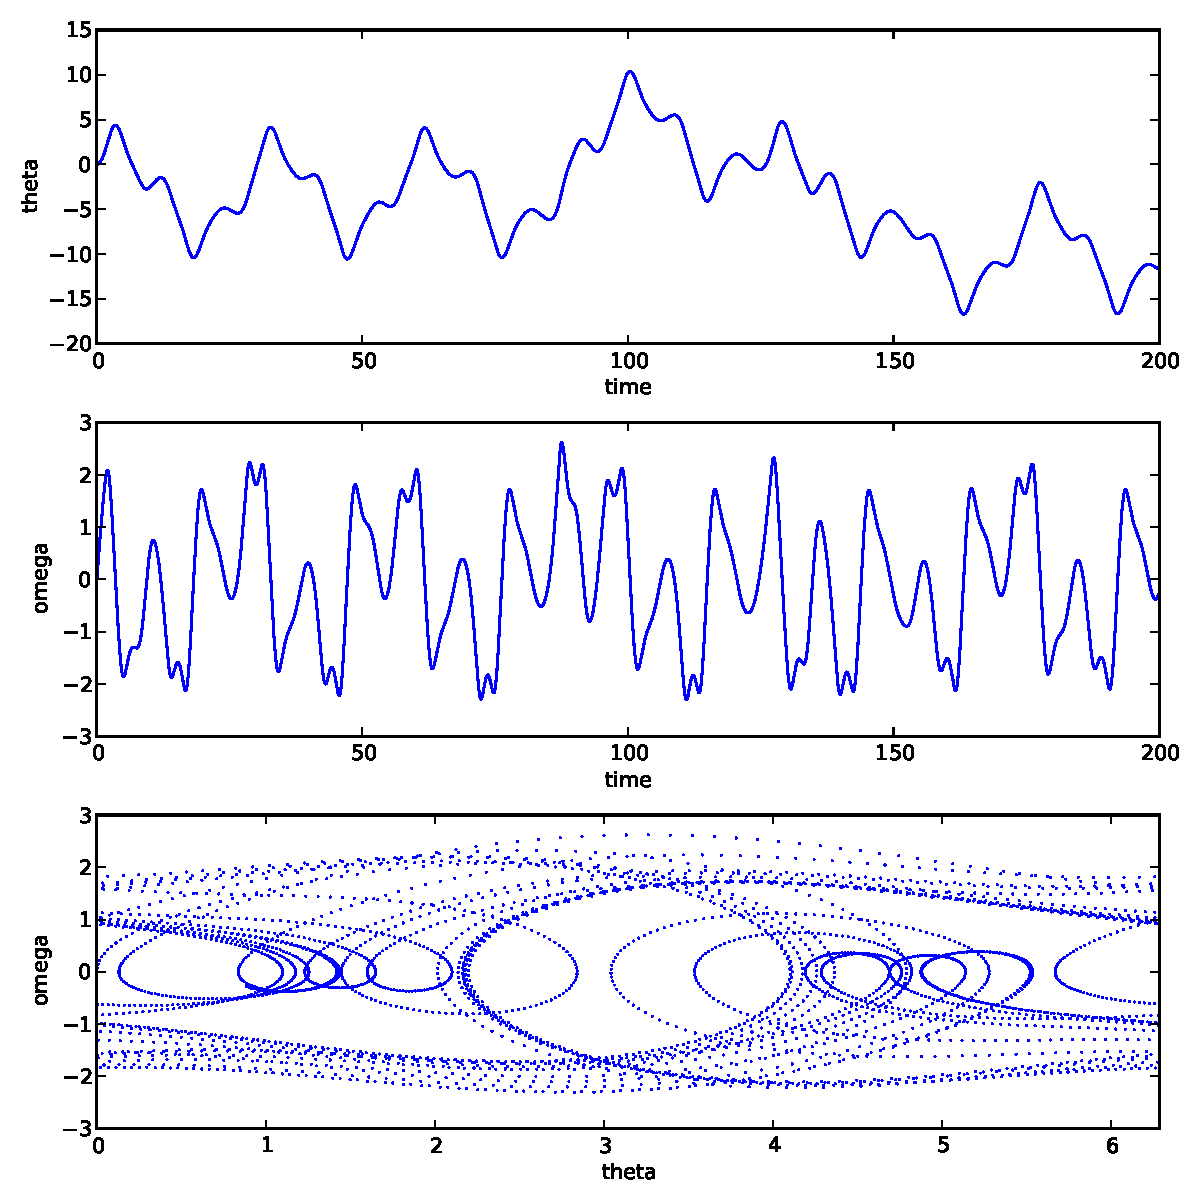
\includegraphics{odePend.pdf}}
\caption{Pendulum trajectory}\label{chap9/chap9_scipy:fig-odepend}\end{figure}

The plots above reveal that for the particular set of input parameters chosen, \code{Q = 2.0}, \code{d = 1.5}, and \code{Omega = 0.65}, the pendulum trajectories are chaotic.  Weaker forcing (smaller \(d\)) leads to what is perhaps the more familiar behavior of sinusoidal oscillations with a fixed frequency which, at long times, is equal to the driving frequency.

\index{discrete Fourier transforms}\index{fast Fourier transforms|see{discrete Fourier transforms}}\index{FFTs|see{discrete Fourier transforms}}

\section{Discrete (fast) Fourier transforms}
\label{chap9/chap9_scipy:index-5}\label{chap9/chap9_scipy:discrete-fast-fourier-transforms}
The SciPy library has a number of routines for performing discrete Fourier transforms.  Before delving into them, we provide a brief review of Fourier transforms and discrete Fourier transforms.


\subsection{Continuous and discrete Fourier transforms}
\label{chap9/chap9_scipy:continuous-and-discrete-fourier-transforms}
The Fourier transform of a function \(g(t)\) is given by
\phantomsection\label{chap9/chap9_scipy:equation-eq:FT}\begin{gather}
\begin{split} G(f) = \int_{-\infty}^\infty g(t)\, e^{-i\, 2\pi f t}\, dt \;,\end{split}\label{chap9/chap9_scipy-eq:FT}
\end{gather}
where \(f\) is the Fourier transform variable; if \(t\) is time, then \(f\) is frequency.  The inverse transform is given by
\phantomsection\label{chap9/chap9_scipy:equation-eq:iFT}\begin{gather}
\begin{split} g(t) = \int_{-\infty}^\infty G(f)\, e^{i\, 2\pi ft}\, df\end{split}\label{chap9/chap9_scipy-eq:iFT}
\end{gather}
Here we define the Fourier transform in terms of the frequency \(f\) rather than the angular frequency \(\omega = 2\pi f\).

The conventional Fourier transform is defined for continuous functions, or at least for functions that are dense and thus have an infinite number of data points.  When doing numerical analysis, however, you work with \emph{discrete} data sets, that is, data sets defined for a finite number of points.  The discrete Fourier transform (DFT) is defined for a function \(g_n\) consisting of a set of \(N\) discrete data points.  Those \(N\) data points must be defined at \emph{equally-spaced} times \(t_n=n\Delta t\) where \(\Delta t\) is the time between successive data points and \(n\) runs from 0 to \(N-1\).  The discrete Fourier transform (DFT) of \(g_n\) is defined as
\phantomsection\label{chap9/chap9_scipy:equation-eq:DFT}\begin{gather}
\begin{split}G_l = \sum_{n=0}^{N-1} g_n\, e^{-i\,(2\pi/N)\,ln}\end{split}\label{chap9/chap9_scipy-eq:DFT}
\end{gather}
where \(l\) runs from 0 to \(N-1\).  The inverse discrete Fourier transform (iDFT) is defined as
\phantomsection\label{chap9/chap9_scipy:equation-eq:iDFT}\begin{gather}
\begin{split}g_n = \frac{1}{N} \sum_{l=0}^{N-1} G_l\, e^{i\,(2\pi/N)\,ln} \;.\end{split}\label{chap9/chap9_scipy-eq:iDFT}
\end{gather}
The DFT is usually implemented on computers using the well-known Fast Fourier Transform (FFT) algorithm, generally credited to Cooley and Tukey who developed it at AT\&T Bell Laboratories during the 1960s.  But their algorithm is essentially one of many independent rediscoveries of the basic algorithm dating back to Gauss who described it as early as 1805.


\subsection{The SciPy FFT library}
\label{chap9/chap9_scipy:the-scipy-fft-library}
The SciPy library \code{scipy.fftpack} has routines that implement a souped-up version of the FFT algorithm along with many ancillary routines that support working with DFTs.  The basic FFT routine in \code{scipy.fftpack} is appropriately named \code{fft}.  The program below illustrates its use, along with the plots that follow.

\begin{Verbatim}[commandchars=\\\{\}]
\PYG{k+kn}{import} \PYG{n+nn}{numpy} \PYG{k+kn}{as} \PYG{n+nn}{np}
\PYG{k+kn}{from} \PYG{n+nn}{scipy} \PYG{k+kn}{import} \PYG{n}{fftpack}
\PYG{k+kn}{import} \PYG{n+nn}{matplotlib.pyplot} \PYG{k+kn}{as} \PYG{n+nn}{plt}

\PYG{n}{width} \PYG{o}{=} \PYG{l+m+mf}{2.0}
\PYG{n}{freq} \PYG{o}{=} \PYG{l+m+mf}{0.5}

\PYG{n}{t} \PYG{o}{=} \PYG{n}{np}\PYG{o}{.}\PYG{n}{linspace}\PYG{p}{(}\PYG{o}{\PYGZhy{}}\PYG{l+m+mi}{10}\PYG{p}{,} \PYG{l+m+mi}{10}\PYG{p}{,} \PYG{l+m+mi}{101}\PYG{p}{)}   \PYG{c}{\PYGZsh{} linearly space time array}
\PYG{n}{g} \PYG{o}{=} \PYG{n}{np}\PYG{o}{.}\PYG{n}{exp}\PYG{p}{(}\PYG{o}{\PYGZhy{}}\PYG{n}{np}\PYG{o}{.}\PYG{n}{abs}\PYG{p}{(}\PYG{n}{t}\PYG{p}{)}\PYG{o}{/}\PYG{n}{width}\PYG{p}{)} \PYG{o}{*} \PYG{n}{np}\PYG{o}{.}\PYG{n}{sin}\PYG{p}{(}\PYG{l+m+mf}{2.0}\PYG{o}{*}\PYG{n}{np}\PYG{o}{.}\PYG{n}{pi}\PYG{o}{*}\PYG{n}{freq}\PYG{o}{*}\PYG{n}{t}\PYG{p}{)}

\PYG{n}{dt} \PYG{o}{=} \PYG{n}{t}\PYG{p}{[}\PYG{l+m+mi}{1}\PYG{p}{]}\PYG{o}{\PYGZhy{}}\PYG{n}{t}\PYG{p}{[}\PYG{l+m+mi}{0}\PYG{p}{]}       \PYG{c}{\PYGZsh{} increment between times in time array}

\PYG{n}{G} \PYG{o}{=} \PYG{n}{fftpack}\PYG{o}{.}\PYG{n}{fft}\PYG{p}{(}\PYG{n}{g}\PYG{p}{)}   \PYG{c}{\PYGZsh{} FFT of g}
\PYG{n}{f} \PYG{o}{=} \PYG{n}{fftpack}\PYG{o}{.}\PYG{n}{fftfreq}\PYG{p}{(}\PYG{n}{g}\PYG{o}{.}\PYG{n}{size}\PYG{p}{,} \PYG{n}{d}\PYG{o}{=}\PYG{n}{dt}\PYG{p}{)} \PYG{c}{\PYGZsh{} frequenies f[i] of g[i]}
\PYG{n}{f} \PYG{o}{=} \PYG{n}{fftpack}\PYG{o}{.}\PYG{n}{fftshift}\PYG{p}{(}\PYG{n}{f}\PYG{p}{)}     \PYG{c}{\PYGZsh{} shift frequencies from min to max}
\PYG{n}{G} \PYG{o}{=} \PYG{n}{fftpack}\PYG{o}{.}\PYG{n}{fftshift}\PYG{p}{(}\PYG{n}{G}\PYG{p}{)}     \PYG{c}{\PYGZsh{} shift G order to coorespond to f}

\PYG{n}{fig} \PYG{o}{=} \PYG{n}{plt}\PYG{o}{.}\PYG{n}{figure}\PYG{p}{(}\PYG{l+m+mi}{1}\PYG{p}{,} \PYG{n}{figsize}\PYG{o}{=}\PYG{p}{(}\PYG{l+m+mi}{8}\PYG{p}{,}\PYG{l+m+mi}{6}\PYG{p}{)}\PYG{p}{,} \PYG{n}{frameon}\PYG{o}{=}\PYG{n+nb+bp}{False}\PYG{p}{)}
\PYG{n}{ax1} \PYG{o}{=} \PYG{n}{fig}\PYG{o}{.}\PYG{n}{add\PYGZus{}subplot}\PYG{p}{(}\PYG{l+m+mi}{211}\PYG{p}{)}
\PYG{n}{ax1}\PYG{o}{.}\PYG{n}{plot}\PYG{p}{(}\PYG{n}{t}\PYG{p}{,} \PYG{n}{g}\PYG{p}{)}
\PYG{n}{ax1}\PYG{o}{.}\PYG{n}{set\PYGZus{}xlabel}\PYG{p}{(}\PYG{l+s}{\PYGZsq{}}\PYG{l+s}{t}\PYG{l+s}{\PYGZsq{}}\PYG{p}{)}
\PYG{n}{ax1}\PYG{o}{.}\PYG{n}{set\PYGZus{}ylabel}\PYG{p}{(}\PYG{l+s}{\PYGZsq{}}\PYG{l+s}{g(t)}\PYG{l+s}{\PYGZsq{}}\PYG{p}{)}

\PYG{n}{ax2} \PYG{o}{=} \PYG{n}{fig}\PYG{o}{.}\PYG{n}{add\PYGZus{}subplot}\PYG{p}{(}\PYG{l+m+mi}{212}\PYG{p}{)}
\PYG{n}{ax2}\PYG{o}{.}\PYG{n}{plot}\PYG{p}{(}\PYG{n}{f}\PYG{p}{,} \PYG{n}{np}\PYG{o}{.}\PYG{n}{real}\PYG{p}{(}\PYG{n}{G}\PYG{p}{)}\PYG{p}{,} \PYG{n}{color}\PYG{o}{=}\PYG{l+s}{\PYGZsq{}}\PYG{l+s}{dodgerblue}\PYG{l+s}{\PYGZsq{}}\PYG{p}{,} \PYG{n}{label}\PYG{o}{=}\PYG{l+s}{\PYGZsq{}}\PYG{l+s}{real part}\PYG{l+s}{\PYGZsq{}}\PYG{p}{)}
\PYG{n}{ax2}\PYG{o}{.}\PYG{n}{plot}\PYG{p}{(}\PYG{n}{f}\PYG{p}{,} \PYG{n}{np}\PYG{o}{.}\PYG{n}{imag}\PYG{p}{(}\PYG{n}{G}\PYG{p}{)}\PYG{p}{,} \PYG{n}{color}\PYG{o}{=}\PYG{l+s}{\PYGZsq{}}\PYG{l+s}{coral}\PYG{l+s}{\PYGZsq{}}\PYG{p}{,} \PYG{n}{label}\PYG{o}{=}\PYG{l+s}{\PYGZsq{}}\PYG{l+s}{imaginary part}\PYG{l+s}{\PYGZsq{}}\PYG{p}{)}
\PYG{n}{ax2}\PYG{o}{.}\PYG{n}{legend}\PYG{p}{(}\PYG{p}{)}
\PYG{n}{ax2}\PYG{o}{.}\PYG{n}{set\PYGZus{}xlabel}\PYG{p}{(}\PYG{l+s}{\PYGZsq{}}\PYG{l+s}{f}\PYG{l+s}{\PYGZsq{}}\PYG{p}{)}
\PYG{n}{ax2}\PYG{o}{.}\PYG{n}{set\PYGZus{}ylabel}\PYG{p}{(}\PYG{l+s}{\PYGZsq{}}\PYG{l+s}{G(f)}\PYG{l+s}{\PYGZsq{}}\PYG{p}{)}

\PYG{n}{plt}\PYG{o}{.}\PYG{n}{show}\PYG{p}{(}\PYG{p}{)}
\end{Verbatim}
\begin{figure}[htbp]
\centering
\capstart

\scalebox{0.800000}{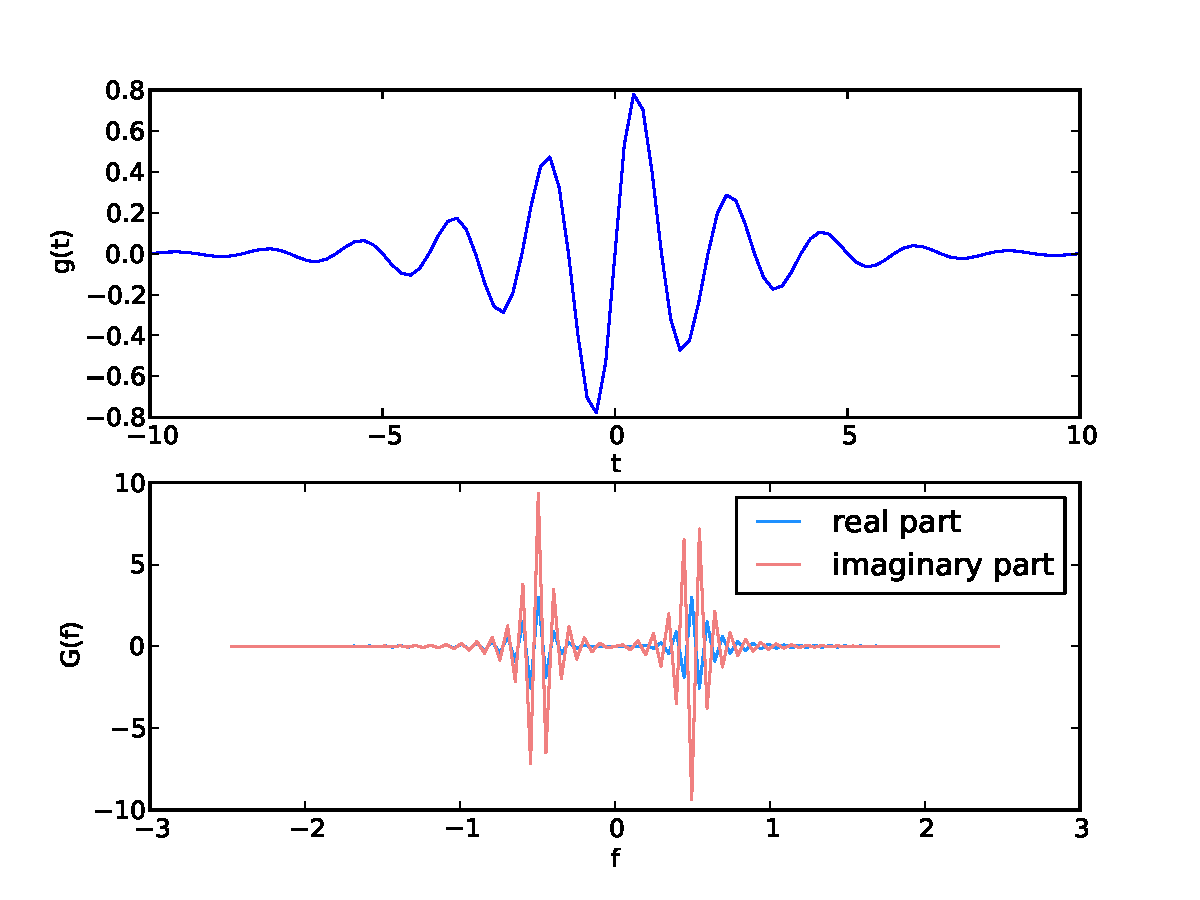
\includegraphics{fftSimple.pdf}}
\caption{Function \(g(t)\) and its DFT \(G(f)\).}\label{chap9/chap9_scipy:fig-fftsimple}\end{figure}

The DFT has real and imaginary parts, both of which are plotted in the figure.

The \code{fft} function returns the \(N\) Fourier components of \(G_n\) starting with the zero-frequency component \(G_0\) and progressing to the maximum positive frequency component \(G_{(N/2)-1}\) (or \(G_{(N-1)/2}\) if \(N\) is odd).  From there, \code{fft} returns the maximum \emph{negative} component \(G_{N/2}\)  (or \(G_{(N-1)/2}\) if \(N\) is odd) and continues upward in frequency until it reaches the minimum negative frequency component \(G_{N-1}\).  This is the standard way that DFTs are ordered by most numerical DFT packages.  The \code{scipy.fftpack} function \code{fftfreq} creates the array of frequencies in this non-intuitive order such that \code{f{[}n{]}} in the above routine is the correct frequency for the Fourier component \code{G{[}n{]}}.  The arguments of \code{fftfreq} are the size of the the orignal array \code{g} and the keyword argument \code{d} that is the spacing between the (equally spaced) elements of the time array (\code{d=1} if left unspecified).  The package \code{scipy.fftpack} provides the convenience function \code{fftshift} that reorders the frequency array so that the zero-frequency occurs at the middle of the array, that is, so the frequencies proceed monotonically from smallest (most negative) to largest (most positive).  Applying \code{fftshift} to both \code{f} and \code{G} puts the frequencies \code{f} in ascending order and shifts \code{G} so that the frequency of \code{G{[}n{]}} is given by the shifted \code{f{[}n{]}}.

The \code{scipy.fftpack} module also contains routines for performing 2-dimensional and \(n\)-dimensional DFTs, named \code{fft2} and \code{fftn}, respectively, using the FFT algorithm.

As for most FFT routines, the \code{scipy.fftpack} FFT routines are most efficient if \(N\) is a power of 2.  Nevertheless, the FFT routines are able to handle data sets where \(N\) is not a power of 2.

\code{scipy.fftpack} also supplies an inverse DFT function \code{ifft}.  It is written to act on the \emph{unshifted} FFT so take care!  Note also that \code{ifft} returns a \emph{complex} array.  Because of machine roundoff error, the imaginary part of the function returned by \code{ifft} will, in general, be very near zero but not exactly zero even when the original function is a purely real function.

\index{linear algebra}

\section{Linear algebra}
\label{chap9/chap9_scipy:index-6}\label{chap9/chap9_scipy:linear-algebra}
Python's mathematical libraries, NumPy and SciPy, have extensive tools for numerically solving problems in linear algebra.  Here we focus on two problems that arise commonly in scientific and engineering settings: (1) solving a system of linear equations and (2) eigenvalue problems.  In addition, we also show how to perform a number of other basic computations, such as finding the determinant of a matrix, matrix inversion, and \(LU\) decomposition.  The SciPy package for linear algebra is called \code{scipy.linalg}.


\subsection{Basic computations in linear algebra}
\label{chap9/chap9_scipy:basic-computations-in-linear-algebra}
SciPy has a number of routines for performing basic operations with matrices.  The determinant of a matrix is computed using the \code{scipy.linalg.det} function:

\begin{Verbatim}[commandchars=\\\{\}]
\PYG{g+gp}{In [1]: }\PYG{k+kn}{import} \PYG{n+nn}{scipy.linalg}
\PYG{g+gp}{In [2]: }\PYG{n}{a} \PYG{o}{=} \PYG{n}{array}\PYG{p}{(}\PYG{p}{[}\PYG{p}{[}\PYG{o}{\PYGZhy{}}\PYG{l+m+mi}{2}\PYG{p}{,} \PYG{l+m+mi}{3}\PYG{p}{]}\PYG{p}{,} \PYG{p}{[}\PYG{l+m+mi}{4}\PYG{p}{,} \PYG{l+m+mi}{5}\PYG{p}{]}\PYG{p}{]}\PYG{p}{)}
\PYG{g+gp}{In [3]: }\PYG{n}{a}
\PYG{g+gr}{Out[4]: }\PYG{n}{array}\PYG{p}{(}\PYG{p}{[}\PYG{p}{[}\PYG{o}{\PYGZhy{}}\PYG{l+m+mi}{2}\PYG{p}{,}  \PYG{l+m+mi}{3}\PYG{p}{]}\PYG{p}{,}
\PYG{g+go}{               [ 4,  5]])}

\PYG{g+gp}{In [5]: }\PYG{n}{scipy}\PYG{o}{.}\PYG{n}{linalg}\PYG{o}{.}\PYG{n}{det}\PYG{p}{(}\PYG{n}{a}\PYG{p}{)}
\PYG{g+gr}{Out[5]: }\PYG{o}{\PYGZhy{}}\PYG{l+m+mf}{22.0}
\end{Verbatim}

The inverse of a matrix is computed using the \code{scipy.linalg.inv} function, while the product of two matrices  is calculated using the NumPy \code{dot} function:

\begin{Verbatim}[commandchars=\\\{\}]
\PYG{g+gp}{In [6]: }\PYG{n}{b} \PYG{o}{=} \PYG{n}{scipy}\PYG{o}{.}\PYG{n}{linalg}\PYG{o}{.}\PYG{n}{inv}\PYG{p}{(}\PYG{n}{a}\PYG{p}{)}

\PYG{g+gp}{In [6]: }\PYG{n}{b}
\PYG{g+gr}{Out[6]: }\PYG{n}{array}\PYG{p}{(}\PYG{p}{[}\PYG{p}{[}\PYG{o}{\PYGZhy{}}\PYG{l+m+mf}{0.22727273}\PYG{p}{,}  \PYG{l+m+mf}{0.13636364}\PYG{p}{]}\PYG{p}{,}
\PYG{g+go}{               [ 0.18181818,  0.09090909]])}

\PYG{g+gp}{In [7]: }\PYG{n}{dot}\PYG{p}{(}\PYG{n}{a}\PYG{p}{,}\PYG{n}{b}\PYG{p}{)}
\PYG{g+gr}{Out[7]: }\PYG{n}{array}\PYG{p}{(}\PYG{p}{[}\PYG{p}{[} \PYG{l+m+mf}{1.}\PYG{p}{,}  \PYG{l+m+mf}{0.}\PYG{p}{]}\PYG{p}{,}
\PYG{g+go}{               [ 0.,  1.]])}
\end{Verbatim}

\index{linear algebra!solving systems of equations}

\subsection{Solving systems of linear equations}
\label{chap9/chap9_scipy:solving-systems-of-linear-equations}\label{chap9/chap9_scipy:index-7}
Solving systems of equations is nearly as simple as constructing a coefficient matrix and a column vector.  Suppose you have the following system of linear equations to solve:
\begin{gather}
\begin{split}2x_1 + 4x_2 + 6x_3 &= 4\\
 x_1 - 3x_2 - 9x_3 &= -11\\
8x_1 + 5x_2 - 7x_3 &= 1\\\end{split}\notag
\end{gather}
The first task is to recast this set of equations as a matrix equation of the form \(\mathsf{A}\, \mathbf{x} = \mathbf{b}\).  In this  case, we have:
\begin{gather}
\begin{split}\mathsf{A} = \left(\begin{array}{ccc}2 &  4 &  6 \\
                                     1 & -3 & -9 \\
                                     8 &  5 & -7 \end{array}\right)
                                     \;,\quad
\mathbf{x} = \left(\begin{array}{c}x_1 \\x_2 \\x_3\end{array}\right)
                                     \;,\quad
\mathbf{b} = \left(\begin{array}{c}4 \\-11 \\1\end{array}\right) \;.\end{split}\notag
\end{gather}
Next we construct the array \(\mathsf{A}\) and vector \(\mathbf{b}\) as NumPy arrays:

\begin{Verbatim}[commandchars=\\\{\}]
\PYG{g+gp}{In [8]: }\PYG{n}{A} \PYG{o}{=} \PYG{n}{array}\PYG{p}{(}\PYG{p}{[}\PYG{p}{[}\PYG{l+m+mi}{2}\PYG{p}{,} \PYG{l+m+mi}{4}\PYG{p}{,} \PYG{l+m+mi}{6}\PYG{p}{]}\PYG{p}{,} \PYG{p}{[}\PYG{l+m+mi}{1}\PYG{p}{,} \PYG{o}{\PYGZhy{}}\PYG{l+m+mi}{3}\PYG{p}{,} \PYG{o}{\PYGZhy{}}\PYG{l+m+mi}{9}\PYG{p}{]}\PYG{p}{,} \PYG{p}{[}\PYG{l+m+mi}{8}\PYG{p}{,} \PYG{l+m+mi}{5}\PYG{p}{,} \PYG{o}{\PYGZhy{}}\PYG{l+m+mi}{7}\PYG{p}{]}\PYG{p}{]}\PYG{p}{)}
\PYG{g+gp}{In [9]: }\PYG{n}{b} \PYG{o}{=} \PYG{n}{array}\PYG{p}{(}\PYG{p}{[}\PYG{l+m+mi}{4}\PYG{p}{,} \PYG{o}{\PYGZhy{}}\PYG{l+m+mi}{11}\PYG{p}{,} \PYG{l+m+mi}{2}\PYG{p}{]}\PYG{p}{)}
\end{Verbatim}

Finally we use the SciPy function \code{scipy.linalg.solve} to find \(x_1\), \(x_2\), and \(x_3\).

\begin{Verbatim}[commandchars=\\\{\}]
\PYG{g+gp}{In [10]: }\PYG{n}{scipy}\PYG{o}{.}\PYG{n}{linalg}\PYG{o}{.}\PYG{n}{solve}\PYG{p}{(}\PYG{n}{A}\PYG{p}{,}\PYG{n}{b}\PYG{p}{)}
\PYG{g+gr}{Out[10]: }\PYG{n}{array}\PYG{p}{(}\PYG{p}{[} \PYG{o}{\PYGZhy{}}\PYG{l+m+mf}{8.91304348}\PYG{p}{,}  \PYG{l+m+mf}{10.2173913} \PYG{p}{,}  \PYG{o}{\PYGZhy{}}\PYG{l+m+mf}{3.17391304}\PYG{p}{]}\PYG{p}{)}
\end{Verbatim}

which gives the results: \(x_1=-8.91304348\), \(x_2= 10.2173913\), and \(x_3= -3.17391304\).  Of course, you can get the same answer by noting that \(\mathbf{x}=\mathsf{A}^{-1}\mathbf{b}\).  Following this approach, we can use the \emph{scipy.linalg.inv} introduced in the previous section:

\begin{Verbatim}[commandchars=\\\{\}]
\PYG{g+go}{Ainv = scipy.linalg.inv(A)}

\PYG{g+gp}{In [10]: }\PYG{n}{dot}\PYG{p}{(}\PYG{n}{Ainv}\PYG{p}{,} \PYG{n}{b}\PYG{p}{)}
\PYG{g+gr}{Out[10]: }\PYG{n}{array}\PYG{p}{(}\PYG{p}{[} \PYG{o}{\PYGZhy{}}\PYG{l+m+mf}{8.91304348}\PYG{p}{,}  \PYG{l+m+mf}{10.2173913} \PYG{p}{,}  \PYG{o}{\PYGZhy{}}\PYG{l+m+mf}{3.17391304}\PYG{p}{]}\PYG{p}{)}
\end{Verbatim}

which is the same answer we obtained using \code{scipy.linalg.solve}.  Using \code{scipy.linalg.solve} is numerically more stable and a faster than using \(\mathbf{x}=\mathsf{A}^{-1}\mathbf{b}\), so it is the preferred method for solving systems of equations.

You might wonder what happens if the system of equations are not all linearly independent.  For example if the matrix \(\mathsf{A}\) is given by
\begin{gather}
\begin{split}\mathsf{A} = \left(\begin{array}{ccc}2 &  4 &  6 \\
                                     1 & -3 & -9 \\
                                     1 &  2 &  3 \end{array}\right)\end{split}\notag
\end{gather}
where the third row is a multiple of the first row.  Let's try it out and see what happens.  First we change the bottom row of the matrix \(\mathsf{A}\) and then try to solve the system as we did before.

\begin{Verbatim}[commandchars=\\\{\}]
\PYG{g+gp}{In [11]: }\PYG{n}{A}\PYG{p}{[}\PYG{l+m+mi}{2}\PYG{p}{]} \PYG{o}{=} \PYG{n}{array}\PYG{p}{(}\PYG{p}{[}\PYG{l+m+mi}{1}\PYG{p}{,} \PYG{l+m+mi}{2}\PYG{p}{,} \PYG{l+m+mi}{3}\PYG{p}{]}\PYG{p}{)}

\PYG{g+gp}{In [12]: }\PYG{n}{A}
\PYG{g+gr}{Out[12]: }\PYG{n}{array}\PYG{p}{(}\PYG{p}{[}\PYG{p}{[} \PYG{l+m+mi}{2}\PYG{p}{,}  \PYG{l+m+mi}{4}\PYG{p}{,}  \PYG{l+m+mi}{6}\PYG{p}{]}\PYG{p}{,}
\PYG{g+go}{                [ 1, \PYGZhy{}3, \PYGZhy{}9],}
\PYG{g+go}{                [ 1,  2,  3]])}

\PYG{g+gp}{In [13]: }\PYG{n}{scipy}\PYG{o}{.}\PYG{n}{linalg}\PYG{o}{.}\PYG{n}{solve}\PYG{p}{(}\PYG{n}{A}\PYG{p}{,}\PYG{n}{b}\PYG{p}{)}
\PYG{g+go}{LinAlgError: Singular matrix}

\PYG{g+gp}{In [14]: }\PYG{n}{Ainv} \PYG{o}{=} \PYG{n}{scipy}\PYG{o}{.}\PYG{n}{linalg}\PYG{o}{.}\PYG{n}{inv}\PYG{p}{(}\PYG{n}{A}\PYG{p}{)}
\PYG{g+go}{LinAlgError: Singular matrix}
\end{Verbatim}

Whether we use \code{scipy.linalg.solve} or \code{scipy.linalg.inv}, SciPy raises an error because the matrix is singular.

\index{linear algebra!eigenvalue problems}

\subsection{Eigenvalue problems}
\label{chap9/chap9_scipy:eigenvalue-problems}\label{chap9/chap9_scipy:index-8}
One of the most common problems in science and engineering is the eigenvalue problem, which in matrix form is written as
\begin{gather}
\begin{split}\mathsf{A}\mathbf{x} = \lambda \mathbf{x}\end{split}\notag
\end{gather}
where \(\mathsf{A}\) is a square matrix, \(\mathbf{x}\) is a column vector, and \(\lambda\) is a scalar (number).   Given the matrix \(\mathsf{A}\), the problem is to find the set of eigenvectors \(\mathbf{x}\) and their corresponding eigenvalues \(\lambda\) that solve this equation.

We can solve eigenvalue equations like this using \code{scipy.linalg.eig}. the outputs of this function is an array whose entries are the eigenvalues and a matrix whose rows are the eigenvectors.  Let's return to the matrix we were using previously and find its eigenvalues and eigenvectors.

\begin{Verbatim}[commandchars=\\\{\}]
\PYG{g+go}{A = array([[2, 4, 6],[1, \PYGZhy{}3, \PYGZhy{}9],[8, 5, \PYGZhy{}7]])}

\PYG{g+gp}{In [15]: }\PYG{n}{A}
\PYG{g+gr}{Out[15]: }\PYG{n}{array}\PYG{p}{(}\PYG{p}{[}\PYG{p}{[} \PYG{l+m+mi}{2}\PYG{p}{,}  \PYG{l+m+mi}{4}\PYG{p}{,}  \PYG{l+m+mi}{6}\PYG{p}{]}\PYG{p}{,}
\PYG{g+go}{                [ 1, \PYGZhy{}3, \PYGZhy{}9],}
\PYG{g+go}{                [ 8,  5, \PYGZhy{}7]])}

\PYG{g+gp}{In [16]: }\PYG{n}{lam}\PYG{p}{,} \PYG{n}{evec} \PYG{o}{=} \PYG{n}{scipy}\PYG{o}{.}\PYG{n}{linalg}\PYG{o}{.}\PYG{n}{eig}\PYG{p}{(}\PYG{n}{A}\PYG{p}{)}

\PYG{g+gp}{In [17]: }\PYG{n}{lam}
\PYG{g+gr}{Out[17]: }\PYG{n}{array}\PYG{p}{(}\PYG{p}{[} \PYG{l+m+mf}{2.40995356}\PYG{o}{+}\PYG{l+m+mf}{0.j}\PYG{p}{,} \PYG{o}{\PYGZhy{}}\PYG{l+m+mf}{8.03416016}\PYG{o}{+}\PYG{l+m+mf}{0.j}\PYG{p}{,}
\PYG{g+go}{                \PYGZhy{}2.37579340+0.j])}

\PYG{g+gp}{In [18]: }\PYG{n}{evec}
\PYG{g+gr}{Out[18]: }\PYG{n}{array}\PYG{p}{(}\PYG{p}{[}\PYG{p}{[}\PYG{o}{\PYGZhy{}}\PYG{l+m+mf}{0.77167559}\PYG{p}{,} \PYG{o}{\PYGZhy{}}\PYG{l+m+mf}{0.52633654}\PYG{p}{,}  \PYG{l+m+mf}{0.57513303}\PYG{p}{]}\PYG{p}{,}
\PYG{g+go}{                [ 0.50360249,  0.76565448, \PYGZhy{}0.80920669],}
\PYG{g+go}{                [\PYGZhy{}0.38846018,  0.36978786,  0.12002724]])}
\end{Verbatim}

The first eigenvalue and its corresponding eigenvector are given by

\begin{Verbatim}[commandchars=\\\{\}]
\PYG{g+gp}{In [19]: }\PYG{n}{lam}\PYG{p}{[}\PYG{l+m+mi}{0}\PYG{p}{]}
\PYG{g+gr}{Out[19]: }\PYG{p}{(}\PYG{l+m+mf}{2.4099535647625494}\PYG{o}{+}\PYG{l+m+mi}{0j}\PYG{p}{)}

\PYG{g+gp}{In [20]: }\PYG{n}{evec}\PYG{p}{[}\PYG{p}{:}\PYG{p}{,}\PYG{l+m+mi}{0}\PYG{p}{]}
\PYG{g+gr}{Out[20]: }\PYG{n}{array}\PYG{p}{(}\PYG{p}{[}\PYG{o}{\PYGZhy{}}\PYG{l+m+mf}{0.77167559}\PYG{p}{,}  \PYG{l+m+mf}{0.50360249}\PYG{p}{,} \PYG{o}{\PYGZhy{}}\PYG{l+m+mf}{0.38846018}\PYG{p}{]}\PYG{p}{)}
\end{Verbatim}

We can check that they satisfy the \(\mathsf{A}\mathbf{x} = \lambda \mathbf{x}:\)

\begin{Verbatim}[commandchars=\\\{\}]
\PYG{g+gp}{In [21]: }\PYG{n}{dot}\PYG{p}{(}\PYG{n}{A}\PYG{p}{,}\PYG{n}{evec}\PYG{p}{[}\PYG{p}{:}\PYG{p}{,}\PYG{l+m+mi}{0}\PYG{p}{]}\PYG{p}{)}
\PYG{g+gr}{Out[21]: }\PYG{n}{array}\PYG{p}{(}\PYG{p}{[}\PYG{o}{\PYGZhy{}}\PYG{l+m+mf}{1.85970234}\PYG{p}{,}  \PYG{l+m+mf}{1.21365861}\PYG{p}{,} \PYG{o}{\PYGZhy{}}\PYG{l+m+mf}{0.93617101}\PYG{p}{]}\PYG{p}{)}

\PYG{g+gp}{In [22]: }\PYG{n}{lam}\PYG{p}{[}\PYG{l+m+mi}{0}\PYG{p}{]}\PYG{o}{*}\PYG{n}{evec}\PYG{p}{[}\PYG{p}{:}\PYG{p}{,}\PYG{l+m+mi}{0}\PYG{p}{]}
\PYG{g+gr}{Out[22]: }\PYG{n}{array}\PYG{p}{(}\PYG{p}{[}\PYG{o}{\PYGZhy{}}\PYG{l+m+mf}{1.85970234}\PYG{o}{+}\PYG{l+m+mf}{0.j}\PYG{p}{,}  \PYG{l+m+mf}{1.21365861}\PYG{o}{+}\PYG{l+m+mf}{0.j}\PYG{p}{,}
\PYG{g+go}{                \PYGZhy{}0.93617101+0.j])}
\end{Verbatim}

Thus we see by direct substitution that the left and right sides of \(\mathsf{A}\mathbf{x} = \lambda \mathbf{x}:\) are equal.   In general, the eigenvalues can be complex, so their values are reported as complex numbers.

\index{linear algebra!generalized eigenvalue problem}

\subsubsection{Generalized eigenvalue problem}
\label{chap9/chap9_scipy:generalized-eigenvalue-problem}\label{chap9/chap9_scipy:index-9}
The \code{scipy.linalg.eig} function can also solve the \emph{generalized} eigenvalue problem
\begin{gather}
\begin{split}\mathsf{A}\mathbf{x} = \lambda \mathsf{B}\mathbf{x}\end{split}\notag
\end{gather}
where \(\mathsf{B}\) is a square matrix with the same size as \(\mathsf{A}\).  Suppose, for example, that we have

\begin{Verbatim}[commandchars=\\\{\}]
\PYG{g+gp}{In [22]: }\PYG{n}{A} \PYG{o}{=} \PYG{n}{array}\PYG{p}{(}\PYG{p}{[}\PYG{p}{[}\PYG{l+m+mi}{2}\PYG{p}{,} \PYG{l+m+mi}{4}\PYG{p}{,} \PYG{l+m+mi}{6}\PYG{p}{]}\PYG{p}{,} \PYG{p}{[}\PYG{l+m+mi}{1}\PYG{p}{,} \PYG{o}{\PYGZhy{}}\PYG{l+m+mi}{3}\PYG{p}{,} \PYG{o}{\PYGZhy{}}\PYG{l+m+mi}{9}\PYG{p}{]}\PYG{p}{,} \PYG{p}{[}\PYG{l+m+mi}{8}\PYG{p}{,} \PYG{l+m+mi}{5}\PYG{p}{,} \PYG{o}{\PYGZhy{}}\PYG{l+m+mi}{7}\PYG{p}{]}\PYG{p}{]}\PYG{p}{)}
\PYG{g+gr}{Out[22]: }\PYG{n}{B} \PYG{o}{=} \PYG{n}{array}\PYG{p}{(}\PYG{p}{[}\PYG{p}{[}\PYG{l+m+mi}{5}\PYG{p}{,} \PYG{l+m+mi}{9}\PYG{p}{,} \PYG{l+m+mi}{1}\PYG{p}{]}\PYG{p}{,} \PYG{p}{[}\PYG{o}{\PYGZhy{}}\PYG{l+m+mi}{3}\PYG{p}{,} \PYG{l+m+mi}{1}\PYG{p}{,} \PYG{l+m+mi}{6}\PYG{p}{]}\PYG{p}{,} \PYG{p}{[}\PYG{l+m+mi}{4}\PYG{p}{,} \PYG{l+m+mi}{2}\PYG{p}{,} \PYG{l+m+mi}{8}\PYG{p}{]}\PYG{p}{]}\PYG{p}{)}
\end{Verbatim}

Then we can solve the generalized eigenvalue problem by entering \(\mathsf{B}\) as the optional second argument to \code{scipy.linalg.eig}

\begin{Verbatim}[commandchars=\\\{\}]
\PYG{g+gp}{In [23]: }\PYG{n}{lam}\PYG{p}{,} \PYG{n}{evec} \PYG{o}{=} \PYG{n}{scipy}\PYG{o}{.}\PYG{n}{linalg}\PYG{o}{.}\PYG{n}{eig}\PYG{p}{(}\PYG{n}{A}\PYG{p}{,}\PYG{n}{B}\PYG{p}{)}
\end{Verbatim}

The solutions are returned in the same fashion as before, as an array \code{lam} whose entries are the eigenvalues and a matrix \code{evac} whose rows are the eigenvectors.

\begin{Verbatim}[commandchars=\\\{\}]
\PYG{g+gp}{In [24]: }\PYG{n}{lam}
\PYG{g+gr}{Out[24]: }\PYG{n}{array}\PYG{p}{(}\PYG{p}{[}\PYG{o}{\PYGZhy{}}\PYG{l+m+mf}{1.36087907}\PYG{o}{+}\PYG{l+m+mf}{0.j}\PYG{p}{,}  \PYG{l+m+mf}{0.83252442}\PYG{o}{+}\PYG{l+m+mf}{0.j}\PYG{p}{,}
\PYG{g+go}{                \PYGZhy{}0.10099858+0.j])}

\PYG{g+gp}{In [25]: }\PYG{n}{evec}
\PYG{g+gr}{Out[25]: }\PYG{n}{array}\PYG{p}{(}\PYG{p}{[}\PYG{p}{[}\PYG{o}{\PYGZhy{}}\PYG{l+m+mf}{0.0419907} \PYG{p}{,} \PYG{o}{\PYGZhy{}}\PYG{l+m+mf}{1.}        \PYG{p}{,}  \PYG{l+m+mf}{0.93037493}\PYG{p}{]}\PYG{p}{,}
\PYG{g+go}{                [\PYGZhy{}0.43028153,  0.17751302, \PYGZhy{}1.        ],}
\PYG{g+go}{                [ 1.        , \PYGZhy{}0.29852465,  0.4226201 ]])}
\end{Verbatim}

\index{linear algebra!Hermitian and banded matrices}

\subsubsection{Hermitian and banded matrices}
\label{chap9/chap9_scipy:hermitian-and-banded-matrices}\label{chap9/chap9_scipy:index-10}
SciPy has a specialized routine for solving eigenvalue problems for Hermitian (or real symmetric) matrices.  The routine for hermitian matrices is \code{scipy.linalg.eigh}.  It is more efficient (faster and uses less memory) than \code{scipy.linalg.eig}.  The basic syntax of the two routines is the same, although some of the \emph{optional} arguments are different.  Both routines can solve generalized as well as standard eigenvalue problems.

SciPy also has a specialized routine \code{scipy.linalg.eig\_banded} for solving eigenvalue problems for real symmetric or complex hermitian banded matrices.

\index{non-linear equations}\index{non-linear equations!solving}\index{solving non-linear equations|see{non-linear equations}}\index{roots of equations|see{non-linear equations}}

\section{Solving non-linear equations}
\label{chap9/chap9_scipy:solving-non-linear-equations}\label{chap9/chap9_scipy:sec-findingroots}\label{chap9/chap9_scipy:index-11}
SciPy has many different routines for numerically solving non-linear equations or systems of non-linear equations.  Here we will introduce only a few of these routines, the ones that are relatively simple and appropriate for the most common types of nonlinear equations.


\subsection{Single equations of a single variable}
\label{chap9/chap9_scipy:single-equations-of-a-single-variable}
Solving a single nonlinear equation is enormously simpler than solving a system of nonlinear equations, so that is where we start.  A word of caution: solving non-linear equations can be a tricky business so it is important that you have a good sense of the behavior of the function you are trying to solve.  The best way to do this is to plot the function over the domain of interest before trying to find the solutions.  This will greatly assist you in finding the solutions you seek and avoiding spurious solutions.

We begin with a concrete example.  Suppose we want to find the solutions to the equation
\begin{gather}
\begin{split}\tan x=\sqrt{(8/x)^2-1}\end{split}\notag
\end{gather}
Plots of \(\tan x\) and \(\sqrt{(8/x)^2-1}\) \emph{vs} \(x\) are shown in the top plot in the figure {\hyperref[chap5/chap5_plot:fig-subplotdemo]{\emph{Crossing functions}}}, albeit with \(x\) replaced by \(\theta\).  The solutions to this equation are those \(x\) values where the two curves \(\tan x\) and \(\sqrt{(8/x)^2-1}\) cross each other. The first step towards obtaining a numerical solution is to rewrite the equation to be solved in the form \(f(x)=0\).  Doing so, the above equation becomes
\begin{gather}
\begin{split}\tan x - \sqrt{(8/x)^2-1} = 0\end{split}\notag
\end{gather}
Obviously the two equations above have the same solutions for \(x\).  Parenthetically we mention that the problem of finding the solutions to equations of the form \(f(x)=0\) is often referred to as \emph{finding the roots} of \(f(x)\).

Next, we plot \(f(x)\) over the domain of interest, in this case from \(x=0\) to 8.  We are only interested in positive solutions and for \(x>8\), the equation has no real solutions as the argument of the square root becomes negative.  The solutions, the points where \(f(x)=0\) are indicated by green circles; there are three of them. Another notable feature of the function is that it diverges to \(\pm\infty\) at \(x = \{0, \pi/2, 3\pi/2, 5\pi/2\}\).
\begin{figure}[htbp]
\centering
\capstart

\scalebox{0.900000}{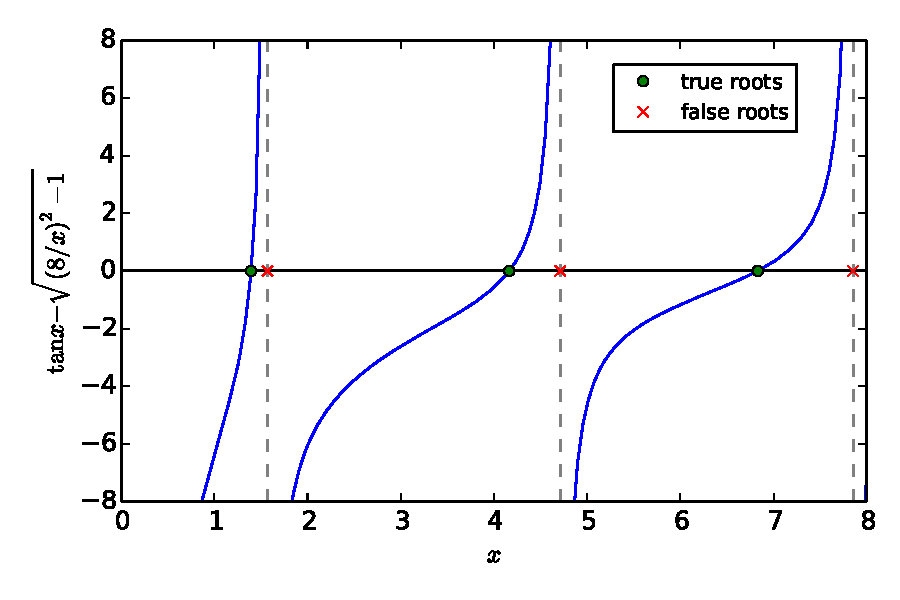
\includegraphics{rootsBrent.pdf}}
\caption{Roots of a nonlinear function}\label{chap9/chap9_scipy:fig-rootdemo}\end{figure}

\index{non-linear equations!Brent method}

\subsubsection{Brent method}
\label{chap9/chap9_scipy:brent-method}\label{chap9/chap9_scipy:index-12}
One of the workhorses for finding solutions to a single variable nonlinear equation is the method of Brent, discussed in many texts on numerical methods.  SciPy's implementation of the Brent algorithm is the function \code{scipy.optimize.brentq(f, a, b)}, which has three required arguments.  The first \code{f} is the name of the user-defined function to be solved.  The next two, \code{a} and \code{b} are the \(x\) values that bracket the solution you are looking for.  You should choose \code{a} and \code{b} so that there is only one solutions in the interval between \code{a} and \code{b}.  Brent's method also requires that \code{f(a)} and \code{f(b)} have opposite signs; an error message is returned if they do not.  Thus to find the three solutions to \(\tan x - \sqrt{(8/x)^2-1} = 0\), we need to run \code{scipy.optimize.brentq(f, a, b)} three times using three different values of \code{a} and \code{b} that bracket each of the three solutions.  The program below illustrates the how to use \code{scipy.optimize.brentq}

\begin{Verbatim}[commandchars=\\\{\}]
\PYG{k+kn}{import} \PYG{n+nn}{numpy} \PYG{k+kn}{as} \PYG{n+nn}{np}
\PYG{k+kn}{import} \PYG{n+nn}{scipy.optimize}
\PYG{k+kn}{import} \PYG{n+nn}{matplotlib.pyplot} \PYG{k+kn}{as} \PYG{n+nn}{plt}

\PYG{k}{def} \PYG{n+nf}{tdl}\PYG{p}{(}\PYG{n}{x}\PYG{p}{)}\PYG{p}{:}
    \PYG{n}{y} \PYG{o}{=} \PYG{l+m+mf}{8.}\PYG{o}{/}\PYG{n}{x}
    \PYG{k}{return} \PYG{n}{np}\PYG{o}{.}\PYG{n}{tan}\PYG{p}{(}\PYG{n}{x}\PYG{p}{)} \PYG{o}{\PYGZhy{}} \PYG{n}{np}\PYG{o}{.}\PYG{n}{sqrt}\PYG{p}{(}\PYG{n}{y}\PYG{o}{*}\PYG{n}{y}\PYG{o}{\PYGZhy{}}\PYG{l+m+mf}{1.0}\PYG{p}{)}

\PYG{c}{\PYGZsh{} Find true roots}

\PYG{n}{rx1} \PYG{o}{=} \PYG{n}{scipy}\PYG{o}{.}\PYG{n}{optimize}\PYG{o}{.}\PYG{n}{brentq}\PYG{p}{(}\PYG{n}{tdl}\PYG{p}{,} \PYG{l+m+mf}{0.5}\PYG{p}{,} \PYG{l+m+mf}{0.49}\PYG{o}{*}\PYG{n}{np}\PYG{o}{.}\PYG{n}{pi}\PYG{p}{)}
\PYG{n}{rx2} \PYG{o}{=} \PYG{n}{scipy}\PYG{o}{.}\PYG{n}{optimize}\PYG{o}{.}\PYG{n}{brentq}\PYG{p}{(}\PYG{n}{tdl}\PYG{p}{,} \PYG{l+m+mf}{0.51}\PYG{o}{*}\PYG{n}{np}\PYG{o}{.}\PYG{n}{pi}\PYG{p}{,} \PYG{l+m+mf}{1.49}\PYG{o}{*}\PYG{n}{np}\PYG{o}{.}\PYG{n}{pi}\PYG{p}{)}
\PYG{n}{rx3} \PYG{o}{=} \PYG{n}{scipy}\PYG{o}{.}\PYG{n}{optimize}\PYG{o}{.}\PYG{n}{brentq}\PYG{p}{(}\PYG{n}{tdl}\PYG{p}{,} \PYG{l+m+mf}{1.51}\PYG{o}{*}\PYG{n}{np}\PYG{o}{.}\PYG{n}{pi}\PYG{p}{,} \PYG{l+m+mf}{2.49}\PYG{o}{*}\PYG{n}{np}\PYG{o}{.}\PYG{n}{pi}\PYG{p}{)}
\PYG{n}{rx} \PYG{o}{=} \PYG{n}{np}\PYG{o}{.}\PYG{n}{array}\PYG{p}{(}\PYG{p}{[}\PYG{n}{rx1}\PYG{p}{,} \PYG{n}{rx2}\PYG{p}{,} \PYG{n}{rx3}\PYG{p}{]}\PYG{p}{)}
\PYG{n}{ry} \PYG{o}{=} \PYG{n}{np}\PYG{o}{.}\PYG{n}{zeros}\PYG{p}{(}\PYG{l+m+mi}{3}\PYG{p}{)}
\PYG{c}{\PYGZsh{} print using a list comprehension}
\PYG{k}{print}\PYG{p}{(}\PYG{l+s}{\PYGZsq{}}\PYG{l+s+se}{\PYGZbs{}n}\PYG{l+s}{True roots:}\PYG{l+s}{\PYGZsq{}}\PYG{p}{)}
\PYG{k}{print}\PYG{p}{(}\PYG{l+s}{\PYGZsq{}}\PYG{l+s+se}{\PYGZbs{}n}\PYG{l+s}{\PYGZsq{}}\PYG{o}{.}\PYG{n}{join}\PYG{p}{(}\PYG{l+s}{\PYGZsq{}}\PYG{l+s}{f(\PYGZob{}0:0.5f\PYGZcb{}) = \PYGZob{}1:0.2e\PYGZcb{}}\PYG{l+s}{\PYGZsq{}}\PYG{o}{.}\PYG{n}{format}\PYG{p}{(}\PYG{n}{x}\PYG{p}{,} \PYG{n}{tdl}\PYG{p}{(}\PYG{n}{x}\PYG{p}{)}\PYG{p}{)} \PYG{k}{for} \PYG{n}{x} \PYG{o+ow}{in} \PYG{n}{rx}\PYG{p}{)}\PYG{p}{)}

\PYG{c}{\PYGZsh{} Find false roots}

\PYG{n}{rx1f} \PYG{o}{=} \PYG{n}{scipy}\PYG{o}{.}\PYG{n}{optimize}\PYG{o}{.}\PYG{n}{brentq}\PYG{p}{(}\PYG{n}{tdl}\PYG{p}{,} \PYG{l+m+mf}{0.49}\PYG{o}{*}\PYG{n}{np}\PYG{o}{.}\PYG{n}{pi}\PYG{p}{,} \PYG{l+m+mf}{0.51}\PYG{o}{*}\PYG{n}{np}\PYG{o}{.}\PYG{n}{pi}\PYG{p}{)}
\PYG{n}{rx2f} \PYG{o}{=} \PYG{n}{scipy}\PYG{o}{.}\PYG{n}{optimize}\PYG{o}{.}\PYG{n}{brentq}\PYG{p}{(}\PYG{n}{tdl}\PYG{p}{,} \PYG{l+m+mf}{1.49}\PYG{o}{*}\PYG{n}{np}\PYG{o}{.}\PYG{n}{pi}\PYG{p}{,} \PYG{l+m+mf}{1.51}\PYG{o}{*}\PYG{n}{np}\PYG{o}{.}\PYG{n}{pi}\PYG{p}{)}
\PYG{n}{rx3f} \PYG{o}{=} \PYG{n}{scipy}\PYG{o}{.}\PYG{n}{optimize}\PYG{o}{.}\PYG{n}{brentq}\PYG{p}{(}\PYG{n}{tdl}\PYG{p}{,} \PYG{l+m+mf}{2.49}\PYG{o}{*}\PYG{n}{np}\PYG{o}{.}\PYG{n}{pi}\PYG{p}{,} \PYG{l+m+mf}{2.51}\PYG{o}{*}\PYG{n}{np}\PYG{o}{.}\PYG{n}{pi}\PYG{p}{)}
\PYG{n}{rxf} \PYG{o}{=} \PYG{n}{np}\PYG{o}{.}\PYG{n}{array}\PYG{p}{(}\PYG{p}{[}\PYG{n}{rx1f}\PYG{p}{,} \PYG{n}{rx2f}\PYG{p}{,} \PYG{n}{rx3f}\PYG{p}{]}\PYG{p}{)}
\PYG{c}{\PYGZsh{} print using a list comprehension}
\PYG{k}{print}\PYG{p}{(}\PYG{l+s}{\PYGZsq{}}\PYG{l+s+se}{\PYGZbs{}n}\PYG{l+s}{False roots:}\PYG{l+s}{\PYGZsq{}}\PYG{p}{)}
\PYG{k}{print}\PYG{p}{(}\PYG{l+s}{\PYGZsq{}}\PYG{l+s+se}{\PYGZbs{}n}\PYG{l+s}{\PYGZsq{}}\PYG{o}{.}\PYG{n}{join}\PYG{p}{(}\PYG{l+s}{\PYGZsq{}}\PYG{l+s}{f(\PYGZob{}0:0.5f\PYGZcb{}) = \PYGZob{}1:0.2e\PYGZcb{}}\PYG{l+s}{\PYGZsq{}}\PYG{o}{.}\PYG{n}{format}\PYG{p}{(}\PYG{n}{x}\PYG{p}{,} \PYG{n}{tdl}\PYG{p}{(}\PYG{n}{x}\PYG{p}{)}\PYG{p}{)} \PYG{k}{for} \PYG{n}{x} \PYG{o+ow}{in} \PYG{n}{rxf}\PYG{p}{)}\PYG{p}{)}

\PYG{c}{\PYGZsh{} Plot function and various roots}

\PYG{n}{x} \PYG{o}{=} \PYG{n}{np}\PYG{o}{.}\PYG{n}{linspace}\PYG{p}{(}\PYG{l+m+mf}{0.7}\PYG{p}{,} \PYG{l+m+mi}{8}\PYG{p}{,} \PYG{l+m+mi}{128}\PYG{p}{)}
\PYG{n}{y} \PYG{o}{=} \PYG{n}{tdl}\PYG{p}{(}\PYG{n}{x}\PYG{p}{)}
\PYG{c}{\PYGZsh{} Create masked array for plotting}
\PYG{n}{ymask} \PYG{o}{=} \PYG{n}{np}\PYG{o}{.}\PYG{n}{ma}\PYG{o}{.}\PYG{n}{masked\PYGZus{}where}\PYG{p}{(}\PYG{n}{np}\PYG{o}{.}\PYG{n}{abs}\PYG{p}{(}\PYG{n}{y}\PYG{p}{)}\PYG{o}{\PYGZgt{}}\PYG{l+m+mf}{20.}\PYG{p}{,} \PYG{n}{y}\PYG{p}{)}

\PYG{n}{plt}\PYG{o}{.}\PYG{n}{figure}\PYG{p}{(}\PYG{n}{figsize}\PYG{o}{=}\PYG{p}{(}\PYG{l+m+mi}{6}\PYG{p}{,} \PYG{l+m+mi}{4}\PYG{p}{)}\PYG{p}{)}
\PYG{n}{plt}\PYG{o}{.}\PYG{n}{plot}\PYG{p}{(}\PYG{n}{x}\PYG{p}{,} \PYG{n}{ymask}\PYG{p}{)}
\PYG{n}{plt}\PYG{o}{.}\PYG{n}{axhline}\PYG{p}{(}\PYG{n}{color}\PYG{o}{=}\PYG{l+s}{\PYGZsq{}}\PYG{l+s}{black}\PYG{l+s}{\PYGZsq{}}\PYG{p}{)}
\PYG{n}{plt}\PYG{o}{.}\PYG{n}{axvline}\PYG{p}{(}\PYG{n}{x}\PYG{o}{=}\PYG{n}{np}\PYG{o}{.}\PYG{n}{pi}\PYG{o}{/}\PYG{l+m+mf}{2.}\PYG{p}{,} \PYG{n}{color}\PYG{o}{=}\PYG{l+s}{\PYGZdq{}}\PYG{l+s}{gray}\PYG{l+s}{\PYGZdq{}}\PYG{p}{,} \PYG{n}{linestyle}\PYG{o}{=}\PYG{l+s}{\PYGZsq{}}\PYG{l+s}{\PYGZhy{}\PYGZhy{}}\PYG{l+s}{\PYGZsq{}}\PYG{p}{,} \PYG{n}{zorder}\PYG{o}{=}\PYG{o}{\PYGZhy{}}\PYG{l+m+mi}{1}\PYG{p}{)}
\PYG{n}{plt}\PYG{o}{.}\PYG{n}{axvline}\PYG{p}{(}\PYG{n}{x}\PYG{o}{=}\PYG{l+m+mf}{3.}\PYG{o}{*}\PYG{n}{np}\PYG{o}{.}\PYG{n}{pi}\PYG{o}{/}\PYG{l+m+mf}{2.}\PYG{p}{,} \PYG{n}{color}\PYG{o}{=}\PYG{l+s}{\PYGZdq{}}\PYG{l+s}{gray}\PYG{l+s}{\PYGZdq{}}\PYG{p}{,} \PYG{n}{linestyle}\PYG{o}{=}\PYG{l+s}{\PYGZsq{}}\PYG{l+s}{\PYGZhy{}\PYGZhy{}}\PYG{l+s}{\PYGZsq{}}\PYG{p}{,} \PYG{n}{zorder}\PYG{o}{=}\PYG{o}{\PYGZhy{}}\PYG{l+m+mi}{1}\PYG{p}{)}
\PYG{n}{plt}\PYG{o}{.}\PYG{n}{axvline}\PYG{p}{(}\PYG{n}{x}\PYG{o}{=}\PYG{l+m+mf}{5.}\PYG{o}{*}\PYG{n}{np}\PYG{o}{.}\PYG{n}{pi}\PYG{o}{/}\PYG{l+m+mf}{2.}\PYG{p}{,} \PYG{n}{color}\PYG{o}{=}\PYG{l+s}{\PYGZdq{}}\PYG{l+s}{gray}\PYG{l+s}{\PYGZdq{}}\PYG{p}{,} \PYG{n}{linestyle}\PYG{o}{=}\PYG{l+s}{\PYGZsq{}}\PYG{l+s}{\PYGZhy{}\PYGZhy{}}\PYG{l+s}{\PYGZsq{}}\PYG{p}{,} \PYG{n}{zorder}\PYG{o}{=}\PYG{o}{\PYGZhy{}}\PYG{l+m+mi}{1}\PYG{p}{)}
\PYG{n}{plt}\PYG{o}{.}\PYG{n}{xlabel}\PYG{p}{(}\PYG{l+s}{r\PYGZsq{}}\PYG{l+s}{\PYGZdl{}x\PYGZdl{}}\PYG{l+s}{\PYGZsq{}}\PYG{p}{)}
\PYG{n}{plt}\PYG{o}{.}\PYG{n}{ylabel}\PYG{p}{(}\PYG{l+s}{r\PYGZsq{}}\PYG{l+s}{\PYGZdl{}}\PYG{l+s}{\PYGZbs{}}\PYG{l+s}{tan x \PYGZhy{} }\PYG{l+s}{\PYGZbs{}}\PYG{l+s}{sqrt\PYGZob{}(8/x)\PYGZca{}2\PYGZhy{}1\PYGZcb{}\PYGZdl{}}\PYG{l+s}{\PYGZsq{}}\PYG{p}{)}
\PYG{n}{plt}\PYG{o}{.}\PYG{n}{ylim}\PYG{p}{(}\PYG{o}{\PYGZhy{}}\PYG{l+m+mi}{8}\PYG{p}{,} \PYG{l+m+mi}{8}\PYG{p}{)}

\PYG{n}{plt}\PYG{o}{.}\PYG{n}{plot}\PYG{p}{(}\PYG{n}{rx}\PYG{p}{,} \PYG{n}{ry}\PYG{p}{,} \PYG{l+s}{\PYGZsq{}}\PYG{l+s}{og}\PYG{l+s}{\PYGZsq{}}\PYG{p}{,} \PYG{n}{ms}\PYG{o}{=}\PYG{l+m+mi}{5}\PYG{p}{,} \PYG{n}{label}\PYG{o}{=}\PYG{l+s}{\PYGZsq{}}\PYG{l+s}{true roots}\PYG{l+s}{\PYGZsq{}}\PYG{p}{)}

\PYG{n}{plt}\PYG{o}{.}\PYG{n}{plot}\PYG{p}{(}\PYG{n}{rxf}\PYG{p}{,} \PYG{n}{ry}\PYG{p}{,} \PYG{l+s}{\PYGZsq{}}\PYG{l+s}{xr}\PYG{l+s}{\PYGZsq{}}\PYG{p}{,} \PYG{n}{ms}\PYG{o}{=}\PYG{l+m+mi}{5}\PYG{p}{,} \PYG{n}{label}\PYG{o}{=}\PYG{l+s}{\PYGZsq{}}\PYG{l+s}{false roots}\PYG{l+s}{\PYGZsq{}}\PYG{p}{)}
\PYG{n}{plt}\PYG{o}{.}\PYG{n}{legend}\PYG{p}{(}\PYG{n}{numpoints}\PYG{o}{=}\PYG{l+m+mi}{1}\PYG{p}{,} \PYG{n}{fontsize}\PYG{o}{=}\PYG{l+s}{\PYGZsq{}}\PYG{l+s}{small}\PYG{l+s}{\PYGZsq{}}\PYG{p}{,} \PYG{n}{loc} \PYG{o}{=} \PYG{l+s}{\PYGZsq{}}\PYG{l+s}{upper right}\PYG{l+s}{\PYGZsq{}}\PYG{p}{,}
           \PYG{n}{bbox\PYGZus{}to\PYGZus{}anchor} \PYG{o}{=} \PYG{p}{(}\PYG{l+m+mf}{0.92}\PYG{p}{,} \PYG{l+m+mf}{0.97}\PYG{p}{)}\PYG{p}{)}
\PYG{n}{plt}\PYG{o}{.}\PYG{n}{tight\PYGZus{}layout}\PYG{p}{(}\PYG{p}{)}
\PYG{n}{plt}\PYG{o}{.}\PYG{n}{show}\PYG{p}{(}\PYG{p}{)}
\end{Verbatim}

Running this code generates the following output:

\begin{Verbatim}[commandchars=\\\{\}]
\PYG{g+gp}{In [1]: }\PYG{n}{run} \PYG{n}{rootbrentq}\PYG{o}{.}\PYG{n}{py}

\PYG{g+go}{True roots:}
\PYG{g+go}{f(1.39547) = \PYGZhy{}6.39e\PYGZhy{}14}
\PYG{g+go}{f(4.16483) = \PYGZhy{}7.95e\PYGZhy{}14}
\PYG{g+go}{f(6.83067) = \PYGZhy{}1.11e\PYGZhy{}15}

\PYG{g+go}{False roots:}
\PYG{g+go}{f(1.57080) = \PYGZhy{}1.61e+12}
\PYG{g+go}{f(4.71239) = \PYGZhy{}1.56e+12}
\PYG{g+go}{f(7.85398) = 1.16e+12}
\end{Verbatim}

The Brent method finds the three true roots of the equation quickly and accurately when you provide values for the brackets \code{a} and \code{b} that are valid.  However, like many numerical methods for finding roots, the Brent method can produce spurious roots as it does in the above example when \code{a} and \code{b} bracket singularities like those at \(x = \{\pi/2, 3\pi/2, 5\pi/2\}\).  Here we evaluated the function at the purported roots found by \code{brentq} to verify that the values of \(x\) found were indeed roots.  For the true roots, the values of the function were very near zero, to within an acceptable roundoff error of less than \(10^{-13}\).  For the false roots, exceedingly large numbers on the order of  \(10^{12}\) were obtained, indicating a possible problem with these roots.  These results, together with the plots, allow you to unambiguously identify the true solutions to this nonlinear function.

The \code{brentq} function has a number of optional keyword arguments that you may find useful.  One keyword argument causes \code{brentq} to return not only the solution but the value of the function evaluated at the solution.  Other arguments allow you to specify a tolerance to which the solution is found as well as a few other parameters possibly of interest.  Most of the time, you can leave the keyword arguments at their default values.  See the \code{brentq} entry online on the SciPy web site for more information.

\index{non-linear equations!Newton-Raphson method}

\subsubsection{Other methods for solving equations of a single variable}
\label{chap9/chap9_scipy:index-13}\label{chap9/chap9_scipy:other-methods-for-solving-equations-of-a-single-variable}
SciPy provides a number of other methods for solving nonlinear equations of a single variable.  It has an implementation of the Newton-Raphson method called \code{scipy.optimize.newton}.  It's the racecar of such methods; its super fast but less stable that the Brent method.  To fully realize its speed, you need to specify not only the function to be solved, but also its first derivative, which is often more trouble than its worth.  You can also specify its second derivative, which may further speed up finding the solution.  If you do not specify the first or second derivatives, the method uses the secant method, which is usually slower than the Brent method.

\index{non-linear equations!Ridder method}\index{non-linear equations!Bisection method}
Other methods, including the Ridder (\code{scipy.optimize.ridder}) and bisection (\code{scipy.optimize.bisect}), are also available, although the Brent method is generally superior.  SciPy let's you use your favorite.

\index{non-linear equations!systems of nonlinear equations}

\subsection{Solving systems of nonlinear equations}
\label{chap9/chap9_scipy:solving-systems-of-nonlinear-equations}\label{chap9/chap9_scipy:index-15}
Solving systems of nonlinear equations is not for the faint of heart.  It is a difficult problem that lacks any general purpose solutions.  Nevertheless, SciPy provides quite an assortment of numerical solvers for nonlinear systems of equations.  However, because of the complexity and subtleties of this class of problems, we do not discuss their use here.
\newpage

\section{Exercises}
\label{chap9/chap9_scipy:exercises}\begin{enumerate}
\item {} 
Use NumPy's \code{polyval} function together with SciPy to plot the following functions:
\begin{enumerate}
\item {} 
The first four Chebyshev polynomials of first kind.  Plot these over the interval from -1 to +1.

\item {} 
The first four Hermite polynomials  \emph{multiplied} by \(e^{-x^2/2}\).  Plot these on the interval from -5 to +5.  These are the first four wave functions of the quantum mechanical simple harmonic oscillator.

\end{enumerate}

\end{enumerate}

\appendix
\phantomsection\label{apdx1/apdx1_install::doc}

\chapter{Installing Python}
\label{apdx1/apdx1_install:apdx1}\label{apdx1/apdx1_install:installing-python}
\index{Python!installing}
For scientific programming with Python, you need to install Python and three scientific Python libraries: NumPy, SciPy, and MatPlotLib.  There are many more libraries you can install, but Python along with NumPy, SciPy, and MatPlotLib are those that are essential for scientific programming.


\section{Installing Python}
\label{apdx1/apdx1_install:id1}
There are a number of ways to install Python and the scientific libraries you will need on your computer.  Some are easier than others.  You can install Python and the scientific libraries you need from ``source'' and compile them yourself.  This is not recommended unless you are an expert in Python, in which case you have little need for this manual.

\index{Canopy!installing Python}\index{installing Python!Canopy}\index{Spyder!installing Python}\index{installing Python!Spyder}
For most people, the simplest way to install Python and all the scientific libraries you need is to install either \emph{Canopy} or \emph{Spyder}.  Canopy and Spyder are integrated development environments (IDEs) for Python.  They have a number of very useful features and tools.  First, they have syntax highlighting, which colors different parts Python syntax according to function, making code easier to read.  Second, and more importantly, they run a program in the background called \emph{PyFlakes} that checks the validity of the Python syntax as you write it.  It's like a spelling and grammar checker all rolled into one, and it is extremely useful, for novice and expert alike.  The Canopy and Spyder IDEs have a number of other useful features, which we do not go into here, but expect you will learn about as you become more familiar with Python.  Canopy is a simpler IDE than Spyder, and easier for novices to learn and maintain.  Spyder has more advanced features, which you may find useful as you become more expert in Python programming.

\emph{Canopy} is written, maintained, and distributed by the software company Enthought (\href{http://www.enthought.com/}{http://www.enthought.com/}).  There are two versions of Canopy.  One version, \emph{Canopy Express}, is completely free to everybody and contains all the libraries you will need for this manual.  The other, \emph{Canopy Basic}, contains nearly every library you are ever likely to need for scientific computing.  It is free to academic users; others pay a fee.  Go to \href{https://www.enthought.com/products/canopy/}{https://www.enthought.com/products/canopy/} and press the ``Get Canopy'' button, which will take you to a page where you can either download \emph{Canopy Express} or request and academic license, which will allow you to download \emph{Canopy Basic}.

\emph{Spyder} provides a completely open source programming environment for Python.  The entire Spyder distribution is free to all and can be found at \href{https://code.google.com/p/spyderlib/}{https://code.google.com/p/spyderlib/}.  It also includes nearly all the scientific libraries you are likely to need for scientific computing.

In this manual, we assume you are using Canopy, but the Spyder interface is very similar to Canopy so that most users should have no difficulty using Spyder with this manual.  If you choose to use Spyder, launch Spyder and then go to the Preferences menu and then under the \code{Console} menu, select the \code{Advanced settings} tab; tick the box \code{Start an IPython kernel at startup} (it may already be selected, in which case you need to do nothing).  You only need to do this once, which sets up the IPython console when Spyder is launched.  Once that is done, you should be able to follow everything written in this manual.


\section{Testing your installation of Python}
\label{apdx1/apdx1_install:testing-your-installation-of-python}
Running the Python program below tests your installation of Python to verify that the installation was successful.  In particular, it tests that the NumPy, SciPy, and MatPlotLib libraries that are needed for this manual are properly installed.

If you are a student, you should input your first and last names inside the single quotes on lines 15 and 16, respectively.

Instructors can modify lines 21-23 to suit the needs of the course.

\begin{Verbatim}[commandchars=\\\{\},numbers=left,firstnumber=1,stepnumber=1]
\PYG{c}{\PYGZsh{} This code tests that your Python installation worked.}
\PYG{c}{\PYGZsh{} It generates a png image file that you should e\PYGZhy{}mail}
\PYG{c}{\PYGZsh{} to the address shown on the plot}
\PYG{k+kn}{import} \PYG{n+nn}{scipy}
\PYG{k+kn}{import} \PYG{n+nn}{numpy}
\PYG{k+kn}{import} \PYG{n+nn}{matplotlib}
\PYG{k+kn}{import} \PYG{n+nn}{matplotlib.pyplot} \PYG{k+kn}{as} \PYG{n+nn}{plt}
\PYG{k+kn}{import} \PYG{n+nn}{platform}
\PYG{k+kn}{import} \PYG{n+nn}{socket}

\PYG{c}{\PYGZsh{} If you are a student, please fill in your first and last}
\PYG{c}{\PYGZsh{} names inside the quotes in the two lines below.  Do not}
\PYG{c}{\PYGZsh{} modify anything else in this file}

\PYG{n}{your\PYGZus{}first\PYGZus{}name} \PYG{o}{=} \PYG{l+s}{\PYGZsq{}}\PYG{l+s}{Dana}\PYG{l+s}{\PYGZsq{}}
\PYG{n}{your\PYGZus{}last\PYGZus{}name} \PYG{o}{=} \PYG{l+s}{\PYGZsq{}}\PYG{l+s}{Martin}\PYG{l+s}{\PYGZsq{}}

\PYG{c}{\PYGZsh{} If you are an instructor, modify the next 3 lines.}
\PYG{c}{\PYGZsh{} You do not need to modify anything else in this file.}

\PYG{n}{classname} \PYG{o}{=} \PYG{l+s}{\PYGZsq{}}\PYG{l+s}{Intro Phys I}\PYG{l+s}{\PYGZsq{}}
\PYG{n}{term} \PYG{o}{=} \PYG{l+s}{\PYGZsq{}}\PYG{l+s}{Fall\PYGZus{}2014}\PYG{l+s}{\PYGZsq{}}      \PYG{c}{\PYGZsh{} must contain no spaces}
\PYG{n}{email} \PYG{o}{=} \PYG{l+s}{\PYGZsq{}}\PYG{l+s}{hmwkemail@univX.edu}\PYG{l+s}{\PYGZsq{}}

\PYG{n}{plt}\PYG{o}{.}\PYG{n}{plot}\PYG{p}{(}\PYG{p}{[}\PYG{l+m+mi}{0}\PYG{p}{,}\PYG{l+m+mi}{1}\PYG{p}{]}\PYG{p}{,} \PYG{l+s}{\PYGZsq{}}\PYG{l+s}{r}\PYG{l+s}{\PYGZsq{}}\PYG{p}{,} \PYG{p}{[}\PYG{l+m+mi}{1}\PYG{p}{,}\PYG{l+m+mi}{0}\PYG{p}{]}\PYG{p}{,} \PYG{l+s}{\PYGZsq{}}\PYG{l+s}{b}\PYG{l+s}{\PYGZsq{}}\PYG{p}{)}
\PYG{n}{plt}\PYG{o}{.}\PYG{n}{text}\PYG{p}{(} \PYG{l+m+mf}{0.5}\PYG{p}{,} \PYG{l+m+mf}{0.8}\PYG{p}{,} \PYG{l+s}{\PYGZsq{}}\PYG{l+s}{\PYGZob{}0:s\PYGZcb{} \PYGZob{}1:s\PYGZcb{}}\PYG{l+s}{\PYGZsq{}}
        \PYG{o}{.}\PYG{n}{format}\PYG{p}{(}\PYG{n}{your\PYGZus{}first\PYGZus{}name}\PYG{p}{,} \PYG{n}{your\PYGZus{}last\PYGZus{}name}\PYG{p}{)}\PYG{p}{,}
        \PYG{n}{horizontalalignment}\PYG{o}{=}\PYG{l+s}{\PYGZsq{}}\PYG{l+s}{center}\PYG{l+s}{\PYGZsq{}}\PYG{p}{,}
        \PYG{n}{size} \PYG{o}{=} \PYG{l+s}{\PYGZsq{}}\PYG{l+s}{x\PYGZhy{}large}\PYG{l+s}{\PYGZsq{}}\PYG{p}{,}
        \PYG{n}{bbox}\PYG{o}{=}\PYG{n+nb}{dict}\PYG{p}{(}\PYG{n}{facecolor}\PYG{o}{=}\PYG{l+s}{\PYGZsq{}}\PYG{l+s}{purple}\PYG{l+s}{\PYGZsq{}}\PYG{p}{,} \PYG{n}{alpha}\PYG{o}{=}\PYG{l+m+mf}{0.4}\PYG{p}{)}\PYG{p}{)}
\PYG{n}{plt}\PYG{o}{.}\PYG{n}{text}\PYG{p}{(} \PYG{l+m+mf}{0.5}\PYG{p}{,} \PYG{l+m+mf}{0.1}\PYG{p}{,}
    \PYG{l+s}{\PYGZsq{}}\PYG{l+s}{\PYGZob{}1:s\PYGZcb{}}\PYG{l+s+se}{\PYGZbs{}n}\PYG{l+s}{scipy \PYGZob{}2:s\PYGZcb{}}\PYG{l+s+se}{\PYGZbs{}n}\PYG{l+s}{numpy \PYGZob{}3:s\PYGZcb{}}\PYG{l+s+se}{\PYGZbs{}n}\PYG{l+s}{matplotlib \PYGZob{}4:s\PYGZcb{}}\PYG{l+s+se}{\PYGZbs{}n}\PYG{l+s}{on \PYGZob{}5:s\PYGZcb{}}\PYG{l+s+se}{\PYGZbs{}n}\PYG{l+s}{\PYGZob{}6:s\PYGZcb{}}\PYG{l+s}{\PYGZsq{}}
        \PYG{o}{.}\PYG{n}{format}\PYG{p}{(}
        \PYG{n}{classname}\PYG{p}{,}
        \PYG{n}{term}\PYG{p}{,}
        \PYG{n}{scipy}\PYG{o}{.}\PYG{n}{\PYGZus{}\PYGZus{}version\PYGZus{}\PYGZus{}}\PYG{p}{,}
        \PYG{n}{numpy}\PYG{o}{.}\PYG{n}{\PYGZus{}\PYGZus{}version\PYGZus{}\PYGZus{}}\PYG{p}{,}
        \PYG{n}{matplotlib}\PYG{o}{.}\PYG{n}{\PYGZus{}\PYGZus{}version\PYGZus{}\PYGZus{}}\PYG{p}{,}
        \PYG{n}{platform}\PYG{o}{.}\PYG{n}{platform}\PYG{p}{(}\PYG{p}{)}\PYG{p}{,}
        \PYG{n}{socket}\PYG{o}{.}\PYG{n}{gethostname}\PYG{p}{(}\PYG{p}{)}
        \PYG{p}{)} \PYG{p}{,}
    \PYG{n}{horizontalalignment}\PYG{o}{=}\PYG{l+s}{\PYGZsq{}}\PYG{l+s}{center}\PYG{l+s}{\PYGZsq{}}
    \PYG{p}{)}
\PYG{n}{filename} \PYG{o}{=} \PYG{n}{your\PYGZus{}last\PYGZus{}name} \PYG{o}{+} \PYG{l+s}{\PYGZsq{}}\PYG{l+s}{\PYGZus{}}\PYG{l+s}{\PYGZsq{}} \PYG{o}{+} \PYG{n}{your\PYGZus{}first\PYGZus{}name} \PYG{o}{+} \PYG{l+s}{\PYGZsq{}}\PYG{l+s}{\PYGZus{}}\PYG{l+s}{\PYGZsq{}} \PYG{o}{+} \PYG{n}{term} \PYG{o}{+} \PYG{l+s}{\PYGZsq{}}\PYG{l+s}{.png}\PYG{l+s}{\PYGZsq{}}
\PYG{n}{plt}\PYG{o}{.}\PYG{n}{title}\PYG{p}{(}\PYG{l+s}{\PYGZsq{}}\PYG{l+s}{*** E\PYGZhy{}mail the saved version of this plot, ***}\PYG{l+s+se}{\PYGZbs{}n}\PYG{l+s}{\PYGZsq{}} \PYG{o}{+}
    \PYG{l+s}{\PYGZsq{}}\PYG{l+s}{\PYGZdq{}}\PYG{l+s}{\PYGZob{}0:s\PYGZcb{}}\PYG{l+s}{\PYGZdq{}}\PYG{l+s}{ to \PYGZob{}1:s\PYGZcb{}}\PYG{l+s}{\PYGZsq{}}\PYG{o}{.}\PYG{n}{format}\PYG{p}{(}\PYG{n}{filename}\PYG{p}{,} \PYG{n}{email}\PYG{p}{)}\PYG{p}{,} \PYG{n}{fontsize}\PYG{o}{=}\PYG{l+m+mi}{12}\PYG{p}{)}
\PYG{n}{plt}\PYG{o}{.}\PYG{n}{savefig}\PYG{p}{(}\PYG{n}{filename}\PYG{p}{)}
\PYG{n}{plt}\PYG{o}{.}\PYG{n}{show}\PYG{p}{(}\PYG{p}{)}
\end{Verbatim}
\phantomsection\label{apdx2/apdx2_ipynb::doc}\phantomsection\label{apdx2/apdx2_ipynb:apdx2}
\index{IPython!IPython Notebook}

\chapter{IPython Notebooks}
\label{apdx2/apdx2_ipynb:ipython-notebooks}\label{apdx2/apdx2_ipynb:index-0}
IPython notebooks are useful for logging your work.  Here we suggest that you use them for logging and turning in homework assignments.  You may also find them useful in other contexts such as laboratory work.  The IPython Notebook interface is similar to Mathematica or Maple.


\section{An interactive interface}
\label{apdx2/apdx2_ipynb:an-interactive-interface}
An IPython notebook is a web-based environment for interactive computing.  You can work in this environment interactively just as you would using the IPython shell (the interactive Python pane shown in the {\hyperref[chap2/chap2_basics:fig-canopywindow]{\emph{Canopy window}}} figure).  In addition, you can also store and run programs in an IPython notebook just like you would from the Code Editor window (see {\hyperref[chap2/chap2_basics:fig-canopywindow]{\emph{Canopy window}}}).  Thus, it would seem that an IPython notebook and the Canopy environments do essentially the same thing.  Up to a point, that is true.  In the final analysis, however, Canopy (or Spyder or some similar Python development environment) is generally more useful for developing, storing, and running code.  An IPython Notebook, on the other hand, is excellent for logging your work in Python.  That is why we suggest using them for homework assignments.  You may find them useful in other contexts as well.


\section{Installing and launching an IPython notebook}
\label{apdx2/apdx2_ipynb:installing-and-launching-an-ipython-notebook}
If you have installed Canopy or Spyder, then you have already installed all the software you need to use IPython notebooks.  IPython notbooks are stored in files with a \code{.ipynb} extension.  To create an IPython notebook, launch the Terminal (Mac) or the Command Prompt (PC) application.  On the Mac, the Terminal application is found in the Applications/Utilies folder.  On the PC, the Command Prompt application is found under the Start/All Programs/Accessories menu.  Here we will refer the the Terminal or Command Prompt applications at the System Console.  Type \code{pwd} (Mac) or \code{chdir} (PC) to determine the current directory (folder) of the System Console.  Type \code{ls} (Mac) or \code{dir} (PC) to list all the files and subdirectories in the current directory.  Using the \code{cd} change directory command, move the System Console to the directory in which you want to store your IPython notebook.

At the System Console prompt, type
\begin{quote}

\begin{Verbatim}[commandchars=\\\{\}]
ipython notebook \PYGZhy{}\PYGZhy{}matplotlib inline \PYGZam{}
\end{Verbatim}
\end{quote}

This will launch the IPython notebook web application and will display the {\hyperref[apdx2/apdx2_ipynb:fig-nbdashboard]{\emph{IPython Notebook Home Page}}} as a page in your default web browser.
\begin{figure}[htbp]
\centering
\capstart

\scalebox{0.900000}{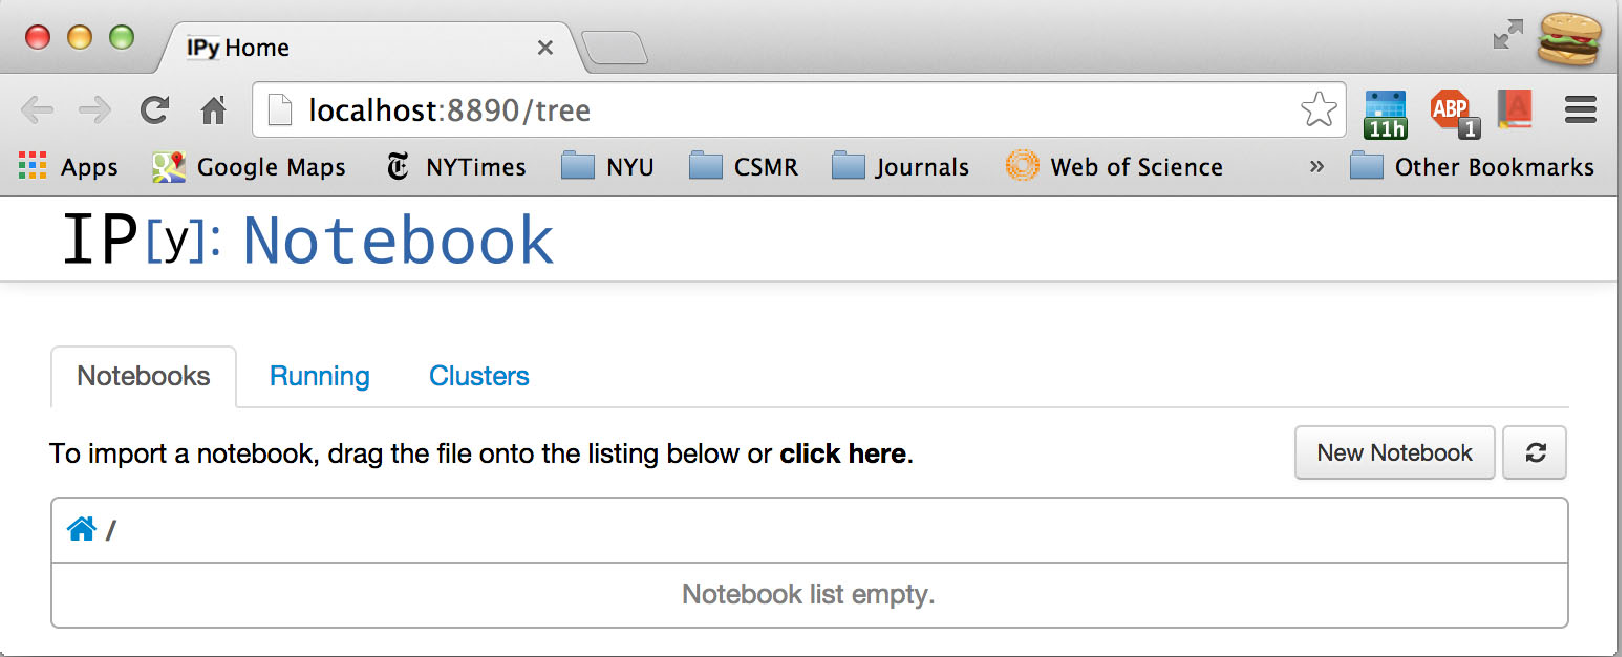
\includegraphics{nbDashboard.pdf}}
\caption{IPython Notebook Home Page}\label{apdx2/apdx2_ipynb:fig-nbdashboard}\end{figure}

To create a new IPython notebook, click the \code{New Notebook} button.  That will open a new {\hyperref[apdx2/apdx2_ipynb:fig-ipynotebook]{\emph{IPython Notebook}}} with the provisional title \code{Untitled0} in a new tab in your browser.  To give the notebook a more meaningful name, click on \code{Untitled0} in your browser window to the right of \code{IP{[}y{]}: Notebook} and  rename your notebook \code{FirstNotebook}.  The Name \code{FirstNotebook} will replace \code{Untitled0} in your Notebook browser window and a file named \code{FirstNotebook.ipynb} will appear in the directory from which you launched IPython Notebook.  That file will contain all the work you do in the IPython notebook.  Next time you launch IPython Notebook from this same directory, all the IPython notebooks in that directory will appear in a list on the IPython Notebook Dashboard.  Clicking on one of them will launch that notebook.
\begin{figure}[htbp]
\centering
\capstart

\scalebox{0.900000}{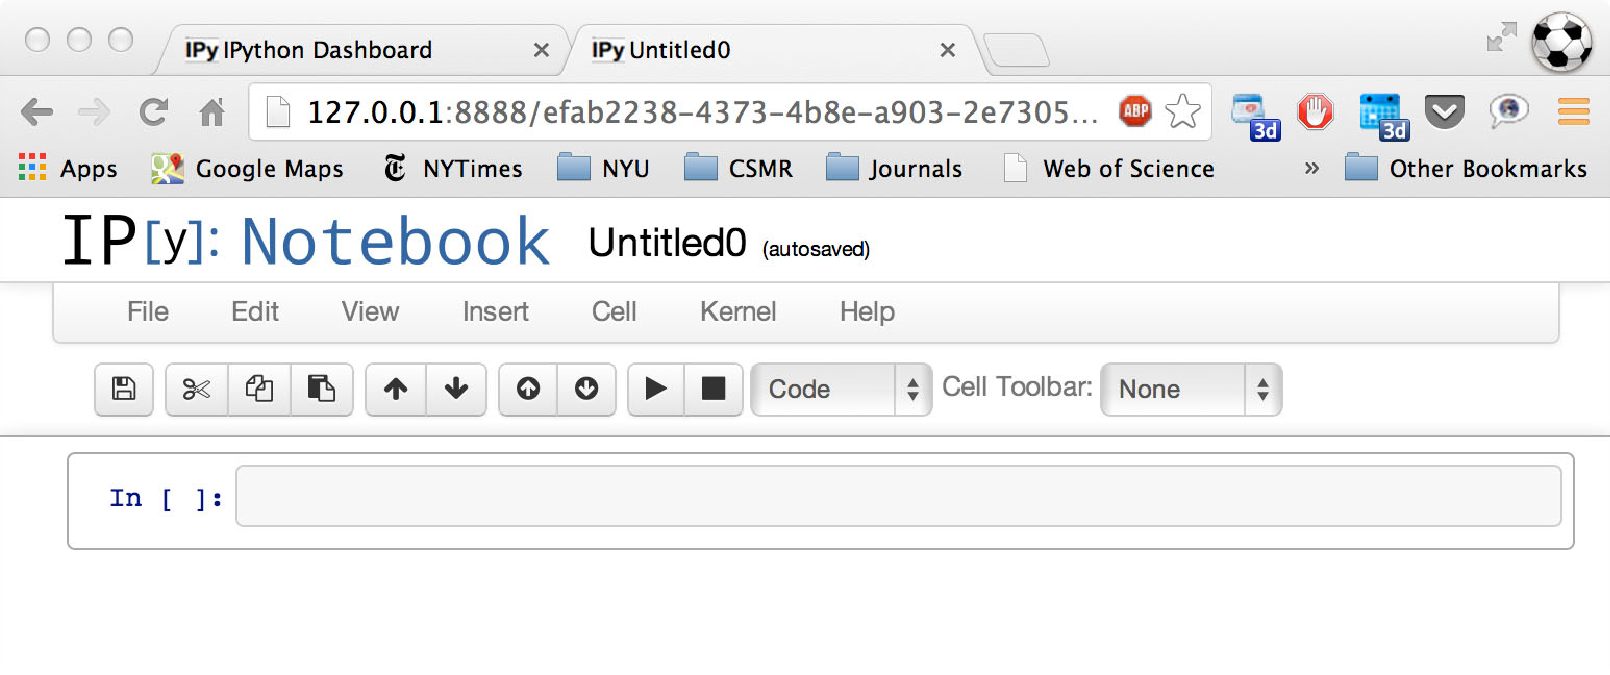
\includegraphics{ipyNotebook.pdf}}
\caption{IPython Notebook}\label{apdx2/apdx2_ipynb:fig-ipynotebook}\end{figure}


\section{Using an IPython Notebook}
\label{apdx2/apdx2_ipynb:using-an-ipython-notebook}
When you open a new IPython Notebook, an IPython interactive cell with the prompt \code{In{[} {]}:} to the left, appears.  You can type code into this cell just as you would in the IPython shell of the {\hyperref[chap2/chap2_basics:fig-canopywindow]{\emph{Canopy window}}}.  For example, typing \code{2+3} into the cell and pressing \code{Shift-Enter} (or \code{Shift-Return}) to execute the cell yields the expected result.  Try it out.  Typing \code{sin(pi/6.)} and pressing \code{Shift-Enter} produces the expected result (to nearly 1 part in \(10^{16}\)).
\begin{figure}[htbp]
\centering
\capstart

\scalebox{0.900000}{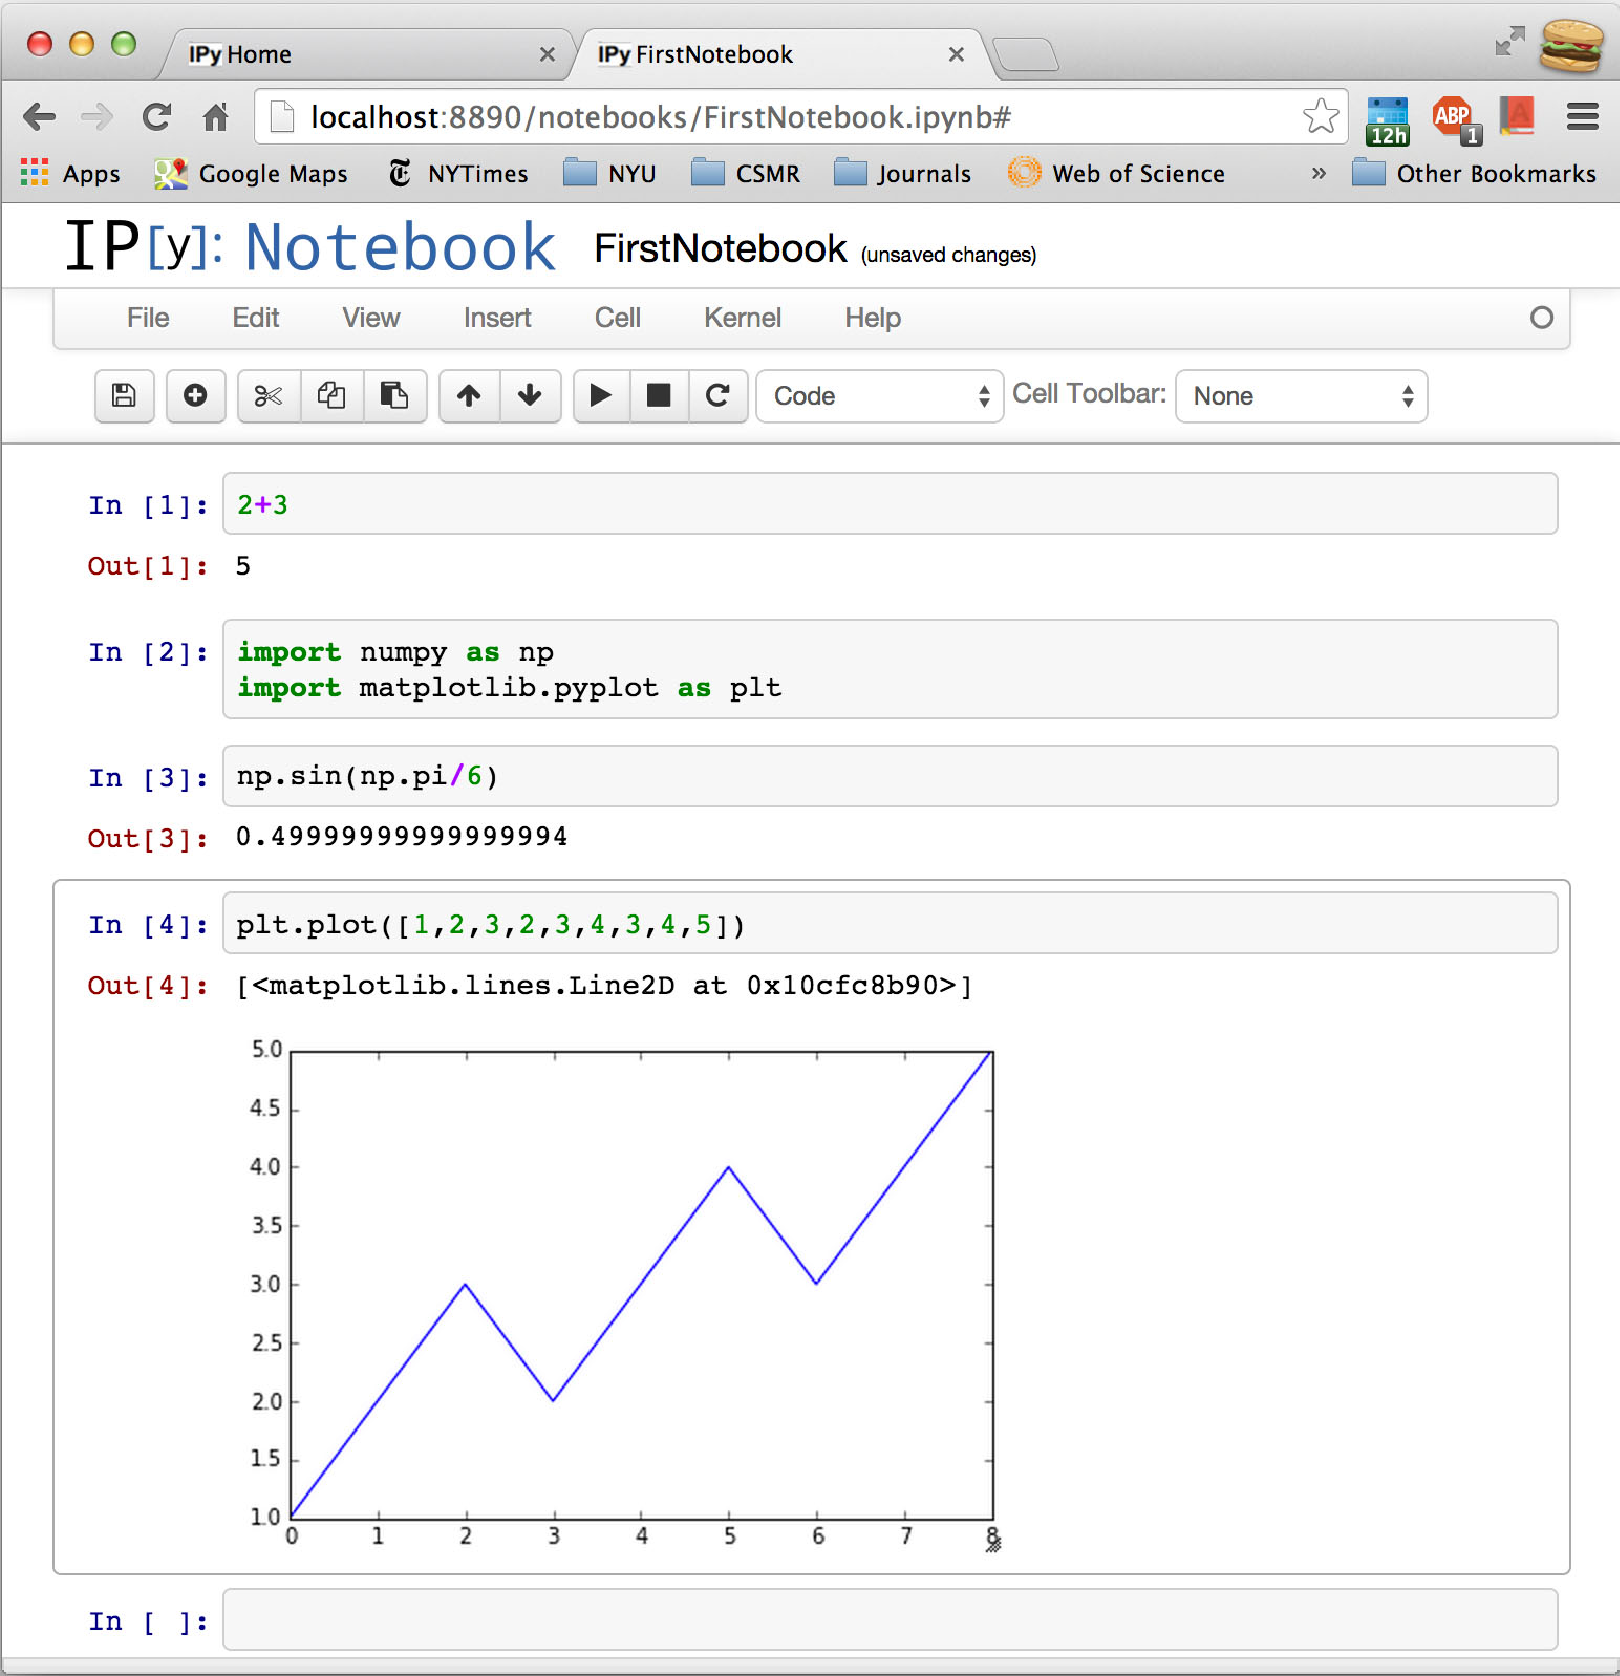
\includegraphics{firstIPyNBcells.pdf}}
\caption{IPython Notebook demo}\label{apdx2/apdx2_ipynb:fig-firstipynbcells}\end{figure}

Below the result a new IPython interactive cell appears ready for your next entry.  In the next cell type the commands to import \code{numpy} and \code{matplotlib.pyplot} as shown in the {\hyperref[apdx2/apdx2_ipynb:fig-firstipynbcells]{\emph{IPython Notebook demo}}} figure.  These two commands are separated by the \code{Shift} (without \code{Enter} or \code{Return}) so that they appear in the same cell.  They are then both executed by pressing \code{Shift-Enter} (or \code{Shift-Return}).

You can also create plots in an IPython notebook.  For example, typing \code{plot({[}1,2,3,2,3,4,3,4,5{]})} and pressing \code{Shift-Enter} produces  the same plot shown in the {\hyperref[chap5/chap5_plot:fig-zigzagplotdemo]{\emph{Interactive plot window}}} figure.  The plot is produced ``in line'' and not in a separate window, because we used the \code{-{-}matplotlib inline} switch when we launched IPython Notebook.  If you have followed along, your IPython notebook should look something like that shown in the figure {\hyperref[apdx2/apdx2_ipynb:fig-firstipynbcells]{\emph{IPython Notebook demo}}}.

Be sure to press the \code{Save and Checkpoint} icon at the far left near the top of the IPython Notebook window from time to time to \textbf{save your work}.


\section{Running programs in an IPython Notebook}
\label{apdx2/apdx2_ipynb:running-programs-in-an-ipython-notebook}
You can also run programs in an IPython notebook.  As an example, we run the program introduced in the section on {\hyperref[chap4/chap4_io:screenoutput]{\emph{Screen output}}}.  The program is input into a single notebook cell and then executed by pressing \code{Shift-Enter}.
\begin{figure}[htbp]
\centering
\capstart

\scalebox{0.800000}{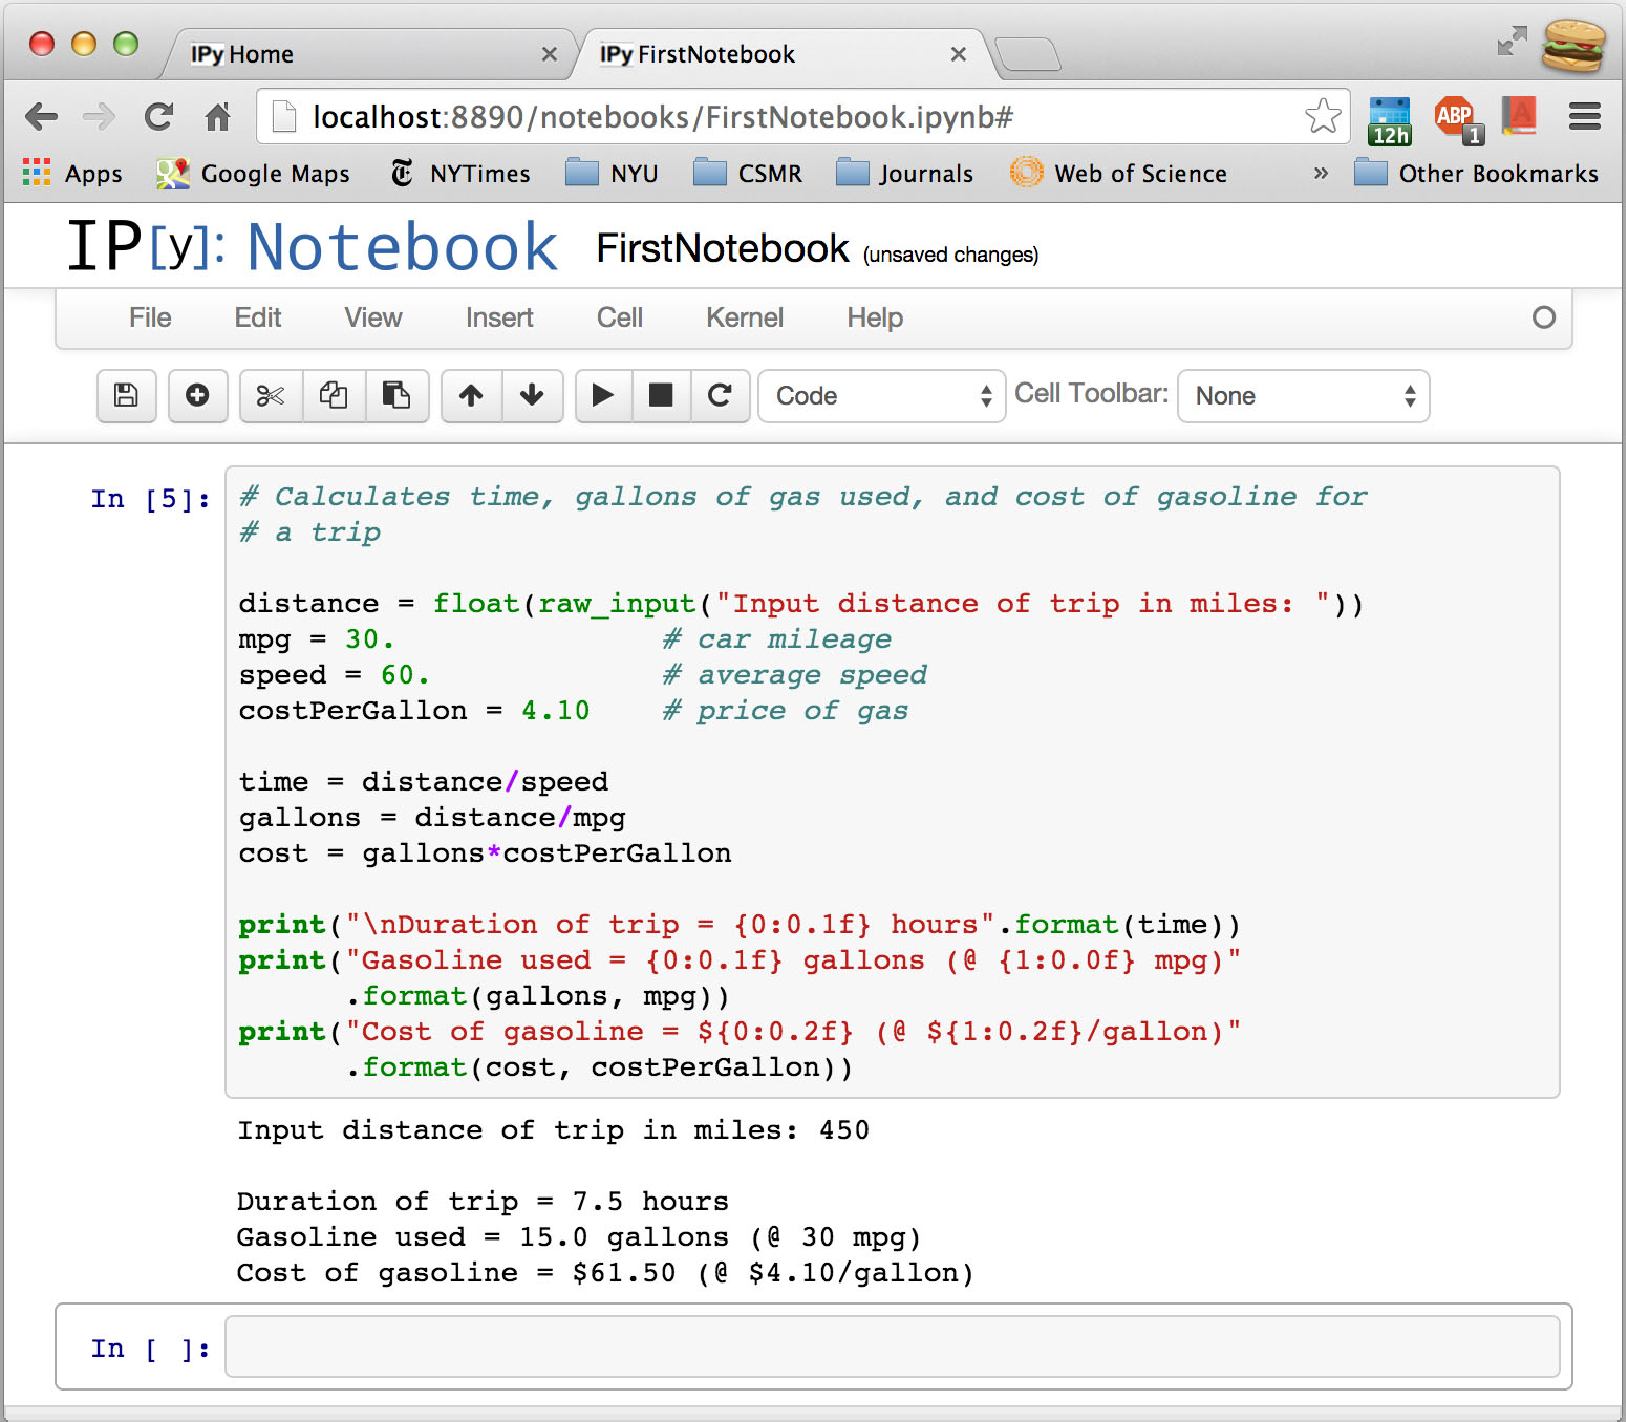
\includegraphics{mileageNB.pdf}}
\caption{Running a program}\label{apdx2/apdx2_ipynb:fig-mileagenb}\end{figure}

In this example, the program requests input from the user: the distance of the trip.  The program runs up to the point where it needs input from the user, and then pauses until the user responds and presses the \code{Enter} or \code{Return} key.  The program then completes its execution.  Thus the IPython notebook provides a complete log of the session.


\section{Annotating an IPython Notebook}
\label{apdx2/apdx2_ipynb:annotating-an-ipython-notebook}
An IPython notebook will be more easily comprehended if it includes annotations of the session.  In addition to logging the inputs and outputs of computations, IPython Notebook allows the user to embed headings, explanatory notes, mathematics, and images.
\begin{figure}[htbp]
\centering
\capstart

\scalebox{0.800000}{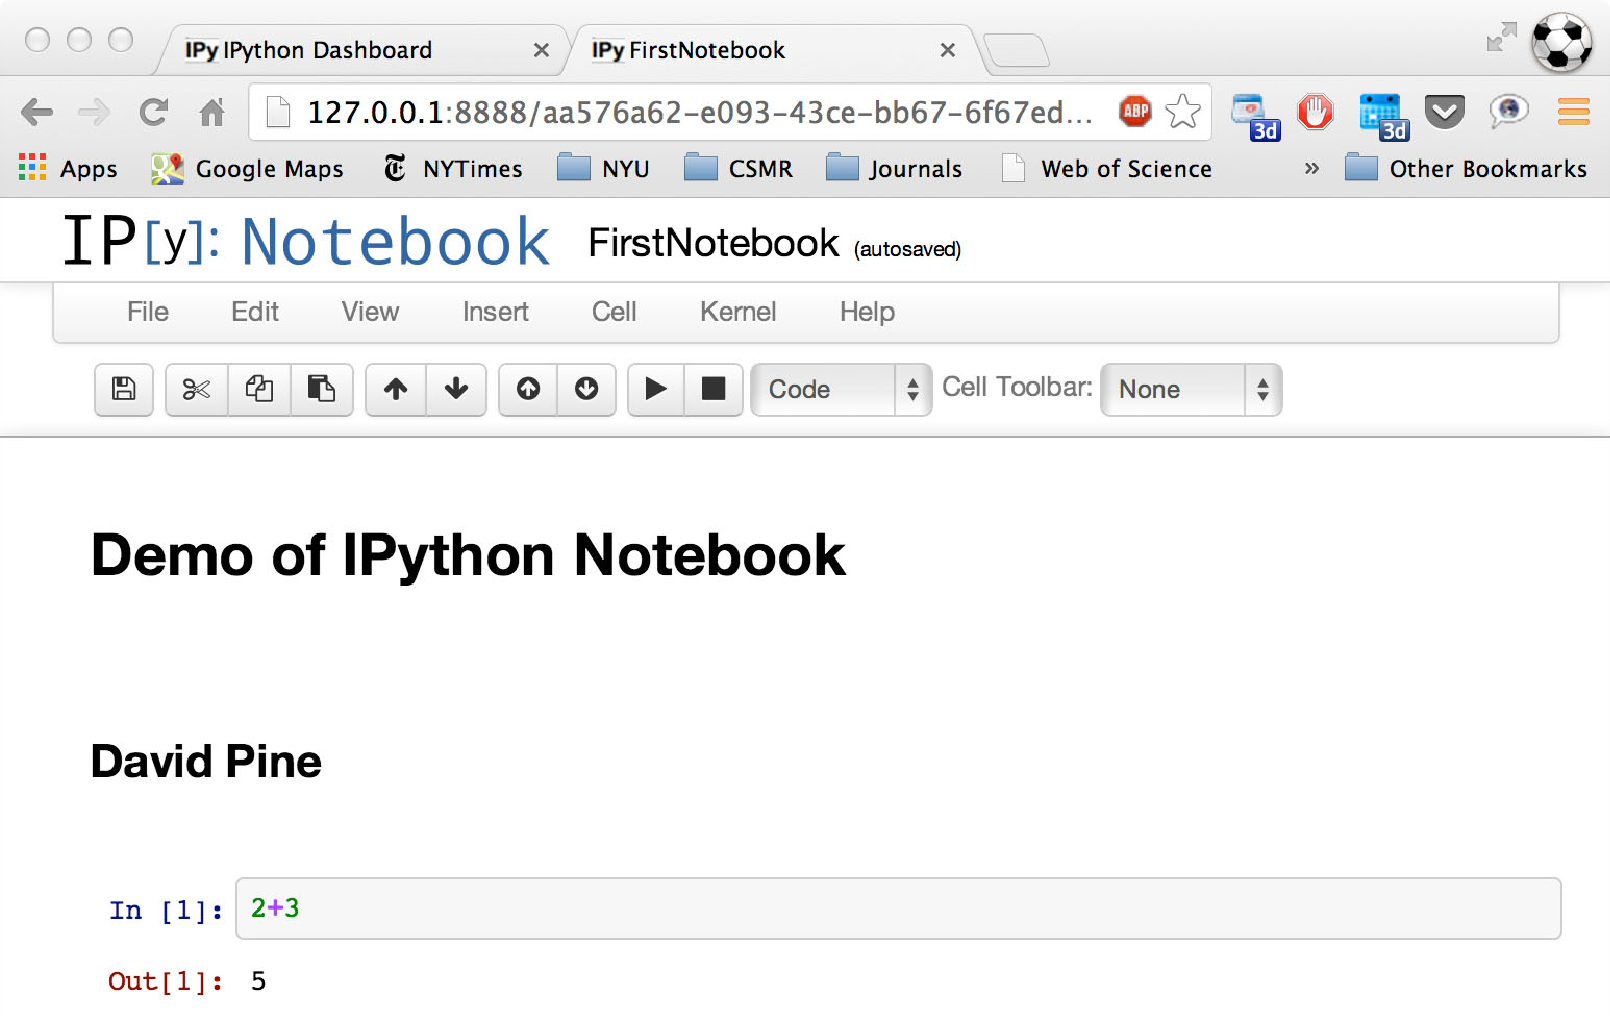
\includegraphics{ipyNoteFinalTop.pdf}}
\caption{Annotating a notebook}\label{apdx2/apdx2_ipynb:fig-ipynotefinaltop}\end{figure}

Suppose, for example, that we want to have a title at the top of the IPython notebook we have been working with, and we want to include the name of the author of the session.  To do this, we scroll the IPython notebook back up to the top and place the cursor and click in the very first input cell, the one that contained \code{2+3}.  We then open the \code{Insert} menu near the top center of the window and click on \code{Insert Cell Above}, which opens up a new input cell above the first cell.  Next, we click on the box in the Toolbar that says \code{Code}.  A list of cell types appears: \code{Code} (currently checked), \code{Markdown}, \code{Raw Text}, \code{Heading 1}, \code{Heading 2}, ..., \code{Heading 6}.  Select \code{Heading 1}; immediately the \code{In {[} {]}:} prompt disappears, indicating that this box is no longer meant for inputing and executing Python code.  Type ``\code{Demo of IPython Notebook}'' and press \code{Shift-Enter} (or \code{Shift-Return}).  A heading in large print appears before the first IPython code cell.  Place the cursor back in the first Ipython code cell (\code{2+3}).  Once again, select the \code{Insert} menu and click on \code{Insert Cell Above}.  Again, click on the Toolbar that says \code{Code}, but this time select \code{Heading 2}.  Type your name into the newly created cell and press \code{Shift-Enter}.  Your name is printed in the cell in slightly smaller print than for the previous case.

You can also write comments, including mathematical expressions, into an IPython Notebook cell.  Let's include a comment after the program we ran that calculated the cost of gasoline for a road trip.  First we place the cursor in the open formula cell below program we ran and then click on the box in the Toolbar that says \code{Code} and change it to \code{Markdown}.  Returning to the cell, we enter the text of our comment.  We can enter any text we wish, including mathematical expressions using the markup language Latex.  (If you do not already know Latex, you can get a brief introduction at these sites: \href{http://en.wikibooks.org/wiki/LaTeX/Mathematics}{http://en.wikibooks.org/wiki/LaTeX/Mathematics} or \href{ftp://ftp.ams.org/pub/tex/doc/amsmath/short-math-guide.pdf}{ftp://ftp.ams.org/pub/tex/doc/amsmath/short-math-guide.pdf}.)  Here we enter the following text:
\begin{quote}

\begin{Verbatim}[commandchars=\\\{\},numbers=left,firstnumber=1,stepnumber=1]
The total distance \PYGZdl{}x\PYGZdl{} traveled during a trip can be
obtained by integrating the velocity \PYGZdl{}v(t)\PYGZdl{} over the
duration \PYGZdl{}T\PYGZdl{} of the trip:
\PYGZbs{}begin\PYGZob{}align\PYGZcb{}
    x = \PYGZbs{}int\PYGZus{}0\PYGZca{}T v(t)\PYGZbs{}, dt
\PYGZbs{}end\PYGZob{}align\PYGZcb{}
\end{Verbatim}
\end{quote}

After entering the text, pressing \code{Shift-Enter} yields the result shown in {\hyperref[apdx2/apdx2_ipynb:fig-markdown]{\emph{Annotation using a Markdown cell}}}.
\begin{figure}[htbp]
\centering
\capstart

\scalebox{0.800000}{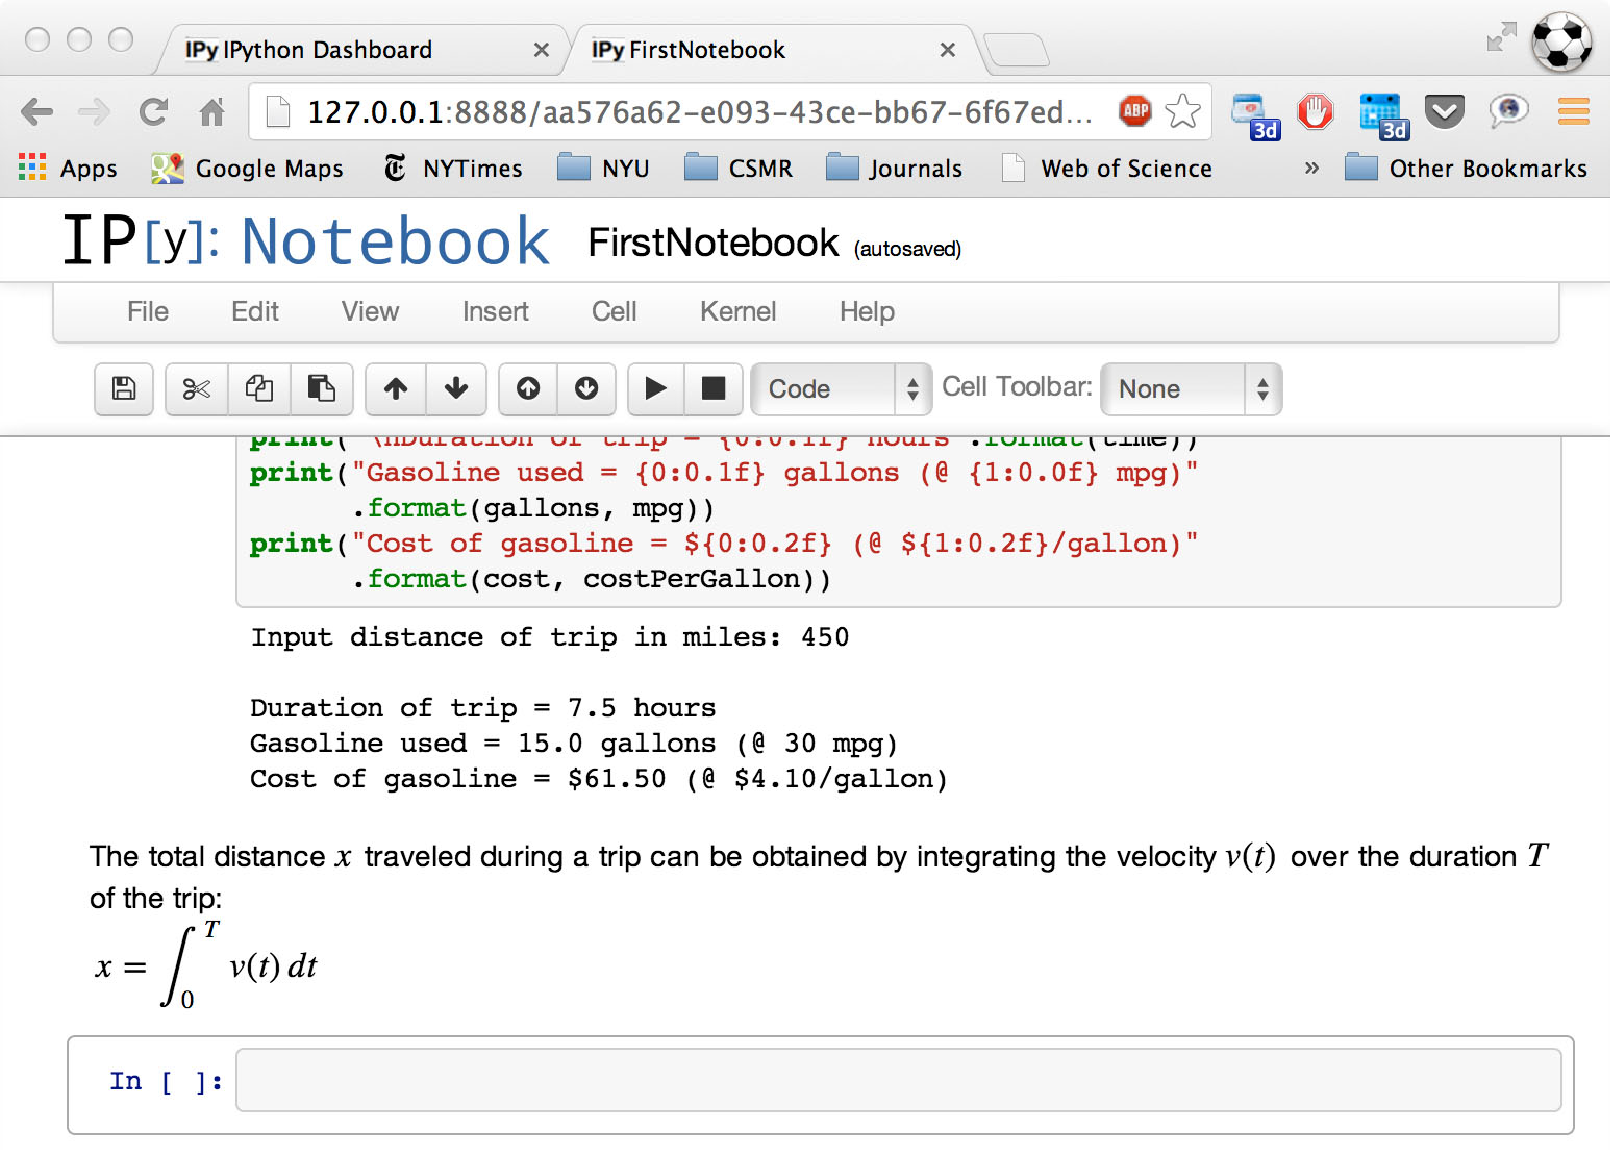
\includegraphics{markdown.pdf}}
\caption{Annotation using a Markdown cell}\label{apdx2/apdx2_ipynb:fig-markdown}\end{figure}

The \code{\$} symbol brackets inline mathematical expressions in Latex, while the \code{\textbackslash{}begin\{align\}} and \code{\textbackslash{}end\{align\}} expressions bracket displayed expressions.  You only need to use Latex if you want to have fancy mathematical expressions in your notes.  Otherwise, they are not necessary.

Suppose you were importing a data (\code{.txt}) file from your hard disk and you wanted to print it out in one of the notebook cells.  If you were in the \code{Terminal} (Mac) or \code{Command Prompt} (PC), you could write the contents of any text file using the command \code{cat} \emph{filename} (Mac) or \code{type} \emph{filename} (PC).  You can execute the same operation from the IPython prompt using the Unix (Mac) or DOS (PC) command preceded by an exclamation point, as described in the section on {\hyperref[chap2/chap2_basics:syscommands]{\emph{System shell commands}}}.
\begin{figure}[htbp]
\centering
\capstart

\scalebox{0.800000}{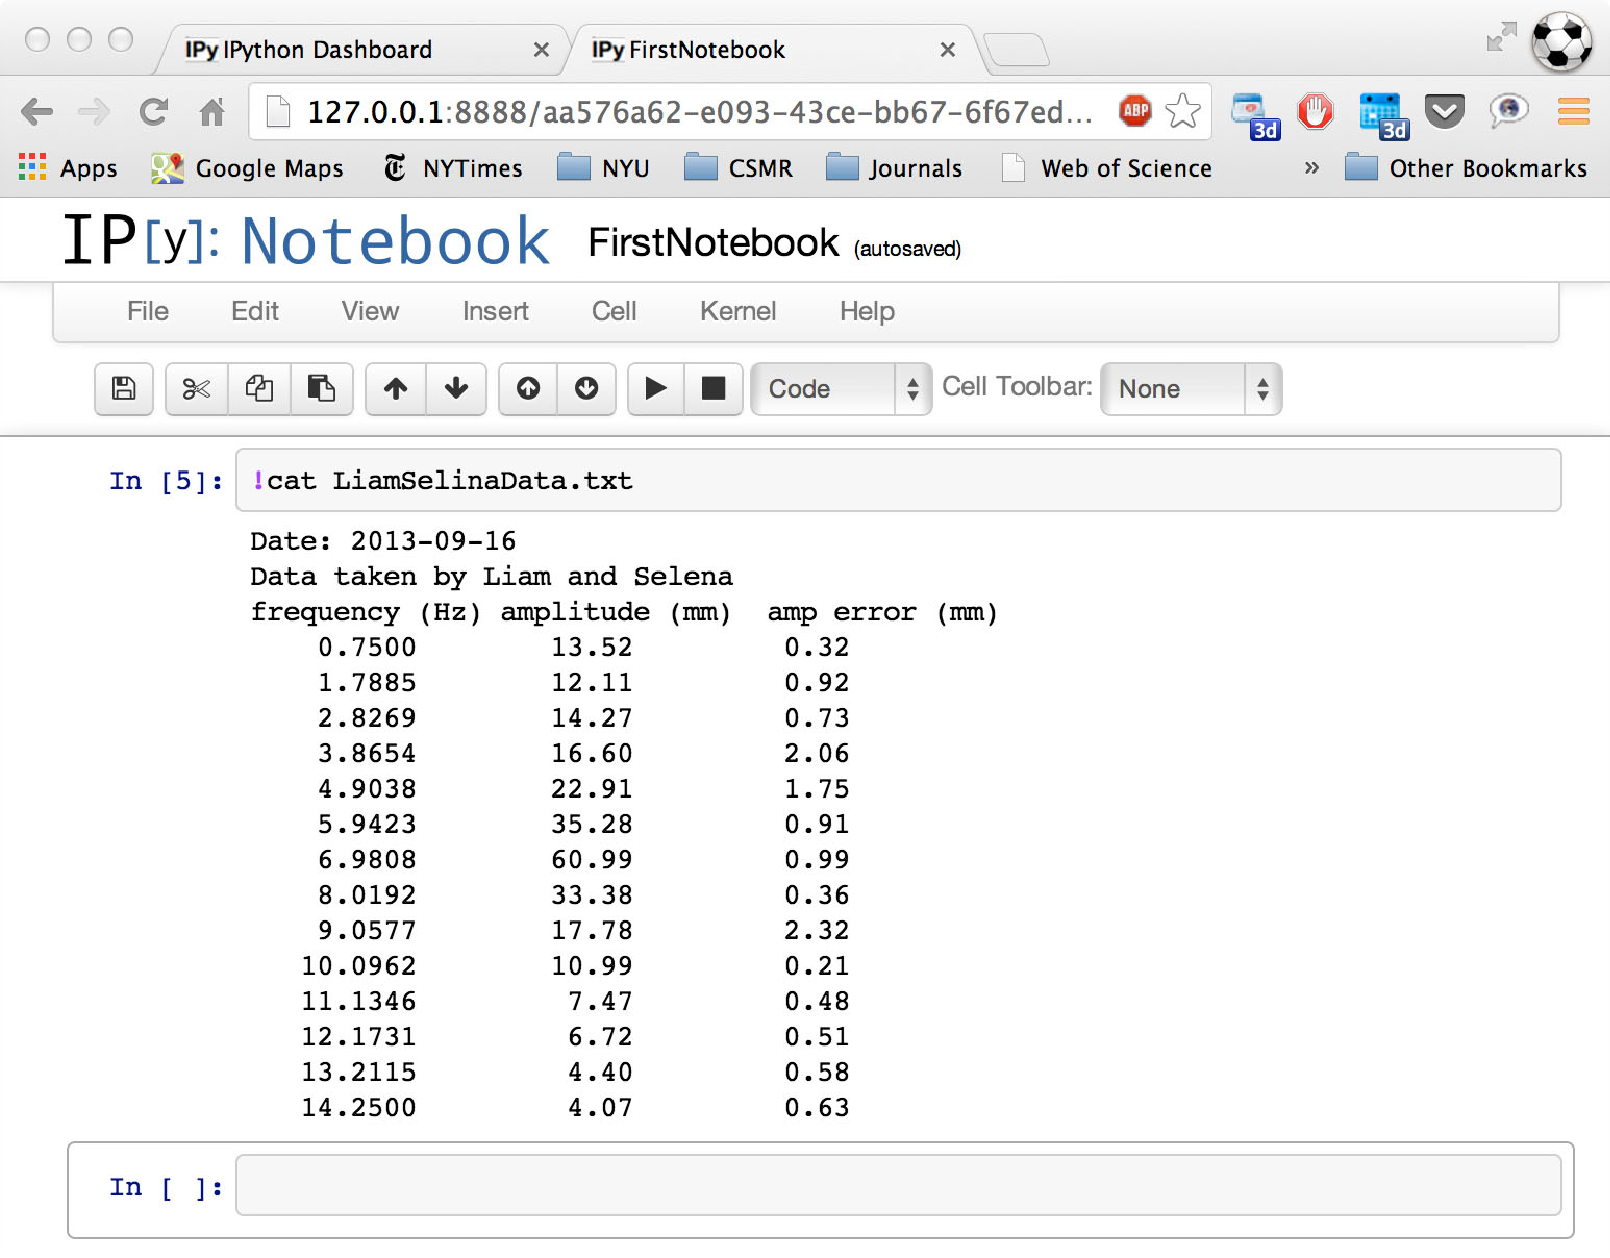
\includegraphics{ipyNoteFinalBottom.pdf}}
\caption{Displaying a text file from disk}\label{apdx2/apdx2_ipynb:fig-ipynotefinalbottom}\end{figure}


\section{Editing and rerunning a notebook}
\label{apdx2/apdx2_ipynb:editing-and-rerunning-a-notebook}
In working with an IPython notebook, you may find that you want to move some cells around, or delete some cells, or simply change some cells.  All of these tasks are possible.  You can  cut and paste cells, as in a normal document editor, using the \code{Edit} menu.  You can also freely edit cells and re-execute them by  pressing \code{Shift-Enter}.  Sometimes you may find that you would like to re-execute the entire notebook afresh.  You can do this by going to the \code{Kernel} menu and selecting \code{Restart}.  A warning message will appear asking you if you really want to restart.  Answer in the affirmative.  Then open the \code{Cell} menu and select \code{Run All}, which will re-execute the notebook starting with the first cell.  You will have to re-enter any screen input requested by the notebook scripts.


\section{Quitting an IPython notebook}
\label{apdx2/apdx2_ipynb:quitting-an-ipython-notebook}
It goes almost without saying that before quitting an IPython notebook, you should make sure you have saved the notebook by pressing the \code{Save and Checkpoint} item in the \code{File} menu or its icon in the Toolbar.

When you are ready to quit working with a notebook, click on the \code{Close and halt} item in the \code{File} menu.  Your notebook browser tab will close and you will return to the IPython Notebook Dashboard.  Just close the IPython Notebook Dashboard tab in your browser to end the session.

Finally, return to the \code{Terminal} or \code{Command Prompt} application, hold down the \code{control} key and press \code{c} twice in rapid succession.  This stops the IPython Notebook session.  You should see the normal system prompt.  You can then close the \code{Terminal} (Mac) or \code{Command Prompt} (PC) session if you wish.


\section{Working with an existing IPython notebook}
\label{apdx2/apdx2_ipynb:working-with-an-existing-ipython-notebook}
To work with an existing IPython notebook, open the \code{Terminal} (Mac) or \code{Command Prompt} (PC) application and navigate to the directory in which the notebook you want to work with resides.  Recall that IPython notebooks have the \code{.ipynb} extension.  Launch the IPython Notebook Dashboard as you did previously by issuing the command
\begin{quote}

\begin{Verbatim}[commandchars=\\\{\}]
ipython notebook \PYGZhy{}\PYGZhy{}matplotlib inline \PYGZam{}
\end{Verbatim}
\end{quote}

This will open the IPython Notebook Dashboard in your web browser, where you should see a list of all the IPython notebooks in that directory (folder).  Click on the name of the notebook you want to open.  It will appear in a new tab on your web browser as before.

Note that while all the input and output from the previous saved session is present, none of it has been run.  That means that none of the variables or other objects has been defined in this new session.  To initialize all the objects in the file, you must rerun the file.  To rerun the file, press the \code{Cell} menu and select \code{Run All}, which will re-execute all the cells.  You will have to re-enter any screen input requested by the notebook scripts.  Now you are ready to pick up where you left off the last time.
\phantomsection\label{apdx3/apdx3_resources::doc}

\chapter{Python Resources}
\label{apdx3/apdx3_resources:apdx3}\label{apdx3/apdx3_resources:python-resources}
This text provides an introduction to Python for science and engineering applications but is hardly exhaustive.  There are many other resources that you will want to tap.  Here I point out several that you may find useful.


\section{Web resources}
\label{apdx3/apdx3_resources:web-resources}
The best web resource for Python is a good search engine like Google.  Nevertheless, I list a few web sites here that you might find useful.  I have successfully resisted any attempt to be exhaustive so that the list is actually useful.  Nevertheless, if you find a really cool site that you think should be on this list, please let me know.
\begin{quote}
\begin{description}
\item[{\href{http://www.python.org/}{http://www.python.org/}}] \leavevmode
The official Python web site.  I almost never look here.

\item[{\href{http://docs.python.org/2/reference/}{http://docs.python.org/2/reference/}}] \leavevmode
Sometimes I look here for detailed information about Python 2, which is the version used in this manual.  Someday, when all the most useful packages are available for Python 3, we will switch to Python 3 and use \href{http://docs.python.org/3/reference/}{http://docs.python.org/3/reference/} instead.

\item[{\href{http://docs.scipy.org/doc/numpy/reference/}{http://docs.scipy.org/doc/numpy/reference/}}] \leavevmode
I usually start here when I need information about NumPy.  It has links to just about all the NumPy documentation I need.  By the way, I say ``num-pee'', which rhymes with ``bumpy''---a lot of people say ``num-pie'', which doesn't sound like English to me.

\item[{\href{http://docs.scipy.org/doc/scipy/reference/}{http://docs.scipy.org/doc/scipy/reference/}}] \leavevmode
I start here when I need information about SciPy, its various packages and their functions.  I say ``psy-pi'' for SciPy, like everyone else.  Who says I have to be consistent? (see Emerson)

\item[{\href{http://matplotlib.org/api/pyplot\_summary.html}{http://matplotlib.org/api/pyplot\_summary.html}}] \leavevmode
The \emph{Plotting Commands Summary} page for MatPlotLib.  It has a search feature and links to all the MatPlotLib documentation, which I use a lot.  You can go the the main MatPlotLib page, \href{http://matplotlib.org/}{http://matplotlib.org/}, but frankly, it's less useful.  The site \href{http://www.loria.fr/~rougier/teaching/matplotlib/}{http://www.loria.fr/\textasciitilde{}rougier/teaching/matplotlib/} is also useful for learning some MatPlotLib tricks.

\item[{\href{http://ipython.org/}{http://ipython.org/}}] \leavevmode
I go to this page mostly to learn about IPython Notebook (\href{http://ipython.org/notebook.html}{http://ipython.org/notebook.html}) but it's also useful if you need information about the IPython interpreter, especially if you want to find out more about IPython magic commands.

\end{description}

\index{Canopy!resources}\begin{description}
\item[{\href{http://www.enthought.com/}{http://www.enthought.com/}}] \leavevmode
I get my latest version of Python and all the packages I need for scientific computing here.  One stop shopping and everything is free for academic users.  They offer three distributions: Express, Basic, and Professional.  Express is free to all users and contains all the Python libraries, NumPy, MatPlotlib, SciPy, \emph{etc}, that are described in this manual.  Basic includes all the packages Enthought supports, which is likely to be everything you will ever need.  Professional adds support services.  Basic is free to academic users.  One nice feature of Canopy is its package manager, which makes it child's play to update or add Python packages.  This is a very nice feature, especially for beginners.  Canopy displaces the older Enthought EPD packages.

\end{description}

\index{Spyder!resources}\begin{description}
\item[{\href{https://code.google.com/p/spyderlib/}{https://code.google.com/p/spyderlib/}}] \leavevmode
Get the latest version of Spyder, the alternative IDE to Enthought's Canopy.  Sypder is completely open source and has a number of nice features, like introspection, not currently available in Canopy.  Spyder is very popular and can be installed easily on all platforms.  For an effective package manager, see Anaconda (next entry).

\end{description}

\index{Anaconda!resources}\begin{description}
\item[{\href{http://continuum.io/}{http://continuum.io/}}] \leavevmode
Anaconda provides a free distribution of Spyder with a comprehensive package manager, and may be the best choice for power users of Python for scientific programming.  The package manager is run by line commands from a terminal window, which may put off beginners.  Anaconda can be downloaded from \href{https://store.continuum.io/cshop/anaconda/}{https://store.continuum.io/cshop/anaconda/}.

\item[{\href{http://www.scipy.org/Mailing\_Lists}{http://www.scipy.org/Mailing\_Lists}}] \leavevmode
Go here if you want to sign up for a mailing list for NumPy or SciPy, or if you want to report a bug.  Mailing lists give you access to a community of developers and users that can often provide expert help.  Just remember to be polite and respectful of those helping you and also to those posting questions.

\item[{\href{https://lists.sourceforge.net/lists/listinfo/matplotlib-users}{https://lists.sourceforge.net/lists/listinfo/matplotlib-users}}] \leavevmode
The mailing list for MatPlotLib.  See paragraph immediately above.

\item[{\href{http://stackoverflow.com/}{http://stackoverflow.com/}}] \leavevmode
StackOverflow may just be your best friend when it comes to solving problems using Python.  You pose your question about whatever problem you are having with Python and other people write answers.  The answers are monitored and the best survive.  In fact, most of the questions you will pose have already been posed by someone else and answered.  So you can just look up the answer to most of your questions.  StackOverflow is a wonderful resource.

\end{description}
\end{quote}


\section{Books}
\label{apdx3/apdx3_resources:books}
There are a lot of books on Python and there is no way I can provide reviews for all of them.  I have found that the book by Mark Lutz, \emph{Learning Python}, published by O'Reilly Media does the trick for most people.  It doesn't have anything special for scientific programming, and thus does not cover the NumPy, SciPy, or MatPlotLib packages, but for just about everything else, it's an excellent resource.  It gives a good introduction to object oriented programming, or OOP, which I say little about in this text.  The 3rd edition of the book covers Python 2 while the 4th and 5th (current) editions cover Python 3.  You are probably better off getting the latest edition as everybody will soon be using Python 3.  If you are using Python 2, as we do in this text, you can easily enough figure out the differences between Python 3 and 2.



\renewcommand{\indexname}{Index}
\printindex
\end{document}
